\documentclass[a4paper]{book}
\usepackage{a4wide}
\usepackage{makeidx}
\usepackage{fancyhdr}
\usepackage{graphicx}
\usepackage{multicol}
\usepackage{float}
\usepackage{textcomp}
\usepackage{alltt}
\usepackage[utf8]{inputenc}
\usepackage{doxygen}
\makeindex
\setcounter{tocdepth}{3}
\renewcommand{\footrulewidth}{0.4pt}
\begin{document}
\begin{titlepage}
\vspace*{7cm}
\begin{center}
{\Large hive \\[1ex]\large 0.00 }\\
\vspace*{1cm}
{\large Generated by Doxygen 1.5.6}\\
\vspace*{0.5cm}
{\small Mon Oct 19 17:23:29 2009}\\
\end{center}
\end{titlepage}
\clearemptydoublepage
\pagenumbering{roman}
\tableofcontents
\clearemptydoublepage
\pagenumbering{arabic}
\chapter{Todo List}
\label{todo}
\label{todo__todo000001}
 \begin{description}
\item[Class \doxyref{Hive::Action}{p.}{classHive_1_1Action} ]everything

\end{description}


\label{todo__todo000002}
 \begin{description}
\item[Class \doxyref{Hive::Agent}{p.}{classHive_1_1Agent} ]Everything

\end{description}


\label{todo__todo000003}
 \begin{description}
\item[Class \doxyref{Hive::AgentFactory}{p.}{classHive_1_1AgentFactory} ]Everything

\end{description}


\label{todo__todo000010}
 \begin{description}
\item[Class \doxyref{Hive::Composer}{p.}{classHive_1_1Composer} ]Everything

\end{description}


\label{todo__todo000004}
 \begin{description}
\item[Class \doxyref{Hive::Data}{p.}{classHive_1_1Data} ]

\end{description}


\label{todo__todo000005}
 \begin{description}
\item[Class \doxyref{Hive::Database}{p.}{classHive_1_1Database} ]Implementation

\end{description}


\label{todo__todo000017}
 \begin{description}
\item[Class \doxyref{Dummy::DummyMessageGenerator}{p.}{classDummy_1_1DummyMessageGenerator} ]

\end{description}


\label{todo__todo000018}
 \begin{description}
\item[Class \doxyref{Dummy::DummyWaveAction}{p.}{classDummy_1_1DummyWaveAction} ]error-checking whether the counter exists in the agent

\end{description}


\label{todo__todo000013}
 \begin{description}
\item[Class \doxyref{Hive::InputDataReader}{p.}{classHive_1_1InputDataReader} ]Everything

\end{description}


\label{todo__todo000015}
 \begin{description}
\item[Class \doxyref{Hive::InputSystemReader}{p.}{classHive_1_1InputSystemReader} ]everything

\end{description}


\label{todo__todo000006}
 \begin{description}
\item[Class \doxyref{Hive::Message}{p.}{classHive_1_1Message} ]everything. how do we specify the parameters ?!

\end{description}


\label{todo__todo000009}
 \begin{description}
\item[Class \doxyref{Hive::SerialCommunicator}{p.}{classHive_1_1SerialCommunicator} ]

\end{description}


\label{todo__todo000019}
 \begin{description}
\item[Class \doxyref{Hive::Simulator}{p.}{classHive_1_1Simulator} ]everything

\end{description}


\label{todo__todo000014}
 \begin{description}
\item[Class \doxyref{Hive::System}{p.}{classHive_1_1System} ]everything, more conceptional work needed. will we have prototypes of agents in here?! it should be a database of types ... whatever ...

\end{description}


\label{todo__todo000011}
 \begin{description}
\item[File \doxyref{hive.cpp}{p.}{hive_8cpp} ]Fill in the details.

\end{description}


\label{todo__todo000012}
 \begin{description}
\item[File \doxyref{hive.hh}{p.}{hive_8hh} ]Fill in the details.

\end{description}

\chapter{Bug List}
\label{bug}
\label{bug__bug000001}
 \begin{description}
\item[Class \doxyref{Hive::Action}{p.}{classHive_1_1Action} ]

\end{description}


\label{bug__bug000002}
 \begin{description}
\item[Class \doxyref{Hive::Agent}{p.}{classHive_1_1Agent} ]

\end{description}


\label{bug__bug000003}
 \begin{description}
\item[Class \doxyref{Hive::AgentFactory}{p.}{classHive_1_1AgentFactory} ]who know's?

\end{description}


\label{bug__bug000006}
 \begin{description}
\item[Class \doxyref{Hive::InputDataReader}{p.}{classHive_1_1InputDataReader} ]unknown as of yet

\end{description}


\label{bug__bug000008}
 \begin{description}
\item[Class \doxyref{Hive::InputSystemReader}{p.}{classHive_1_1InputSystemReader} ]

\end{description}


\label{bug__bug000004}
 \begin{description}
\item[Class \doxyref{Hive::Message}{p.}{classHive_1_1Message} ]

\end{description}


\label{bug__bug000010}
 \begin{description}
\item[Class \doxyref{Hive::Simulator}{p.}{classHive_1_1Simulator} ]

\end{description}


\label{bug__bug000007}
 \begin{description}
\item[Class \doxyref{Hive::System}{p.}{classHive_1_1System} ]

\end{description}

\chapter{Deprecated List}
\label{deprecated}
\label{deprecated__deprecated000001}
 \begin{description}
\item[Member \doxyref{TiXmlHandle::Node}{p.}{classTiXmlHandle_b44b723a8dc9af72838a303c079d0376}() const  ]use ToNode. Return the handle as a \doxyref{TiXmlNode}{p.}{classTiXmlNode}. This may return null. \end{description}


\label{deprecated__deprecated000002}
 \begin{description}
\item[Member \doxyref{TiXmlHandle::Element}{p.}{classTiXmlHandle_cb5fe8388a526289ea65e817a51e05e7}() const  ]use ToElement. Return the handle as a \doxyref{TiXmlElement}{p.}{classTiXmlElement}. This may return null. \end{description}


\label{deprecated__deprecated000003}
 \begin{description}
\item[Member \doxyref{TiXmlHandle::Text}{p.}{classTiXmlHandle_9fc739c8a18d160006f82572fc143d13}() const  ]use ToText() Return the handle as a \doxyref{TiXmlText}{p.}{classTiXmlText}. This may return null. \end{description}


\label{deprecated__deprecated000004}
 \begin{description}
\item[Member \doxyref{TiXmlHandle::Unknown}{p.}{classTiXmlHandle_49675b74357ba2aae124657a9a1ef465}() const  ]use ToUnknown() Return the handle as a \doxyref{TiXmlUnknown}{p.}{classTiXmlUnknown}. This may return null. \end{description}

\chapter{Namespace Index}
\section{Namespace List}
Here is a list of all namespaces with brief descriptions:\begin{CompactList}
\item\contentsline{section}{{\bf Dummy} }{\pageref{namespaceDummy}}{}
\item\contentsline{section}{{\bf Hive} (Core \doxyref{Hive}{p.}{namespaceHive} classes and functionality )}{\pageref{namespaceHive}}{}
\item\contentsline{section}{{\bf mu} (Namespace for mathematical applications )}{\pageref{namespacemu}}{}
\item\contentsline{section}{{\bf Util} (General utility function library )}{\pageref{namespaceUtil}}{}
\end{CompactList}

\chapter{Class Index}
\section{Class Hierarchy}
This inheritance list is sorted roughly, but not completely, alphabetically:\begin{CompactList}
\item \contentsline{section}{Hive::Action}{\pageref{classHive_1_1Action}}{}
\begin{CompactList}
\item \contentsline{section}{Dummy::DummyWaveAction}{\pageref{classDummy_1_1DummyWaveAction}}{}
\end{CompactList}
\item \contentsline{section}{Hive::Agent}{\pageref{classHive_1_1Agent}}{}
\item \contentsline{section}{Hive::AgentFactory}{\pageref{classHive_1_1AgentFactory}}{}
\begin{CompactList}
\item \contentsline{section}{Dummy::DummyAgentFactory}{\pageref{classDummy_1_1DummyAgentFactory}}{}
\end{CompactList}
\item \contentsline{section}{Hive::Communicator}{\pageref{classHive_1_1Communicator}}{}
\begin{CompactList}
\item \contentsline{section}{Hive::SerialCommunicator}{\pageref{classHive_1_1SerialCommunicator}}{}
\end{CompactList}
\item \contentsline{section}{Hive::Composer}{\pageref{classHive_1_1Composer}}{}
\begin{CompactList}
\item \contentsline{section}{Dummy::DummyComposer}{\pageref{classDummy_1_1DummyComposer}}{}
\end{CompactList}
\item \contentsline{section}{Hive::Data}{\pageref{classHive_1_1Data}}{}
\begin{CompactList}
\item \contentsline{section}{Hive::BoolData}{\pageref{classHive_1_1BoolData}}{}
\item \contentsline{section}{Hive::DoubleData}{\pageref{classHive_1_1DoubleData}}{}
\item \contentsline{section}{Hive::IntegerData}{\pageref{classHive_1_1IntegerData}}{}
\end{CompactList}
\item \contentsline{section}{Hive::Database}{\pageref{classHive_1_1Database}}{}
\item \contentsline{section}{Hive::InputDataReader}{\pageref{classHive_1_1InputDataReader}}{}
\item \contentsline{section}{Hive::InputSystemReader}{\pageref{classHive_1_1InputSystemReader}}{}
\item \contentsline{section}{Hive::Message}{\pageref{classHive_1_1Message}}{}
\item \contentsline{section}{Hive::MessageGenerator}{\pageref{classHive_1_1MessageGenerator}}{}
\begin{CompactList}
\item \contentsline{section}{Dummy::DummyMessageGenerator}{\pageref{classDummy_1_1DummyMessageGenerator}}{}
\end{CompactList}
\item \contentsline{section}{MTRand\_\-int32}{\pageref{classMTRand__int32}}{}
\begin{CompactList}
\item \contentsline{section}{MTRand}{\pageref{classMTRand}}{}
\item \contentsline{section}{MTRand53}{\pageref{classMTRand53}}{}
\item \contentsline{section}{MTRand\_\-closed}{\pageref{classMTRand__closed}}{}
\item \contentsline{section}{MTRand\_\-open}{\pageref{classMTRand__open}}{}
\end{CompactList}
\item \contentsline{section}{Hive::OutputWriter}{\pageref{classHive_1_1OutputWriter}}{}
\item \contentsline{section}{mu::ParserBase}{\pageref{classmu_1_1ParserBase}}{}
\begin{CompactList}
\item \contentsline{section}{mu::Parser}{\pageref{classmu_1_1Parser}}{}
\item \contentsline{section}{mu::ParserComplex}{\pageref{classmu_1_1ParserComplex}}{}
\item \contentsline{section}{mu::ParserInt}{\pageref{classmu_1_1ParserInt}}{}
\end{CompactList}
\item \contentsline{section}{mu::ParserByteCode}{\pageref{classmu_1_1ParserByteCode}}{}
\item \contentsline{section}{mu::ParserCallback}{\pageref{classmu_1_1ParserCallback}}{}
\item \contentsline{section}{mu::ParserError}{\pageref{classmu_1_1ParserError}}{}
\item \contentsline{section}{mu::ParserErrorMsg}{\pageref{classmu_1_1ParserErrorMsg}}{}
\item \contentsline{section}{mu::ParserStack$<$ TValueType $>$}{\pageref{classmu_1_1ParserStack}}{}
\item \contentsline{section}{mu::ParserToken$<$ TBase, TString $>$}{\pageref{classmu_1_1ParserToken}}{}
\item \contentsline{section}{mu::ParserTokenReader}{\pageref{classmu_1_1ParserTokenReader}}{}
\item \contentsline{section}{Hive::Simulator}{\pageref{classHive_1_1Simulator}}{}
\begin{CompactList}
\item \contentsline{section}{Hive::DummySimulator}{\pageref{classHive_1_1DummySimulator}}{}
\end{CompactList}
\item \contentsline{section}{mu::STATIC\_\-ASSERTION\_\-FAILURE$<$ true $>$}{\pageref{structmu_1_1STATIC__ASSERTION__FAILURE_3_01true_01_4}}{}
\item \contentsline{section}{Hive::System}{\pageref{classHive_1_1System}}{}
\item \contentsline{section}{TiXmlAttributeSet}{\pageref{classTiXmlAttributeSet}}{}
\item \contentsline{section}{TiXmlBase}{\pageref{classTiXmlBase}}{}
\begin{CompactList}
\item \contentsline{section}{TiXmlAttribute}{\pageref{classTiXmlAttribute}}{}
\item \contentsline{section}{TiXmlNode}{\pageref{classTiXmlNode}}{}
\begin{CompactList}
\item \contentsline{section}{TiXmlComment}{\pageref{classTiXmlComment}}{}
\item \contentsline{section}{TiXmlDeclaration}{\pageref{classTiXmlDeclaration}}{}
\item \contentsline{section}{TiXmlDocument}{\pageref{classTiXmlDocument}}{}
\item \contentsline{section}{TiXmlElement}{\pageref{classTiXmlElement}}{}
\item \contentsline{section}{TiXmlText}{\pageref{classTiXmlText}}{}
\item \contentsline{section}{TiXmlUnknown}{\pageref{classTiXmlUnknown}}{}
\end{CompactList}
\end{CompactList}
\item \contentsline{section}{TiXmlCursor}{\pageref{structTiXmlCursor}}{}
\item \contentsline{section}{TiXmlHandle}{\pageref{classTiXmlHandle}}{}
\item \contentsline{section}{TiXmlParsingData}{\pageref{classTiXmlParsingData}}{}
\item \contentsline{section}{TiXmlString}{\pageref{classTiXmlString}}{}
\begin{CompactList}
\item \contentsline{section}{TiXmlOutStream}{\pageref{classTiXmlOutStream}}{}
\end{CompactList}
\item \contentsline{section}{TiXmlVisitor}{\pageref{classTiXmlVisitor}}{}
\begin{CompactList}
\item \contentsline{section}{TiXmlPrinter}{\pageref{classTiXmlPrinter}}{}
\end{CompactList}
\end{CompactList}

\chapter{Class Index}
\section{Class List}
Here are the classes, structs, unions and interfaces with brief descriptions:\begin{CompactList}
\item\contentsline{section}{{\bf Hive::Action} (\doxyref{Action}{p.}{classHive_1_1Action} class for working on an agent )}{\pageref{classHive_1_1Action}}{}
\item\contentsline{section}{{\bf Hive::Agent} (Central class of the hive )}{\pageref{classHive_1_1Agent}}{}
\item\contentsline{section}{{\bf Hive::AgentFactory} (\doxyref{Agent}{p.}{classHive_1_1Agent} factory )}{\pageref{classHive_1_1AgentFactory}}{}
\item\contentsline{section}{{\bf Hive::BoolData} (A data object to store integer values )}{\pageref{classHive_1_1BoolData}}{}
\item\contentsline{section}{{\bf Hive::Communicator} }{\pageref{classHive_1_1Communicator}}{}
\item\contentsline{section}{{\bf Hive::Composer} (This class sets up the entire simulation )}{\pageref{classHive_1_1Composer}}{}
\item\contentsline{section}{{\bf Hive::Data} (Individual element of the database )}{\pageref{classHive_1_1Data}}{}
\item\contentsline{section}{{\bf Hive::Database} (\doxyref{Database}{p.}{classHive_1_1Database} of an agent )}{\pageref{classHive_1_1Database}}{}
\item\contentsline{section}{{\bf Hive::DoubleData} (A data object to store double values )}{\pageref{classHive_1_1DoubleData}}{}
\item\contentsline{section}{{\bf Dummy::DummyAgentFactory} (Simple implementation of an agentfactory )}{\pageref{classDummy_1_1DummyAgentFactory}}{}
\item\contentsline{section}{{\bf Dummy::DummyComposer} }{\pageref{classDummy_1_1DummyComposer}}{}
\item\contentsline{section}{{\bf Dummy::DummyMessageGenerator} (This class implements the messagegenerator )}{\pageref{classDummy_1_1DummyMessageGenerator}}{}
\item\contentsline{section}{{\bf Hive::DummySimulator} }{\pageref{classHive_1_1DummySimulator}}{}
\item\contentsline{section}{{\bf Dummy::DummyWaveAction} (This is a dummy implementation of the action class )}{\pageref{classDummy_1_1DummyWaveAction}}{}
\item\contentsline{section}{{\bf Hive::InputDataReader} (Reads input from filestream )}{\pageref{classHive_1_1InputDataReader}}{}
\item\contentsline{section}{{\bf Hive::InputSystemReader} (Abstract class for reading a system )}{\pageref{classHive_1_1InputSystemReader}}{}
\item\contentsline{section}{{\bf Hive::IntegerData} (A data object to store integer values )}{\pageref{classHive_1_1IntegerData}}{}
\item\contentsline{section}{{\bf Hive::Message} (\doxyref{Message}{p.}{classHive_1_1Message} for agent communication )}{\pageref{classHive_1_1Message}}{}
\item\contentsline{section}{{\bf Hive::MessageGenerator} }{\pageref{classHive_1_1MessageGenerator}}{}
\item\contentsline{section}{{\bf MTRand} }{\pageref{classMTRand}}{}
\item\contentsline{section}{{\bf MTRand53} }{\pageref{classMTRand53}}{}
\item\contentsline{section}{{\bf MTRand\_\-closed} }{\pageref{classMTRand__closed}}{}
\item\contentsline{section}{{\bf MTRand\_\-int32} }{\pageref{classMTRand__int32}}{}
\item\contentsline{section}{{\bf MTRand\_\-open} }{\pageref{classMTRand__open}}{}
\item\contentsline{section}{{\bf Hive::OutputWriter} }{\pageref{classHive_1_1OutputWriter}}{}
\item\contentsline{section}{{\bf mu::Parser} (Mathematical expressions parser )}{\pageref{classmu_1_1Parser}}{}
\item\contentsline{section}{{\bf mu::ParserBase} (Mathematical expressions parser (base parser engine) )}{\pageref{classmu_1_1ParserBase}}{}
\item\contentsline{section}{{\bf mu::ParserByteCode} (Bytecode implementation of the Math \doxyref{Parser}{p.}{classmu_1_1Parser} )}{\pageref{classmu_1_1ParserByteCode}}{}
\item\contentsline{section}{{\bf mu::ParserCallback} (Encapsulation of prototypes for a numerical parser function )}{\pageref{classmu_1_1ParserCallback}}{}
\item\contentsline{section}{{\bf mu::ParserComplex} (Mathematical expressions parser )}{\pageref{classmu_1_1ParserComplex}}{}
\item\contentsline{section}{{\bf mu::ParserError} (Error class of the parser )}{\pageref{classmu_1_1ParserError}}{}
\item\contentsline{section}{{\bf mu::ParserErrorMsg} (A class that handles the error messages )}{\pageref{classmu_1_1ParserErrorMsg}}{}
\item\contentsline{section}{{\bf mu::ParserInt} (Mathematical expressions parser )}{\pageref{classmu_1_1ParserInt}}{}
\item\contentsline{section}{{\bf mu::ParserStack$<$ TValueType $>$} (\doxyref{Parser}{p.}{classmu_1_1Parser} stack implementation )}{\pageref{classmu_1_1ParserStack}}{}
\item\contentsline{section}{{\bf mu::ParserToken$<$ TBase, TString $>$} (Encapsulation of the data for a single formula token )}{\pageref{classmu_1_1ParserToken}}{}
\item\contentsline{section}{{\bf mu::ParserTokenReader} (Token reader for the \doxyref{ParserBase}{p.}{classmu_1_1ParserBase} class )}{\pageref{classmu_1_1ParserTokenReader}}{}
\item\contentsline{section}{{\bf Hive::SerialCommunicator} (Serialcommunicator implements the communicator )}{\pageref{classHive_1_1SerialCommunicator}}{}
\item\contentsline{section}{{\bf Hive::Simulator} (\doxyref{Simulator}{p.}{classHive_1_1Simulator} class )}{\pageref{classHive_1_1Simulator}}{}
\item\contentsline{section}{{\bf mu::STATIC\_\-ASSERTION\_\-FAILURE$<$ true $>$} }{\pageref{structmu_1_1STATIC__ASSERTION__FAILURE_3_01true_01_4}}{}
\item\contentsline{section}{{\bf Hive::System} (\doxyref{System}{p.}{classHive_1_1System} class )}{\pageref{classHive_1_1System}}{}
\item\contentsline{section}{{\bf TiXmlAttribute} }{\pageref{classTiXmlAttribute}}{}
\item\contentsline{section}{{\bf TiXmlAttributeSet} }{\pageref{classTiXmlAttributeSet}}{}
\item\contentsline{section}{{\bf TiXmlBase} }{\pageref{classTiXmlBase}}{}
\item\contentsline{section}{{\bf TiXmlComment} }{\pageref{classTiXmlComment}}{}
\item\contentsline{section}{{\bf TiXmlCursor} }{\pageref{structTiXmlCursor}}{}
\item\contentsline{section}{{\bf TiXmlDeclaration} }{\pageref{classTiXmlDeclaration}}{}
\item\contentsline{section}{{\bf TiXmlDocument} }{\pageref{classTiXmlDocument}}{}
\item\contentsline{section}{{\bf TiXmlElement} }{\pageref{classTiXmlElement}}{}
\item\contentsline{section}{{\bf TiXmlHandle} }{\pageref{classTiXmlHandle}}{}
\item\contentsline{section}{{\bf TiXmlNode} }{\pageref{classTiXmlNode}}{}
\item\contentsline{section}{{\bf TiXmlOutStream} }{\pageref{classTiXmlOutStream}}{}
\item\contentsline{section}{{\bf TiXmlParsingData} }{\pageref{classTiXmlParsingData}}{}
\item\contentsline{section}{{\bf TiXmlPrinter} }{\pageref{classTiXmlPrinter}}{}
\item\contentsline{section}{{\bf TiXmlString} }{\pageref{classTiXmlString}}{}
\item\contentsline{section}{{\bf TiXmlText} }{\pageref{classTiXmlText}}{}
\item\contentsline{section}{{\bf TiXmlUnknown} }{\pageref{classTiXmlUnknown}}{}
\item\contentsline{section}{{\bf TiXmlVisitor} }{\pageref{classTiXmlVisitor}}{}
\end{CompactList}

\chapter{File Index}
\section{File List}
Here is a list of all files with brief descriptions:\begin{CompactList}
\item\contentsline{section}{{\bf agent.cpp} }{\pageref{agent_8cpp}}{}
\item\contentsline{section}{{\bf agent.hh} }{\pageref{agent_8hh}}{}
\item\contentsline{section}{{\bf agent\_\-factory.hh} }{\pageref{agent__factory_8hh}}{}
\item\contentsline{section}{{\bf arnie.hh} }{\pageref{arnie_8hh}}{}
\item\contentsline{section}{{\bf commandLineParser.cpp} }{\pageref{commandLineParser_8cpp}}{}
\item\contentsline{section}{{\bf commandLineParser.hh} }{\pageref{commandLineParser_8hh}}{}
\item\contentsline{section}{{\bf communicator.hh} }{\pageref{communicator_8hh}}{}
\item\contentsline{section}{{\bf composer.hh} }{\pageref{composer_8hh}}{}
\item\contentsline{section}{{\bf constants.hh} }{\pageref{constants_8hh}}{}
\item\contentsline{section}{{\bf conversion.cpp} }{\pageref{conversion_8cpp}}{}
\item\contentsline{section}{{\bf conversion.hh} }{\pageref{conversion_8hh}}{}
\item\contentsline{section}{{\bf data.hh} }{\pageref{data_8hh}}{}
\item\contentsline{section}{{\bf database.cpp} }{\pageref{database_8cpp}}{}
\item\contentsline{section}{{\bf database.hh} }{\pageref{database_8hh}}{}
\item\contentsline{section}{{\bf dummyagentfactory.cpp} }{\pageref{dummyagentfactory_8cpp}}{}
\item\contentsline{section}{{\bf dummyagentfactory.hh} }{\pageref{dummyagentfactory_8hh}}{}
\item\contentsline{section}{{\bf dummyComposer.cpp} }{\pageref{dummyComposer_8cpp}}{}
\item\contentsline{section}{{\bf dummycomposer.hh} }{\pageref{dummycomposer_8hh}}{}
\item\contentsline{section}{{\bf dummymessagegenerator.cpp} }{\pageref{dummymessagegenerator_8cpp}}{}
\item\contentsline{section}{{\bf dummymessagegenerator.hh} }{\pageref{dummymessagegenerator_8hh}}{}
\item\contentsline{section}{{\bf dummySimulator.cpp} }{\pageref{dummySimulator_8cpp}}{}
\item\contentsline{section}{{\bf dummySimulator.hh} }{\pageref{dummySimulator_8hh}}{}
\item\contentsline{section}{{\bf dummywaveaction.cpp} }{\pageref{dummywaveaction_8cpp}}{}
\item\contentsline{section}{{\bf dummywaveaction.hh} }{\pageref{dummywaveaction_8hh}}{}
\item\contentsline{section}{{\bf exception.hh} }{\pageref{exception_8hh}}{}
\item\contentsline{section}{{\bf hive.cpp} (The main entry point for hive )}{\pageref{hive_8cpp}}{}
\item\contentsline{section}{{\bf hive.hh} (The main header file for hive )}{\pageref{hive_8hh}}{}
\item\contentsline{section}{{\bf inputdatareader.hh} }{\pageref{inputdatareader_8hh}}{}
\item\contentsline{section}{{\bf inputsystemreader.hh} }{\pageref{inputsystemreader_8hh}}{}
\item\contentsline{section}{{\bf message.cpp} }{\pageref{message_8cpp}}{}
\item\contentsline{section}{{\bf message.hh} }{\pageref{message_8hh}}{}
\item\contentsline{section}{{\bf messagegenerator.hh} }{\pageref{messagegenerator_8hh}}{}
\item\contentsline{section}{{\bf mtrand.cpp} }{\pageref{mtrand_8cpp}}{}
\item\contentsline{section}{{\bf mtrand.h} }{\pageref{mtrand_8h}}{}
\item\contentsline{section}{{\bf muParser.cpp} (Implementation of the standard floating point parser )}{\pageref{muParser_8cpp}}{}
\item\contentsline{section}{{\bf muParser.h} (Definition of the standard floating point parser )}{\pageref{muParser_8h}}{}
\item\contentsline{section}{{\bf muParserBase.cpp} (This file contains the basic implementation of the muparser engine )}{\pageref{muParserBase_8cpp}}{}
\item\contentsline{section}{{\bf muParserBase.h} (This file contains the class definition of the muparser engine )}{\pageref{muParserBase_8h}}{}
\item\contentsline{section}{{\bf muParserBytecode.cpp} (Implementation of the parser bytecode class )}{\pageref{muParserBytecode_8cpp}}{}
\item\contentsline{section}{{\bf muParserBytecode.h} (Definition of the parser bytecode class )}{\pageref{muParserBytecode_8h}}{}
\item\contentsline{section}{{\bf muParserCallback.cpp} (Implementation of the parser callback class )}{\pageref{muParserCallback_8cpp}}{}
\item\contentsline{section}{{\bf muParserCallback.h} (Definition of the parser callback class )}{\pageref{muParserCallback_8h}}{}
\item\contentsline{section}{{\bf muParserComplex.cpp} (This file contains the implementation of a parser using complex numbers )}{\pageref{muParserComplex_8cpp}}{}
\item\contentsline{section}{{\bf muParserComplex.h} (This file contains a definition of a parser using complex numbers )}{\pageref{muParserComplex_8h}}{}
\item\contentsline{section}{{\bf muParserDef.h} (This file contains standard definitions used by the parser )}{\pageref{muParserDef_8h}}{}
\item\contentsline{section}{{\bf muParserError.cpp} }{\pageref{muParserError_8cpp}}{}
\item\contentsline{section}{{\bf muParserError.h} (This file defines the error class used by the parser )}{\pageref{muParserError_8h}}{}
\item\contentsline{section}{{\bf muParserFixes.h} (This file contains compatibility fixes for some platforms )}{\pageref{muParserFixes_8h}}{}
\item\contentsline{section}{{\bf muParserInt.cpp} (Implementation of a parser using integer value )}{\pageref{muParserInt_8cpp}}{}
\item\contentsline{section}{{\bf muParserInt.h} (Definition of a parser using integer value )}{\pageref{muParserInt_8h}}{}
\item\contentsline{section}{{\bf muParserStack.h} (This file defines the stack used by muparser )}{\pageref{muParserStack_8h}}{}
\item\contentsline{section}{{\bf muParserToken.h} (This file contains the parser token definition )}{\pageref{muParserToken_8h}}{}
\item\contentsline{section}{{\bf muParserTokenReader.cpp} (This file contains the parser token reader implementation )}{\pageref{muParserTokenReader_8cpp}}{}
\item\contentsline{section}{{\bf muParserTokenReader.h} (This file contains the parser token reader definition )}{\pageref{muParserTokenReader_8h}}{}
\item\contentsline{section}{{\bf outputwriter.hh} }{\pageref{outputwriter_8hh}}{}
\item\contentsline{section}{{\bf primitiveData.cpp} }{\pageref{primitiveData_8cpp}}{}
\item\contentsline{section}{{\bf primitiveData.hh} }{\pageref{primitiveData_8hh}}{}
\item\contentsline{section}{{\bf rand.cpp} }{\pageref{rand_8cpp}}{}
\item\contentsline{section}{{\bf rand.hh} }{\pageref{rand_8hh}}{}
\item\contentsline{section}{{\bf serialcommunicator.cpp} }{\pageref{serialcommunicator_8cpp}}{}
\item\contentsline{section}{{\bf serialcommunicator.hh} }{\pageref{serialcommunicator_8hh}}{}
\item\contentsline{section}{{\bf simulator.hh} }{\pageref{simulator_8hh}}{}
\item\contentsline{section}{{\bf string.cpp} }{\pageref{string_8cpp}}{}
\item\contentsline{section}{{\bf string.hh} }{\pageref{string_8hh}}{}
\item\contentsline{section}{{\bf system.hh} }{\pageref{system_8hh}}{}
\item\contentsline{section}{{\bf tinystr.cpp} }{\pageref{tinystr_8cpp}}{}
\item\contentsline{section}{{\bf tinystr.h} }{\pageref{tinystr_8h}}{}
\item\contentsline{section}{{\bf tinyxml.cpp} }{\pageref{tinyxml_8cpp}}{}
\item\contentsline{section}{{\bf tinyxml.h} }{\pageref{tinyxml_8h}}{}
\item\contentsline{section}{{\bf tinyxmlerror.cpp} }{\pageref{tinyxmlerror_8cpp}}{}
\item\contentsline{section}{{\bf tinyxmlparser.cpp} }{\pageref{tinyxmlparser_8cpp}}{}
\item\contentsline{section}{{\bf util.hh} }{\pageref{util_8hh}}{}
\end{CompactList}

\chapter{Namespace Documentation}
\section{Dummy Namespace Reference}
\label{namespaceDummy}\index{Dummy@{Dummy}}




\subsection*{Classes}
\begin{CompactItemize}
\item 
class {\bf DummyAgentFactory}
\begin{CompactList}\small\item\em simple implementation of an agentfactory \item\end{CompactList}\item 
class {\bf DummyComposer}
\item 
class {\bf DummyMessageGenerator}
\begin{CompactList}\small\item\em this class implements the messagegenerator \item\end{CompactList}\item 
class {\bf DummyWaveAction}
\begin{CompactList}\small\item\em this is a dummy implementation of the action class \item\end{CompactList}\end{CompactItemize}

\section{Hive Namespace Reference}
\label{namespaceHive}\index{Hive@{Hive}}


\subsection{Detailed Description}
Core \doxyref{Hive}{p.}{namespaceHive} classes and functionality. 

All of the \doxyref{Hive}{p.}{namespaceHive} framework classes and methods are defined in this namespace, so you should use this namespace in all of your projects. Be sure to define a new namespace for problem specific projects. \begin{Desc}
\item[Author:]Michael Sneddon \end{Desc}




\subsection*{Classes}
\begin{CompactItemize}
\item 
class {\bf Action}
\begin{CompactList}\small\item\em action class for working on an agent \item\end{CompactList}\item 
class {\bf Agent}
\begin{CompactList}\small\item\em central class of the hive \item\end{CompactList}\item 
class {\bf AgentFactory}
\begin{CompactList}\small\item\em agent factory \item\end{CompactList}\item 
class {\bf Data}
\begin{CompactList}\small\item\em individual element of the database \item\end{CompactList}\item 
class {\bf IntegerData}
\begin{CompactList}\small\item\em A data object to store integer values. \item\end{CompactList}\item 
class {\bf DoubleData}
\begin{CompactList}\small\item\em A data object to store double values. \item\end{CompactList}\item 
class {\bf BoolData}
\begin{CompactList}\small\item\em A data object to store integer values. \item\end{CompactList}\item 
class {\bf Database}
\begin{CompactList}\small\item\em \doxyref{Database}{p.}{classHive_1_1Database} of an agent. \item\end{CompactList}\item 
class {\bf Message}
\begin{CompactList}\small\item\em message for agent communication. \item\end{CompactList}\item 
class {\bf MessageGenerator}
\item 
class {\bf Communicator}
\item 
class {\bf SerialCommunicator}
\begin{CompactList}\small\item\em serialcommunicator implements the communicator \item\end{CompactList}\item 
class {\bf Composer}
\begin{CompactList}\small\item\em this class sets up the entire simulation. \item\end{CompactList}\item 
class {\bf InputDataReader}
\begin{CompactList}\small\item\em reads input from filestream \item\end{CompactList}\item 
class {\bf System}
\begin{CompactList}\small\item\em system class \item\end{CompactList}\item 
class {\bf InputSystemReader}
\begin{CompactList}\small\item\em abstract class for reading a system \item\end{CompactList}\item 
class {\bf OutputWriter}
\item 
class {\bf DummySimulator}
\item 
class {\bf Simulator}
\begin{CompactList}\small\item\em simulator class \item\end{CompactList}\end{CompactItemize}
\subsection*{Functions}
\begin{CompactItemize}
\item 
bool {\bf parseArguments} (int argc, const char $\ast$argv[$\,$], std::map$<$ std::string, std::string $>$ \&argMap)
\begin{CompactList}\small\item\em Parses command line arguments from the console into an argMap. \item\end{CompactList}\item 
int {\bf parseAsInt} (map$<$ string, string $>$ \&argMap, string argName, int defaultValue)
\begin{CompactList}\small\item\em Looks up the argument in the argMap and tries to parse the value as an integer. \item\end{CompactList}\item 
double {\bf parseAsDouble} (map$<$ string, string $>$ \&argMap, string argName, double defaultValue)
\begin{CompactList}\small\item\em Looks up the argument in the argMap and tries to parse the value as a double. \item\end{CompactList}\end{CompactItemize}


\subsection{Function Documentation}
\index{Hive@{Hive}!parseArguments@{parseArguments}}
\index{parseArguments@{parseArguments}!Hive@{Hive}}
\subsubsection[parseArguments]{\setlength{\rightskip}{0pt plus 5cm}bool Hive::parseArguments (int {\em argc}, \/  const char $\ast$ {\em argv}[$\,$], \/  std::map$<$ std::string, std::string $>$ \& {\em argMap})}\label{namespaceHive_f323412d9323514b57735262f70727b4}


Parses command line arguments from the console into an argMap. 

Given the vector of strings taken from the command line, this function parses out all strings that start with a dash and identifies them as parameters, and attatches the parameter value to whatever string follows. For example, -file help.txt would add an entry to the argMap as a parameter named \char`\"{}file\char`\"{} with value \char`\"{}help.txt\char`\"{}. You can take a look at parseAsInt and parseAsDouble functions that can interpret the value as integers or doubles

\begin{Desc}
\item[Parameters:]
\begin{description}
\item[{\em argc}]the number of arguments \item[{\em argv}]the array of character arrays (strings) \item[{\em argMap}]the map that will be set when this function is called \end{description}
\end{Desc}
\begin{Desc}
\item[Returns:]bool true if successful, false if something went wrong \end{Desc}
\begin{Desc}
\item[Author:]Michael Sneddon \end{Desc}
\index{Hive@{Hive}!parseAsDouble@{parseAsDouble}}
\index{parseAsDouble@{parseAsDouble}!Hive@{Hive}}
\subsubsection[parseAsDouble]{\setlength{\rightskip}{0pt plus 5cm}double Hive::parseAsDouble (map$<$ string, string $>$ \& {\em argMap}, \/  string {\em argName}, \/  double {\em defaultValue})}\label{namespaceHive_634f2b1e4718a3ef1d59bbf13025786a}


Looks up the argument in the argMap and tries to parse the value as a double. 

\begin{Desc}
\item[Parameters:]
\begin{description}
\item[{\em argMap}]the argMap to lookup, generally created by the parseArguments function \item[{\em string}]the name of the parameter to look up \item[{\em defaultValue}]the default value to return if the value was empty \end{description}
\end{Desc}
\begin{Desc}
\item[Returns:]int the parsed double if successful, otherwise the defaultValue given \end{Desc}
\begin{Desc}
\item[Author:]Michael Sneddon \end{Desc}


References Util::convertToDouble().\index{Hive@{Hive}!parseAsInt@{parseAsInt}}
\index{parseAsInt@{parseAsInt}!Hive@{Hive}}
\subsubsection[parseAsInt]{\setlength{\rightskip}{0pt plus 5cm}int Hive::parseAsInt (map$<$ string, string $>$ \& {\em argMap}, \/  string {\em argName}, \/  int {\em defaultValue})}\label{namespaceHive_21f56e4cbc04575ec651d6dad8f06c47}


Looks up the argument in the argMap and tries to parse the value as an integer. 

\begin{Desc}
\item[Parameters:]
\begin{description}
\item[{\em argMap}]the argMap to lookup, generally created by the parseArguments function \item[{\em string}]the name of the parameter to look up \item[{\em defaultValue}]the default value to return if the value was empty \end{description}
\end{Desc}
\begin{Desc}
\item[Returns:]int the parsed int if successful, otherwise the defaultValue given \end{Desc}
\begin{Desc}
\item[Author:]Michael Sneddon \end{Desc}


References Util::convertToInt().
\section{mu Namespace Reference}
\label{namespacemu}\index{mu@{mu}}


\subsection{Detailed Description}
Namespace for mathematical applications. 



\subsection*{Classes}
\begin{CompactItemize}
\item 
class {\bf Parser}
\begin{CompactList}\small\item\em Mathematical expressions parser. \item\end{CompactList}\item 
class {\bf ParserBase}
\begin{CompactList}\small\item\em Mathematical expressions parser (base parser engine). \item\end{CompactList}\item 
class {\bf ParserByteCode}
\begin{CompactList}\small\item\em Bytecode implementation of the Math \doxyref{Parser}{p.}{classmu_1_1Parser}. \item\end{CompactList}\item 
class {\bf ParserCallback}
\begin{CompactList}\small\item\em Encapsulation of prototypes for a numerical parser function. \item\end{CompactList}\item 
class {\bf ParserComplex}
\begin{CompactList}\small\item\em Mathematical expressions parser. \item\end{CompactList}\item 
struct {\bf STATIC\_\-ASSERTION\_\-FAILURE$<$ true $>$}
\item 
class {\bf ParserErrorMsg}
\begin{CompactList}\small\item\em A class that handles the error messages. \item\end{CompactList}\item 
class {\bf ParserError}
\begin{CompactList}\small\item\em Error class of the parser. \item\end{CompactList}\item 
class {\bf ParserInt}
\begin{CompactList}\small\item\em Mathematical expressions parser. \item\end{CompactList}\item 
class {\bf ParserStack}
\begin{CompactList}\small\item\em \doxyref{Parser}{p.}{classmu_1_1Parser} stack implementation. \item\end{CompactList}\item 
class {\bf ParserToken}
\begin{CompactList}\small\item\em Encapsulation of the data for a single formula token. \item\end{CompactList}\item 
class {\bf ParserTokenReader}
\begin{CompactList}\small\item\em Token reader for the \doxyref{ParserBase}{p.}{classmu_1_1ParserBase} class. \item\end{CompactList}\end{CompactItemize}
\subsection*{Typedefs}
\begin{CompactItemize}
\item 
typedef std::map$<$ {\bf string\_\-type}, {\bf ParserCallback} $>$ {\bf funmap\_\-type}
\begin{CompactList}\small\item\em Container for Callback objects. \item\end{CompactList}\item 
typedef MUP\_\-BASETYPE {\bf value\_\-type}
\begin{CompactList}\small\item\em The numeric datatype used by the parser. \item\end{CompactList}\item 
typedef MUP\_\-STRING\_\-TYPE {\bf string\_\-type}
\begin{CompactList}\small\item\em The stringtype used by the parser. \item\end{CompactList}\item 
typedef MUP\_\-BYTECODE\_\-TYPE {\bf bytecode\_\-type}
\begin{CompactList}\small\item\em The bytecode type used by the parser. \item\end{CompactList}\item 
typedef string\_\-type::value\_\-type {\bf char\_\-type}
\begin{CompactList}\small\item\em The character type used by the parser. \item\end{CompactList}\item 
typedef std::basic\_\-stringstream$<$ {\bf char\_\-type}, std::char\_\-traits$<$ {\bf char\_\-type} $>$, std::allocator$<$ {\bf char\_\-type} $>$ $>$ {\bf stringstream\_\-type}
\begin{CompactList}\small\item\em Typedef for easily using stringstream that respect the parser stringtype. \item\end{CompactList}\item 
typedef std::map$<$ {\bf string\_\-type}, {\bf value\_\-type} $\ast$ $>$ {\bf varmap\_\-type}
\begin{CompactList}\small\item\em Type used for storing variables. \item\end{CompactList}\item 
typedef std::map$<$ {\bf string\_\-type}, {\bf value\_\-type} $>$ {\bf valmap\_\-type}
\begin{CompactList}\small\item\em Type used for storing constants. \item\end{CompactList}\item 
typedef std::map$<$ {\bf string\_\-type}, std::size\_\-t $>$ {\bf strmap\_\-type}
\begin{CompactList}\small\item\em Type for assigning a string name to an index in the internal string table. \item\end{CompactList}\item 
typedef {\bf value\_\-type}($\ast$ {\bf fun\_\-type0} )()
\begin{CompactList}\small\item\em Callback type used for functions without arguments. \item\end{CompactList}\item 
typedef {\bf value\_\-type}($\ast$ {\bf fun\_\-type1} )({\bf value\_\-type})
\begin{CompactList}\small\item\em Callback type used for functions with a single arguments. \item\end{CompactList}\item 
typedef {\bf value\_\-type}($\ast$ {\bf fun\_\-type2} )({\bf value\_\-type}, {\bf value\_\-type})
\begin{CompactList}\small\item\em Callback type used for functions with two arguments. \item\end{CompactList}\item 
typedef {\bf value\_\-type}($\ast$ {\bf fun\_\-type3} )({\bf value\_\-type}, {\bf value\_\-type}, {\bf value\_\-type})
\begin{CompactList}\small\item\em Callback type used for functions with three arguments. \item\end{CompactList}\item 
typedef {\bf value\_\-type}($\ast$ {\bf fun\_\-type4} )({\bf value\_\-type}, {\bf value\_\-type}, {\bf value\_\-type}, {\bf value\_\-type})
\begin{CompactList}\small\item\em Callback type used for functions with four arguments. \item\end{CompactList}\item 
typedef {\bf value\_\-type}($\ast$ {\bf fun\_\-type5} )({\bf value\_\-type}, {\bf value\_\-type}, {\bf value\_\-type}, {\bf value\_\-type}, {\bf value\_\-type})
\begin{CompactList}\small\item\em Callback type used for functions with five arguments. \item\end{CompactList}\item 
typedef {\bf value\_\-type}($\ast$ {\bf multfun\_\-type} )(const {\bf value\_\-type} $\ast$, int)
\begin{CompactList}\small\item\em Callback type used for functions with a variable argument list. \item\end{CompactList}\item 
typedef {\bf value\_\-type}($\ast$ {\bf strfun\_\-type1} )(const {\bf char\_\-type} $\ast$)
\begin{CompactList}\small\item\em Callback type used for functions taking a string as an argument. \item\end{CompactList}\item 
typedef {\bf value\_\-type}($\ast$ {\bf strfun\_\-type2} )(const {\bf char\_\-type} $\ast$, {\bf value\_\-type})
\begin{CompactList}\small\item\em Callback type used for functions taking a string and a value as arguments. \item\end{CompactList}\item 
typedef {\bf value\_\-type}($\ast$ {\bf strfun\_\-type3} )(const {\bf char\_\-type} $\ast$, {\bf value\_\-type}, {\bf value\_\-type})
\begin{CompactList}\small\item\em Callback type used for functions taking a string and two values as arguments. \item\end{CompactList}\item 
typedef int($\ast$ {\bf identfun\_\-type} )(const {\bf char\_\-type} $\ast$sExpr, int $\ast$nPos, {\bf value\_\-type} $\ast$fVal)
\begin{CompactList}\small\item\em Callback used for functions that identify values in a string. \item\end{CompactList}\item 
typedef {\bf value\_\-type} $\ast$($\ast$ {\bf facfun\_\-type} )(const {\bf char\_\-type} $\ast$, void $\ast$)
\begin{CompactList}\small\item\em Callback used for variable creation factory functions. \item\end{CompactList}\item 
typedef char {\bf MAP\_\-TYPE\_\-CANT\_\-BE\_\-UNSIGNED} [sizeof(STATIC\_\-ASSERTION\_\-FAILURE$<$ {\bf bytecode\_\-type}(-1)$<$ 0 $>$)]
\begin{CompactList}\small\item\em This is a static typecheck. \item\end{CompactList}\end{CompactItemize}
\subsection*{Enumerations}
\begin{CompactItemize}
\item 
enum {\bf ECmdCode} \{ \par
{\bf cmLE} =  0, 
{\bf cmGE} =  1, 
{\bf cmNEQ} =  2, 
{\bf cmEQ} =  3, 
\par
{\bf cmLT} =  4, 
{\bf cmGT} =  5, 
{\bf cmADD} =  6, 
{\bf cmSUB} =  7, 
\par
{\bf cmMUL} =  8, 
{\bf cmDIV} =  9, 
{\bf cmPOW} =  10, 
{\bf cmAND} =  11, 
\par
{\bf cmOR} =  12, 
{\bf cmXOR} =  13, 
{\bf cmASSIGN} =  14, 
{\bf cmBO} =  15, 
\par
{\bf cmBC} =  16, 
{\bf cmARG\_\-SEP}, 
{\bf cmVAR}, 
{\bf cmVAL}, 
\par
{\bf cmFUNC}, 
{\bf cmFUNC\_\-STR}, 
{\bf cmSTRING}, 
{\bf cmOPRT\_\-BIN}, 
\par
{\bf cmOPRT\_\-POSTFIX}, 
{\bf cmOPRT\_\-INFIX}, 
{\bf cmEND}, 
{\bf cmUNKNOWN}
 \}
\begin{CompactList}\small\item\em Bytecode values. \item\end{CompactList}\item 
enum {\bf ETypeCode} \{ {\bf tpSTR} =  0, 
{\bf tpDBL} =  1, 
{\bf tpVOID} =  2
 \}
\begin{CompactList}\small\item\em Types internally used by the parser. \item\end{CompactList}\item 
enum {\bf EPrec} \{ \par
{\bf prLOGIC} =  1, 
{\bf prCMP} =  2, 
{\bf prADD\_\-SUB} =  3, 
{\bf prMUL\_\-DIV} =  4, 
\par
{\bf prPOW} =  5, 
{\bf prINFIX} =  4, 
{\bf prPOSTFIX} =  4
 \}
\begin{CompactList}\small\item\em Parser operator precedence values. \item\end{CompactList}\item 
enum {\bf EErrorCodes} \{ \par
{\bf ecUNEXPECTED\_\-OPERATOR} =  0, 
{\bf ecUNASSIGNABLE\_\-TOKEN} =  1, 
{\bf ecUNEXPECTED\_\-EOF} =  2, 
{\bf ecUNEXPECTED\_\-ARG\_\-SEP} =  3, 
\par
{\bf ecUNEXPECTED\_\-ARG} =  4, 
{\bf ecUNEXPECTED\_\-VAL} =  5, 
{\bf ecUNEXPECTED\_\-VAR} =  6, 
{\bf ecUNEXPECTED\_\-PARENS} =  7, 
\par
{\bf ecUNEXPECTED\_\-STR} =  8, 
{\bf ecSTRING\_\-EXPECTED} =  9, 
{\bf ecVAL\_\-EXPECTED} =  10, 
{\bf ecMISSING\_\-PARENS} =  11, 
\par
{\bf ecUNEXPECTED\_\-FUN} =  12, 
{\bf ecUNTERMINATED\_\-STRING} =  13, 
{\bf ecTOO\_\-MANY\_\-PARAMS} =  14, 
{\bf ecTOO\_\-FEW\_\-PARAMS} =  15, 
\par
{\bf ecOPRT\_\-TYPE\_\-CONFLICT} =  16, 
{\bf ecSTR\_\-RESULT} =  17, 
{\bf ecINVALID\_\-NAME} =  18, 
{\bf ecBUILTIN\_\-OVERLOAD} =  19, 
\par
{\bf ecINVALID\_\-FUN\_\-PTR} =  20, 
{\bf ecINVALID\_\-VAR\_\-PTR} =  21, 
{\bf ecEMPTY\_\-EXPRESSION} =  22, 
{\bf ecNAME\_\-CONFLICT} =  23, 
\par
{\bf ecOPT\_\-PRI} =  24, 
{\bf ecDOMAIN\_\-ERROR} =  25, 
{\bf ecDIV\_\-BY\_\-ZERO} =  26, 
{\bf ecGENERIC} =  27, 
\par
{\bf ecLOCALE} =  28, 
{\bf ecINTERNAL\_\-ERROR} =  29, 
{\bf ecCOUNT}, 
{\bf ecUNDEFINED} =  -1
 \}
\begin{CompactList}\small\item\em Error codes. \item\end{CompactList}\end{CompactItemize}
\subsection*{Functions}
\begin{CompactItemize}
\item 
std::ostream \& {\bf console} ()
\begin{CompactList}\small\item\em Encapsulate cout. \item\end{CompactList}\item 
std::istream \& {\bf console\_\-in} ()
\begin{CompactList}\small\item\em Encapsulate cin. \item\end{CompactList}\end{CompactItemize}


\subsection{Typedef Documentation}
\index{mu@{mu}!bytecode\_\-type@{bytecode\_\-type}}
\index{bytecode\_\-type@{bytecode\_\-type}!mu@{mu}}
\subsubsection[bytecode\_\-type]{\setlength{\rightskip}{0pt plus 5cm}typedef MUP\_\-BYTECODE\_\-TYPE {\bf mu::bytecode\_\-type}}\label{namespacemu_8b5a332a715516294c383d95c0d77cfe}


The bytecode type used by the parser. 

The bytecode type depends on the value\_\-type. \index{mu@{mu}!char\_\-type@{char\_\-type}}
\index{char\_\-type@{char\_\-type}!mu@{mu}}
\subsubsection[char\_\-type]{\setlength{\rightskip}{0pt plus 5cm}typedef string\_\-type::value\_\-type {\bf mu::char\_\-type}}\label{namespacemu_81cc89a81a8872430ab1799b5848c5ca}


The character type used by the parser. 

Depends on wether UNICODE is used or not. \index{mu@{mu}!facfun\_\-type@{facfun\_\-type}}
\index{facfun\_\-type@{facfun\_\-type}!mu@{mu}}
\subsubsection[facfun\_\-type]{\setlength{\rightskip}{0pt plus 5cm}typedef {\bf value\_\-type}$\ast$($\ast$ {\bf mu::facfun\_\-type})(const {\bf char\_\-type} $\ast$, void $\ast$)}\label{namespacemu_d5acc79d7415e46544c39e7733b6d526}


Callback used for variable creation factory functions. 

\index{mu@{mu}!fun\_\-type0@{fun\_\-type0}}
\index{fun\_\-type0@{fun\_\-type0}!mu@{mu}}
\subsubsection[fun\_\-type0]{\setlength{\rightskip}{0pt plus 5cm}typedef {\bf value\_\-type}($\ast$ {\bf mu::fun\_\-type0})()}\label{namespacemu_15436d4899c24e08e886dba9bac01c06}


Callback type used for functions without arguments. 

\index{mu@{mu}!fun\_\-type1@{fun\_\-type1}}
\index{fun\_\-type1@{fun\_\-type1}!mu@{mu}}
\subsubsection[fun\_\-type1]{\setlength{\rightskip}{0pt plus 5cm}typedef {\bf value\_\-type}($\ast$ {\bf mu::fun\_\-type1})({\bf value\_\-type})}\label{namespacemu_e19662da47cef20528f7b08b48387f40}


Callback type used for functions with a single arguments. 

\index{mu@{mu}!fun\_\-type2@{fun\_\-type2}}
\index{fun\_\-type2@{fun\_\-type2}!mu@{mu}}
\subsubsection[fun\_\-type2]{\setlength{\rightskip}{0pt plus 5cm}typedef {\bf value\_\-type}($\ast$ {\bf mu::fun\_\-type2})({\bf value\_\-type}, {\bf value\_\-type})}\label{namespacemu_9bc4002cafbecaedb37477bf7fa6b9da}


Callback type used for functions with two arguments. 

\index{mu@{mu}!fun\_\-type3@{fun\_\-type3}}
\index{fun\_\-type3@{fun\_\-type3}!mu@{mu}}
\subsubsection[fun\_\-type3]{\setlength{\rightskip}{0pt plus 5cm}typedef {\bf value\_\-type}($\ast$ {\bf mu::fun\_\-type3})({\bf value\_\-type}, {\bf value\_\-type}, {\bf value\_\-type})}\label{namespacemu_16b0716bbd8d28443b47c47ec0b70b00}


Callback type used for functions with three arguments. 

\index{mu@{mu}!fun\_\-type4@{fun\_\-type4}}
\index{fun\_\-type4@{fun\_\-type4}!mu@{mu}}
\subsubsection[fun\_\-type4]{\setlength{\rightskip}{0pt plus 5cm}typedef {\bf value\_\-type}($\ast$ {\bf mu::fun\_\-type4})({\bf value\_\-type}, {\bf value\_\-type}, {\bf value\_\-type}, {\bf value\_\-type})}\label{namespacemu_e588f2be6b76325baeebfc872e85da37}


Callback type used for functions with four arguments. 

\index{mu@{mu}!fun\_\-type5@{fun\_\-type5}}
\index{fun\_\-type5@{fun\_\-type5}!mu@{mu}}
\subsubsection[fun\_\-type5]{\setlength{\rightskip}{0pt plus 5cm}typedef {\bf value\_\-type}($\ast$ {\bf mu::fun\_\-type5})({\bf value\_\-type}, {\bf value\_\-type}, {\bf value\_\-type}, {\bf value\_\-type}, {\bf value\_\-type})}\label{namespacemu_5ccfafb810bcb5b52041cdd66b0f52c4}


Callback type used for functions with five arguments. 

\index{mu@{mu}!funmap\_\-type@{funmap\_\-type}}
\index{funmap\_\-type@{funmap\_\-type}!mu@{mu}}
\subsubsection[funmap\_\-type]{\setlength{\rightskip}{0pt plus 5cm}typedef std::map$<${\bf string\_\-type}, {\bf ParserCallback}$>$ {\bf mu::funmap\_\-type}}\label{namespacemu_a38fb627ca71e44a49de0f2fe4d9031d}


Container for Callback objects. 

\index{mu@{mu}!identfun\_\-type@{identfun\_\-type}}
\index{identfun\_\-type@{identfun\_\-type}!mu@{mu}}
\subsubsection[identfun\_\-type]{\setlength{\rightskip}{0pt plus 5cm}typedef int($\ast$ {\bf mu::identfun\_\-type})(const {\bf char\_\-type} $\ast$sExpr, int $\ast$nPos, {\bf value\_\-type} $\ast$fVal)}\label{namespacemu_953a068ba5c968820a794b795ed871a7}


Callback used for functions that identify values in a string. 

\index{mu@{mu}!MAP\_\-TYPE\_\-CANT\_\-BE\_\-UNSIGNED@{MAP\_\-TYPE\_\-CANT\_\-BE\_\-UNSIGNED}}
\index{MAP\_\-TYPE\_\-CANT\_\-BE\_\-UNSIGNED@{MAP\_\-TYPE\_\-CANT\_\-BE\_\-UNSIGNED}!mu@{mu}}
\subsubsection[MAP\_\-TYPE\_\-CANT\_\-BE\_\-UNSIGNED]{\setlength{\rightskip}{0pt plus 5cm}typedef char {\bf mu::MAP\_\-TYPE\_\-CANT\_\-BE\_\-UNSIGNED}[sizeof(STATIC\_\-ASSERTION\_\-FAILURE$<$ {\bf bytecode\_\-type}(-1)$<$ 0 $>$)]}\label{namespacemu_b437e9bfde122560c1c9b281dd1df376}


This is a static typecheck. 

If you get a compiler error here you tried to use an unsigned bytecode map type! \index{mu@{mu}!multfun\_\-type@{multfun\_\-type}}
\index{multfun\_\-type@{multfun\_\-type}!mu@{mu}}
\subsubsection[multfun\_\-type]{\setlength{\rightskip}{0pt plus 5cm}typedef {\bf value\_\-type}($\ast$ {\bf mu::multfun\_\-type})(const {\bf value\_\-type} $\ast$, int)}\label{namespacemu_df8309730a68a79f71f009c46fdc2f6c}


Callback type used for functions with a variable argument list. 

\index{mu@{mu}!strfun\_\-type1@{strfun\_\-type1}}
\index{strfun\_\-type1@{strfun\_\-type1}!mu@{mu}}
\subsubsection[strfun\_\-type1]{\setlength{\rightskip}{0pt plus 5cm}typedef {\bf value\_\-type}($\ast$ {\bf mu::strfun\_\-type1})(const {\bf char\_\-type} $\ast$)}\label{namespacemu_a3a04872b9c1d20e88758cda99c33ad7}


Callback type used for functions taking a string as an argument. 

\index{mu@{mu}!strfun\_\-type2@{strfun\_\-type2}}
\index{strfun\_\-type2@{strfun\_\-type2}!mu@{mu}}
\subsubsection[strfun\_\-type2]{\setlength{\rightskip}{0pt plus 5cm}typedef {\bf value\_\-type}($\ast$ {\bf mu::strfun\_\-type2})(const {\bf char\_\-type} $\ast$, {\bf value\_\-type})}\label{namespacemu_4996c5630778967223c008e49df06e8a}


Callback type used for functions taking a string and a value as arguments. 

\index{mu@{mu}!strfun\_\-type3@{strfun\_\-type3}}
\index{strfun\_\-type3@{strfun\_\-type3}!mu@{mu}}
\subsubsection[strfun\_\-type3]{\setlength{\rightskip}{0pt plus 5cm}typedef {\bf value\_\-type}($\ast$ {\bf mu::strfun\_\-type3})(const {\bf char\_\-type} $\ast$, {\bf value\_\-type}, {\bf value\_\-type})}\label{namespacemu_59087156252106160b4998b0c5ecb171}


Callback type used for functions taking a string and two values as arguments. 

\index{mu@{mu}!string\_\-type@{string\_\-type}}
\index{string\_\-type@{string\_\-type}!mu@{mu}}
\subsubsection[string\_\-type]{\setlength{\rightskip}{0pt plus 5cm}typedef MUP\_\-STRING\_\-TYPE {\bf mu::string\_\-type}}\label{namespacemu_e9f8b44d9a97dd397180891e8390c3e9}


The stringtype used by the parser. 

Depends on wether UNICODE is used or not. \index{mu@{mu}!stringstream\_\-type@{stringstream\_\-type}}
\index{stringstream\_\-type@{stringstream\_\-type}!mu@{mu}}
\subsubsection[stringstream\_\-type]{\setlength{\rightskip}{0pt plus 5cm}typedef std::basic\_\-stringstream$<${\bf char\_\-type}, std::char\_\-traits$<${\bf char\_\-type}$>$, std::allocator$<${\bf char\_\-type}$>$ $>$ {\bf mu::stringstream\_\-type}}\label{namespacemu_b3b60f8311eb24cf437182a8d5125774}


Typedef for easily using stringstream that respect the parser stringtype. 

\index{mu@{mu}!strmap\_\-type@{strmap\_\-type}}
\index{strmap\_\-type@{strmap\_\-type}!mu@{mu}}
\subsubsection[strmap\_\-type]{\setlength{\rightskip}{0pt plus 5cm}typedef std::map$<${\bf string\_\-type}, std::size\_\-t$>$ {\bf mu::strmap\_\-type}}\label{namespacemu_ea1c20093e51d3dc13de10f3c17ae5b1}


Type for assigning a string name to an index in the internal string table. 

\index{mu@{mu}!valmap\_\-type@{valmap\_\-type}}
\index{valmap\_\-type@{valmap\_\-type}!mu@{mu}}
\subsubsection[valmap\_\-type]{\setlength{\rightskip}{0pt plus 5cm}typedef std::map$<${\bf string\_\-type}, {\bf value\_\-type}$>$ {\bf mu::valmap\_\-type}}\label{namespacemu_5940d281286a01342cf773f74481843c}


Type used for storing constants. 

\index{mu@{mu}!value\_\-type@{value\_\-type}}
\index{value\_\-type@{value\_\-type}!mu@{mu}}
\subsubsection[value\_\-type]{\setlength{\rightskip}{0pt plus 5cm}typedef MUP\_\-BASETYPE {\bf mu::value\_\-type}}\label{namespacemu_17d4f113a4b88b8d971cca8ddbbe8a47}


The numeric datatype used by the parser. 

Normally this is a floating point type either single or double precision. \index{mu@{mu}!varmap\_\-type@{varmap\_\-type}}
\index{varmap\_\-type@{varmap\_\-type}!mu@{mu}}
\subsubsection[varmap\_\-type]{\setlength{\rightskip}{0pt plus 5cm}typedef std::map$<${\bf string\_\-type}, {\bf value\_\-type}$\ast$$>$ {\bf mu::varmap\_\-type}}\label{namespacemu_b57755354e948a664ad94d38546dbb10}


Type used for storing variables. 



\subsection{Enumeration Type Documentation}
\index{mu@{mu}!ECmdCode@{ECmdCode}}
\index{ECmdCode@{ECmdCode}!mu@{mu}}
\subsubsection[ECmdCode]{\setlength{\rightskip}{0pt plus 5cm}enum {\bf mu::ECmdCode}}\label{namespacemu_b77181e591bebd278bf9c7a2e30ad40e}


Bytecode values. 

\begin{Desc}
\item[Attention:]The order of the operator entries must match the order in \doxyref{ParserBase::c\_\-DefaultOprt}{p.}{classmu_1_1ParserBase_5a191f373ac5bb1118564822eb12854e}! \end{Desc}
\begin{Desc}
\item[Enumerator: ]\par
\begin{description}
\index{cmLE@{cmLE}!mu@{mu}}\index{mu@{mu}!cmLE@{cmLE}}\item[{\em 
cmLE\label{namespacemu_b77181e591bebd278bf9c7a2e30ad40e62da784138e45f161918ddc845ea4420}
}]Operator item: less or equal. \index{cmGE@{cmGE}!mu@{mu}}\index{mu@{mu}!cmGE@{cmGE}}\item[{\em 
cmGE\label{namespacemu_b77181e591bebd278bf9c7a2e30ad40e188c6fd8324762d1513f28ef359408d7}
}]Operator item: greater or equal. \index{cmNEQ@{cmNEQ}!mu@{mu}}\index{mu@{mu}!cmNEQ@{cmNEQ}}\item[{\em 
cmNEQ\label{namespacemu_b77181e591bebd278bf9c7a2e30ad40ec34e5f492d8b0f4f2f46d7c261a02e4c}
}]Operator item: not equal. \index{cmEQ@{cmEQ}!mu@{mu}}\index{mu@{mu}!cmEQ@{cmEQ}}\item[{\em 
cmEQ\label{namespacemu_b77181e591bebd278bf9c7a2e30ad40ecedcb20eed5d83ea723cb47bb2c1cc0d}
}]Operator item: equals. \index{cmLT@{cmLT}!mu@{mu}}\index{mu@{mu}!cmLT@{cmLT}}\item[{\em 
cmLT\label{namespacemu_b77181e591bebd278bf9c7a2e30ad40e1f455ded43de3f52ce0a39f9dde843e5}
}]Operator item: less than. \index{cmGT@{cmGT}!mu@{mu}}\index{mu@{mu}!cmGT@{cmGT}}\item[{\em 
cmGT\label{namespacemu_b77181e591bebd278bf9c7a2e30ad40ec9cbc41a04d7b4dece063211d31ec5b3}
}]Operator item: greater than. \index{cmADD@{cmADD}!mu@{mu}}\index{mu@{mu}!cmADD@{cmADD}}\item[{\em 
cmADD\label{namespacemu_b77181e591bebd278bf9c7a2e30ad40e127712855b500aff2b37a35c6767451a}
}]Operator item: add. \index{cmSUB@{cmSUB}!mu@{mu}}\index{mu@{mu}!cmSUB@{cmSUB}}\item[{\em 
cmSUB\label{namespacemu_b77181e591bebd278bf9c7a2e30ad40edad0cd5d67567c1ad976e7d332537a9d}
}]Operator item: subtract. \index{cmMUL@{cmMUL}!mu@{mu}}\index{mu@{mu}!cmMUL@{cmMUL}}\item[{\em 
cmMUL\label{namespacemu_b77181e591bebd278bf9c7a2e30ad40e703cb484ede1e3e4926c0a1fb3845679}
}]Operator item: multiply. \index{cmDIV@{cmDIV}!mu@{mu}}\index{mu@{mu}!cmDIV@{cmDIV}}\item[{\em 
cmDIV\label{namespacemu_b77181e591bebd278bf9c7a2e30ad40e8923e5bebd1eb60c1436fa64a32492a0}
}]Operator item: division. \index{cmPOW@{cmPOW}!mu@{mu}}\index{mu@{mu}!cmPOW@{cmPOW}}\item[{\em 
cmPOW\label{namespacemu_b77181e591bebd278bf9c7a2e30ad40e3fad2e00b3026f83d90b135fd55ba7e3}
}]Operator item: y to the power of ... \index{cmAND@{cmAND}!mu@{mu}}\index{mu@{mu}!cmAND@{cmAND}}\item[{\em 
cmAND\label{namespacemu_b77181e591bebd278bf9c7a2e30ad40eaa16df65c771fddd6cf009a83f683099}
}]Operator item: logical and. \index{cmOR@{cmOR}!mu@{mu}}\index{mu@{mu}!cmOR@{cmOR}}\item[{\em 
cmOR\label{namespacemu_b77181e591bebd278bf9c7a2e30ad40ec10471fab6e7ccc36f47a604f1d4dad0}
}]Operator item: logical or. \index{cmXOR@{cmXOR}!mu@{mu}}\index{mu@{mu}!cmXOR@{cmXOR}}\item[{\em 
cmXOR\label{namespacemu_b77181e591bebd278bf9c7a2e30ad40e7b1e78ff8c262a96bcb11aead62a92ac}
}]Operator item: logical xor. \index{cmASSIGN@{cmASSIGN}!mu@{mu}}\index{mu@{mu}!cmASSIGN@{cmASSIGN}}\item[{\em 
cmASSIGN\label{namespacemu_b77181e591bebd278bf9c7a2e30ad40e471a75e04daaa2a387be5235484a3e01}
}]Operator item: Assignment operator. \index{cmBO@{cmBO}!mu@{mu}}\index{mu@{mu}!cmBO@{cmBO}}\item[{\em 
cmBO\label{namespacemu_b77181e591bebd278bf9c7a2e30ad40e677298c34553334aa70bfb87a58b7f0a}
}]Operator item: opening bracket. \index{cmBC@{cmBC}!mu@{mu}}\index{mu@{mu}!cmBC@{cmBC}}\item[{\em 
cmBC\label{namespacemu_b77181e591bebd278bf9c7a2e30ad40eacee8e4f918f65e180f8734f7e310aa1}
}]Operator item: closing bracket. \index{cmARG\_\-SEP@{cmARG\_\-SEP}!mu@{mu}}\index{mu@{mu}!cmARG\_\-SEP@{cmARG\_\-SEP}}\item[{\em 
cmARG\_\-SEP\label{namespacemu_b77181e591bebd278bf9c7a2e30ad40e554881ce7928a56e6e97f8f1149b9d50}
}]function argument separator \index{cmVAR@{cmVAR}!mu@{mu}}\index{mu@{mu}!cmVAR@{cmVAR}}\item[{\em 
cmVAR\label{namespacemu_b77181e591bebd278bf9c7a2e30ad40efa2a28b5022d2454768c74e15d5ae377}
}]variable item \index{cmVAL@{cmVAL}!mu@{mu}}\index{mu@{mu}!cmVAL@{cmVAL}}\item[{\em 
cmVAL\label{namespacemu_b77181e591bebd278bf9c7a2e30ad40eb1cf4ef5d34d815bb016fef14c331622}
}]value item \index{cmFUNC@{cmFUNC}!mu@{mu}}\index{mu@{mu}!cmFUNC@{cmFUNC}}\item[{\em 
cmFUNC\label{namespacemu_b77181e591bebd278bf9c7a2e30ad40eeacb1b1bb9859e8bc6147887a787feca}
}]Code for a function item. \index{cmFUNC\_\-STR@{cmFUNC\_\-STR}!mu@{mu}}\index{mu@{mu}!cmFUNC\_\-STR@{cmFUNC\_\-STR}}\item[{\em 
cmFUNC\_\-STR\label{namespacemu_b77181e591bebd278bf9c7a2e30ad40ee8ed179475f79bed80d66d389007717a}
}]Code for a function with a string parameter. \index{cmSTRING@{cmSTRING}!mu@{mu}}\index{mu@{mu}!cmSTRING@{cmSTRING}}\item[{\em 
cmSTRING\label{namespacemu_b77181e591bebd278bf9c7a2e30ad40e85db5789f85577dd5bcc21aea5b3244f}
}]Code for a string token. \index{cmOPRT\_\-BIN@{cmOPRT\_\-BIN}!mu@{mu}}\index{mu@{mu}!cmOPRT\_\-BIN@{cmOPRT\_\-BIN}}\item[{\em 
cmOPRT\_\-BIN\label{namespacemu_b77181e591bebd278bf9c7a2e30ad40eacf35df01fc3b643b134e9d1ce3cc4e2}
}]user defined binary operator \index{cmOPRT\_\-POSTFIX@{cmOPRT\_\-POSTFIX}!mu@{mu}}\index{mu@{mu}!cmOPRT\_\-POSTFIX@{cmOPRT\_\-POSTFIX}}\item[{\em 
cmOPRT\_\-POSTFIX\label{namespacemu_b77181e591bebd278bf9c7a2e30ad40ef866a95309b7573574b6e656045e4a2f}
}]code for postfix operators \index{cmOPRT\_\-INFIX@{cmOPRT\_\-INFIX}!mu@{mu}}\index{mu@{mu}!cmOPRT\_\-INFIX@{cmOPRT\_\-INFIX}}\item[{\em 
cmOPRT\_\-INFIX\label{namespacemu_b77181e591bebd278bf9c7a2e30ad40e961fe96555e0f036e52496126f70c404}
}]code for infix operators \index{cmEND@{cmEND}!mu@{mu}}\index{mu@{mu}!cmEND@{cmEND}}\item[{\em 
cmEND\label{namespacemu_b77181e591bebd278bf9c7a2e30ad40e76086ac235dadbe9ad8a184190b21c8b}
}]end of formula \index{cmUNKNOWN@{cmUNKNOWN}!mu@{mu}}\index{mu@{mu}!cmUNKNOWN@{cmUNKNOWN}}\item[{\em 
cmUNKNOWN\label{namespacemu_b77181e591bebd278bf9c7a2e30ad40ebd8cbb2e08ff6806578535408feef0c3}
}]uninitialized item \end{description}
\end{Desc}

\index{mu@{mu}!EErrorCodes@{EErrorCodes}}
\index{EErrorCodes@{EErrorCodes}!mu@{mu}}
\subsubsection[EErrorCodes]{\setlength{\rightskip}{0pt plus 5cm}enum {\bf mu::EErrorCodes}}\label{namespacemu_cf304a3ef5c4625d0eac5953aa1b688a}


Error codes. 

\begin{Desc}
\item[Enumerator: ]\par
\begin{description}
\index{ecUNEXPECTED\_\-OPERATOR@{ecUNEXPECTED\_\-OPERATOR}!mu@{mu}}\index{mu@{mu}!ecUNEXPECTED\_\-OPERATOR@{ecUNEXPECTED\_\-OPERATOR}}\item[{\em 
ecUNEXPECTED\_\-OPERATOR\label{namespacemu_cf304a3ef5c4625d0eac5953aa1b688a7154513fd624589812610c190497bb0a}
}]Unexpected binary operator found. \index{ecUNASSIGNABLE\_\-TOKEN@{ecUNASSIGNABLE\_\-TOKEN}!mu@{mu}}\index{mu@{mu}!ecUNASSIGNABLE\_\-TOKEN@{ecUNASSIGNABLE\_\-TOKEN}}\item[{\em 
ecUNASSIGNABLE\_\-TOKEN\label{namespacemu_cf304a3ef5c4625d0eac5953aa1b688a2c29f854b65e380ae4fcb4d4e00aaa22}
}]Token cant be identified. \index{ecUNEXPECTED\_\-EOF@{ecUNEXPECTED\_\-EOF}!mu@{mu}}\index{mu@{mu}!ecUNEXPECTED\_\-EOF@{ecUNEXPECTED\_\-EOF}}\item[{\em 
ecUNEXPECTED\_\-EOF\label{namespacemu_cf304a3ef5c4625d0eac5953aa1b688a3995c6500fc04f8b203817a5d3443219}
}]Unexpected end of formula. (Example: \char`\"{}2+sin(\char`\"{}). \index{ecUNEXPECTED\_\-ARG\_\-SEP@{ecUNEXPECTED\_\-ARG\_\-SEP}!mu@{mu}}\index{mu@{mu}!ecUNEXPECTED\_\-ARG\_\-SEP@{ecUNEXPECTED\_\-ARG\_\-SEP}}\item[{\em 
ecUNEXPECTED\_\-ARG\_\-SEP\label{namespacemu_cf304a3ef5c4625d0eac5953aa1b688aa010c6130e7cf45723740cff95757737}
}]An unexpected comma has been found. (Example: \char`\"{}1,23\char`\"{}). \index{ecUNEXPECTED\_\-ARG@{ecUNEXPECTED\_\-ARG}!mu@{mu}}\index{mu@{mu}!ecUNEXPECTED\_\-ARG@{ecUNEXPECTED\_\-ARG}}\item[{\em 
ecUNEXPECTED\_\-ARG\label{namespacemu_cf304a3ef5c4625d0eac5953aa1b688a64b2880f566f8b44050142c94a0207fb}
}]An unexpected argument has been found. \index{ecUNEXPECTED\_\-VAL@{ecUNEXPECTED\_\-VAL}!mu@{mu}}\index{mu@{mu}!ecUNEXPECTED\_\-VAL@{ecUNEXPECTED\_\-VAL}}\item[{\em 
ecUNEXPECTED\_\-VAL\label{namespacemu_cf304a3ef5c4625d0eac5953aa1b688af832f767e3f1c50a024da57221a2416f}
}]An unexpected value token has been found. \index{ecUNEXPECTED\_\-VAR@{ecUNEXPECTED\_\-VAR}!mu@{mu}}\index{mu@{mu}!ecUNEXPECTED\_\-VAR@{ecUNEXPECTED\_\-VAR}}\item[{\em 
ecUNEXPECTED\_\-VAR\label{namespacemu_cf304a3ef5c4625d0eac5953aa1b688a3de33dffb8946c3c4373aa3de3627759}
}]An unexpected variable token has been found. \index{ecUNEXPECTED\_\-PARENS@{ecUNEXPECTED\_\-PARENS}!mu@{mu}}\index{mu@{mu}!ecUNEXPECTED\_\-PARENS@{ecUNEXPECTED\_\-PARENS}}\item[{\em 
ecUNEXPECTED\_\-PARENS\label{namespacemu_cf304a3ef5c4625d0eac5953aa1b688a8c823a3bef7facd0d99cbfb4d2cd06e1}
}]Unexpected Parenthesis, opening or closing. \index{ecUNEXPECTED\_\-STR@{ecUNEXPECTED\_\-STR}!mu@{mu}}\index{mu@{mu}!ecUNEXPECTED\_\-STR@{ecUNEXPECTED\_\-STR}}\item[{\em 
ecUNEXPECTED\_\-STR\label{namespacemu_cf304a3ef5c4625d0eac5953aa1b688a8a98a29c35c9b7744f4987476b0c3ca9}
}]A string has been found at an inapropriate position. \index{ecSTRING\_\-EXPECTED@{ecSTRING\_\-EXPECTED}!mu@{mu}}\index{mu@{mu}!ecSTRING\_\-EXPECTED@{ecSTRING\_\-EXPECTED}}\item[{\em 
ecSTRING\_\-EXPECTED\label{namespacemu_cf304a3ef5c4625d0eac5953aa1b688a4446abbd60038e6a7f1d4aced202ad05}
}]A string function has been called with a different type of argument. \index{ecVAL\_\-EXPECTED@{ecVAL\_\-EXPECTED}!mu@{mu}}\index{mu@{mu}!ecVAL\_\-EXPECTED@{ecVAL\_\-EXPECTED}}\item[{\em 
ecVAL\_\-EXPECTED\label{namespacemu_cf304a3ef5c4625d0eac5953aa1b688a4e872315cffbc12a39947b60f9367088}
}]A numerical function has been called with a non value type of argument. \index{ecMISSING\_\-PARENS@{ecMISSING\_\-PARENS}!mu@{mu}}\index{mu@{mu}!ecMISSING\_\-PARENS@{ecMISSING\_\-PARENS}}\item[{\em 
ecMISSING\_\-PARENS\label{namespacemu_cf304a3ef5c4625d0eac5953aa1b688a34679c30e955b4c9c04ed36db8a288d0}
}]Missing parens. (Example: \char`\"{}3$\ast$sin(3\char`\"{}). \index{ecUNEXPECTED\_\-FUN@{ecUNEXPECTED\_\-FUN}!mu@{mu}}\index{mu@{mu}!ecUNEXPECTED\_\-FUN@{ecUNEXPECTED\_\-FUN}}\item[{\em 
ecUNEXPECTED\_\-FUN\label{namespacemu_cf304a3ef5c4625d0eac5953aa1b688a5132a541c023ecefe71e17fce886860e}
}]Unexpected function found. (Example: \char`\"{}sin(8)cos(9)\char`\"{}). \index{ecUNTERMINATED\_\-STRING@{ecUNTERMINATED\_\-STRING}!mu@{mu}}\index{mu@{mu}!ecUNTERMINATED\_\-STRING@{ecUNTERMINATED\_\-STRING}}\item[{\em 
ecUNTERMINATED\_\-STRING\label{namespacemu_cf304a3ef5c4625d0eac5953aa1b688aaf787ce3edd65d5f086ad298e158a4bf}
}]unterminated string constant. (Example: \char`\"{}3$\ast$valueof(\char`\"{}hello)\char`\"{}) \index{ecTOO\_\-MANY\_\-PARAMS@{ecTOO\_\-MANY\_\-PARAMS}!mu@{mu}}\index{mu@{mu}!ecTOO\_\-MANY\_\-PARAMS@{ecTOO\_\-MANY\_\-PARAMS}}\item[{\em 
ecTOO\_\-MANY\_\-PARAMS\label{namespacemu_cf304a3ef5c4625d0eac5953aa1b688a4560405f6d8f871084a57e8e4633d496}
}]Too many function parameters. \index{ecTOO\_\-FEW\_\-PARAMS@{ecTOO\_\-FEW\_\-PARAMS}!mu@{mu}}\index{mu@{mu}!ecTOO\_\-FEW\_\-PARAMS@{ecTOO\_\-FEW\_\-PARAMS}}\item[{\em 
ecTOO\_\-FEW\_\-PARAMS\label{namespacemu_cf304a3ef5c4625d0eac5953aa1b688ac7b48aee91620edca3bb0ccbaaf31772}
}]Too few function parameters. (Example: \char`\"{}ite(1$<$2,2)\char`\"{}). \index{ecOPRT\_\-TYPE\_\-CONFLICT@{ecOPRT\_\-TYPE\_\-CONFLICT}!mu@{mu}}\index{mu@{mu}!ecOPRT\_\-TYPE\_\-CONFLICT@{ecOPRT\_\-TYPE\_\-CONFLICT}}\item[{\em 
ecOPRT\_\-TYPE\_\-CONFLICT\label{namespacemu_cf304a3ef5c4625d0eac5953aa1b688a73e9671ee2b553affeb628a40ae745d1}
}]binary operators may only be applied to value items of the same type \index{ecSTR\_\-RESULT@{ecSTR\_\-RESULT}!mu@{mu}}\index{mu@{mu}!ecSTR\_\-RESULT@{ecSTR\_\-RESULT}}\item[{\em 
ecSTR\_\-RESULT\label{namespacemu_cf304a3ef5c4625d0eac5953aa1b688a62f472030efcf7fda692e12a2da90338}
}]result is a string \index{ecINVALID\_\-NAME@{ecINVALID\_\-NAME}!mu@{mu}}\index{mu@{mu}!ecINVALID\_\-NAME@{ecINVALID\_\-NAME}}\item[{\em 
ecINVALID\_\-NAME\label{namespacemu_cf304a3ef5c4625d0eac5953aa1b688a125e953e3a9ab50e564cde8e981f56e9}
}]Invalid function, variable or constant name. \index{ecBUILTIN\_\-OVERLOAD@{ecBUILTIN\_\-OVERLOAD}!mu@{mu}}\index{mu@{mu}!ecBUILTIN\_\-OVERLOAD@{ecBUILTIN\_\-OVERLOAD}}\item[{\em 
ecBUILTIN\_\-OVERLOAD\label{namespacemu_cf304a3ef5c4625d0eac5953aa1b688a34807cf30e3bb8ca4b348bd7742fa0a7}
}]Trying to overload builtin operator. \index{ecINVALID\_\-FUN\_\-PTR@{ecINVALID\_\-FUN\_\-PTR}!mu@{mu}}\index{mu@{mu}!ecINVALID\_\-FUN\_\-PTR@{ecINVALID\_\-FUN\_\-PTR}}\item[{\em 
ecINVALID\_\-FUN\_\-PTR\label{namespacemu_cf304a3ef5c4625d0eac5953aa1b688ab3f728ed3fbe1e49ff37fc78bff68355}
}]Invalid callback function pointer. \index{ecINVALID\_\-VAR\_\-PTR@{ecINVALID\_\-VAR\_\-PTR}!mu@{mu}}\index{mu@{mu}!ecINVALID\_\-VAR\_\-PTR@{ecINVALID\_\-VAR\_\-PTR}}\item[{\em 
ecINVALID\_\-VAR\_\-PTR\label{namespacemu_cf304a3ef5c4625d0eac5953aa1b688a9d815bf7cb3eafa3887e0ed7c2eaf85f}
}]Invalid variable pointer. \index{ecEMPTY\_\-EXPRESSION@{ecEMPTY\_\-EXPRESSION}!mu@{mu}}\index{mu@{mu}!ecEMPTY\_\-EXPRESSION@{ecEMPTY\_\-EXPRESSION}}\item[{\em 
ecEMPTY\_\-EXPRESSION\label{namespacemu_cf304a3ef5c4625d0eac5953aa1b688ad4ce9d26ad46c057b12100b16d6d26ae}
}]The Expression is empty. \index{ecNAME\_\-CONFLICT@{ecNAME\_\-CONFLICT}!mu@{mu}}\index{mu@{mu}!ecNAME\_\-CONFLICT@{ecNAME\_\-CONFLICT}}\item[{\em 
ecNAME\_\-CONFLICT\label{namespacemu_cf304a3ef5c4625d0eac5953aa1b688a40ffbd6629bb0ab70bbcbc5b15384274}
}]Name conflict. \index{ecOPT\_\-PRI@{ecOPT\_\-PRI}!mu@{mu}}\index{mu@{mu}!ecOPT\_\-PRI@{ecOPT\_\-PRI}}\item[{\em 
ecOPT\_\-PRI\label{namespacemu_cf304a3ef5c4625d0eac5953aa1b688aad1847fc9b493d4cda79ea26ad09eb5a}
}]Invalid operator priority. \index{ecDOMAIN\_\-ERROR@{ecDOMAIN\_\-ERROR}!mu@{mu}}\index{mu@{mu}!ecDOMAIN\_\-ERROR@{ecDOMAIN\_\-ERROR}}\item[{\em 
ecDOMAIN\_\-ERROR\label{namespacemu_cf304a3ef5c4625d0eac5953aa1b688a971535886e930176428166ab78778619}
}]catch division by zero, sqrt(-1), log(0) (currently unused) \index{ecDIV\_\-BY\_\-ZERO@{ecDIV\_\-BY\_\-ZERO}!mu@{mu}}\index{mu@{mu}!ecDIV\_\-BY\_\-ZERO@{ecDIV\_\-BY\_\-ZERO}}\item[{\em 
ecDIV\_\-BY\_\-ZERO\label{namespacemu_cf304a3ef5c4625d0eac5953aa1b688aff779580d171527466424d4ecf75a1a8}
}]Division by zero (currently unused). \index{ecGENERIC@{ecGENERIC}!mu@{mu}}\index{mu@{mu}!ecGENERIC@{ecGENERIC}}\item[{\em 
ecGENERIC\label{namespacemu_cf304a3ef5c4625d0eac5953aa1b688aece22de75a7be641a196123e7e9c322f}
}]Generic error. \index{ecLOCALE@{ecLOCALE}!mu@{mu}}\index{mu@{mu}!ecLOCALE@{ecLOCALE}}\item[{\em 
ecLOCALE\label{namespacemu_cf304a3ef5c4625d0eac5953aa1b688a7f2b93cc8c3de8e45b1d7489f2693804}
}]Conflict with current locale. \index{ecINTERNAL\_\-ERROR@{ecINTERNAL\_\-ERROR}!mu@{mu}}\index{mu@{mu}!ecINTERNAL\_\-ERROR@{ecINTERNAL\_\-ERROR}}\item[{\em 
ecINTERNAL\_\-ERROR\label{namespacemu_cf304a3ef5c4625d0eac5953aa1b688a91b338cf5e35059bb452f783aeb88a5f}
}]Internal error of any kind. \index{ecCOUNT@{ecCOUNT}!mu@{mu}}\index{mu@{mu}!ecCOUNT@{ecCOUNT}}\item[{\em 
ecCOUNT\label{namespacemu_cf304a3ef5c4625d0eac5953aa1b688ad0077acc7594040e4dd7fe5de229b455}
}]This is no error code, It just stores just the total number of error codes. \index{ecUNDEFINED@{ecUNDEFINED}!mu@{mu}}\index{mu@{mu}!ecUNDEFINED@{ecUNDEFINED}}\item[{\em 
ecUNDEFINED\label{namespacemu_cf304a3ef5c4625d0eac5953aa1b688a49ba8c4fa03b5e822bc4573f84d44062}
}]Undefined message, placeholder to detect unassigned error messages. \end{description}
\end{Desc}

\index{mu@{mu}!EPrec@{EPrec}}
\index{EPrec@{EPrec}!mu@{mu}}
\subsubsection[EPrec]{\setlength{\rightskip}{0pt plus 5cm}enum {\bf mu::EPrec}}\label{namespacemu_bcc2208f2cb6f0f3ffe36adec0a07aea}


\doxyref{Parser}{p.}{classmu_1_1Parser} operator precedence values. 

\begin{Desc}
\item[Enumerator: ]\par
\begin{description}
\index{prLOGIC@{prLOGIC}!mu@{mu}}\index{mu@{mu}!prLOGIC@{prLOGIC}}\item[{\em 
prLOGIC\label{namespacemu_bcc2208f2cb6f0f3ffe36adec0a07aea5a921789427276e8c641653459da2302}
}]logic operators \index{prCMP@{prCMP}!mu@{mu}}\index{mu@{mu}!prCMP@{prCMP}}\item[{\em 
prCMP\label{namespacemu_bcc2208f2cb6f0f3ffe36adec0a07aea570966afb3a2a2e7c12bf0f0aff47d56}
}]comparsion operators \index{prADD\_\-SUB@{prADD\_\-SUB}!mu@{mu}}\index{mu@{mu}!prADD\_\-SUB@{prADD\_\-SUB}}\item[{\em 
prADD\_\-SUB\label{namespacemu_bcc2208f2cb6f0f3ffe36adec0a07aeac287fcda15dc853e73e3000f7da24c2a}
}]addition \index{prMUL\_\-DIV@{prMUL\_\-DIV}!mu@{mu}}\index{mu@{mu}!prMUL\_\-DIV@{prMUL\_\-DIV}}\item[{\em 
prMUL\_\-DIV\label{namespacemu_bcc2208f2cb6f0f3ffe36adec0a07aeaf90e37568d297c82df0f908e6b0852e0}
}]multiplication/division \index{prPOW@{prPOW}!mu@{mu}}\index{mu@{mu}!prPOW@{prPOW}}\item[{\em 
prPOW\label{namespacemu_bcc2208f2cb6f0f3ffe36adec0a07aea706c8deebfec7a93ee879ab575b478c0}
}]power operator priority (highest) \index{prINFIX@{prINFIX}!mu@{mu}}\index{mu@{mu}!prINFIX@{prINFIX}}\item[{\em 
prINFIX\label{namespacemu_bcc2208f2cb6f0f3ffe36adec0a07aea50b576d79c0d155f703d409967ad3727}
}]Signs have a higher priority than ADD\_\-SUB, but lower than power operator. \index{prPOSTFIX@{prPOSTFIX}!mu@{mu}}\index{mu@{mu}!prPOSTFIX@{prPOSTFIX}}\item[{\em 
prPOSTFIX\label{namespacemu_bcc2208f2cb6f0f3ffe36adec0a07aea1df5768036a033427841dfabe126e016}
}]Postfix operator priority (currently unused). \end{description}
\end{Desc}

\index{mu@{mu}!ETypeCode@{ETypeCode}}
\index{ETypeCode@{ETypeCode}!mu@{mu}}
\subsubsection[ETypeCode]{\setlength{\rightskip}{0pt plus 5cm}enum {\bf mu::ETypeCode}}\label{namespacemu_c3ccf6a749baacffd48fe97b9c2af302}


Types internally used by the parser. 

\begin{Desc}
\item[Enumerator: ]\par
\begin{description}
\index{tpSTR@{tpSTR}!mu@{mu}}\index{mu@{mu}!tpSTR@{tpSTR}}\item[{\em 
tpSTR\label{namespacemu_c3ccf6a749baacffd48fe97b9c2af302c02584cb1ca179714a5ac8a951653ad4}
}]String type (Function arguments and constants only, no string variables). \index{tpDBL@{tpDBL}!mu@{mu}}\index{mu@{mu}!tpDBL@{tpDBL}}\item[{\em 
tpDBL\label{namespacemu_c3ccf6a749baacffd48fe97b9c2af30238692f5e59ea960113e0de77ed9a9428}
}]Floating point variables. \index{tpVOID@{tpVOID}!mu@{mu}}\index{mu@{mu}!tpVOID@{tpVOID}}\item[{\em 
tpVOID\label{namespacemu_c3ccf6a749baacffd48fe97b9c2af3022a6b3ae75a0e6a44a992a87d222b4481}
}]Undefined type. \end{description}
\end{Desc}



\subsection{Function Documentation}
\index{mu@{mu}!console@{console}}
\index{console@{console}!mu@{mu}}
\subsubsection[console]{\setlength{\rightskip}{0pt plus 5cm}std::ostream\& mu::console ()\hspace{0.3cm}{\tt  [inline]}}\label{namespacemu_0346964f0b93f6c904a9964387522d97}


Encapsulate cout. 

Used for supporting UNICODE more easily. \index{mu@{mu}!console\_\-in@{console\_\-in}}
\index{console\_\-in@{console\_\-in}!mu@{mu}}
\subsubsection[console\_\-in]{\setlength{\rightskip}{0pt plus 5cm}std::istream\& mu::console\_\-in ()\hspace{0.3cm}{\tt  [inline]}}\label{namespacemu_4bcc4027b54951ec8c490fb8d0f68a1d}


Encapsulate cin. 

Used for supporting UNICODE more easily. 
\section{Util Namespace Reference}
\label{namespaceUtil}\index{Util@{Util}}


\subsection{Detailed Description}
General utility function library. 

The set of functions included in the \doxyref{Util}{p.}{namespaceUtil} namespace inculdes a random number generator, constants that are often used, function and xml parsing libraries, conversions between primitive types, and other uncategorized utilites. \begin{Desc}
\item[Author:]Michael Sneddon \end{Desc}




\subsection*{Functions}
\begin{CompactItemize}
\item 
double {\bf convertToDouble} (const std::string \&s)
\begin{CompactList}\small\item\em Parses and converts std::string objects to double values. \item\end{CompactList}\item 
int {\bf convertToInt} (const std::string \&s)
\begin{CompactList}\small\item\em Parses and converts std::string objects to int values. \item\end{CompactList}\item 
string {\bf toString} (double x)
\begin{CompactList}\small\item\em Converts double values to their string representations. \item\end{CompactList}\item 
string {\bf toString} (int x)
\begin{CompactList}\small\item\em Converts integer values to their string representations. \item\end{CompactList}\item 
double {\bf RANDOM} (double max)
\begin{CompactList}\small\item\em Uniform random number on the interval (0,max]. \item\end{CompactList}\item 
double {\bf RANDOM\_\-CLOSED} ()
\begin{CompactList}\small\item\em Uniform random number on the interval (0,1). \item\end{CompactList}\item 
double {\bf RANDOM\_\-GAUSSIAN} ()
\begin{CompactList}\small\item\em Normally distributed random number with mean 0 and variance 1. \item\end{CompactList}\item 
int {\bf RANDOM\_\-INT} (unsigned long min, unsigned long max)
\begin{CompactList}\small\item\em Uniform random number on the interval [min,max]. \item\end{CompactList}\item 
void {\bf SEED\_\-RANDOM} (unsigned long seed)
\begin{CompactList}\small\item\em Seeds the random number generator used in all simulations. \item\end{CompactList}\item 
void {\bf trim} (std::string \&str)
\begin{CompactList}\small\item\em Removes leading and trailing whitespace (including tabs) from the string. \item\end{CompactList}\end{CompactItemize}
\subsection*{Variables}
\begin{CompactItemize}
\item 
const double {\bf PI} = 3.141592653589793
\begin{CompactList}\small\item\em The value of Pi up to 16 significant digits. \item\end{CompactList}\item 
const double {\bf NA} = 6.02214179e23
\begin{CompactList}\small\item\em The value of Avogadro's Number up to 9 significant digits. \item\end{CompactList}\end{CompactItemize}


\subsection{Function Documentation}
\index{Util@{Util}!convertToDouble@{convertToDouble}}
\index{convertToDouble@{convertToDouble}!Util@{Util}}
\subsubsection[convertToDouble]{\setlength{\rightskip}{0pt plus 5cm}double Util::convertToDouble (const std::string \& {\em s})}\label{namespaceUtil_5eae957b65ad4f1e7a051d1468aa1fc6}


Parses and converts std::string objects to double values. 

Just uses the standard library operations for converting strings to double values. Throws a run time exception if the parse failed. \begin{Desc}
\item[Parameters:]
\begin{description}
\item[{\em s}]the string to act on \end{description}
\end{Desc}
\begin{Desc}
\item[Author:]Michael Sneddon \end{Desc}


Referenced by Hive::parseAsDouble().\index{Util@{Util}!convertToInt@{convertToInt}}
\index{convertToInt@{convertToInt}!Util@{Util}}
\subsubsection[convertToInt]{\setlength{\rightskip}{0pt plus 5cm}int Util::convertToInt (const std::string \& {\em s})}\label{namespaceUtil_928e9837c4cfbecb66b8c581ef3d6603}


Parses and converts std::string objects to int values. 

Just uses the standard library operations for converting strings to integers. Throws a run time exception if the parse failed. \begin{Desc}
\item[Parameters:]
\begin{description}
\item[{\em s}]the string to act on \end{description}
\end{Desc}
\begin{Desc}
\item[Author:]Michael Sneddon \end{Desc}


Referenced by Hive::parseAsInt().\index{Util@{Util}!RANDOM@{RANDOM}}
\index{RANDOM@{RANDOM}!Util@{Util}}
\subsubsection[RANDOM]{\setlength{\rightskip}{0pt plus 5cm}double Util::RANDOM (double {\em max})}\label{namespaceUtil_e7ef57ff2d033cd77afa6742cdd9b154}


Uniform random number on the interval (0,max]. 

This function returns a random double on the half open interval (0,max] \begin{Desc}
\item[Parameters:]
\begin{description}
\item[{\em max}]the max value that can be generated, inclusive \end{description}
\end{Desc}
\begin{Desc}
\item[Returns:]double the random deviate \end{Desc}
\begin{Desc}
\item[Author:]Michael Sneddon \end{Desc}


References dRand, initflag, and MTRand\_\-int32::seed().\index{Util@{Util}!RANDOM\_\-CLOSED@{RANDOM\_\-CLOSED}}
\index{RANDOM\_\-CLOSED@{RANDOM\_\-CLOSED}!Util@{Util}}
\subsubsection[RANDOM\_\-CLOSED]{\setlength{\rightskip}{0pt plus 5cm}double Util::RANDOM\_\-CLOSED ()}\label{namespaceUtil_0fbc1d4f18bbbb95b402162fad4a61c7}


Uniform random number on the interval (0,1). 

This function returns a random double on the closed interval (0,1) \begin{Desc}
\item[Returns:]double the random deviate \end{Desc}
\begin{Desc}
\item[Author:]Michael Sneddon \end{Desc}


References dRandClosed, initflag, and MTRand\_\-int32::seed().

Referenced by Hive::DummySimulator::step().\index{Util@{Util}!RANDOM\_\-GAUSSIAN@{RANDOM\_\-GAUSSIAN}}
\index{RANDOM\_\-GAUSSIAN@{RANDOM\_\-GAUSSIAN}!Util@{Util}}
\subsubsection[RANDOM\_\-GAUSSIAN]{\setlength{\rightskip}{0pt plus 5cm}double Util::RANDOM\_\-GAUSSIAN ()}\label{namespaceUtil_2263734ccd8a068ad5c4baa76a32a630}


Normally distributed random number with mean 0 and variance 1. 

Returns a normally distributed random number. Based on the java implementation of \doxyref{Random.nextGaussian}{p.}{rand_8cpp_0a52667c2e0e040b5dc629bf5ec51c35}, this method uses the polar method of G. E. P. Box, M. E. Muller, and G. Marsaglia, as described by Donald E. Knuth in The Art of Computer Programming, Volume 2: Seminumerical Algorithms, section 3.4.1, subsection C, algorithm P. \begin{Desc}
\item[Returns:]double normally distributed random number \end{Desc}
\begin{Desc}
\item[Author:]Michael Sneddon \end{Desc}


References dRandOpen, haveNextGaussian, initflag, nextGaussian, and MTRand\_\-int32::seed().\index{Util@{Util}!RANDOM\_\-INT@{RANDOM\_\-INT}}
\index{RANDOM\_\-INT@{RANDOM\_\-INT}!Util@{Util}}
\subsubsection[RANDOM\_\-INT]{\setlength{\rightskip}{0pt plus 5cm}int Util::RANDOM\_\-INT (unsigned long {\em min}, \/  unsigned long {\em max})}\label{namespaceUtil_1879c6f067fe3447b31e783276f5972c}


Uniform random number on the interval [min,max]. 

This is a multipurpose function that selects a random number on the half open interval [min, max). This allows you to quickly select a random element from a list of known size. The function call would look something like: RANDOM\_\-INT(0,sizeOfList). \begin{Desc}
\item[Parameters:]
\begin{description}
\item[{\em min}]the minimum number that can be generated, inclusive \item[{\em max}]the maximum number that can be generated, exclusive \end{description}
\end{Desc}
\begin{Desc}
\item[Returns:]int the random integer \end{Desc}
\begin{Desc}
\item[Author:]Michael Sneddon \end{Desc}


References dRand, initflag, and MTRand\_\-int32::seed().\index{Util@{Util}!SEED\_\-RANDOM@{SEED\_\-RANDOM}}
\index{SEED\_\-RANDOM@{SEED\_\-RANDOM}!Util@{Util}}
\subsubsection[SEED\_\-RANDOM]{\setlength{\rightskip}{0pt plus 5cm}void Util::SEED\_\-RANDOM (unsigned long {\em seed})}\label{namespaceUtil_cb65ddb3180ebbd8571ffca57bd3a1be}


Seeds the random number generator used in all simulations. 

Seed the random number generator with a positive 32bit integer If you don't call this function, the current time will be used as a seed so each run will be different. \begin{Desc}
\item[Parameters:]
\begin{description}
\item[{\em seed}]the number to seed the random generator \end{description}
\end{Desc}
\begin{Desc}
\item[Author:]Michael Sneddon \end{Desc}


References initflag, and MTRand\_\-int32::seed().\index{Util@{Util}!toString@{toString}}
\index{toString@{toString}!Util@{Util}}
\subsubsection[toString]{\setlength{\rightskip}{0pt plus 5cm}std::string Util::toString (int {\em x})}\label{namespaceUtil_a906e633757e65792cdd2f921d16b308}


Converts integer values to their string representations. 

\begin{Desc}
\item[Parameters:]
\begin{description}
\item[{\em x}]the integer number to act on \end{description}
\end{Desc}
\begin{Desc}
\item[Author:]Michael Sneddon \end{Desc}
\index{Util@{Util}!toString@{toString}}
\index{toString@{toString}!Util@{Util}}
\subsubsection[toString]{\setlength{\rightskip}{0pt plus 5cm}std::string Util::toString (double {\em x})}\label{namespaceUtil_5d24b1a0055c3fab96cf56de6298a367}


Converts double values to their string representations. 

\begin{Desc}
\item[Parameters:]
\begin{description}
\item[{\em x}]the double number to act on \end{description}
\end{Desc}
\begin{Desc}
\item[Author:]Michael Sneddon \end{Desc}
\index{Util@{Util}!trim@{trim}}
\index{trim@{trim}!Util@{Util}}
\subsubsection[trim]{\setlength{\rightskip}{0pt plus 5cm}void Util::trim (std::string \& {\em str})}\label{namespaceUtil_a5a8e0aa37de46dbfa1106e22624ee1a}


Removes leading and trailing whitespace (including tabs) from the string. 

Note that this function takes arguements by reference, so that it trims the string you give it. If you want to trim a copy of your string, you will have to make the copy yourself. \begin{Desc}
\item[Parameters:]
\begin{description}
\item[{\em str}]the string to act on (pass by reference) \end{description}
\end{Desc}
\begin{Desc}
\item[Author:]Michael Sneddon \end{Desc}


\subsection{Variable Documentation}
\index{Util@{Util}!NA@{NA}}
\index{NA@{NA}!Util@{Util}}
\subsubsection[NA]{\setlength{\rightskip}{0pt plus 5cm}const double {\bf Util::NA} = 6.02214179e23}\label{namespaceUtil_62fa827f9a6cc4b809c1a3e8f345bde0}


The value of Avogadro's Number up to 9 significant digits. 

\begin{Desc}
\item[Author:]Michael Sneddon \end{Desc}
\index{Util@{Util}!PI@{PI}}
\index{PI@{PI}!Util@{Util}}
\subsubsection[PI]{\setlength{\rightskip}{0pt plus 5cm}const double {\bf Util::PI} = 3.141592653589793}\label{namespaceUtil_f109cef748961968a42692776ea5b305}


The value of Pi up to 16 significant digits. 

\begin{Desc}
\item[Author:]Michael Sneddon \end{Desc}

\chapter{Class Documentation}
\section{Hive::Action Class Reference}
\label{classHive_1_1Action}\index{Hive::Action@{Hive::Action}}
{\tt \#include $<$arnie.hh$>$}

Inheritance diagram for Hive::Action::\begin{figure}[H]
\begin{center}
\leavevmode
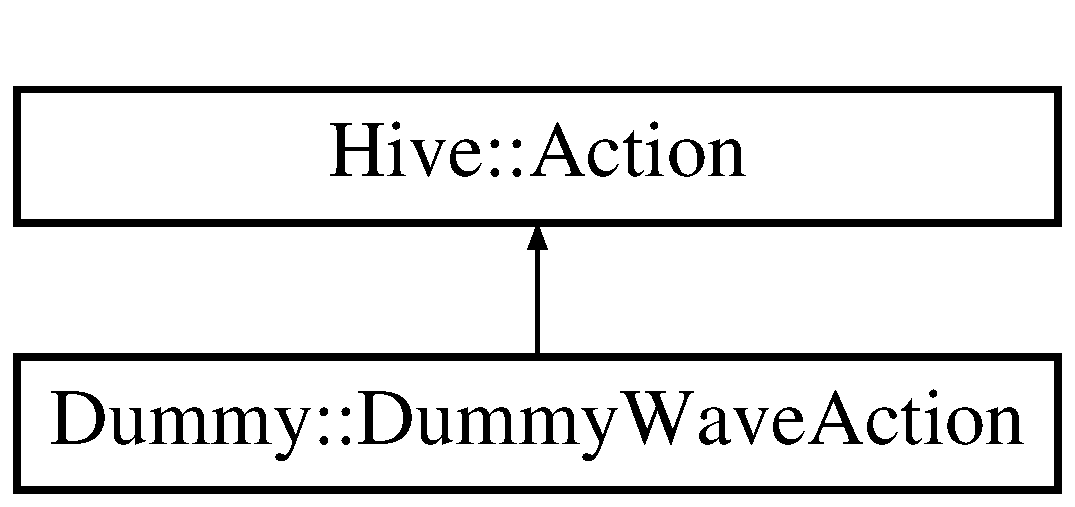
\includegraphics[height=2cm]{classHive_1_1Action}
\end{center}
\end{figure}


\subsection{Detailed Description}
action class for working on an agent 

actions are standardised methods that manipulate the dataset of an agent. a message tells the agent to perform an action.

\begin{Desc}
\item[See also:]message\end{Desc}
\begin{Desc}
\item[{\bf Todo}]everything\end{Desc}
\begin{Desc}
\item[{\bf Bug}]\end{Desc}
\begin{Desc}
\item[Author:]Garrit Jentsch\end{Desc}
\begin{Desc}
\item[Date:]Oct 13th, 2009 last edited: Oct 14th, 2009 by Garrit and Michael \end{Desc}
\subsection*{Public Member Functions}
\begin{CompactItemize}
\item 
{\bf Action} ()
\begin{CompactList}\small\item\em default constructor \item\end{CompactList}\item 
{\bf Action} (int i)
\item 
virtual {\bf $\sim$Action} ()
\begin{CompactList}\small\item\em destructor \item\end{CompactList}\item 
void {\bf setAgent} ({\bf Agent} $\ast$ag)
\item 
void {\bf setIdentifyer} (int id)
\item 
virtual void {\bf fire} ({\bf Data} $\ast$d)=0
\end{CompactItemize}
\subsection*{Protected Attributes}
\begin{CompactItemize}
\item 
int {\bf unique\_\-identifyer}
\begin{CompactList}\small\item\em identifyer of an action \item\end{CompactList}\item 
{\bf Agent} $\ast$ {\bf agent}
\begin{CompactList}\small\item\em pointer to agent on which action works \item\end{CompactList}\end{CompactItemize}


\subsection{Constructor \& Destructor Documentation}
\index{Hive::Action@{Hive::Action}!Action@{Action}}
\index{Action@{Action}!Hive::Action@{Hive::Action}}
\subsubsection[Action]{\setlength{\rightskip}{0pt plus 5cm}Hive::Action::Action ()\hspace{0.3cm}{\tt  [inline]}}\label{classHive_1_1Action_186eec9d79cb86c0f95e912df10c978c}


default constructor 

\index{Hive::Action@{Hive::Action}!Action@{Action}}
\index{Action@{Action}!Hive::Action@{Hive::Action}}
\subsubsection[Action]{\setlength{\rightskip}{0pt plus 5cm}Hive::Action::Action (int {\em i})\hspace{0.3cm}{\tt  [inline]}}\label{classHive_1_1Action_711105071e0782907a7045fe33c04f66}


constructor \begin{Desc}
\item[Parameters:]
\begin{description}
\item[{\em i}]unique\_\-identifyer \end{description}
\end{Desc}


References unique\_\-identifyer.\index{Hive::Action@{Hive::Action}!$\sim$Action@{$\sim$Action}}
\index{$\sim$Action@{$\sim$Action}!Hive::Action@{Hive::Action}}
\subsubsection[$\sim$Action]{\setlength{\rightskip}{0pt plus 5cm}virtual Hive::Action::$\sim$Action ()\hspace{0.3cm}{\tt  [inline, virtual]}}\label{classHive_1_1Action_6d175e35e5d7994ac93762da91e75e23}


destructor 



\subsection{Member Function Documentation}
\index{Hive::Action@{Hive::Action}!setAgent@{setAgent}}
\index{setAgent@{setAgent}!Hive::Action@{Hive::Action}}
\subsubsection[setAgent]{\setlength{\rightskip}{0pt plus 5cm}void Hive::Action::setAgent ({\bf Agent} $\ast$ {\em ag})\hspace{0.3cm}{\tt  [inline]}}\label{classHive_1_1Action_afc4610e9c8d64507bffc431fa7cae92}


set agent on which this action is supposed to work. \begin{Desc}
\item[Parameters:]
\begin{description}
\item[{\em $\ast$ag}]pointer to agent \end{description}
\end{Desc}


References agent.

Referenced by Dummy::DummyAgentFactory::createAgent().\index{Hive::Action@{Hive::Action}!setIdentifyer@{setIdentifyer}}
\index{setIdentifyer@{setIdentifyer}!Hive::Action@{Hive::Action}}
\subsubsection[setIdentifyer]{\setlength{\rightskip}{0pt plus 5cm}void Hive::Action::setIdentifyer (int {\em id})\hspace{0.3cm}{\tt  [inline]}}\label{classHive_1_1Action_3dba59edbabb8bebcf5c2a0ab5e54bd9}


sets identifyer of this action \begin{Desc}
\item[Parameters:]
\begin{description}
\item[{\em id}]identifyer \end{description}
\end{Desc}


References unique\_\-identifyer.\index{Hive::Action@{Hive::Action}!fire@{fire}}
\index{fire@{fire}!Hive::Action@{Hive::Action}}
\subsubsection[fire]{\setlength{\rightskip}{0pt plus 5cm}virtual void Hive::Action::fire ({\bf Data} $\ast$ {\em d})\hspace{0.3cm}{\tt  [pure virtual]}}\label{classHive_1_1Action_b49f6239755b61cd057b7024d739e8ba}


executes an action \begin{Desc}
\item[Parameters:]
\begin{description}
\item[{\em d}]pointer to data-object containing the argument for the action \end{description}
\end{Desc}


Implemented in {\bf Dummy::DummyWaveAction} \doxyref{}{p.}{classDummy_1_1DummyWaveAction_da12711cb5d2ff3f5df637dbb28ebeff}.

\subsection{Member Data Documentation}
\index{Hive::Action@{Hive::Action}!unique\_\-identifyer@{unique\_\-identifyer}}
\index{unique\_\-identifyer@{unique\_\-identifyer}!Hive::Action@{Hive::Action}}
\subsubsection[unique\_\-identifyer]{\setlength{\rightskip}{0pt plus 5cm}int {\bf Hive::Action::unique\_\-identifyer}\hspace{0.3cm}{\tt  [protected]}}\label{classHive_1_1Action_d2ee5504f3d7d4bc94cf307f5c7f6ade}


identifyer of an action 



Referenced by Action(), and setIdentifyer().\index{Hive::Action@{Hive::Action}!agent@{agent}}
\index{agent@{agent}!Hive::Action@{Hive::Action}}
\subsubsection[agent]{\setlength{\rightskip}{0pt plus 5cm}{\bf Agent}$\ast$ {\bf Hive::Action::agent}\hspace{0.3cm}{\tt  [protected]}}\label{classHive_1_1Action_5a1e64f8c572388812b9214057d96ad7}


pointer to agent on which action works 



Referenced by Dummy::DummyWaveAction::fire(), and setAgent().

The documentation for this class was generated from the following file:\begin{CompactItemize}
\item 
{\bf arnie.hh}\end{CompactItemize}

\section{Hive::Agent Class Reference}
\label{classHive_1_1Agent}\index{Hive::Agent@{Hive::Agent}}
{\tt \#include $<$agent.hh$>$}



\subsection{Detailed Description}
central class of the hive 

the agent is the central class of the hive. an agent contains a database in which it stores its knowledge. its simulators operate on the data stored within the database. communication among agents is accomplished with the communicator. when agents communicate they place messages on to the message queue of another agent. a message tells the agent to perform an action from its actionset.

\begin{Desc}
\item[{\bf Todo}]Everything\end{Desc}
\begin{Desc}
\item[{\bf Bug}]\end{Desc}
\begin{Desc}
\item[Author:]Garrit Jentsch\end{Desc}
\begin{Desc}
\item[Date:]Oct 12th, 2009 last edited: Oct 14h, 2009 by Garrit and Michael \end{Desc}
\subsection*{Public Member Functions}
\begin{CompactItemize}
\item 
{\bf Agent} ()
\begin{CompactList}\small\item\em constructor \item\end{CompactList}\item 
{\bf Agent} (int {\bf agent\_\-id})
\item 
{\bf $\sim$Agent} ()
\begin{CompactList}\small\item\em destructor \item\end{CompactList}\item 
void {\bf setParent} (int {\bf parent\_\-id})
\item 
void {\bf addChild} (int child\_\-id)
\item 
void {\bf addAction} ({\bf Action} $\ast$a)
\item 
void {\bf addCommunicator} ({\bf Communicator} $\ast${\bf c})
\item 
void {\bf addMessageGenerator} ({\bf MessageGenerator} $\ast$msg)
\item 
void {\bf addSimulator} ({\bf Simulator} $\ast$s)
\item 
{\bf Database} $\ast$ {\bf getDatabase} ()
\item 
int {\bf getParentId} ()
\item 
int {\bf getAgentId} ()
\item 
int {\bf getNumOfChildren} ()
\item 
int {\bf getChildAgentId} (int childIndex)
\item 
bool {\bf isChildAgent} (int agentId)
\item 
void {\bf outputCurrentState} ({\bf OutputWriter} $\ast$ow)
\item 
void {\bf placeMessageOnMessageQueue} ({\bf Message} $\ast$m)
\item 
void {\bf propagate} (double time)
\begin{CompactList}\small\item\em propagates the agent for a timestep \item\end{CompactList}\item 
void {\bf setupDatabase} ()
\end{CompactItemize}
\subsection*{Protected Member Functions}
\begin{CompactItemize}
\item 
void {\bf evaluateMessageQueue} ()
\begin{CompactList}\small\item\em causes the agent to perform the actions placed on the message queue. \item\end{CompactList}\end{CompactItemize}
\subsection*{Protected Attributes}
\begin{CompactItemize}
\item 
int {\bf agent\_\-id}
\begin{CompactList}\small\item\em unique identifyer of this agent \item\end{CompactList}\item 
int {\bf parent\_\-id}
\begin{CompactList}\small\item\em unique identifyer of the parent agent \item\end{CompactList}\item 
vector$<$ int $>$ {\bf children\_\-id}
\begin{CompactList}\small\item\em unique identifyers of the child agents \item\end{CompactList}\item 
{\bf Database} $\ast$ {\bf db}
\begin{CompactList}\small\item\em database of the agent \item\end{CompactList}\item 
{\bf Communicator} $\ast$ {\bf c}
\begin{CompactList}\small\item\em communicator for exchanging messages with the agent's parent agent andchildren \item\end{CompactList}\item 
queue$<$ {\bf Message} $\ast$ $>$ {\bf message\_\-queue}
\begin{CompactList}\small\item\em message queue; inbox of an agent \item\end{CompactList}\item 
vector$<$ {\bf Simulator} $\ast$ $>$ {\bf simulators}
\begin{CompactList}\small\item\em vector of simulators \item\end{CompactList}\item 
vector$<$ {\bf Action} $\ast$ $>$ {\bf action\_\-set}
\begin{CompactList}\small\item\em actionset. a message tells the agent to execute an action from this set \item\end{CompactList}\item 
vector$<$ {\bf Message} $\ast$ $>$ {\bf outbox}
\begin{CompactList}\small\item\em message outbox of agent. \item\end{CompactList}\item 
vector$<$ {\bf MessageGenerator} $\ast$ $>$ {\bf message\_\-generators}
\begin{CompactList}\small\item\em vector of pointers to message\_\-generators \item\end{CompactList}\end{CompactItemize}


\subsection{Constructor \& Destructor Documentation}
\index{Hive::Agent@{Hive::Agent}!Agent@{Agent}}
\index{Agent@{Agent}!Hive::Agent@{Hive::Agent}}
\subsubsection[Agent]{\setlength{\rightskip}{0pt plus 5cm}Agent::Agent ()}\label{classHive_1_1Agent_24a60f1d260bf19a4f7f8a5f36881d3f}


constructor 



unique identifyer of this agent

database of the agent

communicator for exchanging messages with the agent's parent agent andchildren

message queue; inbox of an agent

vector of simulators

actionset. a message tells the agent to execute an action from this set

message outbox of agent.

vector of pointers to message\_\-generators 

References agent\_\-id, db, and parent\_\-id.\index{Hive::Agent@{Hive::Agent}!Agent@{Agent}}
\index{Agent@{Agent}!Hive::Agent@{Hive::Agent}}
\subsubsection[Agent]{\setlength{\rightskip}{0pt plus 5cm}Agent::Agent (int {\em agent\_\-id})}\label{classHive_1_1Agent_9bdb60eaf7b1967cb0e77665af1d0d4e}




References db.\index{Hive::Agent@{Hive::Agent}!$\sim$Agent@{$\sim$Agent}}
\index{$\sim$Agent@{$\sim$Agent}!Hive::Agent@{Hive::Agent}}
\subsubsection[$\sim$Agent]{\setlength{\rightskip}{0pt plus 5cm}Agent::$\sim$Agent ()}\label{classHive_1_1Agent_b8dd8d152605cf1339fed595376e83cb}


destructor 



References agent\_\-id.

\subsection{Member Function Documentation}
\index{Hive::Agent@{Hive::Agent}!setParent@{setParent}}
\index{setParent@{setParent}!Hive::Agent@{Hive::Agent}}
\subsubsection[setParent]{\setlength{\rightskip}{0pt plus 5cm}void Agent::setParent (int {\em parent\_\-id})}\label{classHive_1_1Agent_a6731cfdbcd8fd882e3f49a93c73dad8}


set the parent of this agent \begin{Desc}
\item[Parameters:]
\begin{description}
\item[{\em parent\_\-id}]id of the parent \end{description}
\end{Desc}
\index{Hive::Agent@{Hive::Agent}!addChild@{addChild}}
\index{addChild@{addChild}!Hive::Agent@{Hive::Agent}}
\subsubsection[addChild]{\setlength{\rightskip}{0pt plus 5cm}void Agent::addChild (int {\em child\_\-id})}\label{classHive_1_1Agent_9635010b401c5249d974a8a071d49261}


add a child of this agent \begin{Desc}
\item[Parameters:]
\begin{description}
\item[{\em child\_\-id}]id of child to add \end{description}
\end{Desc}


References children\_\-id.\index{Hive::Agent@{Hive::Agent}!addAction@{addAction}}
\index{addAction@{addAction}!Hive::Agent@{Hive::Agent}}
\subsubsection[addAction]{\setlength{\rightskip}{0pt plus 5cm}void Agent::addAction ({\bf Action} $\ast$ {\em a})}\label{classHive_1_1Agent_f03cb3281f45d966a5df796d9922e955}


adds an action to the actionset \begin{Desc}
\item[Parameters:]
\begin{description}
\item[{\em a}]action to be added to actionset \end{description}
\end{Desc}


References action\_\-set.

Referenced by Dummy::DummyAgentFactory::createAgent().\index{Hive::Agent@{Hive::Agent}!addCommunicator@{addCommunicator}}
\index{addCommunicator@{addCommunicator}!Hive::Agent@{Hive::Agent}}
\subsubsection[addCommunicator]{\setlength{\rightskip}{0pt plus 5cm}void Agent::addCommunicator ({\bf Communicator} $\ast$ {\em c})}\label{classHive_1_1Agent_4d1723cd30329f5da052fee0dc6fa5ef}


adds communicator to the system \begin{Desc}
\item[Parameters:]
\begin{description}
\item[{\em c}]communicator to be added \end{description}
\end{Desc}
\index{Hive::Agent@{Hive::Agent}!addMessageGenerator@{addMessageGenerator}}
\index{addMessageGenerator@{addMessageGenerator}!Hive::Agent@{Hive::Agent}}
\subsubsection[addMessageGenerator]{\setlength{\rightskip}{0pt plus 5cm}void Agent::addMessageGenerator ({\bf MessageGenerator} $\ast$ {\em msg})}\label{classHive_1_1Agent_f2414a0dacdc08419a4cc1b2c5d0276f}


adds a message generator to the agent \begin{Desc}
\item[Parameters:]
\begin{description}
\item[{\em msg}]messagegenerator \end{description}
\end{Desc}


References message\_\-generators.

Referenced by Dummy::DummyAgentFactory::createAgent().\index{Hive::Agent@{Hive::Agent}!addSimulator@{addSimulator}}
\index{addSimulator@{addSimulator}!Hive::Agent@{Hive::Agent}}
\subsubsection[addSimulator]{\setlength{\rightskip}{0pt plus 5cm}void Agent::addSimulator ({\bf Simulator} $\ast$ {\em s})}\label{classHive_1_1Agent_5c0b83894065bd48801026269297c7d4}


adds a simulator to the simulators vector \begin{Desc}
\item[Parameters:]
\begin{description}
\item[{\em s}]simulator to be added \end{description}
\end{Desc}


References simulators.

Referenced by Dummy::DummyAgentFactory::createAgent().\index{Hive::Agent@{Hive::Agent}!getDatabase@{getDatabase}}
\index{getDatabase@{getDatabase}!Hive::Agent@{Hive::Agent}}
\subsubsection[getDatabase]{\setlength{\rightskip}{0pt plus 5cm}{\bf Hive::Database} $\ast$ Agent::getDatabase ()}\label{classHive_1_1Agent_a2e9e670185a1cc43c392dd3d3450bca}


method for accessing database of an agent \begin{Desc}
\item[Returns:]pointer to database \end{Desc}


References db.

Referenced by Dummy::DummyAgentFactory::createAgent(), Hive::DummySimulator::DummySimulator(), and Dummy::DummyWaveAction::fire().\index{Hive::Agent@{Hive::Agent}!getParentId@{getParentId}}
\index{getParentId@{getParentId}!Hive::Agent@{Hive::Agent}}
\subsubsection[getParentId]{\setlength{\rightskip}{0pt plus 5cm}int Agent::getParentId ()}\label{classHive_1_1Agent_bf305ea102ca79f0619e4ee30b856868}


return parent agent ID \begin{Desc}
\item[Returns:]ID of the parent agent \end{Desc}


References parent\_\-id.\index{Hive::Agent@{Hive::Agent}!getAgentId@{getAgentId}}
\index{getAgentId@{getAgentId}!Hive::Agent@{Hive::Agent}}
\subsubsection[getAgentId]{\setlength{\rightskip}{0pt plus 5cm}int Agent::getAgentId ()}\label{classHive_1_1Agent_3b6ebc7294216a2f8e7e0d4cbfdfd33b}


return this agent ID \begin{Desc}
\item[Returns:]ID of the parent agent \end{Desc}


References agent\_\-id.

Referenced by Hive::SerialCommunicator::addAgent(), Hive::DummySimulator::prepare(), and Hive::DummySimulator::synchroniseWithDatabase().\index{Hive::Agent@{Hive::Agent}!getNumOfChildren@{getNumOfChildren}}
\index{getNumOfChildren@{getNumOfChildren}!Hive::Agent@{Hive::Agent}}
\subsubsection[getNumOfChildren]{\setlength{\rightskip}{0pt plus 5cm}int Agent::getNumOfChildren ()}\label{classHive_1_1Agent_9b67da3082d21e119943e0ff43642b56}


get the number of child agents \begin{Desc}
\item[Returns:]the number of children \end{Desc}


References children\_\-id.\index{Hive::Agent@{Hive::Agent}!getChildAgentId@{getChildAgentId}}
\index{getChildAgentId@{getChildAgentId}!Hive::Agent@{Hive::Agent}}
\subsubsection[getChildAgentId]{\setlength{\rightskip}{0pt plus 5cm}int Agent::getChildAgentId (int {\em childIndex})}\label{classHive_1_1Agent_7ad69e92da1d4dcee56680f3da3aba66}


return the ID of the child agent at the given index \begin{Desc}
\item[Parameters:]
\begin{description}
\item[{\em childIndex}]index of the child agent ID to return \end{description}
\end{Desc}


References children\_\-id.\index{Hive::Agent@{Hive::Agent}!isChildAgent@{isChildAgent}}
\index{isChildAgent@{isChildAgent}!Hive::Agent@{Hive::Agent}}
\subsubsection[isChildAgent]{\setlength{\rightskip}{0pt plus 5cm}bool Agent::isChildAgent (int {\em agentId})}\label{classHive_1_1Agent_d9f2480125d9382dbde4b59cbeeb2f5b}


check if the given ID is a child of this \begin{Desc}
\item[Returns:]true if the agentID given is a child, false otherwise childIndex index of the child agent ID to return \end{Desc}


References children\_\-id.\index{Hive::Agent@{Hive::Agent}!outputCurrentState@{outputCurrentState}}
\index{outputCurrentState@{outputCurrentState}!Hive::Agent@{Hive::Agent}}
\subsubsection[outputCurrentState]{\setlength{\rightskip}{0pt plus 5cm}void Agent::outputCurrentState ({\bf OutputWriter} $\ast$ {\em ow})}\label{classHive_1_1Agent_6904cc83add9827300b9830e45239abc}


outputs the current state of the agent by dumbing its database \begin{Desc}
\item[Parameters:]
\begin{description}
\item[{\em ow}]pointer to outputwriter who does the actual job \end{description}
\end{Desc}


References agent\_\-id.\index{Hive::Agent@{Hive::Agent}!placeMessageOnMessageQueue@{placeMessageOnMessageQueue}}
\index{placeMessageOnMessageQueue@{placeMessageOnMessageQueue}!Hive::Agent@{Hive::Agent}}
\subsubsection[placeMessageOnMessageQueue]{\setlength{\rightskip}{0pt plus 5cm}void Hive::Agent::placeMessageOnMessageQueue ({\bf Message} $\ast$ {\em m})\hspace{0.3cm}{\tt  [inline]}}\label{classHive_1_1Agent_8d977f6dd7877a04da48c9325e89fada}




References message\_\-queue.

Referenced by Dummy::DummyMessageGenerator::placeMessage().\index{Hive::Agent@{Hive::Agent}!propagate@{propagate}}
\index{propagate@{propagate}!Hive::Agent@{Hive::Agent}}
\subsubsection[propagate]{\setlength{\rightskip}{0pt plus 5cm}void Agent::propagate (double {\em time})}\label{classHive_1_1Agent_6eb011086d7ad1640a466affe952b78f}


propagates the agent for a timestep 



References agent\_\-id, c, children\_\-id, evaluateMessageQueue(), message\_\-generators, outbox, Hive::Communicator::propogateAgent(), Hive::Communicator::sendMessage(), and simulators.

Referenced by main().\index{Hive::Agent@{Hive::Agent}!setupDatabase@{setupDatabase}}
\index{setupDatabase@{setupDatabase}!Hive::Agent@{Hive::Agent}}
\subsubsection[setupDatabase]{\setlength{\rightskip}{0pt plus 5cm}void Agent::setupDatabase ()}\label{classHive_1_1Agent_0bf4d254bc310eb8eb9ea16b50571ee3}


method for initializing the database. again the actual job is being done by the database-initializer \begin{Desc}
\item[Parameters:]
\begin{description}
\item[{\em $\ast$db\_\-init}]pointer to database initializer \end{description}
\end{Desc}


References agent\_\-id.\index{Hive::Agent@{Hive::Agent}!evaluateMessageQueue@{evaluateMessageQueue}}
\index{evaluateMessageQueue@{evaluateMessageQueue}!Hive::Agent@{Hive::Agent}}
\subsubsection[evaluateMessageQueue]{\setlength{\rightskip}{0pt plus 5cm}void Agent::evaluateMessageQueue ()\hspace{0.3cm}{\tt  [protected]}}\label{classHive_1_1Agent_1da352e749752c141c4b3c4566c2023d}


causes the agent to perform the actions placed on the message queue. 



References action\_\-set, agent\_\-id, Hive::Message::getActionId(), Hive::Message::getArgument(), and message\_\-queue.

Referenced by propagate().

\subsection{Member Data Documentation}
\index{Hive::Agent@{Hive::Agent}!agent\_\-id@{agent\_\-id}}
\index{agent\_\-id@{agent\_\-id}!Hive::Agent@{Hive::Agent}}
\subsubsection[agent\_\-id]{\setlength{\rightskip}{0pt plus 5cm}int {\bf Hive::Agent::agent\_\-id}\hspace{0.3cm}{\tt  [protected]}}\label{classHive_1_1Agent_91c9681062f0b75a8f3cc38a8752f2c4}


unique identifyer of this agent 



Referenced by Agent(), evaluateMessageQueue(), getAgentId(), outputCurrentState(), propagate(), setupDatabase(), and $\sim$Agent().\index{Hive::Agent@{Hive::Agent}!parent\_\-id@{parent\_\-id}}
\index{parent\_\-id@{parent\_\-id}!Hive::Agent@{Hive::Agent}}
\subsubsection[parent\_\-id]{\setlength{\rightskip}{0pt plus 5cm}int {\bf Hive::Agent::parent\_\-id}\hspace{0.3cm}{\tt  [protected]}}\label{classHive_1_1Agent_b6ab3584f5ff74d9a8c498cd4a26a491}


unique identifyer of the parent agent 



Referenced by Agent(), and getParentId().\index{Hive::Agent@{Hive::Agent}!children\_\-id@{children\_\-id}}
\index{children\_\-id@{children\_\-id}!Hive::Agent@{Hive::Agent}}
\subsubsection[children\_\-id]{\setlength{\rightskip}{0pt plus 5cm}vector$<$int$>$ {\bf Hive::Agent::children\_\-id}\hspace{0.3cm}{\tt  [protected]}}\label{classHive_1_1Agent_a9b335d3bd4a0040931ec8a91741ea53}


unique identifyers of the child agents 



Referenced by addChild(), getChildAgentId(), getNumOfChildren(), isChildAgent(), and propagate().\index{Hive::Agent@{Hive::Agent}!db@{db}}
\index{db@{db}!Hive::Agent@{Hive::Agent}}
\subsubsection[db]{\setlength{\rightskip}{0pt plus 5cm}{\bf Database}$\ast$ {\bf Hive::Agent::db}\hspace{0.3cm}{\tt  [protected]}}\label{classHive_1_1Agent_4b74705c85d99d50c455e09f69ba01b3}


database of the agent 



Referenced by Agent(), and getDatabase().\index{Hive::Agent@{Hive::Agent}!c@{c}}
\index{c@{c}!Hive::Agent@{Hive::Agent}}
\subsubsection[c]{\setlength{\rightskip}{0pt plus 5cm}{\bf Communicator}$\ast$ {\bf Hive::Agent::c}\hspace{0.3cm}{\tt  [protected]}}\label{classHive_1_1Agent_e33ddbcb078d89fd49914966e1c2edff}


communicator for exchanging messages with the agent's parent agent andchildren 



Referenced by propagate().\index{Hive::Agent@{Hive::Agent}!message\_\-queue@{message\_\-queue}}
\index{message\_\-queue@{message\_\-queue}!Hive::Agent@{Hive::Agent}}
\subsubsection[message\_\-queue]{\setlength{\rightskip}{0pt plus 5cm}queue$<${\bf Message}$\ast$ $>$ {\bf Hive::Agent::message\_\-queue}\hspace{0.3cm}{\tt  [protected]}}\label{classHive_1_1Agent_e9ad453f7e0d71252685f5b20ab268dd}


message queue; inbox of an agent 



Referenced by evaluateMessageQueue(), and placeMessageOnMessageQueue().\index{Hive::Agent@{Hive::Agent}!simulators@{simulators}}
\index{simulators@{simulators}!Hive::Agent@{Hive::Agent}}
\subsubsection[simulators]{\setlength{\rightskip}{0pt plus 5cm}vector$<${\bf Simulator} $\ast$$>$ {\bf Hive::Agent::simulators}\hspace{0.3cm}{\tt  [protected]}}\label{classHive_1_1Agent_ffc50f2e6b27ea7af8525f9f080e89c9}


vector of simulators 



Referenced by addSimulator(), and propagate().\index{Hive::Agent@{Hive::Agent}!action\_\-set@{action\_\-set}}
\index{action\_\-set@{action\_\-set}!Hive::Agent@{Hive::Agent}}
\subsubsection[action\_\-set]{\setlength{\rightskip}{0pt plus 5cm}vector$<${\bf Action} $\ast$$>$ {\bf Hive::Agent::action\_\-set}\hspace{0.3cm}{\tt  [protected]}}\label{classHive_1_1Agent_03600d794b244ad8aeb88507f74a9370}


actionset. a message tells the agent to execute an action from this set 



Referenced by addAction(), and evaluateMessageQueue().\index{Hive::Agent@{Hive::Agent}!outbox@{outbox}}
\index{outbox@{outbox}!Hive::Agent@{Hive::Agent}}
\subsubsection[outbox]{\setlength{\rightskip}{0pt plus 5cm}vector$<${\bf Message} $\ast$$>$ {\bf Hive::Agent::outbox}\hspace{0.3cm}{\tt  [protected]}}\label{classHive_1_1Agent_50264a5ea66534167831275f7d6e819b}


message outbox of agent. 



Referenced by propagate().\index{Hive::Agent@{Hive::Agent}!message\_\-generators@{message\_\-generators}}
\index{message\_\-generators@{message\_\-generators}!Hive::Agent@{Hive::Agent}}
\subsubsection[message\_\-generators]{\setlength{\rightskip}{0pt plus 5cm}vector$<${\bf MessageGenerator}$\ast$ $>$ {\bf Hive::Agent::message\_\-generators}\hspace{0.3cm}{\tt  [protected]}}\label{classHive_1_1Agent_416f0406ae78863aa45d4fbfd570ad68}


vector of pointers to message\_\-generators 



Referenced by addMessageGenerator(), and propagate().

The documentation for this class was generated from the following files:\begin{CompactItemize}
\item 
{\bf agent.hh}\item 
{\bf agent.cpp}\end{CompactItemize}

\section{Hive::AgentFactory Class Reference}
\label{classHive_1_1AgentFactory}\index{Hive::AgentFactory@{Hive::AgentFactory}}
{\tt \#include $<$agent\_\-factory.hh$>$}

Inheritance diagram for Hive::AgentFactory::\begin{figure}[H]
\begin{center}
\leavevmode
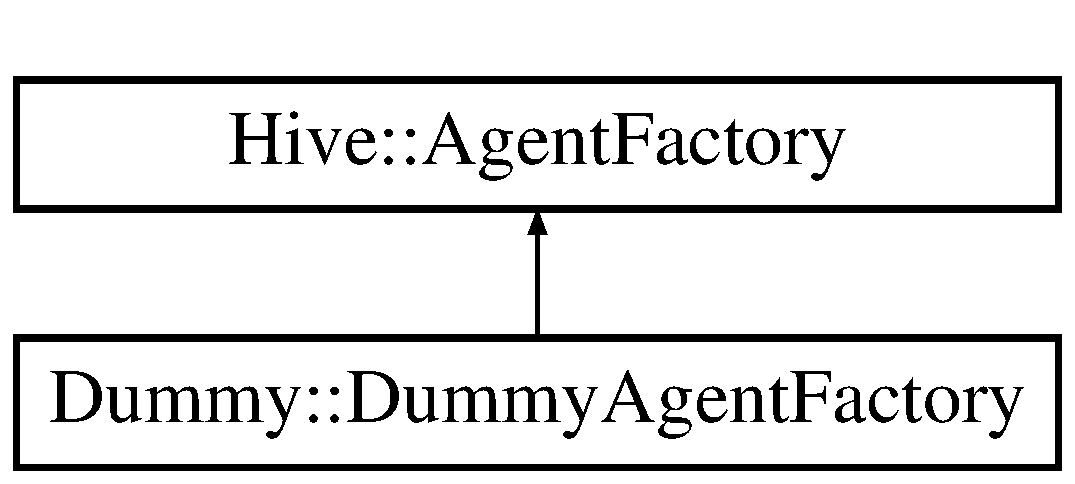
\includegraphics[height=2cm]{classHive_1_1AgentFactory}
\end{center}
\end{figure}


\subsection{Detailed Description}
agent factory 

agent factory for constructing agents.

\begin{Desc}
\item[{\bf Todo}]Everything\end{Desc}
\begin{Desc}
\item[{\bf Bug}]who know's?\end{Desc}
\begin{Desc}
\item[Author:]Garrit Jentsch\end{Desc}
\begin{Desc}
\item[Date:]13th of October, 2009 last edited: 10-14-2009 by Garrit and Michael \end{Desc}
\subsection*{Public Member Functions}
\begin{CompactItemize}
\item 
{\bf AgentFactory} ()
\begin{CompactList}\small\item\em default constructor \item\end{CompactList}\item 
{\bf AgentFactory} ({\bf InputSystemReader} $\ast${\bf isr})
\item 
virtual {\bf $\sim$AgentFactory} ()
\begin{CompactList}\small\item\em destructor \item\end{CompactList}\item 
virtual {\bf Agent} $\ast$ {\bf createAgent} ()=0
\item 
virtual {\bf Agent} $\ast$ {\bf createAgent} ({\bf Action} $\ast$$\ast$as)=0
\item 
virtual {\bf Agent} $\ast$ {\bf duplicateAgent} ({\bf Agent} $\ast$ag)=0
\item 
void {\bf setInputSystemReader} ({\bf InputSystemReader} $\ast${\bf isr})
\end{CompactItemize}
\subsection*{Protected Member Functions}
\begin{CompactItemize}
\item 
virtual void {\bf addActionToAgentsActionSet} ({\bf Action} $\ast$a)=0
\item 
virtual void {\bf addSimulatorToAgent} ({\bf Simulator} $\ast$s)=0
\end{CompactItemize}
\subsection*{Protected Attributes}
\begin{CompactItemize}
\item 
{\bf System} $\ast$ {\bf sys}
\begin{CompactList}\small\item\em system \item\end{CompactList}\item 
{\bf InputSystemReader} $\ast$ {\bf isr}
\begin{CompactList}\small\item\em input\_\-reader \item\end{CompactList}\end{CompactItemize}


\subsection{Constructor \& Destructor Documentation}
\index{Hive::AgentFactory@{Hive::AgentFactory}!AgentFactory@{AgentFactory}}
\index{AgentFactory@{AgentFactory}!Hive::AgentFactory@{Hive::AgentFactory}}
\subsubsection[AgentFactory]{\setlength{\rightskip}{0pt plus 5cm}Hive::AgentFactory::AgentFactory ()\hspace{0.3cm}{\tt  [inline]}}\label{classHive_1_1AgentFactory_60004ca9ecbad370b569cae207b55c61}


default constructor 

\index{Hive::AgentFactory@{Hive::AgentFactory}!AgentFactory@{AgentFactory}}
\index{AgentFactory@{AgentFactory}!Hive::AgentFactory@{Hive::AgentFactory}}
\subsubsection[AgentFactory]{\setlength{\rightskip}{0pt plus 5cm}Hive::AgentFactory::AgentFactory ({\bf InputSystemReader} $\ast$ {\em isr})\hspace{0.3cm}{\tt  [inline]}}\label{classHive_1_1AgentFactory_9db85c48d7daa60900f42384b0627560}


constructor \begin{Desc}
\item[Parameters:]
\begin{description}
\item[{\em $\ast$isr}]pointer to inputsystemreader \end{description}
\end{Desc}
\index{Hive::AgentFactory@{Hive::AgentFactory}!$\sim$AgentFactory@{$\sim$AgentFactory}}
\index{$\sim$AgentFactory@{$\sim$AgentFactory}!Hive::AgentFactory@{Hive::AgentFactory}}
\subsubsection[$\sim$AgentFactory]{\setlength{\rightskip}{0pt plus 5cm}virtual Hive::AgentFactory::$\sim$AgentFactory ()\hspace{0.3cm}{\tt  [inline, virtual]}}\label{classHive_1_1AgentFactory_72d8240038c2669ba66797654640be29}


destructor 



\subsection{Member Function Documentation}
\index{Hive::AgentFactory@{Hive::AgentFactory}!createAgent@{createAgent}}
\index{createAgent@{createAgent}!Hive::AgentFactory@{Hive::AgentFactory}}
\subsubsection[createAgent]{\setlength{\rightskip}{0pt plus 5cm}virtual {\bf Agent}$\ast$ Hive::AgentFactory::createAgent ()\hspace{0.3cm}{\tt  [pure virtual]}}\label{classHive_1_1AgentFactory_a1e148a842b3f0e2dd11de0ef61bf877}


create agent of a certain type. encapsulates everything that has to be done, i.e. it adds actions, simulator, messagegenerators, and communicator to the agent. the simulator is also told to connect to the database and initialize itself. \begin{Desc}
\item[Returns:]pointer to constructed agent \end{Desc}


Implemented in {\bf Dummy::DummyAgentFactory} \doxyref{}{p.}{classDummy_1_1DummyAgentFactory_0aec7238d1758a98d59817f49ae1c2c0}.

Referenced by Dummy::DummyComposer::createAgent().\index{Hive::AgentFactory@{Hive::AgentFactory}!createAgent@{createAgent}}
\index{createAgent@{createAgent}!Hive::AgentFactory@{Hive::AgentFactory}}
\subsubsection[createAgent]{\setlength{\rightskip}{0pt plus 5cm}virtual {\bf Agent}$\ast$ Hive::AgentFactory::createAgent ({\bf Action} $\ast$$\ast$ {\em as})\hspace{0.3cm}{\tt  [pure virtual]}}\label{classHive_1_1AgentFactory_40e828a8b7c397c11a3c0ed24e22932d}


create an agent and provide actionset as an argument \begin{Desc}
\item[Parameters:]
\begin{description}
\item[{\em as}]pointer to actionset \end{description}
\end{Desc}


Implemented in {\bf Dummy::DummyAgentFactory} \doxyref{}{p.}{classDummy_1_1DummyAgentFactory_939e7c2ccee8945187801e6cd92da0df}.\index{Hive::AgentFactory@{Hive::AgentFactory}!duplicateAgent@{duplicateAgent}}
\index{duplicateAgent@{duplicateAgent}!Hive::AgentFactory@{Hive::AgentFactory}}
\subsubsection[duplicateAgent]{\setlength{\rightskip}{0pt plus 5cm}virtual {\bf Agent}$\ast$ Hive::AgentFactory::duplicateAgent ({\bf Agent} $\ast$ {\em ag})\hspace{0.3cm}{\tt  [pure virtual]}}\label{classHive_1_1AgentFactory_ea99bc08ec4fa2a262244362e7de03f6}


copies an agent \begin{Desc}
\item[Parameters:]
\begin{description}
\item[{\em $\ast$ag}]pointer to agent to be copied \end{description}
\end{Desc}
\begin{Desc}
\item[Returns:]pointer to copy \end{Desc}


Implemented in {\bf Dummy::DummyAgentFactory} \doxyref{}{p.}{classDummy_1_1DummyAgentFactory_8ddeb4e5090dac67d921e8a4b89275a7}.\index{Hive::AgentFactory@{Hive::AgentFactory}!setInputSystemReader@{setInputSystemReader}}
\index{setInputSystemReader@{setInputSystemReader}!Hive::AgentFactory@{Hive::AgentFactory}}
\subsubsection[setInputSystemReader]{\setlength{\rightskip}{0pt plus 5cm}void Hive::AgentFactory::setInputSystemReader ({\bf InputSystemReader} $\ast$ {\em isr})\hspace{0.3cm}{\tt  [inline]}}\label{classHive_1_1AgentFactory_8f3f49944a65e04224a903f90622fcdc}


sets up inputsystemreader \begin{Desc}
\item[Parameters:]
\begin{description}
\item[{\em $\ast$isr}]inputsystemreader for this factory \end{description}
\end{Desc}
\index{Hive::AgentFactory@{Hive::AgentFactory}!addActionToAgentsActionSet@{addActionToAgentsActionSet}}
\index{addActionToAgentsActionSet@{addActionToAgentsActionSet}!Hive::AgentFactory@{Hive::AgentFactory}}
\subsubsection[addActionToAgentsActionSet]{\setlength{\rightskip}{0pt plus 5cm}virtual void Hive::AgentFactory::addActionToAgentsActionSet ({\bf Action} $\ast$ {\em a})\hspace{0.3cm}{\tt  [protected, pure virtual]}}\label{classHive_1_1AgentFactory_978d73e56c472e6ecce59282fa80852e}


adds an action to the agents action set \begin{Desc}
\item[Parameters:]
\begin{description}
\item[{\em $\ast$a}]pointer to action \end{description}
\end{Desc}


Implemented in {\bf Dummy::DummyAgentFactory} \doxyref{}{p.}{classDummy_1_1DummyAgentFactory_f469c5c34c6d26c944d9272c3bff6cb5}.\index{Hive::AgentFactory@{Hive::AgentFactory}!addSimulatorToAgent@{addSimulatorToAgent}}
\index{addSimulatorToAgent@{addSimulatorToAgent}!Hive::AgentFactory@{Hive::AgentFactory}}
\subsubsection[addSimulatorToAgent]{\setlength{\rightskip}{0pt plus 5cm}virtual void Hive::AgentFactory::addSimulatorToAgent ({\bf Simulator} $\ast$ {\em s})\hspace{0.3cm}{\tt  [protected, pure virtual]}}\label{classHive_1_1AgentFactory_e10d7f9aeb994662565de5fa7d074e87}


adds a simulator to the agents simulator set \begin{Desc}
\item[Parameters:]
\begin{description}
\item[{\em $\ast$s}]pointer to simulator \end{description}
\end{Desc}


Implemented in {\bf Dummy::DummyAgentFactory} \doxyref{}{p.}{classDummy_1_1DummyAgentFactory_52894893fc20746c63949ee62ff875af}.

\subsection{Member Data Documentation}
\index{Hive::AgentFactory@{Hive::AgentFactory}!sys@{sys}}
\index{sys@{sys}!Hive::AgentFactory@{Hive::AgentFactory}}
\subsubsection[sys]{\setlength{\rightskip}{0pt plus 5cm}{\bf System}$\ast$ {\bf Hive::AgentFactory::sys}\hspace{0.3cm}{\tt  [protected]}}\label{classHive_1_1AgentFactory_8e26672aeb4acfb444dc5cd3c0aeea01}


system 

\index{Hive::AgentFactory@{Hive::AgentFactory}!isr@{isr}}
\index{isr@{isr}!Hive::AgentFactory@{Hive::AgentFactory}}
\subsubsection[isr]{\setlength{\rightskip}{0pt plus 5cm}{\bf InputSystemReader}$\ast$ {\bf Hive::AgentFactory::isr}\hspace{0.3cm}{\tt  [protected]}}\label{classHive_1_1AgentFactory_0cc73c17d670dd1a1497a089d00a346c}


input\_\-reader 



The documentation for this class was generated from the following file:\begin{CompactItemize}
\item 
{\bf agent\_\-factory.hh}\end{CompactItemize}

\section{Hive::BoolData Class Reference}
\label{classHive_1_1BoolData}\index{Hive::BoolData@{Hive::BoolData}}
{\tt \#include $<$primitiveData.hh$>$}

Inheritance diagram for Hive::BoolData::\begin{figure}[H]
\begin{center}
\leavevmode
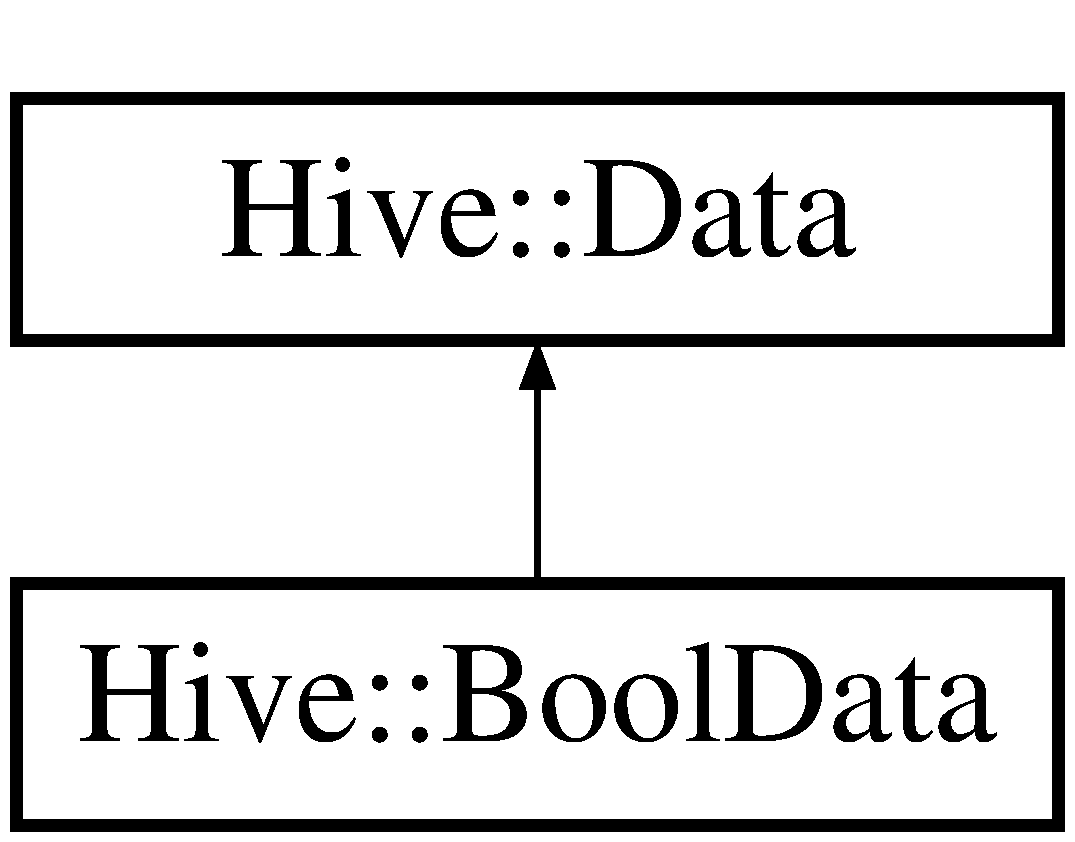
\includegraphics[height=2cm]{classHive_1_1BoolData}
\end{center}
\end{figure}


\subsection{Detailed Description}
A data object to store integer values. 

\begin{Desc}
\item[Date:]Oct 14, 2009 Last edited: Oct 14, 2009 by Garrit and Michael \end{Desc}
\begin{Desc}
\item[Author:]Michael Sneddon \end{Desc}
\subsection*{Public Member Functions}
\begin{CompactItemize}
\item 
{\bf BoolData} (string dataName, bool value)
\begin{CompactList}\small\item\em default-constructor \item\end{CompactList}\item 
virtual {\bf $\sim$BoolData} ()
\item 
void {\bf printContent} (ostream \&out)
\begin{CompactList}\small\item\em virtual method for print the content of a data item on sterr. \item\end{CompactList}\item 
string {\bf getDataName} () const 
\item 
bool {\bf getBool} () const 
\item 
void {\bf setBool} (bool newValue)
\end{CompactItemize}


\subsection{Constructor \& Destructor Documentation}
\index{Hive::BoolData@{Hive::BoolData}!BoolData@{BoolData}}
\index{BoolData@{BoolData}!Hive::BoolData@{Hive::BoolData}}
\subsubsection[BoolData]{\setlength{\rightskip}{0pt plus 5cm}BoolData::BoolData (string {\em dataName}, \/  bool {\em value})}\label{classHive_1_1BoolData_083484cf6623dd6e48c9d3f682a8a214}


default-constructor 

\index{Hive::BoolData@{Hive::BoolData}!$\sim$BoolData@{$\sim$BoolData}}
\index{$\sim$BoolData@{$\sim$BoolData}!Hive::BoolData@{Hive::BoolData}}
\subsubsection[$\sim$BoolData]{\setlength{\rightskip}{0pt plus 5cm}virtual Hive::BoolData::$\sim$BoolData ()\hspace{0.3cm}{\tt  [inline, virtual]}}\label{classHive_1_1BoolData_f1f9d2325563f9538a4afd64be7cc05f}




\subsection{Member Function Documentation}
\index{Hive::BoolData@{Hive::BoolData}!printContent@{printContent}}
\index{printContent@{printContent}!Hive::BoolData@{Hive::BoolData}}
\subsubsection[printContent]{\setlength{\rightskip}{0pt plus 5cm}void BoolData::printContent (ostream \& {\em out})\hspace{0.3cm}{\tt  [virtual]}}\label{classHive_1_1BoolData_4480d929f6baf36ac991c346e4a4b3ea}


virtual method for print the content of a data item on sterr. 



Implements {\bf Hive::Data} \doxyref{}{p.}{classHive_1_1Data_a168edcfa6efd38fe88d72c5162fd8d1}.

References Hive::Data::datatype.\index{Hive::BoolData@{Hive::BoolData}!getDataName@{getDataName}}
\index{getDataName@{getDataName}!Hive::BoolData@{Hive::BoolData}}
\subsubsection[getDataName]{\setlength{\rightskip}{0pt plus 5cm}string Hive::BoolData::getDataName () const\hspace{0.3cm}{\tt  [inline]}}\label{classHive_1_1BoolData_57af90f5cefdc75a968fa78fab46703f}


\index{Hive::BoolData@{Hive::BoolData}!getBool@{getBool}}
\index{getBool@{getBool}!Hive::BoolData@{Hive::BoolData}}
\subsubsection[getBool]{\setlength{\rightskip}{0pt plus 5cm}bool Hive::BoolData::getBool () const\hspace{0.3cm}{\tt  [inline]}}\label{classHive_1_1BoolData_5caf5b1a2b7dd6b3dd5d4f013d867a1c}


\index{Hive::BoolData@{Hive::BoolData}!setBool@{setBool}}
\index{setBool@{setBool}!Hive::BoolData@{Hive::BoolData}}
\subsubsection[setBool]{\setlength{\rightskip}{0pt plus 5cm}void Hive::BoolData::setBool (bool {\em newValue})\hspace{0.3cm}{\tt  [inline]}}\label{classHive_1_1BoolData_8602d22cda2bf672b51c14b9933df0b9}




The documentation for this class was generated from the following files:\begin{CompactItemize}
\item 
{\bf primitiveData.hh}\item 
{\bf primitiveData.cpp}\end{CompactItemize}

\section{Hive::Communicator Class Reference}
\label{classHive_1_1Communicator}\index{Hive::Communicator@{Hive::Communicator}}
{\tt \#include $<$communicator.hh$>$}

Inheritance diagram for Hive::Communicator::\begin{figure}[H]
\begin{center}
\leavevmode
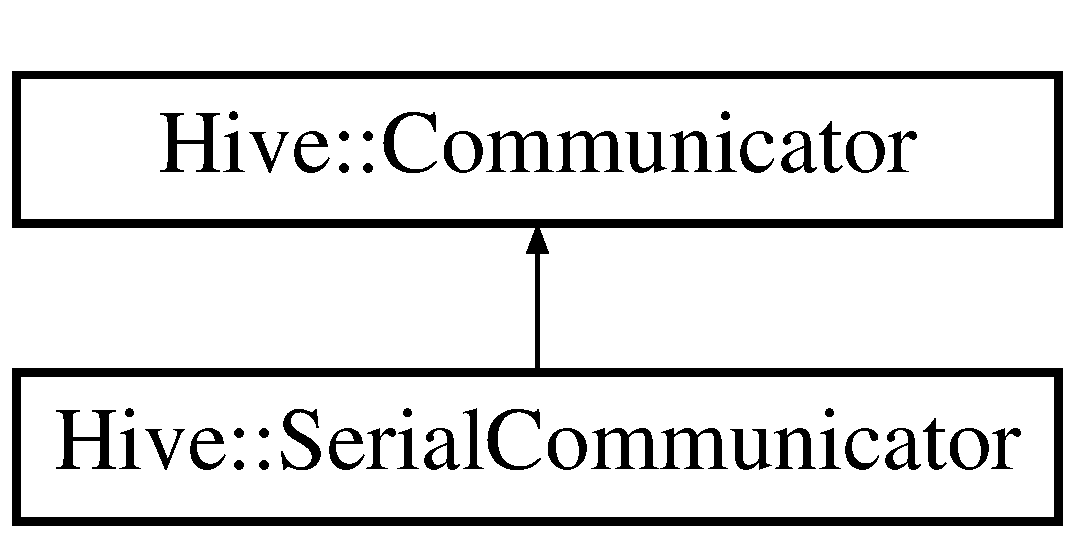
\includegraphics[height=2cm]{classHive_1_1Communicator}
\end{center}
\end{figure}
\subsection*{Public Member Functions}
\begin{CompactItemize}
\item 
{\bf Communicator} ()
\begin{CompactList}\small\item\em constructor \item\end{CompactList}\item 
virtual {\bf $\sim$Communicator} ()
\begin{CompactList}\small\item\em destructor \item\end{CompactList}\item 
virtual void {\bf receiveMessages} ()=0
\begin{CompactList}\small\item\em method for receiving messages \item\end{CompactList}\item 
virtual void {\bf sendMessage} ({\bf Message} m, int dest)=0
\item 
virtual void {\bf propogateAgent} (int agentId, double time)=0
\end{CompactItemize}


\subsection{Constructor \& Destructor Documentation}
\index{Hive::Communicator@{Hive::Communicator}!Communicator@{Communicator}}
\index{Communicator@{Communicator}!Hive::Communicator@{Hive::Communicator}}
\subsubsection[Communicator]{\setlength{\rightskip}{0pt plus 5cm}Hive::Communicator::Communicator ()\hspace{0.3cm}{\tt  [inline]}}\label{classHive_1_1Communicator_34c54aee2bf45015c7146ead7d85615a}


constructor 

\index{Hive::Communicator@{Hive::Communicator}!$\sim$Communicator@{$\sim$Communicator}}
\index{$\sim$Communicator@{$\sim$Communicator}!Hive::Communicator@{Hive::Communicator}}
\subsubsection[$\sim$Communicator]{\setlength{\rightskip}{0pt plus 5cm}virtual Hive::Communicator::$\sim$Communicator ()\hspace{0.3cm}{\tt  [inline, virtual]}}\label{classHive_1_1Communicator_e0395137accdfcbc7cc85e6999eaffe4}


destructor 



\subsection{Member Function Documentation}
\index{Hive::Communicator@{Hive::Communicator}!receiveMessages@{receiveMessages}}
\index{receiveMessages@{receiveMessages}!Hive::Communicator@{Hive::Communicator}}
\subsubsection[receiveMessages]{\setlength{\rightskip}{0pt plus 5cm}virtual void Hive::Communicator::receiveMessages ()\hspace{0.3cm}{\tt  [pure virtual]}}\label{classHive_1_1Communicator_987b52b99ca4639a198f45c0c74db179}


method for receiving messages 



Implemented in {\bf Hive::SerialCommunicator} \doxyref{}{p.}{classHive_1_1SerialCommunicator_020ed57d330b13e4919357dedc72d2f0}.\index{Hive::Communicator@{Hive::Communicator}!sendMessage@{sendMessage}}
\index{sendMessage@{sendMessage}!Hive::Communicator@{Hive::Communicator}}
\subsubsection[sendMessage]{\setlength{\rightskip}{0pt plus 5cm}virtual void Hive::Communicator::sendMessage ({\bf Message} {\em m}, \/  int {\em dest})\hspace{0.3cm}{\tt  [pure virtual]}}\label{classHive_1_1Communicator_7781e9b8494ed71c91769640bef5e6a3}


method for sending messages \begin{Desc}
\item[Parameters:]
\begin{description}
\item[{\em m}]message to be send \item[{\em dest}]identifyer of destination \end{description}
\end{Desc}


Implemented in {\bf Hive::SerialCommunicator} \doxyref{}{p.}{classHive_1_1SerialCommunicator_3a50ba8f646e6b63d44707d7bf9e345b}.

Referenced by Hive::Agent::propagate().\index{Hive::Communicator@{Hive::Communicator}!propogateAgent@{propogateAgent}}
\index{propogateAgent@{propogateAgent}!Hive::Communicator@{Hive::Communicator}}
\subsubsection[propogateAgent]{\setlength{\rightskip}{0pt plus 5cm}virtual void Hive::Communicator::propogateAgent (int {\em agentId}, \/  double {\em time})\hspace{0.3cm}{\tt  [pure virtual]}}\label{classHive_1_1Communicator_8d803da79f8f88bf75a9a306e7676f73}




Implemented in {\bf Hive::SerialCommunicator} \doxyref{}{p.}{classHive_1_1SerialCommunicator_54021e56fa2936e82c0e9e3d6287cf28}.

Referenced by Hive::Agent::propagate().

The documentation for this class was generated from the following file:\begin{CompactItemize}
\item 
{\bf communicator.hh}\end{CompactItemize}

\section{Hive::Composer Class Reference}
\label{classHive_1_1Composer}\index{Hive::Composer@{Hive::Composer}}
{\tt \#include $<$composer.hh$>$}

Inheritance diagram for Hive::Composer::\begin{figure}[H]
\begin{center}
\leavevmode
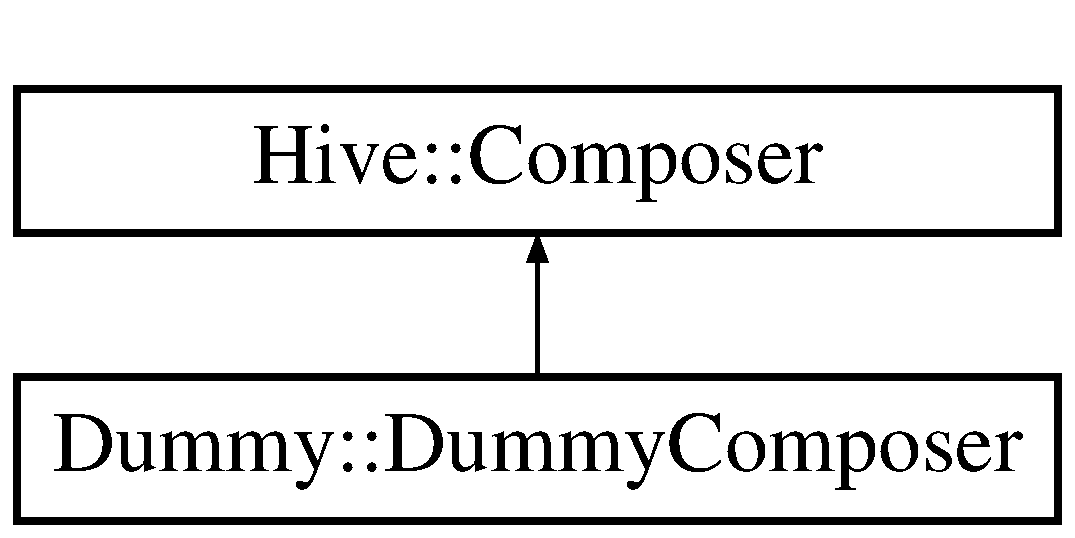
\includegraphics[height=2cm]{classHive_1_1Composer}
\end{center}
\end{figure}


\subsection{Detailed Description}
this class sets up the entire simulation. 

the composer sets up the entire simulation by coordinating all file reading, agent construction and agent initialisation. the setup of a simulation starts with the initialisation of the agentfactories. subsequently the agents are produced and the hierarchy among the agents is established.

\begin{Desc}
\item[{\bf Todo}]Everything\end{Desc}
\begin{Desc}
\item[Author:]Garrit Jentsch\end{Desc}
\begin{Desc}
\item[Date:]13th of Oct, 2009 last edited: 10-14-2009 by Garrit and Michael \end{Desc}
\subsection*{Public Member Functions}
\begin{CompactItemize}
\item 
{\bf Composer} ()
\begin{CompactList}\small\item\em constructor \item\end{CompactList}\item 
virtual {\bf $\sim$Composer} ()
\begin{CompactList}\small\item\em destructor \item\end{CompactList}\item 
{\bf Agent} $\ast$ {\bf getTopLevelAgent} ()
\item 
virtual void {\bf setupSimulation} ()=0
\end{CompactItemize}
\subsection*{Protected Member Functions}
\begin{CompactItemize}
\item 
virtual void {\bf initializeAgentFactories} ()=0
\item 
virtual void {\bf setupAgentHierarchy} ()=0
\item 
virtual {\bf Agent} $\ast$ {\bf createAgent} ({\bf AgentFactory} \&af)=0
\end{CompactItemize}
\subsection*{Protected Attributes}
\begin{CompactItemize}
\item 
{\bf Agent} $\ast$ {\bf maestro}
\begin{CompactList}\small\item\em top level agent \item\end{CompactList}\item 
vector$<$ {\bf Agent} $\ast$ $>$ {\bf orchestra}
\begin{CompactList}\small\item\em vector of agents \item\end{CompactList}\item 
{\bf System} $\ast$ {\bf sys}
\begin{CompactList}\small\item\em system containing the information about the types of agents which can exist in the simulation \item\end{CompactList}\item 
vector$<$ {\bf AgentFactory} $\ast$ $>$ {\bf factories}
\begin{CompactList}\small\item\em vector of agentfactories for agent setup \item\end{CompactList}\end{CompactItemize}


\subsection{Constructor \& Destructor Documentation}
\index{Hive::Composer@{Hive::Composer}!Composer@{Composer}}
\index{Composer@{Composer}!Hive::Composer@{Hive::Composer}}
\subsubsection[Composer]{\setlength{\rightskip}{0pt plus 5cm}Hive::Composer::Composer ()\hspace{0.3cm}{\tt  [inline]}}\label{classHive_1_1Composer_c0b7e7cf4fca7abce2b316812e440a80}


constructor 

\index{Hive::Composer@{Hive::Composer}!$\sim$Composer@{$\sim$Composer}}
\index{$\sim$Composer@{$\sim$Composer}!Hive::Composer@{Hive::Composer}}
\subsubsection[$\sim$Composer]{\setlength{\rightskip}{0pt plus 5cm}virtual Hive::Composer::$\sim$Composer ()\hspace{0.3cm}{\tt  [inline, virtual]}}\label{classHive_1_1Composer_06bcede77609a1e973b59f2183769b18}


destructor 



\subsection{Member Function Documentation}
\index{Hive::Composer@{Hive::Composer}!getTopLevelAgent@{getTopLevelAgent}}
\index{getTopLevelAgent@{getTopLevelAgent}!Hive::Composer@{Hive::Composer}}
\subsubsection[getTopLevelAgent]{\setlength{\rightskip}{0pt plus 5cm}{\bf Agent}$\ast$ Hive::Composer::getTopLevelAgent ()\hspace{0.3cm}{\tt  [inline]}}\label{classHive_1_1Composer_92ed69614640227031451c47c70729a6}


returns pointer to the top level agent \begin{Desc}
\item[Returns:]maestro \end{Desc}


Reimplemented in {\bf Dummy::DummyComposer} \doxyref{}{p.}{classDummy_1_1DummyComposer_cc2ae43b60524d23de72bd9905beaeac}.

References maestro.

Referenced by main().\index{Hive::Composer@{Hive::Composer}!setupSimulation@{setupSimulation}}
\index{setupSimulation@{setupSimulation}!Hive::Composer@{Hive::Composer}}
\subsubsection[setupSimulation]{\setlength{\rightskip}{0pt plus 5cm}virtual void Hive::Composer::setupSimulation ()\hspace{0.3cm}{\tt  [pure virtual]}}\label{classHive_1_1Composer_78092e6e6298ee36ca99ad2aa4daf14e}


top level method for constructing the simulation. for the beginning we will re-implement this method for each new simulation 

Implemented in {\bf Dummy::DummyComposer} \doxyref{}{p.}{classDummy_1_1DummyComposer_c41abf23b1b256ea7a1bdc90d41ab0c7}.

Referenced by main().\index{Hive::Composer@{Hive::Composer}!initializeAgentFactories@{initializeAgentFactories}}
\index{initializeAgentFactories@{initializeAgentFactories}!Hive::Composer@{Hive::Composer}}
\subsubsection[initializeAgentFactories]{\setlength{\rightskip}{0pt plus 5cm}virtual void Hive::Composer::initializeAgentFactories ()\hspace{0.3cm}{\tt  [protected, pure virtual]}}\label{classHive_1_1Composer_3e01c2d9e3317b13bb56954e8b574a5f}


prepare agent factories for agent setup 

Implemented in {\bf Dummy::DummyComposer} \doxyref{}{p.}{classDummy_1_1DummyComposer_cb07bc11db1d12676a8552a60af7a89a}.\index{Hive::Composer@{Hive::Composer}!setupAgentHierarchy@{setupAgentHierarchy}}
\index{setupAgentHierarchy@{setupAgentHierarchy}!Hive::Composer@{Hive::Composer}}
\subsubsection[setupAgentHierarchy]{\setlength{\rightskip}{0pt plus 5cm}virtual void Hive::Composer::setupAgentHierarchy ()\hspace{0.3cm}{\tt  [protected, pure virtual]}}\label{classHive_1_1Composer_6e79138677a66e554b61b52132bb2e1c}


establishes child parent relationships among agents 

Implemented in {\bf Dummy::DummyComposer} \doxyref{}{p.}{classDummy_1_1DummyComposer_ed2fc12d5c5141cb3df0f496772123f8}.\index{Hive::Composer@{Hive::Composer}!createAgent@{createAgent}}
\index{createAgent@{createAgent}!Hive::Composer@{Hive::Composer}}
\subsubsection[createAgent]{\setlength{\rightskip}{0pt plus 5cm}virtual {\bf Agent}$\ast$ Hive::Composer::createAgent ({\bf AgentFactory} \& {\em af})\hspace{0.3cm}{\tt  [protected, pure virtual]}}\label{classHive_1_1Composer_cb6ac88b92f7c7c4b5f618fd3fb13e27}


creates an agent \begin{Desc}
\item[Parameters:]
\begin{description}
\item[{\em af}]agentfactory that does the actual creation of agents. \end{description}
\end{Desc}
\begin{Desc}
\item[Returns:]pointer to created agent \end{Desc}


Implemented in {\bf Dummy::DummyComposer} \doxyref{}{p.}{classDummy_1_1DummyComposer_6c2c70c853ab18940fc8afb7cc6f5521}.

\subsection{Member Data Documentation}
\index{Hive::Composer@{Hive::Composer}!maestro@{maestro}}
\index{maestro@{maestro}!Hive::Composer@{Hive::Composer}}
\subsubsection[maestro]{\setlength{\rightskip}{0pt plus 5cm}{\bf Agent}$\ast$ {\bf Hive::Composer::maestro}\hspace{0.3cm}{\tt  [protected]}}\label{classHive_1_1Composer_0542c667ce11ee5d525987b8e2c2d1d2}


top level agent 



Referenced by Dummy::DummyComposer::getTopLevelAgent(), getTopLevelAgent(), and Dummy::DummyComposer::setupSimulation().\index{Hive::Composer@{Hive::Composer}!orchestra@{orchestra}}
\index{orchestra@{orchestra}!Hive::Composer@{Hive::Composer}}
\subsubsection[orchestra]{\setlength{\rightskip}{0pt plus 5cm}vector$<${\bf Agent}$\ast$ $>$ {\bf Hive::Composer::orchestra}\hspace{0.3cm}{\tt  [protected]}}\label{classHive_1_1Composer_c3024001b742adcbfe14a490b8b982e5}


vector of agents 



Referenced by Dummy::DummyComposer::setupAgentHierarchy(), and Dummy::DummyComposer::setupSimulation().\index{Hive::Composer@{Hive::Composer}!sys@{sys}}
\index{sys@{sys}!Hive::Composer@{Hive::Composer}}
\subsubsection[sys]{\setlength{\rightskip}{0pt plus 5cm}{\bf System}$\ast$ {\bf Hive::Composer::sys}\hspace{0.3cm}{\tt  [protected]}}\label{classHive_1_1Composer_28633951b1fe7e0d3b0f92bf68c60337}


system containing the information about the types of agents which can exist in the simulation 

\index{Hive::Composer@{Hive::Composer}!factories@{factories}}
\index{factories@{factories}!Hive::Composer@{Hive::Composer}}
\subsubsection[factories]{\setlength{\rightskip}{0pt plus 5cm}vector$<${\bf AgentFactory}$\ast$ $>$ {\bf Hive::Composer::factories}\hspace{0.3cm}{\tt  [protected]}}\label{classHive_1_1Composer_6fa6225ae6127e142f38b10aea132679}


vector of agentfactories for agent setup 



Referenced by Dummy::DummyComposer::initializeAgentFactories(), and Dummy::DummyComposer::setupSimulation().

The documentation for this class was generated from the following file:\begin{CompactItemize}
\item 
{\bf composer.hh}\end{CompactItemize}

\section{Hive::Data Class Reference}
\label{classHive_1_1Data}\index{Hive::Data@{Hive::Data}}
{\tt \#include $<$data.hh$>$}

Inheritance diagram for Hive::Data::\begin{figure}[H]
\begin{center}
\leavevmode
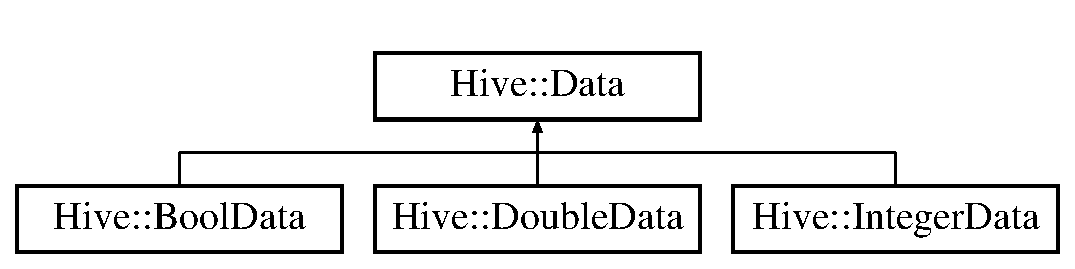
\includegraphics[height=2cm]{classHive_1_1Data}
\end{center}
\end{figure}


\subsection{Detailed Description}
individual element of the database 

abstract class data. all data items stored in the database will have to comply with this interface.

\begin{Desc}
\item[{\bf Todo}]\end{Desc}
\begin{Desc}
\item[Date:]Oct 7, 2009 Last edited: Oct 14, 2009 by Garrit and Michael\end{Desc}
\begin{Desc}
\item[Author:]Garrit Jentsch \end{Desc}
\subsection*{Public Member Functions}
\begin{CompactItemize}
\item 
{\bf Data} (string type)
\item 
virtual {\bf $\sim$Data} ()
\begin{CompactList}\small\item\em Destructor. \item\end{CompactList}\item 
virtual void {\bf printContent} (ostream \&out)=0
\begin{CompactList}\small\item\em virtual method for print the content of a data item on sterr. \item\end{CompactList}\item 
string {\bf getType} () const 
\end{CompactItemize}
\subsection*{Protected Attributes}
\begin{CompactItemize}
\item 
string {\bf datatype}
\begin{CompactList}\small\item\em name of type of data \item\end{CompactList}\end{CompactItemize}


\subsection{Constructor \& Destructor Documentation}
\index{Hive::Data@{Hive::Data}!Data@{Data}}
\index{Data@{Data}!Hive::Data@{Hive::Data}}
\subsubsection[Data]{\setlength{\rightskip}{0pt plus 5cm}Hive::Data::Data (string {\em type})\hspace{0.3cm}{\tt  [inline]}}\label{classHive_1_1Data_6cea772bb6505ce3cb43a210ad7833e7}


constructor \begin{Desc}
\item[Parameters:]
\begin{description}
\item[{\em s}]typename \end{description}
\end{Desc}


References datatype.\index{Hive::Data@{Hive::Data}!$\sim$Data@{$\sim$Data}}
\index{$\sim$Data@{$\sim$Data}!Hive::Data@{Hive::Data}}
\subsubsection[$\sim$Data]{\setlength{\rightskip}{0pt plus 5cm}virtual Hive::Data::$\sim$Data ()\hspace{0.3cm}{\tt  [inline, virtual]}}\label{classHive_1_1Data_5c1113a060d8e715409f042b8d261742}


Destructor. 



\subsection{Member Function Documentation}
\index{Hive::Data@{Hive::Data}!printContent@{printContent}}
\index{printContent@{printContent}!Hive::Data@{Hive::Data}}
\subsubsection[printContent]{\setlength{\rightskip}{0pt plus 5cm}virtual void Hive::Data::printContent (ostream \& {\em out})\hspace{0.3cm}{\tt  [pure virtual]}}\label{classHive_1_1Data_a168edcfa6efd38fe88d72c5162fd8d1}


virtual method for print the content of a data item on sterr. 



Implemented in {\bf Hive::IntegerData} \doxyref{}{p.}{classHive_1_1IntegerData_c8b7d3312b0335c50a0e74aa8bf6a2c0}, {\bf Hive::DoubleData} \doxyref{}{p.}{classHive_1_1DoubleData_96e0192b6ee96ac57fde048f7e854432}, and {\bf Hive::BoolData} \doxyref{}{p.}{classHive_1_1BoolData_4480d929f6baf36ac991c346e4a4b3ea}.\index{Hive::Data@{Hive::Data}!getType@{getType}}
\index{getType@{getType}!Hive::Data@{Hive::Data}}
\subsubsection[getType]{\setlength{\rightskip}{0pt plus 5cm}string Hive::Data::getType () const\hspace{0.3cm}{\tt  [inline]}}\label{classHive_1_1Data_3c2bfec7dc73db3139f75923417517c5}


returns type name of data \begin{Desc}
\item[Returns:]typename \end{Desc}


References datatype.

Referenced by Dummy::DummyWaveAction::fire().

\subsection{Member Data Documentation}
\index{Hive::Data@{Hive::Data}!datatype@{datatype}}
\index{datatype@{datatype}!Hive::Data@{Hive::Data}}
\subsubsection[datatype]{\setlength{\rightskip}{0pt plus 5cm}string {\bf Hive::Data::datatype}\hspace{0.3cm}{\tt  [protected]}}\label{classHive_1_1Data_26773fc7de37e57ea0b216d766027204}


name of type of data 



Referenced by Data(), getType(), Hive::BoolData::printContent(), Hive::DoubleData::printContent(), and Hive::IntegerData::printContent().

The documentation for this class was generated from the following file:\begin{CompactItemize}
\item 
{\bf data.hh}\end{CompactItemize}

\section{Hive::Database Class Reference}
\label{classHive_1_1Database}\index{Hive::Database@{Hive::Database}}
{\tt \#include $<$database.hh$>$}



\subsection{Detailed Description}
\doxyref{Database}{p.}{classHive_1_1Database} of an agent. 

The database of the agent class stores all of the agent's data. This is the most radical way for a generic database in that a database is a vector of void pointers.

\begin{Desc}
\item[{\bf Todo}]Implementation\end{Desc}
\begin{Desc}
\item[Date:]Started: Oct 7th, 2009 Last edited: Oct 14th, 2009 by Garrit and Michael \end{Desc}
\subsection*{Public Member Functions}
\begin{CompactItemize}
\item 
{\bf Database} ()
\begin{CompactList}\small\item\em Constructor. \item\end{CompactList}\item 
{\bf $\sim$Database} ()
\begin{CompactList}\small\item\em Destructor. \item\end{CompactList}\item 
void {\bf setup} ()
\item 
void {\bf dumpDataBase} ({\bf OutputWriter} $\ast$ow)
\item 
void {\bf addData} (string name, {\bf Data} $\ast$data)
\item 
void {\bf eraseDataItem} (string name)
\item 
{\bf Data} $\ast$ {\bf getDataItem} (string name)
\item 
void {\bf readDataBase} ({\bf InputDataReader} $\ast$ir)
\item 
void {\bf returnPointerToData} (string name, {\bf Data} $\ast$\&ptr)
\item 
bool {\bf existsDataItem} (string name)
\end{CompactItemize}
\subsection*{Protected Attributes}
\begin{CompactItemize}
\item 
vector$<$ {\bf Data} $\ast$ $>$ {\bf real\_\-database}
\begin{CompactList}\small\item\em the database is really nothing else but a vector of pointers to data objects \item\end{CompactList}\item 
map$<$ string, int $>$ {\bf data\_\-position\_\-identifyer}
\begin{CompactList}\small\item\em map to give a name to the data items stored in the database \item\end{CompactList}\end{CompactItemize}


\subsection{Constructor \& Destructor Documentation}
\index{Hive::Database@{Hive::Database}!Database@{Database}}
\index{Database@{Database}!Hive::Database@{Hive::Database}}
\subsubsection[Database]{\setlength{\rightskip}{0pt plus 5cm}Database::Database ()}\label{classHive_1_1Database_4703c80e6969d33565ea340f768fdadf}


Constructor. 

\index{Hive::Database@{Hive::Database}!$\sim$Database@{$\sim$Database}}
\index{$\sim$Database@{$\sim$Database}!Hive::Database@{Hive::Database}}
\subsubsection[$\sim$Database]{\setlength{\rightskip}{0pt plus 5cm}Database::$\sim$Database ()}\label{classHive_1_1Database_84d399a2ad58d69daab9b05330e1316d}


Destructor. 



\subsection{Member Function Documentation}
\index{Hive::Database@{Hive::Database}!setup@{setup}}
\index{setup@{setup}!Hive::Database@{Hive::Database}}
\subsubsection[setup]{\setlength{\rightskip}{0pt plus 5cm}void Database::setup ()}\label{classHive_1_1Database_8aa21b2c14a496033b90030dbef746b7}


outputs the entire database \begin{Desc}
\item[Parameters:]
\begin{description}
\item[{\em ow}]Pointer to the \doxyref{OutputWriter}{p.}{classHive_1_1OutputWriter} that outputs the database \end{description}
\end{Desc}
\index{Hive::Database@{Hive::Database}!dumpDataBase@{dumpDataBase}}
\index{dumpDataBase@{dumpDataBase}!Hive::Database@{Hive::Database}}
\subsubsection[dumpDataBase]{\setlength{\rightskip}{0pt plus 5cm}void Database::dumpDataBase ({\bf OutputWriter} $\ast$ {\em ow})}\label{classHive_1_1Database_b5a71b1729cdda881c9240f7cc1c2b98}


outputs the entire database \begin{Desc}
\item[Parameters:]
\begin{description}
\item[{\em ow}]Pointer to the \doxyref{OutputWriter}{p.}{classHive_1_1OutputWriter} that outputs the database \end{description}
\end{Desc}


References real\_\-database.\index{Hive::Database@{Hive::Database}!addData@{addData}}
\index{addData@{addData}!Hive::Database@{Hive::Database}}
\subsubsection[addData]{\setlength{\rightskip}{0pt plus 5cm}void Database::addData (string {\em name}, \/  {\bf Data} $\ast$ {\em data})}\label{classHive_1_1Database_203a8eb871aeffd3310bb73d263ff5a9}


adds data to the database \begin{Desc}
\item[Parameters:]
\begin{description}
\item[{\em name}]Name of the variable to be added \item[{\em ptr}]Pointer to the data to be added \end{description}
\end{Desc}


References data\_\-position\_\-identifyer, and real\_\-database.

Referenced by Dummy::DummyAgentFactory::createAgent(), and Hive::DummySimulator::DummySimulator().\index{Hive::Database@{Hive::Database}!eraseDataItem@{eraseDataItem}}
\index{eraseDataItem@{eraseDataItem}!Hive::Database@{Hive::Database}}
\subsubsection[eraseDataItem]{\setlength{\rightskip}{0pt plus 5cm}void Database::eraseDataItem (string {\em name})}\label{classHive_1_1Database_da3c540517d0d858d925c92efbca1ee6}


removes data item form the database \begin{Desc}
\item[Parameters:]
\begin{description}
\item[{\em name}]Name of data item to be removed. \end{description}
\end{Desc}
\index{Hive::Database@{Hive::Database}!getDataItem@{getDataItem}}
\index{getDataItem@{getDataItem}!Hive::Database@{Hive::Database}}
\subsubsection[getDataItem]{\setlength{\rightskip}{0pt plus 5cm}{\bf Data} $\ast$ Database::getDataItem (string {\em name})}\label{classHive_1_1Database_f5b70a3d1c09f91e8116a299ead84874}


returns a data item \begin{Desc}
\item[Parameters:]
\begin{description}
\item[{\em name}]identifyer of data item \end{description}
\end{Desc}
\begin{Desc}
\item[Returns:]pointer to data item \end{Desc}


References data\_\-position\_\-identifyer, and real\_\-database.

Referenced by Dummy::DummyWaveAction::fire(), Hive::DummySimulator::step(), and Hive::DummySimulator::synchroniseWithDatabase().\index{Hive::Database@{Hive::Database}!readDataBase@{readDataBase}}
\index{readDataBase@{readDataBase}!Hive::Database@{Hive::Database}}
\subsubsection[readDataBase]{\setlength{\rightskip}{0pt plus 5cm}void Database::readDataBase ({\bf InputDataReader} $\ast$ {\em ir})}\label{classHive_1_1Database_820a6511feee01ab831deabc187c2262}


set up a database by using an input reader \begin{Desc}
\item[Parameters:]
\begin{description}
\item[{\em ir}]Pointer to an InputReader \end{description}
\end{Desc}
\index{Hive::Database@{Hive::Database}!returnPointerToData@{returnPointerToData}}
\index{returnPointerToData@{returnPointerToData}!Hive::Database@{Hive::Database}}
\subsubsection[returnPointerToData]{\setlength{\rightskip}{0pt plus 5cm}void Database::returnPointerToData (string {\em name}, \/  {\bf Data} $\ast$\& {\em ptr})}\label{classHive_1_1Database_46896d00038c00ca0ed8671656a27344}


returns pointer to data item \begin{Desc}
\item[Parameters:]
\begin{description}
\item[{\em name}]Name of variable that one wishes to obtain a pointer to. \item[{\em ptr}]Pointer to the desired variable. \end{description}
\end{Desc}


References data\_\-position\_\-identifyer, and real\_\-database.\index{Hive::Database@{Hive::Database}!existsDataItem@{existsDataItem}}
\index{existsDataItem@{existsDataItem}!Hive::Database@{Hive::Database}}
\subsubsection[existsDataItem]{\setlength{\rightskip}{0pt plus 5cm}bool Database::existsDataItem (string {\em name})}\label{classHive_1_1Database_b8e62e5705be8b286775576271b5e1f2}


ask for existence of a data\_\-item \begin{Desc}
\item[Parameters:]
\begin{description}
\item[{\em name}]name of dataitem \end{description}
\end{Desc}
\begin{Desc}
\item[Returns:]existence \end{Desc}


References data\_\-position\_\-identifyer.

\subsection{Member Data Documentation}
\index{Hive::Database@{Hive::Database}!real\_\-database@{real\_\-database}}
\index{real\_\-database@{real\_\-database}!Hive::Database@{Hive::Database}}
\subsubsection[real\_\-database]{\setlength{\rightskip}{0pt plus 5cm}vector$<${\bf Data} $\ast$$>$ {\bf Hive::Database::real\_\-database}\hspace{0.3cm}{\tt  [protected]}}\label{classHive_1_1Database_04552fae2427e74809fab02759be705d}


the database is really nothing else but a vector of pointers to data objects 



Referenced by addData(), dumpDataBase(), getDataItem(), and returnPointerToData().\index{Hive::Database@{Hive::Database}!data\_\-position\_\-identifyer@{data\_\-position\_\-identifyer}}
\index{data\_\-position\_\-identifyer@{data\_\-position\_\-identifyer}!Hive::Database@{Hive::Database}}
\subsubsection[data\_\-position\_\-identifyer]{\setlength{\rightskip}{0pt plus 5cm}map$<$string, int$>$ {\bf Hive::Database::data\_\-position\_\-identifyer}\hspace{0.3cm}{\tt  [protected]}}\label{classHive_1_1Database_8f1b647aa252e120ddaf4c91c760a1bd}


map to give a name to the data items stored in the database 



Referenced by addData(), existsDataItem(), getDataItem(), and returnPointerToData().

The documentation for this class was generated from the following files:\begin{CompactItemize}
\item 
{\bf database.hh}\item 
{\bf database.cpp}\end{CompactItemize}

\section{Hive::DoubleData Class Reference}
\label{classHive_1_1DoubleData}\index{Hive::DoubleData@{Hive::DoubleData}}
{\tt \#include $<$primitiveData.hh$>$}

Inheritance diagram for Hive::DoubleData::\begin{figure}[H]
\begin{center}
\leavevmode
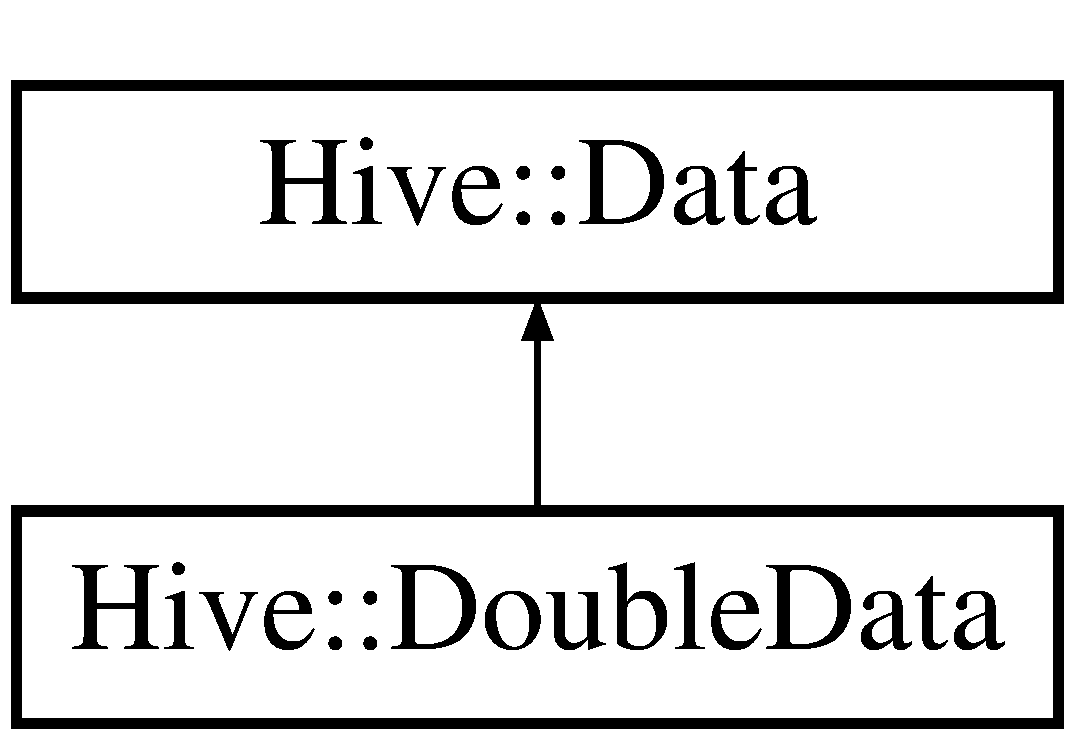
\includegraphics[height=2cm]{classHive_1_1DoubleData}
\end{center}
\end{figure}


\subsection{Detailed Description}
A data object to store double values. 

\begin{Desc}
\item[Date:]Oct 14, 2009 Last edited: Oct 14, 2009 by Garrit and Michael \end{Desc}
\begin{Desc}
\item[Author:]Garrit Jentsch \end{Desc}
\subsection*{Public Member Functions}
\begin{CompactItemize}
\item 
{\bf DoubleData} (string dataName, double value)
\begin{CompactList}\small\item\em default-constructor \item\end{CompactList}\item 
virtual {\bf $\sim$DoubleData} ()
\item 
void {\bf printContent} (ostream \&out)
\begin{CompactList}\small\item\em virtual method for print the content of a data item on sterr. \item\end{CompactList}\item 
string {\bf getDataName} () const 
\item 
double {\bf getDouble} () const 
\item 
void {\bf setDouble} (double newValue)
\end{CompactItemize}


\subsection{Constructor \& Destructor Documentation}
\index{Hive::DoubleData@{Hive::DoubleData}!DoubleData@{DoubleData}}
\index{DoubleData@{DoubleData}!Hive::DoubleData@{Hive::DoubleData}}
\subsubsection[DoubleData]{\setlength{\rightskip}{0pt plus 5cm}DoubleData::DoubleData (string {\em dataName}, \/  double {\em value})}\label{classHive_1_1DoubleData_aa84969490e7856fc4ff6187c9e5b19b}


default-constructor 

\index{Hive::DoubleData@{Hive::DoubleData}!$\sim$DoubleData@{$\sim$DoubleData}}
\index{$\sim$DoubleData@{$\sim$DoubleData}!Hive::DoubleData@{Hive::DoubleData}}
\subsubsection[$\sim$DoubleData]{\setlength{\rightskip}{0pt plus 5cm}virtual Hive::DoubleData::$\sim$DoubleData ()\hspace{0.3cm}{\tt  [inline, virtual]}}\label{classHive_1_1DoubleData_f3b135b1ca71f08340bd56931923056c}




\subsection{Member Function Documentation}
\index{Hive::DoubleData@{Hive::DoubleData}!printContent@{printContent}}
\index{printContent@{printContent}!Hive::DoubleData@{Hive::DoubleData}}
\subsubsection[printContent]{\setlength{\rightskip}{0pt plus 5cm}void DoubleData::printContent (ostream \& {\em out})\hspace{0.3cm}{\tt  [virtual]}}\label{classHive_1_1DoubleData_96e0192b6ee96ac57fde048f7e854432}


virtual method for print the content of a data item on sterr. 



Implements {\bf Hive::Data} \doxyref{}{p.}{classHive_1_1Data_a168edcfa6efd38fe88d72c5162fd8d1}.

References Hive::Data::datatype.\index{Hive::DoubleData@{Hive::DoubleData}!getDataName@{getDataName}}
\index{getDataName@{getDataName}!Hive::DoubleData@{Hive::DoubleData}}
\subsubsection[getDataName]{\setlength{\rightskip}{0pt plus 5cm}string Hive::DoubleData::getDataName () const\hspace{0.3cm}{\tt  [inline]}}\label{classHive_1_1DoubleData_9360adfdd19463002eff09ec618ad967}


\index{Hive::DoubleData@{Hive::DoubleData}!getDouble@{getDouble}}
\index{getDouble@{getDouble}!Hive::DoubleData@{Hive::DoubleData}}
\subsubsection[getDouble]{\setlength{\rightskip}{0pt plus 5cm}double Hive::DoubleData::getDouble () const\hspace{0.3cm}{\tt  [inline]}}\label{classHive_1_1DoubleData_a40c251af1b20a46cfc67eeafd5c1b2f}




Referenced by Hive::DummySimulator::synchroniseWithDatabase().\index{Hive::DoubleData@{Hive::DoubleData}!setDouble@{setDouble}}
\index{setDouble@{setDouble}!Hive::DoubleData@{Hive::DoubleData}}
\subsubsection[setDouble]{\setlength{\rightskip}{0pt plus 5cm}void Hive::DoubleData::setDouble (double {\em newValue})\hspace{0.3cm}{\tt  [inline]}}\label{classHive_1_1DoubleData_85addb821caf045b2dca4d1f8930a234}




Referenced by Hive::DummySimulator::step().

The documentation for this class was generated from the following files:\begin{CompactItemize}
\item 
{\bf primitiveData.hh}\item 
{\bf primitiveData.cpp}\end{CompactItemize}

\section{Dummy::DummyAgentFactory Class Reference}
\label{classDummy_1_1DummyAgentFactory}\index{Dummy::DummyAgentFactory@{Dummy::DummyAgentFactory}}
{\tt \#include $<$dummyagentfactory.hh$>$}

Inheritance diagram for Dummy::DummyAgentFactory::\begin{figure}[H]
\begin{center}
\leavevmode
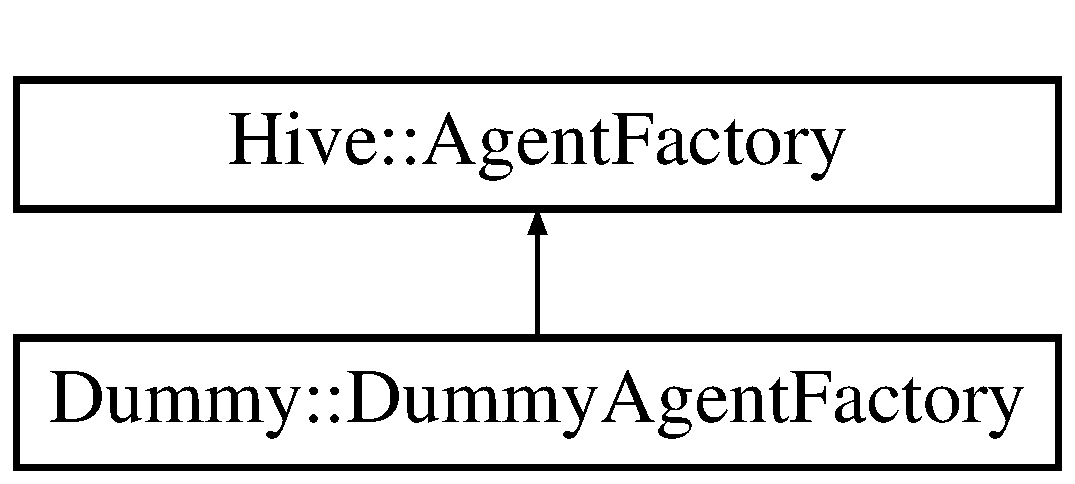
\includegraphics[height=2cm]{classDummy_1_1DummyAgentFactory}
\end{center}
\end{figure}


\subsection{Detailed Description}
simple implementation of an agentfactory 

this is a minimal implemtation of the agentfactory. it generates agents that can not really do anything.

\begin{Desc}
\item[Author:]Garrit Jentsch\end{Desc}
\begin{Desc}
\item[Date:]Oct 14, 2009 last edited Oct 15, 2009 \end{Desc}
\subsection*{Public Member Functions}
\begin{CompactItemize}
\item 
{\bf DummyAgentFactory} ()
\item 
{\bf DummyAgentFactory} ({\bf InputSystemReader} $\ast${\bf isr})
\item 
{\bf Agent} $\ast$ {\bf createAgent} ()
\item 
{\bf Agent} $\ast$ {\bf createAgent} ({\bf Action} $\ast$$\ast$ac)
\item 
{\bf Agent} $\ast$ {\bf duplicateAgent} ({\bf Agent} $\ast$ag)
\end{CompactItemize}
\subsection*{Protected Member Functions}
\begin{CompactItemize}
\item 
void {\bf addActionToAgentsActionSet} ({\bf Action} $\ast$a)
\item 
void {\bf addSimulatorToAgent} ({\bf Simulator} $\ast$s)
\end{CompactItemize}


\subsection{Constructor \& Destructor Documentation}
\index{Dummy::DummyAgentFactory@{Dummy::DummyAgentFactory}!DummyAgentFactory@{DummyAgentFactory}}
\index{DummyAgentFactory@{DummyAgentFactory}!Dummy::DummyAgentFactory@{Dummy::DummyAgentFactory}}
\subsubsection[DummyAgentFactory]{\setlength{\rightskip}{0pt plus 5cm}DummyAgentFactory::DummyAgentFactory ()}\label{classDummy_1_1DummyAgentFactory_2766d99aae0baea748b68019507c2590}


\index{Dummy::DummyAgentFactory@{Dummy::DummyAgentFactory}!DummyAgentFactory@{DummyAgentFactory}}
\index{DummyAgentFactory@{DummyAgentFactory}!Dummy::DummyAgentFactory@{Dummy::DummyAgentFactory}}
\subsubsection[DummyAgentFactory]{\setlength{\rightskip}{0pt plus 5cm}DummyAgentFactory::DummyAgentFactory ({\bf InputSystemReader} $\ast$ {\em isr})}\label{classDummy_1_1DummyAgentFactory_733f884c3a2beaac5991d98dd9e40d34}




\subsection{Member Function Documentation}
\index{Dummy::DummyAgentFactory@{Dummy::DummyAgentFactory}!createAgent@{createAgent}}
\index{createAgent@{createAgent}!Dummy::DummyAgentFactory@{Dummy::DummyAgentFactory}}
\subsubsection[createAgent]{\setlength{\rightskip}{0pt plus 5cm}{\bf Agent} $\ast$ DummyAgentFactory::createAgent ()\hspace{0.3cm}{\tt  [virtual]}}\label{classDummy_1_1DummyAgentFactory_0aec7238d1758a98d59817f49ae1c2c0}


create agent of a certain type. encapsulates everything that has to be done, i.e. it adds actions, simulator, messagegenerators, and communicator to the agent. the simulator is also told to connect to the database and initialize itself. \begin{Desc}
\item[Returns:]pointer to constructed agent \end{Desc}


Implements {\bf Hive::AgentFactory} \doxyref{}{p.}{classHive_1_1AgentFactory_a1e148a842b3f0e2dd11de0ef61bf877}.

References Hive::Agent::addAction(), Hive::Database::addData(), Hive::Agent::addMessageGenerator(), Hive::Agent::addSimulator(), Hive::Agent::getDatabase(), Hive::IntegerData::getDataName(), and Hive::Action::setAgent().\index{Dummy::DummyAgentFactory@{Dummy::DummyAgentFactory}!createAgent@{createAgent}}
\index{createAgent@{createAgent}!Dummy::DummyAgentFactory@{Dummy::DummyAgentFactory}}
\subsubsection[createAgent]{\setlength{\rightskip}{0pt plus 5cm}{\bf Agent} $\ast$ DummyAgentFactory::createAgent ({\bf Action} $\ast$$\ast$ {\em as})\hspace{0.3cm}{\tt  [virtual]}}\label{classDummy_1_1DummyAgentFactory_939e7c2ccee8945187801e6cd92da0df}


create an agent and provide actionset as an argument \begin{Desc}
\item[Parameters:]
\begin{description}
\item[{\em as}]pointer to actionset \end{description}
\end{Desc}


Implements {\bf Hive::AgentFactory} \doxyref{}{p.}{classHive_1_1AgentFactory_40e828a8b7c397c11a3c0ed24e22932d}.\index{Dummy::DummyAgentFactory@{Dummy::DummyAgentFactory}!duplicateAgent@{duplicateAgent}}
\index{duplicateAgent@{duplicateAgent}!Dummy::DummyAgentFactory@{Dummy::DummyAgentFactory}}
\subsubsection[duplicateAgent]{\setlength{\rightskip}{0pt plus 5cm}{\bf Agent} $\ast$ DummyAgentFactory::duplicateAgent ({\bf Agent} $\ast$ {\em ag})\hspace{0.3cm}{\tt  [virtual]}}\label{classDummy_1_1DummyAgentFactory_8ddeb4e5090dac67d921e8a4b89275a7}


copies an agent \begin{Desc}
\item[Parameters:]
\begin{description}
\item[{\em $\ast$ag}]pointer to agent to be copied \end{description}
\end{Desc}
\begin{Desc}
\item[Returns:]pointer to copy \end{Desc}


Implements {\bf Hive::AgentFactory} \doxyref{}{p.}{classHive_1_1AgentFactory_ea99bc08ec4fa2a262244362e7de03f6}.\index{Dummy::DummyAgentFactory@{Dummy::DummyAgentFactory}!addActionToAgentsActionSet@{addActionToAgentsActionSet}}
\index{addActionToAgentsActionSet@{addActionToAgentsActionSet}!Dummy::DummyAgentFactory@{Dummy::DummyAgentFactory}}
\subsubsection[addActionToAgentsActionSet]{\setlength{\rightskip}{0pt plus 5cm}void DummyAgentFactory::addActionToAgentsActionSet ({\bf Action} $\ast$ {\em a})\hspace{0.3cm}{\tt  [protected, virtual]}}\label{classDummy_1_1DummyAgentFactory_f469c5c34c6d26c944d9272c3bff6cb5}


adds an action to the agents action set \begin{Desc}
\item[Parameters:]
\begin{description}
\item[{\em $\ast$a}]pointer to action \end{description}
\end{Desc}


Implements {\bf Hive::AgentFactory} \doxyref{}{p.}{classHive_1_1AgentFactory_978d73e56c472e6ecce59282fa80852e}.\index{Dummy::DummyAgentFactory@{Dummy::DummyAgentFactory}!addSimulatorToAgent@{addSimulatorToAgent}}
\index{addSimulatorToAgent@{addSimulatorToAgent}!Dummy::DummyAgentFactory@{Dummy::DummyAgentFactory}}
\subsubsection[addSimulatorToAgent]{\setlength{\rightskip}{0pt plus 5cm}void DummyAgentFactory::addSimulatorToAgent ({\bf Simulator} $\ast$ {\em s})\hspace{0.3cm}{\tt  [protected, virtual]}}\label{classDummy_1_1DummyAgentFactory_52894893fc20746c63949ee62ff875af}


adds a simulator to the agents simulator set \begin{Desc}
\item[Parameters:]
\begin{description}
\item[{\em $\ast$s}]pointer to simulator \end{description}
\end{Desc}


Implements {\bf Hive::AgentFactory} \doxyref{}{p.}{classHive_1_1AgentFactory_e10d7f9aeb994662565de5fa7d074e87}.

The documentation for this class was generated from the following files:\begin{CompactItemize}
\item 
{\bf dummyagentfactory.hh}\item 
{\bf dummyagentfactory.cpp}\end{CompactItemize}

\section{Dummy::DummyComposer Class Reference}
\label{classDummy_1_1DummyComposer}\index{Dummy::DummyComposer@{Dummy::DummyComposer}}
{\tt \#include $<$dummycomposer.hh$>$}

Inheritance diagram for Dummy::DummyComposer::\begin{figure}[H]
\begin{center}
\leavevmode
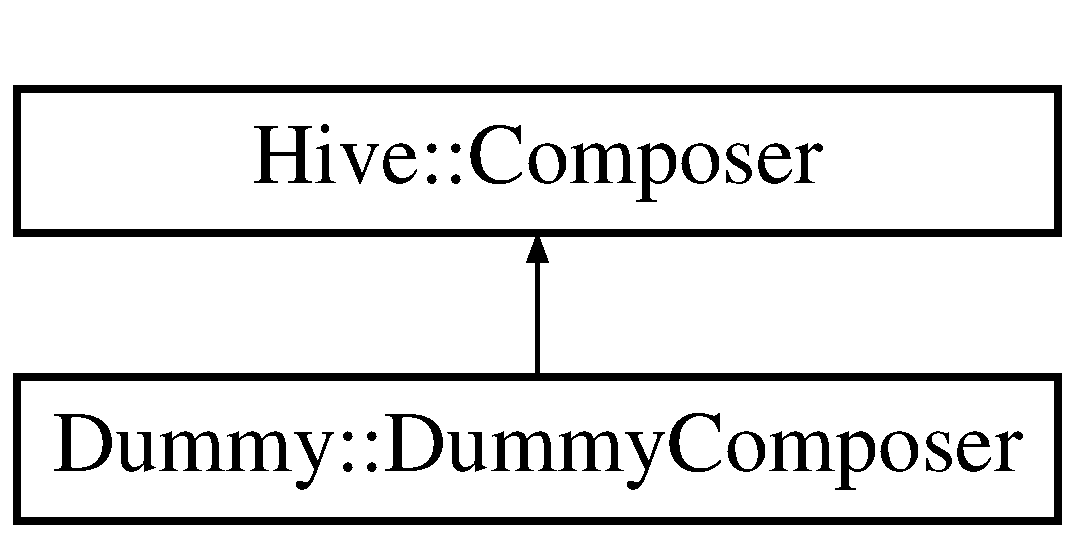
\includegraphics[height=2cm]{classDummy_1_1DummyComposer}
\end{center}
\end{figure}
\subsection*{Public Member Functions}
\begin{CompactItemize}
\item 
{\bf DummyComposer} ()
\item 
{\bf $\sim$DummyComposer} ()
\item 
void {\bf setupSimulation} ()
\end{CompactItemize}
\subsection*{Protected Member Functions}
\begin{CompactItemize}
\item 
void {\bf initializeAgentFactories} ()
\item 
void {\bf setupAgentHierarchy} ()
\item 
{\bf Agent} $\ast$ {\bf getTopLevelAgent} ()
\item 
{\bf Agent} $\ast$ {\bf createAgent} ({\bf AgentFactory} \&)
\end{CompactItemize}


\subsection{Constructor \& Destructor Documentation}
\index{Dummy::DummyComposer@{Dummy::DummyComposer}!DummyComposer@{DummyComposer}}
\index{DummyComposer@{DummyComposer}!Dummy::DummyComposer@{Dummy::DummyComposer}}
\subsubsection[DummyComposer]{\setlength{\rightskip}{0pt plus 5cm}DummyComposer::DummyComposer ()}\label{classDummy_1_1DummyComposer_e6414916b858290875f9af4864d70444}


\index{Dummy::DummyComposer@{Dummy::DummyComposer}!$\sim$DummyComposer@{$\sim$DummyComposer}}
\index{$\sim$DummyComposer@{$\sim$DummyComposer}!Dummy::DummyComposer@{Dummy::DummyComposer}}
\subsubsection[$\sim$DummyComposer]{\setlength{\rightskip}{0pt plus 5cm}DummyComposer::$\sim$DummyComposer ()}\label{classDummy_1_1DummyComposer_897383f39ffa180b8b014bc06af69854}




\subsection{Member Function Documentation}
\index{Dummy::DummyComposer@{Dummy::DummyComposer}!setupSimulation@{setupSimulation}}
\index{setupSimulation@{setupSimulation}!Dummy::DummyComposer@{Dummy::DummyComposer}}
\subsubsection[setupSimulation]{\setlength{\rightskip}{0pt plus 5cm}void DummyComposer::setupSimulation ()\hspace{0.3cm}{\tt  [virtual]}}\label{classDummy_1_1DummyComposer_c41abf23b1b256ea7a1bdc90d41ab0c7}


top level method for constructing the simulation. for the beginning we will re-implement this method for each new simulation 

Implements {\bf Hive::Composer} \doxyref{}{p.}{classHive_1_1Composer_78092e6e6298ee36ca99ad2aa4daf14e}.

References createAgent(), Hive::Composer::factories, initializeAgentFactories(), Hive::Composer::maestro, Hive::Composer::orchestra, and setupAgentHierarchy().\index{Dummy::DummyComposer@{Dummy::DummyComposer}!initializeAgentFactories@{initializeAgentFactories}}
\index{initializeAgentFactories@{initializeAgentFactories}!Dummy::DummyComposer@{Dummy::DummyComposer}}
\subsubsection[initializeAgentFactories]{\setlength{\rightskip}{0pt plus 5cm}void DummyComposer::initializeAgentFactories ()\hspace{0.3cm}{\tt  [protected, virtual]}}\label{classDummy_1_1DummyComposer_cb07bc11db1d12676a8552a60af7a89a}


prepare agent factories for agent setup 

Implements {\bf Hive::Composer} \doxyref{}{p.}{classHive_1_1Composer_3e01c2d9e3317b13bb56954e8b574a5f}.

References Hive::Composer::factories.

Referenced by setupSimulation().\index{Dummy::DummyComposer@{Dummy::DummyComposer}!setupAgentHierarchy@{setupAgentHierarchy}}
\index{setupAgentHierarchy@{setupAgentHierarchy}!Dummy::DummyComposer@{Dummy::DummyComposer}}
\subsubsection[setupAgentHierarchy]{\setlength{\rightskip}{0pt plus 5cm}void DummyComposer::setupAgentHierarchy ()\hspace{0.3cm}{\tt  [protected, virtual]}}\label{classDummy_1_1DummyComposer_ed2fc12d5c5141cb3df0f496772123f8}


establishes child parent relationships among agents 

Implements {\bf Hive::Composer} \doxyref{}{p.}{classHive_1_1Composer_6e79138677a66e554b61b52132bb2e1c}.

References Hive::SerialCommunicator::addAgent(), and Hive::Composer::orchestra.

Referenced by setupSimulation().\index{Dummy::DummyComposer@{Dummy::DummyComposer}!getTopLevelAgent@{getTopLevelAgent}}
\index{getTopLevelAgent@{getTopLevelAgent}!Dummy::DummyComposer@{Dummy::DummyComposer}}
\subsubsection[getTopLevelAgent]{\setlength{\rightskip}{0pt plus 5cm}{\bf Agent} $\ast$ DummyComposer::getTopLevelAgent ()\hspace{0.3cm}{\tt  [protected]}}\label{classDummy_1_1DummyComposer_cc2ae43b60524d23de72bd9905beaeac}


returns pointer to the top level agent \begin{Desc}
\item[Returns:]maestro \end{Desc}


Reimplemented from {\bf Hive::Composer} \doxyref{}{p.}{classHive_1_1Composer_92ed69614640227031451c47c70729a6}.

References Hive::Composer::maestro.\index{Dummy::DummyComposer@{Dummy::DummyComposer}!createAgent@{createAgent}}
\index{createAgent@{createAgent}!Dummy::DummyComposer@{Dummy::DummyComposer}}
\subsubsection[createAgent]{\setlength{\rightskip}{0pt plus 5cm}{\bf Agent} $\ast$ DummyComposer::createAgent ({\bf AgentFactory} \& {\em af})\hspace{0.3cm}{\tt  [protected, virtual]}}\label{classDummy_1_1DummyComposer_6c2c70c853ab18940fc8afb7cc6f5521}


creates an agent \begin{Desc}
\item[Parameters:]
\begin{description}
\item[{\em af}]agentfactory that does the actual creation of agents. \end{description}
\end{Desc}
\begin{Desc}
\item[Returns:]pointer to created agent \end{Desc}


Implements {\bf Hive::Composer} \doxyref{}{p.}{classHive_1_1Composer_cb6ac88b92f7c7c4b5f618fd3fb13e27}.

References Hive::AgentFactory::createAgent().

Referenced by setupSimulation().

The documentation for this class was generated from the following files:\begin{CompactItemize}
\item 
{\bf dummycomposer.hh}\item 
{\bf dummyComposer.cpp}\end{CompactItemize}

\section{Dummy::DummyMessageGenerator Class Reference}
\label{classDummy_1_1DummyMessageGenerator}\index{Dummy::DummyMessageGenerator@{Dummy::DummyMessageGenerator}}
{\tt \#include $<$dummymessagegenerator.hh$>$}

Inheritance diagram for Dummy::DummyMessageGenerator::\begin{figure}[H]
\begin{center}
\leavevmode
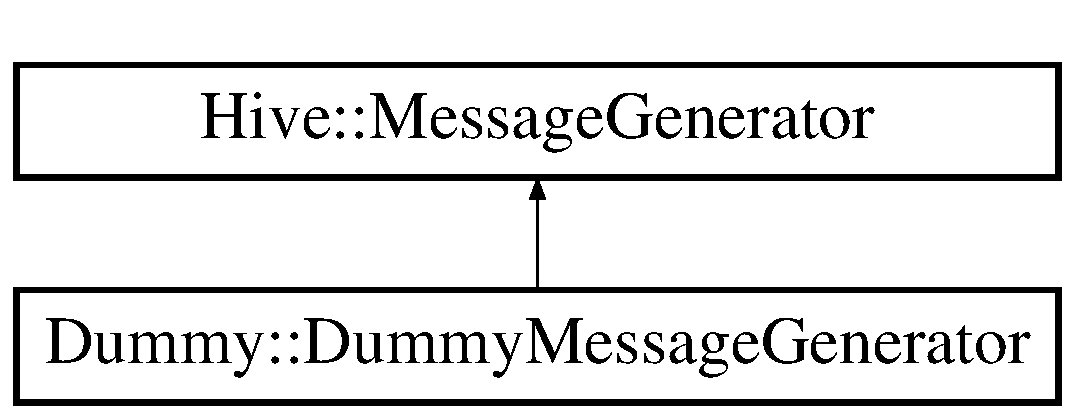
\includegraphics[height=2cm]{classDummy_1_1DummyMessageGenerator}
\end{center}
\end{figure}


\subsection{Detailed Description}
this class implements the messagegenerator 

\begin{Desc}
\item[{\bf Todo}]\end{Desc}
\begin{Desc}
\item[Author:]Garrit Jentsch\end{Desc}
\begin{Desc}
\item[Date:]Oct 15, 2009 last edited 10-15-2009 \end{Desc}
\subsection*{Public Member Functions}
\begin{CompactItemize}
\item 
{\bf DummyMessageGenerator} ()
\item 
{\bf DummyMessageGenerator} ({\bf Agent} $\ast$)
\item 
{\bf $\sim$DummyMessageGenerator} ()
\item 
void {\bf placeMessage} ()
\end{CompactItemize}


\subsection{Constructor \& Destructor Documentation}
\index{Dummy::DummyMessageGenerator@{Dummy::DummyMessageGenerator}!DummyMessageGenerator@{DummyMessageGenerator}}
\index{DummyMessageGenerator@{DummyMessageGenerator}!Dummy::DummyMessageGenerator@{Dummy::DummyMessageGenerator}}
\subsubsection[DummyMessageGenerator]{\setlength{\rightskip}{0pt plus 5cm}DummyMessageGenerator::DummyMessageGenerator ()}\label{classDummy_1_1DummyMessageGenerator_8f7b33594612f29af957b4a364d2a224}


\index{Dummy::DummyMessageGenerator@{Dummy::DummyMessageGenerator}!DummyMessageGenerator@{DummyMessageGenerator}}
\index{DummyMessageGenerator@{DummyMessageGenerator}!Dummy::DummyMessageGenerator@{Dummy::DummyMessageGenerator}}
\subsubsection[DummyMessageGenerator]{\setlength{\rightskip}{0pt plus 5cm}DummyMessageGenerator::DummyMessageGenerator ({\bf Agent} $\ast$ {\em ag})}\label{classDummy_1_1DummyMessageGenerator_7a7c13e499142e79927209c0e29135c7}


\index{Dummy::DummyMessageGenerator@{Dummy::DummyMessageGenerator}!$\sim$DummyMessageGenerator@{$\sim$DummyMessageGenerator}}
\index{$\sim$DummyMessageGenerator@{$\sim$DummyMessageGenerator}!Dummy::DummyMessageGenerator@{Dummy::DummyMessageGenerator}}
\subsubsection[$\sim$DummyMessageGenerator]{\setlength{\rightskip}{0pt plus 5cm}DummyMessageGenerator::$\sim$DummyMessageGenerator ()}\label{classDummy_1_1DummyMessageGenerator_0542d216ef2dc0c0b522e9185c5c20c1}




\subsection{Member Function Documentation}
\index{Dummy::DummyMessageGenerator@{Dummy::DummyMessageGenerator}!placeMessage@{placeMessage}}
\index{placeMessage@{placeMessage}!Dummy::DummyMessageGenerator@{Dummy::DummyMessageGenerator}}
\subsubsection[placeMessage]{\setlength{\rightskip}{0pt plus 5cm}void DummyMessageGenerator::placeMessage ()\hspace{0.3cm}{\tt  [virtual]}}\label{classDummy_1_1DummyMessageGenerator_5a7af3c76d74a53211e440fc86514d0c}


generate message and puts it into the outbox of the source agent 

Implements {\bf Hive::MessageGenerator} \doxyref{}{p.}{classHive_1_1MessageGenerator_874d881a3aeff02ca53391714f659a20}.

References Hive::Agent::placeMessageOnMessageQueue(), Hive::Message::setAction(), Hive::Message::setArgument(), and Hive::MessageGenerator::source.

The documentation for this class was generated from the following files:\begin{CompactItemize}
\item 
{\bf dummymessagegenerator.hh}\item 
{\bf dummymessagegenerator.cpp}\end{CompactItemize}

\section{Hive::DummySimulator Class Reference}
\label{classHive_1_1DummySimulator}\index{Hive::DummySimulator@{Hive::DummySimulator}}
{\tt \#include $<$dummySimulator.hh$>$}

Inheritance diagram for Hive::DummySimulator::\begin{figure}[H]
\begin{center}
\leavevmode
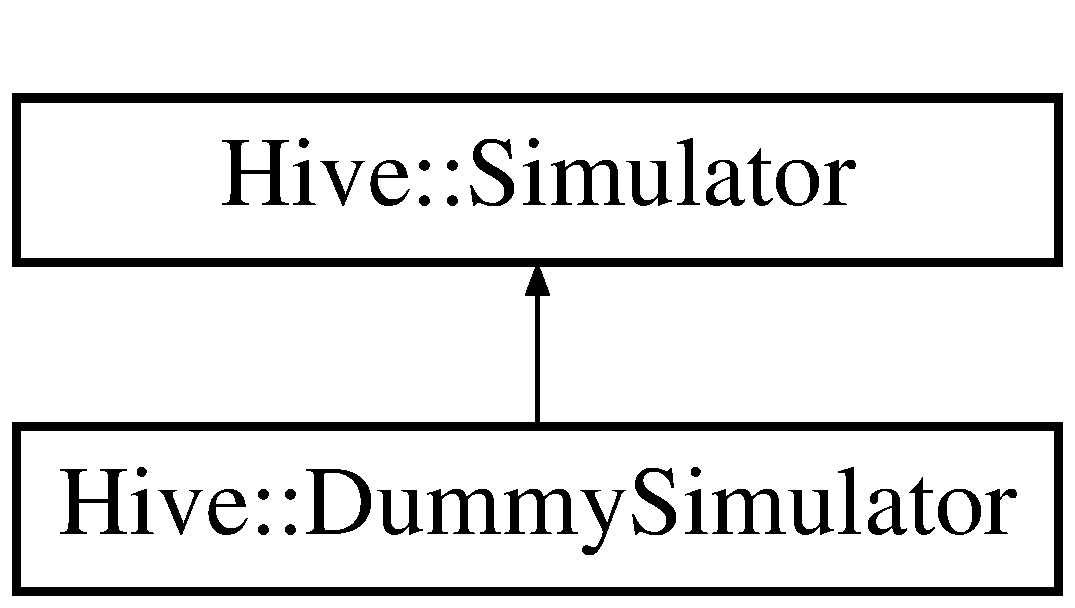
\includegraphics[height=2cm]{classHive_1_1DummySimulator}
\end{center}
\end{figure}
\subsection*{Public Member Functions}
\begin{CompactItemize}
\item 
{\bf DummySimulator} ({\bf Agent} $\ast$a)
\begin{CompactList}\small\item\em Constructor. \item\end{CompactList}\item 
{\bf $\sim$DummySimulator} ()
\begin{CompactList}\small\item\em destructor \item\end{CompactList}\item 
void {\bf step} (double t)
\item 
void {\bf prepare} ()
\item 
void {\bf synchroniseWithDatabase} ()
\end{CompactItemize}
\subsection*{Protected Member Functions}
\begin{CompactItemize}
\item 
void {\bf initialise} ()
\end{CompactItemize}


\subsection{Constructor \& Destructor Documentation}
\index{Hive::DummySimulator@{Hive::DummySimulator}!DummySimulator@{DummySimulator}}
\index{DummySimulator@{DummySimulator}!Hive::DummySimulator@{Hive::DummySimulator}}
\subsubsection[DummySimulator]{\setlength{\rightskip}{0pt plus 5cm}DummySimulator::DummySimulator ({\bf Agent} $\ast$ {\em a})}\label{classHive_1_1DummySimulator_dc2eddec79b77c360ea190782f7ebc3e}


Constructor. 



References Hive::Database::addData(), Hive::Simulator::agent, and Hive::Agent::getDatabase().\index{Hive::DummySimulator@{Hive::DummySimulator}!$\sim$DummySimulator@{$\sim$DummySimulator}}
\index{$\sim$DummySimulator@{$\sim$DummySimulator}!Hive::DummySimulator@{Hive::DummySimulator}}
\subsubsection[$\sim$DummySimulator]{\setlength{\rightskip}{0pt plus 5cm}DummySimulator::$\sim$DummySimulator ()}\label{classHive_1_1DummySimulator_660a64ddb93b9f26c03d1d127af188c5}


destructor 



\subsection{Member Function Documentation}
\index{Hive::DummySimulator@{Hive::DummySimulator}!step@{step}}
\index{step@{step}!Hive::DummySimulator@{Hive::DummySimulator}}
\subsubsection[step]{\setlength{\rightskip}{0pt plus 5cm}void DummySimulator::step (double {\em t})\hspace{0.3cm}{\tt  [virtual]}}\label{classHive_1_1DummySimulator_fa489e06187269a63ed18143272d2ef3}


integrate the system for a timestep \begin{Desc}
\item[Parameters:]
\begin{description}
\item[{\em t}]timestep \end{description}
\end{Desc}


Implements {\bf Hive::Simulator} \doxyref{}{p.}{classHive_1_1Simulator_eec111bc06eafdbf4cbc96389c4819d3}.

References Hive::Database::getDataItem(), Util::RANDOM\_\-CLOSED(), and Hive::DoubleData::setDouble().\index{Hive::DummySimulator@{Hive::DummySimulator}!prepare@{prepare}}
\index{prepare@{prepare}!Hive::DummySimulator@{Hive::DummySimulator}}
\subsubsection[prepare]{\setlength{\rightskip}{0pt plus 5cm}void DummySimulator::prepare ()\hspace{0.3cm}{\tt  [virtual]}}\label{classHive_1_1DummySimulator_19f750cc2a4d104aca9812e677336d0c}


prepare simulator for the first time, this will call the connectToDataBase and initialise methods 

Implements {\bf Hive::Simulator} \doxyref{}{p.}{classHive_1_1Simulator_30d2804d293a3bb84433d83eade34fa3}.

References Hive::Simulator::agent, and Hive::Agent::getAgentId().\index{Hive::DummySimulator@{Hive::DummySimulator}!synchroniseWithDatabase@{synchroniseWithDatabase}}
\index{synchroniseWithDatabase@{synchroniseWithDatabase}!Hive::DummySimulator@{Hive::DummySimulator}}
\subsubsection[synchroniseWithDatabase]{\setlength{\rightskip}{0pt plus 5cm}void DummySimulator::synchroniseWithDatabase ()\hspace{0.3cm}{\tt  [virtual]}}\label{classHive_1_1DummySimulator_6ba8f9d234678113768f5c6c400cf208}


update simulator's internal variables before executing the integrate command 

Implements {\bf Hive::Simulator} \doxyref{}{p.}{classHive_1_1Simulator_b0f2c54ec739d17f1d55a2bbba886793}.

References Hive::Simulator::agent, Hive::Agent::getAgentId(), Hive::Database::getDataItem(), and Hive::DoubleData::getDouble().\index{Hive::DummySimulator@{Hive::DummySimulator}!initialise@{initialise}}
\index{initialise@{initialise}!Hive::DummySimulator@{Hive::DummySimulator}}
\subsubsection[initialise]{\setlength{\rightskip}{0pt plus 5cm}void DummySimulator::initialise ()\hspace{0.3cm}{\tt  [protected, virtual]}}\label{classHive_1_1DummySimulator_45412da18d3233bd8d8b0a9b9fda2361}


initialise simulator's internal variables for the first time 

Implements {\bf Hive::Simulator} \doxyref{}{p.}{classHive_1_1Simulator_28d5609523dfc40cdc24f8521e032d2c}.

The documentation for this class was generated from the following files:\begin{CompactItemize}
\item 
{\bf dummySimulator.hh}\item 
{\bf dummySimulator.cpp}\end{CompactItemize}

\section{Dummy::DummyWaveAction Class Reference}
\label{classDummy_1_1DummyWaveAction}\index{Dummy::DummyWaveAction@{Dummy::DummyWaveAction}}
{\tt \#include $<$dummywaveaction.hh$>$}

Inheritance diagram for Dummy::DummyWaveAction::\begin{figure}[H]
\begin{center}
\leavevmode
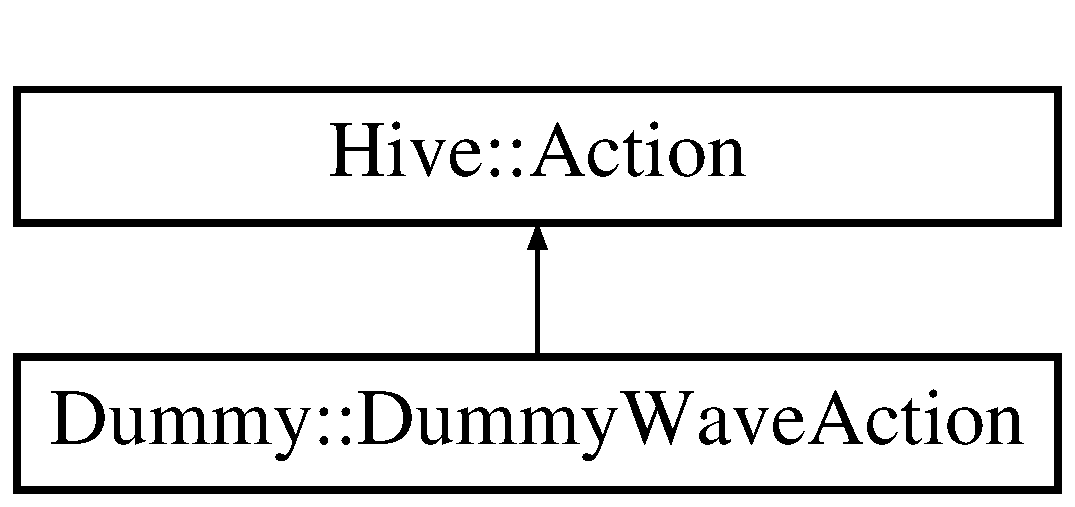
\includegraphics[height=2cm]{classDummy_1_1DummyWaveAction}
\end{center}
\end{figure}


\subsection{Detailed Description}
this is a dummy implementation of the action class 

a dummywaveaction prints out 'wave' on cerr and adds the number of waves to the agents database item ...

\begin{Desc}
\item[{\bf Todo}]error-checking whether the counter exists in the agent\end{Desc}
\begin{Desc}
\item[Author:]garrit jentsch\end{Desc}
\begin{Desc}
\item[Date:]Oct 14, 2009 last edited 10-15-2009 by garrit \end{Desc}
\subsection*{Public Member Functions}
\begin{CompactItemize}
\item 
{\bf DummyWaveAction} ()
\item 
{\bf DummyWaveAction} (int id)
\item 
void {\bf fire} ({\bf Data} $\ast$d)
\end{CompactItemize}


\subsection{Constructor \& Destructor Documentation}
\index{Dummy::DummyWaveAction@{Dummy::DummyWaveAction}!DummyWaveAction@{DummyWaveAction}}
\index{DummyWaveAction@{DummyWaveAction}!Dummy::DummyWaveAction@{Dummy::DummyWaveAction}}
\subsubsection[DummyWaveAction]{\setlength{\rightskip}{0pt plus 5cm}DummyWaveAction::DummyWaveAction ()}\label{classDummy_1_1DummyWaveAction_29c6d4182671fbe212fea9b435460f9d}


\index{Dummy::DummyWaveAction@{Dummy::DummyWaveAction}!DummyWaveAction@{DummyWaveAction}}
\index{DummyWaveAction@{DummyWaveAction}!Dummy::DummyWaveAction@{Dummy::DummyWaveAction}}
\subsubsection[DummyWaveAction]{\setlength{\rightskip}{0pt plus 5cm}DummyWaveAction::DummyWaveAction (int {\em id})}\label{classDummy_1_1DummyWaveAction_13ba34d7f3aee5436b9a196296ef13d1}




\subsection{Member Function Documentation}
\index{Dummy::DummyWaveAction@{Dummy::DummyWaveAction}!fire@{fire}}
\index{fire@{fire}!Dummy::DummyWaveAction@{Dummy::DummyWaveAction}}
\subsubsection[fire]{\setlength{\rightskip}{0pt plus 5cm}void DummyWaveAction::fire ({\bf Data} $\ast$ {\em d})\hspace{0.3cm}{\tt  [virtual]}}\label{classDummy_1_1DummyWaveAction_da12711cb5d2ff3f5df637dbb28ebeff}


executes an action \begin{Desc}
\item[Parameters:]
\begin{description}
\item[{\em d}]pointer to data-object containing the argument for the action \end{description}
\end{Desc}


Implements {\bf Hive::Action} \doxyref{}{p.}{classHive_1_1Action_b49f6239755b61cd057b7024d739e8ba}.

References Hive::Action::agent, Hive::Agent::getDatabase(), Hive::Database::getDataItem(), Hive::IntegerData::getInteger(), and Hive::Data::getType().

The documentation for this class was generated from the following files:\begin{CompactItemize}
\item 
{\bf dummywaveaction.hh}\item 
{\bf dummywaveaction.cpp}\end{CompactItemize}

\section{Hive::InputDataReader Class Reference}
\label{classHive_1_1InputDataReader}\index{Hive::InputDataReader@{Hive::InputDataReader}}
{\tt \#include $<$inputdatareader.hh$>$}



\subsection{Detailed Description}
reads input from filestream 

by introducing an input data reader class we separate the storage of a database from its use.

\begin{Desc}
\item[{\bf Todo}]Everything\end{Desc}
\begin{Desc}
\item[{\bf Bug}]unknown as of yet\end{Desc}
\begin{Desc}
\item[Author:]Garrit Jentsch\end{Desc}
\begin{Desc}
\item[Date:]Oct 13, 2009 last edited: Oct 13, 2009 by Garrit \end{Desc}
\subsection*{Public Member Functions}
\begin{CompactItemize}
\item 
{\bf InputDataReader} ()
\begin{CompactList}\small\item\em constructor \item\end{CompactList}\item 
{\bf $\sim$InputDataReader} ()
\begin{CompactList}\small\item\em destructor \item\end{CompactList}\item 
void {\bf read} (ifstream \&input)
\end{CompactItemize}
\subsection*{Protected Member Functions}
\begin{CompactItemize}
\item 
{\bf Data} $\ast$ {\bf getNextDataItem} ()
\end{CompactItemize}


\subsection{Constructor \& Destructor Documentation}
\index{Hive::InputDataReader@{Hive::InputDataReader}!InputDataReader@{InputDataReader}}
\index{InputDataReader@{InputDataReader}!Hive::InputDataReader@{Hive::InputDataReader}}
\subsubsection[InputDataReader]{\setlength{\rightskip}{0pt plus 5cm}Hive::InputDataReader::InputDataReader ()}\label{classHive_1_1InputDataReader_d9f91314addd1ffeafb4cf0907faabd2}


constructor 

\index{Hive::InputDataReader@{Hive::InputDataReader}!$\sim$InputDataReader@{$\sim$InputDataReader}}
\index{$\sim$InputDataReader@{$\sim$InputDataReader}!Hive::InputDataReader@{Hive::InputDataReader}}
\subsubsection[$\sim$InputDataReader]{\setlength{\rightskip}{0pt plus 5cm}Hive::InputDataReader::$\sim$InputDataReader ()}\label{classHive_1_1InputDataReader_d040f380f77015443f56cc45d6f99db5}


destructor 



\subsection{Member Function Documentation}
\index{Hive::InputDataReader@{Hive::InputDataReader}!read@{read}}
\index{read@{read}!Hive::InputDataReader@{Hive::InputDataReader}}
\subsubsection[read]{\setlength{\rightskip}{0pt plus 5cm}void Hive::InputDataReader::read (ifstream \& {\em input})}\label{classHive_1_1InputDataReader_69b4beee15ca8699cd49056e4cf8c319}


read data from file \begin{Desc}
\item[Parameters:]
\begin{description}
\item[{\em input}]input file stream \end{description}
\end{Desc}
\index{Hive::InputDataReader@{Hive::InputDataReader}!getNextDataItem@{getNextDataItem}}
\index{getNextDataItem@{getNextDataItem}!Hive::InputDataReader@{Hive::InputDataReader}}
\subsubsection[getNextDataItem]{\setlength{\rightskip}{0pt plus 5cm}{\bf Data}$\ast$ Hive::InputDataReader::getNextDataItem ()\hspace{0.3cm}{\tt  [protected]}}\label{classHive_1_1InputDataReader_f35864f9ba42c078b0d4fc033c64a30a}


reads the next element from the input file-stream \begin{Desc}
\item[Returns:]pointer to data element \end{Desc}


The documentation for this class was generated from the following file:\begin{CompactItemize}
\item 
{\bf inputdatareader.hh}\end{CompactItemize}

\section{Hive::InputSystemReader Class Reference}
\label{classHive_1_1InputSystemReader}\index{Hive::InputSystemReader@{Hive::InputSystemReader}}
{\tt \#include $<$inputsystemreader.hh$>$}



\subsection{Detailed Description}
abstract class for reading a system 

this class reads a system for agent setup

\begin{Desc}
\item[{\bf Todo}]everything\end{Desc}
\begin{Desc}
\item[{\bf Bug}]\end{Desc}
\begin{Desc}
\item[Author:]Garrit Jentsch and Michael Sneddon\end{Desc}
\begin{Desc}
\item[Date:]Oct 13th, 2009 last edited: 10-14-2009 by Garrit and Michael \end{Desc}


The documentation for this class was generated from the following file:\begin{CompactItemize}
\item 
{\bf inputsystemreader.hh}\end{CompactItemize}

\section{Hive::IntegerData Class Reference}
\label{classHive_1_1IntegerData}\index{Hive::IntegerData@{Hive::IntegerData}}
{\tt \#include $<$primitiveData.hh$>$}

Inheritance diagram for Hive::IntegerData::\begin{figure}[H]
\begin{center}
\leavevmode
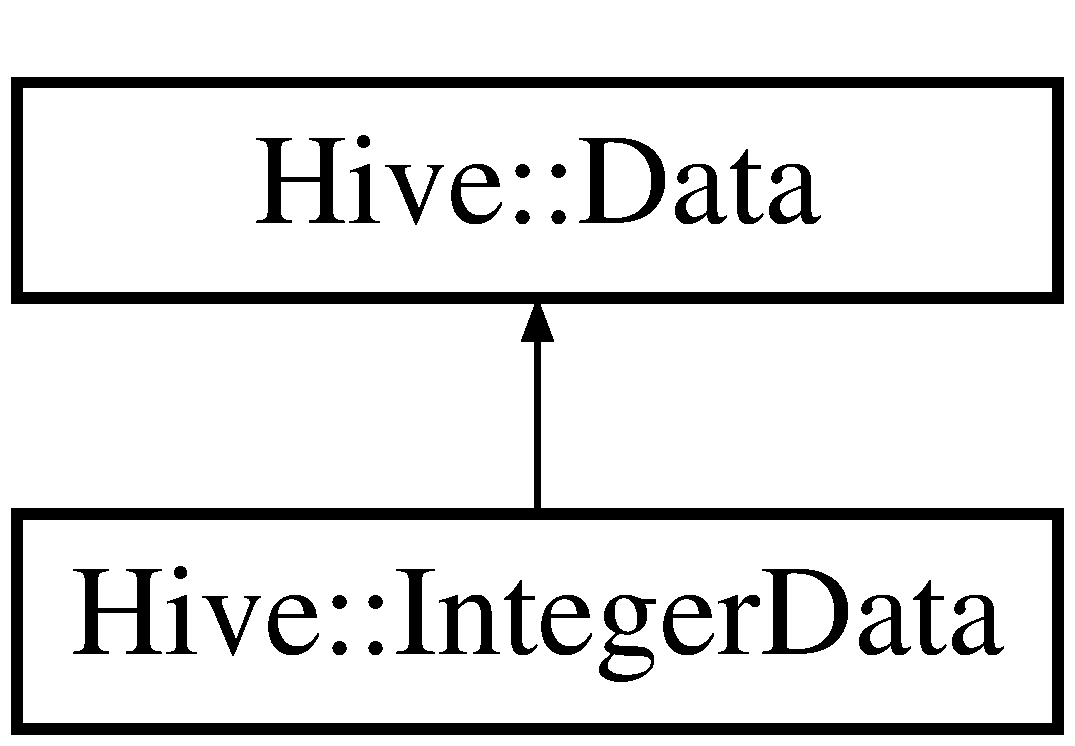
\includegraphics[height=2cm]{classHive_1_1IntegerData}
\end{center}
\end{figure}


\subsection{Detailed Description}
A data object to store integer values. 

\begin{Desc}
\item[Date:]Oct 14, 2009 Last edited: Oct 14, 2009 by Garrit and Michael \end{Desc}
\begin{Desc}
\item[Author:]Michael Sneddon \end{Desc}
\subsection*{Public Member Functions}
\begin{CompactItemize}
\item 
{\bf IntegerData} (string dataName, int value)
\begin{CompactList}\small\item\em default-constructor \item\end{CompactList}\item 
virtual {\bf $\sim$IntegerData} ()
\item 
void {\bf printContent} (ostream \&out)
\begin{CompactList}\small\item\em virtual method for print the content of a data item on sterr. \item\end{CompactList}\item 
string {\bf getDataName} () const 
\item 
int {\bf getInteger} () const 
\item 
void {\bf setInteger} (int newValue)
\end{CompactItemize}


\subsection{Constructor \& Destructor Documentation}
\index{Hive::IntegerData@{Hive::IntegerData}!IntegerData@{IntegerData}}
\index{IntegerData@{IntegerData}!Hive::IntegerData@{Hive::IntegerData}}
\subsubsection[IntegerData]{\setlength{\rightskip}{0pt plus 5cm}IntegerData::IntegerData (string {\em dataName}, \/  int {\em value})}\label{classHive_1_1IntegerData_746aec52ee5800f9d1f665c0551ac550}


default-constructor 

\index{Hive::IntegerData@{Hive::IntegerData}!$\sim$IntegerData@{$\sim$IntegerData}}
\index{$\sim$IntegerData@{$\sim$IntegerData}!Hive::IntegerData@{Hive::IntegerData}}
\subsubsection[$\sim$IntegerData]{\setlength{\rightskip}{0pt plus 5cm}virtual Hive::IntegerData::$\sim$IntegerData ()\hspace{0.3cm}{\tt  [inline, virtual]}}\label{classHive_1_1IntegerData_fe3c1be18fa73a3d0e15524e48189990}




\subsection{Member Function Documentation}
\index{Hive::IntegerData@{Hive::IntegerData}!printContent@{printContent}}
\index{printContent@{printContent}!Hive::IntegerData@{Hive::IntegerData}}
\subsubsection[printContent]{\setlength{\rightskip}{0pt plus 5cm}void IntegerData::printContent (ostream \& {\em out})\hspace{0.3cm}{\tt  [virtual]}}\label{classHive_1_1IntegerData_c8b7d3312b0335c50a0e74aa8bf6a2c0}


virtual method for print the content of a data item on sterr. 



Implements {\bf Hive::Data} \doxyref{}{p.}{classHive_1_1Data_a168edcfa6efd38fe88d72c5162fd8d1}.

References Hive::Data::datatype.\index{Hive::IntegerData@{Hive::IntegerData}!getDataName@{getDataName}}
\index{getDataName@{getDataName}!Hive::IntegerData@{Hive::IntegerData}}
\subsubsection[getDataName]{\setlength{\rightskip}{0pt plus 5cm}string Hive::IntegerData::getDataName () const\hspace{0.3cm}{\tt  [inline]}}\label{classHive_1_1IntegerData_4907987df5bd909decc6b433517fa71f}




Referenced by Dummy::DummyAgentFactory::createAgent().\index{Hive::IntegerData@{Hive::IntegerData}!getInteger@{getInteger}}
\index{getInteger@{getInteger}!Hive::IntegerData@{Hive::IntegerData}}
\subsubsection[getInteger]{\setlength{\rightskip}{0pt plus 5cm}int Hive::IntegerData::getInteger () const\hspace{0.3cm}{\tt  [inline]}}\label{classHive_1_1IntegerData_229292da4f10cb1532a311129d300889}




Referenced by Dummy::DummyWaveAction::fire().\index{Hive::IntegerData@{Hive::IntegerData}!setInteger@{setInteger}}
\index{setInteger@{setInteger}!Hive::IntegerData@{Hive::IntegerData}}
\subsubsection[setInteger]{\setlength{\rightskip}{0pt plus 5cm}void Hive::IntegerData::setInteger (int {\em newValue})\hspace{0.3cm}{\tt  [inline]}}\label{classHive_1_1IntegerData_9f99706b847cdb75a9abab0b1bb51f0b}




The documentation for this class was generated from the following files:\begin{CompactItemize}
\item 
{\bf primitiveData.hh}\item 
{\bf primitiveData.cpp}\end{CompactItemize}

\section{Hive::Message Class Reference}
\label{classHive_1_1Message}\index{Hive::Message@{Hive::Message}}
{\tt \#include $<$message.hh$>$}



\subsection{Detailed Description}
message for agent communication. 

messages are exchanged by agents to communicate with one another. with the help of a message agents tell each other which action they should take.

\begin{Desc}
\item[See also:]action\end{Desc}
\begin{Desc}
\item[{\bf Todo}]everything. how do we specify the parameters ?!\end{Desc}
\begin{Desc}
\item[{\bf Bug}]\end{Desc}
\begin{Desc}
\item[Author:]Garrit Jentsch\end{Desc}
\begin{Desc}
\item[Date:]Oct 13th, 2009 last edited: 10-14-2009 by Garrit and Michael \end{Desc}
\subsection*{Public Member Functions}
\begin{CompactItemize}
\item 
{\bf Message} ()
\begin{CompactList}\small\item\em Constructor. \item\end{CompactList}\item 
{\bf $\sim$Message} ()
\begin{CompactList}\small\item\em destructor \item\end{CompactList}\item 
int {\bf getActionId} ()
\item 
void {\bf setAction} (int a)
\item 
void {\bf setArgument} ({\bf Data} \&d)
\item 
void {\bf setArgument} ({\bf Data} $\ast$d)
\item 
void {\bf getArgument} ({\bf Data} $\ast$\&d, int i=0)
\item 
void {\bf getAllParameter} (vector$<$ {\bf Data} $\ast$ $>$ \&d)
\end{CompactItemize}


\subsection{Constructor \& Destructor Documentation}
\index{Hive::Message@{Hive::Message}!Message@{Message}}
\index{Message@{Message}!Hive::Message@{Hive::Message}}
\subsubsection[Message]{\setlength{\rightskip}{0pt plus 5cm}Message::Message ()}\label{classHive_1_1Message_4fc4f717b634e66070366cb7722d7761}


Constructor. 

\index{Hive::Message@{Hive::Message}!$\sim$Message@{$\sim$Message}}
\index{$\sim$Message@{$\sim$Message}!Hive::Message@{Hive::Message}}
\subsubsection[$\sim$Message]{\setlength{\rightskip}{0pt plus 5cm}Message::$\sim$Message ()}\label{classHive_1_1Message_3f7275462831f787a861271687bcad67}


destructor 



\subsection{Member Function Documentation}
\index{Hive::Message@{Hive::Message}!getActionId@{getActionId}}
\index{getActionId@{getActionId}!Hive::Message@{Hive::Message}}
\subsubsection[getActionId]{\setlength{\rightskip}{0pt plus 5cm}int Message::getActionId ()}\label{classHive_1_1Message_b432b3eee3b03fb5b7b25b530898fa96}


returns actionid of the action to be taken by the destination agent \begin{Desc}
\item[Returns:]actionid \end{Desc}


Referenced by Hive::Agent::evaluateMessageQueue().\index{Hive::Message@{Hive::Message}!setAction@{setAction}}
\index{setAction@{setAction}!Hive::Message@{Hive::Message}}
\subsubsection[setAction]{\setlength{\rightskip}{0pt plus 5cm}void Message::setAction (int {\em a})}\label{classHive_1_1Message_6cc1ac636810840ebeef7f78234fed93}


set action which has to be communicated \begin{Desc}
\item[Parameters:]
\begin{description}
\item[{\em a}]action to be broadcasted. \end{description}
\end{Desc}


Referenced by Dummy::DummyMessageGenerator::placeMessage().\index{Hive::Message@{Hive::Message}!setArgument@{setArgument}}
\index{setArgument@{setArgument}!Hive::Message@{Hive::Message}}
\subsubsection[setArgument]{\setlength{\rightskip}{0pt plus 5cm}void Hive::Message::setArgument ({\bf Data} \& {\em d})}\label{classHive_1_1Message_cc22028635f3bffdb5b5187e3cd3b052}


adds an arbitrary data item to the parameter list \begin{Desc}
\item[Parameters:]
\begin{description}
\item[{\em d}]data item \end{description}
\end{Desc}


Referenced by Dummy::DummyMessageGenerator::placeMessage().\index{Hive::Message@{Hive::Message}!setArgument@{setArgument}}
\index{setArgument@{setArgument}!Hive::Message@{Hive::Message}}
\subsubsection[setArgument]{\setlength{\rightskip}{0pt plus 5cm}void Message::setArgument ({\bf Data} $\ast$ {\em d})}\label{classHive_1_1Message_975ed4851d03e7ab133845f3853eb16a}


adds a pointer to an arbitrary data item to the parameter list \begin{Desc}
\item[Parameters:]
\begin{description}
\item[{\em $\ast$d}]pointer to data item \end{description}
\end{Desc}
\index{Hive::Message@{Hive::Message}!getArgument@{getArgument}}
\index{getArgument@{getArgument}!Hive::Message@{Hive::Message}}
\subsubsection[getArgument]{\setlength{\rightskip}{0pt plus 5cm}void Message::getArgument ({\bf Data} $\ast$\& {\em d}, \/  int {\em i} = {\tt 0})}\label{classHive_1_1Message_29285c0e99174654d44ca2b7388ad9f5}


return data item at a certain position \begin{Desc}
\item[Parameters:]
\begin{description}
\item[{\em $\ast$d}]return parameter \item[{\em i}]position \end{description}
\end{Desc}


Referenced by Hive::Agent::evaluateMessageQueue().\index{Hive::Message@{Hive::Message}!getAllParameter@{getAllParameter}}
\index{getAllParameter@{getAllParameter}!Hive::Message@{Hive::Message}}
\subsubsection[getAllParameter]{\setlength{\rightskip}{0pt plus 5cm}void Hive::Message::getAllParameter (vector$<$ {\bf Data} $\ast$ $>$ \& {\em d})}\label{classHive_1_1Message_172c036ad596e7cd92892b5c318d0ff9}


return data item vector \begin{Desc}
\item[Parameters:]
\begin{description}
\item[{\em $\ast$$\ast$d}]return parameter \end{description}
\end{Desc}


The documentation for this class was generated from the following files:\begin{CompactItemize}
\item 
{\bf message.hh}\item 
{\bf message.cpp}\end{CompactItemize}

\section{Hive::MessageGenerator Class Reference}
\label{classHive_1_1MessageGenerator}\index{Hive::MessageGenerator@{Hive::MessageGenerator}}
{\tt \#include $<$messagegenerator.hh$>$}

Inheritance diagram for Hive::MessageGenerator::\begin{figure}[H]
\begin{center}
\leavevmode
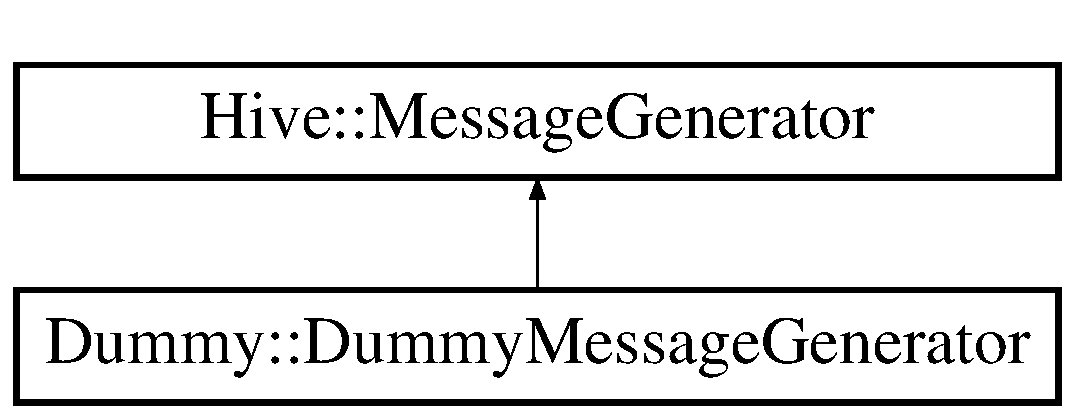
\includegraphics[height=2cm]{classHive_1_1MessageGenerator}
\end{center}
\end{figure}
\subsection*{Public Member Functions}
\begin{CompactItemize}
\item 
{\bf MessageGenerator} ()
\begin{CompactList}\small\item\em default constructor \item\end{CompactList}\item 
{\bf MessageGenerator} ({\bf Agent} $\ast$ag)
\item 
virtual {\bf $\sim$MessageGenerator} ()
\begin{CompactList}\small\item\em destructor \item\end{CompactList}\item 
virtual void {\bf placeMessage} ()=0
\end{CompactItemize}
\subsection*{Protected Attributes}
\begin{CompactItemize}
\item 
{\bf Agent} $\ast$ {\bf source}
\begin{CompactList}\small\item\em pointer to agent that generates the message \item\end{CompactList}\end{CompactItemize}


\subsection{Constructor \& Destructor Documentation}
\index{Hive::MessageGenerator@{Hive::MessageGenerator}!MessageGenerator@{MessageGenerator}}
\index{MessageGenerator@{MessageGenerator}!Hive::MessageGenerator@{Hive::MessageGenerator}}
\subsubsection[MessageGenerator]{\setlength{\rightskip}{0pt plus 5cm}Hive::MessageGenerator::MessageGenerator ()\hspace{0.3cm}{\tt  [inline]}}\label{classHive_1_1MessageGenerator_151d85b04a90038bd7475e02ecf08335}


default constructor 

\index{Hive::MessageGenerator@{Hive::MessageGenerator}!MessageGenerator@{MessageGenerator}}
\index{MessageGenerator@{MessageGenerator}!Hive::MessageGenerator@{Hive::MessageGenerator}}
\subsubsection[MessageGenerator]{\setlength{\rightskip}{0pt plus 5cm}Hive::MessageGenerator::MessageGenerator ({\bf Agent} $\ast$ {\em ag})\hspace{0.3cm}{\tt  [inline]}}\label{classHive_1_1MessageGenerator_d3db0022514a56ba1fa69850bb060989}


construct \begin{Desc}
\item[Parameters:]
\begin{description}
\item[{\em pointer}]to source agent \end{description}
\end{Desc}


References source.\index{Hive::MessageGenerator@{Hive::MessageGenerator}!$\sim$MessageGenerator@{$\sim$MessageGenerator}}
\index{$\sim$MessageGenerator@{$\sim$MessageGenerator}!Hive::MessageGenerator@{Hive::MessageGenerator}}
\subsubsection[$\sim$MessageGenerator]{\setlength{\rightskip}{0pt plus 5cm}virtual Hive::MessageGenerator::$\sim$MessageGenerator ()\hspace{0.3cm}{\tt  [inline, virtual]}}\label{classHive_1_1MessageGenerator_0dc07ead2cd7181415ca414e2992d77b}


destructor 



\subsection{Member Function Documentation}
\index{Hive::MessageGenerator@{Hive::MessageGenerator}!placeMessage@{placeMessage}}
\index{placeMessage@{placeMessage}!Hive::MessageGenerator@{Hive::MessageGenerator}}
\subsubsection[placeMessage]{\setlength{\rightskip}{0pt plus 5cm}virtual void Hive::MessageGenerator::placeMessage ()\hspace{0.3cm}{\tt  [pure virtual]}}\label{classHive_1_1MessageGenerator_874d881a3aeff02ca53391714f659a20}


generate message and puts it into the outbox of the source agent 

Implemented in {\bf Dummy::DummyMessageGenerator} \doxyref{}{p.}{classDummy_1_1DummyMessageGenerator_5a7af3c76d74a53211e440fc86514d0c}.

\subsection{Member Data Documentation}
\index{Hive::MessageGenerator@{Hive::MessageGenerator}!source@{source}}
\index{source@{source}!Hive::MessageGenerator@{Hive::MessageGenerator}}
\subsubsection[source]{\setlength{\rightskip}{0pt plus 5cm}{\bf Agent}$\ast$ {\bf Hive::MessageGenerator::source}\hspace{0.3cm}{\tt  [protected]}}\label{classHive_1_1MessageGenerator_e2567828ed7b3d9b57a5cc3a77f90075}


pointer to agent that generates the message 



Referenced by MessageGenerator(), and Dummy::DummyMessageGenerator::placeMessage().

The documentation for this class was generated from the following file:\begin{CompactItemize}
\item 
{\bf messagegenerator.hh}\end{CompactItemize}

\section{MTRand Class Reference}
\label{classMTRand}\index{MTRand@{MTRand}}
{\tt \#include $<$mtrand.h$>$}

Inheritance diagram for MTRand::\begin{figure}[H]
\begin{center}
\leavevmode
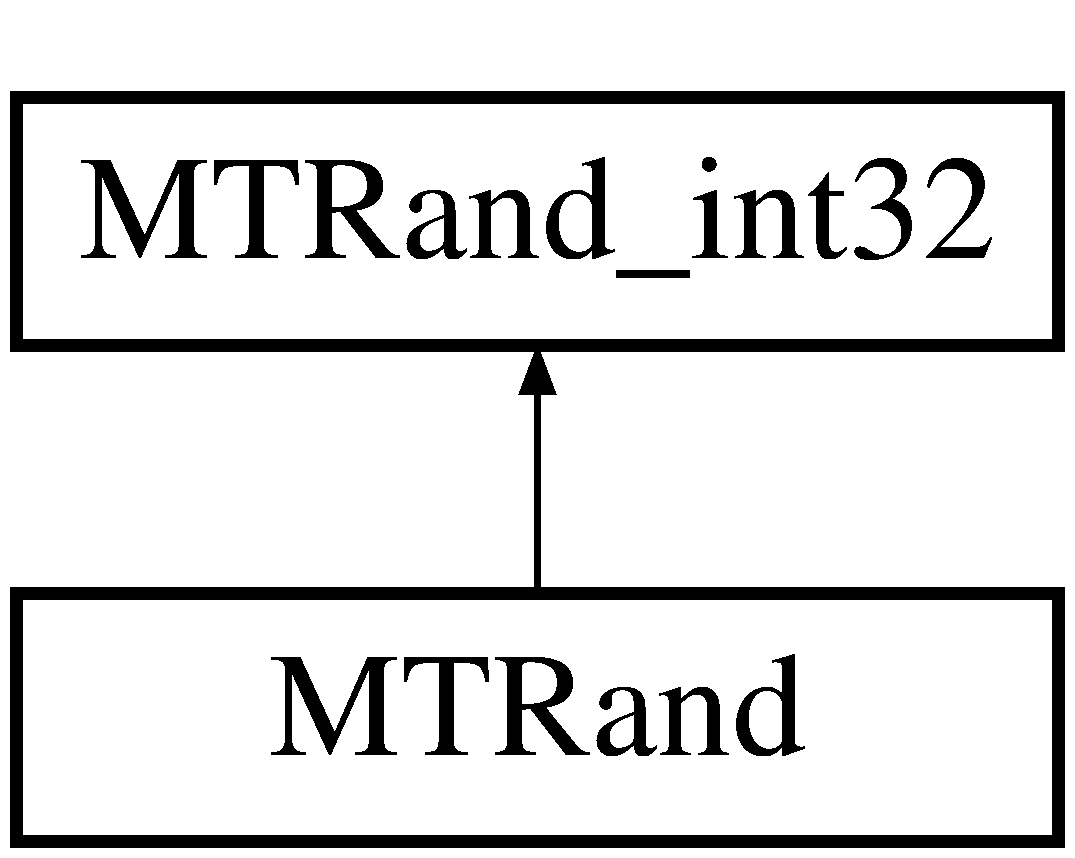
\includegraphics[height=2cm]{classMTRand}
\end{center}
\end{figure}
\subsection*{Public Member Functions}
\begin{CompactItemize}
\item 
{\bf MTRand} ()
\item 
{\bf MTRand} (unsigned long seed)
\item 
{\bf MTRand} (const unsigned long $\ast$seed, int size)
\item 
{\bf $\sim$MTRand} ()
\item 
double {\bf operator()} ()
\end{CompactItemize}


\subsection{Constructor \& Destructor Documentation}
\index{MTRand@{MTRand}!MTRand@{MTRand}}
\index{MTRand@{MTRand}!MTRand@{MTRand}}
\subsubsection[MTRand]{\setlength{\rightskip}{0pt plus 5cm}MTRand::MTRand ()\hspace{0.3cm}{\tt  [inline]}}\label{classMTRand_265dc65546e26073c0d5f8787b045a1d}


\index{MTRand@{MTRand}!MTRand@{MTRand}}
\index{MTRand@{MTRand}!MTRand@{MTRand}}
\subsubsection[MTRand]{\setlength{\rightskip}{0pt plus 5cm}MTRand::MTRand (unsigned long {\em seed})\hspace{0.3cm}{\tt  [inline]}}\label{classMTRand_2c88736896bcbdb54bcdd7a0026720d5}


\index{MTRand@{MTRand}!MTRand@{MTRand}}
\index{MTRand@{MTRand}!MTRand@{MTRand}}
\subsubsection[MTRand]{\setlength{\rightskip}{0pt plus 5cm}MTRand::MTRand (const unsigned long $\ast$ {\em seed}, \/  int {\em size})\hspace{0.3cm}{\tt  [inline]}}\label{classMTRand_6075a3beacdfb8e4cf48d9fb56cc193a}


\index{MTRand@{MTRand}!$\sim$MTRand@{$\sim$MTRand}}
\index{$\sim$MTRand@{$\sim$MTRand}!MTRand@{MTRand}}
\subsubsection[$\sim$MTRand]{\setlength{\rightskip}{0pt plus 5cm}MTRand::$\sim$MTRand ()\hspace{0.3cm}{\tt  [inline]}}\label{classMTRand_8c276546a41ae350dc9efc5e9c10a261}




\subsection{Member Function Documentation}
\index{MTRand@{MTRand}!operator()@{operator()}}
\index{operator()@{operator()}!MTRand@{MTRand}}
\subsubsection[operator()]{\setlength{\rightskip}{0pt plus 5cm}double MTRand::operator() ()\hspace{0.3cm}{\tt  [inline]}}\label{classMTRand_bbb87a08d622d58fdee0eea4cb5471a0}




Reimplemented from {\bf MTRand\_\-int32} \doxyref{}{p.}{classMTRand__int32_d7fe22190d0411c6dac8e6f471633aa4}.

References MTRand\_\-int32::rand\_\-int32().

The documentation for this class was generated from the following file:\begin{CompactItemize}
\item 
{\bf mtrand.h}\end{CompactItemize}

\section{MTRand53 Class Reference}
\label{classMTRand53}\index{MTRand53@{MTRand53}}
{\tt \#include $<$mtrand.h$>$}

Inheritance diagram for MTRand53::\begin{figure}[H]
\begin{center}
\leavevmode
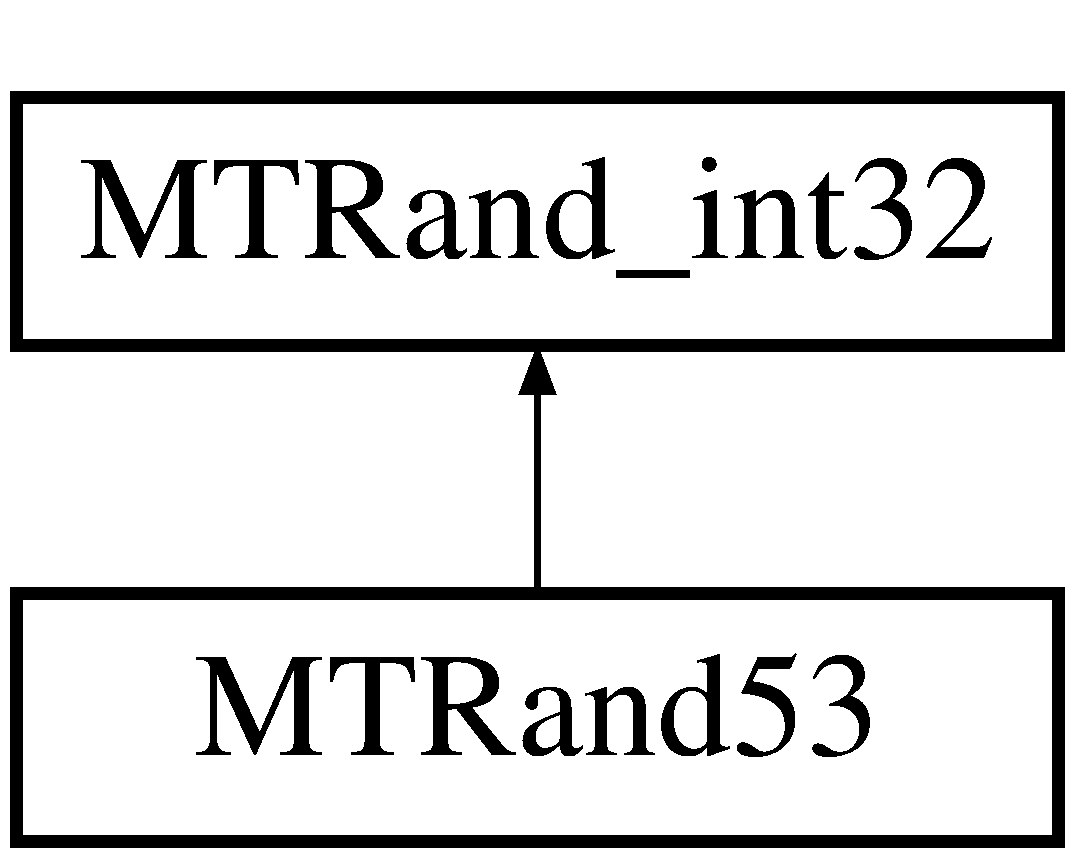
\includegraphics[height=2cm]{classMTRand53}
\end{center}
\end{figure}
\subsection*{Public Member Functions}
\begin{CompactItemize}
\item 
{\bf MTRand53} ()
\item 
{\bf MTRand53} (unsigned long seed)
\item 
{\bf MTRand53} (const unsigned long $\ast$seed, int size)
\item 
{\bf $\sim$MTRand53} ()
\item 
double {\bf operator()} ()
\end{CompactItemize}


\subsection{Constructor \& Destructor Documentation}
\index{MTRand53@{MTRand53}!MTRand53@{MTRand53}}
\index{MTRand53@{MTRand53}!MTRand53@{MTRand53}}
\subsubsection[MTRand53]{\setlength{\rightskip}{0pt plus 5cm}MTRand53::MTRand53 ()\hspace{0.3cm}{\tt  [inline]}}\label{classMTRand53_24711c9e6e5ee72715f34515d1f1939a}


\index{MTRand53@{MTRand53}!MTRand53@{MTRand53}}
\index{MTRand53@{MTRand53}!MTRand53@{MTRand53}}
\subsubsection[MTRand53]{\setlength{\rightskip}{0pt plus 5cm}MTRand53::MTRand53 (unsigned long {\em seed})\hspace{0.3cm}{\tt  [inline]}}\label{classMTRand53_d800887e15d4095f22facdb67f270c5e}


\index{MTRand53@{MTRand53}!MTRand53@{MTRand53}}
\index{MTRand53@{MTRand53}!MTRand53@{MTRand53}}
\subsubsection[MTRand53]{\setlength{\rightskip}{0pt plus 5cm}MTRand53::MTRand53 (const unsigned long $\ast$ {\em seed}, \/  int {\em size})\hspace{0.3cm}{\tt  [inline]}}\label{classMTRand53_c77b190d3ac27adea2d2c6c2ce2347c3}


\index{MTRand53@{MTRand53}!$\sim$MTRand53@{$\sim$MTRand53}}
\index{$\sim$MTRand53@{$\sim$MTRand53}!MTRand53@{MTRand53}}
\subsubsection[$\sim$MTRand53]{\setlength{\rightskip}{0pt plus 5cm}MTRand53::$\sim$MTRand53 ()\hspace{0.3cm}{\tt  [inline]}}\label{classMTRand53_947a6a7afd0c8a17612cda3faa705a75}




\subsection{Member Function Documentation}
\index{MTRand53@{MTRand53}!operator()@{operator()}}
\index{operator()@{operator()}!MTRand53@{MTRand53}}
\subsubsection[operator()]{\setlength{\rightskip}{0pt plus 5cm}double MTRand53::operator() ()\hspace{0.3cm}{\tt  [inline]}}\label{classMTRand53_b6657cb5349f39bc4553d3a970458b45}




Reimplemented from {\bf MTRand\_\-int32} \doxyref{}{p.}{classMTRand__int32_d7fe22190d0411c6dac8e6f471633aa4}.

References MTRand\_\-int32::rand\_\-int32().

The documentation for this class was generated from the following file:\begin{CompactItemize}
\item 
{\bf mtrand.h}\end{CompactItemize}

\section{MTRand\_\-closed Class Reference}
\label{classMTRand__closed}\index{MTRand\_\-closed@{MTRand\_\-closed}}
{\tt \#include $<$mtrand.h$>$}

Inheritance diagram for MTRand\_\-closed::\begin{figure}[H]
\begin{center}
\leavevmode
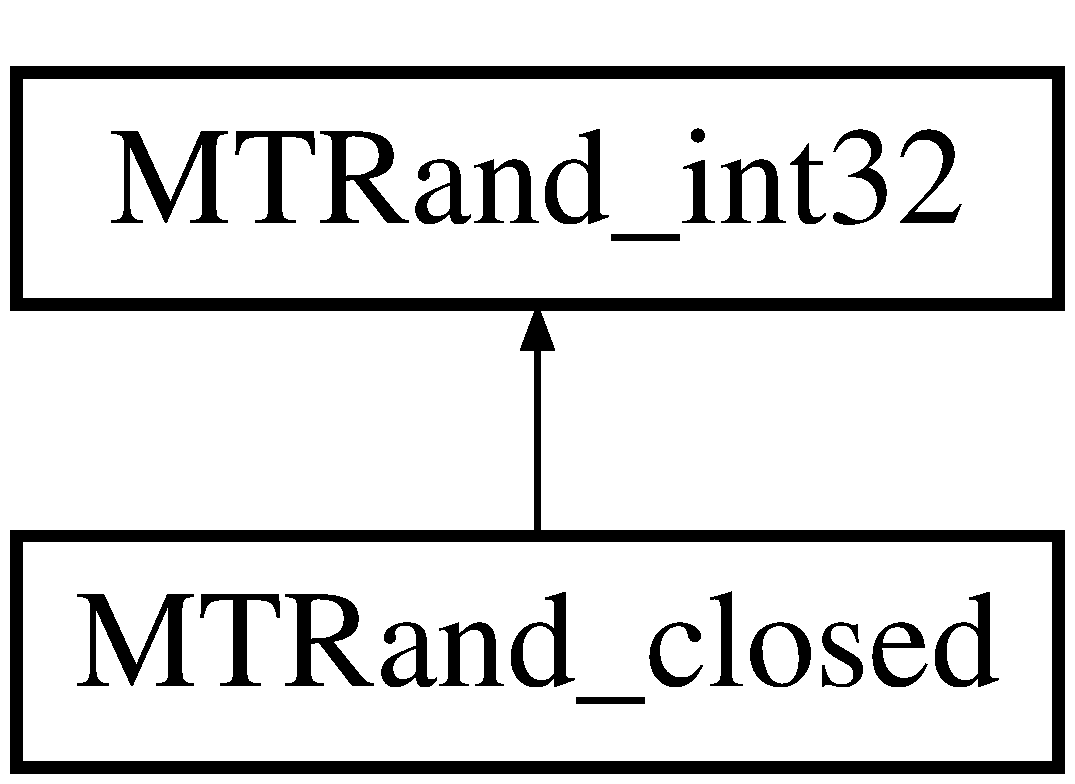
\includegraphics[height=2cm]{classMTRand__closed}
\end{center}
\end{figure}
\subsection*{Public Member Functions}
\begin{CompactItemize}
\item 
{\bf MTRand\_\-closed} ()
\item 
{\bf MTRand\_\-closed} (unsigned long seed)
\item 
{\bf MTRand\_\-closed} (const unsigned long $\ast$seed, int size)
\item 
{\bf $\sim$MTRand\_\-closed} ()
\item 
double {\bf operator()} ()
\end{CompactItemize}


\subsection{Constructor \& Destructor Documentation}
\index{MTRand\_\-closed@{MTRand\_\-closed}!MTRand\_\-closed@{MTRand\_\-closed}}
\index{MTRand\_\-closed@{MTRand\_\-closed}!MTRand_closed@{MTRand\_\-closed}}
\subsubsection[MTRand\_\-closed]{\setlength{\rightskip}{0pt plus 5cm}MTRand\_\-closed::MTRand\_\-closed ()\hspace{0.3cm}{\tt  [inline]}}\label{classMTRand__closed_09b3b21b3cb35d04f2b6c290a817b2e8}


\index{MTRand\_\-closed@{MTRand\_\-closed}!MTRand\_\-closed@{MTRand\_\-closed}}
\index{MTRand\_\-closed@{MTRand\_\-closed}!MTRand_closed@{MTRand\_\-closed}}
\subsubsection[MTRand\_\-closed]{\setlength{\rightskip}{0pt plus 5cm}MTRand\_\-closed::MTRand\_\-closed (unsigned long {\em seed})\hspace{0.3cm}{\tt  [inline]}}\label{classMTRand__closed_d5dc83250b16f22d4693a18b51816271}


\index{MTRand\_\-closed@{MTRand\_\-closed}!MTRand\_\-closed@{MTRand\_\-closed}}
\index{MTRand\_\-closed@{MTRand\_\-closed}!MTRand_closed@{MTRand\_\-closed}}
\subsubsection[MTRand\_\-closed]{\setlength{\rightskip}{0pt plus 5cm}MTRand\_\-closed::MTRand\_\-closed (const unsigned long $\ast$ {\em seed}, \/  int {\em size})\hspace{0.3cm}{\tt  [inline]}}\label{classMTRand__closed_37e322f97253b7013823a267bcfe82d1}


\index{MTRand\_\-closed@{MTRand\_\-closed}!$\sim$MTRand\_\-closed@{$\sim$MTRand\_\-closed}}
\index{$\sim$MTRand\_\-closed@{$\sim$MTRand\_\-closed}!MTRand_closed@{MTRand\_\-closed}}
\subsubsection[$\sim$MTRand\_\-closed]{\setlength{\rightskip}{0pt plus 5cm}MTRand\_\-closed::$\sim$MTRand\_\-closed ()\hspace{0.3cm}{\tt  [inline]}}\label{classMTRand__closed_46567ee841b5f54b305ac051ac837a8c}




\subsection{Member Function Documentation}
\index{MTRand\_\-closed@{MTRand\_\-closed}!operator()@{operator()}}
\index{operator()@{operator()}!MTRand_closed@{MTRand\_\-closed}}
\subsubsection[operator()]{\setlength{\rightskip}{0pt plus 5cm}double MTRand\_\-closed::operator() ()\hspace{0.3cm}{\tt  [inline]}}\label{classMTRand__closed_d0c535263b63c95029523183f672f62d}




Reimplemented from {\bf MTRand\_\-int32} \doxyref{}{p.}{classMTRand__int32_d7fe22190d0411c6dac8e6f471633aa4}.

References MTRand\_\-int32::rand\_\-int32().

The documentation for this class was generated from the following file:\begin{CompactItemize}
\item 
{\bf mtrand.h}\end{CompactItemize}

\section{MTRand\_\-int32 Class Reference}
\label{classMTRand__int32}\index{MTRand\_\-int32@{MTRand\_\-int32}}
{\tt \#include $<$mtrand.h$>$}

Inheritance diagram for MTRand\_\-int32::\begin{figure}[H]
\begin{center}
\leavevmode
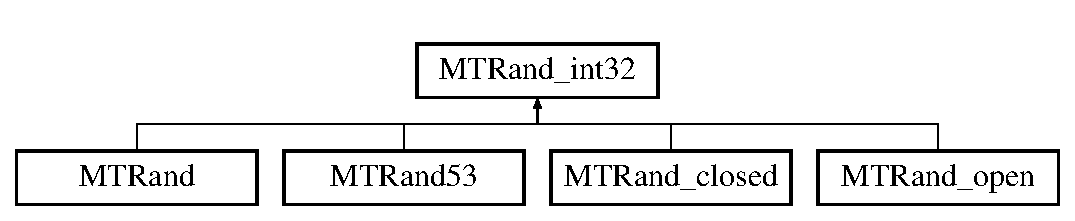
\includegraphics[height=2cm]{classMTRand__int32}
\end{center}
\end{figure}
\subsection*{Public Member Functions}
\begin{CompactItemize}
\item 
{\bf MTRand\_\-int32} ()
\item 
{\bf MTRand\_\-int32} (unsigned long s)
\item 
{\bf MTRand\_\-int32} (const unsigned long $\ast$array, int size)
\item 
void {\bf seed} (unsigned long)
\item 
void {\bf seed} (const unsigned long $\ast$, int size)
\item 
unsigned long {\bf operator()} ()
\item 
virtual {\bf $\sim$MTRand\_\-int32} ()
\end{CompactItemize}
\subsection*{Protected Member Functions}
\begin{CompactItemize}
\item 
unsigned long {\bf rand\_\-int32} ()
\end{CompactItemize}


\subsection{Constructor \& Destructor Documentation}
\index{MTRand\_\-int32@{MTRand\_\-int32}!MTRand\_\-int32@{MTRand\_\-int32}}
\index{MTRand\_\-int32@{MTRand\_\-int32}!MTRand_int32@{MTRand\_\-int32}}
\subsubsection[MTRand\_\-int32]{\setlength{\rightskip}{0pt plus 5cm}MTRand\_\-int32::MTRand\_\-int32 ()\hspace{0.3cm}{\tt  [inline]}}\label{classMTRand__int32_034f223c086f5368bd220b02f2cc12a8}




References seed().\index{MTRand\_\-int32@{MTRand\_\-int32}!MTRand\_\-int32@{MTRand\_\-int32}}
\index{MTRand\_\-int32@{MTRand\_\-int32}!MTRand_int32@{MTRand\_\-int32}}
\subsubsection[MTRand\_\-int32]{\setlength{\rightskip}{0pt plus 5cm}MTRand\_\-int32::MTRand\_\-int32 (unsigned long {\em s})\hspace{0.3cm}{\tt  [inline]}}\label{classMTRand__int32_d30f7c63a6f1fb3c3b76b8ce6ffa0206}




References seed().\index{MTRand\_\-int32@{MTRand\_\-int32}!MTRand\_\-int32@{MTRand\_\-int32}}
\index{MTRand\_\-int32@{MTRand\_\-int32}!MTRand_int32@{MTRand\_\-int32}}
\subsubsection[MTRand\_\-int32]{\setlength{\rightskip}{0pt plus 5cm}MTRand\_\-int32::MTRand\_\-int32 (const unsigned long $\ast$ {\em array}, \/  int {\em size})\hspace{0.3cm}{\tt  [inline]}}\label{classMTRand__int32_19acddb3910a7282517b2ffc398b92b4}




References seed().\index{MTRand\_\-int32@{MTRand\_\-int32}!$\sim$MTRand\_\-int32@{$\sim$MTRand\_\-int32}}
\index{$\sim$MTRand\_\-int32@{$\sim$MTRand\_\-int32}!MTRand_int32@{MTRand\_\-int32}}
\subsubsection[$\sim$MTRand\_\-int32]{\setlength{\rightskip}{0pt plus 5cm}virtual MTRand\_\-int32::$\sim$MTRand\_\-int32 ()\hspace{0.3cm}{\tt  [inline, virtual]}}\label{classMTRand__int32_364900abea0758d070ce89922159923a}




\subsection{Member Function Documentation}
\index{MTRand\_\-int32@{MTRand\_\-int32}!seed@{seed}}
\index{seed@{seed}!MTRand_int32@{MTRand\_\-int32}}
\subsubsection[seed]{\setlength{\rightskip}{0pt plus 5cm}void MTRand\_\-int32::seed (unsigned long {\em s})}\label{classMTRand__int32_0c57076fe30358e0700a7ce1baa0ea27}




Referenced by MTRand\_\-int32(), Util::RANDOM(), Util::RANDOM\_\-CLOSED(), Util::RANDOM\_\-GAUSSIAN(), Util::RANDOM\_\-INT(), seed(), and Util::SEED\_\-RANDOM().\index{MTRand\_\-int32@{MTRand\_\-int32}!seed@{seed}}
\index{seed@{seed}!MTRand_int32@{MTRand\_\-int32}}
\subsubsection[seed]{\setlength{\rightskip}{0pt plus 5cm}void MTRand\_\-int32::seed (const unsigned long $\ast$ {\em array}, \/  int {\em size})}\label{classMTRand__int32_3cabc1e3445716236a570ffd2f69686d}




References seed().\index{MTRand\_\-int32@{MTRand\_\-int32}!operator()@{operator()}}
\index{operator()@{operator()}!MTRand_int32@{MTRand\_\-int32}}
\subsubsection[operator()]{\setlength{\rightskip}{0pt plus 5cm}unsigned long MTRand\_\-int32::operator() ()\hspace{0.3cm}{\tt  [inline]}}\label{classMTRand__int32_d7fe22190d0411c6dac8e6f471633aa4}




Reimplemented in {\bf MTRand} \doxyref{}{p.}{classMTRand_bbb87a08d622d58fdee0eea4cb5471a0}, {\bf MTRand\_\-closed} \doxyref{}{p.}{classMTRand__closed_d0c535263b63c95029523183f672f62d}, {\bf MTRand\_\-open} \doxyref{}{p.}{classMTRand__open_c408aa400ca59fc2afc888d88f98d807}, and {\bf MTRand53} \doxyref{}{p.}{classMTRand53_b6657cb5349f39bc4553d3a970458b45}.

References rand\_\-int32().\index{MTRand\_\-int32@{MTRand\_\-int32}!rand\_\-int32@{rand\_\-int32}}
\index{rand\_\-int32@{rand\_\-int32}!MTRand_int32@{MTRand\_\-int32}}
\subsubsection[rand\_\-int32]{\setlength{\rightskip}{0pt plus 5cm}unsigned long MTRand\_\-int32::rand\_\-int32 ()\hspace{0.3cm}{\tt  [inline, protected]}}\label{classMTRand__int32_bacdfa346255baeac69d29bb57f29b22}




Referenced by MTRand53::operator()(), MTRand\_\-open::operator()(), MTRand\_\-closed::operator()(), MTRand::operator()(), and operator()().

The documentation for this class was generated from the following files:\begin{CompactItemize}
\item 
{\bf mtrand.h}\item 
{\bf mtrand.cpp}\end{CompactItemize}

\section{MTRand\_\-open Class Reference}
\label{classMTRand__open}\index{MTRand\_\-open@{MTRand\_\-open}}
{\tt \#include $<$mtrand.h$>$}

Inheritance diagram for MTRand\_\-open::\begin{figure}[H]
\begin{center}
\leavevmode
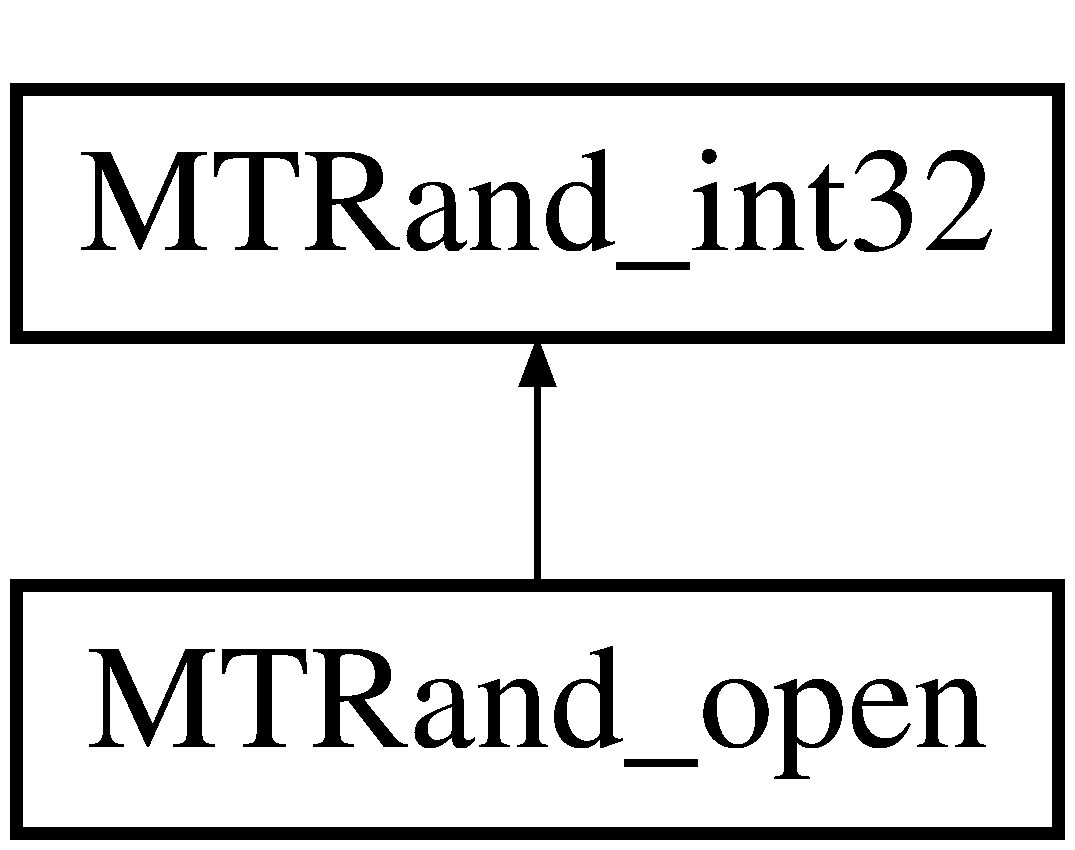
\includegraphics[height=2cm]{classMTRand__open}
\end{center}
\end{figure}
\subsection*{Public Member Functions}
\begin{CompactItemize}
\item 
{\bf MTRand\_\-open} ()
\item 
{\bf MTRand\_\-open} (unsigned long seed)
\item 
{\bf MTRand\_\-open} (const unsigned long $\ast$seed, int size)
\item 
{\bf $\sim$MTRand\_\-open} ()
\item 
double {\bf operator()} ()
\end{CompactItemize}


\subsection{Constructor \& Destructor Documentation}
\index{MTRand\_\-open@{MTRand\_\-open}!MTRand\_\-open@{MTRand\_\-open}}
\index{MTRand\_\-open@{MTRand\_\-open}!MTRand_open@{MTRand\_\-open}}
\subsubsection[MTRand\_\-open]{\setlength{\rightskip}{0pt plus 5cm}MTRand\_\-open::MTRand\_\-open ()\hspace{0.3cm}{\tt  [inline]}}\label{classMTRand__open_58140b54564be39382da163954177389}


\index{MTRand\_\-open@{MTRand\_\-open}!MTRand\_\-open@{MTRand\_\-open}}
\index{MTRand\_\-open@{MTRand\_\-open}!MTRand_open@{MTRand\_\-open}}
\subsubsection[MTRand\_\-open]{\setlength{\rightskip}{0pt plus 5cm}MTRand\_\-open::MTRand\_\-open (unsigned long {\em seed})\hspace{0.3cm}{\tt  [inline]}}\label{classMTRand__open_1f55ebc1052f5343f8d6e08a752ef957}


\index{MTRand\_\-open@{MTRand\_\-open}!MTRand\_\-open@{MTRand\_\-open}}
\index{MTRand\_\-open@{MTRand\_\-open}!MTRand_open@{MTRand\_\-open}}
\subsubsection[MTRand\_\-open]{\setlength{\rightskip}{0pt plus 5cm}MTRand\_\-open::MTRand\_\-open (const unsigned long $\ast$ {\em seed}, \/  int {\em size})\hspace{0.3cm}{\tt  [inline]}}\label{classMTRand__open_0216992f4dfa5acf22ee8c585eeac488}


\index{MTRand\_\-open@{MTRand\_\-open}!$\sim$MTRand\_\-open@{$\sim$MTRand\_\-open}}
\index{$\sim$MTRand\_\-open@{$\sim$MTRand\_\-open}!MTRand_open@{MTRand\_\-open}}
\subsubsection[$\sim$MTRand\_\-open]{\setlength{\rightskip}{0pt plus 5cm}MTRand\_\-open::$\sim$MTRand\_\-open ()\hspace{0.3cm}{\tt  [inline]}}\label{classMTRand__open_4f4774b5d9b79972dedaec984b248581}




\subsection{Member Function Documentation}
\index{MTRand\_\-open@{MTRand\_\-open}!operator()@{operator()}}
\index{operator()@{operator()}!MTRand_open@{MTRand\_\-open}}
\subsubsection[operator()]{\setlength{\rightskip}{0pt plus 5cm}double MTRand\_\-open::operator() ()\hspace{0.3cm}{\tt  [inline]}}\label{classMTRand__open_c408aa400ca59fc2afc888d88f98d807}




Reimplemented from {\bf MTRand\_\-int32} \doxyref{}{p.}{classMTRand__int32_d7fe22190d0411c6dac8e6f471633aa4}.

References MTRand\_\-int32::rand\_\-int32().

The documentation for this class was generated from the following file:\begin{CompactItemize}
\item 
{\bf mtrand.h}\end{CompactItemize}

\section{Hive::OutputWriter Class Reference}
\label{classHive_1_1OutputWriter}\index{Hive::OutputWriter@{Hive::OutputWriter}}
{\tt \#include $<$outputwriter.hh$>$}

\subsection*{Public Member Functions}
\begin{CompactItemize}
\item 
{\bf OutputWriter} ()
\begin{CompactList}\small\item\em constructor \item\end{CompactList}\item 
{\bf $\sim$OutputWriter} ()
\begin{CompactList}\small\item\em destructor \item\end{CompactList}\item 
void {\bf dumbDatabase} ()
\item 
void {\bf setDatabase} ({\bf Database} $\ast$db)
\item 
void {\bf setOutputFileStream} (ofstream \&output)
\end{CompactItemize}
\subsection*{Protected Member Functions}
\begin{CompactItemize}
\item 
void {\bf outputNextItem} ()
\end{CompactItemize}


\subsection{Constructor \& Destructor Documentation}
\index{Hive::OutputWriter@{Hive::OutputWriter}!OutputWriter@{OutputWriter}}
\index{OutputWriter@{OutputWriter}!Hive::OutputWriter@{Hive::OutputWriter}}
\subsubsection[OutputWriter]{\setlength{\rightskip}{0pt plus 5cm}Hive::OutputWriter::OutputWriter ()}\label{classHive_1_1OutputWriter_abf751a6ebd05751a4a3b19e994eb265}


constructor 

\index{Hive::OutputWriter@{Hive::OutputWriter}!$\sim$OutputWriter@{$\sim$OutputWriter}}
\index{$\sim$OutputWriter@{$\sim$OutputWriter}!Hive::OutputWriter@{Hive::OutputWriter}}
\subsubsection[$\sim$OutputWriter]{\setlength{\rightskip}{0pt plus 5cm}Hive::OutputWriter::$\sim$OutputWriter ()}\label{classHive_1_1OutputWriter_062ec1fa9360b0030f6586b8267cf977}


destructor 



\subsection{Member Function Documentation}
\index{Hive::OutputWriter@{Hive::OutputWriter}!dumbDatabase@{dumbDatabase}}
\index{dumbDatabase@{dumbDatabase}!Hive::OutputWriter@{Hive::OutputWriter}}
\subsubsection[dumbDatabase]{\setlength{\rightskip}{0pt plus 5cm}void Hive::OutputWriter::dumbDatabase ()}\label{classHive_1_1OutputWriter_6a62b1a132128de629b8609d3e471cbf}


dumb database \index{Hive::OutputWriter@{Hive::OutputWriter}!setDatabase@{setDatabase}}
\index{setDatabase@{setDatabase}!Hive::OutputWriter@{Hive::OutputWriter}}
\subsubsection[setDatabase]{\setlength{\rightskip}{0pt plus 5cm}void Hive::OutputWriter::setDatabase ({\bf Database} $\ast$ {\em db})}\label{classHive_1_1OutputWriter_13533399b709ee1451862915dca44f89}


give database to outputwriter \begin{Desc}
\item[Parameters:]
\begin{description}
\item[{\em db}]pointer to database \end{description}
\end{Desc}
\index{Hive::OutputWriter@{Hive::OutputWriter}!setOutputFileStream@{setOutputFileStream}}
\index{setOutputFileStream@{setOutputFileStream}!Hive::OutputWriter@{Hive::OutputWriter}}
\subsubsection[setOutputFileStream]{\setlength{\rightskip}{0pt plus 5cm}void Hive::OutputWriter::setOutputFileStream (ofstream \& {\em output})}\label{classHive_1_1OutputWriter_1f38a4e3b701abc5811a20370af27a08}


give outputfile to outputwriter \begin{Desc}
\item[Parameters:]
\begin{description}
\item[{\em output}]output filestream \end{description}
\end{Desc}
\index{Hive::OutputWriter@{Hive::OutputWriter}!outputNextItem@{outputNextItem}}
\index{outputNextItem@{outputNextItem}!Hive::OutputWriter@{Hive::OutputWriter}}
\subsubsection[outputNextItem]{\setlength{\rightskip}{0pt plus 5cm}void Hive::OutputWriter::outputNextItem ()\hspace{0.3cm}{\tt  [protected]}}\label{classHive_1_1OutputWriter_ba89dae1ca1d31bf91d21731580fe03a}


outputs items of the database 

The documentation for this class was generated from the following file:\begin{CompactItemize}
\item 
{\bf outputwriter.hh}\end{CompactItemize}

\section{mu::Parser Class Reference}
\label{classmu_1_1Parser}\index{mu::Parser@{mu::Parser}}
{\tt \#include $<$muParser.h$>$}

Inheritance diagram for mu::Parser::\begin{figure}[H]
\begin{center}
\leavevmode
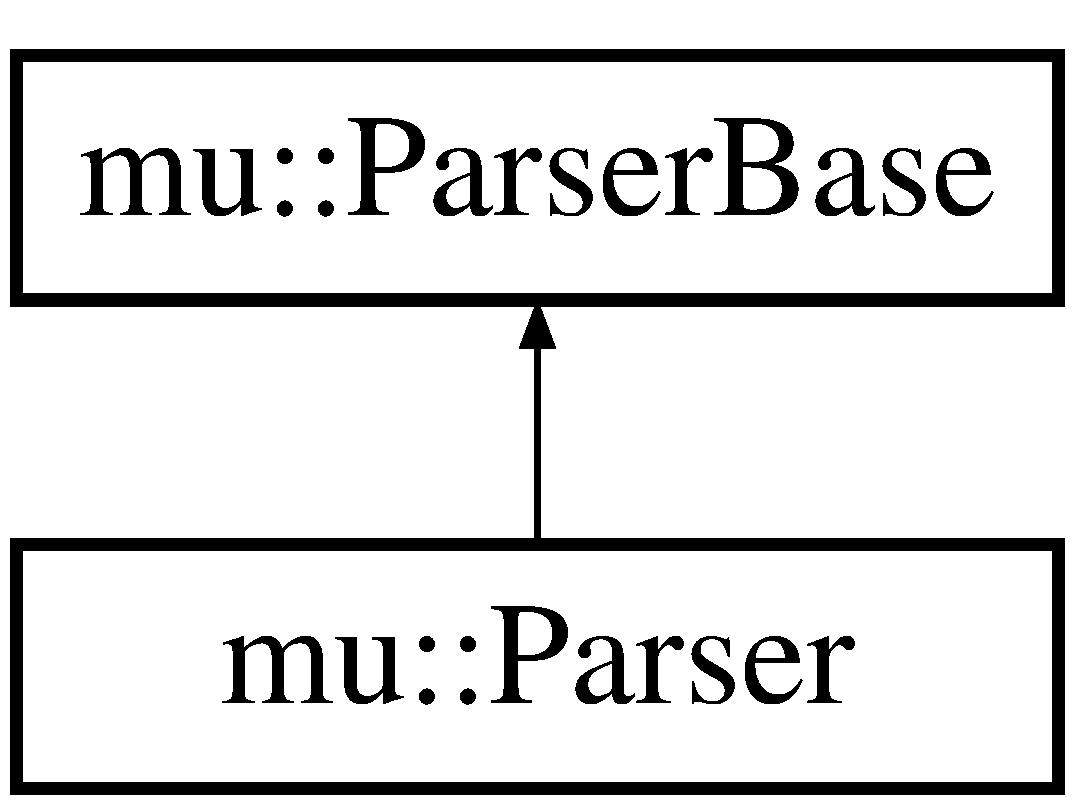
\includegraphics[height=2cm]{classmu_1_1Parser}
\end{center}
\end{figure}


\subsection{Detailed Description}
Mathematical expressions parser. 

Standard implementation of the mathematical expressions parser. Can be used as a reference implementation for subclassing the parser.


\footnotesize  (C) 2004-2008 Ingo Berg\par
 ingo\_\-berg(at)gmx.de 
\normalsize  \subsection*{Public Member Functions}
\begin{CompactItemize}
\item 
{\bf Parser} ()
\begin{CompactList}\small\item\em Constructor. \item\end{CompactList}\item 
virtual void {\bf InitCharSets} ()
\begin{CompactList}\small\item\em Define the character sets. \item\end{CompactList}\item 
virtual void {\bf InitFun} ()
\begin{CompactList}\small\item\em Initialize the default functions. \item\end{CompactList}\item 
virtual void {\bf InitConst} ()
\begin{CompactList}\small\item\em Initialize constants. \item\end{CompactList}\item 
virtual void {\bf InitOprt} ()
\begin{CompactList}\small\item\em Initialize operators. \item\end{CompactList}\item 
void {\bf SetDecSep} ({\bf char\_\-type} cDecSep)
\begin{CompactList}\small\item\em Set the decimal separator. \item\end{CompactList}\item 
void {\bf SetThousandsSep} ({\bf char\_\-type} cThousandsSep)
\begin{CompactList}\small\item\em Sets the thousands operator. \item\end{CompactList}\item 
{\bf value\_\-type} {\bf Diff} ({\bf value\_\-type} $\ast$a\_\-Var, {\bf value\_\-type} a\_\-fPos, {\bf value\_\-type} a\_\-fEpsilon=0.00074) const 
\begin{CompactList}\small\item\em Numerically differentiate with regard to a variable. \item\end{CompactList}\end{CompactItemize}
\subsection*{Classes}
\begin{CompactItemize}
\item 
class \textbf{change\_\-dec\_\-sep}
\begin{CompactList}\small\item\em A facet class used to change decimal and thousands separator. \item\end{CompactList}\end{CompactItemize}


\subsection{Constructor \& Destructor Documentation}
\index{mu::Parser@{mu::Parser}!Parser@{Parser}}
\index{Parser@{Parser}!mu::Parser@{mu::Parser}}
\subsubsection[Parser]{\setlength{\rightskip}{0pt plus 5cm}mu::Parser::Parser ()}\label{classmu_1_1Parser_76747bbf8c232e488e15f846e1b4ed34}


Constructor. 

Call \doxyref{ParserBase}{p.}{classmu_1_1ParserBase} class constructor and trigger Function, Operator and Constant initialization. 

References mu::ParserBase::AddValIdent(), InitCharSets(), InitConst(), InitFun(), and InitOprt().

\subsection{Member Function Documentation}
\index{mu::Parser@{mu::Parser}!InitCharSets@{InitCharSets}}
\index{InitCharSets@{InitCharSets}!mu::Parser@{mu::Parser}}
\subsubsection[InitCharSets]{\setlength{\rightskip}{0pt plus 5cm}void mu::Parser::InitCharSets ()\hspace{0.3cm}{\tt  [virtual]}}\label{classmu_1_1Parser_3279e2cf701ba8c2f850f5826a147f75}


Define the character sets. 

\begin{Desc}
\item[See also:]\doxyref{DefineNameChars}{p.}{classmu_1_1ParserBase_df259477bbaa85e8dd7cb69ef4aa0a7a}, \doxyref{DefineOprtChars}{p.}{classmu_1_1ParserBase_afd21c418397d5412a75e5b2c1d6db58}, \doxyref{DefineInfixOprtChars}{p.}{classmu_1_1ParserBase_c76d0ceb4ee58babc4f1d0a9ca1e4240}\end{Desc}
This function is used for initializing the default character sets that define the characters to be useable in function and variable names and operators. 

Implements {\bf mu::ParserBase} \doxyref{}{p.}{classmu_1_1ParserBase_3f5c53ef3cba6ab939261677dc2d9709}.

References mu::ParserBase::DefineInfixOprtChars(), mu::ParserBase::DefineNameChars(), and mu::ParserBase::DefineOprtChars().

Referenced by Parser().\index{mu::Parser@{mu::Parser}!InitFun@{InitFun}}
\index{InitFun@{InitFun}!mu::Parser@{mu::Parser}}
\subsubsection[InitFun]{\setlength{\rightskip}{0pt plus 5cm}void mu::Parser::InitFun ()\hspace{0.3cm}{\tt  [virtual]}}\label{classmu_1_1Parser_9da582fd5385acfd97ec99a8790f8c6d}


Initialize the default functions. 



Implements {\bf mu::ParserBase} \doxyref{}{p.}{classmu_1_1ParserBase_1f94305e7b7e9abff6d41242dcf188ed}.

Referenced by Parser().\index{mu::Parser@{mu::Parser}!InitConst@{InitConst}}
\index{InitConst@{InitConst}!mu::Parser@{mu::Parser}}
\subsubsection[InitConst]{\setlength{\rightskip}{0pt plus 5cm}void mu::Parser::InitConst ()\hspace{0.3cm}{\tt  [virtual]}}\label{classmu_1_1Parser_efd1da7ba62d20d7276b1e70c8cb6a02}


Initialize constants. 

By default the parser recognizes two constants. Pi (\char`\"{}pi\char`\"{}) and the eulerian number (\char`\"{}\_\-e\char`\"{}). 

Implements {\bf mu::ParserBase} \doxyref{}{p.}{classmu_1_1ParserBase_ad904fb3df8f28659f36d7ce7db4a28c}.

References mu::ParserBase::DefineConst(), PARSER\_\-CONST\_\-E, and PARSER\_\-CONST\_\-PI.

Referenced by Parser().\index{mu::Parser@{mu::Parser}!InitOprt@{InitOprt}}
\index{InitOprt@{InitOprt}!mu::Parser@{mu::Parser}}
\subsubsection[InitOprt]{\setlength{\rightskip}{0pt plus 5cm}void mu::Parser::InitOprt ()\hspace{0.3cm}{\tt  [virtual]}}\label{classmu_1_1Parser_4ed9bdd0565bd57325bc49c12cf73e06}


Initialize operators. 

By default only the unary minus operator is added. 

Implements {\bf mu::ParserBase} \doxyref{}{p.}{classmu_1_1ParserBase_4df16813c9002ff08c96929ba8f0d32b}.

References mu::ParserBase::DefineInfixOprt().

Referenced by Parser().\index{mu::Parser@{mu::Parser}!SetDecSep@{SetDecSep}}
\index{SetDecSep@{SetDecSep}!mu::Parser@{mu::Parser}}
\subsubsection[SetDecSep]{\setlength{\rightskip}{0pt plus 5cm}void mu::Parser::SetDecSep ({\bf char\_\-type} {\em cDecSep})}\label{classmu_1_1Parser_8f7441d77774d6bbb5b6a260985b5e8e}


Set the decimal separator. 

\begin{Desc}
\item[Parameters:]
\begin{description}
\item[{\em cDecSep}]Decimal separator as a character value. \end{description}
\end{Desc}
\begin{Desc}
\item[See also:]\doxyref{SetThousandsSep}{p.}{classmu_1_1Parser_a844b84c174a91afa6e339102f362b81}\end{Desc}
By default muparser uses the \char`\"{}C\char`\"{} locale. The decimal separator of this locale is overwritten by the one provided here. \index{mu::Parser@{mu::Parser}!SetThousandsSep@{SetThousandsSep}}
\index{SetThousandsSep@{SetThousandsSep}!mu::Parser@{mu::Parser}}
\subsubsection[SetThousandsSep]{\setlength{\rightskip}{0pt plus 5cm}void mu::Parser::SetThousandsSep ({\bf char\_\-type} {\em cThousandsSep})}\label{classmu_1_1Parser_a844b84c174a91afa6e339102f362b81}


Sets the thousands operator. 

\begin{Desc}
\item[Parameters:]
\begin{description}
\item[{\em cThousandsSep}]The thousands separator as a character \end{description}
\end{Desc}
\begin{Desc}
\item[See also:]\doxyref{SetDecSep}{p.}{classmu_1_1Parser_8f7441d77774d6bbb5b6a260985b5e8e}\end{Desc}
By default muparser uses the \char`\"{}C\char`\"{} locale. The thousands separator of this locale is overwritten by the one provided here. \index{mu::Parser@{mu::Parser}!Diff@{Diff}}
\index{Diff@{Diff}!mu::Parser@{mu::Parser}}
\subsubsection[Diff]{\setlength{\rightskip}{0pt plus 5cm}{\bf value\_\-type} mu::Parser::Diff ({\bf value\_\-type} $\ast$ {\em a\_\-Var}, \/  {\bf value\_\-type} {\em a\_\-fPos}, \/  {\bf value\_\-type} {\em a\_\-fEpsilon} = {\tt 0.00074}) const}\label{classmu_1_1Parser_cc00dfac0da35d3b844f08a62984b197}


Numerically differentiate with regard to a variable. 

\begin{Desc}
\item[Parameters:]
\begin{description}
\item[\mbox{$\leftarrow$} {\em a\_\-Var}]Pointer to the differentiation variable. \item[\mbox{$\leftarrow$} {\em a\_\-fPos}]Position at which the differentiation should take place. \item[\mbox{$\leftarrow$} {\em a\_\-fEpsilon}]Epsilon used for the numerical differentiation.\end{description}
\end{Desc}
Numerical differentiation uses a 5 point operator yielding a 4th order formula. The default value for epsilon is 0.00074 which is numerical\_\-limits$<$double$>$::epsilon() $^\wedge$ (1/5) as suggested in the muparser forum:

{\tt http://sourceforge.net/forum/forum.php?thread\_\-id=1994611\&forum\_\-id=462843} 

References mu::ParserBase::Eval().

The documentation for this class was generated from the following files:\begin{CompactItemize}
\item 
{\bf muParser.h}\item 
{\bf muParser.cpp}\end{CompactItemize}

\section{mu::ParserBase Class Reference}
\label{classmu_1_1ParserBase}\index{mu::ParserBase@{mu::ParserBase}}
{\tt \#include $<$muParserBase.h$>$}

Inheritance diagram for mu::ParserBase::\begin{figure}[H]
\begin{center}
\leavevmode
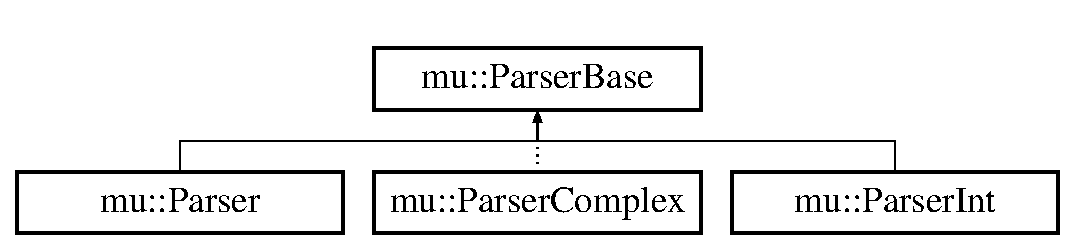
\includegraphics[height=2cm]{classmu_1_1ParserBase}
\end{center}
\end{figure}


\subsection{Detailed Description}
Mathematical expressions parser (base parser engine). 

Version 1.30 (20080413)

This is the implementation of a bytecode based mathematical expressions parser. The formula will be parsed from string and converted into a bytecode. Future calculations will be done with the bytecode instead the formula string resulting in a significant performance increase. Complementary to a set of internally implemented functions the parser is able to handle user defined functions and variables.

\begin{Desc}
\item[Author:](C) 2004-2008 Ingo Berg \end{Desc}
\subsection*{Public Types}
\begin{CompactItemize}
\item 
typedef {\bf ParserError} {\bf exception\_\-type}
\begin{CompactList}\small\item\em Type of the error class. \item\end{CompactList}\end{CompactItemize}
\subsection*{Public Member Functions}
\begin{CompactItemize}
\item 
{\bf ParserBase} ()
\begin{CompactList}\small\item\em Constructor. \item\end{CompactList}\item 
{\bf ParserBase} (const {\bf ParserBase} \&a\_\-Parser)
\item 
{\bf ParserBase} \& {\bf operator=} (const {\bf ParserBase} \&a\_\-Parser)
\begin{CompactList}\small\item\em Assignement operator. \item\end{CompactList}\item 
virtual {\bf $\sim$ParserBase} ()
\item 
{\bf value\_\-type} {\bf Eval} () const 
\begin{CompactList}\small\item\em Calculate the result. \item\end{CompactList}\item 
void {\bf SetExpr} (const {\bf string\_\-type} \&a\_\-sExpr)
\begin{CompactList}\small\item\em Set the formula. \item\end{CompactList}\item 
void {\bf SetVarFactory} ({\bf facfun\_\-type} a\_\-pFactory, void $\ast$pUserData=NULL)
\item 
void {\bf EnableOptimizer} (bool a\_\-bIsOn=true)
\begin{CompactList}\small\item\em Enable or disable the formula optimization feature. \item\end{CompactList}\item 
void {\bf EnableByteCode} (bool a\_\-bIsOn=true)
\begin{CompactList}\small\item\em Enable or disable parsing from Bytecode. \item\end{CompactList}\item 
void {\bf EnableBuiltInOprt} (bool a\_\-bIsOn=true)
\begin{CompactList}\small\item\em Enable or disable the built in binary operators. \item\end{CompactList}\item 
bool {\bf HasBuiltInOprt} () const 
\begin{CompactList}\small\item\em Query status of built in variables. \item\end{CompactList}\item 
void {\bf AddValIdent} ({\bf identfun\_\-type} a\_\-pCallback)
\item 
void {\bf DefineOprt} (const {\bf string\_\-type} \&a\_\-strName, {\bf fun\_\-type2} a\_\-pFun, unsigned a\_\-iPri=0, bool a\_\-bAllowOpt=false)
\begin{CompactList}\small\item\em Define a binary operator. \item\end{CompactList}\item 
void {\bf DefineConst} (const {\bf string\_\-type} \&a\_\-sName, {\bf value\_\-type} a\_\-fVal)
\begin{CompactList}\small\item\em Add a user defined constant. \item\end{CompactList}\item 
void {\bf DefineStrConst} (const {\bf string\_\-type} \&a\_\-sName, const {\bf string\_\-type} \&a\_\-strVal)
\begin{CompactList}\small\item\em Define a new string constant. \item\end{CompactList}\item 
void {\bf DefineVar} (const {\bf string\_\-type} \&a\_\-sName, {\bf value\_\-type} $\ast$a\_\-fVar)
\begin{CompactList}\small\item\em Add a user defined variable. \item\end{CompactList}\item 
void {\bf DefinePostfixOprt} (const {\bf string\_\-type} \&a\_\-strFun, {\bf fun\_\-type1} a\_\-pOprt, bool a\_\-bAllowOpt=true)
\begin{CompactList}\small\item\em Add a user defined operator. \item\end{CompactList}\item 
void {\bf DefineInfixOprt} (const {\bf string\_\-type} \&a\_\-strName, {\bf fun\_\-type1} a\_\-pOprt, int a\_\-iPrec=prINFIX, bool a\_\-bAllowOpt=true)
\begin{CompactList}\small\item\em Add a user defined operator. \item\end{CompactList}\item 
void {\bf ClearVar} ()
\begin{CompactList}\small\item\em Clear all user defined variables. \item\end{CompactList}\item 
void {\bf ClearFun} ()
\begin{CompactList}\small\item\em Clear all functions. \item\end{CompactList}\item 
void {\bf ClearConst} ()
\begin{CompactList}\small\item\em Clear all user defined constants. \item\end{CompactList}\item 
void {\bf ClearInfixOprt} ()
\begin{CompactList}\small\item\em Clear the user defined Prefix operators. \item\end{CompactList}\item 
void {\bf ClearPostfixOprt} ()
\begin{CompactList}\small\item\em Clear all user defined postfix operators. \item\end{CompactList}\item 
void {\bf ClearOprt} ()
\begin{CompactList}\small\item\em Clear all user defined binary operators. \item\end{CompactList}\item 
void {\bf RemoveVar} (const {\bf string\_\-type} \&a\_\-strVarName)
\begin{CompactList}\small\item\em Remove a variable from internal storage. \item\end{CompactList}\item 
const {\bf varmap\_\-type} \& {\bf GetUsedVar} () const 
\begin{CompactList}\small\item\em Return a map containing the used variables only. \item\end{CompactList}\item 
const {\bf varmap\_\-type} \& {\bf GetVar} () const 
\begin{CompactList}\small\item\em Return a map containing the used variables only. \item\end{CompactList}\item 
const {\bf valmap\_\-type} \& {\bf GetConst} () const 
\begin{CompactList}\small\item\em Return a map containing all parser constants. \item\end{CompactList}\item 
const {\bf string\_\-type} \& {\bf GetExpr} () const 
\begin{CompactList}\small\item\em Retrieve the formula. \item\end{CompactList}\item 
const {\bf funmap\_\-type} \& {\bf GetFunDef} () const 
\begin{CompactList}\small\item\em Return prototypes of all parser functions. \item\end{CompactList}\item 
const {\bf char\_\-type} $\ast$$\ast$ {\bf GetOprtDef} () const 
\begin{CompactList}\small\item\em Get the default symbols used for the built in operators. \item\end{CompactList}\item 
void {\bf DefineNameChars} (const {\bf char\_\-type} $\ast$a\_\-szCharset)
\begin{CompactList}\small\item\em Define the set of valid characters to be used in names of functions, variables, constants. \item\end{CompactList}\item 
void {\bf DefineOprtChars} (const {\bf char\_\-type} $\ast$a\_\-szCharset)
\begin{CompactList}\small\item\em Define the set of valid characters to be used in names of binary operators and postfix operators. \item\end{CompactList}\item 
void {\bf DefineInfixOprtChars} (const {\bf char\_\-type} $\ast$a\_\-szCharset)
\begin{CompactList}\small\item\em Define the set of valid characters to be used in names of infix operators. \item\end{CompactList}\item 
const {\bf char\_\-type} $\ast$ {\bf ValidNameChars} () const 
\begin{CompactList}\small\item\em Virtual function that defines the characters allowed in name identifiers. \item\end{CompactList}\item 
const {\bf char\_\-type} $\ast$ {\bf ValidOprtChars} () const 
\begin{CompactList}\small\item\em Virtual function that defines the characters allowed in operator definitions. \item\end{CompactList}\item 
const {\bf char\_\-type} $\ast$ {\bf ValidInfixOprtChars} () const 
\begin{CompactList}\small\item\em Virtual function that defines the characters allowed in infix operator definitions. \item\end{CompactList}\item 
void {\bf SetArgSep} ({\bf char\_\-type} cArgSep)
\begin{CompactList}\small\item\em Set argument separator. \item\end{CompactList}\item 
{\bf char\_\-type} {\bf GetArgSep} () const 
\begin{CompactList}\small\item\em Get the argument separator character. \item\end{CompactList}\item 
void {\bf Error} ({\bf EErrorCodes} a\_\-iErrc, int a\_\-iPos=(int) mu::string\_\-type::npos, const {\bf string\_\-type} \&a\_\-strTok={\bf string\_\-type}()) const 
\begin{CompactList}\small\item\em Create an error containing the parse error position. \item\end{CompactList}\end{CompactItemize}
\subsection*{Protected Member Functions}
\begin{CompactItemize}
\item 
void {\bf Init} ()
\begin{CompactList}\small\item\em Initialize user defined functions. \item\end{CompactList}\item 
virtual void {\bf InitCharSets} ()=0
\item 
virtual void {\bf InitFun} ()=0
\item 
virtual void {\bf InitConst} ()=0
\item 
virtual void {\bf InitOprt} ()=0
\end{CompactItemize}
\subsection*{Static Protected Attributes}
\begin{CompactItemize}
\item 
static {\bf char\_\-type} $\ast$ {\bf c\_\-DefaultOprt} [$\,$]
\begin{CompactList}\small\item\em Identifiers for built in binary operators. \item\end{CompactList}\end{CompactItemize}
\subsection*{Friends}
\begin{CompactItemize}
\item 
class {\bf ParserTokenReader}
\end{CompactItemize}


\subsection{Member Typedef Documentation}
\index{mu::ParserBase@{mu::ParserBase}!exception\_\-type@{exception\_\-type}}
\index{exception\_\-type@{exception\_\-type}!mu::ParserBase@{mu::ParserBase}}
\subsubsection[exception\_\-type]{\setlength{\rightskip}{0pt plus 5cm}typedef {\bf ParserError} {\bf mu::ParserBase::exception\_\-type}}\label{classmu_1_1ParserBase_b385f37be00cee7d8a68c3c41f6a5b64}


Type of the error class. 

Included for backwards compatibility. 

\subsection{Constructor \& Destructor Documentation}
\index{mu::ParserBase@{mu::ParserBase}!ParserBase@{ParserBase}}
\index{ParserBase@{ParserBase}!mu::ParserBase@{mu::ParserBase}}
\subsubsection[ParserBase]{\setlength{\rightskip}{0pt plus 5cm}mu::ParserBase::ParserBase ()}\label{classmu_1_1ParserBase_41d13be909945b892777ee6773fa1f69}


Constructor. 

\begin{Desc}
\item[Parameters:]
\begin{description}
\item[{\em a\_\-szFormula}]the formula to interpret. \end{description}
\end{Desc}
\begin{Desc}
\item[Exceptions:]
\begin{description}
\item[{\em ParserException}]if a\_\-szFormula is null. \end{description}
\end{Desc}
\index{mu::ParserBase@{mu::ParserBase}!ParserBase@{ParserBase}}
\index{ParserBase@{ParserBase}!mu::ParserBase@{mu::ParserBase}}
\subsubsection[ParserBase]{\setlength{\rightskip}{0pt plus 5cm}mu::ParserBase::ParserBase (const {\bf ParserBase} \& {\em a\_\-Parser})}\label{classmu_1_1ParserBase_88d9367e1a71bc07fe587633060223a0}


\index{mu::ParserBase@{mu::ParserBase}!$\sim$ParserBase@{$\sim$ParserBase}}
\index{$\sim$ParserBase@{$\sim$ParserBase}!mu::ParserBase@{mu::ParserBase}}
\subsubsection[$\sim$ParserBase]{\setlength{\rightskip}{0pt plus 5cm}mu::ParserBase::$\sim$ParserBase ()\hspace{0.3cm}{\tt  [virtual]}}\label{classmu_1_1ParserBase_94ec173a26a5ffc96325287830a44caa}




\subsection{Member Function Documentation}
\index{mu::ParserBase@{mu::ParserBase}!operator=@{operator=}}
\index{operator=@{operator=}!mu::ParserBase@{mu::ParserBase}}
\subsubsection[operator=]{\setlength{\rightskip}{0pt plus 5cm}{\bf ParserBase} \& mu::ParserBase::operator= (const {\bf ParserBase} \& {\em a\_\-Parser})}\label{classmu_1_1ParserBase_ca7cf1ea7f82dfb3066ada8427295a4c}


Assignement operator. 

Implemented by calling Assign(a\_\-Parser). Self assignement is suppressed. \begin{Desc}
\item[Parameters:]
\begin{description}
\item[{\em a\_\-Parser}]Object to copy to this. \end{description}
\end{Desc}
\begin{Desc}
\item[Returns:]$\ast$this \end{Desc}
\begin{Desc}
\item[Exceptions:]
\begin{description}
\item[{\em nothrow}]\end{description}
\end{Desc}
\index{mu::ParserBase@{mu::ParserBase}!Eval@{Eval}}
\index{Eval@{Eval}!mu::ParserBase@{mu::ParserBase}}
\subsubsection[Eval]{\setlength{\rightskip}{0pt plus 5cm}{\bf value\_\-type} mu::ParserBase::Eval () const\hspace{0.3cm}{\tt  [inline]}}\label{classmu_1_1ParserBase_9f91f5d3c0acd2e30225eb97867dc651}


Calculate the result. 

A note on const correctness: I consider it important that Calc is a const function. Due to caching operations Calc changes only the state of internal variables with one exception m\_\-UsedVar this is reset during string parsing and accessible from the outside. Instead of making Calc non const GetUsedVar is non const because it explicitely calls \doxyref{Eval()}{p.}{classmu_1_1ParserBase_9f91f5d3c0acd2e30225eb97867dc651} forcing this update.

\begin{Desc}
\item[Precondition:]A formula must be set. 

Variables must have been set (if needed)\end{Desc}
\begin{Desc}
\item[See also:]m\_\-pParseFormula \end{Desc}
\begin{Desc}
\item[Returns:]The evaluation result \end{Desc}
\begin{Desc}
\item[Exceptions:]
\begin{description}
\item[{\em ParseException}]if no Formula is set or in case of any other error related to the formula. \end{description}
\end{Desc}


Referenced by mu::Parser::Diff(), and mu::ParserComplex::Eval().\index{mu::ParserBase@{mu::ParserBase}!SetExpr@{SetExpr}}
\index{SetExpr@{SetExpr}!mu::ParserBase@{mu::ParserBase}}
\subsubsection[SetExpr]{\setlength{\rightskip}{0pt plus 5cm}void mu::ParserBase::SetExpr (const {\bf string\_\-type} \& {\em a\_\-sExpr})}\label{classmu_1_1ParserBase_ed9d02dd04f8e163102f9a8e082c4b26}


Set the formula. 

\begin{Desc}
\item[Parameters:]
\begin{description}
\item[{\em a\_\-strFormula}]Formula as string\_\-type \end{description}
\end{Desc}
\begin{Desc}
\item[Exceptions:]
\begin{description}
\item[{\em ParserException}]in case of syntax errors.\end{description}
\end{Desc}
Triggers first time calculation thus the creation of the bytecode and scanning of used variables. 

References mu::ecLOCALE, and Error().\index{mu::ParserBase@{mu::ParserBase}!SetVarFactory@{SetVarFactory}}
\index{SetVarFactory@{SetVarFactory}!mu::ParserBase@{mu::ParserBase}}
\subsubsection[SetVarFactory]{\setlength{\rightskip}{0pt plus 5cm}void mu::ParserBase::SetVarFactory ({\bf facfun\_\-type} {\em a\_\-pFactory}, \/  void $\ast$ {\em pUserData} = {\tt NULL})}\label{classmu_1_1ParserBase_713d8ddf5371c346942d22fdac5adda7}


\index{mu::ParserBase@{mu::ParserBase}!EnableOptimizer@{EnableOptimizer}}
\index{EnableOptimizer@{EnableOptimizer}!mu::ParserBase@{mu::ParserBase}}
\subsubsection[EnableOptimizer]{\setlength{\rightskip}{0pt plus 5cm}void mu::ParserBase::EnableOptimizer (bool {\em a\_\-bIsOn} = {\tt true})}\label{classmu_1_1ParserBase_43221e10afd17efe8d32898707763cb4}


Enable or disable the formula optimization feature. 

\begin{Desc}
\item[Postcondition:]Resets the parser to string parser mode. \end{Desc}
\begin{Desc}
\item[Exceptions:]
\begin{description}
\item[{\em nothrow}]\end{description}
\end{Desc}
\index{mu::ParserBase@{mu::ParserBase}!EnableByteCode@{EnableByteCode}}
\index{EnableByteCode@{EnableByteCode}!mu::ParserBase@{mu::ParserBase}}
\subsubsection[EnableByteCode]{\setlength{\rightskip}{0pt plus 5cm}void mu::ParserBase::EnableByteCode (bool {\em a\_\-bIsOn} = {\tt true})}\label{classmu_1_1ParserBase_61f4495b8b1e89924f01fe392e2e521f}


Enable or disable parsing from Bytecode. 

\begin{Desc}
\item[Attention:]There is no reason to disable bytecode. It will drastically decrease parsing speed. \end{Desc}
\index{mu::ParserBase@{mu::ParserBase}!EnableBuiltInOprt@{EnableBuiltInOprt}}
\index{EnableBuiltInOprt@{EnableBuiltInOprt}!mu::ParserBase@{mu::ParserBase}}
\subsubsection[EnableBuiltInOprt]{\setlength{\rightskip}{0pt plus 5cm}void mu::ParserBase::EnableBuiltInOprt (bool {\em a\_\-bIsOn} = {\tt true})}\label{classmu_1_1ParserBase_df5cb2ffd21f51fac2633a4976fe1e2d}


Enable or disable the built in binary operators. 

\begin{Desc}
\item[Exceptions:]
\begin{description}
\item[{\em nothrow}]\end{description}
\end{Desc}
\begin{Desc}
\item[See also:]m\_\-bBuiltInOp, ReInit()\end{Desc}
If you disable the built in binary operators there will be no binary operators defined. Thus you must add them manually one by one. It is not possible to disable built in operators selectively. This function will Reinitialize the parser by calling ReInit(). 

Referenced by mu::ParserInt::InitOprt().\index{mu::ParserBase@{mu::ParserBase}!HasBuiltInOprt@{HasBuiltInOprt}}
\index{HasBuiltInOprt@{HasBuiltInOprt}!mu::ParserBase@{mu::ParserBase}}
\subsubsection[HasBuiltInOprt]{\setlength{\rightskip}{0pt plus 5cm}bool mu::ParserBase::HasBuiltInOprt () const}\label{classmu_1_1ParserBase_b1f44f5270153cefe9595f06581ffd29}


Query status of built in variables. 

\begin{Desc}
\item[Returns:]m\_\-bBuiltInOp; true if built in operators are enabled. \end{Desc}
\begin{Desc}
\item[Exceptions:]
\begin{description}
\item[{\em nothrow}]\end{description}
\end{Desc}
\index{mu::ParserBase@{mu::ParserBase}!AddValIdent@{AddValIdent}}
\index{AddValIdent@{AddValIdent}!mu::ParserBase@{mu::ParserBase}}
\subsubsection[AddValIdent]{\setlength{\rightskip}{0pt plus 5cm}void mu::ParserBase::AddValIdent ({\bf identfun\_\-type} {\em a\_\-pCallback})}\label{classmu_1_1ParserBase_0b49dbe051415f9d2a9d5564c38609e3}




Referenced by mu::Parser::Parser(), mu::ParserComplex::ParserComplex(), and mu::ParserInt::ParserInt().\index{mu::ParserBase@{mu::ParserBase}!DefineOprt@{DefineOprt}}
\index{DefineOprt@{DefineOprt}!mu::ParserBase@{mu::ParserBase}}
\subsubsection[DefineOprt]{\setlength{\rightskip}{0pt plus 5cm}void mu::ParserBase::DefineOprt (const {\bf string\_\-type} \& {\em a\_\-sName}, \/  {\bf fun\_\-type2} {\em a\_\-pFun}, \/  unsigned {\em a\_\-iPrec} = {\tt 0}, \/  bool {\em a\_\-bAllowOpt} = {\tt false})}\label{classmu_1_1ParserBase_aabe9ed5581edf62ad51d02bb17c4f54}


Define a binary operator. 

\begin{Desc}
\item[Parameters:]
\begin{description}
\item[\mbox{$\leftarrow$} {\em a\_\-pFun}]Pointer to the callback function. \item[\mbox{$\leftarrow$} {\em a\_\-iPrec}]Precedence of the operator. \item[\mbox{$\leftarrow$} {\em a\_\-bAllowOpt}]If this is true the operator may be optimized away. \end{description}
\end{Desc}


References c\_\-DefaultOprt, mu::cmARG\_\-SEP, mu::cmOPRT\_\-BIN, mu::ecBUILTIN\_\-OVERLOAD, Error(), and ValidOprtChars().

Referenced by mu::ParserInt::InitOprt().\index{mu::ParserBase@{mu::ParserBase}!DefineConst@{DefineConst}}
\index{DefineConst@{DefineConst}!mu::ParserBase@{mu::ParserBase}}
\subsubsection[DefineConst]{\setlength{\rightskip}{0pt plus 5cm}void mu::ParserBase::DefineConst (const {\bf string\_\-type} \& {\em a\_\-sName}, \/  {\bf value\_\-type} {\em a\_\-fVal})}\label{classmu_1_1ParserBase_8cbb0a5e193daeea647d80dc89f34c65}


Add a user defined constant. 

\begin{Desc}
\item[Parameters:]
\begin{description}
\item[\mbox{$\leftarrow$} {\em a\_\-sName}]The name of the constant. \item[\mbox{$\leftarrow$} {\em a\_\-fVal}]the value of the constant. \end{description}
\end{Desc}
\begin{Desc}
\item[Postcondition:]Will reset the \doxyref{Parser}{p.}{classmu_1_1Parser} to string parsing mode. \end{Desc}
\begin{Desc}
\item[Exceptions:]
\begin{description}
\item[{\em ParserException}]in case the name contains invalid signs. \end{description}
\end{Desc}


References ValidNameChars().

Referenced by mu::Parser::InitConst().\index{mu::ParserBase@{mu::ParserBase}!DefineStrConst@{DefineStrConst}}
\index{DefineStrConst@{DefineStrConst}!mu::ParserBase@{mu::ParserBase}}
\subsubsection[DefineStrConst]{\setlength{\rightskip}{0pt plus 5cm}void mu::ParserBase::DefineStrConst (const {\bf string\_\-type} \& {\em a\_\-strName}, \/  const {\bf string\_\-type} \& {\em a\_\-strVal})}\label{classmu_1_1ParserBase_64bc1de3b6db42140fe6f4860c30e40a}


Define a new string constant. 

\begin{Desc}
\item[Parameters:]
\begin{description}
\item[\mbox{$\leftarrow$} {\em a\_\-strName}]The name of the constant. \item[\mbox{$\leftarrow$} {\em a\_\-strVal}]the value of the constant. \end{description}
\end{Desc}


References mu::ecNAME\_\-CONFLICT, Error(), and ValidNameChars().\index{mu::ParserBase@{mu::ParserBase}!DefineVar@{DefineVar}}
\index{DefineVar@{DefineVar}!mu::ParserBase@{mu::ParserBase}}
\subsubsection[DefineVar]{\setlength{\rightskip}{0pt plus 5cm}void mu::ParserBase::DefineVar (const {\bf string\_\-type} \& {\em a\_\-sName}, \/  {\bf value\_\-type} $\ast$ {\em a\_\-pVar})}\label{classmu_1_1ParserBase_8350970819c77352af8d79ce3110393e}


Add a user defined variable. 

\begin{Desc}
\item[Parameters:]
\begin{description}
\item[\mbox{$\leftarrow$} {\em a\_\-sName}]the variable name \item[\mbox{$\leftarrow$} {\em a\_\-pVar}]A pointer to the variable vaule. \end{description}
\end{Desc}
\begin{Desc}
\item[Postcondition:]Will reset the \doxyref{Parser}{p.}{classmu_1_1Parser} to string parsing mode. \end{Desc}
\begin{Desc}
\item[Precondition:][assert] a\_\-fVar!=0 \end{Desc}
\begin{Desc}
\item[Exceptions:]
\begin{description}
\item[{\em ParserException}]in case the name contains invalid signs. \end{description}
\end{Desc}


References mu::ecINVALID\_\-VAR\_\-PTR, mu::ecNAME\_\-CONFLICT, Error(), and ValidNameChars().\index{mu::ParserBase@{mu::ParserBase}!DefinePostfixOprt@{DefinePostfixOprt}}
\index{DefinePostfixOprt@{DefinePostfixOprt}!mu::ParserBase@{mu::ParserBase}}
\subsubsection[DefinePostfixOprt]{\setlength{\rightskip}{0pt plus 5cm}void mu::ParserBase::DefinePostfixOprt (const {\bf string\_\-type} \& {\em a\_\-sName}, \/  {\bf fun\_\-type1} {\em a\_\-pFun}, \/  bool {\em a\_\-bAllowOpt} = {\tt true})}\label{classmu_1_1ParserBase_e9fb4d2348213a0e42dc07a4589ac654}


Add a user defined operator. 

\begin{Desc}
\item[Postcondition:]Will reset the \doxyref{Parser}{p.}{classmu_1_1Parser} to string parsing mode. \end{Desc}


References mu::cmOPRT\_\-POSTFIX, mu::prPOSTFIX, and ValidOprtChars().\index{mu::ParserBase@{mu::ParserBase}!DefineInfixOprt@{DefineInfixOprt}}
\index{DefineInfixOprt@{DefineInfixOprt}!mu::ParserBase@{mu::ParserBase}}
\subsubsection[DefineInfixOprt]{\setlength{\rightskip}{0pt plus 5cm}void mu::ParserBase::DefineInfixOprt (const {\bf string\_\-type} \& {\em a\_\-sName}, \/  {\bf fun\_\-type1} {\em a\_\-pFun}, \/  int {\em a\_\-iPrec} = {\tt prINFIX}, \/  bool {\em a\_\-bAllowOpt} = {\tt true})}\label{classmu_1_1ParserBase_5e26f06efc7564a85a5f5ab682ba5a23}


Add a user defined operator. 

\begin{Desc}
\item[Postcondition:]Will reset the \doxyref{Parser}{p.}{classmu_1_1Parser} to string parsing mode. \end{Desc}
\begin{Desc}
\item[Parameters:]
\begin{description}
\item[\mbox{$\leftarrow$} {\em a\_\-sName}]operator Identifier \item[\mbox{$\leftarrow$} {\em a\_\-pFun}]Operator callback function \item[\mbox{$\leftarrow$} {\em a\_\-iPrec}]Operator Precedence (default=prSIGN) \item[\mbox{$\leftarrow$} {\em a\_\-bAllowOpt}]True if operator is volatile (default=false) \end{description}
\end{Desc}
\begin{Desc}
\item[See also:]\doxyref{EPrec}{p.}{namespacemu_bcc2208f2cb6f0f3ffe36adec0a07aea} \end{Desc}


References mu::cmOPRT\_\-INFIX, and ValidOprtChars().

Referenced by mu::ParserInt::InitOprt(), and mu::Parser::InitOprt().\index{mu::ParserBase@{mu::ParserBase}!ClearVar@{ClearVar}}
\index{ClearVar@{ClearVar}!mu::ParserBase@{mu::ParserBase}}
\subsubsection[ClearVar]{\setlength{\rightskip}{0pt plus 5cm}void mu::ParserBase::ClearVar ()}\label{classmu_1_1ParserBase_dd23e405d36de71de6b386bc0eb4b57c}


Clear all user defined variables. 

\begin{Desc}
\item[Exceptions:]
\begin{description}
\item[{\em nothrow}]Resets the parser to string parsing mode by calling ReInit. \end{description}
\end{Desc}
\index{mu::ParserBase@{mu::ParserBase}!ClearFun@{ClearFun}}
\index{ClearFun@{ClearFun}!mu::ParserBase@{mu::ParserBase}}
\subsubsection[ClearFun]{\setlength{\rightskip}{0pt plus 5cm}void mu::ParserBase::ClearFun ()}\label{classmu_1_1ParserBase_bc296c44f8a9522b2cf12a9ad36071b2}


Clear all functions. 

\begin{Desc}
\item[Postcondition:]Resets the parser to string parsing mode. \end{Desc}
\begin{Desc}
\item[Exceptions:]
\begin{description}
\item[{\em nothrow}]\end{description}
\end{Desc}
\index{mu::ParserBase@{mu::ParserBase}!ClearConst@{ClearConst}}
\index{ClearConst@{ClearConst}!mu::ParserBase@{mu::ParserBase}}
\subsubsection[ClearConst]{\setlength{\rightskip}{0pt plus 5cm}void mu::ParserBase::ClearConst ()}\label{classmu_1_1ParserBase_dbc445632a056820ff722ca18c1331e9}


Clear all user defined constants. 

Both numeric and string constants will be removed from the internal storage. \begin{Desc}
\item[Postcondition:]Resets the parser to string parsing mode. \end{Desc}
\begin{Desc}
\item[Exceptions:]
\begin{description}
\item[{\em nothrow}]\end{description}
\end{Desc}
\index{mu::ParserBase@{mu::ParserBase}!ClearInfixOprt@{ClearInfixOprt}}
\index{ClearInfixOprt@{ClearInfixOprt}!mu::ParserBase@{mu::ParserBase}}
\subsubsection[ClearInfixOprt]{\setlength{\rightskip}{0pt plus 5cm}void mu::ParserBase::ClearInfixOprt ()}\label{classmu_1_1ParserBase_7485eccf3281c879dad059966e3cbe22}


Clear the user defined Prefix operators. 

\begin{Desc}
\item[Postcondition:]Resets the parser to string parser mode. \end{Desc}
\begin{Desc}
\item[Exceptions:]
\begin{description}
\item[{\em nothrow}]\end{description}
\end{Desc}
\index{mu::ParserBase@{mu::ParserBase}!ClearPostfixOprt@{ClearPostfixOprt}}
\index{ClearPostfixOprt@{ClearPostfixOprt}!mu::ParserBase@{mu::ParserBase}}
\subsubsection[ClearPostfixOprt]{\setlength{\rightskip}{0pt plus 5cm}void mu::ParserBase::ClearPostfixOprt ()}\label{classmu_1_1ParserBase_b8a8356532f0047d8a33a46bc77f4bc5}


Clear all user defined postfix operators. 

\begin{Desc}
\item[Postcondition:]Resets the parser to string parsing mode. \end{Desc}
\begin{Desc}
\item[Exceptions:]
\begin{description}
\item[{\em nothrow}]\end{description}
\end{Desc}
\index{mu::ParserBase@{mu::ParserBase}!ClearOprt@{ClearOprt}}
\index{ClearOprt@{ClearOprt}!mu::ParserBase@{mu::ParserBase}}
\subsubsection[ClearOprt]{\setlength{\rightskip}{0pt plus 5cm}void mu::ParserBase::ClearOprt ()}\label{classmu_1_1ParserBase_a5fd05a7bb2b8bc9f9745c5377c0ebf3}


Clear all user defined binary operators. 

\begin{Desc}
\item[Postcondition:]Resets the parser to string parsing mode. \end{Desc}
\begin{Desc}
\item[Exceptions:]
\begin{description}
\item[{\em nothrow}]\end{description}
\end{Desc}
\index{mu::ParserBase@{mu::ParserBase}!RemoveVar@{RemoveVar}}
\index{RemoveVar@{RemoveVar}!mu::ParserBase@{mu::ParserBase}}
\subsubsection[RemoveVar]{\setlength{\rightskip}{0pt plus 5cm}void mu::ParserBase::RemoveVar (const {\bf string\_\-type} \& {\em a\_\-strVarName})}\label{classmu_1_1ParserBase_8e5a54620200dfbd42ec084c29249d94}


Remove a variable from internal storage. 

\begin{Desc}
\item[Exceptions:]
\begin{description}
\item[{\em nothrow}]Removes a variable if it exists. If the Variable does not exist nothing will be done. \end{description}
\end{Desc}
\index{mu::ParserBase@{mu::ParserBase}!GetUsedVar@{GetUsedVar}}
\index{GetUsedVar@{GetUsedVar}!mu::ParserBase@{mu::ParserBase}}
\subsubsection[GetUsedVar]{\setlength{\rightskip}{0pt plus 5cm}const {\bf varmap\_\-type} \& mu::ParserBase::GetUsedVar () const}\label{classmu_1_1ParserBase_42cd9be355fea027e5c11acaf1c40767}


Return a map containing the used variables only. 

\index{mu::ParserBase@{mu::ParserBase}!GetVar@{GetVar}}
\index{GetVar@{GetVar}!mu::ParserBase@{mu::ParserBase}}
\subsubsection[GetVar]{\setlength{\rightskip}{0pt plus 5cm}const {\bf varmap\_\-type} \& mu::ParserBase::GetVar () const}\label{classmu_1_1ParserBase_aad6f7b4889b843111f18510f4f5253b}


Return a map containing the used variables only. 

\index{mu::ParserBase@{mu::ParserBase}!GetConst@{GetConst}}
\index{GetConst@{GetConst}!mu::ParserBase@{mu::ParserBase}}
\subsubsection[GetConst]{\setlength{\rightskip}{0pt plus 5cm}const {\bf valmap\_\-type} \& mu::ParserBase::GetConst () const}\label{classmu_1_1ParserBase_0175999f0834125322a615f0b2926be6}


Return a map containing all parser constants. 

\index{mu::ParserBase@{mu::ParserBase}!GetExpr@{GetExpr}}
\index{GetExpr@{GetExpr}!mu::ParserBase@{mu::ParserBase}}
\subsubsection[GetExpr]{\setlength{\rightskip}{0pt plus 5cm}const {\bf string\_\-type} \& mu::ParserBase::GetExpr () const}\label{classmu_1_1ParserBase_c7fda9e26aaf03d06d5342a10e03d18c}


Retrieve the formula. 

\index{mu::ParserBase@{mu::ParserBase}!GetFunDef@{GetFunDef}}
\index{GetFunDef@{GetFunDef}!mu::ParserBase@{mu::ParserBase}}
\subsubsection[GetFunDef]{\setlength{\rightskip}{0pt plus 5cm}const {\bf funmap\_\-type} \& mu::ParserBase::GetFunDef () const}\label{classmu_1_1ParserBase_326eaefb5a2c9c14aa8d34213690a22f}


Return prototypes of all parser functions. 

\begin{Desc}
\item[Returns:]m\_\-FunDef \end{Desc}
\begin{Desc}
\item[See also:]FunProt \end{Desc}
\begin{Desc}
\item[Exceptions:]
\begin{description}
\item[{\em nothrow}]The return type is a map of the public type \doxyref{funmap\_\-type}{p.}{namespacemu_a38fb627ca71e44a49de0f2fe4d9031d} containing the prototype definitions for all numerical parser functions. String functions are not part of this map. The Prototype definition is encapsulated in objects of the class FunProt one per parser function each associated with function names via a map construct. \end{description}
\end{Desc}
\index{mu::ParserBase@{mu::ParserBase}!GetOprtDef@{GetOprtDef}}
\index{GetOprtDef@{GetOprtDef}!mu::ParserBase@{mu::ParserBase}}
\subsubsection[GetOprtDef]{\setlength{\rightskip}{0pt plus 5cm}const {\bf char\_\-type} $\ast$$\ast$ mu::ParserBase::GetOprtDef () const}\label{classmu_1_1ParserBase_5d1973c228e5b51bb700fbe145cd678c}


Get the default symbols used for the built in operators. 

\begin{Desc}
\item[See also:]\doxyref{c\_\-DefaultOprt}{p.}{classmu_1_1ParserBase_5a191f373ac5bb1118564822eb12854e} \end{Desc}


References c\_\-DefaultOprt.\index{mu::ParserBase@{mu::ParserBase}!DefineNameChars@{DefineNameChars}}
\index{DefineNameChars@{DefineNameChars}!mu::ParserBase@{mu::ParserBase}}
\subsubsection[DefineNameChars]{\setlength{\rightskip}{0pt plus 5cm}void mu::ParserBase::DefineNameChars (const {\bf char\_\-type} $\ast$ {\em a\_\-szCharset})}\label{classmu_1_1ParserBase_df259477bbaa85e8dd7cb69ef4aa0a7a}


Define the set of valid characters to be used in names of functions, variables, constants. 



Referenced by mu::ParserInt::InitCharSets(), and mu::Parser::InitCharSets().\index{mu::ParserBase@{mu::ParserBase}!DefineOprtChars@{DefineOprtChars}}
\index{DefineOprtChars@{DefineOprtChars}!mu::ParserBase@{mu::ParserBase}}
\subsubsection[DefineOprtChars]{\setlength{\rightskip}{0pt plus 5cm}void mu::ParserBase::DefineOprtChars (const {\bf char\_\-type} $\ast$ {\em a\_\-szCharset})}\label{classmu_1_1ParserBase_afd21c418397d5412a75e5b2c1d6db58}


Define the set of valid characters to be used in names of binary operators and postfix operators. 



Referenced by mu::ParserInt::InitCharSets(), and mu::Parser::InitCharSets().\index{mu::ParserBase@{mu::ParserBase}!DefineInfixOprtChars@{DefineInfixOprtChars}}
\index{DefineInfixOprtChars@{DefineInfixOprtChars}!mu::ParserBase@{mu::ParserBase}}
\subsubsection[DefineInfixOprtChars]{\setlength{\rightskip}{0pt plus 5cm}void mu::ParserBase::DefineInfixOprtChars (const {\bf char\_\-type} $\ast$ {\em a\_\-szCharset})}\label{classmu_1_1ParserBase_c76d0ceb4ee58babc4f1d0a9ca1e4240}


Define the set of valid characters to be used in names of infix operators. 



Referenced by mu::ParserInt::InitCharSets(), and mu::Parser::InitCharSets().\index{mu::ParserBase@{mu::ParserBase}!ValidNameChars@{ValidNameChars}}
\index{ValidNameChars@{ValidNameChars}!mu::ParserBase@{mu::ParserBase}}
\subsubsection[ValidNameChars]{\setlength{\rightskip}{0pt plus 5cm}const {\bf char\_\-type} $\ast$ mu::ParserBase::ValidNameChars () const}\label{classmu_1_1ParserBase_0a6b593d97cb020ac2bd9c6a1a65d818}


Virtual function that defines the characters allowed in name identifiers. 

\begin{Desc}
\item[See also:]\doxyref{ValidOprtChars}{p.}{classmu_1_1ParserBase_633d799bd4434079eef4de486dde21bc}, ValidPrefixOprtChars \end{Desc}


Referenced by DefineConst(), DefineStrConst(), DefineVar(), and mu::ParserTokenReader::ReadNextToken().\index{mu::ParserBase@{mu::ParserBase}!ValidOprtChars@{ValidOprtChars}}
\index{ValidOprtChars@{ValidOprtChars}!mu::ParserBase@{mu::ParserBase}}
\subsubsection[ValidOprtChars]{\setlength{\rightskip}{0pt plus 5cm}const {\bf char\_\-type} $\ast$ mu::ParserBase::ValidOprtChars () const}\label{classmu_1_1ParserBase_633d799bd4434079eef4de486dde21bc}


Virtual function that defines the characters allowed in operator definitions. 

\begin{Desc}
\item[See also:]\doxyref{ValidNameChars}{p.}{classmu_1_1ParserBase_0a6b593d97cb020ac2bd9c6a1a65d818}, ValidPrefixOprtChars \end{Desc}


Referenced by DefineInfixOprt(), DefineOprt(), and DefinePostfixOprt().\index{mu::ParserBase@{mu::ParserBase}!ValidInfixOprtChars@{ValidInfixOprtChars}}
\index{ValidInfixOprtChars@{ValidInfixOprtChars}!mu::ParserBase@{mu::ParserBase}}
\subsubsection[ValidInfixOprtChars]{\setlength{\rightskip}{0pt plus 5cm}const {\bf char\_\-type} $\ast$ mu::ParserBase::ValidInfixOprtChars () const}\label{classmu_1_1ParserBase_0e8e9cca6ad084a1c55e38fcdd574d5c}


Virtual function that defines the characters allowed in infix operator definitions. 

\begin{Desc}
\item[See also:]\doxyref{ValidNameChars}{p.}{classmu_1_1ParserBase_0a6b593d97cb020ac2bd9c6a1a65d818}, \doxyref{ValidOprtChars}{p.}{classmu_1_1ParserBase_633d799bd4434079eef4de486dde21bc} \end{Desc}
\index{mu::ParserBase@{mu::ParserBase}!SetArgSep@{SetArgSep}}
\index{SetArgSep@{SetArgSep}!mu::ParserBase@{mu::ParserBase}}
\subsubsection[SetArgSep]{\setlength{\rightskip}{0pt plus 5cm}void mu::ParserBase::SetArgSep ({\bf char\_\-type} {\em cArgSep})}\label{classmu_1_1ParserBase_de4090449c9fd55759fffb933e0f92e3}


Set argument separator. 

\begin{Desc}
\item[Parameters:]
\begin{description}
\item[{\em cArgSep}]the argument separator character. \end{description}
\end{Desc}
\index{mu::ParserBase@{mu::ParserBase}!GetArgSep@{GetArgSep}}
\index{GetArgSep@{GetArgSep}!mu::ParserBase@{mu::ParserBase}}
\subsubsection[GetArgSep]{\setlength{\rightskip}{0pt plus 5cm}{\bf char\_\-type} mu::ParserBase::GetArgSep () const}\label{classmu_1_1ParserBase_a007f27faff0a254e9628d197dc98492}


Get the argument separator character. 

\index{mu::ParserBase@{mu::ParserBase}!Error@{Error}}
\index{Error@{Error}!mu::ParserBase@{mu::ParserBase}}
\subsubsection[Error]{\setlength{\rightskip}{0pt plus 5cm}void mu::ParserBase::Error ({\bf EErrorCodes} {\em a\_\-iErrc}, \/  int {\em a\_\-iPos} = {\tt (int)mu::string\_\-type::npos}, \/  const {\bf string\_\-type} \& {\em a\_\-sTok} = {\tt {\bf string\_\-type}()}) const}\label{classmu_1_1ParserBase_43bf7541771e918d32a1992e566394dc}


Create an error containing the parse error position. 

This function will create an \doxyref{Parser}{p.}{classmu_1_1Parser} Exception object containing the error text and its position.

\begin{Desc}
\item[Parameters:]
\begin{description}
\item[{\em a\_\-iErrc}][in] The error code of type \doxyref{EErrorCodes}{p.}{namespacemu_cf304a3ef5c4625d0eac5953aa1b688a}. \item[{\em a\_\-iPos}][in] The position where the error was detected. \item[{\em a\_\-sTok}][in] The token string representation associated with the error. \end{description}
\end{Desc}
\begin{Desc}
\item[Exceptions:]
\begin{description}
\item[{\em ParserException}]always throws thats the only purpose of this function. \end{description}
\end{Desc}


Referenced by DefineOprt(), DefineStrConst(), DefineVar(), and SetExpr().\index{mu::ParserBase@{mu::ParserBase}!Init@{Init}}
\index{Init@{Init}!mu::ParserBase@{mu::ParserBase}}
\subsubsection[Init]{\setlength{\rightskip}{0pt plus 5cm}void mu::ParserBase::Init ()\hspace{0.3cm}{\tt  [protected]}}\label{classmu_1_1ParserBase_2741c5cc27b9de19af04ab5627abed5f}


Initialize user defined functions. 

Calls the virtual functions \doxyref{InitFun()}{p.}{classmu_1_1ParserBase_1f94305e7b7e9abff6d41242dcf188ed}, \doxyref{InitConst()}{p.}{classmu_1_1ParserBase_ad904fb3df8f28659f36d7ce7db4a28c} and \doxyref{InitOprt()}{p.}{classmu_1_1ParserBase_4df16813c9002ff08c96929ba8f0d32b}. 

References InitCharSets(), InitConst(), InitFun(), and InitOprt().\index{mu::ParserBase@{mu::ParserBase}!InitCharSets@{InitCharSets}}
\index{InitCharSets@{InitCharSets}!mu::ParserBase@{mu::ParserBase}}
\subsubsection[InitCharSets]{\setlength{\rightskip}{0pt plus 5cm}virtual void mu::ParserBase::InitCharSets ()\hspace{0.3cm}{\tt  [protected, pure virtual]}}\label{classmu_1_1ParserBase_3f5c53ef3cba6ab939261677dc2d9709}




Implemented in {\bf mu::Parser} \doxyref{}{p.}{classmu_1_1Parser_3279e2cf701ba8c2f850f5826a147f75}, and {\bf mu::ParserInt} \doxyref{}{p.}{classmu_1_1ParserInt_a9589acaa68c3341490ae51bca9b0e78}.

Referenced by Init().\index{mu::ParserBase@{mu::ParserBase}!InitFun@{InitFun}}
\index{InitFun@{InitFun}!mu::ParserBase@{mu::ParserBase}}
\subsubsection[InitFun]{\setlength{\rightskip}{0pt plus 5cm}virtual void mu::ParserBase::InitFun ()\hspace{0.3cm}{\tt  [protected, pure virtual]}}\label{classmu_1_1ParserBase_1f94305e7b7e9abff6d41242dcf188ed}




Implemented in {\bf mu::Parser} \doxyref{}{p.}{classmu_1_1Parser_9da582fd5385acfd97ec99a8790f8c6d}, and {\bf mu::ParserInt} \doxyref{}{p.}{classmu_1_1ParserInt_f7aa0bcbee6abf01676a3615206f14de}.

Referenced by Init().\index{mu::ParserBase@{mu::ParserBase}!InitConst@{InitConst}}
\index{InitConst@{InitConst}!mu::ParserBase@{mu::ParserBase}}
\subsubsection[InitConst]{\setlength{\rightskip}{0pt plus 5cm}virtual void mu::ParserBase::InitConst ()\hspace{0.3cm}{\tt  [protected, pure virtual]}}\label{classmu_1_1ParserBase_ad904fb3df8f28659f36d7ce7db4a28c}




Implemented in {\bf mu::Parser} \doxyref{}{p.}{classmu_1_1Parser_efd1da7ba62d20d7276b1e70c8cb6a02}, and {\bf mu::ParserInt} \doxyref{}{p.}{classmu_1_1ParserInt_4c59df078eecbe6ac79749271463b400}.

Referenced by Init().\index{mu::ParserBase@{mu::ParserBase}!InitOprt@{InitOprt}}
\index{InitOprt@{InitOprt}!mu::ParserBase@{mu::ParserBase}}
\subsubsection[InitOprt]{\setlength{\rightskip}{0pt plus 5cm}virtual void mu::ParserBase::InitOprt ()\hspace{0.3cm}{\tt  [protected, pure virtual]}}\label{classmu_1_1ParserBase_4df16813c9002ff08c96929ba8f0d32b}




Implemented in {\bf mu::Parser} \doxyref{}{p.}{classmu_1_1Parser_4ed9bdd0565bd57325bc49c12cf73e06}, and {\bf mu::ParserInt} \doxyref{}{p.}{classmu_1_1ParserInt_9bc5fc5f5be541a2329952138ad933e9}.

Referenced by Init().

\subsection{Friends And Related Function Documentation}
\index{mu::ParserBase@{mu::ParserBase}!ParserTokenReader@{ParserTokenReader}}
\index{ParserTokenReader@{ParserTokenReader}!mu::ParserBase@{mu::ParserBase}}
\subsubsection[ParserTokenReader]{\setlength{\rightskip}{0pt plus 5cm}friend class {\bf ParserTokenReader}\hspace{0.3cm}{\tt  [friend]}}\label{classmu_1_1ParserBase_4a4908a2dc2cc3723b45602a3e722f79}




\subsection{Member Data Documentation}
\index{mu::ParserBase@{mu::ParserBase}!c\_\-DefaultOprt@{c\_\-DefaultOprt}}
\index{c\_\-DefaultOprt@{c\_\-DefaultOprt}!mu::ParserBase@{mu::ParserBase}}
\subsubsection[c\_\-DefaultOprt]{\setlength{\rightskip}{0pt plus 5cm}{\bf char\_\-type} $\ast$ {\bf mu::ParserBase::c\_\-DefaultOprt}\hspace{0.3cm}{\tt  [static, protected]}}\label{classmu_1_1ParserBase_5a191f373ac5bb1118564822eb12854e}


\textbf{Initial value:}

\begin{Code}\begin{verbatim} 
  { 
    _T("<="), _T(">="),  _T("!="), 
    _T("=="), _T("<"),   _T(">"), 
    _T("+"),  _T("-"),   _T("*"), 
    _T("/"),  _T("^"),   _T("and"), 
    _T("or"), _T("xor"), _T("="), 
    _T("("),  _T(")"), 0 
  }
\end{verbatim}
\end{Code}
Identifiers for built in binary operators. 

When defining custom binary operators with AddOprt(...) make sure not to choose names conflicting with these definitions. 

Referenced by DefineOprt(), and GetOprtDef().

The documentation for this class was generated from the following files:\begin{CompactItemize}
\item 
{\bf muParserBase.h}\item 
{\bf muParserBase.cpp}\end{CompactItemize}

\section{mu::ParserByteCode Class Reference}
\label{classmu_1_1ParserByteCode}\index{mu::ParserByteCode@{mu::ParserByteCode}}
{\tt \#include $<$muParserBytecode.h$>$}



\subsection{Detailed Description}
Bytecode implementation of the Math \doxyref{Parser}{p.}{classmu_1_1Parser}. 

The bytecode contains the formula converted to revers polish notation stored in a continious memory area. Associated with this data are operator codes, variable pointers, constant values and function pointers. Those are necessary in order to calculate the result. All those data items will be casted to the underlying datatype of the bytecode.

\begin{Desc}
\item[Author:](C) 2004, 2005 Ingo Berg \end{Desc}
\subsection*{Public Types}
\begin{CompactItemize}
\item 
typedef {\bf bytecode\_\-type} {\bf map\_\-type}
\begin{CompactList}\small\item\em Underlying type of the container. \item\end{CompactList}\end{CompactItemize}
\subsection*{Public Member Functions}
\begin{CompactItemize}
\item 
{\bf ParserByteCode} ()
\item 
{\bf $\sim$ParserByteCode} ()
\begin{CompactList}\small\item\em Destructor (trivial). \item\end{CompactList}\item 
{\bf ParserByteCode} (const {\bf ParserByteCode} \&a\_\-ByteCode)
\begin{CompactList}\small\item\em Copy constructor. \item\end{CompactList}\item 
{\bf ParserByteCode} \& {\bf operator=} (const {\bf ParserByteCode} \&a\_\-ByteCode)
\begin{CompactList}\small\item\em Assignment operator. \item\end{CompactList}\item 
void {\bf Assign} (const {\bf ParserByteCode} \&a\_\-ByteCode)
\begin{CompactList}\small\item\em Copy state of another object to this. \item\end{CompactList}\item 
void {\bf AddVar} ({\bf value\_\-type} $\ast$a\_\-pVar)
\begin{CompactList}\small\item\em Add a Variable pointer to bytecode. \item\end{CompactList}\item 
void {\bf AddVal} ({\bf value\_\-type} a\_\-fVal)
\begin{CompactList}\small\item\em Add a Variable pointer to bytecode. \item\end{CompactList}\item 
void {\bf AddOp} ({\bf ECmdCode} a\_\-Oprt)
\begin{CompactList}\small\item\em Add an operator identifier to bytecode. \item\end{CompactList}\item 
void {\bf AddAssignOp} ({\bf value\_\-type} $\ast$a\_\-pVar)
\begin{CompactList}\small\item\em Add an assignement operator. \item\end{CompactList}\item 
void {\bf AddFun} (void $\ast$a\_\-pFun, int a\_\-iArgc)
\begin{CompactList}\small\item\em Add function to bytecode. \item\end{CompactList}\item 
void {\bf AddStrFun} (void $\ast$a\_\-pFun, int a\_\-iArgc, int a\_\-iIdx)
\begin{CompactList}\small\item\em Add Strung function entry to the parser bytecode. \item\end{CompactList}\item 
void {\bf Finalize} ()
\begin{CompactList}\small\item\em Add end marker to bytecode. \item\end{CompactList}\item 
void {\bf clear} ()
\begin{CompactList}\small\item\em Delete the bytecode. \item\end{CompactList}\item 
std::size\_\-t {\bf GetBufSize} () const 
\item 
const {\bf map\_\-type} $\ast$ {\bf GetRawData} () const 
\begin{CompactList}\small\item\em Get Pointer to bytecode data storage. \item\end{CompactList}\item 
unsigned {\bf GetValSize} () const 
\begin{CompactList}\small\item\em Return size of a value entry. \item\end{CompactList}\item 
unsigned {\bf GetPtrSize} () const 
\begin{CompactList}\small\item\em Return size of a pointer entry. \item\end{CompactList}\item 
void {\bf RemoveValEntries} (unsigned a\_\-iNumber)
\begin{CompactList}\small\item\em Remove a value number of entries from the bytecode. \item\end{CompactList}\item 
void {\bf AsciiDump} ()
\begin{CompactList}\small\item\em Dump bytecode (for debugging only!). \item\end{CompactList}\end{CompactItemize}


\subsection{Member Typedef Documentation}
\index{mu::ParserByteCode@{mu::ParserByteCode}!map\_\-type@{map\_\-type}}
\index{map\_\-type@{map\_\-type}!mu::ParserByteCode@{mu::ParserByteCode}}
\subsubsection[map\_\-type]{\setlength{\rightskip}{0pt plus 5cm}typedef {\bf bytecode\_\-type} {\bf mu::ParserByteCode::map\_\-type}}\label{classmu_1_1ParserByteCode_74222d2a82f46cc22cea009bcf178c59}


Underlying type of the container. 

The bytecode is a vector of this type containing control codes, values and pointers. Values and pointer will be casted to this type before their storage. 

\subsection{Constructor \& Destructor Documentation}
\index{mu::ParserByteCode@{mu::ParserByteCode}!ParserByteCode@{ParserByteCode}}
\index{ParserByteCode@{ParserByteCode}!mu::ParserByteCode@{mu::ParserByteCode}}
\subsubsection[ParserByteCode]{\setlength{\rightskip}{0pt plus 5cm}mu::ParserByteCode::ParserByteCode ()}\label{classmu_1_1ParserByteCode_9b03ff607c429dcad0a4d01eb155cb55}


Bytecode default constructor. \index{mu::ParserByteCode@{mu::ParserByteCode}!$\sim$ParserByteCode@{$\sim$ParserByteCode}}
\index{$\sim$ParserByteCode@{$\sim$ParserByteCode}!mu::ParserByteCode@{mu::ParserByteCode}}
\subsubsection[$\sim$ParserByteCode]{\setlength{\rightskip}{0pt plus 5cm}mu::ParserByteCode::$\sim$ParserByteCode ()}\label{classmu_1_1ParserByteCode_c003df876b4e51c339a52a1fa6ba419a}


Destructor (trivial). 

\index{mu::ParserByteCode@{mu::ParserByteCode}!ParserByteCode@{ParserByteCode}}
\index{ParserByteCode@{ParserByteCode}!mu::ParserByteCode@{mu::ParserByteCode}}
\subsubsection[ParserByteCode]{\setlength{\rightskip}{0pt plus 5cm}mu::ParserByteCode::ParserByteCode (const {\bf ParserByteCode} \& {\em a\_\-ByteCode})}\label{classmu_1_1ParserByteCode_c95bc49b5a31cfe2647f2bfc8b05b4c9}


Copy constructor. 

Implemented in Terms of \doxyref{Assign(const ParserByteCode \&a\_\-ByteCode)}{p.}{classmu_1_1ParserByteCode_8331da2289733a302233439e48e59bc7} 

References Assign().

\subsection{Member Function Documentation}
\index{mu::ParserByteCode@{mu::ParserByteCode}!operator=@{operator=}}
\index{operator=@{operator=}!mu::ParserByteCode@{mu::ParserByteCode}}
\subsubsection[operator=]{\setlength{\rightskip}{0pt plus 5cm}{\bf ParserByteCode} \& mu::ParserByteCode::operator= (const {\bf ParserByteCode} \& {\em a\_\-ByteCode})}\label{classmu_1_1ParserByteCode_10f20b14b190f65fbf854761308fabae}


Assignment operator. 

Implemented in Terms of \doxyref{Assign(const ParserByteCode \&a\_\-ByteCode)}{p.}{classmu_1_1ParserByteCode_8331da2289733a302233439e48e59bc7} 

References Assign().\index{mu::ParserByteCode@{mu::ParserByteCode}!Assign@{Assign}}
\index{Assign@{Assign}!mu::ParserByteCode@{mu::ParserByteCode}}
\subsubsection[Assign]{\setlength{\rightskip}{0pt plus 5cm}void mu::ParserByteCode::Assign (const {\bf ParserByteCode} \& {\em a\_\-ByteCode})}\label{classmu_1_1ParserByteCode_8331da2289733a302233439e48e59bc7}


Copy state of another object to this. 

\begin{Desc}
\item[Exceptions:]
\begin{description}
\item[{\em nowthrow}]\end{description}
\end{Desc}


References m\_\-iStackPos, and m\_\-vBase.

Referenced by operator=(), and ParserByteCode().\index{mu::ParserByteCode@{mu::ParserByteCode}!AddVar@{AddVar}}
\index{AddVar@{AddVar}!mu::ParserByteCode@{mu::ParserByteCode}}
\subsubsection[AddVar]{\setlength{\rightskip}{0pt plus 5cm}void mu::ParserByteCode::AddVar ({\bf value\_\-type} $\ast$ {\em a\_\-pVar})}\label{classmu_1_1ParserByteCode_ca82e62831e3f62b1b0086b64622938b}


Add a Variable pointer to bytecode. 

\begin{Desc}
\item[Parameters:]
\begin{description}
\item[{\em a\_\-pVar}]Pointer to be added. \end{description}
\end{Desc}
\begin{Desc}
\item[Exceptions:]
\begin{description}
\item[{\em nothrow}]\end{description}
\end{Desc}


References mu::cmVAR.\index{mu::ParserByteCode@{mu::ParserByteCode}!AddVal@{AddVal}}
\index{AddVal@{AddVal}!mu::ParserByteCode@{mu::ParserByteCode}}
\subsubsection[AddVal]{\setlength{\rightskip}{0pt plus 5cm}void mu::ParserByteCode::AddVal ({\bf value\_\-type} {\em a\_\-fVal})}\label{classmu_1_1ParserByteCode_8d24daef40331ddb1b69d3fe631181b0}


Add a Variable pointer to bytecode. 

Value entries in byte code consist of: \begin{itemize}
\item value array position of the value \item the operator code according to ParserToken::cmVAL \item the value stored in mc\_\-iSizeVal number of bytecode entries. \end{itemize}


\begin{Desc}
\item[Parameters:]
\begin{description}
\item[{\em a\_\-fVal}]Value to be added. \end{description}
\end{Desc}
\begin{Desc}
\item[Exceptions:]
\begin{description}
\item[{\em nothrow}]\end{description}
\end{Desc}


References mu::cmVAL.\index{mu::ParserByteCode@{mu::ParserByteCode}!AddOp@{AddOp}}
\index{AddOp@{AddOp}!mu::ParserByteCode@{mu::ParserByteCode}}
\subsubsection[AddOp]{\setlength{\rightskip}{0pt plus 5cm}void mu::ParserByteCode::AddOp ({\bf ECmdCode} {\em a\_\-Oprt})}\label{classmu_1_1ParserByteCode_28c5a8c3be833f6fbb5e8036b1504ad6}


Add an operator identifier to bytecode. 

Operator entries in byte code consist of: \begin{itemize}
\item value array position of the result \item the operator code according to ParserToken::ECmdCode \end{itemize}


\begin{Desc}
\item[See also:]ParserToken::ECmdCode \end{Desc}
\index{mu::ParserByteCode@{mu::ParserByteCode}!AddAssignOp@{AddAssignOp}}
\index{AddAssignOp@{AddAssignOp}!mu::ParserByteCode@{mu::ParserByteCode}}
\subsubsection[AddAssignOp]{\setlength{\rightskip}{0pt plus 5cm}void mu::ParserByteCode::AddAssignOp ({\bf value\_\-type} $\ast$ {\em a\_\-pVar})}\label{classmu_1_1ParserByteCode_f9e447fca3942ee5b145415dae78a821}


Add an assignement operator. 

Operator entries in byte code consist of: \begin{itemize}
\item cmASSIGN code \item the pointer of the destination variable \end{itemize}


\begin{Desc}
\item[See also:]ParserToken::ECmdCode \end{Desc}


References mu::cmASSIGN.\index{mu::ParserByteCode@{mu::ParserByteCode}!AddFun@{AddFun}}
\index{AddFun@{AddFun}!mu::ParserByteCode@{mu::ParserByteCode}}
\subsubsection[AddFun]{\setlength{\rightskip}{0pt plus 5cm}void mu::ParserByteCode::AddFun (void $\ast$ {\em a\_\-pFun}, \/  int {\em a\_\-iArgc})}\label{classmu_1_1ParserByteCode_ff501a9f4f59f05d6b976253405ebc9b}


Add function to bytecode. 

\begin{Desc}
\item[Parameters:]
\begin{description}
\item[{\em a\_\-iArgc}]Number of arguments, negative numbers indicate multiarg functions. \item[{\em a\_\-pFun}]Pointer to function callback. \end{description}
\end{Desc}


References mu::cmFUNC.\index{mu::ParserByteCode@{mu::ParserByteCode}!AddStrFun@{AddStrFun}}
\index{AddStrFun@{AddStrFun}!mu::ParserByteCode@{mu::ParserByteCode}}
\subsubsection[AddStrFun]{\setlength{\rightskip}{0pt plus 5cm}void mu::ParserByteCode::AddStrFun (void $\ast$ {\em a\_\-pFun}, \/  int {\em a\_\-iArgc}, \/  int {\em a\_\-iIdx})}\label{classmu_1_1ParserByteCode_ca4c1fefe8a8e060df7de27d4b6139a8}


Add Strung function entry to the parser bytecode. 

\begin{Desc}
\item[Exceptions:]
\begin{description}
\item[{\em nothrow}]A string function entry consists of the stack position of the return value, followed by a cmSTRFUNC code, the function pointer and an index into the string buffer maintained by the parser. \end{description}
\end{Desc}


References mu::cmFUNC\_\-STR.\index{mu::ParserByteCode@{mu::ParserByteCode}!Finalize@{Finalize}}
\index{Finalize@{Finalize}!mu::ParserByteCode@{mu::ParserByteCode}}
\subsubsection[Finalize]{\setlength{\rightskip}{0pt plus 5cm}void mu::ParserByteCode::Finalize ()}\label{classmu_1_1ParserByteCode_f68af4cb08ebaf3b12559574319dbb1c}


Add end marker to bytecode. 

\begin{Desc}
\item[Exceptions:]
\begin{description}
\item[{\em nothrow}]\end{description}
\end{Desc}


References mu::cmEND.\index{mu::ParserByteCode@{mu::ParserByteCode}!clear@{clear}}
\index{clear@{clear}!mu::ParserByteCode@{mu::ParserByteCode}}
\subsubsection[clear]{\setlength{\rightskip}{0pt plus 5cm}void mu::ParserByteCode::clear ()}\label{classmu_1_1ParserByteCode_9cec7c19c5ebbc1eac31d3b93edae1e4}


Delete the bytecode. 

\begin{Desc}
\item[Exceptions:]
\begin{description}
\item[{\em nothrow}]The name of this function is a violation of my own coding guidelines but this way it's more in line with the STL functions thus more intuitive. \end{description}
\end{Desc}
\index{mu::ParserByteCode@{mu::ParserByteCode}!GetBufSize@{GetBufSize}}
\index{GetBufSize@{GetBufSize}!mu::ParserByteCode@{mu::ParserByteCode}}
\subsubsection[GetBufSize]{\setlength{\rightskip}{0pt plus 5cm}std::size\_\-t mu::ParserByteCode::GetBufSize () const}\label{classmu_1_1ParserByteCode_26d3ad35337c54b78d3e769288dfc8eb}


\index{mu::ParserByteCode@{mu::ParserByteCode}!GetRawData@{GetRawData}}
\index{GetRawData@{GetRawData}!mu::ParserByteCode@{mu::ParserByteCode}}
\subsubsection[GetRawData]{\setlength{\rightskip}{0pt plus 5cm}const {\bf ParserByteCode::map\_\-type} $\ast$ mu::ParserByteCode::GetRawData () const}\label{classmu_1_1ParserByteCode_b223c5b3aedccddff624d88702f7e3ab}


Get Pointer to bytecode data storage. 

\index{mu::ParserByteCode@{mu::ParserByteCode}!GetValSize@{GetValSize}}
\index{GetValSize@{GetValSize}!mu::ParserByteCode@{mu::ParserByteCode}}
\subsubsection[GetValSize]{\setlength{\rightskip}{0pt plus 5cm}unsigned mu::ParserByteCode::GetValSize () const\hspace{0.3cm}{\tt  [inline]}}\label{classmu_1_1ParserByteCode_5806fa918cd49cf8da637b53f5435e74}


Return size of a value entry. 

That many bytecode entries are necessary to store a value.

\begin{Desc}
\item[See also:]mc\_\-iSizeVal \end{Desc}
\index{mu::ParserByteCode@{mu::ParserByteCode}!GetPtrSize@{GetPtrSize}}
\index{GetPtrSize@{GetPtrSize}!mu::ParserByteCode@{mu::ParserByteCode}}
\subsubsection[GetPtrSize]{\setlength{\rightskip}{0pt plus 5cm}unsigned mu::ParserByteCode::GetPtrSize () const\hspace{0.3cm}{\tt  [inline]}}\label{classmu_1_1ParserByteCode_df06f981b0de15abeb195ac06de7c8f6}


Return size of a pointer entry. 

That many bytecode entries are necessary to store a pointer.

\begin{Desc}
\item[See also:]mc\_\-iSizePtr \end{Desc}
\index{mu::ParserByteCode@{mu::ParserByteCode}!RemoveValEntries@{RemoveValEntries}}
\index{RemoveValEntries@{RemoveValEntries}!mu::ParserByteCode@{mu::ParserByteCode}}
\subsubsection[RemoveValEntries]{\setlength{\rightskip}{0pt plus 5cm}void mu::ParserByteCode::RemoveValEntries (unsigned {\em a\_\-iNumber})}\label{classmu_1_1ParserByteCode_9157a18d6d8a580764d792fee2245d07}


Remove a value number of entries from the bytecode. 

\begin{Desc}
\item[Attention:]Currently I don't test if the entries are really value entries. \end{Desc}
\index{mu::ParserByteCode@{mu::ParserByteCode}!AsciiDump@{AsciiDump}}
\index{AsciiDump@{AsciiDump}!mu::ParserByteCode@{mu::ParserByteCode}}
\subsubsection[AsciiDump]{\setlength{\rightskip}{0pt plus 5cm}void mu::ParserByteCode::AsciiDump ()}\label{classmu_1_1ParserByteCode_be87dce6ba88f5ed87cfff70dfd6d035}


Dump bytecode (for debugging only!). 



References mu::cmADD, mu::cmAND, mu::cmASSIGN, mu::cmDIV, mu::cmEND, mu::cmEQ, mu::cmFUNC, mu::cmFUNC\_\-STR, mu::cmGE, mu::cmGT, mu::cmLE, mu::cmLT, mu::cmMUL, mu::cmNEQ, mu::cmOR, mu::cmPOW, mu::cmSUB, mu::cmVAL, mu::cmVAR, and mu::cmXOR.

The documentation for this class was generated from the following files:\begin{CompactItemize}
\item 
{\bf muParserBytecode.h}\item 
{\bf muParserBytecode.cpp}\end{CompactItemize}

\section{mu::ParserCallback Class Reference}
\label{classmu_1_1ParserCallback}\index{mu::ParserCallback@{mu::ParserCallback}}
{\tt \#include $<$muParserCallback.h$>$}



\subsection{Detailed Description}
Encapsulation of prototypes for a numerical parser function. 

Encapsulates the prototyp for numerical parser functions. The class stores the number of arguments for parser functions as well as additional flags indication the function is non optimizeable. The pointer to the callback function pointer is stored as void$\ast$ and needs to be casted according to the argument count. Negative argument counts indicate a parser function with a variable number of arguments. This class is not used for string function prototyping.

\begin{Desc}
\item[Author:](C) 2004-2007 Ingo Berg \end{Desc}
\subsection*{Public Member Functions}
\begin{CompactItemize}
\item 
{\bf ParserCallback} ({\bf fun\_\-type0} a\_\-pFun, bool a\_\-bAllowOpti)
\item 
{\bf ParserCallback} ({\bf fun\_\-type1} a\_\-pFun, bool a\_\-bAllowOpti, int a\_\-iPrec=-1, {\bf ECmdCode} a\_\-iCode=cmFUNC)
\item 
{\bf ParserCallback} ({\bf fun\_\-type2} a\_\-pFun, bool a\_\-bAllowOpti, int a\_\-iPrec=-1, {\bf ECmdCode} a\_\-iCode=cmFUNC)
\item 
{\bf ParserCallback} ({\bf fun\_\-type3} a\_\-pFun, bool a\_\-bAllowOpti)
\item 
{\bf ParserCallback} ({\bf fun\_\-type4} a\_\-pFun, bool a\_\-bAllowOpti)
\item 
{\bf ParserCallback} ({\bf fun\_\-type5} a\_\-pFun, bool a\_\-bAllowOpti)
\item 
{\bf ParserCallback} ({\bf multfun\_\-type} a\_\-pFun, bool a\_\-bAllowOpti)
\item 
{\bf ParserCallback} ({\bf strfun\_\-type1} a\_\-pFun, bool a\_\-bAllowOpti)
\item 
{\bf ParserCallback} ({\bf strfun\_\-type2} a\_\-pFun, bool a\_\-bAllowOpti)
\item 
{\bf ParserCallback} ({\bf strfun\_\-type3} a\_\-pFun, bool a\_\-bAllowOpti)
\item 
{\bf ParserCallback} ()
\begin{CompactList}\small\item\em Default constructor. \item\end{CompactList}\item 
{\bf ParserCallback} (const {\bf ParserCallback} \&a\_\-Fun)
\begin{CompactList}\small\item\em Copy constructor. \item\end{CompactList}\item 
{\bf ParserCallback} $\ast$ {\bf Clone} () const 
\begin{CompactList}\small\item\em Clone this instance and return a pointer to the new instance. \item\end{CompactList}\item 
bool {\bf IsOptimizable} () const 
\begin{CompactList}\small\item\em Return tru if the function is conservative. \item\end{CompactList}\item 
void $\ast$ {\bf GetAddr} () const 
\begin{CompactList}\small\item\em Get the callback address for the parser function. \item\end{CompactList}\item 
{\bf ECmdCode} {\bf GetCode} () const 
\begin{CompactList}\small\item\em Return the callback code. \item\end{CompactList}\item 
{\bf ETypeCode} {\bf GetType} () const 
\item 
int {\bf GetPri} () const 
\begin{CompactList}\small\item\em Return the operator priority. \item\end{CompactList}\item 
int {\bf GetArgc} () const 
\begin{CompactList}\small\item\em Returns the number of function Arguments. \item\end{CompactList}\end{CompactItemize}


\subsection{Constructor \& Destructor Documentation}
\index{mu::ParserCallback@{mu::ParserCallback}!ParserCallback@{ParserCallback}}
\index{ParserCallback@{ParserCallback}!mu::ParserCallback@{mu::ParserCallback}}
\subsubsection[ParserCallback]{\setlength{\rightskip}{0pt plus 5cm}mu::ParserCallback::ParserCallback ({\bf fun\_\-type0} {\em a\_\-pFun}, \/  bool {\em a\_\-bAllowOpti})}\label{classmu_1_1ParserCallback_3f203039da4fe6deaabd7ea289a82386}


\index{mu::ParserCallback@{mu::ParserCallback}!ParserCallback@{ParserCallback}}
\index{ParserCallback@{ParserCallback}!mu::ParserCallback@{mu::ParserCallback}}
\subsubsection[ParserCallback]{\setlength{\rightskip}{0pt plus 5cm}mu::ParserCallback::ParserCallback ({\bf fun\_\-type1} {\em a\_\-pFun}, \/  bool {\em a\_\-bAllowOpti}, \/  int {\em a\_\-iPrec} = {\tt -1}, \/  {\bf ECmdCode} {\em a\_\-iCode} = {\tt cmFUNC})}\label{classmu_1_1ParserCallback_4efbbc71ad2b29987e569afa1451bbd1}


\index{mu::ParserCallback@{mu::ParserCallback}!ParserCallback@{ParserCallback}}
\index{ParserCallback@{ParserCallback}!mu::ParserCallback@{mu::ParserCallback}}
\subsubsection[ParserCallback]{\setlength{\rightskip}{0pt plus 5cm}mu::ParserCallback::ParserCallback ({\bf fun\_\-type2} {\em a\_\-pFun}, \/  bool {\em a\_\-bAllowOpti}, \/  int {\em a\_\-iPrec} = {\tt -1}, \/  {\bf ECmdCode} {\em a\_\-iCode} = {\tt cmFUNC})}\label{classmu_1_1ParserCallback_9fe16de4048e438e89e6806d3ede23f5}


\index{mu::ParserCallback@{mu::ParserCallback}!ParserCallback@{ParserCallback}}
\index{ParserCallback@{ParserCallback}!mu::ParserCallback@{mu::ParserCallback}}
\subsubsection[ParserCallback]{\setlength{\rightskip}{0pt plus 5cm}mu::ParserCallback::ParserCallback ({\bf fun\_\-type3} {\em a\_\-pFun}, \/  bool {\em a\_\-bAllowOpti})}\label{classmu_1_1ParserCallback_9d151844c0da252efe528b39f5f2c401}


\index{mu::ParserCallback@{mu::ParserCallback}!ParserCallback@{ParserCallback}}
\index{ParserCallback@{ParserCallback}!mu::ParserCallback@{mu::ParserCallback}}
\subsubsection[ParserCallback]{\setlength{\rightskip}{0pt plus 5cm}mu::ParserCallback::ParserCallback ({\bf fun\_\-type4} {\em a\_\-pFun}, \/  bool {\em a\_\-bAllowOpti})}\label{classmu_1_1ParserCallback_349b0be9ad797a629fa1bff1141fc03e}


\index{mu::ParserCallback@{mu::ParserCallback}!ParserCallback@{ParserCallback}}
\index{ParserCallback@{ParserCallback}!mu::ParserCallback@{mu::ParserCallback}}
\subsubsection[ParserCallback]{\setlength{\rightskip}{0pt plus 5cm}mu::ParserCallback::ParserCallback ({\bf fun\_\-type5} {\em a\_\-pFun}, \/  bool {\em a\_\-bAllowOpti})}\label{classmu_1_1ParserCallback_eba7f6318f9efcadd2adc9a0aa9a6b90}


\index{mu::ParserCallback@{mu::ParserCallback}!ParserCallback@{ParserCallback}}
\index{ParserCallback@{ParserCallback}!mu::ParserCallback@{mu::ParserCallback}}
\subsubsection[ParserCallback]{\setlength{\rightskip}{0pt plus 5cm}mu::ParserCallback::ParserCallback ({\bf multfun\_\-type} {\em a\_\-pFun}, \/  bool {\em a\_\-bAllowOpti})}\label{classmu_1_1ParserCallback_fd7a7863138953853ad08c49cb781ca9}


\index{mu::ParserCallback@{mu::ParserCallback}!ParserCallback@{ParserCallback}}
\index{ParserCallback@{ParserCallback}!mu::ParserCallback@{mu::ParserCallback}}
\subsubsection[ParserCallback]{\setlength{\rightskip}{0pt plus 5cm}mu::ParserCallback::ParserCallback ({\bf strfun\_\-type1} {\em a\_\-pFun}, \/  bool {\em a\_\-bAllowOpti})}\label{classmu_1_1ParserCallback_027d02e29d93c0cfccc0a3780b59b9fb}


\index{mu::ParserCallback@{mu::ParserCallback}!ParserCallback@{ParserCallback}}
\index{ParserCallback@{ParserCallback}!mu::ParserCallback@{mu::ParserCallback}}
\subsubsection[ParserCallback]{\setlength{\rightskip}{0pt plus 5cm}mu::ParserCallback::ParserCallback ({\bf strfun\_\-type2} {\em a\_\-pFun}, \/  bool {\em a\_\-bAllowOpti})}\label{classmu_1_1ParserCallback_e875518b280a457291178a204e538bcf}


\index{mu::ParserCallback@{mu::ParserCallback}!ParserCallback@{ParserCallback}}
\index{ParserCallback@{ParserCallback}!mu::ParserCallback@{mu::ParserCallback}}
\subsubsection[ParserCallback]{\setlength{\rightskip}{0pt plus 5cm}mu::ParserCallback::ParserCallback ({\bf strfun\_\-type3} {\em a\_\-pFun}, \/  bool {\em a\_\-bAllowOpti})}\label{classmu_1_1ParserCallback_5fcbcd39382aaa95b4bfd39c83f03be6}


\index{mu::ParserCallback@{mu::ParserCallback}!ParserCallback@{ParserCallback}}
\index{ParserCallback@{ParserCallback}!mu::ParserCallback@{mu::ParserCallback}}
\subsubsection[ParserCallback]{\setlength{\rightskip}{0pt plus 5cm}mu::ParserCallback::ParserCallback ()}\label{classmu_1_1ParserCallback_2c460fd6954bfcb8416275cf660e5160}


Default constructor. 

\begin{Desc}
\item[Exceptions:]
\begin{description}
\item[{\em nothrow}]\end{description}
\end{Desc}


Referenced by Clone().\index{mu::ParserCallback@{mu::ParserCallback}!ParserCallback@{ParserCallback}}
\index{ParserCallback@{ParserCallback}!mu::ParserCallback@{mu::ParserCallback}}
\subsubsection[ParserCallback]{\setlength{\rightskip}{0pt plus 5cm}mu::ParserCallback::ParserCallback (const {\bf ParserCallback} \& {\em a\_\-Fun})}\label{classmu_1_1ParserCallback_689eab6da426078ed50e2794865f8cf9}


Copy constructor. 

\begin{Desc}
\item[Exceptions:]
\begin{description}
\item[{\em nothrow}]\end{description}
\end{Desc}


References m\_\-bAllowOpti, m\_\-iArgc, m\_\-iCode, m\_\-iPri, m\_\-iType, and m\_\-pFun.

\subsection{Member Function Documentation}
\index{mu::ParserCallback@{mu::ParserCallback}!Clone@{Clone}}
\index{Clone@{Clone}!mu::ParserCallback@{mu::ParserCallback}}
\subsubsection[Clone]{\setlength{\rightskip}{0pt plus 5cm}{\bf ParserCallback} $\ast$ mu::ParserCallback::Clone () const}\label{classmu_1_1ParserCallback_a78005daec4187a7843871911585629e}


Clone this instance and return a pointer to the new instance. 



References ParserCallback().\index{mu::ParserCallback@{mu::ParserCallback}!IsOptimizable@{IsOptimizable}}
\index{IsOptimizable@{IsOptimizable}!mu::ParserCallback@{mu::ParserCallback}}
\subsubsection[IsOptimizable]{\setlength{\rightskip}{0pt plus 5cm}bool mu::ParserCallback::IsOptimizable () const}\label{classmu_1_1ParserCallback_b899146ccc02b1a7a7245694821ba618}


Return tru if the function is conservative. 

Conservative functions return always the same result for the same argument. \begin{Desc}
\item[Exceptions:]
\begin{description}
\item[{\em nothrow}]\end{description}
\end{Desc}
\index{mu::ParserCallback@{mu::ParserCallback}!GetAddr@{GetAddr}}
\index{GetAddr@{GetAddr}!mu::ParserCallback@{mu::ParserCallback}}
\subsubsection[GetAddr]{\setlength{\rightskip}{0pt plus 5cm}void $\ast$ mu::ParserCallback::GetAddr () const}\label{classmu_1_1ParserCallback_509c3106a4adea192e3f8044898e18a7}


Get the callback address for the parser function. 

The type of the address is void. It needs to be recasted according to the argument number to the right type.

\begin{Desc}
\item[Exceptions:]
\begin{description}
\item[{\em nothrow}]\end{description}
\end{Desc}
\begin{Desc}
\item[Returns:]pFun \end{Desc}


Referenced by mu::ParserToken$<$ MUP\_\-BASETYPE, MUP\_\-STRING\_\-TYPE $>$::Set().\index{mu::ParserCallback@{mu::ParserCallback}!GetCode@{GetCode}}
\index{GetCode@{GetCode}!mu::ParserCallback@{mu::ParserCallback}}
\subsubsection[GetCode]{\setlength{\rightskip}{0pt plus 5cm}{\bf ECmdCode} mu::ParserCallback::GetCode () const}\label{classmu_1_1ParserCallback_8aba600cfcc29227674ec367f6dca6dd}


Return the callback code. 



Referenced by mu::ParserToken$<$ MUP\_\-BASETYPE, MUP\_\-STRING\_\-TYPE $>$::Set().\index{mu::ParserCallback@{mu::ParserCallback}!GetType@{GetType}}
\index{GetType@{GetType}!mu::ParserCallback@{mu::ParserCallback}}
\subsubsection[GetType]{\setlength{\rightskip}{0pt plus 5cm}{\bf ETypeCode} mu::ParserCallback::GetType () const}\label{classmu_1_1ParserCallback_6744d48241d12c0643141764184bb373}


\index{mu::ParserCallback@{mu::ParserCallback}!GetPri@{GetPri}}
\index{GetPri@{GetPri}!mu::ParserCallback@{mu::ParserCallback}}
\subsubsection[GetPri]{\setlength{\rightskip}{0pt plus 5cm}int mu::ParserCallback::GetPri () const}\label{classmu_1_1ParserCallback_09b1100b5b0f69b6258a0412ad0f108e}


Return the operator priority. 

Only valid if the callback token is an operator token (binary or infix). \index{mu::ParserCallback@{mu::ParserCallback}!GetArgc@{GetArgc}}
\index{GetArgc@{GetArgc}!mu::ParserCallback@{mu::ParserCallback}}
\subsubsection[GetArgc]{\setlength{\rightskip}{0pt plus 5cm}int mu::ParserCallback::GetArgc () const}\label{classmu_1_1ParserCallback_a37c90de1b1110639484ac9d139210a2}


Returns the number of function Arguments. 



The documentation for this class was generated from the following files:\begin{CompactItemize}
\item 
{\bf muParserCallback.h}\item 
{\bf muParserCallback.cpp}\end{CompactItemize}

\section{mu::ParserComplex Class Reference}
\label{classmu_1_1ParserComplex}\index{mu::ParserComplex@{mu::ParserComplex}}
{\tt \#include $<$muParserComplex.h$>$}

Inheritance diagram for mu::ParserComplex::\begin{figure}[H]
\begin{center}
\leavevmode
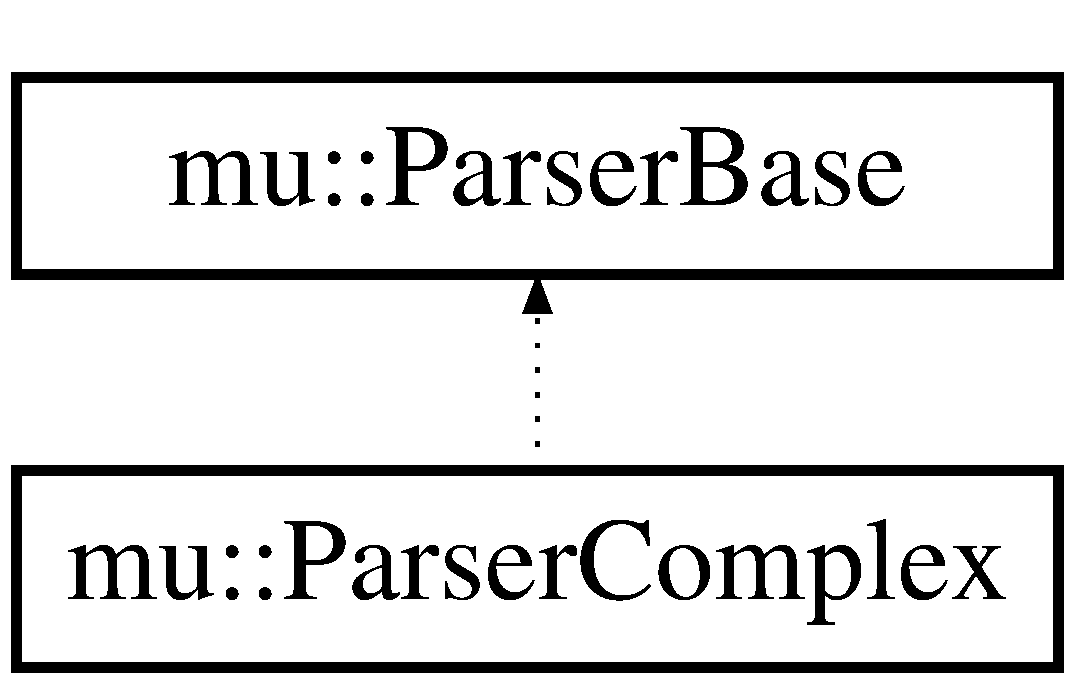
\includegraphics[height=2cm]{classmu_1_1ParserComplex}
\end{center}
\end{figure}


\subsection{Detailed Description}
Mathematical expressions parser. 

This version of the parser handles only complex numbers. It disables the built in operators thus it is slower than muParser. \subsection*{Public Types}
\begin{CompactItemize}
\item 
typedef std::complex$<$ float $>$ {\bf complex\_\-type}
\end{CompactItemize}
\subsection*{Public Member Functions}
\begin{CompactItemize}
\item 
{\bf ParserComplex} ()
\begin{CompactList}\small\item\em Constructor. \item\end{CompactList}\item 
{\bf complex\_\-type} {\bf Eval} ()
\end{CompactItemize}


\subsection{Member Typedef Documentation}
\index{mu::ParserComplex@{mu::ParserComplex}!complex\_\-type@{complex\_\-type}}
\index{complex\_\-type@{complex\_\-type}!mu::ParserComplex@{mu::ParserComplex}}
\subsubsection[complex\_\-type]{\setlength{\rightskip}{0pt plus 5cm}typedef std::complex$<$float$>$ {\bf mu::ParserComplex::complex\_\-type}}\label{classmu_1_1ParserComplex_669d2145497f21c0cd69989c09462789}




\subsection{Constructor \& Destructor Documentation}
\index{mu::ParserComplex@{mu::ParserComplex}!ParserComplex@{ParserComplex}}
\index{ParserComplex@{ParserComplex}!mu::ParserComplex@{mu::ParserComplex}}
\subsubsection[ParserComplex]{\setlength{\rightskip}{0pt plus 5cm}mu::ParserComplex::ParserComplex ()}\label{classmu_1_1ParserComplex_1e34329a17ed3cf64d5463a2e63206b9}


Constructor. 

Call \doxyref{ParserBase}{p.}{classmu_1_1ParserBase} class constructor and trigger Function, Operator and Constant initialization. 

References mu::ParserBase::AddValIdent().

\subsection{Member Function Documentation}
\index{mu::ParserComplex@{mu::ParserComplex}!Eval@{Eval}}
\index{Eval@{Eval}!mu::ParserComplex@{mu::ParserComplex}}
\subsubsection[Eval]{\setlength{\rightskip}{0pt plus 5cm}{\bf ParserComplex::complex\_\-type} mu::ParserComplex::Eval ()}\label{classmu_1_1ParserComplex_ac0f5ef965b1e66c38741b370446f246}




References mu::ParserBase::Eval().

The documentation for this class was generated from the following files:\begin{CompactItemize}
\item 
{\bf muParserComplex.h}\item 
{\bf muParserComplex.cpp}\end{CompactItemize}

\section{mu::ParserError Class Reference}
\label{classmu_1_1ParserError}\index{mu::ParserError@{mu::ParserError}}
{\tt \#include $<$muParserError.h$>$}



\subsection{Detailed Description}
Error class of the parser. 

Part of the math parser package.

\begin{Desc}
\item[Author:]Ingo Berg \end{Desc}
\subsection*{Public Member Functions}
\begin{CompactItemize}
\item 
{\bf ParserError} ()
\begin{CompactList}\small\item\em Default constructor. \item\end{CompactList}\item 
{\bf ParserError} ({\bf EErrorCodes} a\_\-iErrc)
\begin{CompactList}\small\item\em This Constructor is used for internal exceptions only. \item\end{CompactList}\item 
{\bf ParserError} (const {\bf string\_\-type} \&sMsg)
\begin{CompactList}\small\item\em Construct an error from a message text. \item\end{CompactList}\item 
{\bf ParserError} ({\bf EErrorCodes} a\_\-iErrc, const {\bf string\_\-type} \&sTok, const {\bf string\_\-type} \&sFormula={\bf string\_\-type}(\_\-T(\char`\"{}(formula is not available)\char`\"{})), int a\_\-iPos=-1)
\begin{CompactList}\small\item\em Construct an error object. \item\end{CompactList}\item 
{\bf ParserError} ({\bf EErrorCodes} a\_\-iErrc, int a\_\-iPos, const {\bf string\_\-type} \&sTok)
\begin{CompactList}\small\item\em Construct an error object. \item\end{CompactList}\item 
{\bf ParserError} (const {\bf char\_\-type} $\ast$a\_\-szMsg, int a\_\-iPos=-1, const {\bf string\_\-type} \&sTok={\bf string\_\-type}())
\begin{CompactList}\small\item\em Construct an error object. \item\end{CompactList}\item 
{\bf ParserError} (const {\bf ParserError} \&a\_\-Obj)
\begin{CompactList}\small\item\em Copy constructor. \item\end{CompactList}\item 
{\bf ParserError} \& {\bf operator=} (const {\bf ParserError} \&a\_\-Obj)
\begin{CompactList}\small\item\em Assignment operator. \item\end{CompactList}\item 
{\bf $\sim$ParserError} ()
\item 
void {\bf SetFormula} (const {\bf string\_\-type} \&a\_\-strFormula)
\begin{CompactList}\small\item\em Set the expression related to this error. \item\end{CompactList}\item 
const {\bf string\_\-type} \& {\bf GetExpr} () const 
\begin{CompactList}\small\item\em gets the expression related tp this error. \item\end{CompactList}\item 
const {\bf string\_\-type} \& {\bf GetMsg} () const 
\begin{CompactList}\small\item\em Returns the message string for this error. \item\end{CompactList}\item 
std::size\_\-t {\bf GetPos} () const 
\begin{CompactList}\small\item\em Return the formula position related to the error. \item\end{CompactList}\item 
const {\bf string\_\-type} \& {\bf GetToken} () const 
\begin{CompactList}\small\item\em Return string related with this token (if available). \item\end{CompactList}\item 
{\bf EErrorCodes} {\bf GetCode} () const 
\begin{CompactList}\small\item\em Return the error code. \item\end{CompactList}\end{CompactItemize}


\subsection{Constructor \& Destructor Documentation}
\index{mu::ParserError@{mu::ParserError}!ParserError@{ParserError}}
\index{ParserError@{ParserError}!mu::ParserError@{mu::ParserError}}
\subsubsection[ParserError]{\setlength{\rightskip}{0pt plus 5cm}mu::ParserError::ParserError ()}\label{classmu_1_1ParserError_d7f1fb7501d606308cf41c3eeab49348}


Default constructor. 

\index{mu::ParserError@{mu::ParserError}!ParserError@{ParserError}}
\index{ParserError@{ParserError}!mu::ParserError@{mu::ParserError}}
\subsubsection[ParserError]{\setlength{\rightskip}{0pt plus 5cm}mu::ParserError::ParserError ({\bf EErrorCodes} {\em a\_\-iErrc})\hspace{0.3cm}{\tt  [explicit]}}\label{classmu_1_1ParserError_3f37c865f1c609337114f19525f4e625}


This Constructor is used for internal exceptions only. 

It does not contain any information but the error code. \index{mu::ParserError@{mu::ParserError}!ParserError@{ParserError}}
\index{ParserError@{ParserError}!mu::ParserError@{mu::ParserError}}
\subsubsection[ParserError]{\setlength{\rightskip}{0pt plus 5cm}mu::ParserError::ParserError (const {\bf string\_\-type} \& {\em sMsg})\hspace{0.3cm}{\tt  [explicit]}}\label{classmu_1_1ParserError_67297c47b34173e5a331b3ff964d1bfc}


Construct an error from a message text. 

\index{mu::ParserError@{mu::ParserError}!ParserError@{ParserError}}
\index{ParserError@{ParserError}!mu::ParserError@{mu::ParserError}}
\subsubsection[ParserError]{\setlength{\rightskip}{0pt plus 5cm}mu::ParserError::ParserError ({\bf EErrorCodes} {\em iErrc}, \/  const {\bf string\_\-type} \& {\em sTok}, \/  const {\bf string\_\-type} \& {\em sExpr} = {\tt {\bf string\_\-type}(\_\-T(\char`\"{}(formula~is~not~available)\char`\"{}))}, \/  int {\em iPos} = {\tt -1})}\label{classmu_1_1ParserError_c727d75f4c4f4f4269f0075c47288fe1}


Construct an error object. 

\begin{Desc}
\item[Parameters:]
\begin{description}
\item[\mbox{$\leftarrow$} {\em iErrc}]the error code. \item[\mbox{$\leftarrow$} {\em sTok}]The token string related to this error. \item[\mbox{$\leftarrow$} {\em sExpr}]The expression related to the error. \item[\mbox{$\leftarrow$} {\em iPos}]the position in the expression where the error occured. \end{description}
\end{Desc}
\index{mu::ParserError@{mu::ParserError}!ParserError@{ParserError}}
\index{ParserError@{ParserError}!mu::ParserError@{mu::ParserError}}
\subsubsection[ParserError]{\setlength{\rightskip}{0pt plus 5cm}mu::ParserError::ParserError ({\bf EErrorCodes} {\em iErrc}, \/  int {\em iPos}, \/  const {\bf string\_\-type} \& {\em sTok})}\label{classmu_1_1ParserError_b21ddceddd5ae816abc1060873a245b0}


Construct an error object. 

\begin{Desc}
\item[Parameters:]
\begin{description}
\item[\mbox{$\leftarrow$} {\em iErrc}]the error code. \item[\mbox{$\leftarrow$} {\em iPos}]the position in the expression where the error occured. \item[\mbox{$\leftarrow$} {\em sTok}]The token string related to this error. \end{description}
\end{Desc}
\index{mu::ParserError@{mu::ParserError}!ParserError@{ParserError}}
\index{ParserError@{ParserError}!mu::ParserError@{mu::ParserError}}
\subsubsection[ParserError]{\setlength{\rightskip}{0pt plus 5cm}mu::ParserError::ParserError (const {\bf char\_\-type} $\ast$ {\em szMsg}, \/  int {\em iPos} = {\tt -1}, \/  const {\bf string\_\-type} \& {\em sTok} = {\tt {\bf string\_\-type}()})}\label{classmu_1_1ParserError_c4f83d23ad5875683d4100a85f0fbdfc}


Construct an error object. 

\begin{Desc}
\item[Parameters:]
\begin{description}
\item[\mbox{$\leftarrow$} {\em szMsg}]The error message text. \item[\mbox{$\leftarrow$} {\em iPos}]the position related to the error. \item[\mbox{$\leftarrow$} {\em sTok}]The token string related to this error. \end{description}
\end{Desc}
\index{mu::ParserError@{mu::ParserError}!ParserError@{ParserError}}
\index{ParserError@{ParserError}!mu::ParserError@{mu::ParserError}}
\subsubsection[ParserError]{\setlength{\rightskip}{0pt plus 5cm}mu::ParserError::ParserError (const {\bf ParserError} \& {\em a\_\-Obj})}\label{classmu_1_1ParserError_0820d687ae9ed8eed5bad962b40d006c}


Copy constructor. 

\index{mu::ParserError@{mu::ParserError}!$\sim$ParserError@{$\sim$ParserError}}
\index{$\sim$ParserError@{$\sim$ParserError}!mu::ParserError@{mu::ParserError}}
\subsubsection[$\sim$ParserError]{\setlength{\rightskip}{0pt plus 5cm}mu::ParserError::$\sim$ParserError ()}\label{classmu_1_1ParserError_ee52babeeffcf663365b551c3ea61e1f}




\subsection{Member Function Documentation}
\index{mu::ParserError@{mu::ParserError}!operator=@{operator=}}
\index{operator=@{operator=}!mu::ParserError@{mu::ParserError}}
\subsubsection[operator=]{\setlength{\rightskip}{0pt plus 5cm}{\bf ParserError} \& mu::ParserError::operator= (const {\bf ParserError} \& {\em a\_\-Obj})}\label{classmu_1_1ParserError_e2c28377fa08e425a5f3df2cfa221b33}


Assignment operator. 



References m\_\-iErrc, m\_\-iPos, m\_\-strFormula, m\_\-strMsg, and m\_\-strTok.\index{mu::ParserError@{mu::ParserError}!SetFormula@{SetFormula}}
\index{SetFormula@{SetFormula}!mu::ParserError@{mu::ParserError}}
\subsubsection[SetFormula]{\setlength{\rightskip}{0pt plus 5cm}void mu::ParserError::SetFormula (const {\bf string\_\-type} \& {\em a\_\-strFormula})}\label{classmu_1_1ParserError_1b7b4b511525f13f728c9c2942983b19}


Set the expression related to this error. 

\index{mu::ParserError@{mu::ParserError}!GetExpr@{GetExpr}}
\index{GetExpr@{GetExpr}!mu::ParserError@{mu::ParserError}}
\subsubsection[GetExpr]{\setlength{\rightskip}{0pt plus 5cm}const {\bf string\_\-type} \& mu::ParserError::GetExpr () const}\label{classmu_1_1ParserError_845ae0a3276f1f0326c6b9f4d946bcbf}


gets the expression related tp this error. 

\index{mu::ParserError@{mu::ParserError}!GetMsg@{GetMsg}}
\index{GetMsg@{GetMsg}!mu::ParserError@{mu::ParserError}}
\subsubsection[GetMsg]{\setlength{\rightskip}{0pt plus 5cm}const {\bf string\_\-type} \& mu::ParserError::GetMsg () const}\label{classmu_1_1ParserError_f03a4eb049e106be1dbc957ab4c90ee8}


Returns the message string for this error. 

\index{mu::ParserError@{mu::ParserError}!GetPos@{GetPos}}
\index{GetPos@{GetPos}!mu::ParserError@{mu::ParserError}}
\subsubsection[GetPos]{\setlength{\rightskip}{0pt plus 5cm}std::size\_\-t mu::ParserError::GetPos () const}\label{classmu_1_1ParserError_38fa45df3312a8258b58fa0b25550618}


Return the formula position related to the error. 

If the error is not related to a distinct position this will return -1 \index{mu::ParserError@{mu::ParserError}!GetToken@{GetToken}}
\index{GetToken@{GetToken}!mu::ParserError@{mu::ParserError}}
\subsubsection[GetToken]{\setlength{\rightskip}{0pt plus 5cm}const {\bf string\_\-type} \& mu::ParserError::GetToken () const}\label{classmu_1_1ParserError_3ddb4de710a8b0485e1b4060ccc7f08f}


Return string related with this token (if available). 

\index{mu::ParserError@{mu::ParserError}!GetCode@{GetCode}}
\index{GetCode@{GetCode}!mu::ParserError@{mu::ParserError}}
\subsubsection[GetCode]{\setlength{\rightskip}{0pt plus 5cm}{\bf EErrorCodes} mu::ParserError::GetCode () const}\label{classmu_1_1ParserError_ad82b1aeb00b5e64a56956490febd2ec}


Return the error code. 



The documentation for this class was generated from the following files:\begin{CompactItemize}
\item 
{\bf muParserError.h}\item 
{\bf muParserError.cpp}\end{CompactItemize}

\section{mu::ParserErrorMsg Class Reference}
\label{classmu_1_1ParserErrorMsg}\index{mu::ParserErrorMsg@{mu::ParserErrorMsg}}
{\tt \#include $<$muParserError.h$>$}



\subsection{Detailed Description}
A class that handles the error messages. \subsection*{Public Types}
\begin{CompactItemize}
\item 
typedef {\bf ParserErrorMsg} {\bf self\_\-type}
\end{CompactItemize}
\subsection*{Public Member Functions}
\begin{CompactItemize}
\item 
{\bf ParserErrorMsg} \& {\bf operator=} (const {\bf ParserErrorMsg} \&)
\begin{CompactList}\small\item\em Assignement operator is deactivated. \item\end{CompactList}\item 
{\bf ParserErrorMsg} (const {\bf ParserErrorMsg} \&)
\item 
{\bf ParserErrorMsg} ()
\item 
{\bf $\sim$ParserErrorMsg} ()
\item 
{\bf string\_\-type} {\bf operator[$\,$]} (unsigned a\_\-iIdx) const 
\end{CompactItemize}
\subsection*{Static Public Member Functions}
\begin{CompactItemize}
\item 
static const {\bf ParserErrorMsg} \& {\bf Instance} ()
\end{CompactItemize}


\subsection{Member Typedef Documentation}
\index{mu::ParserErrorMsg@{mu::ParserErrorMsg}!self\_\-type@{self\_\-type}}
\index{self\_\-type@{self\_\-type}!mu::ParserErrorMsg@{mu::ParserErrorMsg}}
\subsubsection[self\_\-type]{\setlength{\rightskip}{0pt plus 5cm}typedef {\bf ParserErrorMsg} {\bf mu::ParserErrorMsg::self\_\-type}}\label{classmu_1_1ParserErrorMsg_021c69b193a67c3f907d94648a2c23ef}




\subsection{Constructor \& Destructor Documentation}
\index{mu::ParserErrorMsg@{mu::ParserErrorMsg}!ParserErrorMsg@{ParserErrorMsg}}
\index{ParserErrorMsg@{ParserErrorMsg}!mu::ParserErrorMsg@{mu::ParserErrorMsg}}
\subsubsection[ParserErrorMsg]{\setlength{\rightskip}{0pt plus 5cm}mu::ParserErrorMsg::ParserErrorMsg (const {\bf ParserErrorMsg} \&)}\label{classmu_1_1ParserErrorMsg_3582c28dc06a0c08f6ddcba2c423491e}


\index{mu::ParserErrorMsg@{mu::ParserErrorMsg}!ParserErrorMsg@{ParserErrorMsg}}
\index{ParserErrorMsg@{ParserErrorMsg}!mu::ParserErrorMsg@{mu::ParserErrorMsg}}
\subsubsection[ParserErrorMsg]{\setlength{\rightskip}{0pt plus 5cm}mu::ParserErrorMsg::ParserErrorMsg ()}\label{classmu_1_1ParserErrorMsg_ac3208ea3586efee10cd75ee6f42ee25}




References mu::ecBUILTIN\_\-OVERLOAD, mu::ecCOUNT, mu::ecDIV\_\-BY\_\-ZERO, mu::ecDOMAIN\_\-ERROR, mu::ecEMPTY\_\-EXPRESSION, mu::ecGENERIC, mu::ecINTERNAL\_\-ERROR, mu::ecINVALID\_\-FUN\_\-PTR, mu::ecINVALID\_\-NAME, mu::ecINVALID\_\-VAR\_\-PTR, mu::ecLOCALE, mu::ecMISSING\_\-PARENS, mu::ecNAME\_\-CONFLICT, mu::ecOPRT\_\-TYPE\_\-CONFLICT, mu::ecOPT\_\-PRI, mu::ecSTR\_\-RESULT, mu::ecSTRING\_\-EXPECTED, mu::ecTOO\_\-FEW\_\-PARAMS, mu::ecTOO\_\-MANY\_\-PARAMS, mu::ecUNASSIGNABLE\_\-TOKEN, mu::ecUNEXPECTED\_\-ARG, mu::ecUNEXPECTED\_\-ARG\_\-SEP, mu::ecUNEXPECTED\_\-EOF, mu::ecUNEXPECTED\_\-FUN, mu::ecUNEXPECTED\_\-OPERATOR, mu::ecUNEXPECTED\_\-PARENS, mu::ecUNEXPECTED\_\-STR, mu::ecUNEXPECTED\_\-VAL, mu::ecUNEXPECTED\_\-VAR, mu::ecUNTERMINATED\_\-STRING, and mu::ecVAL\_\-EXPECTED.\index{mu::ParserErrorMsg@{mu::ParserErrorMsg}!$\sim$ParserErrorMsg@{$\sim$ParserErrorMsg}}
\index{$\sim$ParserErrorMsg@{$\sim$ParserErrorMsg}!mu::ParserErrorMsg@{mu::ParserErrorMsg}}
\subsubsection[$\sim$ParserErrorMsg]{\setlength{\rightskip}{0pt plus 5cm}mu::ParserErrorMsg::$\sim$ParserErrorMsg ()}\label{classmu_1_1ParserErrorMsg_3d00e0f669c764e8d75509e8d6152d7b}




\subsection{Member Function Documentation}
\index{mu::ParserErrorMsg@{mu::ParserErrorMsg}!operator=@{operator=}}
\index{operator=@{operator=}!mu::ParserErrorMsg@{mu::ParserErrorMsg}}
\subsubsection[operator=]{\setlength{\rightskip}{0pt plus 5cm}{\bf ParserErrorMsg} \& mu::ParserErrorMsg::operator= (const {\bf ParserErrorMsg} \&)}\label{classmu_1_1ParserErrorMsg_032500259ac54ce82fb08f696f07f2d7}


Assignement operator is deactivated. 

\index{mu::ParserErrorMsg@{mu::ParserErrorMsg}!Instance@{Instance}}
\index{Instance@{Instance}!mu::ParserErrorMsg@{mu::ParserErrorMsg}}
\subsubsection[Instance]{\setlength{\rightskip}{0pt plus 5cm}const {\bf ParserErrorMsg} \& mu::ParserErrorMsg::Instance ()\hspace{0.3cm}{\tt  [static]}}\label{classmu_1_1ParserErrorMsg_3ffa52ec8676870b4af280ccd62ec329}


\index{mu::ParserErrorMsg@{mu::ParserErrorMsg}!operator[]@{operator[]}}
\index{operator[]@{operator[]}!mu::ParserErrorMsg@{mu::ParserErrorMsg}}
\subsubsection[operator[]]{\setlength{\rightskip}{0pt plus 5cm}{\bf string\_\-type} mu::ParserErrorMsg::operator[$\,$] (unsigned {\em a\_\-iIdx}) const}\label{classmu_1_1ParserErrorMsg_50b72ec4614d582045fa97c273b2e4ff}




The documentation for this class was generated from the following files:\begin{CompactItemize}
\item 
{\bf muParserError.h}\item 
{\bf muParserError.cpp}\end{CompactItemize}

\section{mu::ParserInt Class Reference}
\label{classmu_1_1ParserInt}\index{mu::ParserInt@{mu::ParserInt}}
{\tt \#include $<$muParserInt.h$>$}

Inheritance diagram for mu::ParserInt::\begin{figure}[H]
\begin{center}
\leavevmode
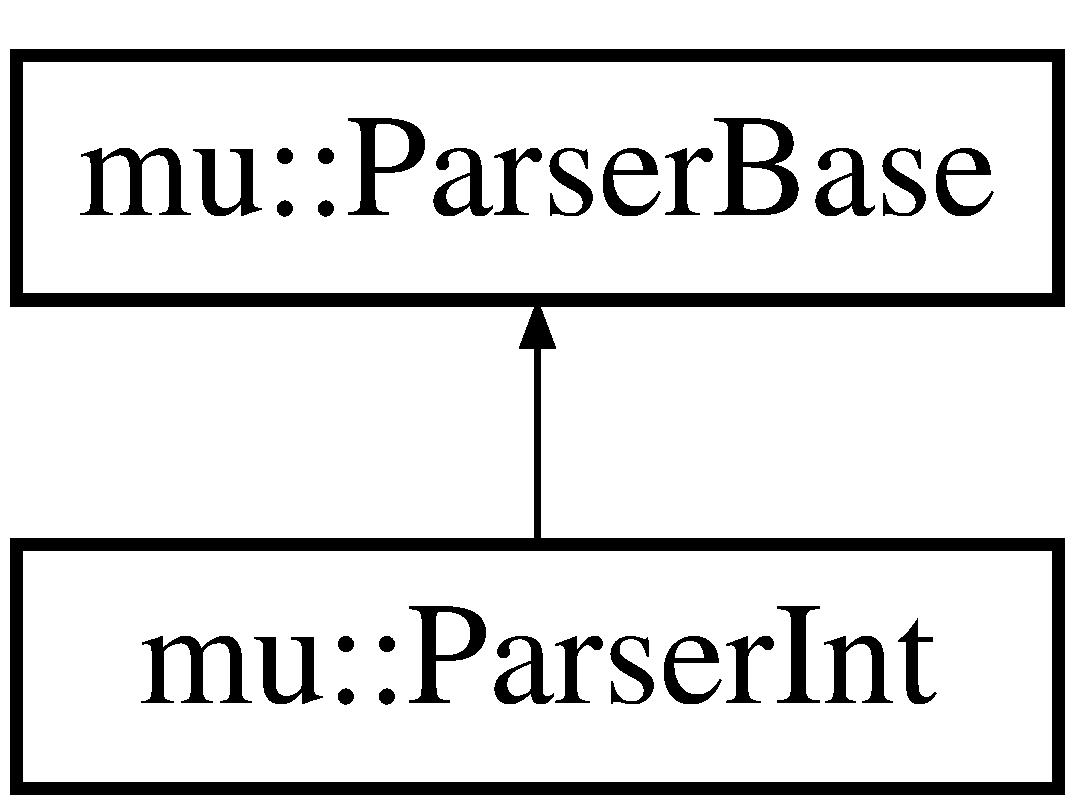
\includegraphics[height=2cm]{classmu_1_1ParserInt}
\end{center}
\end{figure}


\subsection{Detailed Description}
Mathematical expressions parser. 

This version of the parser handles only integer numbers. It disables the built in operators thus it is slower than muParser. Integer values are stored in the double value\_\-type and converted if needed. \subsection*{Public Member Functions}
\begin{CompactItemize}
\item 
{\bf ParserInt} ()
\begin{CompactList}\small\item\em Constructor. \item\end{CompactList}\item 
virtual void {\bf InitFun} ()
\begin{CompactList}\small\item\em Initialize the default functions. \item\end{CompactList}\item 
virtual void {\bf InitOprt} ()
\begin{CompactList}\small\item\em Initialize operators. \item\end{CompactList}\item 
virtual void {\bf InitConst} ()
\item 
virtual void {\bf InitCharSets} ()
\end{CompactItemize}


\subsection{Constructor \& Destructor Documentation}
\index{mu::ParserInt@{mu::ParserInt}!ParserInt@{ParserInt}}
\index{ParserInt@{ParserInt}!mu::ParserInt@{mu::ParserInt}}
\subsubsection[ParserInt]{\setlength{\rightskip}{0pt plus 5cm}mu::ParserInt::ParserInt ()}\label{classmu_1_1ParserInt_2e2776f16a30d3f1aa698437f7c4cb5f}


Constructor. 

Call \doxyref{ParserBase}{p.}{classmu_1_1ParserBase} class constructor and trigger Function, Operator and Constant initialization. 

References mu::ParserBase::AddValIdent(), InitCharSets(), InitFun(), and InitOprt().

\subsection{Member Function Documentation}
\index{mu::ParserInt@{mu::ParserInt}!InitFun@{InitFun}}
\index{InitFun@{InitFun}!mu::ParserInt@{mu::ParserInt}}
\subsubsection[InitFun]{\setlength{\rightskip}{0pt plus 5cm}void mu::ParserInt::InitFun ()\hspace{0.3cm}{\tt  [virtual]}}\label{classmu_1_1ParserInt_f7aa0bcbee6abf01676a3615206f14de}


Initialize the default functions. 



Implements {\bf mu::ParserBase} \doxyref{}{p.}{classmu_1_1ParserBase_1f94305e7b7e9abff6d41242dcf188ed}.

Referenced by ParserInt().\index{mu::ParserInt@{mu::ParserInt}!InitOprt@{InitOprt}}
\index{InitOprt@{InitOprt}!mu::ParserInt@{mu::ParserInt}}
\subsubsection[InitOprt]{\setlength{\rightskip}{0pt plus 5cm}void mu::ParserInt::InitOprt ()\hspace{0.3cm}{\tt  [virtual]}}\label{classmu_1_1ParserInt_9bc5fc5f5be541a2329952138ad933e9}


Initialize operators. 



Implements {\bf mu::ParserBase} \doxyref{}{p.}{classmu_1_1ParserBase_4df16813c9002ff08c96929ba8f0d32b}.

References mu::ParserBase::DefineInfixOprt(), mu::ParserBase::DefineOprt(), mu::ParserBase::EnableBuiltInOprt(), mu::prADD\_\-SUB, mu::prCMP, mu::prLOGIC, and mu::prMUL\_\-DIV.

Referenced by ParserInt().\index{mu::ParserInt@{mu::ParserInt}!InitConst@{InitConst}}
\index{InitConst@{InitConst}!mu::ParserInt@{mu::ParserInt}}
\subsubsection[InitConst]{\setlength{\rightskip}{0pt plus 5cm}void mu::ParserInt::InitConst ()\hspace{0.3cm}{\tt  [virtual]}}\label{classmu_1_1ParserInt_4c59df078eecbe6ac79749271463b400}




Implements {\bf mu::ParserBase} \doxyref{}{p.}{classmu_1_1ParserBase_ad904fb3df8f28659f36d7ce7db4a28c}.\index{mu::ParserInt@{mu::ParserInt}!InitCharSets@{InitCharSets}}
\index{InitCharSets@{InitCharSets}!mu::ParserInt@{mu::ParserInt}}
\subsubsection[InitCharSets]{\setlength{\rightskip}{0pt plus 5cm}void mu::ParserInt::InitCharSets ()\hspace{0.3cm}{\tt  [virtual]}}\label{classmu_1_1ParserInt_a9589acaa68c3341490ae51bca9b0e78}




Implements {\bf mu::ParserBase} \doxyref{}{p.}{classmu_1_1ParserBase_3f5c53ef3cba6ab939261677dc2d9709}.

References mu::ParserBase::DefineInfixOprtChars(), mu::ParserBase::DefineNameChars(), and mu::ParserBase::DefineOprtChars().

Referenced by ParserInt().

The documentation for this class was generated from the following files:\begin{CompactItemize}
\item 
{\bf muParserInt.h}\item 
{\bf muParserInt.cpp}\end{CompactItemize}

\section{mu::ParserStack$<$ TValueType $>$ Class Template Reference}
\label{classmu_1_1ParserStack}\index{mu::ParserStack@{mu::ParserStack}}
{\tt \#include $<$muParserStack.h$>$}



\subsection{Detailed Description}
\subsubsection*{template$<$typename TValueType$>$ class mu::ParserStack$<$ TValueType $>$}

\doxyref{Parser}{p.}{classmu_1_1Parser} stack implementation. 

Stack implementation based on a std::stack. The behaviour of \doxyref{pop()}{p.}{classmu_1_1ParserStack_d00f833ee3f30d901fa18e714105c381} had been slightly changed in order to get an error code if the stack is empty. The stack is used within the \doxyref{Parser}{p.}{classmu_1_1Parser} both as a value stack and as an operator stack.

\begin{Desc}
\item[Author:](C) 2004-2008 Ingo Berg \end{Desc}
\subsection*{Public Member Functions}
\begin{CompactItemize}
\item 
{\bf ParserStack} ()
\item 
virtual {\bf $\sim$ParserStack} ()
\item 
TValueType {\bf pop} ()
\begin{CompactList}\small\item\em Pop a value from the stack. \item\end{CompactList}\item 
void {\bf push} (const TValueType \&a\_\-Val)
\begin{CompactList}\small\item\em Push an object into the stack. \item\end{CompactList}\item 
unsigned {\bf size} () const 
\begin{CompactList}\small\item\em Return the number of stored elements. \item\end{CompactList}\item 
bool {\bf empty} () const 
\begin{CompactList}\small\item\em Returns true if stack is empty false otherwise. \item\end{CompactList}\item 
TValueType \& {\bf top} ()
\begin{CompactList}\small\item\em Return reference to the top object in the stack. \item\end{CompactList}\end{CompactItemize}


\subsection{Constructor \& Destructor Documentation}
\index{mu::ParserStack@{mu::ParserStack}!ParserStack@{ParserStack}}
\index{ParserStack@{ParserStack}!mu::ParserStack@{mu::ParserStack}}
\subsubsection[ParserStack]{\setlength{\rightskip}{0pt plus 5cm}template$<$typename TValueType$>$ {\bf mu::ParserStack}$<$ TValueType $>$::{\bf ParserStack} ()\hspace{0.3cm}{\tt  [inline]}}\label{classmu_1_1ParserStack_570cdffe52bdaf5c549446509f06ea96}


\index{mu::ParserStack@{mu::ParserStack}!$\sim$ParserStack@{$\sim$ParserStack}}
\index{$\sim$ParserStack@{$\sim$ParserStack}!mu::ParserStack@{mu::ParserStack}}
\subsubsection[$\sim$ParserStack]{\setlength{\rightskip}{0pt plus 5cm}template$<$typename TValueType$>$ virtual {\bf mu::ParserStack}$<$ TValueType $>$::$\sim${\bf ParserStack} ()\hspace{0.3cm}{\tt  [inline, virtual]}}\label{classmu_1_1ParserStack_7ac063affb6991bc6a06e111082a5cfb}




\subsection{Member Function Documentation}
\index{mu::ParserStack@{mu::ParserStack}!pop@{pop}}
\index{pop@{pop}!mu::ParserStack@{mu::ParserStack}}
\subsubsection[pop]{\setlength{\rightskip}{0pt plus 5cm}template$<$typename TValueType$>$ TValueType {\bf mu::ParserStack}$<$ TValueType $>$::pop ()\hspace{0.3cm}{\tt  [inline]}}\label{classmu_1_1ParserStack_d00f833ee3f30d901fa18e714105c381}


Pop a value from the stack. 

Unlike the standard implementation this function will return the value that is going to be taken from the stack.

\begin{Desc}
\item[Exceptions:]
\begin{description}
\item[{\em ParserException}]in case the stack is empty. \end{description}
\end{Desc}
\begin{Desc}
\item[See also:]pop(int \&a\_\-iErrc) \end{Desc}


References mu::ParserStack$<$ TValueType $>$::empty(), and mu::ParserStack$<$ TValueType $>$::top().\index{mu::ParserStack@{mu::ParserStack}!push@{push}}
\index{push@{push}!mu::ParserStack@{mu::ParserStack}}
\subsubsection[push]{\setlength{\rightskip}{0pt plus 5cm}template$<$typename TValueType$>$ void {\bf mu::ParserStack}$<$ TValueType $>$::push (const TValueType \& {\em a\_\-Val})\hspace{0.3cm}{\tt  [inline]}}\label{classmu_1_1ParserStack_38ae431c967a6607aace9dfd4ae4cc5f}


Push an object into the stack. 

\begin{Desc}
\item[Parameters:]
\begin{description}
\item[{\em a\_\-Val}]object to push into the stack. \end{description}
\end{Desc}
\begin{Desc}
\item[Exceptions:]
\begin{description}
\item[{\em nothrow}]\end{description}
\end{Desc}
\index{mu::ParserStack@{mu::ParserStack}!size@{size}}
\index{size@{size}!mu::ParserStack@{mu::ParserStack}}
\subsubsection[size]{\setlength{\rightskip}{0pt plus 5cm}template$<$typename TValueType$>$ unsigned {\bf mu::ParserStack}$<$ TValueType $>$::size () const\hspace{0.3cm}{\tt  [inline]}}\label{classmu_1_1ParserStack_62c1e65a4e0d15f01a031fb245528166}


Return the number of stored elements. 

\index{mu::ParserStack@{mu::ParserStack}!empty@{empty}}
\index{empty@{empty}!mu::ParserStack@{mu::ParserStack}}
\subsubsection[empty]{\setlength{\rightskip}{0pt plus 5cm}template$<$typename TValueType$>$ bool {\bf mu::ParserStack}$<$ TValueType $>$::empty () const\hspace{0.3cm}{\tt  [inline]}}\label{classmu_1_1ParserStack_43464a5bd94c2566b87cabe7d8e83fbb}


Returns true if stack is empty false otherwise. 



Referenced by mu::ParserStack$<$ TValueType $>$::pop().\index{mu::ParserStack@{mu::ParserStack}!top@{top}}
\index{top@{top}!mu::ParserStack@{mu::ParserStack}}
\subsubsection[top]{\setlength{\rightskip}{0pt plus 5cm}template$<$typename TValueType$>$ TValueType\& {\bf mu::ParserStack}$<$ TValueType $>$::top ()\hspace{0.3cm}{\tt  [inline]}}\label{classmu_1_1ParserStack_ba3a499ebaae388c27bfb81883cba7fd}


Return reference to the top object in the stack. 

The top object is the one pushed most recently. 

Referenced by mu::ParserStack$<$ TValueType $>$::pop().

The documentation for this class was generated from the following file:\begin{CompactItemize}
\item 
{\bf muParserStack.h}\end{CompactItemize}

\section{mu::ParserToken$<$ TBase, TString $>$ Class Template Reference}
\label{classmu_1_1ParserToken}\index{mu::ParserToken@{mu::ParserToken}}
{\tt \#include $<$muParserToken.h$>$}



\subsection{Detailed Description}
\subsubsection*{template$<$typename TBase, typename TString$>$ class mu::ParserToken$<$ TBase, TString $>$}

Encapsulation of the data for a single formula token. 

Formula token implementation. Part of the Math \doxyref{Parser}{p.}{classmu_1_1Parser} Package. Formula tokens can be either one of the following: \begin{itemize}
\item value \item variable \item function with numerical arguments \item functions with a string as argument \item prefix operators \item infix operators \item binary operator \end{itemize}


\begin{Desc}
\item[Author:](C) 2004 Ingo Berg \end{Desc}
\subsection*{Public Types}
\begin{CompactItemize}
\item 
enum {\bf ETokFlags} \{ {\bf flVOLATILE} =  1
 \}
\begin{CompactList}\small\item\em Additional token flags. \item\end{CompactList}\end{CompactItemize}
\subsection*{Public Member Functions}
\begin{CompactItemize}
\item 
{\bf ParserToken} ()
\begin{CompactList}\small\item\em Constructor (default). \item\end{CompactList}\item 
{\bf ParserToken} (const {\bf ParserToken} \&a\_\-Tok)
\begin{CompactList}\small\item\em Create token from another one. \item\end{CompactList}\item 
{\bf ParserToken} \& {\bf operator=} (const {\bf ParserToken} \&a\_\-Tok)
\begin{CompactList}\small\item\em Assignement operator. \item\end{CompactList}\item 
void {\bf Assign} (const {\bf ParserToken} \&a\_\-Tok)
\begin{CompactList}\small\item\em Copy token information from argument. \item\end{CompactList}\item 
void {\bf AddFlags} (int a\_\-iFlags)
\begin{CompactList}\small\item\em Add additional flags to the token. \item\end{CompactList}\item 
bool {\bf IsFlagSet} (int a\_\-iFlags) const 
\begin{CompactList}\small\item\em Check if a certain flag ist set. \item\end{CompactList}\item 
{\bf ParserToken} \& {\bf Set} ({\bf ECmdCode} a\_\-iType, const TString \&a\_\-strTok=TString())
\begin{CompactList}\small\item\em Assign a token type. \item\end{CompactList}\item 
{\bf ParserToken} \& {\bf Set} (const {\bf ParserCallback} \&a\_\-pCallback, const TString \&a\_\-sTok)
\begin{CompactList}\small\item\em Set Callback type. \item\end{CompactList}\item 
{\bf ParserToken} \& {\bf SetVal} (TBase a\_\-fVal, const TString \&a\_\-strTok=TString())
\begin{CompactList}\small\item\em Make this token a value token. \item\end{CompactList}\item 
{\bf ParserToken} \& {\bf SetVar} (TBase $\ast$a\_\-pVar, const TString \&a\_\-strTok)
\begin{CompactList}\small\item\em make this token a variable token. \item\end{CompactList}\item 
{\bf ParserToken} \& {\bf SetString} (const TString \&a\_\-strTok, std::size\_\-t a\_\-iSize)
\begin{CompactList}\small\item\em Make this token a variable token. \item\end{CompactList}\item 
void {\bf SetIdx} (int a\_\-iIdx)
\begin{CompactList}\small\item\em Set an index associated with the token related data. \item\end{CompactList}\item 
int {\bf GetIdx} () const 
\begin{CompactList}\small\item\em Return Index associated with the token related data. \item\end{CompactList}\item 
{\bf ECmdCode} {\bf GetCode} () const 
\begin{CompactList}\small\item\em Return the token type. \item\end{CompactList}\item 
{\bf ETypeCode} {\bf GetType} () const 
\item 
int {\bf GetPri} () const 
\item 
void $\ast$ {\bf GetFuncAddr} () const 
\begin{CompactList}\small\item\em Return the address of the callback function assoziated with function and operator tokens. \item\end{CompactList}\item 
TBase {\bf GetVal} () const 
\item 
TBase $\ast$ {\bf GetVar} () const 
\begin{CompactList}\small\item\em Get address of a variable token. \item\end{CompactList}\item 
int {\bf GetArgCount} () const 
\begin{CompactList}\small\item\em Return the number of function arguments. \item\end{CompactList}\item 
const TString \& {\bf GetAsString} () const 
\begin{CompactList}\small\item\em Return the token identifier. \item\end{CompactList}\end{CompactItemize}


\subsection{Member Enumeration Documentation}
\index{mu::ParserToken@{mu::ParserToken}!ETokFlags@{ETokFlags}}
\index{ETokFlags@{ETokFlags}!mu::ParserToken@{mu::ParserToken}}
\subsubsection[ETokFlags]{\setlength{\rightskip}{0pt plus 5cm}template$<$typename TBase, typename TString$>$ enum {\bf mu::ParserToken::ETokFlags}}\label{classmu_1_1ParserToken_eab15fb29d55a8c525a790f32c837aca}


Additional token flags. 

\begin{Desc}
\item[Enumerator: ]\par
\begin{description}
\index{flVOLATILE@{flVOLATILE}!mu::ParserToken@{mu::ParserToken}}\index{mu::ParserToken@{mu::ParserToken}!flVOLATILE@{flVOLATILE}}\item[{\em 
flVOLATILE\label{classmu_1_1ParserToken_eab15fb29d55a8c525a790f32c837aca7b72b53078f838e624f21bf521b5c5d1}
}]Mark a token that depends on a variable or a function that is not conservative. \end{description}
\end{Desc}



\subsection{Constructor \& Destructor Documentation}
\index{mu::ParserToken@{mu::ParserToken}!ParserToken@{ParserToken}}
\index{ParserToken@{ParserToken}!mu::ParserToken@{mu::ParserToken}}
\subsubsection[ParserToken]{\setlength{\rightskip}{0pt plus 5cm}template$<$typename TBase, typename TString$>$ {\bf mu::ParserToken}$<$ TBase, TString $>$::{\bf ParserToken} ()\hspace{0.3cm}{\tt  [inline]}}\label{classmu_1_1ParserToken_0ce34ca6a1833441e8fd9840b3cde140}


Constructor (default). 

Sets token to an neutral state of type cmUNKNOWN. \begin{Desc}
\item[Exceptions:]
\begin{description}
\item[{\em nothrow}]\end{description}
\end{Desc}
\begin{Desc}
\item[See also:]\doxyref{ECmdCode}{p.}{namespacemu_b77181e591bebd278bf9c7a2e30ad40e} \end{Desc}
\index{mu::ParserToken@{mu::ParserToken}!ParserToken@{ParserToken}}
\index{ParserToken@{ParserToken}!mu::ParserToken@{mu::ParserToken}}
\subsubsection[ParserToken]{\setlength{\rightskip}{0pt plus 5cm}template$<$typename TBase, typename TString$>$ {\bf mu::ParserToken}$<$ TBase, TString $>$::{\bf ParserToken} (const {\bf ParserToken}$<$ TBase, TString $>$ \& {\em a\_\-Tok})\hspace{0.3cm}{\tt  [inline]}}\label{classmu_1_1ParserToken_17dfc71fe5750f61e9cdd5c2a3355ac0}


Create token from another one. 

Implemented by calling Assign(...) \begin{Desc}
\item[Exceptions:]
\begin{description}
\item[{\em nothrow}]\end{description}
\end{Desc}
\begin{Desc}
\item[Postcondition:]m\_\-iType==cmUNKNOWN \end{Desc}
\begin{Desc}
\item[See also:]\doxyref{Assign}{p.}{classmu_1_1ParserToken_40b7e717927c58d03a6665184ff5cc52} \end{Desc}


\subsection{Member Function Documentation}
\index{mu::ParserToken@{mu::ParserToken}!operator=@{operator=}}
\index{operator=@{operator=}!mu::ParserToken@{mu::ParserToken}}
\subsubsection[operator=]{\setlength{\rightskip}{0pt plus 5cm}template$<$typename TBase, typename TString$>$ {\bf ParserToken}\& {\bf mu::ParserToken}$<$ TBase, TString $>$::operator= (const {\bf ParserToken}$<$ TBase, TString $>$ \& {\em a\_\-Tok})\hspace{0.3cm}{\tt  [inline]}}\label{classmu_1_1ParserToken_f9abe46bd0a5f2b4cbcc59beba68ca0e}


Assignement operator. 

Copy token state from another token and return this. Implemented by calling Assign(...). \begin{Desc}
\item[Exceptions:]
\begin{description}
\item[{\em nothrow}]\end{description}
\end{Desc}
\index{mu::ParserToken@{mu::ParserToken}!Assign@{Assign}}
\index{Assign@{Assign}!mu::ParserToken@{mu::ParserToken}}
\subsubsection[Assign]{\setlength{\rightskip}{0pt plus 5cm}template$<$typename TBase, typename TString$>$ void {\bf mu::ParserToken}$<$ TBase, TString $>$::Assign (const {\bf ParserToken}$<$ TBase, TString $>$ \& {\em a\_\-Tok})\hspace{0.3cm}{\tt  [inline]}}\label{classmu_1_1ParserToken_40b7e717927c58d03a6665184ff5cc52}


Copy token information from argument. 

\begin{Desc}
\item[Exceptions:]
\begin{description}
\item[{\em nothrow}]\end{description}
\end{Desc}


Referenced by mu::ParserToken$<$ MUP\_\-BASETYPE, MUP\_\-STRING\_\-TYPE $>$::operator=(), and mu::ParserToken$<$ MUP\_\-BASETYPE, MUP\_\-STRING\_\-TYPE $>$::ParserToken().\index{mu::ParserToken@{mu::ParserToken}!AddFlags@{AddFlags}}
\index{AddFlags@{AddFlags}!mu::ParserToken@{mu::ParserToken}}
\subsubsection[AddFlags]{\setlength{\rightskip}{0pt plus 5cm}template$<$typename TBase, typename TString$>$ void {\bf mu::ParserToken}$<$ TBase, TString $>$::AddFlags (int {\em a\_\-iFlags})\hspace{0.3cm}{\tt  [inline]}}\label{classmu_1_1ParserToken_8b9d1e7d43bf04702540262598536ada}


Add additional flags to the token. 

Flags are currently used to mark volatile (non optimizeable) functions. \begin{Desc}
\item[See also:]m\_\-iFlags, \doxyref{ETokFlags}{p.}{classmu_1_1ParserToken_eab15fb29d55a8c525a790f32c837aca} \end{Desc}


Referenced by mu::ParserToken$<$ MUP\_\-BASETYPE, MUP\_\-STRING\_\-TYPE $>$::Set(), mu::ParserToken$<$ MUP\_\-BASETYPE, MUP\_\-STRING\_\-TYPE $>$::SetString(), and mu::ParserToken$<$ MUP\_\-BASETYPE, MUP\_\-STRING\_\-TYPE $>$::SetVar().\index{mu::ParserToken@{mu::ParserToken}!IsFlagSet@{IsFlagSet}}
\index{IsFlagSet@{IsFlagSet}!mu::ParserToken@{mu::ParserToken}}
\subsubsection[IsFlagSet]{\setlength{\rightskip}{0pt plus 5cm}template$<$typename TBase, typename TString$>$ bool {\bf mu::ParserToken}$<$ TBase, TString $>$::IsFlagSet (int {\em a\_\-iFlags}) const\hspace{0.3cm}{\tt  [inline]}}\label{classmu_1_1ParserToken_7f942072a1f92eb99b2994a7ea85645c}


Check if a certain flag ist set. 

\begin{Desc}
\item[Exceptions:]
\begin{description}
\item[{\em nothrow}]\end{description}
\end{Desc}
\index{mu::ParserToken@{mu::ParserToken}!Set@{Set}}
\index{Set@{Set}!mu::ParserToken@{mu::ParserToken}}
\subsubsection[Set]{\setlength{\rightskip}{0pt plus 5cm}template$<$typename TBase, typename TString$>$ {\bf ParserToken}\& {\bf mu::ParserToken}$<$ TBase, TString $>$::Set ({\bf ECmdCode} {\em a\_\-iType}, \/  const TString \& {\em a\_\-strTok} = {\tt TString()})\hspace{0.3cm}{\tt  [inline]}}\label{classmu_1_1ParserToken_c4588ba38ccc660686956f7998ba74dc}


Assign a token type. 

Token may not be of type value, variable or function. Those have seperate set functions.

\begin{Desc}
\item[Precondition:][assert] a\_\-iType!=cmVAR 

[assert] a\_\-iType!=cmVAL 

[assert] a\_\-iType!=cmFUNC \end{Desc}
\begin{Desc}
\item[Postcondition:]m\_\-fVal = 0 

m\_\-pTok = 0 \end{Desc}
\index{mu::ParserToken@{mu::ParserToken}!Set@{Set}}
\index{Set@{Set}!mu::ParserToken@{mu::ParserToken}}
\subsubsection[Set]{\setlength{\rightskip}{0pt plus 5cm}template$<$typename TBase, typename TString$>$ {\bf ParserToken}\& {\bf mu::ParserToken}$<$ TBase, TString $>$::Set (const {\bf ParserCallback} \& {\em a\_\-pCallback}, \/  const TString \& {\em a\_\-sTok})\hspace{0.3cm}{\tt  [inline]}}\label{classmu_1_1ParserToken_a7c0c0e307b2064f1ab12cbf922c7e40}


Set Callback type. 

\index{mu::ParserToken@{mu::ParserToken}!SetVal@{SetVal}}
\index{SetVal@{SetVal}!mu::ParserToken@{mu::ParserToken}}
\subsubsection[SetVal]{\setlength{\rightskip}{0pt plus 5cm}template$<$typename TBase, typename TString$>$ {\bf ParserToken}\& {\bf mu::ParserToken}$<$ TBase, TString $>$::SetVal (TBase {\em a\_\-fVal}, \/  const TString \& {\em a\_\-strTok} = {\tt TString()})\hspace{0.3cm}{\tt  [inline]}}\label{classmu_1_1ParserToken_68d4974b234ee9f109ef466cd04e1501}


Make this token a value token. 

Member variables not necessary for value tokens will be invalidated. \begin{Desc}
\item[Exceptions:]
\begin{description}
\item[{\em nothrow}]\end{description}
\end{Desc}
\index{mu::ParserToken@{mu::ParserToken}!SetVar@{SetVar}}
\index{SetVar@{SetVar}!mu::ParserToken@{mu::ParserToken}}
\subsubsection[SetVar]{\setlength{\rightskip}{0pt plus 5cm}template$<$typename TBase, typename TString$>$ {\bf ParserToken}\& {\bf mu::ParserToken}$<$ TBase, TString $>$::SetVar (TBase $\ast$ {\em a\_\-pVar}, \/  const TString \& {\em a\_\-strTok})\hspace{0.3cm}{\tt  [inline]}}\label{classmu_1_1ParserToken_86de84eb76900ca677c3ab93681ec7c5}


make this token a variable token. 

Member variables not necessary for variable tokens will be invalidated. \begin{Desc}
\item[Exceptions:]
\begin{description}
\item[{\em nothrow}]\end{description}
\end{Desc}
\index{mu::ParserToken@{mu::ParserToken}!SetString@{SetString}}
\index{SetString@{SetString}!mu::ParserToken@{mu::ParserToken}}
\subsubsection[SetString]{\setlength{\rightskip}{0pt plus 5cm}template$<$typename TBase, typename TString$>$ {\bf ParserToken}\& {\bf mu::ParserToken}$<$ TBase, TString $>$::SetString (const TString \& {\em a\_\-strTok}, \/  std::size\_\-t {\em a\_\-iSize})\hspace{0.3cm}{\tt  [inline]}}\label{classmu_1_1ParserToken_da40ff914f9c59f6891f6809991b3542}


Make this token a variable token. 

Member variables not necessary for variable tokens will be invalidated. \begin{Desc}
\item[Exceptions:]
\begin{description}
\item[{\em nothrow}]\end{description}
\end{Desc}
\index{mu::ParserToken@{mu::ParserToken}!SetIdx@{SetIdx}}
\index{SetIdx@{SetIdx}!mu::ParserToken@{mu::ParserToken}}
\subsubsection[SetIdx]{\setlength{\rightskip}{0pt plus 5cm}template$<$typename TBase, typename TString$>$ void {\bf mu::ParserToken}$<$ TBase, TString $>$::SetIdx (int {\em a\_\-iIdx})\hspace{0.3cm}{\tt  [inline]}}\label{classmu_1_1ParserToken_c2e70ba039bc033722ea946342649881}


Set an index associated with the token related data. 

In cmSTRFUNC - This is the index to a string table in the main parser. parameter: a\_\-iIdx The index the string function result will take in the bytecode parser. \begin{Desc}
\item[Exceptions:]
\begin{description}
\item[{\em exception\_\-type}]if a\_\-iIdx$<$0 or m\_\-iType!=cmSTRING \end{description}
\end{Desc}
\index{mu::ParserToken@{mu::ParserToken}!GetIdx@{GetIdx}}
\index{GetIdx@{GetIdx}!mu::ParserToken@{mu::ParserToken}}
\subsubsection[GetIdx]{\setlength{\rightskip}{0pt plus 5cm}template$<$typename TBase, typename TString$>$ int {\bf mu::ParserToken}$<$ TBase, TString $>$::GetIdx () const\hspace{0.3cm}{\tt  [inline]}}\label{classmu_1_1ParserToken_394d2f4c77548e20d6ea1d69ab583426}


Return Index associated with the token related data. 

In cmSTRFUNC - This is the index to a string table in the main parser.

\begin{Desc}
\item[Exceptions:]
\begin{description}
\item[{\em exception\_\-type}]if m\_\-iIdx$<$0 or m\_\-iType!=cmSTRING \end{description}
\end{Desc}
\begin{Desc}
\item[Returns:]The index the result will take in the Bytecode calculatin array (m\_\-iIdx). \end{Desc}
\index{mu::ParserToken@{mu::ParserToken}!GetCode@{GetCode}}
\index{GetCode@{GetCode}!mu::ParserToken@{mu::ParserToken}}
\subsubsection[GetCode]{\setlength{\rightskip}{0pt plus 5cm}template$<$typename TBase, typename TString$>$ {\bf ECmdCode} {\bf mu::ParserToken}$<$ TBase, TString $>$::GetCode () const\hspace{0.3cm}{\tt  [inline]}}\label{classmu_1_1ParserToken_2aed855c2686a1a4f7696f373e79d2ba}


Return the token type. 

\begin{Desc}
\item[Returns:]m\_\-iType \end{Desc}
\begin{Desc}
\item[Exceptions:]
\begin{description}
\item[{\em nothrow}]\end{description}
\end{Desc}
\index{mu::ParserToken@{mu::ParserToken}!GetType@{GetType}}
\index{GetType@{GetType}!mu::ParserToken@{mu::ParserToken}}
\subsubsection[GetType]{\setlength{\rightskip}{0pt plus 5cm}template$<$typename TBase, typename TString$>$ {\bf ETypeCode} {\bf mu::ParserToken}$<$ TBase, TString $>$::GetType () const\hspace{0.3cm}{\tt  [inline]}}\label{classmu_1_1ParserToken_8b53010c2405da2908ad3b889798f92a}


\index{mu::ParserToken@{mu::ParserToken}!GetPri@{GetPri}}
\index{GetPri@{GetPri}!mu::ParserToken@{mu::ParserToken}}
\subsubsection[GetPri]{\setlength{\rightskip}{0pt plus 5cm}template$<$typename TBase, typename TString$>$ int {\bf mu::ParserToken}$<$ TBase, TString $>$::GetPri () const\hspace{0.3cm}{\tt  [inline]}}\label{classmu_1_1ParserToken_5b032bb1b4b3f4bfc4908e96a33733bc}


\index{mu::ParserToken@{mu::ParserToken}!GetFuncAddr@{GetFuncAddr}}
\index{GetFuncAddr@{GetFuncAddr}!mu::ParserToken@{mu::ParserToken}}
\subsubsection[GetFuncAddr]{\setlength{\rightskip}{0pt plus 5cm}template$<$typename TBase, typename TString$>$ void$\ast$ {\bf mu::ParserToken}$<$ TBase, TString $>$::GetFuncAddr () const\hspace{0.3cm}{\tt  [inline]}}\label{classmu_1_1ParserToken_bbae24591fa059bbc8266728cb303c46}


Return the address of the callback function assoziated with function and operator tokens. 

\begin{Desc}
\item[Returns:]The pointer stored in m\_\-pTok. \end{Desc}
\begin{Desc}
\item[Exceptions:]
\begin{description}
\item[{\em exception\_\-type}]if token type is non of: \begin{itemize}
\item cmFUNC \item cmSTRFUNC \item cmPOSTOP \item cmINFIXOP \item cmOPRT\_\-BIN \end{itemize}
\end{description}
\end{Desc}
\begin{Desc}
\item[See also:]\doxyref{ECmdCode}{p.}{namespacemu_b77181e591bebd278bf9c7a2e30ad40e} \end{Desc}
\index{mu::ParserToken@{mu::ParserToken}!GetVal@{GetVal}}
\index{GetVal@{GetVal}!mu::ParserToken@{mu::ParserToken}}
\subsubsection[GetVal]{\setlength{\rightskip}{0pt plus 5cm}template$<$typename TBase, typename TString$>$ TBase {\bf mu::ParserToken}$<$ TBase, TString $>$::GetVal () const\hspace{0.3cm}{\tt  [inline]}}\label{classmu_1_1ParserToken_92bdbe69e20244358ff7b8348cee4162}


Get value of the token.

Only applicable to variable and value tokens. \begin{Desc}
\item[Exceptions:]
\begin{description}
\item[{\em exception\_\-type}]if token is no value/variable token. \end{description}
\end{Desc}
\index{mu::ParserToken@{mu::ParserToken}!GetVar@{GetVar}}
\index{GetVar@{GetVar}!mu::ParserToken@{mu::ParserToken}}
\subsubsection[GetVar]{\setlength{\rightskip}{0pt plus 5cm}template$<$typename TBase, typename TString$>$ TBase$\ast$ {\bf mu::ParserToken}$<$ TBase, TString $>$::GetVar () const\hspace{0.3cm}{\tt  [inline]}}\label{classmu_1_1ParserToken_e3125d176cc8c5238ec2d650386f449c}


Get address of a variable token. 

Valid only if m\_\-iType==CmdVar. \begin{Desc}
\item[Exceptions:]
\begin{description}
\item[{\em exception\_\-type}]if token is no variable token. \end{description}
\end{Desc}
\index{mu::ParserToken@{mu::ParserToken}!GetArgCount@{GetArgCount}}
\index{GetArgCount@{GetArgCount}!mu::ParserToken@{mu::ParserToken}}
\subsubsection[GetArgCount]{\setlength{\rightskip}{0pt plus 5cm}template$<$typename TBase, typename TString$>$ int {\bf mu::ParserToken}$<$ TBase, TString $>$::GetArgCount () const\hspace{0.3cm}{\tt  [inline]}}\label{classmu_1_1ParserToken_0286c6356dbddebca69da1e5ebb5a888}


Return the number of function arguments. 

Valid only if m\_\-iType==CmdFUNC. \index{mu::ParserToken@{mu::ParserToken}!GetAsString@{GetAsString}}
\index{GetAsString@{GetAsString}!mu::ParserToken@{mu::ParserToken}}
\subsubsection[GetAsString]{\setlength{\rightskip}{0pt plus 5cm}template$<$typename TBase, typename TString$>$ const TString\& {\bf mu::ParserToken}$<$ TBase, TString $>$::GetAsString () const\hspace{0.3cm}{\tt  [inline]}}\label{classmu_1_1ParserToken_667a6b2a30e58bc3332ef2358412c2eb}


Return the token identifier. 

If m\_\-iType is cmSTRING the token identifier is the value of the string argument for a string function. \begin{Desc}
\item[Returns:]m\_\-strTok \end{Desc}
\begin{Desc}
\item[Exceptions:]
\begin{description}
\item[{\em nothrow}]\end{description}
\end{Desc}
\begin{Desc}
\item[See also:]m\_\-strTok \end{Desc}


The documentation for this class was generated from the following file:\begin{CompactItemize}
\item 
{\bf muParserToken.h}\end{CompactItemize}

\section{mu::ParserTokenReader Class Reference}
\label{classmu_1_1ParserTokenReader}\index{mu::ParserTokenReader@{mu::ParserTokenReader}}
{\tt \#include $<$muParserTokenReader.h$>$}



\subsection{Detailed Description}
Token reader for the \doxyref{ParserBase}{p.}{classmu_1_1ParserBase} class. 

\subsection*{Public Member Functions}
\begin{CompactItemize}
\item 
{\bf ParserTokenReader} ({\bf ParserBase} $\ast$a\_\-pParent)
\begin{CompactList}\small\item\em Constructor. \item\end{CompactList}\item 
{\bf ParserTokenReader} $\ast$ {\bf Clone} ({\bf ParserBase} $\ast$a\_\-pParent) const 
\begin{CompactList}\small\item\em Create instance of a \doxyref{ParserTokenReader}{p.}{classmu_1_1ParserTokenReader} identical with this and return its pointer. \item\end{CompactList}\item 
void {\bf AddValIdent} ({\bf identfun\_\-type} a\_\-pCallback)
\item 
void {\bf SetVarCreator} ({\bf facfun\_\-type} a\_\-pFactory, void $\ast$pUserData)
\item 
void {\bf SetFormula} (const {\bf string\_\-type} \&a\_\-strFormula)
\begin{CompactList}\small\item\em Initialize the token Reader. \item\end{CompactList}\item 
void {\bf SetArgSep} ({\bf char\_\-type} cArgSep)
\item 
int {\bf GetPos} () const 
\begin{CompactList}\small\item\em Return the current position of the token reader in the formula string. \item\end{CompactList}\item 
const {\bf string\_\-type} \& {\bf GetFormula} () const 
\begin{CompactList}\small\item\em Return a reference to the formula. \item\end{CompactList}\item 
const {\bf varmap\_\-type} \& {\bf GetUsedVar} () const 
\begin{CompactList}\small\item\em Return a map containing the used variables only. \item\end{CompactList}\item 
{\bf char\_\-type} {\bf GetArgSep} () const 
\item 
void {\bf IgnoreUndefVar} (bool bIgnore)
\begin{CompactList}\small\item\em Set Flag that contronls behaviour in case of undefined variables beeing found. \item\end{CompactList}\item 
void {\bf ReInit} ()
\begin{CompactList}\small\item\em Reset the token reader to the start of the formula. \item\end{CompactList}\item 
{\bf token\_\-type} {\bf ReadNextToken} ()
\begin{CompactList}\small\item\em Read the next token from the string. \item\end{CompactList}\end{CompactItemize}


\subsection{Constructor \& Destructor Documentation}
\index{mu::ParserTokenReader@{mu::ParserTokenReader}!ParserTokenReader@{ParserTokenReader}}
\index{ParserTokenReader@{ParserTokenReader}!mu::ParserTokenReader@{mu::ParserTokenReader}}
\subsubsection[ParserTokenReader]{\setlength{\rightskip}{0pt plus 5cm}mu::ParserTokenReader::ParserTokenReader ({\bf ParserBase} $\ast$ {\em a\_\-pParent})}\label{classmu_1_1ParserTokenReader_1e72a60fc0bfccf885a066ed0578922d}


Constructor. 

Create a Token reader and bind it to a parser object.

\begin{Desc}
\item[Precondition:][assert] a\_\-pParser may not be NULL \end{Desc}
\begin{Desc}
\item[Postcondition:]m\_\-pParser==a\_\-pParser \end{Desc}
\begin{Desc}
\item[Parameters:]
\begin{description}
\item[{\em a\_\-pParent}]Parent parser object of the token reader. \end{description}
\end{Desc}


Referenced by Clone().

\subsection{Member Function Documentation}
\index{mu::ParserTokenReader@{mu::ParserTokenReader}!Clone@{Clone}}
\index{Clone@{Clone}!mu::ParserTokenReader@{mu::ParserTokenReader}}
\subsubsection[Clone]{\setlength{\rightskip}{0pt plus 5cm}{\bf ParserTokenReader} $\ast$ mu::ParserTokenReader::Clone ({\bf ParserBase} $\ast$ {\em a\_\-pParent}) const}\label{classmu_1_1ParserTokenReader_c5ed05f986cfd6ab28f802e22937f0b5}


Create instance of a \doxyref{ParserTokenReader}{p.}{classmu_1_1ParserTokenReader} identical with this and return its pointer. 

This is a factory method the calling function must take care of the object destruction.

\begin{Desc}
\item[Returns:]A new \doxyref{ParserTokenReader}{p.}{classmu_1_1ParserTokenReader} object. \end{Desc}
\begin{Desc}
\item[Exceptions:]
\begin{description}
\item[{\em nothrow}]\end{description}
\end{Desc}


References ParserTokenReader().\index{mu::ParserTokenReader@{mu::ParserTokenReader}!AddValIdent@{AddValIdent}}
\index{AddValIdent@{AddValIdent}!mu::ParserTokenReader@{mu::ParserTokenReader}}
\subsubsection[AddValIdent]{\setlength{\rightskip}{0pt plus 5cm}void mu::ParserTokenReader::AddValIdent ({\bf identfun\_\-type} {\em a\_\-pCallback})}\label{classmu_1_1ParserTokenReader_e7c87757b4244e20b2c32c4173cc8284}


\index{mu::ParserTokenReader@{mu::ParserTokenReader}!SetVarCreator@{SetVarCreator}}
\index{SetVarCreator@{SetVarCreator}!mu::ParserTokenReader@{mu::ParserTokenReader}}
\subsubsection[SetVarCreator]{\setlength{\rightskip}{0pt plus 5cm}void mu::ParserTokenReader::SetVarCreator ({\bf facfun\_\-type} {\em a\_\-pFactory}, \/  void $\ast$ {\em pUserData})}\label{classmu_1_1ParserTokenReader_6275551cf90f88ee6e0b992cc8027fb2}


\index{mu::ParserTokenReader@{mu::ParserTokenReader}!SetFormula@{SetFormula}}
\index{SetFormula@{SetFormula}!mu::ParserTokenReader@{mu::ParserTokenReader}}
\subsubsection[SetFormula]{\setlength{\rightskip}{0pt plus 5cm}void mu::ParserTokenReader::SetFormula (const {\bf string\_\-type} \& {\em a\_\-strFormula})}\label{classmu_1_1ParserTokenReader_73c2f7d995520961afe22c9f3f4113d7}


Initialize the token Reader. 

Sets the formula position index to zero and set Syntax flags to default for initial formula parsing. \begin{Desc}
\item[Precondition:][assert] triggered if a\_\-szFormula==0 \end{Desc}


References ReInit().\index{mu::ParserTokenReader@{mu::ParserTokenReader}!SetArgSep@{SetArgSep}}
\index{SetArgSep@{SetArgSep}!mu::ParserTokenReader@{mu::ParserTokenReader}}
\subsubsection[SetArgSep]{\setlength{\rightskip}{0pt plus 5cm}void mu::ParserTokenReader::SetArgSep ({\bf char\_\-type} {\em cArgSep})}\label{classmu_1_1ParserTokenReader_5c6df951c19e7cbbe381312a15ab3ddc}


\index{mu::ParserTokenReader@{mu::ParserTokenReader}!GetPos@{GetPos}}
\index{GetPos@{GetPos}!mu::ParserTokenReader@{mu::ParserTokenReader}}
\subsubsection[GetPos]{\setlength{\rightskip}{0pt plus 5cm}int mu::ParserTokenReader::GetPos () const}\label{classmu_1_1ParserTokenReader_c539d94917cbcb9ac1b0a9f62128ddba}


Return the current position of the token reader in the formula string. 

\begin{Desc}
\item[Returns:]m\_\-iPos \end{Desc}
\begin{Desc}
\item[Exceptions:]
\begin{description}
\item[{\em nothrow}]\end{description}
\end{Desc}
\index{mu::ParserTokenReader@{mu::ParserTokenReader}!GetFormula@{GetFormula}}
\index{GetFormula@{GetFormula}!mu::ParserTokenReader@{mu::ParserTokenReader}}
\subsubsection[GetFormula]{\setlength{\rightskip}{0pt plus 5cm}const {\bf string\_\-type} \& mu::ParserTokenReader::GetFormula () const}\label{classmu_1_1ParserTokenReader_85d07cceed649a18634885cfa6ce3783}


Return a reference to the formula. 

\begin{Desc}
\item[Returns:]m\_\-strFormula \end{Desc}
\begin{Desc}
\item[Exceptions:]
\begin{description}
\item[{\em nothrow}]\end{description}
\end{Desc}
\index{mu::ParserTokenReader@{mu::ParserTokenReader}!GetUsedVar@{GetUsedVar}}
\index{GetUsedVar@{GetUsedVar}!mu::ParserTokenReader@{mu::ParserTokenReader}}
\subsubsection[GetUsedVar]{\setlength{\rightskip}{0pt plus 5cm}const {\bf varmap\_\-type} \& mu::ParserTokenReader::GetUsedVar () const}\label{classmu_1_1ParserTokenReader_76377103d67239f77797de3ab6eba517}


Return a map containing the used variables only. 

\index{mu::ParserTokenReader@{mu::ParserTokenReader}!GetArgSep@{GetArgSep}}
\index{GetArgSep@{GetArgSep}!mu::ParserTokenReader@{mu::ParserTokenReader}}
\subsubsection[GetArgSep]{\setlength{\rightskip}{0pt plus 5cm}{\bf char\_\-type} mu::ParserTokenReader::GetArgSep () const}\label{classmu_1_1ParserTokenReader_fb492575894ccf474723397b56a80129}


\index{mu::ParserTokenReader@{mu::ParserTokenReader}!IgnoreUndefVar@{IgnoreUndefVar}}
\index{IgnoreUndefVar@{IgnoreUndefVar}!mu::ParserTokenReader@{mu::ParserTokenReader}}
\subsubsection[IgnoreUndefVar]{\setlength{\rightskip}{0pt plus 5cm}void mu::ParserTokenReader::IgnoreUndefVar (bool {\em bIgnore})}\label{classmu_1_1ParserTokenReader_62cd2361502098231dcb9893a09e9de0}


Set Flag that contronls behaviour in case of undefined variables beeing found. 

If true, the parser does not throw an exception if an undefined variable is found. otherwise it does. This variable is used internally only! It supresses a \char`\"{}undefined variable\char`\"{} exception in \doxyref{GetUsedVar()}{p.}{classmu_1_1ParserTokenReader_76377103d67239f77797de3ab6eba517}. Those function should return a complete list of variables including those the are not defined by the time of it's call. \index{mu::ParserTokenReader@{mu::ParserTokenReader}!ReInit@{ReInit}}
\index{ReInit@{ReInit}!mu::ParserTokenReader@{mu::ParserTokenReader}}
\subsubsection[ReInit]{\setlength{\rightskip}{0pt plus 5cm}void mu::ParserTokenReader::ReInit ()}\label{classmu_1_1ParserTokenReader_c991cffd605b837020a732a026b009bc}


Reset the token reader to the start of the formula. 

The syntax flags will be reset to a value appropriate for the start of a formula. \begin{Desc}
\item[Postcondition:]m\_\-iPos==0, m\_\-iSynFlags = noOPT $|$ noBC $|$ noPOSTOP $|$ noSTR \end{Desc}
\begin{Desc}
\item[Exceptions:]
\begin{description}
\item[{\em nothrow}]\end{description}
\end{Desc}
\begin{Desc}
\item[See also:]ESynCodes \end{Desc}


Referenced by SetFormula().\index{mu::ParserTokenReader@{mu::ParserTokenReader}!ReadNextToken@{ReadNextToken}}
\index{ReadNextToken@{ReadNextToken}!mu::ParserTokenReader@{mu::ParserTokenReader}}
\subsubsection[ReadNextToken]{\setlength{\rightskip}{0pt plus 5cm}{\bf ParserTokenReader::token\_\-type} mu::ParserTokenReader::ReadNextToken ()}\label{classmu_1_1ParserTokenReader_36861d4d08fc658b210c1a18e80052e5}


Read the next token from the string. 



References mu::ecUNASSIGNABLE\_\-TOKEN, and mu::ParserBase::ValidNameChars().

The documentation for this class was generated from the following files:\begin{CompactItemize}
\item 
{\bf muParserTokenReader.h}\item 
{\bf muParserTokenReader.cpp}\end{CompactItemize}

\section{Hive::SerialCommunicator Class Reference}
\label{classHive_1_1SerialCommunicator}\index{Hive::SerialCommunicator@{Hive::SerialCommunicator}}
{\tt \#include $<$serialcommunicator.hh$>$}

Inheritance diagram for Hive::SerialCommunicator::\begin{figure}[H]
\begin{center}
\leavevmode
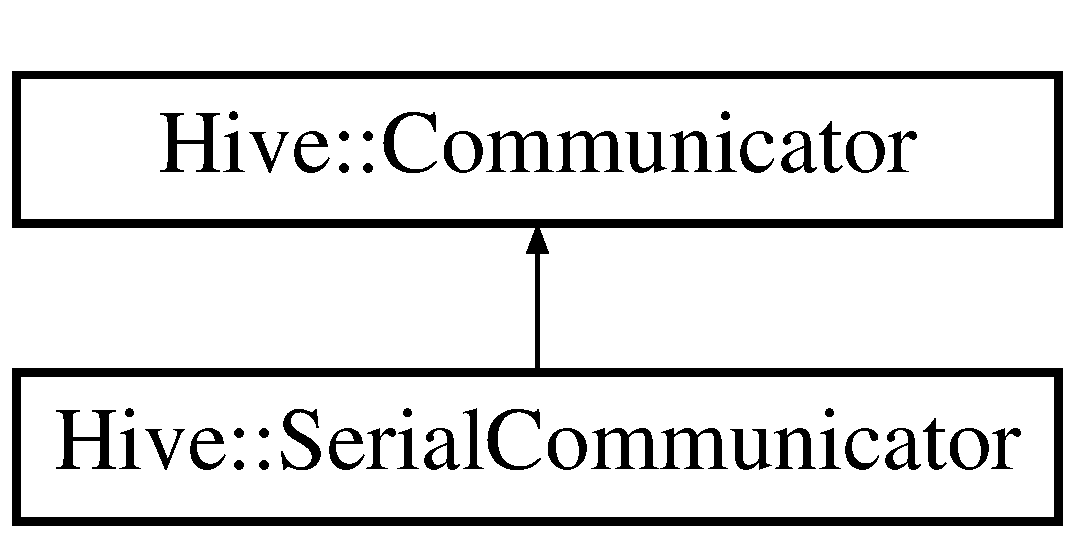
\includegraphics[height=2cm]{classHive_1_1SerialCommunicator}
\end{center}
\end{figure}


\subsection{Detailed Description}
serialcommunicator implements the communicator 

a serial communicator is needed to exchange messages among agent for the case that the entire simulation lives on a single cpu.

\begin{Desc}
\item[{\bf Todo}]\end{Desc}
\begin{Desc}
\item[Author:]garrit jentsch \end{Desc}
\begin{Desc}
\item[Date:]Oct 14, 2009, last edited 10-15-2009 \end{Desc}
\subsection*{Public Member Functions}
\begin{CompactItemize}
\item 
{\bf SerialCommunicator} ()
\begin{CompactList}\small\item\em constructor \item\end{CompactList}\item 
{\bf $\sim$SerialCommunicator} ()
\begin{CompactList}\small\item\em destructor \item\end{CompactList}\item 
void {\bf receiveMessages} ()
\begin{CompactList}\small\item\em method for receiving messages \item\end{CompactList}\item 
void {\bf sendMessage} ({\bf Message} m, int dest)
\item 
void {\bf addAgent} ({\bf Agent} $\ast$a)
\item 
void {\bf setupCommunicationMap} (map$<$ int, {\bf Agent} $\ast$ $>$ \&c)
\item 
void {\bf propogateAgent} (int agentId, double time)
\end{CompactItemize}


\subsection{Constructor \& Destructor Documentation}
\index{Hive::SerialCommunicator@{Hive::SerialCommunicator}!SerialCommunicator@{SerialCommunicator}}
\index{SerialCommunicator@{SerialCommunicator}!Hive::SerialCommunicator@{Hive::SerialCommunicator}}
\subsubsection[SerialCommunicator]{\setlength{\rightskip}{0pt plus 5cm}SerialCommunicator::SerialCommunicator ()}\label{classHive_1_1SerialCommunicator_58aecf7401bc3cb9005d5d7f0f85d5c6}


constructor 

\index{Hive::SerialCommunicator@{Hive::SerialCommunicator}!$\sim$SerialCommunicator@{$\sim$SerialCommunicator}}
\index{$\sim$SerialCommunicator@{$\sim$SerialCommunicator}!Hive::SerialCommunicator@{Hive::SerialCommunicator}}
\subsubsection[$\sim$SerialCommunicator]{\setlength{\rightskip}{0pt plus 5cm}SerialCommunicator::$\sim$SerialCommunicator ()}\label{classHive_1_1SerialCommunicator_df113eec4ac2a38d007616c7231c5033}


destructor 



\subsection{Member Function Documentation}
\index{Hive::SerialCommunicator@{Hive::SerialCommunicator}!receiveMessages@{receiveMessages}}
\index{receiveMessages@{receiveMessages}!Hive::SerialCommunicator@{Hive::SerialCommunicator}}
\subsubsection[receiveMessages]{\setlength{\rightskip}{0pt plus 5cm}void SerialCommunicator::receiveMessages ()\hspace{0.3cm}{\tt  [virtual]}}\label{classHive_1_1SerialCommunicator_020ed57d330b13e4919357dedc72d2f0}


method for receiving messages 



Implements {\bf Hive::Communicator} \doxyref{}{p.}{classHive_1_1Communicator_987b52b99ca4639a198f45c0c74db179}.\index{Hive::SerialCommunicator@{Hive::SerialCommunicator}!sendMessage@{sendMessage}}
\index{sendMessage@{sendMessage}!Hive::SerialCommunicator@{Hive::SerialCommunicator}}
\subsubsection[sendMessage]{\setlength{\rightskip}{0pt plus 5cm}void SerialCommunicator::sendMessage ({\bf Message} {\em m}, \/  int {\em dest})\hspace{0.3cm}{\tt  [virtual]}}\label{classHive_1_1SerialCommunicator_3a50ba8f646e6b63d44707d7bf9e345b}


method for sending messages \begin{Desc}
\item[Parameters:]
\begin{description}
\item[{\em m}]message to be send \item[{\em dest}]identifyer of destination \end{description}
\end{Desc}


Implements {\bf Hive::Communicator} \doxyref{}{p.}{classHive_1_1Communicator_7781e9b8494ed71c91769640bef5e6a3}.\index{Hive::SerialCommunicator@{Hive::SerialCommunicator}!addAgent@{addAgent}}
\index{addAgent@{addAgent}!Hive::SerialCommunicator@{Hive::SerialCommunicator}}
\subsubsection[addAgent]{\setlength{\rightskip}{0pt plus 5cm}void SerialCommunicator::addAgent ({\bf Agent} $\ast$ {\em a})}\label{classHive_1_1SerialCommunicator_1df1993211935f5663a306e5c20e8f9d}


adds an agent to the communication map \begin{Desc}
\item[Parameters:]
\begin{description}
\item[{\em a}]pointer to agent to be added to map \end{description}
\end{Desc}


References Hive::Agent::getAgentId().

Referenced by Dummy::DummyComposer::setupAgentHierarchy().\index{Hive::SerialCommunicator@{Hive::SerialCommunicator}!setupCommunicationMap@{setupCommunicationMap}}
\index{setupCommunicationMap@{setupCommunicationMap}!Hive::SerialCommunicator@{Hive::SerialCommunicator}}
\subsubsection[setupCommunicationMap]{\setlength{\rightskip}{0pt plus 5cm}void SerialCommunicator::setupCommunicationMap (map$<$ int, {\bf Agent} $\ast$ $>$ \& {\em c})}\label{classHive_1_1SerialCommunicator_32689ccc1a3f0e5ae206086240543a7a}


sets up the lookup table \begin{Desc}
\item[Parameters:]
\begin{description}
\item[{\em c}]lookup table \end{description}
\end{Desc}
\index{Hive::SerialCommunicator@{Hive::SerialCommunicator}!propogateAgent@{propogateAgent}}
\index{propogateAgent@{propogateAgent}!Hive::SerialCommunicator@{Hive::SerialCommunicator}}
\subsubsection[propogateAgent]{\setlength{\rightskip}{0pt plus 5cm}void SerialCommunicator::propogateAgent (int {\em agentId}, \/  double {\em time})\hspace{0.3cm}{\tt  [virtual]}}\label{classHive_1_1SerialCommunicator_54021e56fa2936e82c0e9e3d6287cf28}




Implements {\bf Hive::Communicator} \doxyref{}{p.}{classHive_1_1Communicator_8d803da79f8f88bf75a9a306e7676f73}.

The documentation for this class was generated from the following files:\begin{CompactItemize}
\item 
{\bf serialcommunicator.hh}\item 
{\bf serialcommunicator.cpp}\end{CompactItemize}

\section{Hive::Simulator Class Reference}
\label{classHive_1_1Simulator}\index{Hive::Simulator@{Hive::Simulator}}
{\tt \#include $<$simulator.hh$>$}

Inheritance diagram for Hive::Simulator::\begin{figure}[H]
\begin{center}
\leavevmode
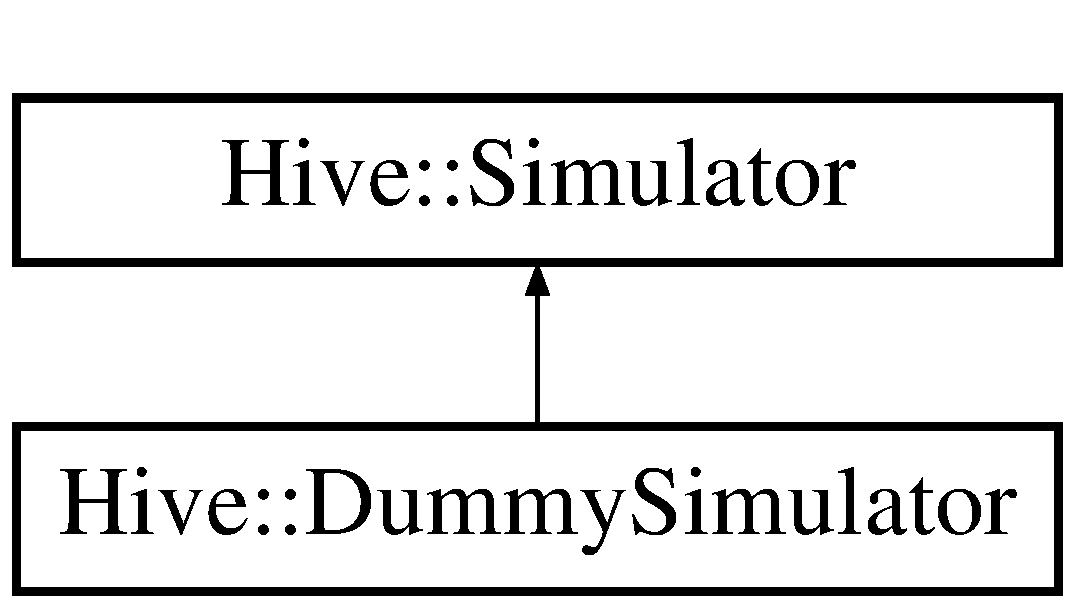
\includegraphics[height=2cm]{classHive_1_1Simulator}
\end{center}
\end{figure}


\subsection{Detailed Description}
simulator class 

a simulator operates on an agent's dataset and propagates it through time. this is an abstract class and the individual simulators have to be derived from this class.

\begin{Desc}
\item[{\bf Todo}]everything\end{Desc}
\begin{Desc}
\item[{\bf Bug}]\end{Desc}
\begin{Desc}
\item[Author:]Garrit Jentsch\end{Desc}
\begin{Desc}
\item[Date:]October 13th, 2009 last edited: 10-14-2009 by Garrit and Michael \end{Desc}
\subsection*{Public Member Functions}
\begin{CompactItemize}
\item 
{\bf Simulator} ()
\begin{CompactList}\small\item\em Constructor. \item\end{CompactList}\item 
virtual {\bf $\sim$Simulator} ()
\begin{CompactList}\small\item\em destructor \item\end{CompactList}\item 
virtual void {\bf step} (double t)=0
\item 
virtual void {\bf prepare} ()=0
\item 
virtual void {\bf synchroniseWithDatabase} ()=0
\end{CompactItemize}
\subsection*{Protected Member Functions}
\begin{CompactItemize}
\item 
virtual void {\bf initialise} ()=0
\end{CompactItemize}
\subsection*{Protected Attributes}
\begin{CompactItemize}
\item 
{\bf Agent} $\ast$ {\bf agent}
\end{CompactItemize}


\subsection{Constructor \& Destructor Documentation}
\index{Hive::Simulator@{Hive::Simulator}!Simulator@{Simulator}}
\index{Simulator@{Simulator}!Hive::Simulator@{Hive::Simulator}}
\subsubsection[Simulator]{\setlength{\rightskip}{0pt plus 5cm}Hive::Simulator::Simulator ()\hspace{0.3cm}{\tt  [inline]}}\label{classHive_1_1Simulator_f21b4a04583a51c8243e20a656f8ae64}


Constructor. 

\index{Hive::Simulator@{Hive::Simulator}!$\sim$Simulator@{$\sim$Simulator}}
\index{$\sim$Simulator@{$\sim$Simulator}!Hive::Simulator@{Hive::Simulator}}
\subsubsection[$\sim$Simulator]{\setlength{\rightskip}{0pt plus 5cm}virtual Hive::Simulator::$\sim$Simulator ()\hspace{0.3cm}{\tt  [inline, virtual]}}\label{classHive_1_1Simulator_8be9b65056772c004ab7e84d4aebe76d}


destructor 



\subsection{Member Function Documentation}
\index{Hive::Simulator@{Hive::Simulator}!step@{step}}
\index{step@{step}!Hive::Simulator@{Hive::Simulator}}
\subsubsection[step]{\setlength{\rightskip}{0pt plus 5cm}virtual void Hive::Simulator::step (double {\em t})\hspace{0.3cm}{\tt  [pure virtual]}}\label{classHive_1_1Simulator_eec111bc06eafdbf4cbc96389c4819d3}


integrate the system for a timestep \begin{Desc}
\item[Parameters:]
\begin{description}
\item[{\em t}]timestep \end{description}
\end{Desc}


Implemented in {\bf Hive::DummySimulator} \doxyref{}{p.}{classHive_1_1DummySimulator_fa489e06187269a63ed18143272d2ef3}.\index{Hive::Simulator@{Hive::Simulator}!prepare@{prepare}}
\index{prepare@{prepare}!Hive::Simulator@{Hive::Simulator}}
\subsubsection[prepare]{\setlength{\rightskip}{0pt plus 5cm}virtual void Hive::Simulator::prepare ()\hspace{0.3cm}{\tt  [pure virtual]}}\label{classHive_1_1Simulator_30d2804d293a3bb84433d83eade34fa3}


prepare simulator for the first time, this will call the connectToDataBase and initialise methods 

Implemented in {\bf Hive::DummySimulator} \doxyref{}{p.}{classHive_1_1DummySimulator_19f750cc2a4d104aca9812e677336d0c}.\index{Hive::Simulator@{Hive::Simulator}!synchroniseWithDatabase@{synchroniseWithDatabase}}
\index{synchroniseWithDatabase@{synchroniseWithDatabase}!Hive::Simulator@{Hive::Simulator}}
\subsubsection[synchroniseWithDatabase]{\setlength{\rightskip}{0pt plus 5cm}virtual void Hive::Simulator::synchroniseWithDatabase ()\hspace{0.3cm}{\tt  [pure virtual]}}\label{classHive_1_1Simulator_b0f2c54ec739d17f1d55a2bbba886793}


update simulator's internal variables before executing the integrate command 

Implemented in {\bf Hive::DummySimulator} \doxyref{}{p.}{classHive_1_1DummySimulator_6ba8f9d234678113768f5c6c400cf208}.\index{Hive::Simulator@{Hive::Simulator}!initialise@{initialise}}
\index{initialise@{initialise}!Hive::Simulator@{Hive::Simulator}}
\subsubsection[initialise]{\setlength{\rightskip}{0pt plus 5cm}virtual void Hive::Simulator::initialise ()\hspace{0.3cm}{\tt  [protected, pure virtual]}}\label{classHive_1_1Simulator_28d5609523dfc40cdc24f8521e032d2c}


initialise simulator's internal variables for the first time 

Implemented in {\bf Hive::DummySimulator} \doxyref{}{p.}{classHive_1_1DummySimulator_45412da18d3233bd8d8b0a9b9fda2361}.

\subsection{Member Data Documentation}
\index{Hive::Simulator@{Hive::Simulator}!agent@{agent}}
\index{agent@{agent}!Hive::Simulator@{Hive::Simulator}}
\subsubsection[agent]{\setlength{\rightskip}{0pt plus 5cm}{\bf Agent}$\ast$ {\bf Hive::Simulator::agent}\hspace{0.3cm}{\tt  [protected]}}\label{classHive_1_1Simulator_080190d6706c82c3b0514b215920d4b1}




Referenced by Hive::DummySimulator::DummySimulator(), Hive::DummySimulator::prepare(), and Hive::DummySimulator::synchroniseWithDatabase().

The documentation for this class was generated from the following file:\begin{CompactItemize}
\item 
{\bf simulator.hh}\end{CompactItemize}

\section{mu::STATIC\_\-ASSERTION\_\-FAILURE$<$ true $>$ Struct Template Reference}
\label{structmu_1_1STATIC__ASSERTION__FAILURE_3_01true_01_4}\index{mu::STATIC\_\-ASSERTION\_\-FAILURE$<$ true $>$@{mu::STATIC\_\-ASSERTION\_\-FAILURE$<$ true $>$}}
{\tt \#include $<$muParserDef.h$>$}

\subsubsection*{template$<$$>$ struct mu::STATIC\_\-ASSERTION\_\-FAILURE$<$ true $>$}



The documentation for this struct was generated from the following file:\begin{CompactItemize}
\item 
{\bf muParserDef.h}\end{CompactItemize}

\section{Hive::System Class Reference}
\label{classHive_1_1System}\index{Hive::System@{Hive::System}}
{\tt \#include $<$system.hh$>$}



\subsection{Detailed Description}
system class 

The system maintains the types of agents that can exist in the simulation. Types of objects allow for the on the fly creation of new agents.

\begin{Desc}
\item[{\bf Todo}]everything, more conceptional work needed. will we have prototypes of agents in here?! it should be a database of types ... whatever ...\end{Desc}
\begin{Desc}
\item[{\bf Bug}]\end{Desc}
\begin{Desc}
\item[Author:]Garrit Jentsch\end{Desc}
\begin{Desc}
\item[Date:]Oct 13th, 2009 last edited 10-14 by Garrit and Michael \end{Desc}
\subsection*{Public Member Functions}
\begin{CompactItemize}
\item 
{\bf System} ()
\begin{CompactList}\small\item\em Constructor. \item\end{CompactList}\item 
virtual {\bf $\sim$System} ()=0
\begin{CompactList}\small\item\em destructor \item\end{CompactList}\item 
int {\bf getSystemType} ()
\end{CompactItemize}
\subsection*{Static Public Attributes}
\begin{CompactItemize}
\item 
static const int {\bf network\_\-free\_\-type} = 0
\begin{CompactList}\small\item\em system type network\_\-free\_\-type \item\end{CompactList}\item 
static const int {\bf kinetic\_\-type} = 1
\begin{CompactList}\small\item\em system type kinetic network \item\end{CompactList}\end{CompactItemize}
\subsection*{Protected Attributes}
\begin{CompactItemize}
\item 
int {\bf system\_\-type}
\begin{CompactList}\small\item\em system type of this system \item\end{CompactList}\end{CompactItemize}


\subsection{Constructor \& Destructor Documentation}
\index{Hive::System@{Hive::System}!System@{System}}
\index{System@{System}!Hive::System@{Hive::System}}
\subsubsection[System]{\setlength{\rightskip}{0pt plus 5cm}Hive::System::System ()}\label{classHive_1_1System_97d30519de767922d0c68e6aea779bf0}


Constructor. 

\index{Hive::System@{Hive::System}!$\sim$System@{$\sim$System}}
\index{$\sim$System@{$\sim$System}!Hive::System@{Hive::System}}
\subsubsection[$\sim$System]{\setlength{\rightskip}{0pt plus 5cm}virtual Hive::System::$\sim$System ()\hspace{0.3cm}{\tt  [pure virtual]}}\label{classHive_1_1System_12d5b725a07e08b97142fae1fae85474}


destructor 



\subsection{Member Function Documentation}
\index{Hive::System@{Hive::System}!getSystemType@{getSystemType}}
\index{getSystemType@{getSystemType}!Hive::System@{Hive::System}}
\subsubsection[getSystemType]{\setlength{\rightskip}{0pt plus 5cm}int Hive::System::getSystemType ()}\label{classHive_1_1System_009aae3c55c070dfc610010b94a1cc08}




\subsection{Member Data Documentation}
\index{Hive::System@{Hive::System}!network\_\-free\_\-type@{network\_\-free\_\-type}}
\index{network\_\-free\_\-type@{network\_\-free\_\-type}!Hive::System@{Hive::System}}
\subsubsection[network\_\-free\_\-type]{\setlength{\rightskip}{0pt plus 5cm}const int {\bf Hive::System::network\_\-free\_\-type} = 0\hspace{0.3cm}{\tt  [static]}}\label{classHive_1_1System_e8fcbcff761ee7459101621d92e07928}


system type network\_\-free\_\-type 

\index{Hive::System@{Hive::System}!kinetic\_\-type@{kinetic\_\-type}}
\index{kinetic\_\-type@{kinetic\_\-type}!Hive::System@{Hive::System}}
\subsubsection[kinetic\_\-type]{\setlength{\rightskip}{0pt plus 5cm}const int {\bf Hive::System::kinetic\_\-type} = 1\hspace{0.3cm}{\tt  [static]}}\label{classHive_1_1System_e792ebbacd05e3f5cc1dfa725e7cb0b7}


system type kinetic network 

\index{Hive::System@{Hive::System}!system\_\-type@{system\_\-type}}
\index{system\_\-type@{system\_\-type}!Hive::System@{Hive::System}}
\subsubsection[system\_\-type]{\setlength{\rightskip}{0pt plus 5cm}int {\bf Hive::System::system\_\-type}\hspace{0.3cm}{\tt  [protected]}}\label{classHive_1_1System_203a63d9870f21f74dfe53a73bd797c4}


system type of this system 



The documentation for this class was generated from the following file:\begin{CompactItemize}
\item 
{\bf system.hh}\end{CompactItemize}

\section{TiXmlAttribute Class Reference}
\label{classTiXmlAttribute}\index{TiXmlAttribute@{TiXmlAttribute}}
{\tt \#include $<$tinyxml.h$>$}

Inheritance diagram for TiXmlAttribute::\begin{figure}[H]
\begin{center}
\leavevmode
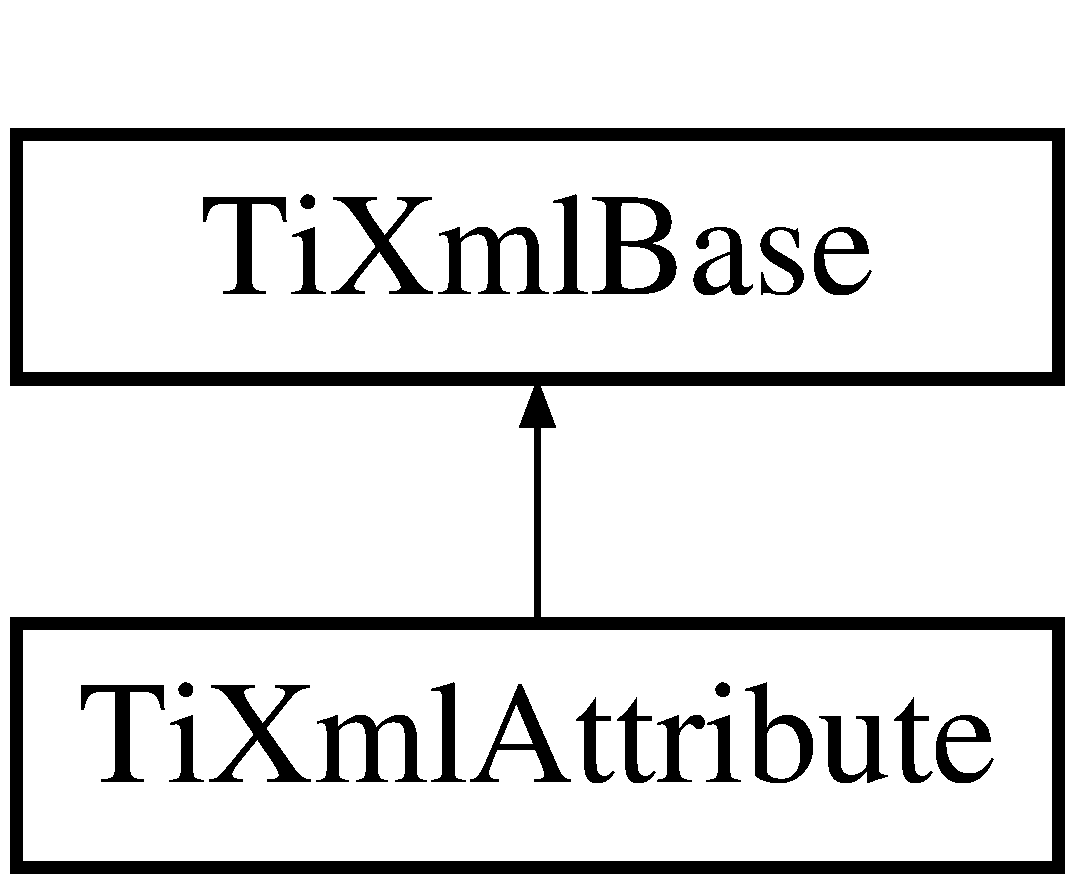
\includegraphics[height=2cm]{classTiXmlAttribute}
\end{center}
\end{figure}


\subsection{Detailed Description}
An attribute is a name-value pair. Elements have an arbitrary number of attributes, each with a unique name.

\begin{Desc}
\item[Note:]The attributes are not TiXmlNodes, since they are not part of the tinyXML document object model. There are other suggested ways to look at this problem. \end{Desc}
\subsection*{Public Member Functions}
\begin{CompactItemize}
\item 
{\bf TiXmlAttribute} ()
\begin{CompactList}\small\item\em Construct an empty attribute. \item\end{CompactList}\item 
{\bf TiXmlAttribute} (const char $\ast$\_\-name, const char $\ast$\_\-value)
\begin{CompactList}\small\item\em Construct an attribute with a name and value. \item\end{CompactList}\item 
const char $\ast$ {\bf Name} () const 
\begin{CompactList}\small\item\em Return the name of this attribute. \item\end{CompactList}\item 
const char $\ast$ {\bf Value} () const 
\begin{CompactList}\small\item\em Return the value of this attribute. \item\end{CompactList}\item 
int {\bf IntValue} () const 
\begin{CompactList}\small\item\em Return the value of this attribute, converted to an integer. \item\end{CompactList}\item 
double {\bf DoubleValue} () const 
\begin{CompactList}\small\item\em Return the value of this attribute, converted to a double. \item\end{CompactList}\item 
const TIXML\_\-STRING \& {\bf NameTStr} () const 
\item 
int {\bf QueryIntValue} (int $\ast$\_\-value) const 
\item 
int {\bf QueryDoubleValue} (double $\ast$\_\-value) const 
\begin{CompactList}\small\item\em QueryDoubleValue examines the value string. See \doxyref{QueryIntValue()}{p.}{classTiXmlAttribute_d6c93088ee21af41a107931223339344}. \item\end{CompactList}\item 
void {\bf SetName} (const char $\ast$\_\-name)
\begin{CompactList}\small\item\em Set the name of this attribute. \item\end{CompactList}\item 
void {\bf SetValue} (const char $\ast$\_\-value)
\begin{CompactList}\small\item\em Set the value. \item\end{CompactList}\item 
void {\bf SetIntValue} (int \_\-value)
\begin{CompactList}\small\item\em Set the value from an integer. \item\end{CompactList}\item 
void {\bf SetDoubleValue} (double \_\-value)
\begin{CompactList}\small\item\em Set the value from a double. \item\end{CompactList}\item 
const {\bf TiXmlAttribute} $\ast$ {\bf Next} () const 
\begin{CompactList}\small\item\em Get the next sibling attribute in the DOM. Returns null at end. \item\end{CompactList}\item 
{\bf TiXmlAttribute} $\ast$ {\bf Next} ()
\item 
const {\bf TiXmlAttribute} $\ast$ {\bf Previous} () const 
\begin{CompactList}\small\item\em Get the previous sibling attribute in the DOM. Returns null at beginning. \item\end{CompactList}\item 
{\bf TiXmlAttribute} $\ast$ {\bf Previous} ()
\item 
bool {\bf operator==} (const {\bf TiXmlAttribute} \&rhs) const 
\item 
bool {\bf operator$<$} (const {\bf TiXmlAttribute} \&rhs) const 
\item 
bool {\bf operator$>$} (const {\bf TiXmlAttribute} \&rhs) const 
\item 
virtual const char $\ast$ {\bf Parse} (const char $\ast$p, {\bf TiXmlParsingData} $\ast$data, {\bf TiXmlEncoding} encoding)
\item 
virtual void {\bf Print} (FILE $\ast$cfile, int depth) const 
\item 
void {\bf Print} (FILE $\ast$cfile, int depth, TIXML\_\-STRING $\ast$str) const 
\item 
void {\bf SetDocument} ({\bf TiXmlDocument} $\ast$doc)
\end{CompactItemize}
\subsection*{Friends}
\begin{CompactItemize}
\item 
class {\bf TiXmlAttributeSet}
\end{CompactItemize}


\subsection{Constructor \& Destructor Documentation}
\index{TiXmlAttribute@{TiXmlAttribute}!TiXmlAttribute@{TiXmlAttribute}}
\index{TiXmlAttribute@{TiXmlAttribute}!TiXmlAttribute@{TiXmlAttribute}}
\subsubsection[TiXmlAttribute]{\setlength{\rightskip}{0pt plus 5cm}TiXmlAttribute::TiXmlAttribute ()\hspace{0.3cm}{\tt  [inline]}}\label{classTiXmlAttribute_9cfa3c8179873fd485d83003b114f8e1}


Construct an empty attribute. 

\index{TiXmlAttribute@{TiXmlAttribute}!TiXmlAttribute@{TiXmlAttribute}}
\index{TiXmlAttribute@{TiXmlAttribute}!TiXmlAttribute@{TiXmlAttribute}}
\subsubsection[TiXmlAttribute]{\setlength{\rightskip}{0pt plus 5cm}TiXmlAttribute::TiXmlAttribute (const char $\ast$ {\em \_\-name}, \/  const char $\ast$ {\em \_\-value})\hspace{0.3cm}{\tt  [inline]}}\label{classTiXmlAttribute_759d0b76fb8fcf765ecab243bc14f05e}


Construct an attribute with a name and value. 



\subsection{Member Function Documentation}
\index{TiXmlAttribute@{TiXmlAttribute}!Name@{Name}}
\index{Name@{Name}!TiXmlAttribute@{TiXmlAttribute}}
\subsubsection[Name]{\setlength{\rightskip}{0pt plus 5cm}const char$\ast$ TiXmlAttribute::Name () const\hspace{0.3cm}{\tt  [inline]}}\label{classTiXmlAttribute_298a57287d305904ba6bd96ae6f78d3d}


Return the name of this attribute. 



Referenced by TiXmlAttributeSet::Add(), TiXmlElement::CopyTo(), and TiXmlElement::Parse().\index{TiXmlAttribute@{TiXmlAttribute}!Value@{Value}}
\index{Value@{Value}!TiXmlAttribute@{TiXmlAttribute}}
\subsubsection[Value]{\setlength{\rightskip}{0pt plus 5cm}const char$\ast$ TiXmlAttribute::Value () const\hspace{0.3cm}{\tt  [inline]}}\label{classTiXmlAttribute_0f874490eac8ca00ee0070765d0e97e3}


Return the value of this attribute. 



Referenced by TiXmlElement::Attribute(), TiXmlElement::CopyTo(), TiXmlDeclaration::Parse(), and TiXmlElement::Parse().\index{TiXmlAttribute@{TiXmlAttribute}!IntValue@{IntValue}}
\index{IntValue@{IntValue}!TiXmlAttribute@{TiXmlAttribute}}
\subsubsection[IntValue]{\setlength{\rightskip}{0pt plus 5cm}int TiXmlAttribute::IntValue () const}\label{classTiXmlAttribute_a1a20ad59dc7e89a0ab265396360d50f}


Return the value of this attribute, converted to an integer. 

\index{TiXmlAttribute@{TiXmlAttribute}!DoubleValue@{DoubleValue}}
\index{DoubleValue@{DoubleValue}!TiXmlAttribute@{TiXmlAttribute}}
\subsubsection[DoubleValue]{\setlength{\rightskip}{0pt plus 5cm}double TiXmlAttribute::DoubleValue () const}\label{classTiXmlAttribute_2880ddef53fc7522c99535273954d230}


Return the value of this attribute, converted to a double. 

\index{TiXmlAttribute@{TiXmlAttribute}!NameTStr@{NameTStr}}
\index{NameTStr@{NameTStr}!TiXmlAttribute@{TiXmlAttribute}}
\subsubsection[NameTStr]{\setlength{\rightskip}{0pt plus 5cm}const TIXML\_\-STRING\& TiXmlAttribute::NameTStr () const\hspace{0.3cm}{\tt  [inline]}}\label{classTiXmlAttribute_64cee17bceb8232eb0736d26dd082d79}




Referenced by TiXmlElement::Parse().\index{TiXmlAttribute@{TiXmlAttribute}!QueryIntValue@{QueryIntValue}}
\index{QueryIntValue@{QueryIntValue}!TiXmlAttribute@{TiXmlAttribute}}
\subsubsection[QueryIntValue]{\setlength{\rightskip}{0pt plus 5cm}int TiXmlAttribute::QueryIntValue (int $\ast$ {\em \_\-value}) const}\label{classTiXmlAttribute_d6c93088ee21af41a107931223339344}


QueryIntValue examines the value string. It is an alternative to the \doxyref{IntValue()}{p.}{classTiXmlAttribute_a1a20ad59dc7e89a0ab265396360d50f} method with richer error checking. If the value is an integer, it is stored in 'value' and the call returns TIXML\_\-SUCCESS. If it is not an integer, it returns TIXML\_\-WRONG\_\-TYPE.

A specialized but useful call. Note that for success it returns 0, which is the opposite of almost all other TinyXml calls. 

References TIXML\_\-SSCANF, TIXML\_\-SUCCESS, and TIXML\_\-WRONG\_\-TYPE.

Referenced by TiXmlElement::QueryIntAttribute().\index{TiXmlAttribute@{TiXmlAttribute}!QueryDoubleValue@{QueryDoubleValue}}
\index{QueryDoubleValue@{QueryDoubleValue}!TiXmlAttribute@{TiXmlAttribute}}
\subsubsection[QueryDoubleValue]{\setlength{\rightskip}{0pt plus 5cm}int TiXmlAttribute::QueryDoubleValue (double $\ast$ {\em \_\-value}) const}\label{classTiXmlAttribute_c87b2a8489906a5d7aa2875f20be3513}


QueryDoubleValue examines the value string. See \doxyref{QueryIntValue()}{p.}{classTiXmlAttribute_d6c93088ee21af41a107931223339344}. 



References TIXML\_\-SSCANF, TIXML\_\-SUCCESS, and TIXML\_\-WRONG\_\-TYPE.

Referenced by TiXmlElement::QueryDoubleAttribute().\index{TiXmlAttribute@{TiXmlAttribute}!SetName@{SetName}}
\index{SetName@{SetName}!TiXmlAttribute@{TiXmlAttribute}}
\subsubsection[SetName]{\setlength{\rightskip}{0pt plus 5cm}void TiXmlAttribute::SetName (const char $\ast$ {\em \_\-name})\hspace{0.3cm}{\tt  [inline]}}\label{classTiXmlAttribute_b7fa3d21ff8d7c5764cf9af15b667a99}


Set the name of this attribute. 

\index{TiXmlAttribute@{TiXmlAttribute}!SetValue@{SetValue}}
\index{SetValue@{SetValue}!TiXmlAttribute@{TiXmlAttribute}}
\subsubsection[SetValue]{\setlength{\rightskip}{0pt plus 5cm}void TiXmlAttribute::SetValue (const char $\ast$ {\em \_\-value})\hspace{0.3cm}{\tt  [inline]}}\label{classTiXmlAttribute_2dae44178f668b3cb48101be4f2236a0}


Set the value. 



Referenced by TiXmlElement::Parse(), TiXmlElement::SetAttribute(), SetDoubleValue(), and SetIntValue().\index{TiXmlAttribute@{TiXmlAttribute}!SetIntValue@{SetIntValue}}
\index{SetIntValue@{SetIntValue}!TiXmlAttribute@{TiXmlAttribute}}
\subsubsection[SetIntValue]{\setlength{\rightskip}{0pt plus 5cm}void TiXmlAttribute::SetIntValue (int {\em \_\-value})}\label{classTiXmlAttribute_7e065df640116a62ea4f4b7da5449cc8}


Set the value from an integer. 



References SetValue().\index{TiXmlAttribute@{TiXmlAttribute}!SetDoubleValue@{SetDoubleValue}}
\index{SetDoubleValue@{SetDoubleValue}!TiXmlAttribute@{TiXmlAttribute}}
\subsubsection[SetDoubleValue]{\setlength{\rightskip}{0pt plus 5cm}void TiXmlAttribute::SetDoubleValue (double {\em \_\-value})}\label{classTiXmlAttribute_0316da31373496c4368ad549bf711394}


Set the value from a double. 



References SetValue().\index{TiXmlAttribute@{TiXmlAttribute}!Next@{Next}}
\index{Next@{Next}!TiXmlAttribute@{TiXmlAttribute}}
\subsubsection[Next]{\setlength{\rightskip}{0pt plus 5cm}const {\bf TiXmlAttribute} $\ast$ TiXmlAttribute::Next () const}\label{classTiXmlAttribute_776478980776a024f7c2846eec640f65}


Get the next sibling attribute in the DOM. Returns null at end. 



References name, and value.

Referenced by TiXmlElement::CopyTo(), TiXmlElement::Print(), and TiXmlPrinter::VisitEnter().\index{TiXmlAttribute@{TiXmlAttribute}!Next@{Next}}
\index{Next@{Next}!TiXmlAttribute@{TiXmlAttribute}}
\subsubsection[Next]{\setlength{\rightskip}{0pt plus 5cm}{\bf TiXmlAttribute}$\ast$ TiXmlAttribute::Next ()\hspace{0.3cm}{\tt  [inline]}}\label{classTiXmlAttribute_138320aa7793b148ba7e5bd0a0ea4db6}


\index{TiXmlAttribute@{TiXmlAttribute}!Previous@{Previous}}
\index{Previous@{Previous}!TiXmlAttribute@{TiXmlAttribute}}
\subsubsection[Previous]{\setlength{\rightskip}{0pt plus 5cm}const {\bf TiXmlAttribute} $\ast$ TiXmlAttribute::Previous () const}\label{classTiXmlAttribute_54a5f8730c7b02b9a41b74e12e27fe86}


Get the previous sibling attribute in the DOM. Returns null at beginning. 



References name, and value.\index{TiXmlAttribute@{TiXmlAttribute}!Previous@{Previous}}
\index{Previous@{Previous}!TiXmlAttribute@{TiXmlAttribute}}
\subsubsection[Previous]{\setlength{\rightskip}{0pt plus 5cm}{\bf TiXmlAttribute}$\ast$ TiXmlAttribute::Previous ()\hspace{0.3cm}{\tt  [inline]}}\label{classTiXmlAttribute_e4dabc932cba945ed1e92fec5f121193}


\index{TiXmlAttribute@{TiXmlAttribute}!operator==@{operator==}}
\index{operator==@{operator==}!TiXmlAttribute@{TiXmlAttribute}}
\subsubsection[operator==]{\setlength{\rightskip}{0pt plus 5cm}bool TiXmlAttribute::operator== (const {\bf TiXmlAttribute} \& {\em rhs}) const\hspace{0.3cm}{\tt  [inline]}}\label{classTiXmlAttribute_e48c2a65b520d453914ce4e845d607cf}




References name.\index{TiXmlAttribute@{TiXmlAttribute}!operator$<$@{operator$<$}}
\index{operator$<$@{operator$<$}!TiXmlAttribute@{TiXmlAttribute}}
\subsubsection[operator$<$]{\setlength{\rightskip}{0pt plus 5cm}bool TiXmlAttribute::operator$<$ (const {\bf TiXmlAttribute} \& {\em rhs}) const\hspace{0.3cm}{\tt  [inline]}}\label{classTiXmlAttribute_db8b6f2cad5948e73e383182e7ce10de}




References name.\index{TiXmlAttribute@{TiXmlAttribute}!operator$>$@{operator$>$}}
\index{operator$>$@{operator$>$}!TiXmlAttribute@{TiXmlAttribute}}
\subsubsection[operator$>$]{\setlength{\rightskip}{0pt plus 5cm}bool TiXmlAttribute::operator$>$ (const {\bf TiXmlAttribute} \& {\em rhs}) const\hspace{0.3cm}{\tt  [inline]}}\label{classTiXmlAttribute_867562769ef9778c1690cd373246b05b}




References name.\index{TiXmlAttribute@{TiXmlAttribute}!Parse@{Parse}}
\index{Parse@{Parse}!TiXmlAttribute@{TiXmlAttribute}}
\subsubsection[Parse]{\setlength{\rightskip}{0pt plus 5cm}const char $\ast$ TiXmlAttribute::Parse (const char $\ast$ {\em p}, \/  {\bf TiXmlParsingData} $\ast$ {\em data}, \/  {\bf TiXmlEncoding} {\em encoding})\hspace{0.3cm}{\tt  [virtual]}}\label{classTiXmlAttribute_d62774421b814894b995af3b5d231dda}




Implements {\bf TiXmlBase} \doxyref{}{p.}{classTiXmlBase_00e4edb0219d00a1379c856e5a1d2025}.

References TiXmlParsingData::Cursor(), TiXmlBase::IsWhiteSpace(), TiXmlBase::location, TiXmlBase::ReadName(), TiXmlBase::ReadText(), TiXmlDocument::SetError(), TiXmlBase::SkipWhiteSpace(), TiXmlParsingData::Stamp(), TiXmlBase::TIXML\_\-ERROR\_\-READING\_\-ATTRIBUTES, and TiXmlNode::value.

Referenced by TiXmlDeclaration::Parse(), and TiXmlElement::Parse().\index{TiXmlAttribute@{TiXmlAttribute}!Print@{Print}}
\index{Print@{Print}!TiXmlAttribute@{TiXmlAttribute}}
\subsubsection[Print]{\setlength{\rightskip}{0pt plus 5cm}virtual void TiXmlAttribute::Print (FILE $\ast$ {\em cfile}, \/  int {\em depth}) const\hspace{0.3cm}{\tt  [inline, virtual]}}\label{classTiXmlAttribute_cc04956c1d5c4c31fe74f7a7528d109a}


All TinyXml classes can print themselves to a filestream or the string class (\doxyref{TiXmlString}{p.}{classTiXmlString} in non-STL mode, std::string in STL mode.) Either or both cfile and str can be null.

This is a formatted print, and will insert tabs and newlines.

(For an unformatted stream, use the $<$$<$ operator.) 

Implements {\bf TiXmlBase} \doxyref{}{p.}{classTiXmlBase_0de56b3f2ef14c65091a3b916437b512}.

Referenced by TiXmlPrinter::VisitEnter().\index{TiXmlAttribute@{TiXmlAttribute}!Print@{Print}}
\index{Print@{Print}!TiXmlAttribute@{TiXmlAttribute}}
\subsubsection[Print]{\setlength{\rightskip}{0pt plus 5cm}void TiXmlAttribute::Print (FILE $\ast$ {\em cfile}, \/  int {\em depth}, \/  TIXML\_\-STRING $\ast$ {\em str}) const}\label{classTiXmlAttribute_19e6b6862a80b188571c47947e88d030}




References TiXmlBase::EncodeString(), and TIXML\_\-STRING.\index{TiXmlAttribute@{TiXmlAttribute}!SetDocument@{SetDocument}}
\index{SetDocument@{SetDocument}!TiXmlAttribute@{TiXmlAttribute}}
\subsubsection[SetDocument]{\setlength{\rightskip}{0pt plus 5cm}void TiXmlAttribute::SetDocument ({\bf TiXmlDocument} $\ast$ {\em doc})\hspace{0.3cm}{\tt  [inline]}}\label{classTiXmlAttribute_c12a94d4548302afb12f488ba101f7d1}




Referenced by TiXmlElement::Parse().

\subsection{Friends And Related Function Documentation}
\index{TiXmlAttribute@{TiXmlAttribute}!TiXmlAttributeSet@{TiXmlAttributeSet}}
\index{TiXmlAttributeSet@{TiXmlAttributeSet}!TiXmlAttribute@{TiXmlAttribute}}
\subsubsection[TiXmlAttributeSet]{\setlength{\rightskip}{0pt plus 5cm}friend class {\bf TiXmlAttributeSet}\hspace{0.3cm}{\tt  [friend]}}\label{classTiXmlAttribute_35a7b7f89f708527677d5078d41ce0bf}




The documentation for this class was generated from the following files:\begin{CompactItemize}
\item 
{\bf tinyxml.h}\item 
{\bf tinyxml.cpp}\item 
{\bf tinyxmlparser.cpp}\end{CompactItemize}

\section{TiXmlAttributeSet Class Reference}
\label{classTiXmlAttributeSet}\index{TiXmlAttributeSet@{TiXmlAttributeSet}}
{\tt \#include $<$tinyxml.h$>$}



\subsection{Detailed Description}
A class used to manage a group of attributes. It is only used internally, both by the ELEMENT and the DECLARATION.

The set can be changed transparent to the Element and Declaration classes that use it, but NOT transparent to the Attribute which has to implement a next() and previous() method. Which makes it a bit problematic and prevents the use of STL.

This version is implemented with circular lists because:\begin{itemize}
\item I like circular lists\item it demonstrates some independence from the (typical) doubly linked list. \end{itemize}
\subsection*{Public Member Functions}
\begin{CompactItemize}
\item 
{\bf TiXmlAttributeSet} ()
\item 
{\bf $\sim$TiXmlAttributeSet} ()
\item 
void {\bf Add} ({\bf TiXmlAttribute} $\ast$attribute)
\item 
void {\bf Remove} ({\bf TiXmlAttribute} $\ast$attribute)
\item 
const {\bf TiXmlAttribute} $\ast$ {\bf First} () const 
\item 
{\bf TiXmlAttribute} $\ast$ {\bf First} ()
\item 
const {\bf TiXmlAttribute} $\ast$ {\bf Last} () const 
\item 
{\bf TiXmlAttribute} $\ast$ {\bf Last} ()
\item 
const {\bf TiXmlAttribute} $\ast$ {\bf Find} (const char $\ast$\_\-name) const 
\item 
{\bf TiXmlAttribute} $\ast$ {\bf Find} (const char $\ast$\_\-name)
\end{CompactItemize}


\subsection{Constructor \& Destructor Documentation}
\index{TiXmlAttributeSet@{TiXmlAttributeSet}!TiXmlAttributeSet@{TiXmlAttributeSet}}
\index{TiXmlAttributeSet@{TiXmlAttributeSet}!TiXmlAttributeSet@{TiXmlAttributeSet}}
\subsubsection[TiXmlAttributeSet]{\setlength{\rightskip}{0pt plus 5cm}TiXmlAttributeSet::TiXmlAttributeSet ()}\label{classTiXmlAttributeSet_253c33b657cc85a07f7f060b02146c35}




References TiXmlAttribute::next, and TiXmlAttribute::prev.\index{TiXmlAttributeSet@{TiXmlAttributeSet}!$\sim$TiXmlAttributeSet@{$\sim$TiXmlAttributeSet}}
\index{$\sim$TiXmlAttributeSet@{$\sim$TiXmlAttributeSet}!TiXmlAttributeSet@{TiXmlAttributeSet}}
\subsubsection[$\sim$TiXmlAttributeSet]{\setlength{\rightskip}{0pt plus 5cm}TiXmlAttributeSet::$\sim$TiXmlAttributeSet ()}\label{classTiXmlAttributeSet_dd463905dff96142a29fe16a01ecf28f}




References TiXmlAttribute::next, and TiXmlAttribute::prev.

\subsection{Member Function Documentation}
\index{TiXmlAttributeSet@{TiXmlAttributeSet}!Add@{Add}}
\index{Add@{Add}!TiXmlAttributeSet@{TiXmlAttributeSet}}
\subsubsection[Add]{\setlength{\rightskip}{0pt plus 5cm}void TiXmlAttributeSet::Add ({\bf TiXmlAttribute} $\ast$ {\em attribute})}\label{classTiXmlAttributeSet_745e50ddaae3bee93e4589321e0b9c1a}




References Find(), TiXmlAttribute::Name(), TiXmlAttribute::next, TiXmlAttribute::prev, and TIXML\_\-STRING.

Referenced by TiXmlElement::Parse(), and TiXmlElement::SetAttribute().\index{TiXmlAttributeSet@{TiXmlAttributeSet}!Remove@{Remove}}
\index{Remove@{Remove}!TiXmlAttributeSet@{TiXmlAttributeSet}}
\subsubsection[Remove]{\setlength{\rightskip}{0pt plus 5cm}void TiXmlAttributeSet::Remove ({\bf TiXmlAttribute} $\ast$ {\em attribute})}\label{classTiXmlAttributeSet_924a73d071f2573f9060f0be57879c57}




References TiXmlAttribute::next, and TiXmlAttribute::prev.

Referenced by TiXmlElement::ClearThis(), and TiXmlElement::RemoveAttribute().\index{TiXmlAttributeSet@{TiXmlAttributeSet}!First@{First}}
\index{First@{First}!TiXmlAttributeSet@{TiXmlAttributeSet}}
\subsubsection[First]{\setlength{\rightskip}{0pt plus 5cm}const {\bf TiXmlAttribute}$\ast$ TiXmlAttributeSet::First () const\hspace{0.3cm}{\tt  [inline]}}\label{classTiXmlAttributeSet_e0636e88cedd4b09d61c451860f68598}




References TiXmlAttribute::next.

Referenced by TiXmlElement::Accept(), TiXmlElement::ClearThis(), TiXmlElement::CopyTo(), TiXmlElement::FirstAttribute(), and TiXmlElement::Print().\index{TiXmlAttributeSet@{TiXmlAttributeSet}!First@{First}}
\index{First@{First}!TiXmlAttributeSet@{TiXmlAttributeSet}}
\subsubsection[First]{\setlength{\rightskip}{0pt plus 5cm}{\bf TiXmlAttribute}$\ast$ TiXmlAttributeSet::First ()\hspace{0.3cm}{\tt  [inline]}}\label{classTiXmlAttributeSet_99703bb08ca2aece2d7ef835de339ba0}




References TiXmlAttribute::next.\index{TiXmlAttributeSet@{TiXmlAttributeSet}!Last@{Last}}
\index{Last@{Last}!TiXmlAttributeSet@{TiXmlAttributeSet}}
\subsubsection[Last]{\setlength{\rightskip}{0pt plus 5cm}const {\bf TiXmlAttribute}$\ast$ TiXmlAttributeSet::Last () const\hspace{0.3cm}{\tt  [inline]}}\label{classTiXmlAttributeSet_7b3f3ccf39a97bc25539d3fcc540296a}




References TiXmlAttribute::prev.

Referenced by TiXmlElement::LastAttribute().\index{TiXmlAttributeSet@{TiXmlAttributeSet}!Last@{Last}}
\index{Last@{Last}!TiXmlAttributeSet@{TiXmlAttributeSet}}
\subsubsection[Last]{\setlength{\rightskip}{0pt plus 5cm}{\bf TiXmlAttribute}$\ast$ TiXmlAttributeSet::Last ()\hspace{0.3cm}{\tt  [inline]}}\label{classTiXmlAttributeSet_b4c4edfb2d74f6ea31aae096743bd6e0}




References TiXmlAttribute::prev.\index{TiXmlAttributeSet@{TiXmlAttributeSet}!Find@{Find}}
\index{Find@{Find}!TiXmlAttributeSet@{TiXmlAttributeSet}}
\subsubsection[Find]{\setlength{\rightskip}{0pt plus 5cm}const {\bf TiXmlAttribute} $\ast$ TiXmlAttributeSet::Find (const char $\ast$ {\em \_\-name}) const}\label{classTiXmlAttributeSet_acbbc5e1a1c987e72815430e89fcb58b}




References TiXmlNode::next, and TiXmlAttribute::next.

Referenced by Add(), TiXmlElement::Attribute(), TiXmlElement::Parse(), TiXmlElement::QueryDoubleAttribute(), TiXmlElement::QueryIntAttribute(), TiXmlElement::RemoveAttribute(), and TiXmlElement::SetAttribute().\index{TiXmlAttributeSet@{TiXmlAttributeSet}!Find@{Find}}
\index{Find@{Find}!TiXmlAttributeSet@{TiXmlAttributeSet}}
\subsubsection[Find]{\setlength{\rightskip}{0pt plus 5cm}{\bf TiXmlAttribute}$\ast$ TiXmlAttributeSet::Find (const char $\ast$ {\em \_\-name})\hspace{0.3cm}{\tt  [inline]}}\label{classTiXmlAttributeSet_2f210bed54c832adf1683c44c35727b9}




The documentation for this class was generated from the following files:\begin{CompactItemize}
\item 
{\bf tinyxml.h}\item 
{\bf tinyxml.cpp}\end{CompactItemize}

\section{TiXmlBase Class Reference}
\label{classTiXmlBase}\index{TiXmlBase@{TiXmlBase}}
{\tt \#include $<$tinyxml.h$>$}

Inheritance diagram for TiXmlBase::\begin{figure}[H]
\begin{center}
\leavevmode
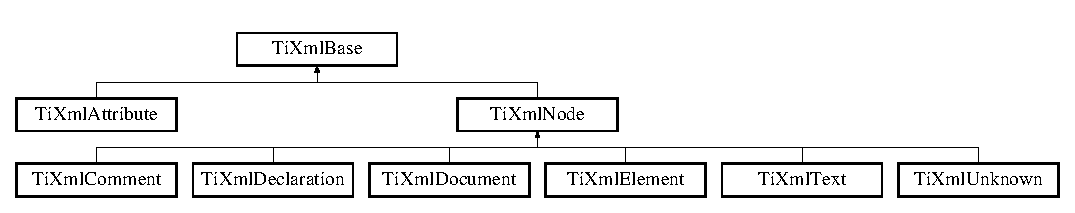
\includegraphics[height=2.41379cm]{classTiXmlBase}
\end{center}
\end{figure}


\subsection{Detailed Description}
\doxyref{TiXmlBase}{p.}{classTiXmlBase} is a base class for every class in TinyXml. It does little except to establish that TinyXml classes can be printed and provide some utility functions.

In XML, the document and elements can contain other elements and other types of nodes.



\footnotesize\begin{verbatim}
	A Document can contain:	Element	(container or leaf)
							Comment (leaf)
							Unknown (leaf)
							Declaration( leaf )

	An Element can contain:	Element (container or leaf)
							Text	(leaf)
							Attributes (not on tree)
							Comment (leaf)
							Unknown (leaf)

	A Decleration contains: Attributes (not on tree)
	\end{verbatim}
\normalsize
 \subsection*{Public Types}
\begin{CompactItemize}
\item 
enum \{ \par
{\bf TIXML\_\-NO\_\-ERROR} =  0, 
{\bf TIXML\_\-ERROR}, 
{\bf TIXML\_\-ERROR\_\-OPENING\_\-FILE}, 
{\bf TIXML\_\-ERROR\_\-OUT\_\-OF\_\-MEMORY}, 
\par
{\bf TIXML\_\-ERROR\_\-PARSING\_\-ELEMENT}, 
{\bf TIXML\_\-ERROR\_\-FAILED\_\-TO\_\-READ\_\-ELEMENT\_\-NAME}, 
{\bf TIXML\_\-ERROR\_\-READING\_\-ELEMENT\_\-VALUE}, 
{\bf TIXML\_\-ERROR\_\-READING\_\-ATTRIBUTES}, 
\par
{\bf TIXML\_\-ERROR\_\-PARSING\_\-EMPTY}, 
{\bf TIXML\_\-ERROR\_\-READING\_\-END\_\-TAG}, 
{\bf TIXML\_\-ERROR\_\-PARSING\_\-UNKNOWN}, 
{\bf TIXML\_\-ERROR\_\-PARSING\_\-COMMENT}, 
\par
{\bf TIXML\_\-ERROR\_\-PARSING\_\-DECLARATION}, 
{\bf TIXML\_\-ERROR\_\-DOCUMENT\_\-EMPTY}, 
{\bf TIXML\_\-ERROR\_\-EMBEDDED\_\-NULL}, 
{\bf TIXML\_\-ERROR\_\-PARSING\_\-CDATA}, 
\par
{\bf TIXML\_\-ERROR\_\-DOCUMENT\_\-TOP\_\-ONLY}, 
{\bf TIXML\_\-ERROR\_\-STRING\_\-COUNT}
 \}
\end{CompactItemize}
\subsection*{Public Member Functions}
\begin{CompactItemize}
\item 
{\bf TiXmlBase} ()
\item 
virtual {\bf $\sim$TiXmlBase} ()
\item 
virtual void {\bf Print} (FILE $\ast$cfile, int depth) const =0
\item 
int {\bf Row} () const 
\item 
int {\bf Column} () const 
\begin{CompactList}\small\item\em See \doxyref{Row()}{p.}{classTiXmlBase_024bceb070188df92c2a8d8852dd0853}. \item\end{CompactList}\item 
void {\bf SetUserData} (void $\ast$user)
\begin{CompactList}\small\item\em Set a pointer to arbitrary user data. \item\end{CompactList}\item 
void $\ast$ {\bf GetUserData} ()
\begin{CompactList}\small\item\em Get a pointer to arbitrary user data. \item\end{CompactList}\item 
const void $\ast$ {\bf GetUserData} () const 
\begin{CompactList}\small\item\em Get a pointer to arbitrary user data. \item\end{CompactList}\item 
virtual const char $\ast$ {\bf Parse} (const char $\ast$p, {\bf TiXmlParsingData} $\ast$data, {\bf TiXmlEncoding} encoding)=0
\end{CompactItemize}
\subsection*{Static Public Member Functions}
\begin{CompactItemize}
\item 
static void {\bf SetCondenseWhiteSpace} (bool condense)
\item 
static bool {\bf IsWhiteSpaceCondensed} ()
\begin{CompactList}\small\item\em Return the current white space setting. \item\end{CompactList}\item 
static void {\bf EncodeString} (const TIXML\_\-STRING \&str, TIXML\_\-STRING $\ast$out)
\end{CompactItemize}
\subsection*{Static Public Attributes}
\begin{CompactItemize}
\item 
static const int {\bf utf8ByteTable} [256]
\end{CompactItemize}
\subsection*{Static Protected Member Functions}
\begin{CompactItemize}
\item 
static const char $\ast$ {\bf SkipWhiteSpace} (const char $\ast$, {\bf TiXmlEncoding} encoding)
\item 
static bool {\bf IsWhiteSpace} (char c)
\item 
static bool {\bf IsWhiteSpace} (int c)
\item 
static const char $\ast$ {\bf ReadName} (const char $\ast$p, TIXML\_\-STRING $\ast$name, {\bf TiXmlEncoding} encoding)
\item 
static const char $\ast$ {\bf ReadText} (const char $\ast$in, TIXML\_\-STRING $\ast$text, bool ignoreWhiteSpace, const char $\ast$endTag, bool ignoreCase, {\bf TiXmlEncoding} encoding)
\item 
static const char $\ast$ {\bf GetEntity} (const char $\ast$in, char $\ast$value, int $\ast$length, {\bf TiXmlEncoding} encoding)
\item 
static const char $\ast$ {\bf GetChar} (const char $\ast$p, char $\ast$\_\-value, int $\ast$length, {\bf TiXmlEncoding} encoding)
\item 
static bool {\bf StringEqual} (const char $\ast$p, const char $\ast$endTag, bool ignoreCase, {\bf TiXmlEncoding} encoding)
\item 
static int {\bf IsAlpha} (unsigned char anyByte, {\bf TiXmlEncoding} encoding)
\item 
static int {\bf IsAlphaNum} (unsigned char anyByte, {\bf TiXmlEncoding} encoding)
\item 
static int {\bf ToLower} (int v, {\bf TiXmlEncoding} encoding)
\item 
static void {\bf ConvertUTF32ToUTF8} (unsigned long input, char $\ast$output, int $\ast$length)
\end{CompactItemize}
\subsection*{Protected Attributes}
\begin{CompactItemize}
\item 
{\bf TiXmlCursor} {\bf location}
\item 
void $\ast$ {\bf userData}
\begin{CompactList}\small\item\em Field containing a generic user pointer. \item\end{CompactList}\end{CompactItemize}
\subsection*{Static Protected Attributes}
\begin{CompactItemize}
\item 
static const char $\ast$ {\bf errorString} [TIXML\_\-ERROR\_\-STRING\_\-COUNT]
\end{CompactItemize}
\subsection*{Friends}
\begin{CompactItemize}
\item 
class {\bf TiXmlNode}
\item 
class {\bf TiXmlElement}
\item 
class {\bf TiXmlDocument}
\end{CompactItemize}
\subsection*{Classes}
\begin{CompactItemize}
\item 
struct \textbf{Entity}
\end{CompactItemize}


\subsection{Member Enumeration Documentation}
\subsubsection["@1]{\setlength{\rightskip}{0pt plus 5cm}anonymous enum}\label{classTiXmlBase_9a7e9344415956ab96e8c75f6a0bbd48}


\begin{Desc}
\item[Enumerator: ]\par
\begin{description}
\index{TIXML\_\-NO\_\-ERROR@{TIXML\_\-NO\_\-ERROR}!TiXmlBase@{TiXmlBase}}\index{TiXmlBase@{TiXmlBase}!TIXML\_\-NO\_\-ERROR@{TIXML\_\-NO\_\-ERROR}}\item[{\em 
TIXML\_\-NO\_\-ERROR\label{classTiXmlBase_9a7e9344415956ab96e8c75f6a0bbd48750a76ca602241c416d5ec357d55fba1}
}]\index{TIXML\_\-ERROR@{TIXML\_\-ERROR}!TiXmlBase@{TiXmlBase}}\index{TiXmlBase@{TiXmlBase}!TIXML\_\-ERROR@{TIXML\_\-ERROR}}\item[{\em 
TIXML\_\-ERROR\label{classTiXmlBase_9a7e9344415956ab96e8c75f6a0bbd48bcabc1b8efabeda1cc4352aa73d64390}
}]\index{TIXML\_\-ERROR\_\-OPENING\_\-FILE@{TIXML\_\-ERROR\_\-OPENING\_\-FILE}!TiXmlBase@{TiXmlBase}}\index{TiXmlBase@{TiXmlBase}!TIXML\_\-ERROR\_\-OPENING\_\-FILE@{TIXML\_\-ERROR\_\-OPENING\_\-FILE}}\item[{\em 
TIXML\_\-ERROR\_\-OPENING\_\-FILE\label{classTiXmlBase_9a7e9344415956ab96e8c75f6a0bbd48b803949b8f12e03b5b57f86d9c52b614}
}]\index{TIXML\_\-ERROR\_\-OUT\_\-OF\_\-MEMORY@{TIXML\_\-ERROR\_\-OUT\_\-OF\_\-MEMORY}!TiXmlBase@{TiXmlBase}}\index{TiXmlBase@{TiXmlBase}!TIXML\_\-ERROR\_\-OUT\_\-OF\_\-MEMORY@{TIXML\_\-ERROR\_\-OUT\_\-OF\_\-MEMORY}}\item[{\em 
TIXML\_\-ERROR\_\-OUT\_\-OF\_\-MEMORY\label{classTiXmlBase_9a7e9344415956ab96e8c75f6a0bbd4892e3bfc96126d3544f47e8b3f031e7bb}
}]\index{TIXML\_\-ERROR\_\-PARSING\_\-ELEMENT@{TIXML\_\-ERROR\_\-PARSING\_\-ELEMENT}!TiXmlBase@{TiXmlBase}}\index{TiXmlBase@{TiXmlBase}!TIXML\_\-ERROR\_\-PARSING\_\-ELEMENT@{TIXML\_\-ERROR\_\-PARSING\_\-ELEMENT}}\item[{\em 
TIXML\_\-ERROR\_\-PARSING\_\-ELEMENT\label{classTiXmlBase_9a7e9344415956ab96e8c75f6a0bbd485cbfcf7fe5e67f0cd1aef98deac55dd2}
}]\index{TIXML\_\-ERROR\_\-FAILED\_\-TO\_\-READ\_\-ELEMENT\_\-NAME@{TIXML\_\-ERROR\_\-FAILED\_\-TO\_\-READ\_\-ELEMENT\_\-NAME}!TiXmlBase@{TiXmlBase}}\index{TiXmlBase@{TiXmlBase}!TIXML\_\-ERROR\_\-FAILED\_\-TO\_\-READ\_\-ELEMENT\_\-NAME@{TIXML\_\-ERROR\_\-FAILED\_\-TO\_\-READ\_\-ELEMENT\_\-NAME}}\item[{\em 
TIXML\_\-ERROR\_\-FAILED\_\-TO\_\-READ\_\-ELEMENT\_\-NAME\label{classTiXmlBase_9a7e9344415956ab96e8c75f6a0bbd48dcc31ca78a9d507a88c9fafb3d18a3c4}
}]\index{TIXML\_\-ERROR\_\-READING\_\-ELEMENT\_\-VALUE@{TIXML\_\-ERROR\_\-READING\_\-ELEMENT\_\-VALUE}!TiXmlBase@{TiXmlBase}}\index{TiXmlBase@{TiXmlBase}!TIXML\_\-ERROR\_\-READING\_\-ELEMENT\_\-VALUE@{TIXML\_\-ERROR\_\-READING\_\-ELEMENT\_\-VALUE}}\item[{\em 
TIXML\_\-ERROR\_\-READING\_\-ELEMENT\_\-VALUE\label{classTiXmlBase_9a7e9344415956ab96e8c75f6a0bbd48fefdc75db23215e846605a2b5af0c2d3}
}]\index{TIXML\_\-ERROR\_\-READING\_\-ATTRIBUTES@{TIXML\_\-ERROR\_\-READING\_\-ATTRIBUTES}!TiXmlBase@{TiXmlBase}}\index{TiXmlBase@{TiXmlBase}!TIXML\_\-ERROR\_\-READING\_\-ATTRIBUTES@{TIXML\_\-ERROR\_\-READING\_\-ATTRIBUTES}}\item[{\em 
TIXML\_\-ERROR\_\-READING\_\-ATTRIBUTES\label{classTiXmlBase_9a7e9344415956ab96e8c75f6a0bbd48670fac23171b64829f90639cc3696d6e}
}]\index{TIXML\_\-ERROR\_\-PARSING\_\-EMPTY@{TIXML\_\-ERROR\_\-PARSING\_\-EMPTY}!TiXmlBase@{TiXmlBase}}\index{TiXmlBase@{TiXmlBase}!TIXML\_\-ERROR\_\-PARSING\_\-EMPTY@{TIXML\_\-ERROR\_\-PARSING\_\-EMPTY}}\item[{\em 
TIXML\_\-ERROR\_\-PARSING\_\-EMPTY\label{classTiXmlBase_9a7e9344415956ab96e8c75f6a0bbd485f2aee664733a20f13f6f77556b9fa85}
}]\index{TIXML\_\-ERROR\_\-READING\_\-END\_\-TAG@{TIXML\_\-ERROR\_\-READING\_\-END\_\-TAG}!TiXmlBase@{TiXmlBase}}\index{TiXmlBase@{TiXmlBase}!TIXML\_\-ERROR\_\-READING\_\-END\_\-TAG@{TIXML\_\-ERROR\_\-READING\_\-END\_\-TAG}}\item[{\em 
TIXML\_\-ERROR\_\-READING\_\-END\_\-TAG\label{classTiXmlBase_9a7e9344415956ab96e8c75f6a0bbd48175f7c72e2f9630bb96ef5137b325502}
}]\index{TIXML\_\-ERROR\_\-PARSING\_\-UNKNOWN@{TIXML\_\-ERROR\_\-PARSING\_\-UNKNOWN}!TiXmlBase@{TiXmlBase}}\index{TiXmlBase@{TiXmlBase}!TIXML\_\-ERROR\_\-PARSING\_\-UNKNOWN@{TIXML\_\-ERROR\_\-PARSING\_\-UNKNOWN}}\item[{\em 
TIXML\_\-ERROR\_\-PARSING\_\-UNKNOWN\label{classTiXmlBase_9a7e9344415956ab96e8c75f6a0bbd4824c814fdcf1d84704869e6f76b19cb6e}
}]\index{TIXML\_\-ERROR\_\-PARSING\_\-COMMENT@{TIXML\_\-ERROR\_\-PARSING\_\-COMMENT}!TiXmlBase@{TiXmlBase}}\index{TiXmlBase@{TiXmlBase}!TIXML\_\-ERROR\_\-PARSING\_\-COMMENT@{TIXML\_\-ERROR\_\-PARSING\_\-COMMENT}}\item[{\em 
TIXML\_\-ERROR\_\-PARSING\_\-COMMENT\label{classTiXmlBase_9a7e9344415956ab96e8c75f6a0bbd4872e3072a44be499edb89593f6ce10f6c}
}]\index{TIXML\_\-ERROR\_\-PARSING\_\-DECLARATION@{TIXML\_\-ERROR\_\-PARSING\_\-DECLARATION}!TiXmlBase@{TiXmlBase}}\index{TiXmlBase@{TiXmlBase}!TIXML\_\-ERROR\_\-PARSING\_\-DECLARATION@{TIXML\_\-ERROR\_\-PARSING\_\-DECLARATION}}\item[{\em 
TIXML\_\-ERROR\_\-PARSING\_\-DECLARATION\label{classTiXmlBase_9a7e9344415956ab96e8c75f6a0bbd484c200f9d125027ab449e2be7be471ba0}
}]\index{TIXML\_\-ERROR\_\-DOCUMENT\_\-EMPTY@{TIXML\_\-ERROR\_\-DOCUMENT\_\-EMPTY}!TiXmlBase@{TiXmlBase}}\index{TiXmlBase@{TiXmlBase}!TIXML\_\-ERROR\_\-DOCUMENT\_\-EMPTY@{TIXML\_\-ERROR\_\-DOCUMENT\_\-EMPTY}}\item[{\em 
TIXML\_\-ERROR\_\-DOCUMENT\_\-EMPTY\label{classTiXmlBase_9a7e9344415956ab96e8c75f6a0bbd48b345f3e42e6ae9cdedee2b95e4d461b9}
}]\index{TIXML\_\-ERROR\_\-EMBEDDED\_\-NULL@{TIXML\_\-ERROR\_\-EMBEDDED\_\-NULL}!TiXmlBase@{TiXmlBase}}\index{TiXmlBase@{TiXmlBase}!TIXML\_\-ERROR\_\-EMBEDDED\_\-NULL@{TIXML\_\-ERROR\_\-EMBEDDED\_\-NULL}}\item[{\em 
TIXML\_\-ERROR\_\-EMBEDDED\_\-NULL\label{classTiXmlBase_9a7e9344415956ab96e8c75f6a0bbd48de7edbad3a94a6c161cac2638f380e17}
}]\index{TIXML\_\-ERROR\_\-PARSING\_\-CDATA@{TIXML\_\-ERROR\_\-PARSING\_\-CDATA}!TiXmlBase@{TiXmlBase}}\index{TiXmlBase@{TiXmlBase}!TIXML\_\-ERROR\_\-PARSING\_\-CDATA@{TIXML\_\-ERROR\_\-PARSING\_\-CDATA}}\item[{\em 
TIXML\_\-ERROR\_\-PARSING\_\-CDATA\label{classTiXmlBase_9a7e9344415956ab96e8c75f6a0bbd48ab2c858631b5d38eae1e6675949b9cd4}
}]\index{TIXML\_\-ERROR\_\-DOCUMENT\_\-TOP\_\-ONLY@{TIXML\_\-ERROR\_\-DOCUMENT\_\-TOP\_\-ONLY}!TiXmlBase@{TiXmlBase}}\index{TiXmlBase@{TiXmlBase}!TIXML\_\-ERROR\_\-DOCUMENT\_\-TOP\_\-ONLY@{TIXML\_\-ERROR\_\-DOCUMENT\_\-TOP\_\-ONLY}}\item[{\em 
TIXML\_\-ERROR\_\-DOCUMENT\_\-TOP\_\-ONLY\label{classTiXmlBase_9a7e9344415956ab96e8c75f6a0bbd48679b15d950f29257700a724bb118c34d}
}]\index{TIXML\_\-ERROR\_\-STRING\_\-COUNT@{TIXML\_\-ERROR\_\-STRING\_\-COUNT}!TiXmlBase@{TiXmlBase}}\index{TiXmlBase@{TiXmlBase}!TIXML\_\-ERROR\_\-STRING\_\-COUNT@{TIXML\_\-ERROR\_\-STRING\_\-COUNT}}\item[{\em 
TIXML\_\-ERROR\_\-STRING\_\-COUNT\label{classTiXmlBase_9a7e9344415956ab96e8c75f6a0bbd4814552894942250efcec6b00dc52fc48a}
}]\end{description}
\end{Desc}



\subsection{Constructor \& Destructor Documentation}
\index{TiXmlBase@{TiXmlBase}!TiXmlBase@{TiXmlBase}}
\index{TiXmlBase@{TiXmlBase}!TiXmlBase@{TiXmlBase}}
\subsubsection[TiXmlBase]{\setlength{\rightskip}{0pt plus 5cm}TiXmlBase::TiXmlBase ()\hspace{0.3cm}{\tt  [inline]}}\label{classTiXmlBase_c6753fe8a2c89669038fcf281cb301bf}


\index{TiXmlBase@{TiXmlBase}!$\sim$TiXmlBase@{$\sim$TiXmlBase}}
\index{$\sim$TiXmlBase@{$\sim$TiXmlBase}!TiXmlBase@{TiXmlBase}}
\subsubsection[$\sim$TiXmlBase]{\setlength{\rightskip}{0pt plus 5cm}virtual TiXmlBase::$\sim$TiXmlBase ()\hspace{0.3cm}{\tt  [inline, virtual]}}\label{classTiXmlBase_d1837ecb25a913612fa1115f090cbb56}




\subsection{Member Function Documentation}
\index{TiXmlBase@{TiXmlBase}!Print@{Print}}
\index{Print@{Print}!TiXmlBase@{TiXmlBase}}
\subsubsection[Print]{\setlength{\rightskip}{0pt plus 5cm}virtual void TiXmlBase::Print (FILE $\ast$ {\em cfile}, \/  int {\em depth}) const\hspace{0.3cm}{\tt  [pure virtual]}}\label{classTiXmlBase_0de56b3f2ef14c65091a3b916437b512}


All TinyXml classes can print themselves to a filestream or the string class (\doxyref{TiXmlString}{p.}{classTiXmlString} in non-STL mode, std::string in STL mode.) Either or both cfile and str can be null.

This is a formatted print, and will insert tabs and newlines.

(For an unformatted stream, use the $<$$<$ operator.) 

Implemented in {\bf TiXmlAttribute} \doxyref{}{p.}{classTiXmlAttribute_cc04956c1d5c4c31fe74f7a7528d109a}, {\bf TiXmlElement} \doxyref{}{p.}{classTiXmlElement_d9d0c008866982ab8d9aafae7e14d692}, {\bf TiXmlComment} \doxyref{}{p.}{classTiXmlComment_17398061d62c470f57801ce28fa33ad4}, {\bf TiXmlText} \doxyref{}{p.}{classTiXmlText_e74d56c5b3ddec6cc3103dd51821af92}, {\bf TiXmlDeclaration} \doxyref{}{p.}{classTiXmlDeclaration_bf6303db4bd05b5be554036817ff1cb4}, {\bf TiXmlUnknown} \doxyref{}{p.}{classTiXmlUnknown_025f19c21ef01ea9be50febb8fe0ba06}, and {\bf TiXmlDocument} \doxyref{}{p.}{classTiXmlDocument_7b1aea204fee266b70b9c105c8bf2ada}.

Referenced by TiXmlDocument::Print(), and TiXmlElement::Print().\index{TiXmlBase@{TiXmlBase}!SetCondenseWhiteSpace@{SetCondenseWhiteSpace}}
\index{SetCondenseWhiteSpace@{SetCondenseWhiteSpace}!TiXmlBase@{TiXmlBase}}
\subsubsection[SetCondenseWhiteSpace]{\setlength{\rightskip}{0pt plus 5cm}static void TiXmlBase::SetCondenseWhiteSpace (bool {\em condense})\hspace{0.3cm}{\tt  [inline, static]}}\label{classTiXmlBase_0f799ec645bfb8d8a969e83478f379c1}


The world does not agree on whether white space should be kept or not. In order to make everyone happy, these global, static functions are provided to set whether or not TinyXml will condense all white space into a single space or not. The default is to condense. Note changing this value is not thread safe. \index{TiXmlBase@{TiXmlBase}!IsWhiteSpaceCondensed@{IsWhiteSpaceCondensed}}
\index{IsWhiteSpaceCondensed@{IsWhiteSpaceCondensed}!TiXmlBase@{TiXmlBase}}
\subsubsection[IsWhiteSpaceCondensed]{\setlength{\rightskip}{0pt plus 5cm}static bool TiXmlBase::IsWhiteSpaceCondensed ()\hspace{0.3cm}{\tt  [inline, static]}}\label{classTiXmlBase_d4b1472531c647a25b1840a87ae42438}


Return the current white space setting. 



Referenced by TiXmlElement::ReadValue().\index{TiXmlBase@{TiXmlBase}!Row@{Row}}
\index{Row@{Row}!TiXmlBase@{TiXmlBase}}
\subsubsection[Row]{\setlength{\rightskip}{0pt plus 5cm}int TiXmlBase::Row () const\hspace{0.3cm}{\tt  [inline]}}\label{classTiXmlBase_024bceb070188df92c2a8d8852dd0853}


Return the position, in the original source file, of this node or attribute. The row and column are 1-based. (That is the first row and first column is 1,1). If the returns values are 0 or less, then the parser does not have a row and column value.

Generally, the row and column value will be set when the TiXmlDocument::Load(), \doxyref{TiXmlDocument::LoadFile()}{p.}{classTiXmlDocument_4c852a889c02cf251117fd1d9fe1845f}, or any \doxyref{TiXmlNode::Parse()}{p.}{classTiXmlBase_00e4edb0219d00a1379c856e5a1d2025} is called. It will NOT be set when the DOM was created from operator$>$$>$.

The values reflect the initial load. Once the DOM is modified programmatically (by adding or changing nodes and attributes) the new values will NOT update to reflect changes in the document.

There is a minor performance cost to computing the row and column. Computation can be disabled if \doxyref{TiXmlDocument::SetTabSize()}{p.}{classTiXmlDocument_51dac56316f89b35bdb7d0d433ba988e} is called with 0 as the value.

\begin{Desc}
\item[See also:]\doxyref{TiXmlDocument::SetTabSize()}{p.}{classTiXmlDocument_51dac56316f89b35bdb7d0d433ba988e} \end{Desc}


References location, and TiXmlCursor::row.\index{TiXmlBase@{TiXmlBase}!Column@{Column}}
\index{Column@{Column}!TiXmlBase@{TiXmlBase}}
\subsubsection[Column]{\setlength{\rightskip}{0pt plus 5cm}int TiXmlBase::Column () const\hspace{0.3cm}{\tt  [inline]}}\label{classTiXmlBase_b54bfb9b70fe6dd276e7b279cab7f003}


See \doxyref{Row()}{p.}{classTiXmlBase_024bceb070188df92c2a8d8852dd0853}. 



References TiXmlCursor::col, and location.\index{TiXmlBase@{TiXmlBase}!SetUserData@{SetUserData}}
\index{SetUserData@{SetUserData}!TiXmlBase@{TiXmlBase}}
\subsubsection[SetUserData]{\setlength{\rightskip}{0pt plus 5cm}void TiXmlBase::SetUserData (void $\ast$ {\em user})\hspace{0.3cm}{\tt  [inline]}}\label{classTiXmlBase_c6b3e0f790930d4970ec30764e937b5d}


Set a pointer to arbitrary user data. 



References userData.\index{TiXmlBase@{TiXmlBase}!GetUserData@{GetUserData}}
\index{GetUserData@{GetUserData}!TiXmlBase@{TiXmlBase}}
\subsubsection[GetUserData]{\setlength{\rightskip}{0pt plus 5cm}void$\ast$ TiXmlBase::GetUserData ()\hspace{0.3cm}{\tt  [inline]}}\label{classTiXmlBase_6559a530ca6763fc301a14d77ed28c17}


Get a pointer to arbitrary user data. 



References userData.\index{TiXmlBase@{TiXmlBase}!GetUserData@{GetUserData}}
\index{GetUserData@{GetUserData}!TiXmlBase@{TiXmlBase}}
\subsubsection[GetUserData]{\setlength{\rightskip}{0pt plus 5cm}const void$\ast$ TiXmlBase::GetUserData () const\hspace{0.3cm}{\tt  [inline]}}\label{classTiXmlBase_d0120210e4680ef2088601753ce0ede4}


Get a pointer to arbitrary user data. 



References userData.\index{TiXmlBase@{TiXmlBase}!Parse@{Parse}}
\index{Parse@{Parse}!TiXmlBase@{TiXmlBase}}
\subsubsection[Parse]{\setlength{\rightskip}{0pt plus 5cm}virtual const char$\ast$ TiXmlBase::Parse (const char $\ast$ {\em p}, \/  {\bf TiXmlParsingData} $\ast$ {\em data}, \/  {\bf TiXmlEncoding} {\em encoding})\hspace{0.3cm}{\tt  [pure virtual]}}\label{classTiXmlBase_00e4edb0219d00a1379c856e5a1d2025}




Implemented in {\bf TiXmlAttribute} \doxyref{}{p.}{classTiXmlAttribute_d62774421b814894b995af3b5d231dda}, {\bf TiXmlElement} \doxyref{}{p.}{classTiXmlElement_f95c9165159fd9dfdcc5b894a3fcf85b}, {\bf TiXmlComment} \doxyref{}{p.}{classTiXmlComment_43bddc18ac057734b41d84653b71d3e0}, {\bf TiXmlText} \doxyref{}{p.}{classTiXmlText_8d2dcfa41fc73d3e62dacc2fcf633819}, {\bf TiXmlDeclaration} \doxyref{}{p.}{classTiXmlDeclaration_9839ea97ed687a2b7342fd7b0f04361b}, {\bf TiXmlUnknown} \doxyref{}{p.}{classTiXmlUnknown_a51c2694e4177b5f0b5429ee5a81b58d}, and {\bf TiXmlDocument} \doxyref{}{p.}{classTiXmlDocument_789ad2f06f93d52bdb5570b2f3670289}.

Referenced by TiXmlDocument::Parse(), and TiXmlElement::ReadValue().\index{TiXmlBase@{TiXmlBase}!EncodeString@{EncodeString}}
\index{EncodeString@{EncodeString}!TiXmlBase@{TiXmlBase}}
\subsubsection[EncodeString]{\setlength{\rightskip}{0pt plus 5cm}void TiXmlBase::EncodeString (const TIXML\_\-STRING \& {\em str}, \/  TIXML\_\-STRING $\ast$ {\em out})\hspace{0.3cm}{\tt  [static]}}\label{classTiXmlBase_32ed202562b58de64c7d799ca3c9db98}


Expands entities in a string. Note this should not contian the tag's '$<$', '$>$', etc, or they will be transformed into entities! 

Referenced by TiXmlText::Print(), TiXmlAttribute::Print(), and TiXmlPrinter::Visit().\index{TiXmlBase@{TiXmlBase}!SkipWhiteSpace@{SkipWhiteSpace}}
\index{SkipWhiteSpace@{SkipWhiteSpace}!TiXmlBase@{TiXmlBase}}
\subsubsection[SkipWhiteSpace]{\setlength{\rightskip}{0pt plus 5cm}const char $\ast$ TiXmlBase::SkipWhiteSpace (const char $\ast$ {\em p}, \/  {\bf TiXmlEncoding} {\em encoding})\hspace{0.3cm}{\tt  [static, protected]}}\label{classTiXmlBase_c0c3d66d8a9e6996a1fa016275e16875}




References IsWhiteSpace(), TIXML\_\-ENCODING\_\-UTF8, TIXML\_\-UTF\_\-LEAD\_\-0, TIXML\_\-UTF\_\-LEAD\_\-1, and TIXML\_\-UTF\_\-LEAD\_\-2.

Referenced by TiXmlNode::Identify(), TiXmlDeclaration::Parse(), TiXmlAttribute::Parse(), TiXmlComment::Parse(), TiXmlUnknown::Parse(), TiXmlElement::Parse(), TiXmlDocument::Parse(), ReadText(), and TiXmlElement::ReadValue().\index{TiXmlBase@{TiXmlBase}!IsWhiteSpace@{IsWhiteSpace}}
\index{IsWhiteSpace@{IsWhiteSpace}!TiXmlBase@{TiXmlBase}}
\subsubsection[IsWhiteSpace]{\setlength{\rightskip}{0pt plus 5cm}static bool TiXmlBase::IsWhiteSpace (char {\em c})\hspace{0.3cm}{\tt  [inline, static, protected]}}\label{classTiXmlBase_f56296d561c0bab4bc8e198cdcf5c48e}




Referenced by TiXmlText::Blank(), IsWhiteSpace(), TiXmlDeclaration::Parse(), TiXmlAttribute::Parse(), ReadText(), and SkipWhiteSpace().\index{TiXmlBase@{TiXmlBase}!IsWhiteSpace@{IsWhiteSpace}}
\index{IsWhiteSpace@{IsWhiteSpace}!TiXmlBase@{TiXmlBase}}
\subsubsection[IsWhiteSpace]{\setlength{\rightskip}{0pt plus 5cm}static bool TiXmlBase::IsWhiteSpace (int {\em c})\hspace{0.3cm}{\tt  [inline, static, protected]}}\label{classTiXmlBase_3de391ea9f4c4a8aa10d04480b048795}




References IsWhiteSpace().\index{TiXmlBase@{TiXmlBase}!ReadName@{ReadName}}
\index{ReadName@{ReadName}!TiXmlBase@{TiXmlBase}}
\subsubsection[ReadName]{\setlength{\rightskip}{0pt plus 5cm}const char $\ast$ TiXmlBase::ReadName (const char $\ast$ {\em p}, \/  TIXML\_\-STRING $\ast$ {\em name}, \/  {\bf TiXmlEncoding} {\em encoding})\hspace{0.3cm}{\tt  [static, protected]}}\label{classTiXmlBase_1c21a6ab5f7b503acd91f35f183734b3}




References IsAlpha(), and IsAlphaNum().

Referenced by TiXmlAttribute::Parse(), and TiXmlElement::Parse().\index{TiXmlBase@{TiXmlBase}!ReadText@{ReadText}}
\index{ReadText@{ReadText}!TiXmlBase@{TiXmlBase}}
\subsubsection[ReadText]{\setlength{\rightskip}{0pt plus 5cm}const char $\ast$ TiXmlBase::ReadText (const char $\ast$ {\em in}, \/  TIXML\_\-STRING $\ast$ {\em text}, \/  bool {\em ignoreWhiteSpace}, \/  const char $\ast$ {\em endTag}, \/  bool {\em ignoreCase}, \/  {\bf TiXmlEncoding} {\em encoding})\hspace{0.3cm}{\tt  [static, protected]}}\label{classTiXmlBase_a646c74921aa33156968b802bbf5566e}




References GetChar(), IsWhiteSpace(), SkipWhiteSpace(), and StringEqual().

Referenced by TiXmlText::Parse(), and TiXmlAttribute::Parse().\index{TiXmlBase@{TiXmlBase}!GetEntity@{GetEntity}}
\index{GetEntity@{GetEntity}!TiXmlBase@{TiXmlBase}}
\subsubsection[GetEntity]{\setlength{\rightskip}{0pt plus 5cm}const char $\ast$ TiXmlBase::GetEntity (const char $\ast$ {\em in}, \/  char $\ast$ {\em value}, \/  int $\ast$ {\em length}, \/  {\bf TiXmlEncoding} {\em encoding})\hspace{0.3cm}{\tt  [static, protected]}}\label{classTiXmlBase_c5c08bf3deffcda0bf8ce2958372b584}




References ConvertUTF32ToUTF8(), TIXML\_\-ENCODING\_\-UTF8, and TIXML\_\-STRING.

Referenced by GetChar().\index{TiXmlBase@{TiXmlBase}!GetChar@{GetChar}}
\index{GetChar@{GetChar}!TiXmlBase@{TiXmlBase}}
\subsubsection[GetChar]{\setlength{\rightskip}{0pt plus 5cm}static const char$\ast$ TiXmlBase::GetChar (const char $\ast$ {\em p}, \/  char $\ast$ {\em \_\-value}, \/  int $\ast$ {\em length}, \/  {\bf TiXmlEncoding} {\em encoding})\hspace{0.3cm}{\tt  [inline, static, protected]}}\label{classTiXmlBase_5b0fde72d6f662ae1fd6303195d2159b}




References GetEntity(), TIXML\_\-ENCODING\_\-UTF8, and utf8ByteTable.

Referenced by ReadText().\index{TiXmlBase@{TiXmlBase}!StringEqual@{StringEqual}}
\index{StringEqual@{StringEqual}!TiXmlBase@{TiXmlBase}}
\subsubsection[StringEqual]{\setlength{\rightskip}{0pt plus 5cm}bool TiXmlBase::StringEqual (const char $\ast$ {\em p}, \/  const char $\ast$ {\em endTag}, \/  bool {\em ignoreCase}, \/  {\bf TiXmlEncoding} {\em encoding})\hspace{0.3cm}{\tt  [static, protected]}}\label{classTiXmlBase_51631e6986179558b9e5850723ed165a}




References ToLower().

Referenced by TiXmlNode::Identify(), TiXmlDeclaration::Parse(), TiXmlText::Parse(), TiXmlComment::Parse(), TiXmlElement::Parse(), TiXmlDocument::Parse(), ReadText(), and TiXmlElement::ReadValue().\index{TiXmlBase@{TiXmlBase}!IsAlpha@{IsAlpha}}
\index{IsAlpha@{IsAlpha}!TiXmlBase@{TiXmlBase}}
\subsubsection[IsAlpha]{\setlength{\rightskip}{0pt plus 5cm}int TiXmlBase::IsAlpha (unsigned char {\em anyByte}, \/  {\bf TiXmlEncoding} {\em encoding})\hspace{0.3cm}{\tt  [static, protected]}}\label{classTiXmlBase_e22522b2e8e1ac43102d16394f639fc8}




Referenced by TiXmlNode::Identify(), and ReadName().\index{TiXmlBase@{TiXmlBase}!IsAlphaNum@{IsAlphaNum}}
\index{IsAlphaNum@{IsAlphaNum}!TiXmlBase@{TiXmlBase}}
\subsubsection[IsAlphaNum]{\setlength{\rightskip}{0pt plus 5cm}int TiXmlBase::IsAlphaNum (unsigned char {\em anyByte}, \/  {\bf TiXmlEncoding} {\em encoding})\hspace{0.3cm}{\tt  [static, protected]}}\label{classTiXmlBase_321919055c115c78ded17f85a793f368}




Referenced by ReadName().\index{TiXmlBase@{TiXmlBase}!ToLower@{ToLower}}
\index{ToLower@{ToLower}!TiXmlBase@{TiXmlBase}}
\subsubsection[ToLower]{\setlength{\rightskip}{0pt plus 5cm}static int TiXmlBase::ToLower (int {\em v}, \/  {\bf TiXmlEncoding} {\em encoding})\hspace{0.3cm}{\tt  [inline, static, protected]}}\label{classTiXmlBase_799f17405a86a5c2029618e85f11a097}




References TIXML\_\-ENCODING\_\-UTF8.

Referenced by StringEqual().\index{TiXmlBase@{TiXmlBase}!ConvertUTF32ToUTF8@{ConvertUTF32ToUTF8}}
\index{ConvertUTF32ToUTF8@{ConvertUTF32ToUTF8}!TiXmlBase@{TiXmlBase}}
\subsubsection[ConvertUTF32ToUTF8]{\setlength{\rightskip}{0pt plus 5cm}void TiXmlBase::ConvertUTF32ToUTF8 (unsigned long {\em input}, \/  char $\ast$ {\em output}, \/  int $\ast$ {\em length})\hspace{0.3cm}{\tt  [static, protected]}}\label{classTiXmlBase_07c765e3a7f979d343e646ea797b180b}




Referenced by GetEntity().

\subsection{Friends And Related Function Documentation}
\index{TiXmlBase@{TiXmlBase}!TiXmlNode@{TiXmlNode}}
\index{TiXmlNode@{TiXmlNode}!TiXmlBase@{TiXmlBase}}
\subsubsection[TiXmlNode]{\setlength{\rightskip}{0pt plus 5cm}friend class {\bf TiXmlNode}\hspace{0.3cm}{\tt  [friend]}}\label{classTiXmlBase_218872a0d985ae30e78c55adc4bdb196}


\index{TiXmlBase@{TiXmlBase}!TiXmlElement@{TiXmlElement}}
\index{TiXmlElement@{TiXmlElement}!TiXmlBase@{TiXmlBase}}
\subsubsection[TiXmlElement]{\setlength{\rightskip}{0pt plus 5cm}friend class {\bf TiXmlElement}\hspace{0.3cm}{\tt  [friend]}}\label{classTiXmlBase_b6592e32cb9132be517cc12a70564c4b}




Reimplemented in {\bf TiXmlNode} \doxyref{}{p.}{classTiXmlNode_b6592e32cb9132be517cc12a70564c4b}, and {\bf TiXmlText} \doxyref{}{p.}{classTiXmlText_b6592e32cb9132be517cc12a70564c4b}.\index{TiXmlBase@{TiXmlBase}!TiXmlDocument@{TiXmlDocument}}
\index{TiXmlDocument@{TiXmlDocument}!TiXmlBase@{TiXmlBase}}
\subsubsection[TiXmlDocument]{\setlength{\rightskip}{0pt plus 5cm}friend class {\bf TiXmlDocument}\hspace{0.3cm}{\tt  [friend]}}\label{classTiXmlBase_173617f6dfe902cf484ce5552b950475}




Reimplemented in {\bf TiXmlNode} \doxyref{}{p.}{classTiXmlNode_173617f6dfe902cf484ce5552b950475}.

\subsection{Member Data Documentation}
\index{TiXmlBase@{TiXmlBase}!utf8ByteTable@{utf8ByteTable}}
\index{utf8ByteTable@{utf8ByteTable}!TiXmlBase@{TiXmlBase}}
\subsubsection[utf8ByteTable]{\setlength{\rightskip}{0pt plus 5cm}const int {\bf TiXmlBase::utf8ByteTable}\hspace{0.3cm}{\tt  [static]}}\label{classTiXmlBase_c8c86058137bdb4b413c3eca58f2d467}


\textbf{Initial value:}

\begin{Code}\begin{verbatim} 
{
        
                1,      1,      1,      1,      1,      1,      1,      1,      1,      1,      1,      1,      1,      1,      1,      1,      
                1,      1,      1,      1,      1,      1,      1,      1,      1,      1,      1,      1,      1,      1,      1,      1,      
                1,      1,      1,      1,      1,      1,      1,      1,      1,      1,      1,      1,      1,      1,      1,      1,      
                1,      1,      1,      1,      1,      1,      1,      1,      1,      1,      1,      1,      1,      1,      1,      1,      
                1,      1,      1,      1,      1,      1,      1,      1,      1,      1,      1,      1,      1,      1,      1,      1,      
                1,      1,      1,      1,      1,      1,      1,      1,      1,      1,      1,      1,      1,      1,      1,      1,      
                1,      1,      1,      1,      1,      1,      1,      1,      1,      1,      1,      1,      1,      1,      1,      1,      
                1,      1,      1,      1,      1,      1,      1,      1,      1,      1,      1,      1,      1,      1,      1,      1,      
                1,      1,      1,      1,      1,      1,      1,      1,      1,      1,      1,      1,      1,      1,      1,      1,      
                1,      1,      1,      1,      1,      1,      1,      1,      1,      1,      1,      1,      1,      1,      1,      1,      
                1,      1,      1,      1,      1,      1,      1,      1,      1,      1,      1,      1,      1,      1,      1,      1,      
                1,      1,      1,      1,      1,      1,      1,      1,      1,      1,      1,      1,      1,      1,      1,      1,      
                1,      1,      2,      2,      2,      2,      2,      2,      2,      2,      2,      2,      2,      2,      2,      2,      
                2,      2,      2,      2,      2,      2,      2,      2,      2,      2,      2,      2,      2,      2,      2,      2,      
                3,      3,      3,      3,      3,      3,      3,      3,      3,      3,      3,      3,      3,      3,      3,      3,      
                4,      4,      4,      4,      4,      1,      1,      1,      1,      1,      1,      1,      1,      1,      1,      1       
}
\end{verbatim}
\end{Code}


Referenced by GetChar(), and TiXmlParsingData::Stamp().\index{TiXmlBase@{TiXmlBase}!errorString@{errorString}}
\index{errorString@{errorString}!TiXmlBase@{TiXmlBase}}
\subsubsection[errorString]{\setlength{\rightskip}{0pt plus 5cm}const char $\ast$ {\bf TiXmlBase::errorString}\hspace{0.3cm}{\tt  [static, protected]}}\label{classTiXmlBase_7ac8feec4100e446b3d78e1ac0659700}


\textbf{Initial value:}

\begin{Code}\begin{verbatim}
{
        "No error",
        "Error",
        "Failed to open file",
        "Memory allocation failed.",
        "Error parsing Element.",
        "Failed to read Element name",
        "Error reading Element value.",
        "Error reading Attributes.",
        "Error: empty tag.",
        "Error reading end tag.",
        "Error parsing Unknown.",
        "Error parsing Comment.",
        "Error parsing Declaration.",
        "Error document empty.",
        "Error null (0) or unexpected EOF found in input stream.",
        "Error parsing CDATA.",
        "Error when TiXmlDocument added to document, because TiXmlDocument can only be at the root.",
}
\end{verbatim}
\end{Code}


Referenced by TiXmlDocument::SetError().\index{TiXmlBase@{TiXmlBase}!location@{location}}
\index{location@{location}!TiXmlBase@{TiXmlBase}}
\subsubsection[location]{\setlength{\rightskip}{0pt plus 5cm}{\bf TiXmlCursor} {\bf TiXmlBase::location}\hspace{0.3cm}{\tt  [protected]}}\label{classTiXmlBase_0d992580f3bc264909f898e942677a3c}




Referenced by Column(), TiXmlDocument::LoadFile(), TiXmlDeclaration::Parse(), TiXmlText::Parse(), TiXmlAttribute::Parse(), TiXmlComment::Parse(), TiXmlUnknown::Parse(), TiXmlElement::Parse(), TiXmlDocument::Parse(), and Row().\index{TiXmlBase@{TiXmlBase}!userData@{userData}}
\index{userData@{userData}!TiXmlBase@{TiXmlBase}}
\subsubsection[userData]{\setlength{\rightskip}{0pt plus 5cm}void$\ast$ {\bf TiXmlBase::userData}\hspace{0.3cm}{\tt  [protected]}}\label{classTiXmlBase_b242c01590191f644569fa89a080d97c}


Field containing a generic user pointer. 



Referenced by TiXmlNode::CopyTo(), GetUserData(), and SetUserData().

The documentation for this class was generated from the following files:\begin{CompactItemize}
\item 
{\bf tinyxml.h}\item 
{\bf tinyxml.cpp}\item 
{\bf tinyxmlerror.cpp}\item 
{\bf tinyxmlparser.cpp}\end{CompactItemize}

\section{TiXmlComment Class Reference}
\label{classTiXmlComment}\index{TiXmlComment@{TiXmlComment}}
{\tt \#include $<$tinyxml.h$>$}

Inheritance diagram for TiXmlComment::\begin{figure}[H]
\begin{center}
\leavevmode
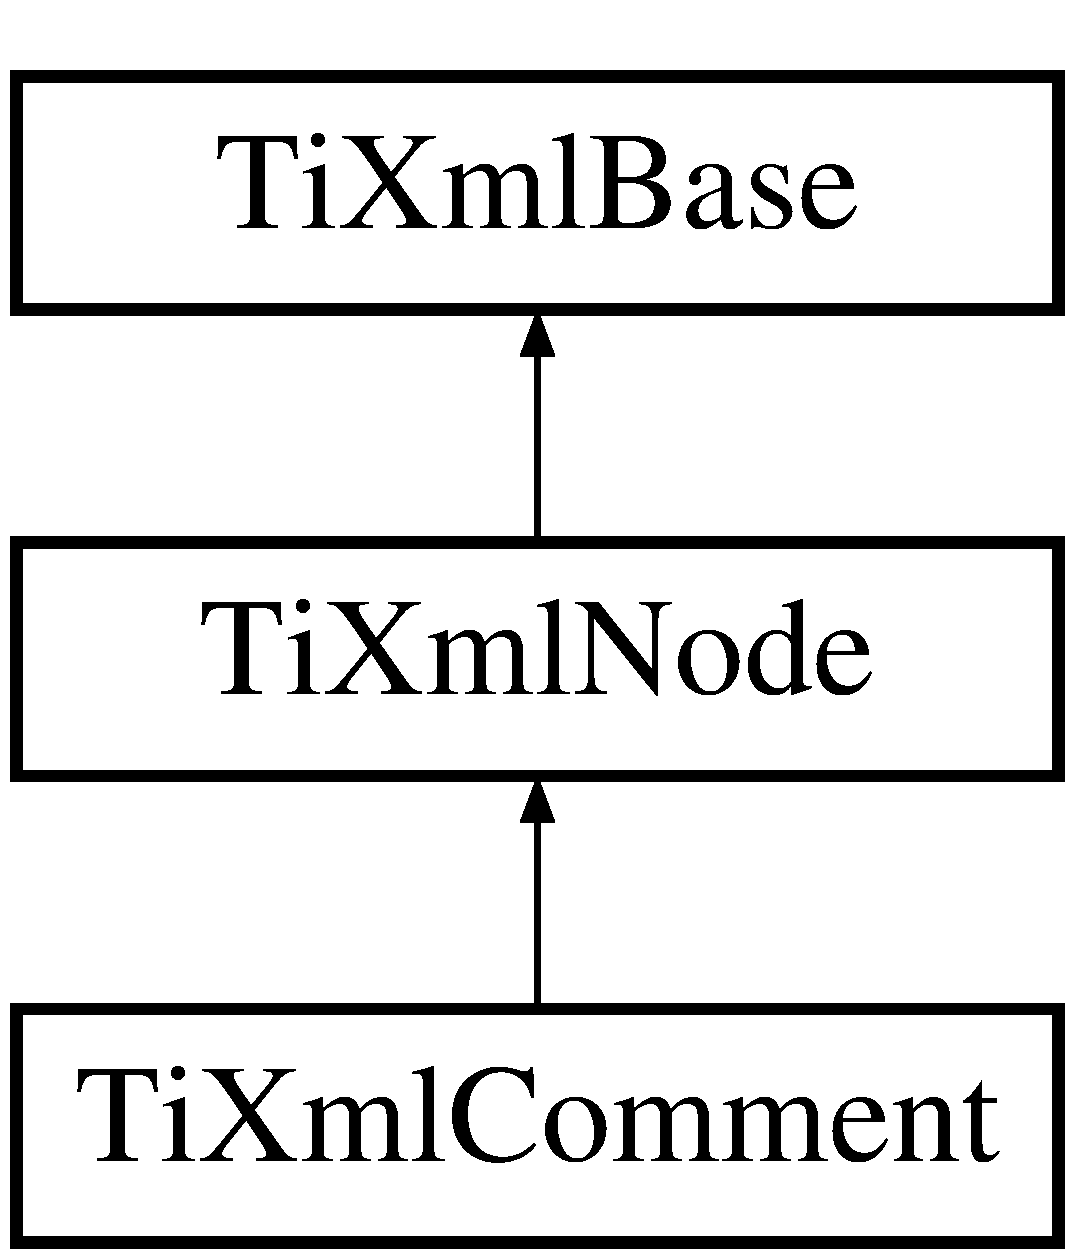
\includegraphics[height=3cm]{classTiXmlComment}
\end{center}
\end{figure}


\subsection{Detailed Description}
An XML comment. \subsection*{Public Member Functions}
\begin{CompactItemize}
\item 
{\bf TiXmlComment} ()
\begin{CompactList}\small\item\em Constructs an empty comment. \item\end{CompactList}\item 
{\bf TiXmlComment} (const char $\ast$\_\-value)
\begin{CompactList}\small\item\em Construct a comment from text. \item\end{CompactList}\item 
{\bf TiXmlComment} (const {\bf TiXmlComment} \&)
\item 
void {\bf operator=} (const {\bf TiXmlComment} \&base)
\item 
virtual {\bf $\sim$TiXmlComment} ()
\item 
virtual {\bf TiXmlNode} $\ast$ {\bf Clone} () const 
\begin{CompactList}\small\item\em Returns a copy of this Comment. \item\end{CompactList}\item 
virtual void {\bf Print} (FILE $\ast$cfile, int depth) const 
\item 
virtual const char $\ast$ {\bf Parse} (const char $\ast$p, {\bf TiXmlParsingData} $\ast$data, {\bf TiXmlEncoding} encoding)
\item 
virtual const {\bf TiXmlComment} $\ast$ {\bf ToComment} () const 
\begin{CompactList}\small\item\em Cast to a more defined type. Will return null not of the requested type. \item\end{CompactList}\item 
virtual {\bf TiXmlComment} $\ast$ {\bf ToComment} ()
\begin{CompactList}\small\item\em Cast to a more defined type. Will return null not of the requested type. \item\end{CompactList}\item 
virtual bool {\bf Accept} ({\bf TiXmlVisitor} $\ast$visitor) const 
\end{CompactItemize}
\subsection*{Protected Member Functions}
\begin{CompactItemize}
\item 
void {\bf CopyTo} ({\bf TiXmlComment} $\ast$target) const 
\end{CompactItemize}


\subsection{Constructor \& Destructor Documentation}
\index{TiXmlComment@{TiXmlComment}!TiXmlComment@{TiXmlComment}}
\index{TiXmlComment@{TiXmlComment}!TiXmlComment@{TiXmlComment}}
\subsubsection[TiXmlComment]{\setlength{\rightskip}{0pt plus 5cm}TiXmlComment::TiXmlComment ()\hspace{0.3cm}{\tt  [inline]}}\label{classTiXmlComment_aa3252031d3e8bd3a2bf51a1c61201b7}


Constructs an empty comment. 



Referenced by Clone().\index{TiXmlComment@{TiXmlComment}!TiXmlComment@{TiXmlComment}}
\index{TiXmlComment@{TiXmlComment}!TiXmlComment@{TiXmlComment}}
\subsubsection[TiXmlComment]{\setlength{\rightskip}{0pt plus 5cm}TiXmlComment::TiXmlComment (const char $\ast$ {\em \_\-value})\hspace{0.3cm}{\tt  [inline]}}\label{classTiXmlComment_37e7802ef17bc03ebe5ae79bf0713d47}


Construct a comment from text. 



References TiXmlNode::SetValue().\index{TiXmlComment@{TiXmlComment}!TiXmlComment@{TiXmlComment}}
\index{TiXmlComment@{TiXmlComment}!TiXmlComment@{TiXmlComment}}
\subsubsection[TiXmlComment]{\setlength{\rightskip}{0pt plus 5cm}TiXmlComment::TiXmlComment (const {\bf TiXmlComment} \& {\em copy})}\label{classTiXmlComment_faec41ac2760ce946ba1590eb5708e50}




References CopyTo().\index{TiXmlComment@{TiXmlComment}!$\sim$TiXmlComment@{$\sim$TiXmlComment}}
\index{$\sim$TiXmlComment@{$\sim$TiXmlComment}!TiXmlComment@{TiXmlComment}}
\subsubsection[$\sim$TiXmlComment]{\setlength{\rightskip}{0pt plus 5cm}virtual TiXmlComment::$\sim$TiXmlComment ()\hspace{0.3cm}{\tt  [inline, virtual]}}\label{classTiXmlComment_3264ae2e9c4a127edfa03289bb2c9aa2}




\subsection{Member Function Documentation}
\index{TiXmlComment@{TiXmlComment}!operator=@{operator=}}
\index{operator=@{operator=}!TiXmlComment@{TiXmlComment}}
\subsubsection[operator=]{\setlength{\rightskip}{0pt plus 5cm}void TiXmlComment::operator= (const {\bf TiXmlComment} \& {\em base})}\label{classTiXmlComment_46373f99b65cb960637dccb1f126bd49}




References TiXmlNode::Clear(), and CopyTo().\index{TiXmlComment@{TiXmlComment}!Clone@{Clone}}
\index{Clone@{Clone}!TiXmlComment@{TiXmlComment}}
\subsubsection[Clone]{\setlength{\rightskip}{0pt plus 5cm}{\bf TiXmlNode} $\ast$ TiXmlComment::Clone () const\hspace{0.3cm}{\tt  [virtual]}}\label{classTiXmlComment_4f6590c9c9a2b63a48972655b78eb853}


Returns a copy of this Comment. 



Implements {\bf TiXmlNode} \doxyref{}{p.}{classTiXmlNode_4508cc3a2d7a98e96a54cc09c37a78a4}.

References CopyTo(), and TiXmlComment().\index{TiXmlComment@{TiXmlComment}!Print@{Print}}
\index{Print@{Print}!TiXmlComment@{TiXmlComment}}
\subsubsection[Print]{\setlength{\rightskip}{0pt plus 5cm}void TiXmlComment::Print (FILE $\ast$ {\em cfile}, \/  int {\em depth}) const\hspace{0.3cm}{\tt  [virtual]}}\label{classTiXmlComment_17398061d62c470f57801ce28fa33ad4}


All TinyXml classes can print themselves to a filestream or the string class (\doxyref{TiXmlString}{p.}{classTiXmlString} in non-STL mode, std::string in STL mode.) Either or both cfile and str can be null.

This is a formatted print, and will insert tabs and newlines.

(For an unformatted stream, use the $<$$<$ operator.) 

Implements {\bf TiXmlBase} \doxyref{}{p.}{classTiXmlBase_0de56b3f2ef14c65091a3b916437b512}.

References TiXmlNode::value.\index{TiXmlComment@{TiXmlComment}!Parse@{Parse}}
\index{Parse@{Parse}!TiXmlComment@{TiXmlComment}}
\subsubsection[Parse]{\setlength{\rightskip}{0pt plus 5cm}const char $\ast$ TiXmlComment::Parse (const char $\ast$ {\em p}, \/  {\bf TiXmlParsingData} $\ast$ {\em data}, \/  {\bf TiXmlEncoding} {\em encoding})\hspace{0.3cm}{\tt  [virtual]}}\label{classTiXmlComment_43bddc18ac057734b41d84653b71d3e0}




Implements {\bf TiXmlBase} \doxyref{}{p.}{classTiXmlBase_00e4edb0219d00a1379c856e5a1d2025}.

References TiXmlParsingData::Cursor(), TiXmlNode::GetDocument(), TiXmlBase::location, TiXmlDocument::SetError(), TiXmlBase::SkipWhiteSpace(), TiXmlParsingData::Stamp(), TiXmlBase::StringEqual(), TiXmlBase::TIXML\_\-ERROR\_\-PARSING\_\-COMMENT, and TiXmlNode::value.\index{TiXmlComment@{TiXmlComment}!ToComment@{ToComment}}
\index{ToComment@{ToComment}!TiXmlComment@{TiXmlComment}}
\subsubsection[ToComment]{\setlength{\rightskip}{0pt plus 5cm}virtual const {\bf TiXmlComment}$\ast$ TiXmlComment::ToComment () const\hspace{0.3cm}{\tt  [inline, virtual]}}\label{classTiXmlComment_00fb4215c20a2399ea05ac9b9e7e68a0}


Cast to a more defined type. Will return null not of the requested type. 



Reimplemented from {\bf TiXmlNode} \doxyref{}{p.}{classTiXmlNode_a0a5086f9eaee910bbfdc7f975e26574}.\index{TiXmlComment@{TiXmlComment}!ToComment@{ToComment}}
\index{ToComment@{ToComment}!TiXmlComment@{TiXmlComment}}
\subsubsection[ToComment]{\setlength{\rightskip}{0pt plus 5cm}virtual {\bf TiXmlComment}$\ast$ TiXmlComment::ToComment ()\hspace{0.3cm}{\tt  [inline, virtual]}}\label{classTiXmlComment_cc7c7e07e13c23f17797d642981511df}


Cast to a more defined type. Will return null not of the requested type. 



Reimplemented from {\bf TiXmlNode} \doxyref{}{p.}{classTiXmlNode_383e06a0787f7063953934867990f849}.\index{TiXmlComment@{TiXmlComment}!Accept@{Accept}}
\index{Accept@{Accept}!TiXmlComment@{TiXmlComment}}
\subsubsection[Accept]{\setlength{\rightskip}{0pt plus 5cm}bool TiXmlComment::Accept ({\bf TiXmlVisitor} $\ast$ {\em visitor}) const\hspace{0.3cm}{\tt  [virtual]}}\label{classTiXmlComment_4382de0e50da973f11a23ea5852568bd}


Walk the XML tree visiting this node and all of its children. 

Implements {\bf TiXmlNode} \doxyref{}{p.}{classTiXmlNode_cc0f88b7462c6cb73809d410a4f5bb86}.

References TiXmlVisitor::Visit().\index{TiXmlComment@{TiXmlComment}!CopyTo@{CopyTo}}
\index{CopyTo@{CopyTo}!TiXmlComment@{TiXmlComment}}
\subsubsection[CopyTo]{\setlength{\rightskip}{0pt plus 5cm}void TiXmlComment::CopyTo ({\bf TiXmlComment} $\ast$ {\em target}) const\hspace{0.3cm}{\tt  [protected]}}\label{classTiXmlComment_3175b2f27628f4fb7a043897930cd934}




References TiXmlNode::CopyTo().

Referenced by Clone(), operator=(), and TiXmlComment().

The documentation for this class was generated from the following files:\begin{CompactItemize}
\item 
{\bf tinyxml.h}\item 
{\bf tinyxml.cpp}\item 
{\bf tinyxmlparser.cpp}\end{CompactItemize}

\section{TiXmlCursor Struct Reference}
\label{structTiXmlCursor}\index{TiXmlCursor@{TiXmlCursor}}
{\tt \#include $<$tinyxml.h$>$}

\subsection*{Public Member Functions}
\begin{CompactItemize}
\item 
{\bf TiXmlCursor} ()
\item 
void {\bf Clear} ()
\end{CompactItemize}
\subsection*{Public Attributes}
\begin{CompactItemize}
\item 
int {\bf row}
\item 
int {\bf col}
\end{CompactItemize}


\subsection{Constructor \& Destructor Documentation}
\index{TiXmlCursor@{TiXmlCursor}!TiXmlCursor@{TiXmlCursor}}
\index{TiXmlCursor@{TiXmlCursor}!TiXmlCursor@{TiXmlCursor}}
\subsubsection[TiXmlCursor]{\setlength{\rightskip}{0pt plus 5cm}TiXmlCursor::TiXmlCursor ()\hspace{0.3cm}{\tt  [inline]}}\label{structTiXmlCursor_7ad233928a675f0271eb440b150e3ff1}




References Clear().

\subsection{Member Function Documentation}
\index{TiXmlCursor@{TiXmlCursor}!Clear@{Clear}}
\index{Clear@{Clear}!TiXmlCursor@{TiXmlCursor}}
\subsubsection[Clear]{\setlength{\rightskip}{0pt plus 5cm}void TiXmlCursor::Clear ()\hspace{0.3cm}{\tt  [inline]}}\label{structTiXmlCursor_1e6fa622b59dafb71b6efe595105dcdd}




References col, and row.

Referenced by TiXmlDocument::LoadFile(), TiXmlDocument::Parse(), TiXmlDocument::SetError(), and TiXmlCursor().

\subsection{Member Data Documentation}
\index{TiXmlCursor@{TiXmlCursor}!row@{row}}
\index{row@{row}!TiXmlCursor@{TiXmlCursor}}
\subsubsection[row]{\setlength{\rightskip}{0pt plus 5cm}int {\bf TiXmlCursor::row}}\label{structTiXmlCursor_5b54dd949820c2db061e2be41f3effb3}




Referenced by Clear(), TiXmlDocument::ClearError(), TiXmlDocument::ErrorRow(), TiXmlDocument::Parse(), TiXmlBase::Row(), and TiXmlParsingData::Stamp().\index{TiXmlCursor@{TiXmlCursor}!col@{col}}
\index{col@{col}!TiXmlCursor@{TiXmlCursor}}
\subsubsection[col]{\setlength{\rightskip}{0pt plus 5cm}int {\bf TiXmlCursor::col}}\label{structTiXmlCursor_5694d7ed2c4d20109d350c14c417969d}




Referenced by Clear(), TiXmlDocument::ClearError(), TiXmlBase::Column(), TiXmlDocument::ErrorCol(), TiXmlDocument::Parse(), and TiXmlParsingData::Stamp().

The documentation for this struct was generated from the following file:\begin{CompactItemize}
\item 
{\bf tinyxml.h}\end{CompactItemize}

\section{TiXmlDeclaration Class Reference}
\label{classTiXmlDeclaration}\index{TiXmlDeclaration@{TiXmlDeclaration}}
{\tt \#include $<$tinyxml.h$>$}

Inheritance diagram for TiXmlDeclaration::\begin{figure}[H]
\begin{center}
\leavevmode
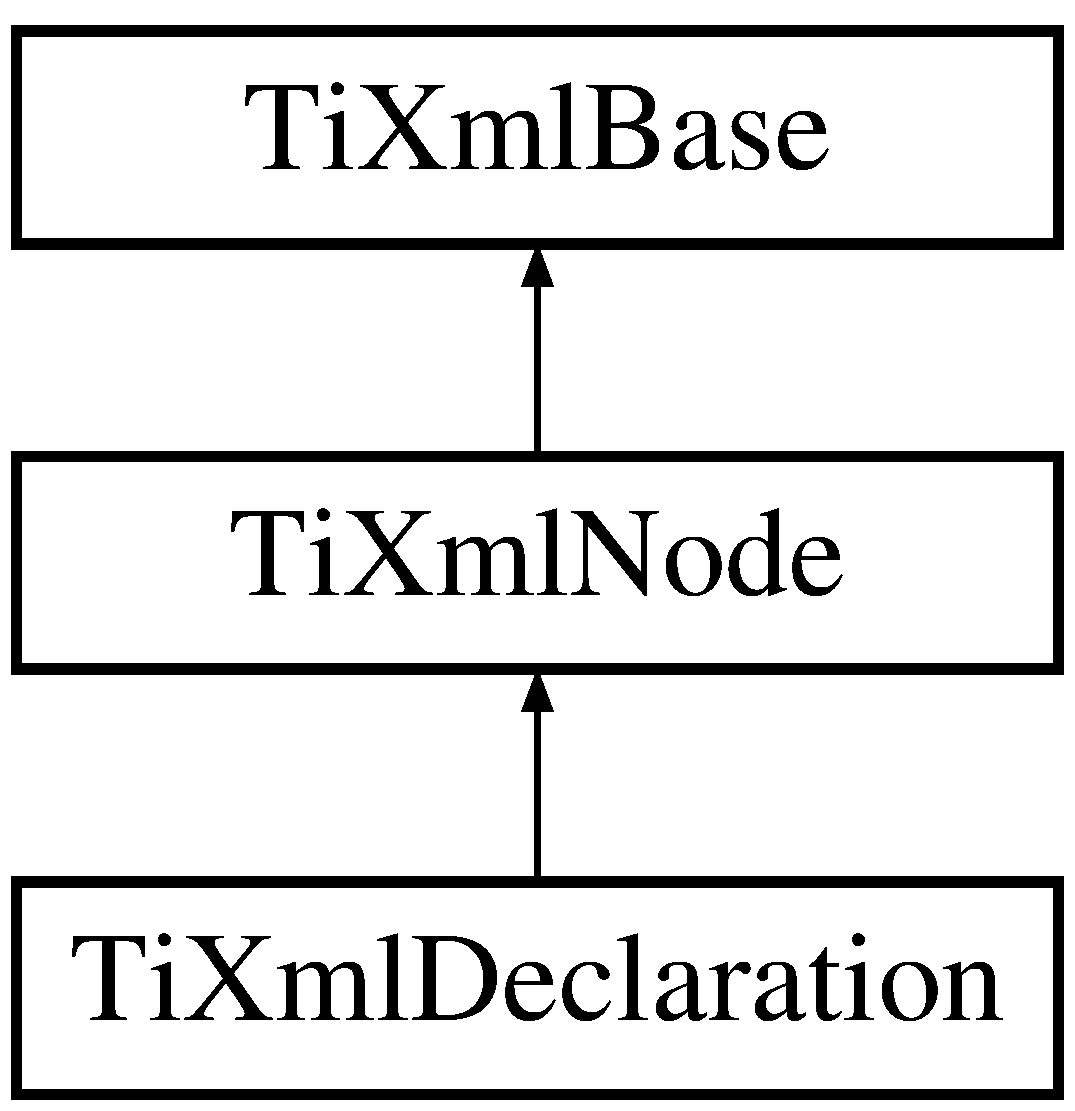
\includegraphics[height=3cm]{classTiXmlDeclaration}
\end{center}
\end{figure}


\subsection{Detailed Description}
In correct XML the declaration is the first entry in the file. 

\footnotesize\begin{verbatim}
		<?xml version="1.0" standalone="yes"?>
	\end{verbatim}
\normalsize


TinyXml will happily read or write files without a declaration, however. There are 3 possible attributes to the declaration: version, encoding, and standalone.

Note: In this version of the code, the attributes are handled as special cases, not generic attributes, simply because there can only be at most 3 and they are always the same. \subsection*{Public Member Functions}
\begin{CompactItemize}
\item 
{\bf TiXmlDeclaration} ()
\begin{CompactList}\small\item\em Construct an empty declaration. \item\end{CompactList}\item 
{\bf TiXmlDeclaration} (const char $\ast$\_\-version, const char $\ast$\_\-encoding, const char $\ast$\_\-standalone)
\begin{CompactList}\small\item\em Construct. \item\end{CompactList}\item 
{\bf TiXmlDeclaration} (const {\bf TiXmlDeclaration} \&copy)
\item 
void {\bf operator=} (const {\bf TiXmlDeclaration} \&copy)
\item 
virtual {\bf $\sim$TiXmlDeclaration} ()
\item 
const char $\ast$ {\bf Version} () const 
\begin{CompactList}\small\item\em Version. Will return an empty string if none was found. \item\end{CompactList}\item 
const char $\ast$ {\bf Encoding} () const 
\begin{CompactList}\small\item\em Encoding. Will return an empty string if none was found. \item\end{CompactList}\item 
const char $\ast$ {\bf Standalone} () const 
\begin{CompactList}\small\item\em Is this a standalone document? \item\end{CompactList}\item 
virtual {\bf TiXmlNode} $\ast$ {\bf Clone} () const 
\begin{CompactList}\small\item\em Creates a copy of this Declaration and returns it. \item\end{CompactList}\item 
virtual void {\bf Print} (FILE $\ast$cfile, int depth, TIXML\_\-STRING $\ast$str) const 
\item 
virtual void {\bf Print} (FILE $\ast$cfile, int depth) const 
\item 
virtual const char $\ast$ {\bf Parse} (const char $\ast$p, {\bf TiXmlParsingData} $\ast$data, {\bf TiXmlEncoding} encoding)
\item 
virtual const {\bf TiXmlDeclaration} $\ast$ {\bf ToDeclaration} () const 
\begin{CompactList}\small\item\em Cast to a more defined type. Will return null not of the requested type. \item\end{CompactList}\item 
virtual {\bf TiXmlDeclaration} $\ast$ {\bf ToDeclaration} ()
\begin{CompactList}\small\item\em Cast to a more defined type. Will return null not of the requested type. \item\end{CompactList}\item 
virtual bool {\bf Accept} ({\bf TiXmlVisitor} $\ast$visitor) const 
\end{CompactItemize}
\subsection*{Protected Member Functions}
\begin{CompactItemize}
\item 
void {\bf CopyTo} ({\bf TiXmlDeclaration} $\ast$target) const 
\end{CompactItemize}


\subsection{Constructor \& Destructor Documentation}
\index{TiXmlDeclaration@{TiXmlDeclaration}!TiXmlDeclaration@{TiXmlDeclaration}}
\index{TiXmlDeclaration@{TiXmlDeclaration}!TiXmlDeclaration@{TiXmlDeclaration}}
\subsubsection[TiXmlDeclaration]{\setlength{\rightskip}{0pt plus 5cm}TiXmlDeclaration::TiXmlDeclaration ()\hspace{0.3cm}{\tt  [inline]}}\label{classTiXmlDeclaration_a0484d059bea0ea1acb47c9094382d79}


Construct an empty declaration. 



Referenced by Clone().\index{TiXmlDeclaration@{TiXmlDeclaration}!TiXmlDeclaration@{TiXmlDeclaration}}
\index{TiXmlDeclaration@{TiXmlDeclaration}!TiXmlDeclaration@{TiXmlDeclaration}}
\subsubsection[TiXmlDeclaration]{\setlength{\rightskip}{0pt plus 5cm}TiXmlDeclaration::TiXmlDeclaration (const char $\ast$ {\em \_\-version}, \/  const char $\ast$ {\em \_\-encoding}, \/  const char $\ast$ {\em \_\-standalone})}\label{classTiXmlDeclaration_3b618d1c30c25e4b7a71f31a595ee298}


Construct. 

\index{TiXmlDeclaration@{TiXmlDeclaration}!TiXmlDeclaration@{TiXmlDeclaration}}
\index{TiXmlDeclaration@{TiXmlDeclaration}!TiXmlDeclaration@{TiXmlDeclaration}}
\subsubsection[TiXmlDeclaration]{\setlength{\rightskip}{0pt plus 5cm}TiXmlDeclaration::TiXmlDeclaration (const {\bf TiXmlDeclaration} \& {\em copy})}\label{classTiXmlDeclaration_58ac9042c342f7845c8491da0bb091e8}




References CopyTo().\index{TiXmlDeclaration@{TiXmlDeclaration}!$\sim$TiXmlDeclaration@{$\sim$TiXmlDeclaration}}
\index{$\sim$TiXmlDeclaration@{$\sim$TiXmlDeclaration}!TiXmlDeclaration@{TiXmlDeclaration}}
\subsubsection[$\sim$TiXmlDeclaration]{\setlength{\rightskip}{0pt plus 5cm}virtual TiXmlDeclaration::$\sim$TiXmlDeclaration ()\hspace{0.3cm}{\tt  [inline, virtual]}}\label{classTiXmlDeclaration_d5f37a673f4c507fd7e550470f9cec25}




\subsection{Member Function Documentation}
\index{TiXmlDeclaration@{TiXmlDeclaration}!operator=@{operator=}}
\index{operator=@{operator=}!TiXmlDeclaration@{TiXmlDeclaration}}
\subsubsection[operator=]{\setlength{\rightskip}{0pt plus 5cm}void TiXmlDeclaration::operator= (const {\bf TiXmlDeclaration} \& {\em copy})}\label{classTiXmlDeclaration_0fedc57539af9049be8db2d7d9d9ba33}




References TiXmlNode::Clear(), and CopyTo().\index{TiXmlDeclaration@{TiXmlDeclaration}!Version@{Version}}
\index{Version@{Version}!TiXmlDeclaration@{TiXmlDeclaration}}
\subsubsection[Version]{\setlength{\rightskip}{0pt plus 5cm}const char$\ast$ TiXmlDeclaration::Version () const\hspace{0.3cm}{\tt  [inline]}}\label{classTiXmlDeclaration_02ee557b1a4545c3219ed377c103ec76}


Version. Will return an empty string if none was found. 

\index{TiXmlDeclaration@{TiXmlDeclaration}!Encoding@{Encoding}}
\index{Encoding@{Encoding}!TiXmlDeclaration@{TiXmlDeclaration}}
\subsubsection[Encoding]{\setlength{\rightskip}{0pt plus 5cm}const char$\ast$ TiXmlDeclaration::Encoding () const\hspace{0.3cm}{\tt  [inline]}}\label{classTiXmlDeclaration_5d974231f9e9a2f0542f15f3a46cdb76}


Encoding. Will return an empty string if none was found. 



Referenced by TiXmlDocument::Parse().\index{TiXmlDeclaration@{TiXmlDeclaration}!Standalone@{Standalone}}
\index{Standalone@{Standalone}!TiXmlDeclaration@{TiXmlDeclaration}}
\subsubsection[Standalone]{\setlength{\rightskip}{0pt plus 5cm}const char$\ast$ TiXmlDeclaration::Standalone () const\hspace{0.3cm}{\tt  [inline]}}\label{classTiXmlDeclaration_9ff06afc033d7ef730ec7c6825b97ad9}


Is this a standalone document? 

\index{TiXmlDeclaration@{TiXmlDeclaration}!Clone@{Clone}}
\index{Clone@{Clone}!TiXmlDeclaration@{TiXmlDeclaration}}
\subsubsection[Clone]{\setlength{\rightskip}{0pt plus 5cm}{\bf TiXmlNode} $\ast$ TiXmlDeclaration::Clone () const\hspace{0.3cm}{\tt  [virtual]}}\label{classTiXmlDeclaration_ff8231266d735943d8a7514a9c9822b9}


Creates a copy of this Declaration and returns it. 



Implements {\bf TiXmlNode} \doxyref{}{p.}{classTiXmlNode_4508cc3a2d7a98e96a54cc09c37a78a4}.

References CopyTo(), and TiXmlDeclaration().\index{TiXmlDeclaration@{TiXmlDeclaration}!Print@{Print}}
\index{Print@{Print}!TiXmlDeclaration@{TiXmlDeclaration}}
\subsubsection[Print]{\setlength{\rightskip}{0pt plus 5cm}void TiXmlDeclaration::Print (FILE $\ast$ {\em cfile}, \/  int {\em depth}, \/  TIXML\_\-STRING $\ast$ {\em str}) const\hspace{0.3cm}{\tt  [virtual]}}\label{classTiXmlDeclaration_a5ab32ec19d4eeecff4a9238c6c90565}




Referenced by Print(), and TiXmlPrinter::Visit().\index{TiXmlDeclaration@{TiXmlDeclaration}!Print@{Print}}
\index{Print@{Print}!TiXmlDeclaration@{TiXmlDeclaration}}
\subsubsection[Print]{\setlength{\rightskip}{0pt plus 5cm}virtual void TiXmlDeclaration::Print (FILE $\ast$ {\em cfile}, \/  int {\em depth}) const\hspace{0.3cm}{\tt  [inline, virtual]}}\label{classTiXmlDeclaration_bf6303db4bd05b5be554036817ff1cb4}


All TinyXml classes can print themselves to a filestream or the string class (\doxyref{TiXmlString}{p.}{classTiXmlString} in non-STL mode, std::string in STL mode.) Either or both cfile and str can be null.

This is a formatted print, and will insert tabs and newlines.

(For an unformatted stream, use the $<$$<$ operator.) 

Implements {\bf TiXmlBase} \doxyref{}{p.}{classTiXmlBase_0de56b3f2ef14c65091a3b916437b512}.

References Print().\index{TiXmlDeclaration@{TiXmlDeclaration}!Parse@{Parse}}
\index{Parse@{Parse}!TiXmlDeclaration@{TiXmlDeclaration}}
\subsubsection[Parse]{\setlength{\rightskip}{0pt plus 5cm}const char $\ast$ TiXmlDeclaration::Parse (const char $\ast$ {\em p}, \/  {\bf TiXmlParsingData} $\ast$ {\em data}, \/  {\bf TiXmlEncoding} {\em encoding})\hspace{0.3cm}{\tt  [virtual]}}\label{classTiXmlDeclaration_9839ea97ed687a2b7342fd7b0f04361b}




Implements {\bf TiXmlBase} \doxyref{}{p.}{classTiXmlBase_00e4edb0219d00a1379c856e5a1d2025}.

References TiXmlParsingData::Cursor(), TiXmlNode::GetDocument(), TiXmlBase::IsWhiteSpace(), TiXmlBase::location, TiXmlAttribute::Parse(), TiXmlDocument::SetError(), TiXmlBase::SkipWhiteSpace(), TiXmlParsingData::Stamp(), TiXmlBase::StringEqual(), TiXmlBase::TIXML\_\-ERROR\_\-PARSING\_\-DECLARATION, and TiXmlAttribute::Value().\index{TiXmlDeclaration@{TiXmlDeclaration}!ToDeclaration@{ToDeclaration}}
\index{ToDeclaration@{ToDeclaration}!TiXmlDeclaration@{TiXmlDeclaration}}
\subsubsection[ToDeclaration]{\setlength{\rightskip}{0pt plus 5cm}virtual const {\bf TiXmlDeclaration}$\ast$ TiXmlDeclaration::ToDeclaration () const\hspace{0.3cm}{\tt  [inline, virtual]}}\label{classTiXmlDeclaration_1e085d3fefd1dbf5ccdbff729931a967}


Cast to a more defined type. Will return null not of the requested type. 



Reimplemented from {\bf TiXmlNode} \doxyref{}{p.}{classTiXmlNode_9f43e6984fc7d4afd6eb32714c6b7b72}.\index{TiXmlDeclaration@{TiXmlDeclaration}!ToDeclaration@{ToDeclaration}}
\index{ToDeclaration@{ToDeclaration}!TiXmlDeclaration@{TiXmlDeclaration}}
\subsubsection[ToDeclaration]{\setlength{\rightskip}{0pt plus 5cm}virtual {\bf TiXmlDeclaration}$\ast$ TiXmlDeclaration::ToDeclaration ()\hspace{0.3cm}{\tt  [inline, virtual]}}\label{classTiXmlDeclaration_6bd3d1daddcaeb9543c24bfd090969ce}


Cast to a more defined type. Will return null not of the requested type. 



Reimplemented from {\bf TiXmlNode} \doxyref{}{p.}{classTiXmlNode_4027136ca820ff4a636b607231b6a6df}.\index{TiXmlDeclaration@{TiXmlDeclaration}!Accept@{Accept}}
\index{Accept@{Accept}!TiXmlDeclaration@{TiXmlDeclaration}}
\subsubsection[Accept]{\setlength{\rightskip}{0pt plus 5cm}bool TiXmlDeclaration::Accept ({\bf TiXmlVisitor} $\ast$ {\em visitor}) const\hspace{0.3cm}{\tt  [virtual]}}\label{classTiXmlDeclaration_b6a6b178161ba9abc2c35058de689864}


Walk the XML tree visiting this node and all of its children. 

Implements {\bf TiXmlNode} \doxyref{}{p.}{classTiXmlNode_cc0f88b7462c6cb73809d410a4f5bb86}.

References TiXmlVisitor::Visit().\index{TiXmlDeclaration@{TiXmlDeclaration}!CopyTo@{CopyTo}}
\index{CopyTo@{CopyTo}!TiXmlDeclaration@{TiXmlDeclaration}}
\subsubsection[CopyTo]{\setlength{\rightskip}{0pt plus 5cm}void TiXmlDeclaration::CopyTo ({\bf TiXmlDeclaration} $\ast$ {\em target}) const\hspace{0.3cm}{\tt  [protected]}}\label{classTiXmlDeclaration_9d08959f935421a593032bd3efb30c38}




References TiXmlNode::CopyTo(), encoding, standalone, and version.

Referenced by Clone(), operator=(), and TiXmlDeclaration().

The documentation for this class was generated from the following files:\begin{CompactItemize}
\item 
{\bf tinyxml.h}\item 
{\bf tinyxml.cpp}\item 
{\bf tinyxmlparser.cpp}\end{CompactItemize}

\section{TiXmlDocument Class Reference}
\label{classTiXmlDocument}\index{TiXmlDocument@{TiXmlDocument}}
{\tt \#include $<$tinyxml.h$>$}

Inheritance diagram for TiXmlDocument::\begin{figure}[H]
\begin{center}
\leavevmode
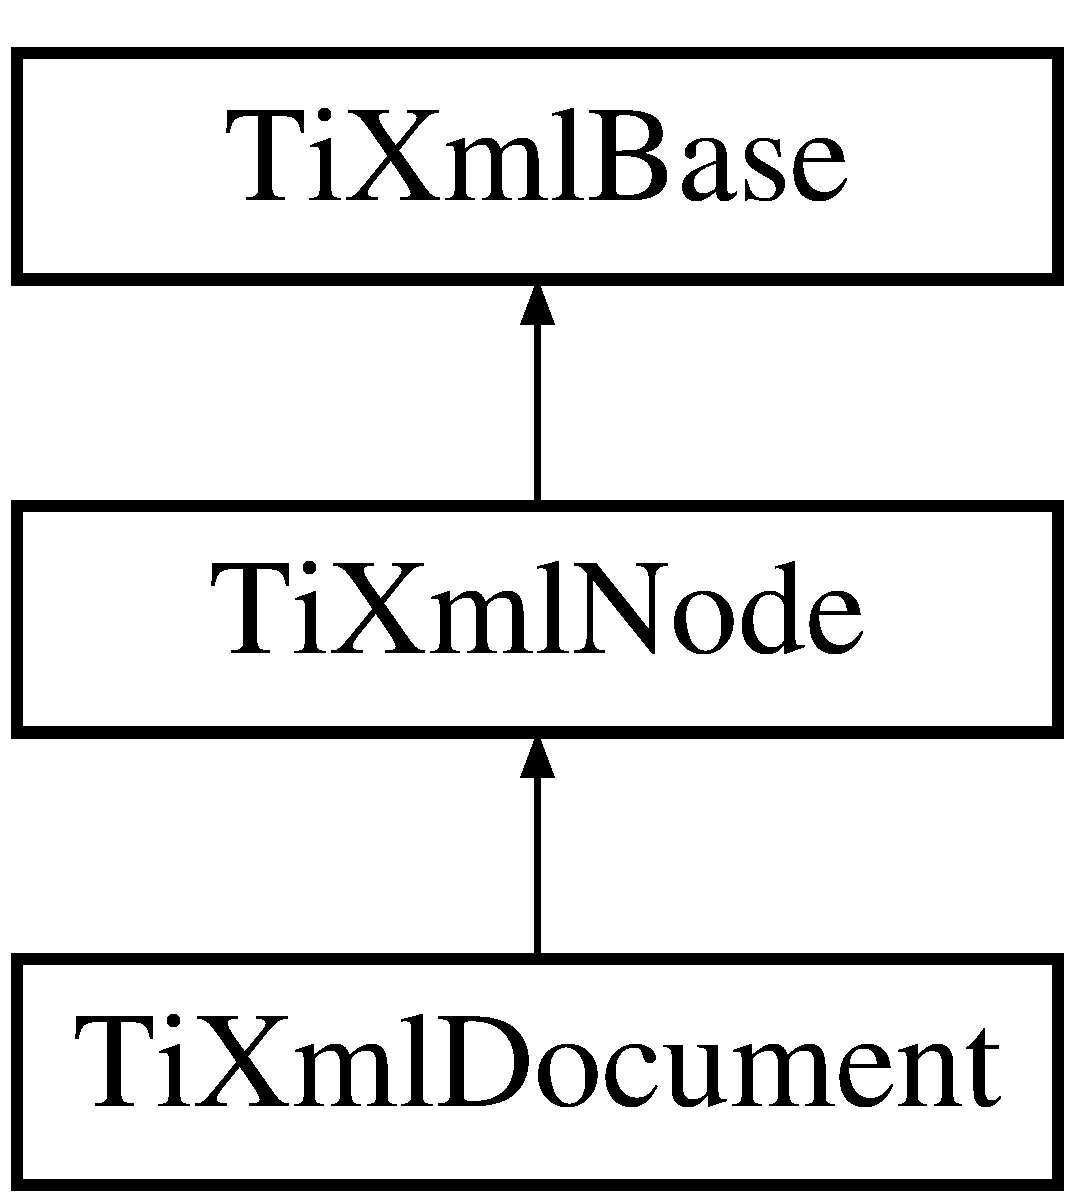
\includegraphics[height=3cm]{classTiXmlDocument}
\end{center}
\end{figure}


\subsection{Detailed Description}
Always the top level node. A document binds together all the XML pieces. It can be saved, loaded, and printed to the screen. The 'value' of a document node is the xml file name. \subsection*{Public Member Functions}
\begin{CompactItemize}
\item 
{\bf TiXmlDocument} ()
\begin{CompactList}\small\item\em Create an empty document, that has no name. \item\end{CompactList}\item 
{\bf TiXmlDocument} (const char $\ast$documentName)
\begin{CompactList}\small\item\em Create a document with a name. The name of the document is also the filename of the xml. \item\end{CompactList}\item 
{\bf TiXmlDocument} (const {\bf TiXmlDocument} \&copy)
\item 
void {\bf operator=} (const {\bf TiXmlDocument} \&copy)
\item 
virtual {\bf $\sim$TiXmlDocument} ()
\item 
bool {\bf LoadFile} ({\bf TiXmlEncoding} encoding={\bf TIXML\_\-DEFAULT\_\-ENCODING})
\item 
bool {\bf SaveFile} () const 
\begin{CompactList}\small\item\em Save a file using the current document value. Returns true if successful. \item\end{CompactList}\item 
bool {\bf LoadFile} (const char $\ast$filename, {\bf TiXmlEncoding} encoding={\bf TIXML\_\-DEFAULT\_\-ENCODING})
\begin{CompactList}\small\item\em Load a file using the given filename. Returns true if successful. \item\end{CompactList}\item 
bool {\bf SaveFile} (const char $\ast$filename) const 
\begin{CompactList}\small\item\em Save a file using the given filename. Returns true if successful. \item\end{CompactList}\item 
bool {\bf LoadFile} (FILE $\ast$, {\bf TiXmlEncoding} encoding={\bf TIXML\_\-DEFAULT\_\-ENCODING})
\item 
bool {\bf SaveFile} (FILE $\ast$) const 
\begin{CompactList}\small\item\em Save a file using the given FILE$\ast$. Returns true if successful. \item\end{CompactList}\item 
virtual const char $\ast$ {\bf Parse} (const char $\ast$p, {\bf TiXmlParsingData} $\ast$data=0, {\bf TiXmlEncoding} encoding={\bf TIXML\_\-DEFAULT\_\-ENCODING})
\item 
const {\bf TiXmlElement} $\ast$ {\bf RootElement} () const 
\item 
{\bf TiXmlElement} $\ast$ {\bf RootElement} ()
\item 
bool {\bf Error} () const 
\item 
const char $\ast$ {\bf ErrorDesc} () const 
\begin{CompactList}\small\item\em Contains a textual (english) description of the error if one occurs. \item\end{CompactList}\item 
int {\bf ErrorId} () const 
\item 
int {\bf ErrorRow} () const 
\item 
int {\bf ErrorCol} () const 
\begin{CompactList}\small\item\em The column where the error occured. See \doxyref{ErrorRow()}{p.}{classTiXmlDocument_f30efc75e804aa2e92fb8be3a8cb676e}. \item\end{CompactList}\item 
void {\bf SetTabSize} (int \_\-tabsize)
\item 
int {\bf TabSize} () const 
\item 
void {\bf ClearError} ()
\item 
void {\bf Print} () const 
\item 
virtual void {\bf Print} (FILE $\ast$cfile, int depth=0) const 
\begin{CompactList}\small\item\em Print this Document to a FILE stream. \item\end{CompactList}\item 
void {\bf SetError} (int err, const char $\ast$errorLocation, {\bf TiXmlParsingData} $\ast$prevData, {\bf TiXmlEncoding} encoding)
\item 
virtual const {\bf TiXmlDocument} $\ast$ {\bf ToDocument} () const 
\begin{CompactList}\small\item\em Cast to a more defined type. Will return null not of the requested type. \item\end{CompactList}\item 
virtual {\bf TiXmlDocument} $\ast$ {\bf ToDocument} ()
\begin{CompactList}\small\item\em Cast to a more defined type. Will return null not of the requested type. \item\end{CompactList}\item 
virtual bool {\bf Accept} ({\bf TiXmlVisitor} $\ast$content) const 
\end{CompactItemize}
\subsection*{Protected Member Functions}
\begin{CompactItemize}
\item 
virtual {\bf TiXmlNode} $\ast$ {\bf Clone} () const 
\end{CompactItemize}


\subsection{Constructor \& Destructor Documentation}
\index{TiXmlDocument@{TiXmlDocument}!TiXmlDocument@{TiXmlDocument}}
\index{TiXmlDocument@{TiXmlDocument}!TiXmlDocument@{TiXmlDocument}}
\subsubsection[TiXmlDocument]{\setlength{\rightskip}{0pt plus 5cm}TiXmlDocument::TiXmlDocument ()}\label{classTiXmlDocument_9f5e84335708fde98400230f9f12659c}


Create an empty document, that has no name. 



References ClearError().

Referenced by Clone().\index{TiXmlDocument@{TiXmlDocument}!TiXmlDocument@{TiXmlDocument}}
\index{TiXmlDocument@{TiXmlDocument}!TiXmlDocument@{TiXmlDocument}}
\subsubsection[TiXmlDocument]{\setlength{\rightskip}{0pt plus 5cm}TiXmlDocument::TiXmlDocument (const char $\ast$ {\em documentName})}\label{classTiXmlDocument_e4508b452d0c3061db085f3db27b8396}


Create a document with a name. The name of the document is also the filename of the xml. 



References ClearError(), and TiXmlNode::value.\index{TiXmlDocument@{TiXmlDocument}!TiXmlDocument@{TiXmlDocument}}
\index{TiXmlDocument@{TiXmlDocument}!TiXmlDocument@{TiXmlDocument}}
\subsubsection[TiXmlDocument]{\setlength{\rightskip}{0pt plus 5cm}TiXmlDocument::TiXmlDocument (const {\bf TiXmlDocument} \& {\em copy})}\label{classTiXmlDocument_323a7486e7da6099cdc19a5ff7e74b07}




References CopyTo().\index{TiXmlDocument@{TiXmlDocument}!$\sim$TiXmlDocument@{$\sim$TiXmlDocument}}
\index{$\sim$TiXmlDocument@{$\sim$TiXmlDocument}!TiXmlDocument@{TiXmlDocument}}
\subsubsection[$\sim$TiXmlDocument]{\setlength{\rightskip}{0pt plus 5cm}virtual TiXmlDocument::$\sim$TiXmlDocument ()\hspace{0.3cm}{\tt  [inline, virtual]}}\label{classTiXmlDocument_1b8a035c2c2aab38e4387246a0b712c5}




\subsection{Member Function Documentation}
\index{TiXmlDocument@{TiXmlDocument}!operator=@{operator=}}
\index{operator=@{operator=}!TiXmlDocument@{TiXmlDocument}}
\subsubsection[operator=]{\setlength{\rightskip}{0pt plus 5cm}void TiXmlDocument::operator= (const {\bf TiXmlDocument} \& {\em copy})}\label{classTiXmlDocument_afbfacc3414008f619b1345775ef12a4}




References TiXmlNode::Clear(), and CopyTo().\index{TiXmlDocument@{TiXmlDocument}!LoadFile@{LoadFile}}
\index{LoadFile@{LoadFile}!TiXmlDocument@{TiXmlDocument}}
\subsubsection[LoadFile]{\setlength{\rightskip}{0pt plus 5cm}bool TiXmlDocument::LoadFile ({\bf TiXmlEncoding} {\em encoding} = {\tt {\bf TIXML\_\-DEFAULT\_\-ENCODING}})}\label{classTiXmlDocument_4c852a889c02cf251117fd1d9fe1845f}


Load a file using the current document value. Returns true if successful. Will delete any existing document data before loading. 

References TiXmlNode::Value().

Referenced by LoadFile().\index{TiXmlDocument@{TiXmlDocument}!SaveFile@{SaveFile}}
\index{SaveFile@{SaveFile}!TiXmlDocument@{TiXmlDocument}}
\subsubsection[SaveFile]{\setlength{\rightskip}{0pt plus 5cm}bool TiXmlDocument::SaveFile () const}\label{classTiXmlDocument_21c0aeb0d0a720169ad4ac89523ebe93}


Save a file using the current document value. Returns true if successful. 



References TiXmlNode::Value().

Referenced by SaveFile().\index{TiXmlDocument@{TiXmlDocument}!LoadFile@{LoadFile}}
\index{LoadFile@{LoadFile}!TiXmlDocument@{TiXmlDocument}}
\subsubsection[LoadFile]{\setlength{\rightskip}{0pt plus 5cm}bool TiXmlDocument::LoadFile (const char $\ast$ {\em filename}, \/  {\bf TiXmlEncoding} {\em encoding} = {\tt {\bf TIXML\_\-DEFAULT\_\-ENCODING}})}\label{classTiXmlDocument_879cdf5e981b8b2d2ef82f2546dd28fb}


Load a file using the given filename. Returns true if successful. 



References LoadFile(), SetError(), TIXML\_\-ENCODING\_\-UNKNOWN, TiXmlBase::TIXML\_\-ERROR\_\-OPENING\_\-FILE, TIXML\_\-STRING, TiXmlFOpen(), and TiXmlNode::value.\index{TiXmlDocument@{TiXmlDocument}!SaveFile@{SaveFile}}
\index{SaveFile@{SaveFile}!TiXmlDocument@{TiXmlDocument}}
\subsubsection[SaveFile]{\setlength{\rightskip}{0pt plus 5cm}bool TiXmlDocument::SaveFile (const char $\ast$ {\em filename}) const}\label{classTiXmlDocument_e869f5ebf7fc54c4a1d737fb4689fd44}


Save a file using the given filename. Returns true if successful. 



References SaveFile(), and TiXmlFOpen().\index{TiXmlDocument@{TiXmlDocument}!LoadFile@{LoadFile}}
\index{LoadFile@{LoadFile}!TiXmlDocument@{TiXmlDocument}}
\subsubsection[LoadFile]{\setlength{\rightskip}{0pt plus 5cm}bool TiXmlDocument::LoadFile (FILE $\ast$ {\em file}, \/  {\bf TiXmlEncoding} {\em encoding} = {\tt {\bf TIXML\_\-DEFAULT\_\-ENCODING}})}\label{classTiXmlDocument_41f6fe7200864d1dca663d230caf8db6}


Load a file using the given FILE$\ast$. Returns true if successful. Note that this method doesn't stream - the entire object pointed at by the FILE$\ast$ will be interpreted as an XML file. TinyXML doesn't stream in XML from the current file location. Streaming may be added in the future. 

References TiXmlCursor::Clear(), TiXmlNode::Clear(), Error(), TiXmlBase::location, Parse(), SetError(), TIXML\_\-ENCODING\_\-UNKNOWN, TiXmlBase::TIXML\_\-ERROR\_\-DOCUMENT\_\-EMPTY, TiXmlBase::TIXML\_\-ERROR\_\-OPENING\_\-FILE, and TIXML\_\-STRING.\index{TiXmlDocument@{TiXmlDocument}!SaveFile@{SaveFile}}
\index{SaveFile@{SaveFile}!TiXmlDocument@{TiXmlDocument}}
\subsubsection[SaveFile]{\setlength{\rightskip}{0pt plus 5cm}bool TiXmlDocument::SaveFile (FILE $\ast$ {\em fp}) const}\label{classTiXmlDocument_cf1672b4538c6d1d441f9f108aea2bf4}


Save a file using the given FILE$\ast$. Returns true if successful. 



References Print(), TIXML\_\-UTF\_\-LEAD\_\-0, TIXML\_\-UTF\_\-LEAD\_\-1, and TIXML\_\-UTF\_\-LEAD\_\-2.\index{TiXmlDocument@{TiXmlDocument}!Parse@{Parse}}
\index{Parse@{Parse}!TiXmlDocument@{TiXmlDocument}}
\subsubsection[Parse]{\setlength{\rightskip}{0pt plus 5cm}const char $\ast$ TiXmlDocument::Parse (const char $\ast$ {\em p}, \/  {\bf TiXmlParsingData} $\ast$ {\em data} = {\tt 0}, \/  {\bf TiXmlEncoding} {\em encoding} = {\tt {\bf TIXML\_\-DEFAULT\_\-ENCODING}})\hspace{0.3cm}{\tt  [virtual]}}\label{classTiXmlDocument_789ad2f06f93d52bdb5570b2f3670289}


Parse the given null terminated block of xml data. Passing in an encoding to this method (either TIXML\_\-ENCODING\_\-LEGACY or TIXML\_\-ENCODING\_\-UTF8 will force TinyXml to use that encoding, regardless of what TinyXml might otherwise try to detect. 

Implements {\bf TiXmlBase} \doxyref{}{p.}{classTiXmlBase_00e4edb0219d00a1379c856e5a1d2025}.

References TiXmlCursor::Clear(), ClearError(), TiXmlCursor::col, TiXmlParsingData::Cursor(), TiXmlParsingData::cursor, TiXmlDeclaration::Encoding(), TiXmlNode::firstChild, TiXmlNode::Identify(), TiXmlNode::LinkEndChild(), TiXmlBase::location, TiXmlBase::Parse(), TiXmlCursor::row, SetError(), TiXmlBase::SkipWhiteSpace(), TiXmlBase::StringEqual(), TabSize(), TIXML\_\-ENCODING\_\-LEGACY, TIXML\_\-ENCODING\_\-UNKNOWN, TIXML\_\-ENCODING\_\-UTF8, TiXmlBase::TIXML\_\-ERROR\_\-DOCUMENT\_\-EMPTY, TIXML\_\-UTF\_\-LEAD\_\-0, TIXML\_\-UTF\_\-LEAD\_\-1, TIXML\_\-UTF\_\-LEAD\_\-2, and TiXmlNode::ToDeclaration().

Referenced by LoadFile().\index{TiXmlDocument@{TiXmlDocument}!RootElement@{RootElement}}
\index{RootElement@{RootElement}!TiXmlDocument@{TiXmlDocument}}
\subsubsection[RootElement]{\setlength{\rightskip}{0pt plus 5cm}const {\bf TiXmlElement}$\ast$ TiXmlDocument::RootElement () const\hspace{0.3cm}{\tt  [inline]}}\label{classTiXmlDocument_d09d17927f908f40efb406af2fb873be}


Get the root element -- the only top level element -- of the document. In well formed XML, there should only be one. TinyXml is tolerant of multiple elements at the document level. 

References TiXmlNode::FirstChildElement().\index{TiXmlDocument@{TiXmlDocument}!RootElement@{RootElement}}
\index{RootElement@{RootElement}!TiXmlDocument@{TiXmlDocument}}
\subsubsection[RootElement]{\setlength{\rightskip}{0pt plus 5cm}{\bf TiXmlElement}$\ast$ TiXmlDocument::RootElement ()\hspace{0.3cm}{\tt  [inline]}}\label{classTiXmlDocument_0b43e762a23f938b06651bc90b8a1013}




References TiXmlNode::FirstChildElement().\index{TiXmlDocument@{TiXmlDocument}!Error@{Error}}
\index{Error@{Error}!TiXmlDocument@{TiXmlDocument}}
\subsubsection[Error]{\setlength{\rightskip}{0pt plus 5cm}bool TiXmlDocument::Error () const\hspace{0.3cm}{\tt  [inline]}}\label{classTiXmlDocument_6dfc01a6e5d58e56acd537dfd3bdeb29}


If an error occurs, Error will be set to true. Also,\begin{itemize}
\item The \doxyref{ErrorId()}{p.}{classTiXmlDocument_f96fc2f3f9ec6422782bfe916c9e778f} will contain the integer identifier of the error (not generally useful)\item The \doxyref{ErrorDesc()}{p.}{classTiXmlDocument_9d0f689f6e09ea494ea547be8d79c25e} method will return the name of the error. (very useful)\item The \doxyref{ErrorRow()}{p.}{classTiXmlDocument_f30efc75e804aa2e92fb8be3a8cb676e} and \doxyref{ErrorCol()}{p.}{classTiXmlDocument_a90bc630ee5203c6109ca5fad3323649} will return the location of the error (if known) \end{itemize}


Referenced by LoadFile().\index{TiXmlDocument@{TiXmlDocument}!ErrorDesc@{ErrorDesc}}
\index{ErrorDesc@{ErrorDesc}!TiXmlDocument@{TiXmlDocument}}
\subsubsection[ErrorDesc]{\setlength{\rightskip}{0pt plus 5cm}const char$\ast$ TiXmlDocument::ErrorDesc () const\hspace{0.3cm}{\tt  [inline]}}\label{classTiXmlDocument_9d0f689f6e09ea494ea547be8d79c25e}


Contains a textual (english) description of the error if one occurs. 

\index{TiXmlDocument@{TiXmlDocument}!ErrorId@{ErrorId}}
\index{ErrorId@{ErrorId}!TiXmlDocument@{TiXmlDocument}}
\subsubsection[ErrorId]{\setlength{\rightskip}{0pt plus 5cm}int TiXmlDocument::ErrorId () const\hspace{0.3cm}{\tt  [inline]}}\label{classTiXmlDocument_f96fc2f3f9ec6422782bfe916c9e778f}


Generally, you probably want the error string ( \doxyref{ErrorDesc()}{p.}{classTiXmlDocument_9d0f689f6e09ea494ea547be8d79c25e} ). But if you prefer the ErrorId, this function will fetch it. \index{TiXmlDocument@{TiXmlDocument}!ErrorRow@{ErrorRow}}
\index{ErrorRow@{ErrorRow}!TiXmlDocument@{TiXmlDocument}}
\subsubsection[ErrorRow]{\setlength{\rightskip}{0pt plus 5cm}int TiXmlDocument::ErrorRow () const\hspace{0.3cm}{\tt  [inline]}}\label{classTiXmlDocument_f30efc75e804aa2e92fb8be3a8cb676e}


Returns the location (if known) of the error. The first column is column 1, and the first row is row 1. A value of 0 means the row and column wasn't applicable (memory errors, for example, have no row/column) or the parser lost the error. (An error in the error reporting, in that case.)

\begin{Desc}
\item[See also:]\doxyref{SetTabSize}{p.}{classTiXmlDocument_51dac56316f89b35bdb7d0d433ba988e}, \doxyref{Row}{p.}{classTiXmlBase_024bceb070188df92c2a8d8852dd0853}, \doxyref{Column}{p.}{classTiXmlBase_b54bfb9b70fe6dd276e7b279cab7f003} \end{Desc}


References TiXmlCursor::row.\index{TiXmlDocument@{TiXmlDocument}!ErrorCol@{ErrorCol}}
\index{ErrorCol@{ErrorCol}!TiXmlDocument@{TiXmlDocument}}
\subsubsection[ErrorCol]{\setlength{\rightskip}{0pt plus 5cm}int TiXmlDocument::ErrorCol () const\hspace{0.3cm}{\tt  [inline]}}\label{classTiXmlDocument_a90bc630ee5203c6109ca5fad3323649}


The column where the error occured. See \doxyref{ErrorRow()}{p.}{classTiXmlDocument_f30efc75e804aa2e92fb8be3a8cb676e}. 



References TiXmlCursor::col.\index{TiXmlDocument@{TiXmlDocument}!SetTabSize@{SetTabSize}}
\index{SetTabSize@{SetTabSize}!TiXmlDocument@{TiXmlDocument}}
\subsubsection[SetTabSize]{\setlength{\rightskip}{0pt plus 5cm}void TiXmlDocument::SetTabSize (int {\em \_\-tabsize})\hspace{0.3cm}{\tt  [inline]}}\label{classTiXmlDocument_51dac56316f89b35bdb7d0d433ba988e}


\doxyref{SetTabSize()}{p.}{classTiXmlDocument_51dac56316f89b35bdb7d0d433ba988e} allows the error reporting functions (\doxyref{ErrorRow()}{p.}{classTiXmlDocument_f30efc75e804aa2e92fb8be3a8cb676e} and \doxyref{ErrorCol()}{p.}{classTiXmlDocument_a90bc630ee5203c6109ca5fad3323649}) to report the correct values for row and column. It does not change the output or input in any way.

By calling this method, with a tab size greater than 0, the row and column of each node and attribute is stored when the file is loaded. Very useful for tracking the DOM back in to the source file.

The tab size is required for calculating the location of nodes. If not set, the default of 4 is used. The tabsize is set per document. Setting the tabsize to 0 disables row/column tracking.

Note that row and column tracking is not supported when using operator$>$$>$.

The tab size needs to be enabled before the parse or load. Correct usage: 

\footnotesize\begin{verbatim}
		TiXmlDocument doc;
		doc.SetTabSize( 8 );
		doc.Load( "myfile.xml" );
		\end{verbatim}
\normalsize


\begin{Desc}
\item[See also:]\doxyref{Row}{p.}{classTiXmlBase_024bceb070188df92c2a8d8852dd0853}, \doxyref{Column}{p.}{classTiXmlBase_b54bfb9b70fe6dd276e7b279cab7f003} \end{Desc}
\index{TiXmlDocument@{TiXmlDocument}!TabSize@{TabSize}}
\index{TabSize@{TabSize}!TiXmlDocument@{TiXmlDocument}}
\subsubsection[TabSize]{\setlength{\rightskip}{0pt plus 5cm}int TiXmlDocument::TabSize () const\hspace{0.3cm}{\tt  [inline]}}\label{classTiXmlDocument_612360241b85bad0826b2a9ae9cda561}




Referenced by Parse().\index{TiXmlDocument@{TiXmlDocument}!ClearError@{ClearError}}
\index{ClearError@{ClearError}!TiXmlDocument@{TiXmlDocument}}
\subsubsection[ClearError]{\setlength{\rightskip}{0pt plus 5cm}void TiXmlDocument::ClearError ()\hspace{0.3cm}{\tt  [inline]}}\label{classTiXmlDocument_c66b8c28db86363315712a3574e87c35}


If you have handled the error, it can be reset with this call. The error state is automatically cleared if you Parse a new XML block. 

References TiXmlCursor::col, and TiXmlCursor::row.

Referenced by Parse(), and TiXmlDocument().\index{TiXmlDocument@{TiXmlDocument}!Print@{Print}}
\index{Print@{Print}!TiXmlDocument@{TiXmlDocument}}
\subsubsection[Print]{\setlength{\rightskip}{0pt plus 5cm}void TiXmlDocument::Print () const\hspace{0.3cm}{\tt  [inline]}}\label{classTiXmlDocument_f08389ec70ee9b2de7f800e206a18510}


Write the document to standard out using formatted printing (\char`\"{}pretty print\char`\"{}). 

Referenced by SaveFile().\index{TiXmlDocument@{TiXmlDocument}!Print@{Print}}
\index{Print@{Print}!TiXmlDocument@{TiXmlDocument}}
\subsubsection[Print]{\setlength{\rightskip}{0pt plus 5cm}void TiXmlDocument::Print (FILE $\ast$ {\em cfile}, \/  int {\em depth} = {\tt 0}) const\hspace{0.3cm}{\tt  [virtual]}}\label{classTiXmlDocument_7b1aea204fee266b70b9c105c8bf2ada}


Print this Document to a FILE stream. 



Implements {\bf TiXmlBase} \doxyref{}{p.}{classTiXmlBase_0de56b3f2ef14c65091a3b916437b512}.

References TiXmlNode::FirstChild(), TiXmlNode::NextSibling(), and TiXmlBase::Print().\index{TiXmlDocument@{TiXmlDocument}!SetError@{SetError}}
\index{SetError@{SetError}!TiXmlDocument@{TiXmlDocument}}
\subsubsection[SetError]{\setlength{\rightskip}{0pt plus 5cm}void TiXmlDocument::SetError (int {\em err}, \/  const char $\ast$ {\em errorLocation}, \/  {\bf TiXmlParsingData} $\ast$ {\em prevData}, \/  {\bf TiXmlEncoding} {\em encoding})}\label{classTiXmlDocument_735c23e318597b920c94eae77fa206de}




References TiXmlCursor::Clear(), TiXmlParsingData::Cursor(), TiXmlBase::errorString, TiXmlParsingData::Stamp(), and TiXmlBase::TIXML\_\-ERROR\_\-STRING\_\-COUNT.

Referenced by TiXmlNode::Identify(), TiXmlNode::InsertAfterChild(), TiXmlNode::InsertBeforeChild(), TiXmlNode::InsertEndChild(), TiXmlNode::LinkEndChild(), LoadFile(), TiXmlDeclaration::Parse(), TiXmlText::Parse(), TiXmlAttribute::Parse(), TiXmlComment::Parse(), TiXmlUnknown::Parse(), TiXmlElement::Parse(), Parse(), TiXmlElement::ReadValue(), and TiXmlElement::SetAttribute().\index{TiXmlDocument@{TiXmlDocument}!ToDocument@{ToDocument}}
\index{ToDocument@{ToDocument}!TiXmlDocument@{TiXmlDocument}}
\subsubsection[ToDocument]{\setlength{\rightskip}{0pt plus 5cm}virtual const {\bf TiXmlDocument}$\ast$ TiXmlDocument::ToDocument () const\hspace{0.3cm}{\tt  [inline, virtual]}}\label{classTiXmlDocument_1dc977bde3e4fe85a8eb9d88a35ef5a4}


Cast to a more defined type. Will return null not of the requested type. 



Reimplemented from {\bf TiXmlNode} \doxyref{}{p.}{classTiXmlNode_8a4cda4b15c29f64cff419309aebed08}.\index{TiXmlDocument@{TiXmlDocument}!ToDocument@{ToDocument}}
\index{ToDocument@{ToDocument}!TiXmlDocument@{TiXmlDocument}}
\subsubsection[ToDocument]{\setlength{\rightskip}{0pt plus 5cm}virtual {\bf TiXmlDocument}$\ast$ TiXmlDocument::ToDocument ()\hspace{0.3cm}{\tt  [inline, virtual]}}\label{classTiXmlDocument_1025d942a1f328fd742d545e37efdd42}


Cast to a more defined type. Will return null not of the requested type. 



Reimplemented from {\bf TiXmlNode} \doxyref{}{p.}{classTiXmlNode_6a4c8ac28ee7a745d059db6691e03bae}.\index{TiXmlDocument@{TiXmlDocument}!Accept@{Accept}}
\index{Accept@{Accept}!TiXmlDocument@{TiXmlDocument}}
\subsubsection[Accept]{\setlength{\rightskip}{0pt plus 5cm}bool TiXmlDocument::Accept ({\bf TiXmlVisitor} $\ast$ {\em content}) const\hspace{0.3cm}{\tt  [virtual]}}\label{classTiXmlDocument_3daab2f472418ef66315750202f762ae}


Walk the XML tree visiting this node and all of its children. 

Implements {\bf TiXmlNode} \doxyref{}{p.}{classTiXmlNode_cc0f88b7462c6cb73809d410a4f5bb86}.

References TiXmlNode::Accept(), TiXmlNode::FirstChild(), TiXmlNode::NextSibling(), TiXmlVisitor::VisitEnter(), and TiXmlVisitor::VisitExit().\index{TiXmlDocument@{TiXmlDocument}!Clone@{Clone}}
\index{Clone@{Clone}!TiXmlDocument@{TiXmlDocument}}
\subsubsection[Clone]{\setlength{\rightskip}{0pt plus 5cm}{\bf TiXmlNode} $\ast$ TiXmlDocument::Clone () const\hspace{0.3cm}{\tt  [protected, virtual]}}\label{classTiXmlDocument_c9e8f09b23454d953b32d1b65cd1409e}


Create an exact duplicate of this node and return it. The memory must be deleted by the caller. 

Implements {\bf TiXmlNode} \doxyref{}{p.}{classTiXmlNode_4508cc3a2d7a98e96a54cc09c37a78a4}.

References TiXmlDocument().

The documentation for this class was generated from the following files:\begin{CompactItemize}
\item 
{\bf tinyxml.h}\item 
{\bf tinyxml.cpp}\item 
{\bf tinyxmlparser.cpp}\end{CompactItemize}

\section{TiXmlElement Class Reference}
\label{classTiXmlElement}\index{TiXmlElement@{TiXmlElement}}
{\tt \#include $<$tinyxml.h$>$}

Inheritance diagram for TiXmlElement::\begin{figure}[H]
\begin{center}
\leavevmode
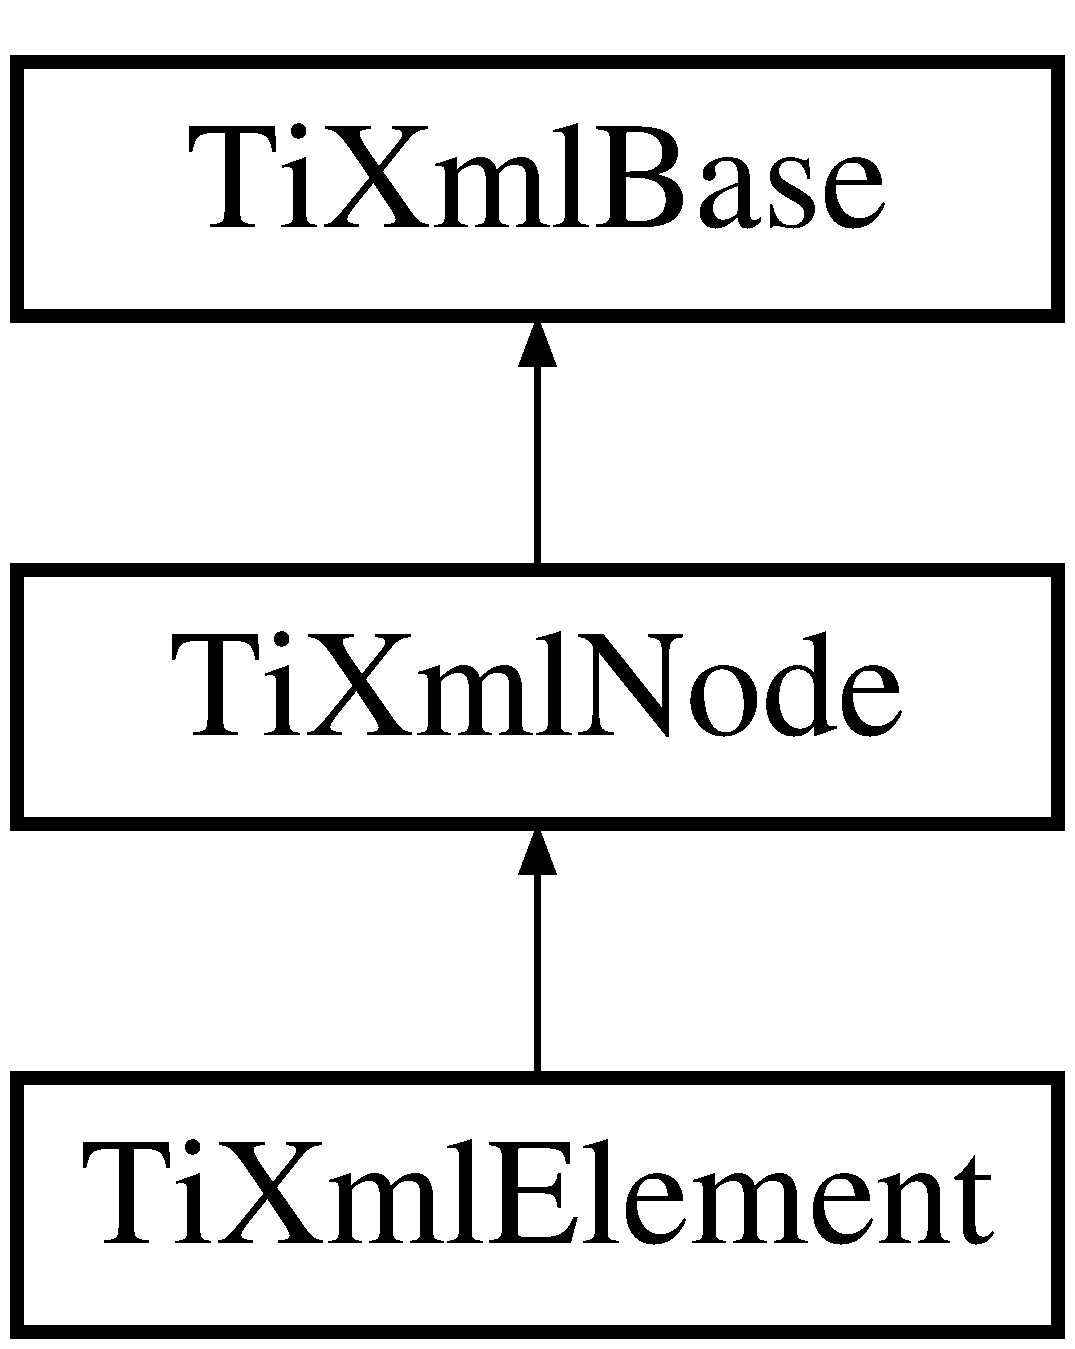
\includegraphics[height=3cm]{classTiXmlElement}
\end{center}
\end{figure}


\subsection{Detailed Description}
The element is a container class. It has a value, the element name, and can contain other elements, text, comments, and unknowns. Elements also contain an arbitrary number of attributes. \subsection*{Public Member Functions}
\begin{CompactItemize}
\item 
{\bf TiXmlElement} (const char $\ast$in\_\-value)
\begin{CompactList}\small\item\em Construct an element. \item\end{CompactList}\item 
{\bf TiXmlElement} (const {\bf TiXmlElement} \&)
\item 
void {\bf operator=} (const {\bf TiXmlElement} \&base)
\item 
virtual {\bf $\sim$TiXmlElement} ()
\item 
const char $\ast$ {\bf Attribute} (const char $\ast$name) const 
\item 
const char $\ast$ {\bf Attribute} (const char $\ast$name, int $\ast$i) const 
\item 
const char $\ast$ {\bf Attribute} (const char $\ast$name, double $\ast$d) const 
\item 
int {\bf QueryIntAttribute} (const char $\ast$name, int $\ast$\_\-value) const 
\item 
int {\bf QueryDoubleAttribute} (const char $\ast$name, double $\ast$\_\-value) const 
\begin{CompactList}\small\item\em QueryDoubleAttribute examines the attribute - see \doxyref{QueryIntAttribute()}{p.}{classTiXmlElement_ea0bfe471380f281c5945770ddbf52b9}. \item\end{CompactList}\item 
int {\bf QueryFloatAttribute} (const char $\ast$name, float $\ast$\_\-value) const 
\begin{CompactList}\small\item\em QueryFloatAttribute examines the attribute - see \doxyref{QueryIntAttribute()}{p.}{classTiXmlElement_ea0bfe471380f281c5945770ddbf52b9}. \item\end{CompactList}\item 
void {\bf SetAttribute} (const char $\ast$name, const char $\ast$\_\-value)
\item 
void {\bf SetAttribute} (const char $\ast$name, int {\bf value})
\item 
void {\bf SetDoubleAttribute} (const char $\ast$name, double {\bf value})
\item 
void {\bf RemoveAttribute} (const char $\ast$name)
\item 
const {\bf TiXmlAttribute} $\ast$ {\bf FirstAttribute} () const 
\begin{CompactList}\small\item\em Access the first attribute in this element. \item\end{CompactList}\item 
{\bf TiXmlAttribute} $\ast$ {\bf FirstAttribute} ()
\item 
const {\bf TiXmlAttribute} $\ast$ {\bf LastAttribute} () const 
\begin{CompactList}\small\item\em Access the last attribute in this element. \item\end{CompactList}\item 
{\bf TiXmlAttribute} $\ast$ {\bf LastAttribute} ()
\item 
const char $\ast$ {\bf GetText} () const 
\item 
virtual {\bf TiXmlNode} $\ast$ {\bf Clone} () const 
\begin{CompactList}\small\item\em Creates a new Element and returns it - the returned element is a copy. \item\end{CompactList}\item 
virtual void {\bf Print} (FILE $\ast$cfile, int depth) const 
\item 
virtual const char $\ast$ {\bf Parse} (const char $\ast$p, {\bf TiXmlParsingData} $\ast$data, {\bf TiXmlEncoding} encoding)
\item 
virtual const {\bf TiXmlElement} $\ast$ {\bf ToElement} () const 
\begin{CompactList}\small\item\em Cast to a more defined type. Will return null not of the requested type. \item\end{CompactList}\item 
virtual {\bf TiXmlElement} $\ast$ {\bf ToElement} ()
\begin{CompactList}\small\item\em Cast to a more defined type. Will return null not of the requested type. \item\end{CompactList}\item 
virtual bool {\bf Accept} ({\bf TiXmlVisitor} $\ast$visitor) const 
\end{CompactItemize}
\subsection*{Protected Member Functions}
\begin{CompactItemize}
\item 
void {\bf CopyTo} ({\bf TiXmlElement} $\ast$target) const 
\item 
void {\bf ClearThis} ()
\item 
const char $\ast$ {\bf ReadValue} (const char $\ast$in, {\bf TiXmlParsingData} $\ast$prevData, {\bf TiXmlEncoding} encoding)
\end{CompactItemize}


\subsection{Constructor \& Destructor Documentation}
\index{TiXmlElement@{TiXmlElement}!TiXmlElement@{TiXmlElement}}
\index{TiXmlElement@{TiXmlElement}!TiXmlElement@{TiXmlElement}}
\subsubsection[TiXmlElement]{\setlength{\rightskip}{0pt plus 5cm}TiXmlElement::TiXmlElement (const char $\ast$ {\em in\_\-value})}\label{classTiXmlElement_01bc3ab372d35da08efcbbe65ad90c60}


Construct an element. 



References TiXmlNode::firstChild, TiXmlNode::lastChild, and TiXmlNode::value.

Referenced by Clone().\index{TiXmlElement@{TiXmlElement}!TiXmlElement@{TiXmlElement}}
\index{TiXmlElement@{TiXmlElement}!TiXmlElement@{TiXmlElement}}
\subsubsection[TiXmlElement]{\setlength{\rightskip}{0pt plus 5cm}TiXmlElement::TiXmlElement (const {\bf TiXmlElement} \& {\em copy})}\label{classTiXmlElement_1ca4465f3c2eac6a60e641cd7f1d9f7e}




References CopyTo(), TiXmlNode::firstChild, and TiXmlNode::lastChild.\index{TiXmlElement@{TiXmlElement}!$\sim$TiXmlElement@{$\sim$TiXmlElement}}
\index{$\sim$TiXmlElement@{$\sim$TiXmlElement}!TiXmlElement@{TiXmlElement}}
\subsubsection[$\sim$TiXmlElement]{\setlength{\rightskip}{0pt plus 5cm}TiXmlElement::$\sim$TiXmlElement ()\hspace{0.3cm}{\tt  [virtual]}}\label{classTiXmlElement_a049a47c5081c0d021968666360da261}




References ClearThis().

\subsection{Member Function Documentation}
\index{TiXmlElement@{TiXmlElement}!operator=@{operator=}}
\index{operator=@{operator=}!TiXmlElement@{TiXmlElement}}
\subsubsection[operator=]{\setlength{\rightskip}{0pt plus 5cm}void TiXmlElement::operator= (const {\bf TiXmlElement} \& {\em base})}\label{classTiXmlElement_f5cd4156e082ef3bf23adfe0ed173340}




References ClearThis(), and CopyTo().\index{TiXmlElement@{TiXmlElement}!Attribute@{Attribute}}
\index{Attribute@{Attribute}!TiXmlElement@{TiXmlElement}}
\subsubsection[Attribute]{\setlength{\rightskip}{0pt plus 5cm}const char $\ast$ TiXmlElement::Attribute (const char $\ast$ {\em name}) const}\label{classTiXmlElement_c1e4691e9375ba4e665dce7e46a50a9c}


Given an attribute name, \doxyref{Attribute()}{p.}{classTiXmlElement_c1e4691e9375ba4e665dce7e46a50a9c} returns the value for the attribute of that name, or null if none exists. 

References TiXmlAttributeSet::Find(), and TiXmlAttribute::Value().

Referenced by Attribute().\index{TiXmlElement@{TiXmlElement}!Attribute@{Attribute}}
\index{Attribute@{Attribute}!TiXmlElement@{TiXmlElement}}
\subsubsection[Attribute]{\setlength{\rightskip}{0pt plus 5cm}const char $\ast$ TiXmlElement::Attribute (const char $\ast$ {\em name}, \/  int $\ast$ {\em i}) const}\label{classTiXmlElement_a9192e80567b5042dbded80b78c44339}


Given an attribute name, \doxyref{Attribute()}{p.}{classTiXmlElement_c1e4691e9375ba4e665dce7e46a50a9c} returns the value for the attribute of that name, or null if none exists. If the attribute exists and can be converted to an integer, the integer value will be put in the return 'i', if 'i' is non-null. 

References Attribute().\index{TiXmlElement@{TiXmlElement}!Attribute@{Attribute}}
\index{Attribute@{Attribute}!TiXmlElement@{TiXmlElement}}
\subsubsection[Attribute]{\setlength{\rightskip}{0pt plus 5cm}const char $\ast$ TiXmlElement::Attribute (const char $\ast$ {\em name}, \/  double $\ast$ {\em d}) const}\label{classTiXmlElement_ec4f727f8aa49b51248d80125d173136}


Given an attribute name, \doxyref{Attribute()}{p.}{classTiXmlElement_c1e4691e9375ba4e665dce7e46a50a9c} returns the value for the attribute of that name, or null if none exists. If the attribute exists and can be converted to an double, the double value will be put in the return 'd', if 'd' is non-null. 

References Attribute().\index{TiXmlElement@{TiXmlElement}!QueryIntAttribute@{QueryIntAttribute}}
\index{QueryIntAttribute@{QueryIntAttribute}!TiXmlElement@{TiXmlElement}}
\subsubsection[QueryIntAttribute]{\setlength{\rightskip}{0pt plus 5cm}int TiXmlElement::QueryIntAttribute (const char $\ast$ {\em name}, \/  int $\ast$ {\em \_\-value}) const}\label{classTiXmlElement_ea0bfe471380f281c5945770ddbf52b9}


QueryIntAttribute examines the attribute - it is an alternative to the \doxyref{Attribute()}{p.}{classTiXmlElement_c1e4691e9375ba4e665dce7e46a50a9c} method with richer error checking. If the attribute is an integer, it is stored in 'value' and the call returns TIXML\_\-SUCCESS. If it is not an integer, it returns TIXML\_\-WRONG\_\-TYPE. If the attribute does not exist, then TIXML\_\-NO\_\-ATTRIBUTE is returned. 

References TiXmlAttributeSet::Find(), TiXmlAttribute::QueryIntValue(), and TIXML\_\-NO\_\-ATTRIBUTE.\index{TiXmlElement@{TiXmlElement}!QueryDoubleAttribute@{QueryDoubleAttribute}}
\index{QueryDoubleAttribute@{QueryDoubleAttribute}!TiXmlElement@{TiXmlElement}}
\subsubsection[QueryDoubleAttribute]{\setlength{\rightskip}{0pt plus 5cm}int TiXmlElement::QueryDoubleAttribute (const char $\ast$ {\em name}, \/  double $\ast$ {\em \_\-value}) const}\label{classTiXmlElement_898d7730ecc341f0bffc7a9dadbf1ce7}


QueryDoubleAttribute examines the attribute - see \doxyref{QueryIntAttribute()}{p.}{classTiXmlElement_ea0bfe471380f281c5945770ddbf52b9}. 



References TiXmlAttributeSet::Find(), TiXmlAttribute::QueryDoubleValue(), and TIXML\_\-NO\_\-ATTRIBUTE.

Referenced by QueryFloatAttribute().\index{TiXmlElement@{TiXmlElement}!QueryFloatAttribute@{QueryFloatAttribute}}
\index{QueryFloatAttribute@{QueryFloatAttribute}!TiXmlElement@{TiXmlElement}}
\subsubsection[QueryFloatAttribute]{\setlength{\rightskip}{0pt plus 5cm}int TiXmlElement::QueryFloatAttribute (const char $\ast$ {\em name}, \/  float $\ast$ {\em \_\-value}) const\hspace{0.3cm}{\tt  [inline]}}\label{classTiXmlElement_a04d3af11601ef5a5f88295203a843be}


QueryFloatAttribute examines the attribute - see \doxyref{QueryIntAttribute()}{p.}{classTiXmlElement_ea0bfe471380f281c5945770ddbf52b9}. 



References QueryDoubleAttribute(), and TIXML\_\-SUCCESS.\index{TiXmlElement@{TiXmlElement}!SetAttribute@{SetAttribute}}
\index{SetAttribute@{SetAttribute}!TiXmlElement@{TiXmlElement}}
\subsubsection[SetAttribute]{\setlength{\rightskip}{0pt plus 5cm}void TiXmlElement::SetAttribute (const char $\ast$ {\em name}, \/  const char $\ast$ {\em \_\-value})}\label{classTiXmlElement_bf0b3bd7f0e4c746a89ec6e7f101fc32}


Sets an attribute of name to a given value. The attribute will be created if it does not exist, or changed if it does. 

References TiXmlAttributeSet::Add(), TiXmlAttributeSet::Find(), TiXmlNode::GetDocument(), TiXmlDocument::SetError(), TiXmlAttribute::SetValue(), TIXML\_\-ENCODING\_\-UNKNOWN, TiXmlBase::TIXML\_\-ERROR\_\-OUT\_\-OF\_\-MEMORY, and TIXML\_\-STRING.

Referenced by CopyTo(), SetAttribute(), and SetDoubleAttribute().\index{TiXmlElement@{TiXmlElement}!SetAttribute@{SetAttribute}}
\index{SetAttribute@{SetAttribute}!TiXmlElement@{TiXmlElement}}
\subsubsection[SetAttribute]{\setlength{\rightskip}{0pt plus 5cm}void TiXmlElement::SetAttribute (const char $\ast$ {\em name}, \/  int {\em value})}\label{classTiXmlElement_ce6f4be75e373726d4774073d666d1a7}


Sets an attribute of name to a given value. The attribute will be created if it does not exist, or changed if it does. 

References SetAttribute().\index{TiXmlElement@{TiXmlElement}!SetDoubleAttribute@{SetDoubleAttribute}}
\index{SetDoubleAttribute@{SetDoubleAttribute}!TiXmlElement@{TiXmlElement}}
\subsubsection[SetDoubleAttribute]{\setlength{\rightskip}{0pt plus 5cm}void TiXmlElement::SetDoubleAttribute (const char $\ast$ {\em name}, \/  double {\em value})}\label{classTiXmlElement_0d1dd975d75496778177e35abfe0ec0b}


Sets an attribute of name to a given value. The attribute will be created if it does not exist, or changed if it does. 

References SetAttribute().\index{TiXmlElement@{TiXmlElement}!RemoveAttribute@{RemoveAttribute}}
\index{RemoveAttribute@{RemoveAttribute}!TiXmlElement@{TiXmlElement}}
\subsubsection[RemoveAttribute]{\setlength{\rightskip}{0pt plus 5cm}void TiXmlElement::RemoveAttribute (const char $\ast$ {\em name})}\label{classTiXmlElement_56979767deca794376b1dfa69a525b2a}


Deletes an attribute with the given name. 

References TiXmlAttributeSet::Find(), TiXmlAttributeSet::Remove(), and TIXML\_\-STRING.\index{TiXmlElement@{TiXmlElement}!FirstAttribute@{FirstAttribute}}
\index{FirstAttribute@{FirstAttribute}!TiXmlElement@{TiXmlElement}}
\subsubsection[FirstAttribute]{\setlength{\rightskip}{0pt plus 5cm}const {\bf TiXmlAttribute}$\ast$ TiXmlElement::FirstAttribute () const\hspace{0.3cm}{\tt  [inline]}}\label{classTiXmlElement_516054c9073647d6cb29b6abe9fa0592}


Access the first attribute in this element. 



References TiXmlAttributeSet::First().\index{TiXmlElement@{TiXmlElement}!FirstAttribute@{FirstAttribute}}
\index{FirstAttribute@{FirstAttribute}!TiXmlElement@{TiXmlElement}}
\subsubsection[FirstAttribute]{\setlength{\rightskip}{0pt plus 5cm}{\bf TiXmlAttribute}$\ast$ TiXmlElement::FirstAttribute ()\hspace{0.3cm}{\tt  [inline]}}\label{classTiXmlElement_4b33780fc565d38d6b54f640e0cf1737}




References TiXmlAttributeSet::First().\index{TiXmlElement@{TiXmlElement}!LastAttribute@{LastAttribute}}
\index{LastAttribute@{LastAttribute}!TiXmlElement@{TiXmlElement}}
\subsubsection[LastAttribute]{\setlength{\rightskip}{0pt plus 5cm}const {\bf TiXmlAttribute}$\ast$ TiXmlElement::LastAttribute () const\hspace{0.3cm}{\tt  [inline]}}\label{classTiXmlElement_86191b49f9177be132b85b14655f1381}


Access the last attribute in this element. 



References TiXmlAttributeSet::Last().\index{TiXmlElement@{TiXmlElement}!LastAttribute@{LastAttribute}}
\index{LastAttribute@{LastAttribute}!TiXmlElement@{TiXmlElement}}
\subsubsection[LastAttribute]{\setlength{\rightskip}{0pt plus 5cm}{\bf TiXmlAttribute}$\ast$ TiXmlElement::LastAttribute ()\hspace{0.3cm}{\tt  [inline]}}\label{classTiXmlElement_222f81cf06155cd108f2a68d4d176004}




References TiXmlAttributeSet::Last().\index{TiXmlElement@{TiXmlElement}!GetText@{GetText}}
\index{GetText@{GetText}!TiXmlElement@{TiXmlElement}}
\subsubsection[GetText]{\setlength{\rightskip}{0pt plus 5cm}const char $\ast$ TiXmlElement::GetText () const}\label{classTiXmlElement_a6dedd8a146acf3b1bc0903deb2d411a}


Convenience function for easy access to the text inside an element. Although easy and concise, \doxyref{GetText()}{p.}{classTiXmlElement_a6dedd8a146acf3b1bc0903deb2d411a} is limited compared to getting the \doxyref{TiXmlText}{p.}{classTiXmlText} child and accessing it directly.

If the first child of 'this' is a \doxyref{TiXmlText}{p.}{classTiXmlText}, the \doxyref{GetText()}{p.}{classTiXmlElement_a6dedd8a146acf3b1bc0903deb2d411a} returns the character string of the Text node, else null is returned.

This is a convenient method for getting the text of simple contained text: 

\footnotesize\begin{verbatim}
		<foo>This is text</foo>
		const char* str = fooElement->GetText();
		\end{verbatim}
\normalsize


'str' will be a pointer to \char`\"{}This is text\char`\"{}.

Note that this function can be misleading. If the element foo was created from this XML: 

\footnotesize\begin{verbatim}
		<foo><b>This is text</b></foo> 
		\end{verbatim}
\normalsize


then the value of str would be null. The first child node isn't a text node, it is another element. From this XML: 

\footnotesize\begin{verbatim}
		<foo>This is <b>text</b></foo> 
		\end{verbatim}
\normalsize
 \doxyref{GetText()}{p.}{classTiXmlElement_a6dedd8a146acf3b1bc0903deb2d411a} will return \char`\"{}This is \char`\"{}.

WARNING: \doxyref{GetText()}{p.}{classTiXmlElement_a6dedd8a146acf3b1bc0903deb2d411a} accesses a child node - don't become confused with the similarly named \doxyref{TiXmlHandle::Text()}{p.}{classTiXmlHandle_9fc739c8a18d160006f82572fc143d13} and \doxyref{TiXmlNode::ToText()}{p.}{classTiXmlNode_3ddfbcac78fbea041fad57e5c6d60a03} which are safe type casts on the referenced node. 

References TiXmlNode::FirstChild(), TiXmlNode::ToText(), and TiXmlNode::Value().\index{TiXmlElement@{TiXmlElement}!Clone@{Clone}}
\index{Clone@{Clone}!TiXmlElement@{TiXmlElement}}
\subsubsection[Clone]{\setlength{\rightskip}{0pt plus 5cm}{\bf TiXmlNode} $\ast$ TiXmlElement::Clone () const\hspace{0.3cm}{\tt  [virtual]}}\label{classTiXmlElement_13f6df105ebb1e8dc636e75cc883be32}


Creates a new Element and returns it - the returned element is a copy. 



Implements {\bf TiXmlNode} \doxyref{}{p.}{classTiXmlNode_4508cc3a2d7a98e96a54cc09c37a78a4}.

References CopyTo(), TiXmlElement(), and TiXmlNode::Value().\index{TiXmlElement@{TiXmlElement}!Print@{Print}}
\index{Print@{Print}!TiXmlElement@{TiXmlElement}}
\subsubsection[Print]{\setlength{\rightskip}{0pt plus 5cm}void TiXmlElement::Print (FILE $\ast$ {\em cfile}, \/  int {\em depth}) const\hspace{0.3cm}{\tt  [virtual]}}\label{classTiXmlElement_d9d0c008866982ab8d9aafae7e14d692}


All TinyXml classes can print themselves to a filestream or the string class (\doxyref{TiXmlString}{p.}{classTiXmlString} in non-STL mode, std::string in STL mode.) Either or both cfile and str can be null.

This is a formatted print, and will insert tabs and newlines.

(For an unformatted stream, use the $<$$<$ operator.) 

Implements {\bf TiXmlBase} \doxyref{}{p.}{classTiXmlBase_0de56b3f2ef14c65091a3b916437b512}.

References TiXmlAttributeSet::First(), TiXmlNode::firstChild, TiXmlNode::lastChild, TiXmlAttribute::Next(), TiXmlNode::NextSibling(), TiXmlBase::Print(), TiXmlNode::ToText(), and TiXmlNode::value.\index{TiXmlElement@{TiXmlElement}!Parse@{Parse}}
\index{Parse@{Parse}!TiXmlElement@{TiXmlElement}}
\subsubsection[Parse]{\setlength{\rightskip}{0pt plus 5cm}const char $\ast$ TiXmlElement::Parse (const char $\ast$ {\em p}, \/  {\bf TiXmlParsingData} $\ast$ {\em data}, \/  {\bf TiXmlEncoding} {\em encoding})\hspace{0.3cm}{\tt  [virtual]}}\label{classTiXmlElement_f95c9165159fd9dfdcc5b894a3fcf85b}




Implements {\bf TiXmlBase} \doxyref{}{p.}{classTiXmlBase_00e4edb0219d00a1379c856e5a1d2025}.

References TiXmlAttributeSet::Add(), TiXmlParsingData::Cursor(), TiXmlAttributeSet::Find(), TiXmlNode::GetDocument(), TiXmlBase::location, TiXmlAttribute::Name(), TiXmlAttribute::NameTStr(), TiXmlAttribute::Parse(), TiXmlBase::ReadName(), ReadValue(), TiXmlAttribute::SetDocument(), TiXmlDocument::SetError(), TiXmlAttribute::SetValue(), TiXmlBase::SkipWhiteSpace(), TiXmlParsingData::Stamp(), TiXmlBase::StringEqual(), TiXmlBase::TIXML\_\-ERROR\_\-FAILED\_\-TO\_\-READ\_\-ELEMENT\_\-NAME, TiXmlBase::TIXML\_\-ERROR\_\-OUT\_\-OF\_\-MEMORY, TiXmlBase::TIXML\_\-ERROR\_\-PARSING\_\-ELEMENT, TiXmlBase::TIXML\_\-ERROR\_\-PARSING\_\-EMPTY, TiXmlBase::TIXML\_\-ERROR\_\-READING\_\-ATTRIBUTES, TiXmlBase::TIXML\_\-ERROR\_\-READING\_\-END\_\-TAG, TIXML\_\-STRING, TiXmlAttribute::Value(), and TiXmlNode::value.\index{TiXmlElement@{TiXmlElement}!ToElement@{ToElement}}
\index{ToElement@{ToElement}!TiXmlElement@{TiXmlElement}}
\subsubsection[ToElement]{\setlength{\rightskip}{0pt plus 5cm}virtual const {\bf TiXmlElement}$\ast$ TiXmlElement::ToElement () const\hspace{0.3cm}{\tt  [inline, virtual]}}\label{classTiXmlElement_c5b8d0e25fa23fd9acbb6d146082901c}


Cast to a more defined type. Will return null not of the requested type. 



Reimplemented from {\bf TiXmlNode} \doxyref{}{p.}{classTiXmlNode_72abed96dc9667ab9e0a2a275301bb1c}.\index{TiXmlElement@{TiXmlElement}!ToElement@{ToElement}}
\index{ToElement@{ToElement}!TiXmlElement@{TiXmlElement}}
\subsubsection[ToElement]{\setlength{\rightskip}{0pt plus 5cm}virtual {\bf TiXmlElement}$\ast$ TiXmlElement::ToElement ()\hspace{0.3cm}{\tt  [inline, virtual]}}\label{classTiXmlElement_9def86337ea7a755eb41cac980f60c7a}


Cast to a more defined type. Will return null not of the requested type. 



Reimplemented from {\bf TiXmlNode} \doxyref{}{p.}{classTiXmlNode_a65d000223187d22a4dcebd7479e9ebc}.\index{TiXmlElement@{TiXmlElement}!Accept@{Accept}}
\index{Accept@{Accept}!TiXmlElement@{TiXmlElement}}
\subsubsection[Accept]{\setlength{\rightskip}{0pt plus 5cm}bool TiXmlElement::Accept ({\bf TiXmlVisitor} $\ast$ {\em visitor}) const\hspace{0.3cm}{\tt  [virtual]}}\label{classTiXmlElement_31ab28cc3b892a69254391d6bbe08df3}


Walk the XML tree visiting this node and all of its children. 

Implements {\bf TiXmlNode} \doxyref{}{p.}{classTiXmlNode_cc0f88b7462c6cb73809d410a4f5bb86}.

References TiXmlAttributeSet::First(), TiXmlNode::FirstChild(), TiXmlVisitor::VisitEnter(), and TiXmlVisitor::VisitExit().\index{TiXmlElement@{TiXmlElement}!CopyTo@{CopyTo}}
\index{CopyTo@{CopyTo}!TiXmlElement@{TiXmlElement}}
\subsubsection[CopyTo]{\setlength{\rightskip}{0pt plus 5cm}void TiXmlElement::CopyTo ({\bf TiXmlElement} $\ast$ {\em target}) const\hspace{0.3cm}{\tt  [protected]}}\label{classTiXmlElement_9e0c1983b840de4134f1f6bf7af00b0f}




References TiXmlNode::Clone(), TiXmlNode::CopyTo(), TiXmlAttributeSet::First(), TiXmlNode::firstChild, TiXmlNode::LinkEndChild(), TiXmlAttribute::Name(), TiXmlAttribute::Next(), TiXmlNode::NextSibling(), SetAttribute(), and TiXmlAttribute::Value().

Referenced by Clone(), operator=(), and TiXmlElement().\index{TiXmlElement@{TiXmlElement}!ClearThis@{ClearThis}}
\index{ClearThis@{ClearThis}!TiXmlElement@{TiXmlElement}}
\subsubsection[ClearThis]{\setlength{\rightskip}{0pt plus 5cm}void TiXmlElement::ClearThis ()\hspace{0.3cm}{\tt  [protected]}}\label{classTiXmlElement_5670933ec2d7d9763b9891acc05d7f7d}




References TiXmlNode::Clear(), TiXmlAttributeSet::First(), and TiXmlAttributeSet::Remove().

Referenced by operator=(), and $\sim$TiXmlElement().\index{TiXmlElement@{TiXmlElement}!ReadValue@{ReadValue}}
\index{ReadValue@{ReadValue}!TiXmlElement@{TiXmlElement}}
\subsubsection[ReadValue]{\setlength{\rightskip}{0pt plus 5cm}const char $\ast$ TiXmlElement::ReadValue (const char $\ast$ {\em in}, \/  {\bf TiXmlParsingData} $\ast$ {\em prevData}, \/  {\bf TiXmlEncoding} {\em encoding})\hspace{0.3cm}{\tt  [protected]}}\label{classTiXmlElement_c786bce103042d3837c4cc2ff6967d41}




References TiXmlText::Blank(), TiXmlNode::GetDocument(), TiXmlNode::Identify(), TiXmlBase::IsWhiteSpaceCondensed(), TiXmlNode::LinkEndChild(), TiXmlBase::Parse(), TiXmlText::Parse(), TiXmlDocument::SetError(), TiXmlBase::SkipWhiteSpace(), TiXmlBase::StringEqual(), TiXmlBase::TIXML\_\-ERROR\_\-OUT\_\-OF\_\-MEMORY, and TiXmlBase::TIXML\_\-ERROR\_\-READING\_\-ELEMENT\_\-VALUE.

Referenced by Parse().

The documentation for this class was generated from the following files:\begin{CompactItemize}
\item 
{\bf tinyxml.h}\item 
{\bf tinyxml.cpp}\item 
{\bf tinyxmlparser.cpp}\end{CompactItemize}

\section{TiXmlHandle Class Reference}
\label{classTiXmlHandle}\index{TiXmlHandle@{TiXmlHandle}}
{\tt \#include $<$tinyxml.h$>$}



\subsection{Detailed Description}
A \doxyref{TiXmlHandle}{p.}{classTiXmlHandle} is a class that wraps a node pointer with null checks; this is an incredibly useful thing. Note that \doxyref{TiXmlHandle}{p.}{classTiXmlHandle} is not part of the TinyXml DOM structure. It is a separate utility class.

Take an example: 

\footnotesize\begin{verbatim}
	<Document>
		<Element attributeA = "valueA">
			<Child attributeB = "value1" />
			<Child attributeB = "value2" />
		</Element>
	<Document>
	\end{verbatim}
\normalsize


Assuming you want the value of \char`\"{}attributeB\char`\"{} in the 2nd \char`\"{}Child\char`\"{} element, it's very easy to write a $\ast$lot$\ast$ of code that looks like:



\footnotesize\begin{verbatim}
	TiXmlElement* root = document.FirstChildElement( "Document" );
	if ( root )
	{
		TiXmlElement* element = root->FirstChildElement( "Element" );
		if ( element )
		{
			TiXmlElement* child = element->FirstChildElement( "Child" );
			if ( child )
			{
				TiXmlElement* child2 = child->NextSiblingElement( "Child" );
				if ( child2 )
				{
					// Finally do something useful.
	\end{verbatim}
\normalsize


And that doesn't even cover \char`\"{}else\char`\"{} cases. \doxyref{TiXmlHandle}{p.}{classTiXmlHandle} addresses the verbosity of such code. A \doxyref{TiXmlHandle}{p.}{classTiXmlHandle} checks for null pointers so it is perfectly safe and correct to use:



\footnotesize\begin{verbatim}
	TiXmlHandle docHandle( &document );
	TiXmlElement* child2 = docHandle.FirstChild( "Document" ).FirstChild( "Element" ).Child( "Child", 1 ).ToElement();
	if ( child2 )
	{
		// do something useful
	\end{verbatim}
\normalsize


Which is MUCH more concise and useful.

It is also safe to copy handles - internally they are nothing more than node pointers. 

\footnotesize\begin{verbatim}
	TiXmlHandle handleCopy = handle;
	\end{verbatim}
\normalsize


What they should not be used for is iteration:



\footnotesize\begin{verbatim}
	int i=0; 
	while ( true )
	{
		TiXmlElement* child = docHandle.FirstChild( "Document" ).FirstChild( "Element" ).Child( "Child", i ).ToElement();
		if ( !child )
			break;
		// do something
		++i;
	}
	\end{verbatim}
\normalsize


It seems reasonable, but it is in fact two embedded while loops. The Child method is a linear walk to find the element, so this code would iterate much more than it needs to. Instead, prefer:



\footnotesize\begin{verbatim}
	TiXmlElement* child = docHandle.FirstChild( "Document" ).FirstChild( "Element" ).FirstChild( "Child" ).ToElement();

	for( child; child; child=child->NextSiblingElement() )
	{
		// do something
	}
	\end{verbatim}
\normalsize
 \subsection*{Public Member Functions}
\begin{CompactItemize}
\item 
{\bf TiXmlHandle} ({\bf TiXmlNode} $\ast$\_\-node)
\begin{CompactList}\small\item\em Create a handle from any node (at any depth of the tree.) This can be a null pointer. \item\end{CompactList}\item 
{\bf TiXmlHandle} (const {\bf TiXmlHandle} \&ref)
\begin{CompactList}\small\item\em Copy constructor. \item\end{CompactList}\item 
{\bf TiXmlHandle} {\bf operator=} (const {\bf TiXmlHandle} \&ref)
\item 
{\bf TiXmlHandle} {\bf FirstChild} () const 
\begin{CompactList}\small\item\em Return a handle to the first child node. \item\end{CompactList}\item 
{\bf TiXmlHandle} {\bf FirstChild} (const char $\ast$value) const 
\begin{CompactList}\small\item\em Return a handle to the first child node with the given name. \item\end{CompactList}\item 
{\bf TiXmlHandle} {\bf FirstChildElement} () const 
\begin{CompactList}\small\item\em Return a handle to the first child element. \item\end{CompactList}\item 
{\bf TiXmlHandle} {\bf FirstChildElement} (const char $\ast$value) const 
\begin{CompactList}\small\item\em Return a handle to the first child element with the given name. \item\end{CompactList}\item 
{\bf TiXmlHandle} {\bf Child} (const char $\ast$value, int index) const 
\item 
{\bf TiXmlHandle} {\bf Child} (int index) const 
\item 
{\bf TiXmlHandle} {\bf ChildElement} (const char $\ast$value, int index) const 
\item 
{\bf TiXmlHandle} {\bf ChildElement} (int index) const 
\item 
{\bf TiXmlNode} $\ast$ {\bf ToNode} () const 
\item 
{\bf TiXmlElement} $\ast$ {\bf ToElement} () const 
\item 
{\bf TiXmlText} $\ast$ {\bf ToText} () const 
\item 
{\bf TiXmlUnknown} $\ast$ {\bf ToUnknown} () const 
\item 
{\bf TiXmlNode} $\ast$ {\bf Node} () const 
\item 
{\bf TiXmlElement} $\ast$ {\bf Element} () const 
\item 
{\bf TiXmlText} $\ast$ {\bf Text} () const 
\item 
{\bf TiXmlUnknown} $\ast$ {\bf Unknown} () const 
\end{CompactItemize}


\subsection{Constructor \& Destructor Documentation}
\index{TiXmlHandle@{TiXmlHandle}!TiXmlHandle@{TiXmlHandle}}
\index{TiXmlHandle@{TiXmlHandle}!TiXmlHandle@{TiXmlHandle}}
\subsubsection[TiXmlHandle]{\setlength{\rightskip}{0pt plus 5cm}TiXmlHandle::TiXmlHandle ({\bf TiXmlNode} $\ast$ {\em \_\-node})\hspace{0.3cm}{\tt  [inline]}}\label{classTiXmlHandle_ba18fd7bdefb942ecdea4bf4b8e29ec8}


Create a handle from any node (at any depth of the tree.) This can be a null pointer. 



Referenced by Child(), ChildElement(), FirstChild(), and FirstChildElement().\index{TiXmlHandle@{TiXmlHandle}!TiXmlHandle@{TiXmlHandle}}
\index{TiXmlHandle@{TiXmlHandle}!TiXmlHandle@{TiXmlHandle}}
\subsubsection[TiXmlHandle]{\setlength{\rightskip}{0pt plus 5cm}TiXmlHandle::TiXmlHandle (const {\bf TiXmlHandle} \& {\em ref})\hspace{0.3cm}{\tt  [inline]}}\label{classTiXmlHandle_236d7855e1e56ccc7b980630c48c7fd7}


Copy constructor. 



References node.

\subsection{Member Function Documentation}
\index{TiXmlHandle@{TiXmlHandle}!operator=@{operator=}}
\index{operator=@{operator=}!TiXmlHandle@{TiXmlHandle}}
\subsubsection[operator=]{\setlength{\rightskip}{0pt plus 5cm}{\bf TiXmlHandle} TiXmlHandle::operator= (const {\bf TiXmlHandle} \& {\em ref})\hspace{0.3cm}{\tt  [inline]}}\label{classTiXmlHandle_d8e5dcf6a87882674203157f29f8e4db}




References node.\index{TiXmlHandle@{TiXmlHandle}!FirstChild@{FirstChild}}
\index{FirstChild@{FirstChild}!TiXmlHandle@{TiXmlHandle}}
\subsubsection[FirstChild]{\setlength{\rightskip}{0pt plus 5cm}{\bf TiXmlHandle} TiXmlHandle::FirstChild () const}\label{classTiXmlHandle_cdb1faaf88a700b40ca2c8d9aee21139}


Return a handle to the first child node. 



References TiXmlNode::FirstChild(), and TiXmlHandle().\index{TiXmlHandle@{TiXmlHandle}!FirstChild@{FirstChild}}
\index{FirstChild@{FirstChild}!TiXmlHandle@{TiXmlHandle}}
\subsubsection[FirstChild]{\setlength{\rightskip}{0pt plus 5cm}{\bf TiXmlHandle} TiXmlHandle::FirstChild (const char $\ast$ {\em value}) const}\label{classTiXmlHandle_8c61f64ae9365d89c264f289085541f8}


Return a handle to the first child node with the given name. 



References TiXmlNode::FirstChild(), and TiXmlHandle().\index{TiXmlHandle@{TiXmlHandle}!FirstChildElement@{FirstChildElement}}
\index{FirstChildElement@{FirstChildElement}!TiXmlHandle@{TiXmlHandle}}
\subsubsection[FirstChildElement]{\setlength{\rightskip}{0pt plus 5cm}{\bf TiXmlHandle} TiXmlHandle::FirstChildElement () const}\label{classTiXmlHandle_24d1112e995e937e4dddb202d4113d4a}


Return a handle to the first child element. 



References TiXmlNode::FirstChildElement(), and TiXmlHandle().\index{TiXmlHandle@{TiXmlHandle}!FirstChildElement@{FirstChildElement}}
\index{FirstChildElement@{FirstChildElement}!TiXmlHandle@{TiXmlHandle}}
\subsubsection[FirstChildElement]{\setlength{\rightskip}{0pt plus 5cm}{\bf TiXmlHandle} TiXmlHandle::FirstChildElement (const char $\ast$ {\em value}) const}\label{classTiXmlHandle_f0aea751320f5e430fac6f8fff3b8dd4}


Return a handle to the first child element with the given name. 



References TiXmlNode::FirstChildElement(), and TiXmlHandle().\index{TiXmlHandle@{TiXmlHandle}!Child@{Child}}
\index{Child@{Child}!TiXmlHandle@{TiXmlHandle}}
\subsubsection[Child]{\setlength{\rightskip}{0pt plus 5cm}{\bf TiXmlHandle} TiXmlHandle::Child (const char $\ast$ {\em value}, \/  int {\em index}) const}\label{classTiXmlHandle_072492b4be1acdb0db2d03cd8f71ccc4}


Return a handle to the \char`\"{}index\char`\"{} child with the given name. The first child is 0, the second 1, etc. 

References TiXmlNode::FirstChild(), TiXmlNode::NextSibling(), and TiXmlHandle().\index{TiXmlHandle@{TiXmlHandle}!Child@{Child}}
\index{Child@{Child}!TiXmlHandle@{TiXmlHandle}}
\subsubsection[Child]{\setlength{\rightskip}{0pt plus 5cm}{\bf TiXmlHandle} TiXmlHandle::Child (int {\em index}) const}\label{classTiXmlHandle_f9cf6a7d08a5da94a8924425ad0cd5ac}


Return a handle to the \char`\"{}index\char`\"{} child. The first child is 0, the second 1, etc. 

References TiXmlNode::FirstChild(), TiXmlNode::NextSibling(), and TiXmlHandle().\index{TiXmlHandle@{TiXmlHandle}!ChildElement@{ChildElement}}
\index{ChildElement@{ChildElement}!TiXmlHandle@{TiXmlHandle}}
\subsubsection[ChildElement]{\setlength{\rightskip}{0pt plus 5cm}{\bf TiXmlHandle} TiXmlHandle::ChildElement (const char $\ast$ {\em value}, \/  int {\em index}) const}\label{classTiXmlHandle_979a3f850984a176ee884e394c7eed2d}


Return a handle to the \char`\"{}index\char`\"{} child element with the given name. The first child element is 0, the second 1, etc. Note that only TiXmlElements are indexed: other types are not counted. 

References TiXmlNode::FirstChildElement(), TiXmlNode::NextSiblingElement(), and TiXmlHandle().\index{TiXmlHandle@{TiXmlHandle}!ChildElement@{ChildElement}}
\index{ChildElement@{ChildElement}!TiXmlHandle@{TiXmlHandle}}
\subsubsection[ChildElement]{\setlength{\rightskip}{0pt plus 5cm}{\bf TiXmlHandle} TiXmlHandle::ChildElement (int {\em index}) const}\label{classTiXmlHandle_8786475b9d1f1518492e3a46704c7ef0}


Return a handle to the \char`\"{}index\char`\"{} child element. The first child element is 0, the second 1, etc. Note that only TiXmlElements are indexed: other types are not counted. 

References TiXmlNode::FirstChildElement(), TiXmlNode::NextSiblingElement(), and TiXmlHandle().\index{TiXmlHandle@{TiXmlHandle}!ToNode@{ToNode}}
\index{ToNode@{ToNode}!TiXmlHandle@{TiXmlHandle}}
\subsubsection[ToNode]{\setlength{\rightskip}{0pt plus 5cm}{\bf TiXmlNode}$\ast$ TiXmlHandle::ToNode () const\hspace{0.3cm}{\tt  [inline]}}\label{classTiXmlHandle_f678e5088e83be67baf76f699756f2c3}


Return the handle as a \doxyref{TiXmlNode}{p.}{classTiXmlNode}. This may return null. 

Referenced by Node().\index{TiXmlHandle@{TiXmlHandle}!ToElement@{ToElement}}
\index{ToElement@{ToElement}!TiXmlHandle@{TiXmlHandle}}
\subsubsection[ToElement]{\setlength{\rightskip}{0pt plus 5cm}{\bf TiXmlElement}$\ast$ TiXmlHandle::ToElement () const\hspace{0.3cm}{\tt  [inline]}}\label{classTiXmlHandle_bc6e7ed383a5fe1e52b0c0004b457b9e}


Return the handle as a \doxyref{TiXmlElement}{p.}{classTiXmlElement}. This may return null. 

Referenced by Element().\index{TiXmlHandle@{TiXmlHandle}!ToText@{ToText}}
\index{ToText@{ToText}!TiXmlHandle@{TiXmlHandle}}
\subsubsection[ToText]{\setlength{\rightskip}{0pt plus 5cm}{\bf TiXmlText}$\ast$ TiXmlHandle::ToText () const\hspace{0.3cm}{\tt  [inline]}}\label{classTiXmlHandle_4ac53a652296203a5b5e13854d923586}


Return the handle as a \doxyref{TiXmlText}{p.}{classTiXmlText}. This may return null. 

Referenced by Text().\index{TiXmlHandle@{TiXmlHandle}!ToUnknown@{ToUnknown}}
\index{ToUnknown@{ToUnknown}!TiXmlHandle@{TiXmlHandle}}
\subsubsection[ToUnknown]{\setlength{\rightskip}{0pt plus 5cm}{\bf TiXmlUnknown}$\ast$ TiXmlHandle::ToUnknown () const\hspace{0.3cm}{\tt  [inline]}}\label{classTiXmlHandle_1381c17507a130767b1e23afc93b3674}


Return the handle as a \doxyref{TiXmlUnknown}{p.}{classTiXmlUnknown}. This may return null. 

Referenced by Unknown().\index{TiXmlHandle@{TiXmlHandle}!Node@{Node}}
\index{Node@{Node}!TiXmlHandle@{TiXmlHandle}}
\subsubsection[Node]{\setlength{\rightskip}{0pt plus 5cm}{\bf TiXmlNode}$\ast$ TiXmlHandle::Node () const\hspace{0.3cm}{\tt  [inline]}}\label{classTiXmlHandle_b44b723a8dc9af72838a303c079d0376}


\begin{Desc}
\item[{\bf Deprecated}]use ToNode. Return the handle as a \doxyref{TiXmlNode}{p.}{classTiXmlNode}. This may return null. \end{Desc}


References ToNode().\index{TiXmlHandle@{TiXmlHandle}!Element@{Element}}
\index{Element@{Element}!TiXmlHandle@{TiXmlHandle}}
\subsubsection[Element]{\setlength{\rightskip}{0pt plus 5cm}{\bf TiXmlElement}$\ast$ TiXmlHandle::Element () const\hspace{0.3cm}{\tt  [inline]}}\label{classTiXmlHandle_cb5fe8388a526289ea65e817a51e05e7}


\begin{Desc}
\item[{\bf Deprecated}]use ToElement. Return the handle as a \doxyref{TiXmlElement}{p.}{classTiXmlElement}. This may return null. \end{Desc}


References ToElement().\index{TiXmlHandle@{TiXmlHandle}!Text@{Text}}
\index{Text@{Text}!TiXmlHandle@{TiXmlHandle}}
\subsubsection[Text]{\setlength{\rightskip}{0pt plus 5cm}{\bf TiXmlText}$\ast$ TiXmlHandle::Text () const\hspace{0.3cm}{\tt  [inline]}}\label{classTiXmlHandle_9fc739c8a18d160006f82572fc143d13}


\begin{Desc}
\item[{\bf Deprecated}]use \doxyref{ToText()}{p.}{classTiXmlHandle_4ac53a652296203a5b5e13854d923586} Return the handle as a \doxyref{TiXmlText}{p.}{classTiXmlText}. This may return null. \end{Desc}


References ToText().\index{TiXmlHandle@{TiXmlHandle}!Unknown@{Unknown}}
\index{Unknown@{Unknown}!TiXmlHandle@{TiXmlHandle}}
\subsubsection[Unknown]{\setlength{\rightskip}{0pt plus 5cm}{\bf TiXmlUnknown}$\ast$ TiXmlHandle::Unknown () const\hspace{0.3cm}{\tt  [inline]}}\label{classTiXmlHandle_49675b74357ba2aae124657a9a1ef465}


\begin{Desc}
\item[{\bf Deprecated}]use \doxyref{ToUnknown()}{p.}{classTiXmlHandle_1381c17507a130767b1e23afc93b3674} Return the handle as a \doxyref{TiXmlUnknown}{p.}{classTiXmlUnknown}. This may return null. \end{Desc}


References ToUnknown().

The documentation for this class was generated from the following files:\begin{CompactItemize}
\item 
{\bf tinyxml.h}\item 
{\bf tinyxml.cpp}\end{CompactItemize}

\section{TiXmlNode Class Reference}
\label{classTiXmlNode}\index{TiXmlNode@{TiXmlNode}}
{\tt \#include $<$tinyxml.h$>$}

Inheritance diagram for TiXmlNode::\begin{figure}[H]
\begin{center}
\leavevmode
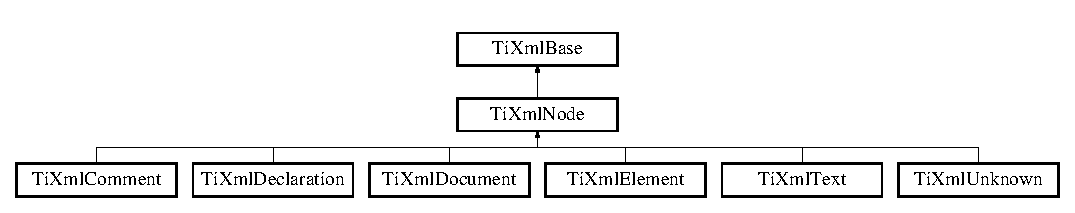
\includegraphics[height=2.41379cm]{classTiXmlNode}
\end{center}
\end{figure}


\subsection{Detailed Description}
The parent class for everything in the Document Object Model. (Except for attributes). Nodes have siblings, a parent, and children. A node can be in a document, or stand on its own. The type of a \doxyref{TiXmlNode}{p.}{classTiXmlNode} can be queried, and it can be cast to its more defined type. \subsection*{Public Types}
\begin{CompactItemize}
\item 
enum {\bf NodeType} \{ \par
{\bf DOCUMENT}, 
{\bf ELEMENT}, 
{\bf COMMENT}, 
{\bf UNKNOWN}, 
\par
{\bf TEXT}, 
{\bf DECLARATION}, 
{\bf TYPECOUNT}
 \}
\end{CompactItemize}
\subsection*{Public Member Functions}
\begin{CompactItemize}
\item 
virtual {\bf $\sim$TiXmlNode} ()
\item 
const char $\ast$ {\bf Value} () const 
\item 
const TIXML\_\-STRING \& {\bf ValueTStr} () const 
\item 
void {\bf SetValue} (const char $\ast$\_\-value)
\item 
void {\bf Clear} ()
\begin{CompactList}\small\item\em Delete all the children of this node. Does not affect 'this'. \item\end{CompactList}\item 
{\bf TiXmlNode} $\ast$ {\bf Parent} ()
\begin{CompactList}\small\item\em One step up the DOM. \item\end{CompactList}\item 
const {\bf TiXmlNode} $\ast$ {\bf Parent} () const 
\item 
const {\bf TiXmlNode} $\ast$ {\bf FirstChild} () const 
\begin{CompactList}\small\item\em The first child of this node. Will be null if there are no children. \item\end{CompactList}\item 
{\bf TiXmlNode} $\ast$ {\bf FirstChild} ()
\item 
const {\bf TiXmlNode} $\ast$ {\bf FirstChild} (const char $\ast${\bf value}) const 
\item 
{\bf TiXmlNode} $\ast$ {\bf FirstChild} (const char $\ast$\_\-value)
\begin{CompactList}\small\item\em The first child of this node with the matching 'value'. Will be null if none found. \item\end{CompactList}\item 
const {\bf TiXmlNode} $\ast$ {\bf LastChild} () const 
\item 
{\bf TiXmlNode} $\ast$ {\bf LastChild} ()
\begin{CompactList}\small\item\em The last child of this node. Will be null if there are no children. \item\end{CompactList}\item 
const {\bf TiXmlNode} $\ast$ {\bf LastChild} (const char $\ast${\bf value}) const 
\item 
{\bf TiXmlNode} $\ast$ {\bf LastChild} (const char $\ast$\_\-value)
\begin{CompactList}\small\item\em The last child of this node matching 'value'. Will be null if there are no children. \item\end{CompactList}\item 
const {\bf TiXmlNode} $\ast$ {\bf IterateChildren} (const {\bf TiXmlNode} $\ast$previous) const 
\item 
{\bf TiXmlNode} $\ast$ {\bf IterateChildren} (const {\bf TiXmlNode} $\ast$previous)
\item 
const {\bf TiXmlNode} $\ast$ {\bf IterateChildren} (const char $\ast${\bf value}, const {\bf TiXmlNode} $\ast$previous) const 
\begin{CompactList}\small\item\em This flavor of IterateChildren searches for children with a particular 'value'. \item\end{CompactList}\item 
{\bf TiXmlNode} $\ast$ {\bf IterateChildren} (const char $\ast$\_\-value, const {\bf TiXmlNode} $\ast$previous)
\item 
{\bf TiXmlNode} $\ast$ {\bf InsertEndChild} (const {\bf TiXmlNode} \&addThis)
\item 
{\bf TiXmlNode} $\ast$ {\bf LinkEndChild} ({\bf TiXmlNode} $\ast$addThis)
\item 
{\bf TiXmlNode} $\ast$ {\bf InsertBeforeChild} ({\bf TiXmlNode} $\ast$beforeThis, const {\bf TiXmlNode} \&addThis)
\item 
{\bf TiXmlNode} $\ast$ {\bf InsertAfterChild} ({\bf TiXmlNode} $\ast$afterThis, const {\bf TiXmlNode} \&addThis)
\item 
{\bf TiXmlNode} $\ast$ {\bf ReplaceChild} ({\bf TiXmlNode} $\ast$replaceThis, const {\bf TiXmlNode} \&withThis)
\item 
bool {\bf RemoveChild} ({\bf TiXmlNode} $\ast$removeThis)
\begin{CompactList}\small\item\em Delete a child of this node. \item\end{CompactList}\item 
const {\bf TiXmlNode} $\ast$ {\bf PreviousSibling} () const 
\begin{CompactList}\small\item\em Navigate to a sibling node. \item\end{CompactList}\item 
{\bf TiXmlNode} $\ast$ {\bf PreviousSibling} ()
\item 
const {\bf TiXmlNode} $\ast$ {\bf PreviousSibling} (const char $\ast$) const 
\begin{CompactList}\small\item\em Navigate to a sibling node. \item\end{CompactList}\item 
{\bf TiXmlNode} $\ast$ {\bf PreviousSibling} (const char $\ast$\_\-prev)
\item 
const {\bf TiXmlNode} $\ast$ {\bf NextSibling} () const 
\begin{CompactList}\small\item\em Navigate to a sibling node. \item\end{CompactList}\item 
{\bf TiXmlNode} $\ast$ {\bf NextSibling} ()
\item 
const {\bf TiXmlNode} $\ast$ {\bf NextSibling} (const char $\ast$) const 
\begin{CompactList}\small\item\em Navigate to a sibling node with the given 'value'. \item\end{CompactList}\item 
{\bf TiXmlNode} $\ast$ {\bf NextSibling} (const char $\ast$\_\-next)
\item 
const {\bf TiXmlElement} $\ast$ {\bf NextSiblingElement} () const 
\item 
{\bf TiXmlElement} $\ast$ {\bf NextSiblingElement} ()
\item 
const {\bf TiXmlElement} $\ast$ {\bf NextSiblingElement} (const char $\ast$) const 
\item 
{\bf TiXmlElement} $\ast$ {\bf NextSiblingElement} (const char $\ast$\_\-next)
\item 
const {\bf TiXmlElement} $\ast$ {\bf FirstChildElement} () const 
\begin{CompactList}\small\item\em Convenience function to get through elements. \item\end{CompactList}\item 
{\bf TiXmlElement} $\ast$ {\bf FirstChildElement} ()
\item 
const {\bf TiXmlElement} $\ast$ {\bf FirstChildElement} (const char $\ast$\_\-value) const 
\begin{CompactList}\small\item\em Convenience function to get through elements. \item\end{CompactList}\item 
{\bf TiXmlElement} $\ast$ {\bf FirstChildElement} (const char $\ast$\_\-value)
\item 
int {\bf Type} () const 
\item 
const {\bf TiXmlDocument} $\ast$ {\bf GetDocument} () const 
\item 
{\bf TiXmlDocument} $\ast$ {\bf GetDocument} ()
\item 
bool {\bf NoChildren} () const 
\begin{CompactList}\small\item\em Returns true if this node has no children. \item\end{CompactList}\item 
virtual const {\bf TiXmlDocument} $\ast$ {\bf ToDocument} () const 
\begin{CompactList}\small\item\em Cast to a more defined type. Will return null if not of the requested type. \item\end{CompactList}\item 
virtual const {\bf TiXmlElement} $\ast$ {\bf ToElement} () const 
\begin{CompactList}\small\item\em Cast to a more defined type. Will return null if not of the requested type. \item\end{CompactList}\item 
virtual const {\bf TiXmlComment} $\ast$ {\bf ToComment} () const 
\begin{CompactList}\small\item\em Cast to a more defined type. Will return null if not of the requested type. \item\end{CompactList}\item 
virtual const {\bf TiXmlUnknown} $\ast$ {\bf ToUnknown} () const 
\begin{CompactList}\small\item\em Cast to a more defined type. Will return null if not of the requested type. \item\end{CompactList}\item 
virtual const {\bf TiXmlText} $\ast$ {\bf ToText} () const 
\begin{CompactList}\small\item\em Cast to a more defined type. Will return null if not of the requested type. \item\end{CompactList}\item 
virtual const {\bf TiXmlDeclaration} $\ast$ {\bf ToDeclaration} () const 
\begin{CompactList}\small\item\em Cast to a more defined type. Will return null if not of the requested type. \item\end{CompactList}\item 
virtual {\bf TiXmlDocument} $\ast$ {\bf ToDocument} ()
\begin{CompactList}\small\item\em Cast to a more defined type. Will return null if not of the requested type. \item\end{CompactList}\item 
virtual {\bf TiXmlElement} $\ast$ {\bf ToElement} ()
\begin{CompactList}\small\item\em Cast to a more defined type. Will return null if not of the requested type. \item\end{CompactList}\item 
virtual {\bf TiXmlComment} $\ast$ {\bf ToComment} ()
\begin{CompactList}\small\item\em Cast to a more defined type. Will return null if not of the requested type. \item\end{CompactList}\item 
virtual {\bf TiXmlUnknown} $\ast$ {\bf ToUnknown} ()
\begin{CompactList}\small\item\em Cast to a more defined type. Will return null if not of the requested type. \item\end{CompactList}\item 
virtual {\bf TiXmlText} $\ast$ {\bf ToText} ()
\begin{CompactList}\small\item\em Cast to a more defined type. Will return null if not of the requested type. \item\end{CompactList}\item 
virtual {\bf TiXmlDeclaration} $\ast$ {\bf ToDeclaration} ()
\begin{CompactList}\small\item\em Cast to a more defined type. Will return null if not of the requested type. \item\end{CompactList}\item 
virtual {\bf TiXmlNode} $\ast$ {\bf Clone} () const =0
\item 
virtual bool {\bf Accept} ({\bf TiXmlVisitor} $\ast$visitor) const =0
\end{CompactItemize}
\subsection*{Protected Member Functions}
\begin{CompactItemize}
\item 
{\bf TiXmlNode} ({\bf NodeType} \_\-type)
\item 
void {\bf CopyTo} ({\bf TiXmlNode} $\ast$target) const 
\item 
{\bf TiXmlNode} $\ast$ {\bf Identify} (const char $\ast$start, {\bf TiXmlEncoding} encoding)
\end{CompactItemize}
\subsection*{Protected Attributes}
\begin{CompactItemize}
\item 
{\bf TiXmlNode} $\ast$ {\bf parent}
\item 
{\bf NodeType} {\bf type}
\item 
{\bf TiXmlNode} $\ast$ {\bf firstChild}
\item 
{\bf TiXmlNode} $\ast$ {\bf lastChild}
\item 
TIXML\_\-STRING {\bf value}
\item 
{\bf TiXmlNode} $\ast$ {\bf prev}
\item 
{\bf TiXmlNode} $\ast$ {\bf next}
\end{CompactItemize}
\subsection*{Friends}
\begin{CompactItemize}
\item 
class {\bf TiXmlDocument}
\item 
class {\bf TiXmlElement}
\end{CompactItemize}


\subsection{Member Enumeration Documentation}
\index{TiXmlNode@{TiXmlNode}!NodeType@{NodeType}}
\index{NodeType@{NodeType}!TiXmlNode@{TiXmlNode}}
\subsubsection[NodeType]{\setlength{\rightskip}{0pt plus 5cm}enum {\bf TiXmlNode::NodeType}}\label{classTiXmlNode_836eded4920ab9e9ef28496f48cd95a2}


The types of XML nodes supported by TinyXml. (All the unsupported types are picked up by UNKNOWN.) \begin{Desc}
\item[Enumerator: ]\par
\begin{description}
\index{DOCUMENT@{DOCUMENT}!TiXmlNode@{TiXmlNode}}\index{TiXmlNode@{TiXmlNode}!DOCUMENT@{DOCUMENT}}\item[{\em 
DOCUMENT\label{classTiXmlNode_836eded4920ab9e9ef28496f48cd95a231b8d14e0558445bb40e36a532b24127}
}]\index{ELEMENT@{ELEMENT}!TiXmlNode@{TiXmlNode}}\index{TiXmlNode@{TiXmlNode}!ELEMENT@{ELEMENT}}\item[{\em 
ELEMENT\label{classTiXmlNode_836eded4920ab9e9ef28496f48cd95a2af2344bcea122ef52d47c4dcc357f070}
}]\index{COMMENT@{COMMENT}!TiXmlNode@{TiXmlNode}}\index{TiXmlNode@{TiXmlNode}!COMMENT@{COMMENT}}\item[{\em 
COMMENT\label{classTiXmlNode_836eded4920ab9e9ef28496f48cd95a27737f35757c7152ca4f612d449ea0e4b}
}]\index{UNKNOWN@{UNKNOWN}!TiXmlNode@{TiXmlNode}}\index{TiXmlNode@{TiXmlNode}!UNKNOWN@{UNKNOWN}}\item[{\em 
UNKNOWN\label{classTiXmlNode_836eded4920ab9e9ef28496f48cd95a2f521ee2fb1e05705776b28fc55a70037}
}]\index{TEXT@{TEXT}!TiXmlNode@{TiXmlNode}}\index{TiXmlNode@{TiXmlNode}!TEXT@{TEXT}}\item[{\em 
TEXT\label{classTiXmlNode_836eded4920ab9e9ef28496f48cd95a2672617f36c5606a966ac378e6ddc0fd8}
}]\index{DECLARATION@{DECLARATION}!TiXmlNode@{TiXmlNode}}\index{TiXmlNode@{TiXmlNode}!DECLARATION@{DECLARATION}}\item[{\em 
DECLARATION\label{classTiXmlNode_836eded4920ab9e9ef28496f48cd95a2c02445686c2b72d11385002b3466c28b}
}]\index{TYPECOUNT@{TYPECOUNT}!TiXmlNode@{TiXmlNode}}\index{TiXmlNode@{TiXmlNode}!TYPECOUNT@{TYPECOUNT}}\item[{\em 
TYPECOUNT\label{classTiXmlNode_836eded4920ab9e9ef28496f48cd95a28334037fb3fe05c67d6110975b38a8bf}
}]\end{description}
\end{Desc}



\subsection{Constructor \& Destructor Documentation}
\index{TiXmlNode@{TiXmlNode}!$\sim$TiXmlNode@{$\sim$TiXmlNode}}
\index{$\sim$TiXmlNode@{$\sim$TiXmlNode}!TiXmlNode@{TiXmlNode}}
\subsubsection[$\sim$TiXmlNode]{\setlength{\rightskip}{0pt plus 5cm}TiXmlNode::$\sim$TiXmlNode ()\hspace{0.3cm}{\tt  [virtual]}}\label{classTiXmlNode_027a76cccd359c831ee4024b58c49625}




References firstChild, and next.\index{TiXmlNode@{TiXmlNode}!TiXmlNode@{TiXmlNode}}
\index{TiXmlNode@{TiXmlNode}!TiXmlNode@{TiXmlNode}}
\subsubsection[TiXmlNode]{\setlength{\rightskip}{0pt plus 5cm}TiXmlNode::TiXmlNode ({\bf NodeType} {\em \_\-type})\hspace{0.3cm}{\tt  [protected]}}\label{classTiXmlNode_3f46721695868667113c7487ff123f20}




References firstChild, lastChild, next, parent, prev, and type.

\subsection{Member Function Documentation}
\index{TiXmlNode@{TiXmlNode}!Value@{Value}}
\index{Value@{Value}!TiXmlNode@{TiXmlNode}}
\subsubsection[Value]{\setlength{\rightskip}{0pt plus 5cm}const char$\ast$ TiXmlNode::Value () const\hspace{0.3cm}{\tt  [inline]}}\label{classTiXmlNode_77943eb90d12c2892b1337a9f5918b41}


The meaning of 'value' changes for the specific type of \doxyref{TiXmlNode}{p.}{classTiXmlNode}. 

\footnotesize\begin{verbatim}
		Document:	filename of the xml file
		Element:	name of the element
		Comment:	the comment text
		Unknown:	the tag contents
		Text:		the text string
		\end{verbatim}
\normalsize


The subclasses will wrap this function. 

References value.

Referenced by TiXmlElement::Clone(), FirstChild(), TiXmlElement::GetText(), LastChild(), TiXmlDocument::LoadFile(), NextSibling(), PreviousSibling(), TiXmlDocument::SaveFile(), TiXmlPrinter::Visit(), TiXmlPrinter::VisitEnter(), and TiXmlPrinter::VisitExit().\index{TiXmlNode@{TiXmlNode}!ValueTStr@{ValueTStr}}
\index{ValueTStr@{ValueTStr}!TiXmlNode@{TiXmlNode}}
\subsubsection[ValueTStr]{\setlength{\rightskip}{0pt plus 5cm}const TIXML\_\-STRING\& TiXmlNode::ValueTStr () const\hspace{0.3cm}{\tt  [inline]}}\label{classTiXmlNode_83ece13d2ea66dac66e0b21332229239}




References value.

Referenced by TiXmlPrinter::Visit().\index{TiXmlNode@{TiXmlNode}!SetValue@{SetValue}}
\index{SetValue@{SetValue}!TiXmlNode@{TiXmlNode}}
\subsubsection[SetValue]{\setlength{\rightskip}{0pt plus 5cm}void TiXmlNode::SetValue (const char $\ast$ {\em \_\-value})\hspace{0.3cm}{\tt  [inline]}}\label{classTiXmlNode_2a38329ca5d3f28f98ce932b8299ae90}


Changes the value of the node. Defined as: 

\footnotesize\begin{verbatim}
		Document:	filename of the xml file
		Element:	name of the element
		Comment:	the comment text
		Unknown:	the tag contents
		Text:		the text string
		\end{verbatim}
\normalsize
 

References value.

Referenced by CopyTo(), TiXmlComment::TiXmlComment(), and TiXmlText::TiXmlText().\index{TiXmlNode@{TiXmlNode}!Clear@{Clear}}
\index{Clear@{Clear}!TiXmlNode@{TiXmlNode}}
\subsubsection[Clear]{\setlength{\rightskip}{0pt plus 5cm}void TiXmlNode::Clear ()}\label{classTiXmlNode_708e7f953df61d4d2d12f73171550a4b}


Delete all the children of this node. Does not affect 'this'. 



References firstChild, lastChild, and next.

Referenced by TiXmlElement::ClearThis(), TiXmlDocument::LoadFile(), TiXmlDeclaration::operator=(), TiXmlComment::operator=(), and TiXmlDocument::operator=().\index{TiXmlNode@{TiXmlNode}!Parent@{Parent}}
\index{Parent@{Parent}!TiXmlNode@{TiXmlNode}}
\subsubsection[Parent]{\setlength{\rightskip}{0pt plus 5cm}{\bf TiXmlNode}$\ast$ TiXmlNode::Parent ()\hspace{0.3cm}{\tt  [inline]}}\label{classTiXmlNode_b643043132ffd794f8602685d34a982e}


One step up the DOM. 



References parent.\index{TiXmlNode@{TiXmlNode}!Parent@{Parent}}
\index{Parent@{Parent}!TiXmlNode@{TiXmlNode}}
\subsubsection[Parent]{\setlength{\rightskip}{0pt plus 5cm}const {\bf TiXmlNode}$\ast$ TiXmlNode::Parent () const\hspace{0.3cm}{\tt  [inline]}}\label{classTiXmlNode_78878709e53066f06eb4fcbcdd3a5260}




References parent.\index{TiXmlNode@{TiXmlNode}!FirstChild@{FirstChild}}
\index{FirstChild@{FirstChild}!TiXmlNode@{TiXmlNode}}
\subsubsection[FirstChild]{\setlength{\rightskip}{0pt plus 5cm}const {\bf TiXmlNode}$\ast$ TiXmlNode::FirstChild () const\hspace{0.3cm}{\tt  [inline]}}\label{classTiXmlNode_44c8eee26bbe2d1b2762038df9dde2f0}


The first child of this node. Will be null if there are no children. 



References firstChild.

Referenced by TiXmlDocument::Accept(), TiXmlElement::Accept(), TiXmlHandle::Child(), TiXmlHandle::FirstChild(), FirstChildElement(), TiXmlElement::GetText(), IterateChildren(), TiXmlDocument::Print(), TiXmlPrinter::VisitEnter(), and TiXmlPrinter::VisitExit().\index{TiXmlNode@{TiXmlNode}!FirstChild@{FirstChild}}
\index{FirstChild@{FirstChild}!TiXmlNode@{TiXmlNode}}
\subsubsection[FirstChild]{\setlength{\rightskip}{0pt plus 5cm}{\bf TiXmlNode}$\ast$ TiXmlNode::FirstChild ()\hspace{0.3cm}{\tt  [inline]}}\label{classTiXmlNode_5e97d69b7c0ebd27fb7286be56559b77}




References firstChild.\index{TiXmlNode@{TiXmlNode}!FirstChild@{FirstChild}}
\index{FirstChild@{FirstChild}!TiXmlNode@{TiXmlNode}}
\subsubsection[FirstChild]{\setlength{\rightskip}{0pt plus 5cm}const {\bf TiXmlNode} $\ast$ TiXmlNode::FirstChild (const char $\ast$ {\em value}) const}\label{classTiXmlNode_b5f722624113c8203227de4f56576d31}


The first child of this node with the matching 'value'. Will be null if none found. 

References firstChild, next, and Value().\index{TiXmlNode@{TiXmlNode}!FirstChild@{FirstChild}}
\index{FirstChild@{FirstChild}!TiXmlNode@{TiXmlNode}}
\subsubsection[FirstChild]{\setlength{\rightskip}{0pt plus 5cm}{\bf TiXmlNode}$\ast$ TiXmlNode::FirstChild (const char $\ast$ {\em \_\-value})\hspace{0.3cm}{\tt  [inline]}}\label{classTiXmlNode_bc8bf32be6419ec453a731868de19554}


The first child of this node with the matching 'value'. Will be null if none found. 

\index{TiXmlNode@{TiXmlNode}!LastChild@{LastChild}}
\index{LastChild@{LastChild}!TiXmlNode@{TiXmlNode}}
\subsubsection[LastChild]{\setlength{\rightskip}{0pt plus 5cm}const {\bf TiXmlNode}$\ast$ TiXmlNode::LastChild () const\hspace{0.3cm}{\tt  [inline]}}\label{classTiXmlNode_6d671107e00cca1d28cb2d7f3a87a21e}




References lastChild.

Referenced by TiXmlPrinter::VisitEnter().\index{TiXmlNode@{TiXmlNode}!LastChild@{LastChild}}
\index{LastChild@{LastChild}!TiXmlNode@{TiXmlNode}}
\subsubsection[LastChild]{\setlength{\rightskip}{0pt plus 5cm}{\bf TiXmlNode}$\ast$ TiXmlNode::LastChild ()\hspace{0.3cm}{\tt  [inline]}}\label{classTiXmlNode_6432d2b2495f6caf9cb4278df706a031}


The last child of this node. Will be null if there are no children. 



References lastChild.\index{TiXmlNode@{TiXmlNode}!LastChild@{LastChild}}
\index{LastChild@{LastChild}!TiXmlNode@{TiXmlNode}}
\subsubsection[LastChild]{\setlength{\rightskip}{0pt plus 5cm}const {\bf TiXmlNode} $\ast$ TiXmlNode::LastChild (const char $\ast$ {\em value}) const}\label{classTiXmlNode_cdd3fdc436aa7433023310a041e5e63f}




References lastChild, prev, and Value().\index{TiXmlNode@{TiXmlNode}!LastChild@{LastChild}}
\index{LastChild@{LastChild}!TiXmlNode@{TiXmlNode}}
\subsubsection[LastChild]{\setlength{\rightskip}{0pt plus 5cm}{\bf TiXmlNode}$\ast$ TiXmlNode::LastChild (const char $\ast$ {\em \_\-value})\hspace{0.3cm}{\tt  [inline]}}\label{classTiXmlNode_bad5bf1059c48127b958711ef89e8e5d}


The last child of this node matching 'value'. Will be null if there are no children. 

\index{TiXmlNode@{TiXmlNode}!IterateChildren@{IterateChildren}}
\index{IterateChildren@{IterateChildren}!TiXmlNode@{TiXmlNode}}
\subsubsection[IterateChildren]{\setlength{\rightskip}{0pt plus 5cm}const {\bf TiXmlNode} $\ast$ TiXmlNode::IterateChildren (const {\bf TiXmlNode} $\ast$ {\em previous}) const}\label{classTiXmlNode_aef7ac3978c4bb1cc8a24ffae7bced75}


An alternate way to walk the children of a node. One way to iterate over nodes is: 

\footnotesize\begin{verbatim}
			for( child = parent->FirstChild(); child; child = child->NextSibling() )
		\end{verbatim}
\normalsize


IterateChildren does the same thing with the syntax: 

\footnotesize\begin{verbatim}
			child = 0;
			while( child = parent->IterateChildren( child ) )
		\end{verbatim}
\normalsize


IterateChildren takes the previous child as input and finds the next one. If the previous child is null, it returns the first. IterateChildren will return null when done. 

References FirstChild(), NextSibling(), and parent.\index{TiXmlNode@{TiXmlNode}!IterateChildren@{IterateChildren}}
\index{IterateChildren@{IterateChildren}!TiXmlNode@{TiXmlNode}}
\subsubsection[IterateChildren]{\setlength{\rightskip}{0pt plus 5cm}{\bf TiXmlNode}$\ast$ TiXmlNode::IterateChildren (const {\bf TiXmlNode} $\ast$ {\em previous})\hspace{0.3cm}{\tt  [inline]}}\label{classTiXmlNode_2358e747118fdbf0e467b1e4f7d03de1}


\index{TiXmlNode@{TiXmlNode}!IterateChildren@{IterateChildren}}
\index{IterateChildren@{IterateChildren}!TiXmlNode@{TiXmlNode}}
\subsubsection[IterateChildren]{\setlength{\rightskip}{0pt plus 5cm}const {\bf TiXmlNode} $\ast$ TiXmlNode::IterateChildren (const char $\ast$ {\em value}, \/  const {\bf TiXmlNode} $\ast$ {\em previous}) const}\label{classTiXmlNode_f2b86dbe25d3d26fa48180edc5e2a9fc}


This flavor of IterateChildren searches for children with a particular 'value'. 



References FirstChild(), NextSibling(), and parent.\index{TiXmlNode@{TiXmlNode}!IterateChildren@{IterateChildren}}
\index{IterateChildren@{IterateChildren}!TiXmlNode@{TiXmlNode}}
\subsubsection[IterateChildren]{\setlength{\rightskip}{0pt plus 5cm}{\bf TiXmlNode}$\ast$ TiXmlNode::IterateChildren (const char $\ast$ {\em \_\-value}, \/  const {\bf TiXmlNode} $\ast$ {\em previous})\hspace{0.3cm}{\tt  [inline]}}\label{classTiXmlNode_67ba8275e533e6f76340236c42ea0aea}


\index{TiXmlNode@{TiXmlNode}!InsertEndChild@{InsertEndChild}}
\index{InsertEndChild@{InsertEndChild}!TiXmlNode@{TiXmlNode}}
\subsubsection[InsertEndChild]{\setlength{\rightskip}{0pt plus 5cm}{\bf TiXmlNode} $\ast$ TiXmlNode::InsertEndChild (const {\bf TiXmlNode} \& {\em addThis})}\label{classTiXmlNode_f287a913ce46d8dbf7ef24fec69bbaf0}


Add a new node related to this. Adds a child past the LastChild. Returns a pointer to the new object or NULL if an error occured. 

References Clone(), DOCUMENT, GetDocument(), LinkEndChild(), TiXmlDocument::SetError(), TIXML\_\-ENCODING\_\-UNKNOWN, TiXmlBase::TIXML\_\-ERROR\_\-DOCUMENT\_\-TOP\_\-ONLY, and Type().\index{TiXmlNode@{TiXmlNode}!LinkEndChild@{LinkEndChild}}
\index{LinkEndChild@{LinkEndChild}!TiXmlNode@{TiXmlNode}}
\subsubsection[LinkEndChild]{\setlength{\rightskip}{0pt plus 5cm}{\bf TiXmlNode} $\ast$ TiXmlNode::LinkEndChild ({\bf TiXmlNode} $\ast$ {\em addThis})}\label{classTiXmlNode_1a881212554b759865f6cac79a851d38}


Add a new node related to this. Adds a child past the LastChild.

NOTE: the node to be added is passed by pointer, and will be henceforth owned (and deleted) by tinyXml. This method is efficient and avoids an extra copy, but should be used with care as it uses a different memory model than the other insert functions.

\begin{Desc}
\item[See also:]\doxyref{InsertEndChild}{p.}{classTiXmlNode_f287a913ce46d8dbf7ef24fec69bbaf0} \end{Desc}


References DOCUMENT, firstChild, GetDocument(), lastChild, next, parent, prev, TiXmlDocument::SetError(), TIXML\_\-ENCODING\_\-UNKNOWN, TiXmlBase::TIXML\_\-ERROR\_\-DOCUMENT\_\-TOP\_\-ONLY, and Type().

Referenced by TiXmlElement::CopyTo(), InsertEndChild(), TiXmlDocument::Parse(), and TiXmlElement::ReadValue().\index{TiXmlNode@{TiXmlNode}!InsertBeforeChild@{InsertBeforeChild}}
\index{InsertBeforeChild@{InsertBeforeChild}!TiXmlNode@{TiXmlNode}}
\subsubsection[InsertBeforeChild]{\setlength{\rightskip}{0pt plus 5cm}{\bf TiXmlNode} $\ast$ TiXmlNode::InsertBeforeChild ({\bf TiXmlNode} $\ast$ {\em beforeThis}, \/  const {\bf TiXmlNode} \& {\em addThis})}\label{classTiXmlNode_71e54e393336382bc9875f64aab5cb15}


Add a new node related to this. Adds a child before the specified child. Returns a pointer to the new object or NULL if an error occured. 

References Clone(), DOCUMENT, firstChild, GetDocument(), next, parent, prev, TiXmlDocument::SetError(), TIXML\_\-ENCODING\_\-UNKNOWN, TiXmlBase::TIXML\_\-ERROR\_\-DOCUMENT\_\-TOP\_\-ONLY, and Type().\index{TiXmlNode@{TiXmlNode}!InsertAfterChild@{InsertAfterChild}}
\index{InsertAfterChild@{InsertAfterChild}!TiXmlNode@{TiXmlNode}}
\subsubsection[InsertAfterChild]{\setlength{\rightskip}{0pt plus 5cm}{\bf TiXmlNode} $\ast$ TiXmlNode::InsertAfterChild ({\bf TiXmlNode} $\ast$ {\em afterThis}, \/  const {\bf TiXmlNode} \& {\em addThis})}\label{classTiXmlNode_274db3292218202805c093f66a964cb5}


Add a new node related to this. Adds a child after the specified child. Returns a pointer to the new object or NULL if an error occured. 

References Clone(), DOCUMENT, GetDocument(), lastChild, next, parent, prev, TiXmlDocument::SetError(), TIXML\_\-ENCODING\_\-UNKNOWN, TiXmlBase::TIXML\_\-ERROR\_\-DOCUMENT\_\-TOP\_\-ONLY, and Type().\index{TiXmlNode@{TiXmlNode}!ReplaceChild@{ReplaceChild}}
\index{ReplaceChild@{ReplaceChild}!TiXmlNode@{TiXmlNode}}
\subsubsection[ReplaceChild]{\setlength{\rightskip}{0pt plus 5cm}{\bf TiXmlNode} $\ast$ TiXmlNode::ReplaceChild ({\bf TiXmlNode} $\ast$ {\em replaceThis}, \/  const {\bf TiXmlNode} \& {\em withThis})}\label{classTiXmlNode_543208c2c801c84a213529541e904b9f}


Replace a child of this node. Returns a pointer to the new object or NULL if an error occured. 

References Clone(), firstChild, lastChild, next, parent, and prev.\index{TiXmlNode@{TiXmlNode}!RemoveChild@{RemoveChild}}
\index{RemoveChild@{RemoveChild}!TiXmlNode@{TiXmlNode}}
\subsubsection[RemoveChild]{\setlength{\rightskip}{0pt plus 5cm}bool TiXmlNode::RemoveChild ({\bf TiXmlNode} $\ast$ {\em removeThis})}\label{classTiXmlNode_e19d8510efc90596552f4feeac9a8fbf}


Delete a child of this node. 



References firstChild, lastChild, next, parent, and prev.\index{TiXmlNode@{TiXmlNode}!PreviousSibling@{PreviousSibling}}
\index{PreviousSibling@{PreviousSibling}!TiXmlNode@{TiXmlNode}}
\subsubsection[PreviousSibling]{\setlength{\rightskip}{0pt plus 5cm}const {\bf TiXmlNode}$\ast$ TiXmlNode::PreviousSibling () const\hspace{0.3cm}{\tt  [inline]}}\label{classTiXmlNode_c2cd892768726270e511b2ab32de4d10}


Navigate to a sibling node. 



References prev.\index{TiXmlNode@{TiXmlNode}!PreviousSibling@{PreviousSibling}}
\index{PreviousSibling@{PreviousSibling}!TiXmlNode@{TiXmlNode}}
\subsubsection[PreviousSibling]{\setlength{\rightskip}{0pt plus 5cm}{\bf TiXmlNode}$\ast$ TiXmlNode::PreviousSibling ()\hspace{0.3cm}{\tt  [inline]}}\label{classTiXmlNode_f8c0642ad6ecc03f62953e68896ed1cc}




References prev.\index{TiXmlNode@{TiXmlNode}!PreviousSibling@{PreviousSibling}}
\index{PreviousSibling@{PreviousSibling}!TiXmlNode@{TiXmlNode}}
\subsubsection[PreviousSibling]{\setlength{\rightskip}{0pt plus 5cm}const {\bf TiXmlNode} $\ast$ TiXmlNode::PreviousSibling (const char $\ast$ {\em \_\-value}) const}\label{classTiXmlNode_bbb3b8c1f38fa7b9e52d584a4aeca795}


Navigate to a sibling node. 



References prev, and Value().\index{TiXmlNode@{TiXmlNode}!PreviousSibling@{PreviousSibling}}
\index{PreviousSibling@{PreviousSibling}!TiXmlNode@{TiXmlNode}}
\subsubsection[PreviousSibling]{\setlength{\rightskip}{0pt plus 5cm}{\bf TiXmlNode}$\ast$ TiXmlNode::PreviousSibling (const char $\ast$ {\em \_\-prev})\hspace{0.3cm}{\tt  [inline]}}\label{classTiXmlNode_6c977049207177ef21b51972315c2053}


\index{TiXmlNode@{TiXmlNode}!NextSibling@{NextSibling}}
\index{NextSibling@{NextSibling}!TiXmlNode@{TiXmlNode}}
\subsubsection[NextSibling]{\setlength{\rightskip}{0pt plus 5cm}const {\bf TiXmlNode}$\ast$ TiXmlNode::NextSibling () const\hspace{0.3cm}{\tt  [inline]}}\label{classTiXmlNode_f854baeba384f5fe9859f5aee03b548e}


Navigate to a sibling node. 



References next.

Referenced by TiXmlDocument::Accept(), TiXmlHandle::Child(), TiXmlElement::CopyTo(), FirstChildElement(), IterateChildren(), NextSiblingElement(), TiXmlDocument::Print(), and TiXmlElement::Print().\index{TiXmlNode@{TiXmlNode}!NextSibling@{NextSibling}}
\index{NextSibling@{NextSibling}!TiXmlNode@{TiXmlNode}}
\subsubsection[NextSibling]{\setlength{\rightskip}{0pt plus 5cm}{\bf TiXmlNode}$\ast$ TiXmlNode::NextSibling ()\hspace{0.3cm}{\tt  [inline]}}\label{classTiXmlNode_4d05f7b1d7b470ac6887edd072d4892a}




References next.\index{TiXmlNode@{TiXmlNode}!NextSibling@{NextSibling}}
\index{NextSibling@{NextSibling}!TiXmlNode@{TiXmlNode}}
\subsubsection[NextSibling]{\setlength{\rightskip}{0pt plus 5cm}const {\bf TiXmlNode} $\ast$ TiXmlNode::NextSibling (const char $\ast$ {\em \_\-value}) const}\label{classTiXmlNode_caf9dc17531ac041f602f9ad579573ea}


Navigate to a sibling node with the given 'value'. 



References next, and Value().\index{TiXmlNode@{TiXmlNode}!NextSibling@{NextSibling}}
\index{NextSibling@{NextSibling}!TiXmlNode@{TiXmlNode}}
\subsubsection[NextSibling]{\setlength{\rightskip}{0pt plus 5cm}{\bf TiXmlNode}$\ast$ TiXmlNode::NextSibling (const char $\ast$ {\em \_\-next})\hspace{0.3cm}{\tt  [inline]}}\label{classTiXmlNode_4080bc5cc8a5c139e7cf308669e850fc}


\index{TiXmlNode@{TiXmlNode}!NextSiblingElement@{NextSiblingElement}}
\index{NextSiblingElement@{NextSiblingElement}!TiXmlNode@{TiXmlNode}}
\subsubsection[NextSiblingElement]{\setlength{\rightskip}{0pt plus 5cm}const {\bf TiXmlElement} $\ast$ TiXmlNode::NextSiblingElement () const}\label{classTiXmlNode_7667217e269e0da01d1f82aee94d1a3d}


Convenience function to get through elements. Calls NextSibling and ToElement. Will skip all non-Element nodes. Returns 0 if there is not another element. 

References NextSibling(), and ToElement().

Referenced by TiXmlHandle::ChildElement().\index{TiXmlNode@{TiXmlNode}!NextSiblingElement@{NextSiblingElement}}
\index{NextSiblingElement@{NextSiblingElement}!TiXmlNode@{TiXmlNode}}
\subsubsection[NextSiblingElement]{\setlength{\rightskip}{0pt plus 5cm}{\bf TiXmlElement}$\ast$ TiXmlNode::NextSiblingElement ()\hspace{0.3cm}{\tt  [inline]}}\label{classTiXmlNode_1b211cb5034655a04358e0e2f6fc5010}


\index{TiXmlNode@{TiXmlNode}!NextSiblingElement@{NextSiblingElement}}
\index{NextSiblingElement@{NextSiblingElement}!TiXmlNode@{TiXmlNode}}
\subsubsection[NextSiblingElement]{\setlength{\rightskip}{0pt plus 5cm}const {\bf TiXmlElement} $\ast$ TiXmlNode::NextSiblingElement (const char $\ast$ {\em \_\-value}) const}\label{classTiXmlNode_3d7897999f99cf4870dd59df6331d7ff}


Convenience function to get through elements. Calls NextSibling and ToElement. Will skip all non-Element nodes. Returns 0 if there is not another element. 

References NextSibling(), and ToElement().\index{TiXmlNode@{TiXmlNode}!NextSiblingElement@{NextSiblingElement}}
\index{NextSiblingElement@{NextSiblingElement}!TiXmlNode@{TiXmlNode}}
\subsubsection[NextSiblingElement]{\setlength{\rightskip}{0pt plus 5cm}{\bf TiXmlElement}$\ast$ TiXmlNode::NextSiblingElement (const char $\ast$ {\em \_\-next})\hspace{0.3cm}{\tt  [inline]}}\label{classTiXmlNode_6e1ac6b800e18049bc75e9f8e63a8e5f}


\index{TiXmlNode@{TiXmlNode}!FirstChildElement@{FirstChildElement}}
\index{FirstChildElement@{FirstChildElement}!TiXmlNode@{TiXmlNode}}
\subsubsection[FirstChildElement]{\setlength{\rightskip}{0pt plus 5cm}const {\bf TiXmlElement} $\ast$ TiXmlNode::FirstChildElement () const}\label{classTiXmlNode_b1f8d8e70d88aea4c5efedfe00862d55}


Convenience function to get through elements. 



References FirstChild(), NextSibling(), and ToElement().

Referenced by TiXmlHandle::ChildElement(), TiXmlHandle::FirstChildElement(), and TiXmlDocument::RootElement().\index{TiXmlNode@{TiXmlNode}!FirstChildElement@{FirstChildElement}}
\index{FirstChildElement@{FirstChildElement}!TiXmlNode@{TiXmlNode}}
\subsubsection[FirstChildElement]{\setlength{\rightskip}{0pt plus 5cm}{\bf TiXmlElement}$\ast$ TiXmlNode::FirstChildElement ()\hspace{0.3cm}{\tt  [inline]}}\label{classTiXmlNode_a0fecff1f3866ab33a8a25506e95db1d}


\index{TiXmlNode@{TiXmlNode}!FirstChildElement@{FirstChildElement}}
\index{FirstChildElement@{FirstChildElement}!TiXmlNode@{TiXmlNode}}
\subsubsection[FirstChildElement]{\setlength{\rightskip}{0pt plus 5cm}const {\bf TiXmlElement} $\ast$ TiXmlNode::FirstChildElement (const char $\ast$ {\em \_\-value}) const}\label{classTiXmlNode_0ec361bfef1cf1978d060295f597e0d9}


Convenience function to get through elements. 



References FirstChild(), NextSibling(), and ToElement().\index{TiXmlNode@{TiXmlNode}!FirstChildElement@{FirstChildElement}}
\index{FirstChildElement@{FirstChildElement}!TiXmlNode@{TiXmlNode}}
\subsubsection[FirstChildElement]{\setlength{\rightskip}{0pt plus 5cm}{\bf TiXmlElement}$\ast$ TiXmlNode::FirstChildElement (const char $\ast$ {\em \_\-value})\hspace{0.3cm}{\tt  [inline]}}\label{classTiXmlNode_6936ae323675071808ac4840379e57f5}


\index{TiXmlNode@{TiXmlNode}!Type@{Type}}
\index{Type@{Type}!TiXmlNode@{TiXmlNode}}
\subsubsection[Type]{\setlength{\rightskip}{0pt plus 5cm}int TiXmlNode::Type () const\hspace{0.3cm}{\tt  [inline]}}\label{classTiXmlNode_57b99d5c97d67a42b9752f5210a1ba5e}


Query the type (as an enumerated value, above) of this node. The possible types are: DOCUMENT, ELEMENT, COMMENT, UNKNOWN, TEXT, and DECLARATION. 

References type.

Referenced by InsertAfterChild(), InsertBeforeChild(), InsertEndChild(), and LinkEndChild().\index{TiXmlNode@{TiXmlNode}!GetDocument@{GetDocument}}
\index{GetDocument@{GetDocument}!TiXmlNode@{TiXmlNode}}
\subsubsection[GetDocument]{\setlength{\rightskip}{0pt plus 5cm}const {\bf TiXmlDocument} $\ast$ TiXmlNode::GetDocument () const}\label{classTiXmlNode_a66f4ebcd175204a168ed7c2d7b43071}


Return a pointer to the Document this node lives in. Returns null if not in a document. 

References parent, and ToDocument().

Referenced by Identify(), InsertAfterChild(), InsertBeforeChild(), InsertEndChild(), LinkEndChild(), TiXmlDeclaration::Parse(), TiXmlText::Parse(), TiXmlComment::Parse(), TiXmlUnknown::Parse(), TiXmlElement::Parse(), TiXmlElement::ReadValue(), and TiXmlElement::SetAttribute().\index{TiXmlNode@{TiXmlNode}!GetDocument@{GetDocument}}
\index{GetDocument@{GetDocument}!TiXmlNode@{TiXmlNode}}
\subsubsection[GetDocument]{\setlength{\rightskip}{0pt plus 5cm}{\bf TiXmlDocument}$\ast$ TiXmlNode::GetDocument ()\hspace{0.3cm}{\tt  [inline]}}\label{classTiXmlNode_7b2372c0e7adfb32f5b6902fe49a39b2}


\index{TiXmlNode@{TiXmlNode}!NoChildren@{NoChildren}}
\index{NoChildren@{NoChildren}!TiXmlNode@{TiXmlNode}}
\subsubsection[NoChildren]{\setlength{\rightskip}{0pt plus 5cm}bool TiXmlNode::NoChildren () const\hspace{0.3cm}{\tt  [inline]}}\label{classTiXmlNode_eed21ad30630ef6e7faf096127edc9f3}


Returns true if this node has no children. 



References firstChild.\index{TiXmlNode@{TiXmlNode}!ToDocument@{ToDocument}}
\index{ToDocument@{ToDocument}!TiXmlNode@{TiXmlNode}}
\subsubsection[ToDocument]{\setlength{\rightskip}{0pt plus 5cm}virtual const {\bf TiXmlDocument}$\ast$ TiXmlNode::ToDocument () const\hspace{0.3cm}{\tt  [inline, virtual]}}\label{classTiXmlNode_8a4cda4b15c29f64cff419309aebed08}


Cast to a more defined type. Will return null if not of the requested type. 



Reimplemented in {\bf TiXmlDocument} \doxyref{}{p.}{classTiXmlDocument_1dc977bde3e4fe85a8eb9d88a35ef5a4}.

Referenced by GetDocument().\index{TiXmlNode@{TiXmlNode}!ToElement@{ToElement}}
\index{ToElement@{ToElement}!TiXmlNode@{TiXmlNode}}
\subsubsection[ToElement]{\setlength{\rightskip}{0pt plus 5cm}virtual const {\bf TiXmlElement}$\ast$ TiXmlNode::ToElement () const\hspace{0.3cm}{\tt  [inline, virtual]}}\label{classTiXmlNode_72abed96dc9667ab9e0a2a275301bb1c}


Cast to a more defined type. Will return null if not of the requested type. 



Reimplemented in {\bf TiXmlElement} \doxyref{}{p.}{classTiXmlElement_c5b8d0e25fa23fd9acbb6d146082901c}.

Referenced by FirstChildElement(), and NextSiblingElement().\index{TiXmlNode@{TiXmlNode}!ToComment@{ToComment}}
\index{ToComment@{ToComment}!TiXmlNode@{TiXmlNode}}
\subsubsection[ToComment]{\setlength{\rightskip}{0pt plus 5cm}virtual const {\bf TiXmlComment}$\ast$ TiXmlNode::ToComment () const\hspace{0.3cm}{\tt  [inline, virtual]}}\label{classTiXmlNode_a0a5086f9eaee910bbfdc7f975e26574}


Cast to a more defined type. Will return null if not of the requested type. 



Reimplemented in {\bf TiXmlComment} \doxyref{}{p.}{classTiXmlComment_00fb4215c20a2399ea05ac9b9e7e68a0}.\index{TiXmlNode@{TiXmlNode}!ToUnknown@{ToUnknown}}
\index{ToUnknown@{ToUnknown}!TiXmlNode@{TiXmlNode}}
\subsubsection[ToUnknown]{\setlength{\rightskip}{0pt plus 5cm}virtual const {\bf TiXmlUnknown}$\ast$ TiXmlNode::ToUnknown () const\hspace{0.3cm}{\tt  [inline, virtual]}}\label{classTiXmlNode_fd7205cf31d7a376929f8a36930627a2}


Cast to a more defined type. Will return null if not of the requested type. 



Reimplemented in {\bf TiXmlUnknown} \doxyref{}{p.}{classTiXmlUnknown_b0313e5fe77987d746ac1a97a254419d}.\index{TiXmlNode@{TiXmlNode}!ToText@{ToText}}
\index{ToText@{ToText}!TiXmlNode@{TiXmlNode}}
\subsubsection[ToText]{\setlength{\rightskip}{0pt plus 5cm}virtual const {\bf TiXmlText}$\ast$ TiXmlNode::ToText () const\hspace{0.3cm}{\tt  [inline, virtual]}}\label{classTiXmlNode_95a46a52c525992d6b4ee08beb14cd69}


Cast to a more defined type. Will return null if not of the requested type. 



Reimplemented in {\bf TiXmlText} \doxyref{}{p.}{classTiXmlText_895bf34ffad17f7439ab2a52b9651648}.

Referenced by TiXmlElement::GetText(), TiXmlElement::Print(), and TiXmlPrinter::VisitEnter().\index{TiXmlNode@{TiXmlNode}!ToDeclaration@{ToDeclaration}}
\index{ToDeclaration@{ToDeclaration}!TiXmlNode@{TiXmlNode}}
\subsubsection[ToDeclaration]{\setlength{\rightskip}{0pt plus 5cm}virtual const {\bf TiXmlDeclaration}$\ast$ TiXmlNode::ToDeclaration () const\hspace{0.3cm}{\tt  [inline, virtual]}}\label{classTiXmlNode_9f43e6984fc7d4afd6eb32714c6b7b72}


Cast to a more defined type. Will return null if not of the requested type. 



Reimplemented in {\bf TiXmlDeclaration} \doxyref{}{p.}{classTiXmlDeclaration_1e085d3fefd1dbf5ccdbff729931a967}.

Referenced by TiXmlDocument::Parse().\index{TiXmlNode@{TiXmlNode}!ToDocument@{ToDocument}}
\index{ToDocument@{ToDocument}!TiXmlNode@{TiXmlNode}}
\subsubsection[ToDocument]{\setlength{\rightskip}{0pt plus 5cm}virtual {\bf TiXmlDocument}$\ast$ TiXmlNode::ToDocument ()\hspace{0.3cm}{\tt  [inline, virtual]}}\label{classTiXmlNode_6a4c8ac28ee7a745d059db6691e03bae}


Cast to a more defined type. Will return null if not of the requested type. 



Reimplemented in {\bf TiXmlDocument} \doxyref{}{p.}{classTiXmlDocument_1025d942a1f328fd742d545e37efdd42}.\index{TiXmlNode@{TiXmlNode}!ToElement@{ToElement}}
\index{ToElement@{ToElement}!TiXmlNode@{TiXmlNode}}
\subsubsection[ToElement]{\setlength{\rightskip}{0pt plus 5cm}virtual {\bf TiXmlElement}$\ast$ TiXmlNode::ToElement ()\hspace{0.3cm}{\tt  [inline, virtual]}}\label{classTiXmlNode_a65d000223187d22a4dcebd7479e9ebc}


Cast to a more defined type. Will return null if not of the requested type. 



Reimplemented in {\bf TiXmlElement} \doxyref{}{p.}{classTiXmlElement_9def86337ea7a755eb41cac980f60c7a}.\index{TiXmlNode@{TiXmlNode}!ToComment@{ToComment}}
\index{ToComment@{ToComment}!TiXmlNode@{TiXmlNode}}
\subsubsection[ToComment]{\setlength{\rightskip}{0pt plus 5cm}virtual {\bf TiXmlComment}$\ast$ TiXmlNode::ToComment ()\hspace{0.3cm}{\tt  [inline, virtual]}}\label{classTiXmlNode_383e06a0787f7063953934867990f849}


Cast to a more defined type. Will return null if not of the requested type. 



Reimplemented in {\bf TiXmlComment} \doxyref{}{p.}{classTiXmlComment_cc7c7e07e13c23f17797d642981511df}.\index{TiXmlNode@{TiXmlNode}!ToUnknown@{ToUnknown}}
\index{ToUnknown@{ToUnknown}!TiXmlNode@{TiXmlNode}}
\subsubsection[ToUnknown]{\setlength{\rightskip}{0pt plus 5cm}virtual {\bf TiXmlUnknown}$\ast$ TiXmlNode::ToUnknown ()\hspace{0.3cm}{\tt  [inline, virtual]}}\label{classTiXmlNode_06de5af852668c7e4af0d09c205f0b0d}


Cast to a more defined type. Will return null if not of the requested type. 



Reimplemented in {\bf TiXmlUnknown} \doxyref{}{p.}{classTiXmlUnknown_67c9fd22940e8c47f706a72cdd2e332c}.\index{TiXmlNode@{TiXmlNode}!ToText@{ToText}}
\index{ToText@{ToText}!TiXmlNode@{TiXmlNode}}
\subsubsection[ToText]{\setlength{\rightskip}{0pt plus 5cm}virtual {\bf TiXmlText}$\ast$ TiXmlNode::ToText ()\hspace{0.3cm}{\tt  [inline, virtual]}}\label{classTiXmlNode_3ddfbcac78fbea041fad57e5c6d60a03}


Cast to a more defined type. Will return null if not of the requested type. 



Reimplemented in {\bf TiXmlText} \doxyref{}{p.}{classTiXmlText_e7c3a8fd3e4dbf6c0c4363a943d72f5b}.\index{TiXmlNode@{TiXmlNode}!ToDeclaration@{ToDeclaration}}
\index{ToDeclaration@{ToDeclaration}!TiXmlNode@{TiXmlNode}}
\subsubsection[ToDeclaration]{\setlength{\rightskip}{0pt plus 5cm}virtual {\bf TiXmlDeclaration}$\ast$ TiXmlNode::ToDeclaration ()\hspace{0.3cm}{\tt  [inline, virtual]}}\label{classTiXmlNode_4027136ca820ff4a636b607231b6a6df}


Cast to a more defined type. Will return null if not of the requested type. 



Reimplemented in {\bf TiXmlDeclaration} \doxyref{}{p.}{classTiXmlDeclaration_6bd3d1daddcaeb9543c24bfd090969ce}.\index{TiXmlNode@{TiXmlNode}!Clone@{Clone}}
\index{Clone@{Clone}!TiXmlNode@{TiXmlNode}}
\subsubsection[Clone]{\setlength{\rightskip}{0pt plus 5cm}virtual {\bf TiXmlNode}$\ast$ TiXmlNode::Clone () const\hspace{0.3cm}{\tt  [pure virtual]}}\label{classTiXmlNode_4508cc3a2d7a98e96a54cc09c37a78a4}


Create an exact duplicate of this node and return it. The memory must be deleted by the caller. 

Implemented in {\bf TiXmlElement} \doxyref{}{p.}{classTiXmlElement_13f6df105ebb1e8dc636e75cc883be32}, {\bf TiXmlComment} \doxyref{}{p.}{classTiXmlComment_4f6590c9c9a2b63a48972655b78eb853}, {\bf TiXmlText} \doxyref{}{p.}{classTiXmlText_dde1869dfb029be50713fbfd8ce4d21f}, {\bf TiXmlDeclaration} \doxyref{}{p.}{classTiXmlDeclaration_ff8231266d735943d8a7514a9c9822b9}, {\bf TiXmlUnknown} \doxyref{}{p.}{classTiXmlUnknown_675c4b2684af35e4c7649b7fd5ae598d}, and {\bf TiXmlDocument} \doxyref{}{p.}{classTiXmlDocument_c9e8f09b23454d953b32d1b65cd1409e}.

Referenced by TiXmlElement::CopyTo(), InsertAfterChild(), InsertBeforeChild(), InsertEndChild(), and ReplaceChild().\index{TiXmlNode@{TiXmlNode}!Accept@{Accept}}
\index{Accept@{Accept}!TiXmlNode@{TiXmlNode}}
\subsubsection[Accept]{\setlength{\rightskip}{0pt plus 5cm}virtual bool TiXmlNode::Accept ({\bf TiXmlVisitor} $\ast$ {\em visitor}) const\hspace{0.3cm}{\tt  [pure virtual]}}\label{classTiXmlNode_cc0f88b7462c6cb73809d410a4f5bb86}


Accept a hierchical visit the nodes in the TinyXML DOM. Every node in the XML tree will be conditionally visited and the host will be called back via the \doxyref{TiXmlVisitor}{p.}{classTiXmlVisitor} interface.

This is essentially a SAX interface for TinyXML. (Note however it doesn't re-parse the XML for the callbacks, so the performance of TinyXML is unchanged by using this interface versus any other.)

The interface has been based on ideas from:

\begin{itemize}
\item {\tt http://www.saxproject.org/}\item {\tt http://c2.com/cgi/wiki?HierarchicalVisitorPattern}\end{itemize}


Which are both good references for \char`\"{}visiting\char`\"{}.

An example of using \doxyref{Accept()}{p.}{classTiXmlNode_cc0f88b7462c6cb73809d410a4f5bb86}: 

\footnotesize\begin{verbatim}
		TiXmlPrinter printer;
		tinyxmlDoc.Accept( &printer );
		const char* xmlcstr = printer.CStr();
		\end{verbatim}
\normalsize
 

Implemented in {\bf TiXmlElement} \doxyref{}{p.}{classTiXmlElement_31ab28cc3b892a69254391d6bbe08df3}, {\bf TiXmlComment} \doxyref{}{p.}{classTiXmlComment_4382de0e50da973f11a23ea5852568bd}, {\bf TiXmlText} \doxyref{}{p.}{classTiXmlText_43b9954ebf679557fac1a4453f337b7c}, {\bf TiXmlDeclaration} \doxyref{}{p.}{classTiXmlDeclaration_b6a6b178161ba9abc2c35058de689864}, {\bf TiXmlUnknown} \doxyref{}{p.}{classTiXmlUnknown_4e54d7482e05a837cf83c925cc683380}, and {\bf TiXmlDocument} \doxyref{}{p.}{classTiXmlDocument_3daab2f472418ef66315750202f762ae}.

Referenced by TiXmlDocument::Accept().\index{TiXmlNode@{TiXmlNode}!CopyTo@{CopyTo}}
\index{CopyTo@{CopyTo}!TiXmlNode@{TiXmlNode}}
\subsubsection[CopyTo]{\setlength{\rightskip}{0pt plus 5cm}void TiXmlNode::CopyTo ({\bf TiXmlNode} $\ast$ {\em target}) const\hspace{0.3cm}{\tt  [protected]}}\label{classTiXmlNode_b6056978923ad8350fb5164af32d8038}




References SetValue(), TiXmlBase::userData, and value.

Referenced by TiXmlUnknown::CopyTo(), TiXmlDeclaration::CopyTo(), TiXmlText::CopyTo(), TiXmlComment::CopyTo(), and TiXmlElement::CopyTo().\index{TiXmlNode@{TiXmlNode}!Identify@{Identify}}
\index{Identify@{Identify}!TiXmlNode@{TiXmlNode}}
\subsubsection[Identify]{\setlength{\rightskip}{0pt plus 5cm}{\bf TiXmlNode} $\ast$ TiXmlNode::Identify (const char $\ast$ {\em start}, \/  {\bf TiXmlEncoding} {\em encoding})\hspace{0.3cm}{\tt  [protected]}}\label{classTiXmlNode_c1e3a8e7578be463b04617786120c2bb}




References GetDocument(), TiXmlBase::IsAlpha(), parent, TiXmlText::SetCDATA(), TiXmlDocument::SetError(), TiXmlBase::SkipWhiteSpace(), TiXmlBase::StringEqual(), TIXML\_\-ENCODING\_\-UNKNOWN, TiXmlBase::TIXML\_\-ERROR\_\-OUT\_\-OF\_\-MEMORY, and TiXmlElement.

Referenced by TiXmlDocument::Parse(), and TiXmlElement::ReadValue().

\subsection{Friends And Related Function Documentation}
\index{TiXmlNode@{TiXmlNode}!TiXmlDocument@{TiXmlDocument}}
\index{TiXmlDocument@{TiXmlDocument}!TiXmlNode@{TiXmlNode}}
\subsubsection[TiXmlDocument]{\setlength{\rightskip}{0pt plus 5cm}friend class {\bf TiXmlDocument}\hspace{0.3cm}{\tt  [friend]}}\label{classTiXmlNode_173617f6dfe902cf484ce5552b950475}




Reimplemented from {\bf TiXmlBase} \doxyref{}{p.}{classTiXmlBase_173617f6dfe902cf484ce5552b950475}.\index{TiXmlNode@{TiXmlNode}!TiXmlElement@{TiXmlElement}}
\index{TiXmlElement@{TiXmlElement}!TiXmlNode@{TiXmlNode}}
\subsubsection[TiXmlElement]{\setlength{\rightskip}{0pt plus 5cm}friend class {\bf TiXmlElement}\hspace{0.3cm}{\tt  [friend]}}\label{classTiXmlNode_b6592e32cb9132be517cc12a70564c4b}




Reimplemented from {\bf TiXmlBase} \doxyref{}{p.}{classTiXmlBase_b6592e32cb9132be517cc12a70564c4b}.

Reimplemented in {\bf TiXmlText} \doxyref{}{p.}{classTiXmlText_b6592e32cb9132be517cc12a70564c4b}.

Referenced by Identify().

\subsection{Member Data Documentation}
\index{TiXmlNode@{TiXmlNode}!parent@{parent}}
\index{parent@{parent}!TiXmlNode@{TiXmlNode}}
\subsubsection[parent]{\setlength{\rightskip}{0pt plus 5cm}{\bf TiXmlNode}$\ast$ {\bf TiXmlNode::parent}\hspace{0.3cm}{\tt  [protected]}}\label{classTiXmlNode_662c4de61244e4fa5bd4e2d8c63143a5}




Referenced by GetDocument(), Identify(), InsertAfterChild(), InsertBeforeChild(), IterateChildren(), LinkEndChild(), Parent(), RemoveChild(), ReplaceChild(), and TiXmlNode().\index{TiXmlNode@{TiXmlNode}!type@{type}}
\index{type@{type}!TiXmlNode@{TiXmlNode}}
\subsubsection[type]{\setlength{\rightskip}{0pt plus 5cm}{\bf NodeType} {\bf TiXmlNode::type}\hspace{0.3cm}{\tt  [protected]}}\label{classTiXmlNode_2619c6379181c16ba95ae6922e2ca839}




Referenced by TiXmlNode(), and Type().\index{TiXmlNode@{TiXmlNode}!firstChild@{firstChild}}
\index{firstChild@{firstChild}!TiXmlNode@{TiXmlNode}}
\subsubsection[firstChild]{\setlength{\rightskip}{0pt plus 5cm}{\bf TiXmlNode}$\ast$ {\bf TiXmlNode::firstChild}\hspace{0.3cm}{\tt  [protected]}}\label{classTiXmlNode_f749fb7f22010b80e8f904c32653d50e}




Referenced by Clear(), TiXmlElement::CopyTo(), FirstChild(), InsertBeforeChild(), LinkEndChild(), NoChildren(), TiXmlDocument::Parse(), TiXmlElement::Print(), RemoveChild(), ReplaceChild(), TiXmlElement::TiXmlElement(), TiXmlNode(), and $\sim$TiXmlNode().\index{TiXmlNode@{TiXmlNode}!lastChild@{lastChild}}
\index{lastChild@{lastChild}!TiXmlNode@{TiXmlNode}}
\subsubsection[lastChild]{\setlength{\rightskip}{0pt plus 5cm}{\bf TiXmlNode}$\ast$ {\bf TiXmlNode::lastChild}\hspace{0.3cm}{\tt  [protected]}}\label{classTiXmlNode_5b30756d21b304580d22a841ec9d61f8}




Referenced by Clear(), InsertAfterChild(), LastChild(), LinkEndChild(), TiXmlElement::Print(), RemoveChild(), ReplaceChild(), TiXmlElement::TiXmlElement(), and TiXmlNode().\index{TiXmlNode@{TiXmlNode}!value@{value}}
\index{value@{value}!TiXmlNode@{TiXmlNode}}
\subsubsection[value]{\setlength{\rightskip}{0pt plus 5cm}TIXML\_\-STRING {\bf TiXmlNode::value}\hspace{0.3cm}{\tt  [protected]}}\label{classTiXmlNode_ead528b3cedc33c16a6c539872c7cc8b}




Referenced by TiXmlText::Blank(), CopyTo(), TiXmlDocument::LoadFile(), TiXmlText::Parse(), TiXmlAttribute::Parse(), TiXmlComment::Parse(), TiXmlUnknown::Parse(), TiXmlElement::Parse(), TiXmlUnknown::Print(), TiXmlText::Print(), TiXmlComment::Print(), TiXmlElement::Print(), SetValue(), TiXmlDocument::TiXmlDocument(), TiXmlElement::TiXmlElement(), Value(), and ValueTStr().\index{TiXmlNode@{TiXmlNode}!prev@{prev}}
\index{prev@{prev}!TiXmlNode@{TiXmlNode}}
\subsubsection[prev]{\setlength{\rightskip}{0pt plus 5cm}{\bf TiXmlNode}$\ast$ {\bf TiXmlNode::prev}\hspace{0.3cm}{\tt  [protected]}}\label{classTiXmlNode_9c5370ea2cbfd9f0e0f7b30a57fd68f5}




Referenced by InsertAfterChild(), InsertBeforeChild(), LastChild(), LinkEndChild(), PreviousSibling(), RemoveChild(), ReplaceChild(), and TiXmlNode().\index{TiXmlNode@{TiXmlNode}!next@{next}}
\index{next@{next}!TiXmlNode@{TiXmlNode}}
\subsubsection[next]{\setlength{\rightskip}{0pt plus 5cm}{\bf TiXmlNode}$\ast$ {\bf TiXmlNode::next}\hspace{0.3cm}{\tt  [protected]}}\label{classTiXmlNode_2f329cc993d2d34df76e17dcbb776b45}




Referenced by Clear(), TiXmlAttributeSet::Find(), FirstChild(), InsertAfterChild(), InsertBeforeChild(), LinkEndChild(), NextSibling(), RemoveChild(), ReplaceChild(), TiXmlNode(), and $\sim$TiXmlNode().

The documentation for this class was generated from the following files:\begin{CompactItemize}
\item 
{\bf tinyxml.h}\item 
{\bf tinyxml.cpp}\item 
{\bf tinyxmlparser.cpp}\end{CompactItemize}

\section{TiXmlOutStream Class Reference}
\label{classTiXmlOutStream}\index{TiXmlOutStream@{TiXmlOutStream}}
{\tt \#include $<$tinystr.h$>$}

Inheritance diagram for TiXmlOutStream::\begin{figure}[H]
\begin{center}
\leavevmode
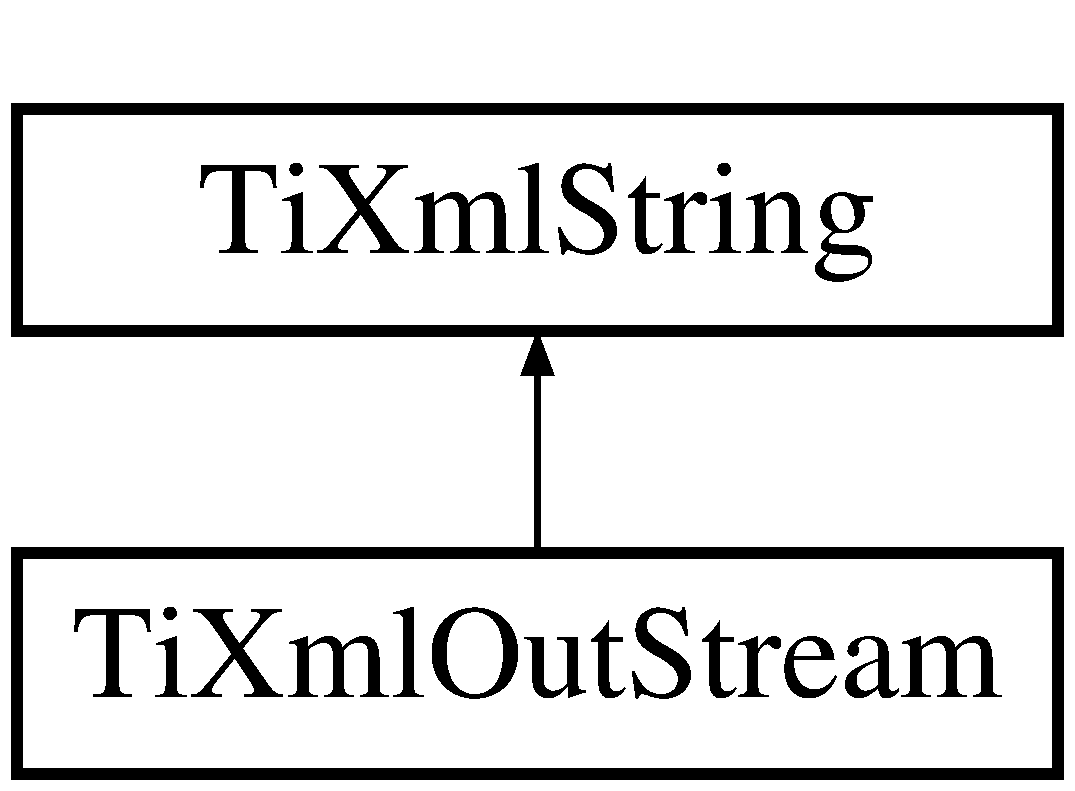
\includegraphics[height=2cm]{classTiXmlOutStream}
\end{center}
\end{figure}
\subsection*{Public Member Functions}
\begin{CompactItemize}
\item 
{\bf TiXmlOutStream} \& {\bf operator$<$$<$} (const {\bf TiXmlString} \&in)
\item 
{\bf TiXmlOutStream} \& {\bf operator$<$$<$} (const char $\ast$in)
\end{CompactItemize}


\subsection{Member Function Documentation}
\index{TiXmlOutStream@{TiXmlOutStream}!operator$<$$<$@{operator$<$$<$}}
\index{operator$<$$<$@{operator$<$$<$}!TiXmlOutStream@{TiXmlOutStream}}
\subsubsection[operator$<$$<$]{\setlength{\rightskip}{0pt plus 5cm}{\bf TiXmlOutStream}\& TiXmlOutStream::operator$<$$<$ (const {\bf TiXmlString} \& {\em in})\hspace{0.3cm}{\tt  [inline]}}\label{classTiXmlOutStream_3640dcb1c0903be3bc6966cdc9a79db6}


\index{TiXmlOutStream@{TiXmlOutStream}!operator$<$$<$@{operator$<$$<$}}
\index{operator$<$$<$@{operator$<$$<$}!TiXmlOutStream@{TiXmlOutStream}}
\subsubsection[operator$<$$<$]{\setlength{\rightskip}{0pt plus 5cm}{\bf TiXmlOutStream}\& TiXmlOutStream::operator$<$$<$ (const char $\ast$ {\em in})\hspace{0.3cm}{\tt  [inline]}}\label{classTiXmlOutStream_f2117e5a8cbfcb69544804ad2859bfb6}




The documentation for this class was generated from the following file:\begin{CompactItemize}
\item 
{\bf tinystr.h}\end{CompactItemize}

\section{TiXmlParsingData Class Reference}
\label{classTiXmlParsingData}\index{TiXmlParsingData@{TiXmlParsingData}}
\subsection*{Public Member Functions}
\begin{CompactItemize}
\item 
void {\bf Stamp} (const char $\ast$now, {\bf TiXmlEncoding} encoding)
\item 
const {\bf TiXmlCursor} \& {\bf Cursor} ()
\end{CompactItemize}
\subsection*{Friends}
\begin{CompactItemize}
\item 
class {\bf TiXmlDocument}
\end{CompactItemize}


\subsection{Member Function Documentation}
\index{TiXmlParsingData@{TiXmlParsingData}!Stamp@{Stamp}}
\index{Stamp@{Stamp}!TiXmlParsingData@{TiXmlParsingData}}
\subsubsection[Stamp]{\setlength{\rightskip}{0pt plus 5cm}void TiXmlParsingData::Stamp (const char $\ast$ {\em now}, \/  {\bf TiXmlEncoding} {\em encoding})}\label{classTiXmlParsingData_65cee8ab77a36c605db08c84b4c30a7d}




References TiXmlCursor::col, TiXmlCursor::row, TIXML\_\-ENCODING\_\-UTF8, TIXML\_\-UTF\_\-LEAD\_\-0, TIXML\_\-UTF\_\-LEAD\_\-1, TIXML\_\-UTF\_\-LEAD\_\-2, and TiXmlBase::utf8ByteTable.

Referenced by TiXmlDeclaration::Parse(), TiXmlText::Parse(), TiXmlAttribute::Parse(), TiXmlComment::Parse(), TiXmlUnknown::Parse(), TiXmlElement::Parse(), and TiXmlDocument::SetError().\index{TiXmlParsingData@{TiXmlParsingData}!Cursor@{Cursor}}
\index{Cursor@{Cursor}!TiXmlParsingData@{TiXmlParsingData}}
\subsubsection[Cursor]{\setlength{\rightskip}{0pt plus 5cm}const {\bf TiXmlCursor}\& TiXmlParsingData::Cursor ()\hspace{0.3cm}{\tt  [inline]}}\label{classTiXmlParsingData_56908a17d7d7a6b2e511e62cf1d40d05}




Referenced by TiXmlDeclaration::Parse(), TiXmlText::Parse(), TiXmlAttribute::Parse(), TiXmlComment::Parse(), TiXmlUnknown::Parse(), TiXmlElement::Parse(), TiXmlDocument::Parse(), and TiXmlDocument::SetError().

\subsection{Friends And Related Function Documentation}
\index{TiXmlParsingData@{TiXmlParsingData}!TiXmlDocument@{TiXmlDocument}}
\index{TiXmlDocument@{TiXmlDocument}!TiXmlParsingData@{TiXmlParsingData}}
\subsubsection[TiXmlDocument]{\setlength{\rightskip}{0pt plus 5cm}friend class {\bf TiXmlDocument}\hspace{0.3cm}{\tt  [friend]}}\label{classTiXmlParsingData_173617f6dfe902cf484ce5552b950475}




The documentation for this class was generated from the following file:\begin{CompactItemize}
\item 
{\bf tinyxmlparser.cpp}\end{CompactItemize}

\section{TiXmlPrinter Class Reference}
\label{classTiXmlPrinter}\index{TiXmlPrinter@{TiXmlPrinter}}
{\tt \#include $<$tinyxml.h$>$}

Inheritance diagram for TiXmlPrinter::\begin{figure}[H]
\begin{center}
\leavevmode
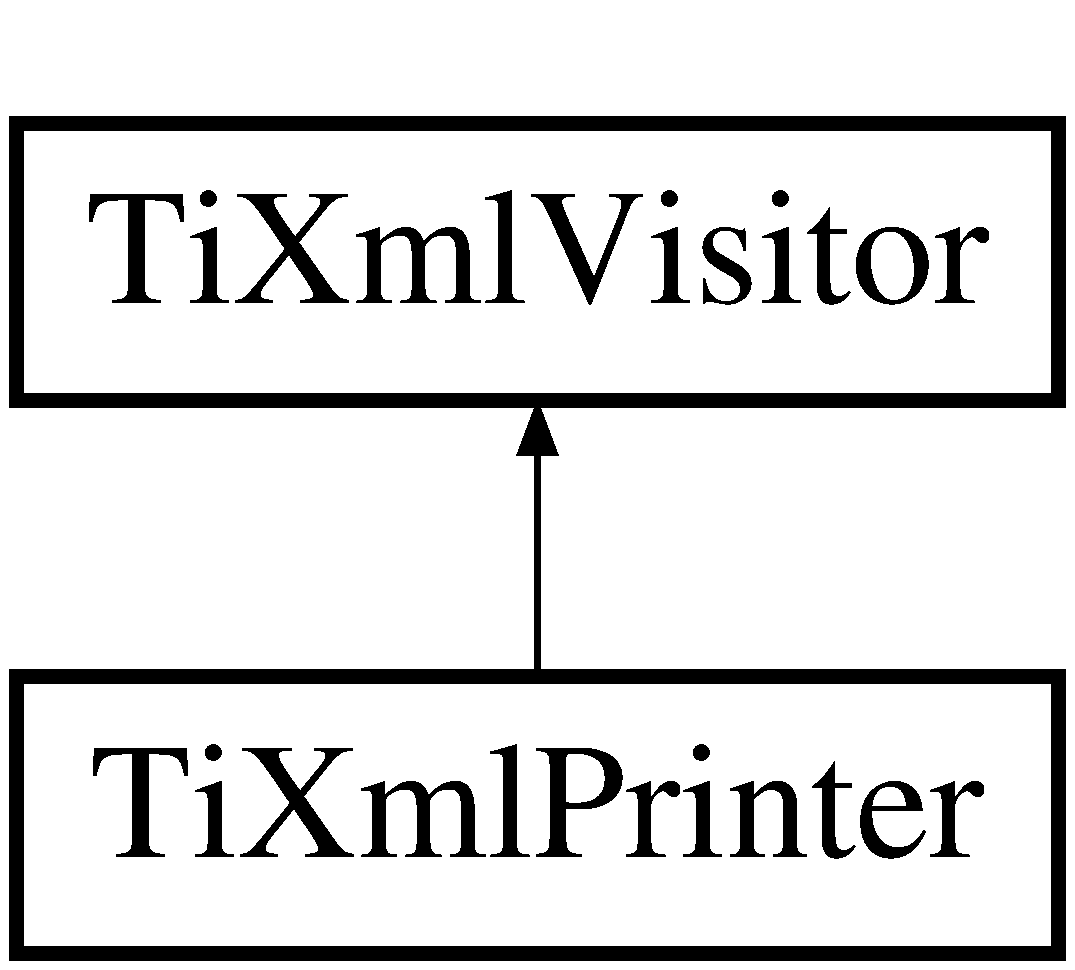
\includegraphics[height=2cm]{classTiXmlPrinter}
\end{center}
\end{figure}


\subsection{Detailed Description}
Print to memory functionality. The \doxyref{TiXmlPrinter}{p.}{classTiXmlPrinter} is useful when you need to:

\begin{enumerate}
\item Print to memory (especially in non-STL mode)\item Control formatting (line endings, etc.)\end{enumerate}


When constructed, the \doxyref{TiXmlPrinter}{p.}{classTiXmlPrinter} is in its default \char`\"{}pretty printing\char`\"{} mode. Before calling Accept() you can call methods to control the printing of the XML document. After \doxyref{TiXmlNode::Accept()}{p.}{classTiXmlNode_cc0f88b7462c6cb73809d410a4f5bb86} is called, the printed document can be accessed via the \doxyref{CStr()}{p.}{classTiXmlPrinter_859eede9597d3e0355b77757be48735e}, Str(), and \doxyref{Size()}{p.}{classTiXmlPrinter_d01375ae9199bd2f48252eaddce3039d} methods.

\doxyref{TiXmlPrinter}{p.}{classTiXmlPrinter} uses the Visitor API. 

\footnotesize\begin{verbatim}
	TiXmlPrinter printer;
	printer.SetIndent( "\t" );

	doc.Accept( &printer );
	fprintf( stdout, "%s", printer.CStr() );
	\end{verbatim}
\normalsize
 \subsection*{Public Member Functions}
\begin{CompactItemize}
\item 
{\bf TiXmlPrinter} ()
\item 
virtual bool {\bf VisitEnter} (const {\bf TiXmlDocument} \&doc)
\begin{CompactList}\small\item\em Visit a document. \item\end{CompactList}\item 
virtual bool {\bf VisitExit} (const {\bf TiXmlDocument} \&doc)
\begin{CompactList}\small\item\em Visit a document. \item\end{CompactList}\item 
virtual bool {\bf VisitEnter} (const {\bf TiXmlElement} \&element, const {\bf TiXmlAttribute} $\ast$firstAttribute)
\begin{CompactList}\small\item\em Visit an element. \item\end{CompactList}\item 
virtual bool {\bf VisitExit} (const {\bf TiXmlElement} \&element)
\begin{CompactList}\small\item\em Visit an element. \item\end{CompactList}\item 
virtual bool {\bf Visit} (const {\bf TiXmlDeclaration} \&declaration)
\begin{CompactList}\small\item\em Visit a declaration. \item\end{CompactList}\item 
virtual bool {\bf Visit} (const {\bf TiXmlText} \&text)
\begin{CompactList}\small\item\em Visit a text node. \item\end{CompactList}\item 
virtual bool {\bf Visit} (const {\bf TiXmlComment} \&comment)
\begin{CompactList}\small\item\em Visit a comment node. \item\end{CompactList}\item 
virtual bool {\bf Visit} (const {\bf TiXmlUnknown} \&unknown)
\begin{CompactList}\small\item\em Visit an unknow node. \item\end{CompactList}\item 
void {\bf SetIndent} (const char $\ast$\_\-indent)
\item 
const char $\ast$ {\bf Indent} ()
\begin{CompactList}\small\item\em Query the indention string. \item\end{CompactList}\item 
void {\bf SetLineBreak} (const char $\ast$\_\-lineBreak)
\item 
const char $\ast$ {\bf LineBreak} ()
\begin{CompactList}\small\item\em Query the current line breaking string. \item\end{CompactList}\item 
void {\bf SetStreamPrinting} ()
\item 
const char $\ast$ {\bf CStr} ()
\begin{CompactList}\small\item\em Return the result. \item\end{CompactList}\item 
size\_\-t {\bf Size} ()
\begin{CompactList}\small\item\em Return the length of the result string. \item\end{CompactList}\end{CompactItemize}


\subsection{Constructor \& Destructor Documentation}
\index{TiXmlPrinter@{TiXmlPrinter}!TiXmlPrinter@{TiXmlPrinter}}
\index{TiXmlPrinter@{TiXmlPrinter}!TiXmlPrinter@{TiXmlPrinter}}
\subsubsection[TiXmlPrinter]{\setlength{\rightskip}{0pt plus 5cm}TiXmlPrinter::TiXmlPrinter ()\hspace{0.3cm}{\tt  [inline]}}\label{classTiXmlPrinter_6539b864026c8667cd0bd5fdf4b41f43}




\subsection{Member Function Documentation}
\index{TiXmlPrinter@{TiXmlPrinter}!VisitEnter@{VisitEnter}}
\index{VisitEnter@{VisitEnter}!TiXmlPrinter@{TiXmlPrinter}}
\subsubsection[VisitEnter]{\setlength{\rightskip}{0pt plus 5cm}bool TiXmlPrinter::VisitEnter (const {\bf TiXmlDocument} \&)\hspace{0.3cm}{\tt  [virtual]}}\label{classTiXmlPrinter_2ec73087db26ff4d2c4316c56f861db7}


Visit a document. 



Reimplemented from {\bf TiXmlVisitor} \doxyref{}{p.}{classTiXmlVisitor_07baecb52dd7d8716ae2a48ad0956ee0}.\index{TiXmlPrinter@{TiXmlPrinter}!VisitExit@{VisitExit}}
\index{VisitExit@{VisitExit}!TiXmlPrinter@{TiXmlPrinter}}
\subsubsection[VisitExit]{\setlength{\rightskip}{0pt plus 5cm}bool TiXmlPrinter::VisitExit (const {\bf TiXmlDocument} \&)\hspace{0.3cm}{\tt  [virtual]}}\label{classTiXmlPrinter_0a636046fa589b6d7f3e5bd025b3f33e}


Visit a document. 



Reimplemented from {\bf TiXmlVisitor} \doxyref{}{p.}{classTiXmlVisitor_a0ade4f27087447e93974e975c3246ad}.\index{TiXmlPrinter@{TiXmlPrinter}!VisitEnter@{VisitEnter}}
\index{VisitEnter@{VisitEnter}!TiXmlPrinter@{TiXmlPrinter}}
\subsubsection[VisitEnter]{\setlength{\rightskip}{0pt plus 5cm}bool TiXmlPrinter::VisitEnter (const {\bf TiXmlElement} \&, \/  const {\bf TiXmlAttribute} $\ast$)\hspace{0.3cm}{\tt  [virtual]}}\label{classTiXmlPrinter_6dccaf5ee4979f13877690afe28721e8}


Visit an element. 



Reimplemented from {\bf TiXmlVisitor} \doxyref{}{p.}{classTiXmlVisitor_f6c6178ffa517bbdba95d70490875fff}.

References TiXmlText::CDATA(), TiXmlNode::FirstChild(), TiXmlNode::LastChild(), TiXmlAttribute::Next(), TiXmlAttribute::Print(), TiXmlNode::ToText(), and TiXmlNode::Value().\index{TiXmlPrinter@{TiXmlPrinter}!VisitExit@{VisitExit}}
\index{VisitExit@{VisitExit}!TiXmlPrinter@{TiXmlPrinter}}
\subsubsection[VisitExit]{\setlength{\rightskip}{0pt plus 5cm}bool TiXmlPrinter::VisitExit (const {\bf TiXmlElement} \&)\hspace{0.3cm}{\tt  [virtual]}}\label{classTiXmlPrinter_e6a1df8271df4bf62d7873c38e34aa69}


Visit an element. 



Reimplemented from {\bf TiXmlVisitor} \doxyref{}{p.}{classTiXmlVisitor_ec2b1f8116226d52f3a1b95dafd3a32c}.

References TiXmlNode::FirstChild(), and TiXmlNode::Value().\index{TiXmlPrinter@{TiXmlPrinter}!Visit@{Visit}}
\index{Visit@{Visit}!TiXmlPrinter@{TiXmlPrinter}}
\subsubsection[Visit]{\setlength{\rightskip}{0pt plus 5cm}bool TiXmlPrinter::Visit (const {\bf TiXmlDeclaration} \&)\hspace{0.3cm}{\tt  [virtual]}}\label{classTiXmlPrinter_daf7eec4dc43ad071ff52b60361574f5}


Visit a declaration. 



Reimplemented from {\bf TiXmlVisitor} \doxyref{}{p.}{classTiXmlVisitor_fad71c71ce6473fb9b4b64cd92de4a19}.

References TiXmlDeclaration::Print().\index{TiXmlPrinter@{TiXmlPrinter}!Visit@{Visit}}
\index{Visit@{Visit}!TiXmlPrinter@{TiXmlPrinter}}
\subsubsection[Visit]{\setlength{\rightskip}{0pt plus 5cm}bool TiXmlPrinter::Visit (const {\bf TiXmlText} \&)\hspace{0.3cm}{\tt  [virtual]}}\label{classTiXmlPrinter_0857c5d32c59b9a257f9a49cb9411df5}


Visit a text node. 



Reimplemented from {\bf TiXmlVisitor} \doxyref{}{p.}{classTiXmlVisitor_399b8ebca5cd14664974a32d2ce029e5}.

References TiXmlText::CDATA(), TiXmlBase::EncodeString(), TIXML\_\-STRING, TiXmlNode::Value(), and TiXmlNode::ValueTStr().\index{TiXmlPrinter@{TiXmlPrinter}!Visit@{Visit}}
\index{Visit@{Visit}!TiXmlPrinter@{TiXmlPrinter}}
\subsubsection[Visit]{\setlength{\rightskip}{0pt plus 5cm}bool TiXmlPrinter::Visit (const {\bf TiXmlComment} \&)\hspace{0.3cm}{\tt  [virtual]}}\label{classTiXmlPrinter_9870423f5603630e6142f6bdb66dfb57}


Visit a comment node. 



Reimplemented from {\bf TiXmlVisitor} \doxyref{}{p.}{classTiXmlVisitor_53a60e7a528627b31af3161972cc7fa2}.

References TiXmlNode::Value().\index{TiXmlPrinter@{TiXmlPrinter}!Visit@{Visit}}
\index{Visit@{Visit}!TiXmlPrinter@{TiXmlPrinter}}
\subsubsection[Visit]{\setlength{\rightskip}{0pt plus 5cm}bool TiXmlPrinter::Visit (const {\bf TiXmlUnknown} \&)\hspace{0.3cm}{\tt  [virtual]}}\label{classTiXmlPrinter_08591a15c9a07afa83c24e08b03d6358}


Visit an unknow node. 



Reimplemented from {\bf TiXmlVisitor} \doxyref{}{p.}{classTiXmlVisitor_7e284d607d275c51dac1adb58159ce28}.

References TiXmlNode::Value().\index{TiXmlPrinter@{TiXmlPrinter}!SetIndent@{SetIndent}}
\index{SetIndent@{SetIndent}!TiXmlPrinter@{TiXmlPrinter}}
\subsubsection[SetIndent]{\setlength{\rightskip}{0pt plus 5cm}void TiXmlPrinter::SetIndent (const char $\ast$ {\em \_\-indent})\hspace{0.3cm}{\tt  [inline]}}\label{classTiXmlPrinter_213377a4070c7e625bae59716b089e5e}


Set the indent characters for printing. By default 4 spaces but tab ($\backslash$t) is also useful, or null/empty string for no indentation. \index{TiXmlPrinter@{TiXmlPrinter}!Indent@{Indent}}
\index{Indent@{Indent}!TiXmlPrinter@{TiXmlPrinter}}
\subsubsection[Indent]{\setlength{\rightskip}{0pt plus 5cm}const char$\ast$ TiXmlPrinter::Indent ()\hspace{0.3cm}{\tt  [inline]}}\label{classTiXmlPrinter_bb33ec7d4bad6aaeb57f4304394b133d}


Query the indention string. 

\index{TiXmlPrinter@{TiXmlPrinter}!SetLineBreak@{SetLineBreak}}
\index{SetLineBreak@{SetLineBreak}!TiXmlPrinter@{TiXmlPrinter}}
\subsubsection[SetLineBreak]{\setlength{\rightskip}{0pt plus 5cm}void TiXmlPrinter::SetLineBreak (const char $\ast$ {\em \_\-lineBreak})\hspace{0.3cm}{\tt  [inline]}}\label{classTiXmlPrinter_4be1e37e69e3858c59635aa947174fe6}


Set the line breaking string. By default set to newline (\par
). Some operating systems prefer other characters, or can be set to the null/empty string for no indenation. \index{TiXmlPrinter@{TiXmlPrinter}!LineBreak@{LineBreak}}
\index{LineBreak@{LineBreak}!TiXmlPrinter@{TiXmlPrinter}}
\subsubsection[LineBreak]{\setlength{\rightskip}{0pt plus 5cm}const char$\ast$ TiXmlPrinter::LineBreak ()\hspace{0.3cm}{\tt  [inline]}}\label{classTiXmlPrinter_11f1b4804a460b175ec244eb5724d96d}


Query the current line breaking string. 

\index{TiXmlPrinter@{TiXmlPrinter}!SetStreamPrinting@{SetStreamPrinting}}
\index{SetStreamPrinting@{SetStreamPrinting}!TiXmlPrinter@{TiXmlPrinter}}
\subsubsection[SetStreamPrinting]{\setlength{\rightskip}{0pt plus 5cm}void TiXmlPrinter::SetStreamPrinting ()\hspace{0.3cm}{\tt  [inline]}}\label{classTiXmlPrinter_b23a90629e374cb1cadca090468bbd19}


Switch over to \char`\"{}stream printing\char`\"{} which is the most dense formatting without linebreaks. Common when the XML is needed for network transmission. \index{TiXmlPrinter@{TiXmlPrinter}!CStr@{CStr}}
\index{CStr@{CStr}!TiXmlPrinter@{TiXmlPrinter}}
\subsubsection[CStr]{\setlength{\rightskip}{0pt plus 5cm}const char$\ast$ TiXmlPrinter::CStr ()\hspace{0.3cm}{\tt  [inline]}}\label{classTiXmlPrinter_859eede9597d3e0355b77757be48735e}


Return the result. 

\index{TiXmlPrinter@{TiXmlPrinter}!Size@{Size}}
\index{Size@{Size}!TiXmlPrinter@{TiXmlPrinter}}
\subsubsection[Size]{\setlength{\rightskip}{0pt plus 5cm}size\_\-t TiXmlPrinter::Size ()\hspace{0.3cm}{\tt  [inline]}}\label{classTiXmlPrinter_d01375ae9199bd2f48252eaddce3039d}


Return the length of the result string. 



The documentation for this class was generated from the following files:\begin{CompactItemize}
\item 
{\bf tinyxml.h}\item 
{\bf tinyxml.cpp}\end{CompactItemize}

\section{TiXmlString Class Reference}
\label{classTiXmlString}\index{TiXmlString@{TiXmlString}}
{\tt \#include $<$tinystr.h$>$}

Inheritance diagram for TiXmlString::\begin{figure}[H]
\begin{center}
\leavevmode
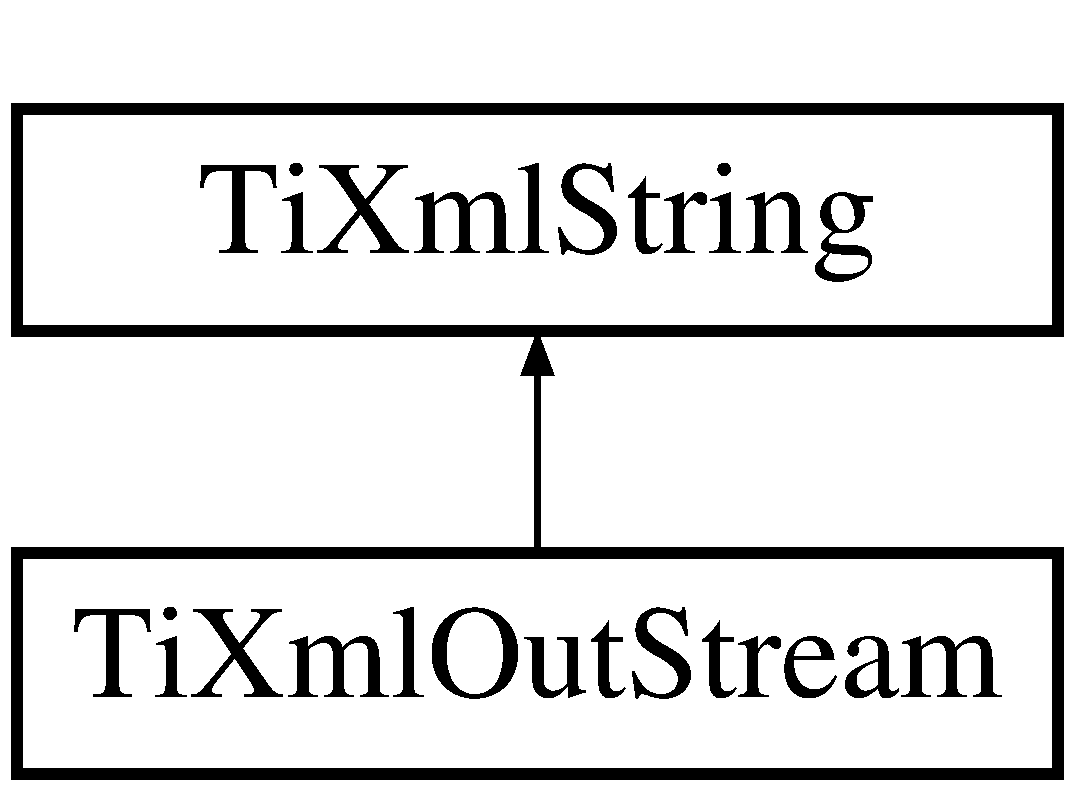
\includegraphics[height=2cm]{classTiXmlString}
\end{center}
\end{figure}
\subsection*{Public Types}
\begin{CompactItemize}
\item 
typedef size\_\-t {\bf size\_\-type}
\end{CompactItemize}
\subsection*{Public Member Functions}
\begin{CompactItemize}
\item 
{\bf TiXmlString} ()
\item 
{\bf TiXmlString} (const {\bf TiXmlString} \&copy)
\item 
TIXML\_\-EXPLICIT {\bf TiXmlString} (const char $\ast$copy)
\item 
TIXML\_\-EXPLICIT {\bf TiXmlString} (const char $\ast$str, {\bf size\_\-type} len)
\item 
{\bf $\sim$TiXmlString} ()
\item 
{\bf TiXmlString} \& {\bf operator=} (const char $\ast$copy)
\item 
{\bf TiXmlString} \& {\bf operator=} (const {\bf TiXmlString} \&copy)
\item 
{\bf TiXmlString} \& {\bf operator+=} (const char $\ast$suffix)
\item 
{\bf TiXmlString} \& {\bf operator+=} (char single)
\item 
{\bf TiXmlString} \& {\bf operator+=} (const {\bf TiXmlString} \&suffix)
\item 
const char $\ast$ {\bf c\_\-str} () const 
\item 
const char $\ast$ {\bf data} () const 
\item 
{\bf size\_\-type} {\bf length} () const 
\item 
{\bf size\_\-type} {\bf size} () const 
\item 
bool {\bf empty} () const 
\item 
{\bf size\_\-type} {\bf capacity} () const 
\item 
const char \& {\bf at} ({\bf size\_\-type} index) const 
\item 
char \& {\bf operator[$\,$]} ({\bf size\_\-type} index) const 
\item 
{\bf size\_\-type} {\bf find} (char lookup) const 
\item 
{\bf size\_\-type} {\bf find} (char tofind, {\bf size\_\-type} offset) const 
\item 
void {\bf clear} ()
\item 
void {\bf reserve} ({\bf size\_\-type} cap)
\item 
{\bf TiXmlString} \& {\bf assign} (const char $\ast$str, {\bf size\_\-type} len)
\item 
{\bf TiXmlString} \& {\bf append} (const char $\ast$str, {\bf size\_\-type} len)
\item 
void {\bf swap} ({\bf TiXmlString} \&other)
\end{CompactItemize}
\subsection*{Static Public Attributes}
\begin{CompactItemize}
\item 
static const {\bf size\_\-type} {\bf npos} = static\_\-cast$<$ {\bf TiXmlString::size\_\-type} $>$(-1)
\end{CompactItemize}
\subsection*{Classes}
\begin{CompactItemize}
\item 
struct \textbf{Rep}
\end{CompactItemize}


\subsection{Member Typedef Documentation}
\index{TiXmlString@{TiXmlString}!size\_\-type@{size\_\-type}}
\index{size\_\-type@{size\_\-type}!TiXmlString@{TiXmlString}}
\subsubsection[size\_\-type]{\setlength{\rightskip}{0pt plus 5cm}typedef size\_\-t {\bf TiXmlString::size\_\-type}}\label{classTiXmlString_beb2c1893a04c17904f7c06546d0b971}




\subsection{Constructor \& Destructor Documentation}
\index{TiXmlString@{TiXmlString}!TiXmlString@{TiXmlString}}
\index{TiXmlString@{TiXmlString}!TiXmlString@{TiXmlString}}
\subsubsection[TiXmlString]{\setlength{\rightskip}{0pt plus 5cm}TiXmlString::TiXmlString ()\hspace{0.3cm}{\tt  [inline]}}\label{classTiXmlString_342f61e0fc2244df300b73aedf6d3fef}


\index{TiXmlString@{TiXmlString}!TiXmlString@{TiXmlString}}
\index{TiXmlString@{TiXmlString}!TiXmlString@{TiXmlString}}
\subsubsection[TiXmlString]{\setlength{\rightskip}{0pt plus 5cm}TiXmlString::TiXmlString (const {\bf TiXmlString} \& {\em copy})\hspace{0.3cm}{\tt  [inline]}}\label{classTiXmlString_c80fe17693a438c9ab2591664743fcb6}




References data(), and length().\index{TiXmlString@{TiXmlString}!TiXmlString@{TiXmlString}}
\index{TiXmlString@{TiXmlString}!TiXmlString@{TiXmlString}}
\subsubsection[TiXmlString]{\setlength{\rightskip}{0pt plus 5cm}TIXML\_\-EXPLICIT TiXmlString::TiXmlString (const char $\ast$ {\em copy})\hspace{0.3cm}{\tt  [inline]}}\label{classTiXmlString_a3b32bd2891a757c9f36c21db44c81d2}




References length().\index{TiXmlString@{TiXmlString}!TiXmlString@{TiXmlString}}
\index{TiXmlString@{TiXmlString}!TiXmlString@{TiXmlString}}
\subsubsection[TiXmlString]{\setlength{\rightskip}{0pt plus 5cm}TIXML\_\-EXPLICIT TiXmlString::TiXmlString (const char $\ast$ {\em str}, \/  {\bf size\_\-type} {\em len})\hspace{0.3cm}{\tt  [inline]}}\label{classTiXmlString_4b17ea5c5db986f14827223dfa8f1547}


\index{TiXmlString@{TiXmlString}!$\sim$TiXmlString@{$\sim$TiXmlString}}
\index{$\sim$TiXmlString@{$\sim$TiXmlString}!TiXmlString@{TiXmlString}}
\subsubsection[$\sim$TiXmlString]{\setlength{\rightskip}{0pt plus 5cm}TiXmlString::$\sim$TiXmlString ()\hspace{0.3cm}{\tt  [inline]}}\label{classTiXmlString_7ac03f581ca3422c4808162ab14f3450}




\subsection{Member Function Documentation}
\index{TiXmlString@{TiXmlString}!operator=@{operator=}}
\index{operator=@{operator=}!TiXmlString@{TiXmlString}}
\subsubsection[operator=]{\setlength{\rightskip}{0pt plus 5cm}{\bf TiXmlString}\& TiXmlString::operator= (const char $\ast$ {\em copy})\hspace{0.3cm}{\tt  [inline]}}\label{classTiXmlString_e0bc6147afc0ec2aa0da3a3c0a8fcfb0}




References assign().\index{TiXmlString@{TiXmlString}!operator=@{operator=}}
\index{operator=@{operator=}!TiXmlString@{TiXmlString}}
\subsubsection[operator=]{\setlength{\rightskip}{0pt plus 5cm}{\bf TiXmlString}\& TiXmlString::operator= (const {\bf TiXmlString} \& {\em copy})\hspace{0.3cm}{\tt  [inline]}}\label{classTiXmlString_b1f1f5d3eceaa0f22d0a7e6055ea81b0}




References assign(), length(), and start().\index{TiXmlString@{TiXmlString}!operator+=@{operator+=}}
\index{operator+=@{operator+=}!TiXmlString@{TiXmlString}}
\subsubsection[operator+=]{\setlength{\rightskip}{0pt plus 5cm}{\bf TiXmlString}\& TiXmlString::operator+= (const char $\ast$ {\em suffix})\hspace{0.3cm}{\tt  [inline]}}\label{classTiXmlString_b56336ac2aa2a08d24a71eb9a2b502a5}




References append().\index{TiXmlString@{TiXmlString}!operator+=@{operator+=}}
\index{operator+=@{operator+=}!TiXmlString@{TiXmlString}}
\subsubsection[operator+=]{\setlength{\rightskip}{0pt plus 5cm}{\bf TiXmlString}\& TiXmlString::operator+= (char {\em single})\hspace{0.3cm}{\tt  [inline]}}\label{classTiXmlString_6aa09d5240470b76d54ec709e04f8c13}




References append().\index{TiXmlString@{TiXmlString}!operator+=@{operator+=}}
\index{operator+=@{operator+=}!TiXmlString@{TiXmlString}}
\subsubsection[operator+=]{\setlength{\rightskip}{0pt plus 5cm}{\bf TiXmlString}\& TiXmlString::operator+= (const {\bf TiXmlString} \& {\em suffix})\hspace{0.3cm}{\tt  [inline]}}\label{classTiXmlString_fdcae5ea2b4d9e194dc21226b817f417}




References append(), data(), and length().\index{TiXmlString@{TiXmlString}!c\_\-str@{c\_\-str}}
\index{c\_\-str@{c\_\-str}!TiXmlString@{TiXmlString}}
\subsubsection[c\_\-str]{\setlength{\rightskip}{0pt plus 5cm}const char$\ast$ TiXmlString::c\_\-str () const\hspace{0.3cm}{\tt  [inline]}}\label{classTiXmlString_5581ca641d915551d3cda90f8e7bf49b}




Referenced by find(), operator$<$(), and operator==().\index{TiXmlString@{TiXmlString}!data@{data}}
\index{data@{data}!TiXmlString@{TiXmlString}}
\subsubsection[data]{\setlength{\rightskip}{0pt plus 5cm}const char$\ast$ TiXmlString::data () const\hspace{0.3cm}{\tt  [inline]}}\label{classTiXmlString_00abc60f135c7ca1951c7334cc2c7993}




Referenced by operator+=(), reserve(), and TiXmlString().\index{TiXmlString@{TiXmlString}!length@{length}}
\index{length@{length}!TiXmlString@{TiXmlString}}
\subsubsection[length]{\setlength{\rightskip}{0pt plus 5cm}{\bf size\_\-type} TiXmlString::length () const\hspace{0.3cm}{\tt  [inline]}}\label{classTiXmlString_3202f27d139a3fac79205f1f3c707727}




Referenced by append(), at(), find(), operator+(), operator+=(), operator=(), operator==(), operator[$\,$](), reserve(), and TiXmlString().\index{TiXmlString@{TiXmlString}!size@{size}}
\index{size@{size}!TiXmlString@{TiXmlString}}
\subsubsection[size]{\setlength{\rightskip}{0pt plus 5cm}{\bf size\_\-type} TiXmlString::size () const\hspace{0.3cm}{\tt  [inline]}}\label{classTiXmlString_96103e5c0f67e987fa48527e1f47a1f6}


\index{TiXmlString@{TiXmlString}!empty@{empty}}
\index{empty@{empty}!TiXmlString@{TiXmlString}}
\subsubsection[empty]{\setlength{\rightskip}{0pt plus 5cm}bool TiXmlString::empty () const\hspace{0.3cm}{\tt  [inline]}}\label{classTiXmlString_9a61e1d11cdb71bea4a4ed79caa793f4}


\index{TiXmlString@{TiXmlString}!capacity@{capacity}}
\index{capacity@{capacity}!TiXmlString@{TiXmlString}}
\subsubsection[capacity]{\setlength{\rightskip}{0pt plus 5cm}{\bf size\_\-type} TiXmlString::capacity () const\hspace{0.3cm}{\tt  [inline]}}\label{classTiXmlString_76e4d6aba7845f4cf9c02332a5fbf916}




Referenced by append(), assign(), and reserve().\index{TiXmlString@{TiXmlString}!at@{at}}
\index{at@{at}!TiXmlString@{TiXmlString}}
\subsubsection[at]{\setlength{\rightskip}{0pt plus 5cm}const char\& TiXmlString::at ({\bf size\_\-type} {\em index}) const\hspace{0.3cm}{\tt  [inline]}}\label{classTiXmlString_6763093267bbdecbf03f8840bc349877}




References length().\index{TiXmlString@{TiXmlString}!operator[]@{operator[]}}
\index{operator[]@{operator[]}!TiXmlString@{TiXmlString}}
\subsubsection[operator[]]{\setlength{\rightskip}{0pt plus 5cm}char\& TiXmlString::operator[$\,$] ({\bf size\_\-type} {\em index}) const\hspace{0.3cm}{\tt  [inline]}}\label{classTiXmlString_e8cdc1d46c538536b786f7ae03c0c1d9}




References length().\index{TiXmlString@{TiXmlString}!find@{find}}
\index{find@{find}!TiXmlString@{TiXmlString}}
\subsubsection[find]{\setlength{\rightskip}{0pt plus 5cm}{\bf size\_\-type} TiXmlString::find (char {\em lookup}) const\hspace{0.3cm}{\tt  [inline]}}\label{classTiXmlString_5c2b368b5eafe075fd9565cbcbd4c2f9}


\index{TiXmlString@{TiXmlString}!find@{find}}
\index{find@{find}!TiXmlString@{TiXmlString}}
\subsubsection[find]{\setlength{\rightskip}{0pt plus 5cm}{\bf size\_\-type} TiXmlString::find (char {\em tofind}, \/  {\bf size\_\-type} {\em offset}) const\hspace{0.3cm}{\tt  [inline]}}\label{classTiXmlString_5f2a6fd565751410b392f249a9786db4}




References c\_\-str(), length(), and npos.\index{TiXmlString@{TiXmlString}!clear@{clear}}
\index{clear@{clear}!TiXmlString@{TiXmlString}}
\subsubsection[clear]{\setlength{\rightskip}{0pt plus 5cm}void TiXmlString::clear ()\hspace{0.3cm}{\tt  [inline]}}\label{classTiXmlString_b20e06e4c666abf3bdbfb3a1191d4888}


\index{TiXmlString@{TiXmlString}!reserve@{reserve}}
\index{reserve@{reserve}!TiXmlString@{TiXmlString}}
\subsubsection[reserve]{\setlength{\rightskip}{0pt plus 5cm}void TiXmlString::reserve ({\bf size\_\-type} {\em cap})}\label{classTiXmlString_88ecf9f0f00cb5c67b6b637958d7049c}




References capacity(), data(), init(), length(), start(), and swap().

Referenced by append(), and operator+().\index{TiXmlString@{TiXmlString}!assign@{assign}}
\index{assign@{assign}!TiXmlString@{TiXmlString}}
\subsubsection[assign]{\setlength{\rightskip}{0pt plus 5cm}{\bf TiXmlString} \& TiXmlString::assign (const char $\ast$ {\em str}, \/  {\bf size\_\-type} {\em len})}\label{classTiXmlString_c72f3d9149b7812c1e6c59402014d0d5}




References capacity(), init(), start(), and swap().

Referenced by operator=().\index{TiXmlString@{TiXmlString}!append@{append}}
\index{append@{append}!TiXmlString@{TiXmlString}}
\subsubsection[append]{\setlength{\rightskip}{0pt plus 5cm}{\bf TiXmlString} \& TiXmlString::append (const char $\ast$ {\em str}, \/  {\bf size\_\-type} {\em len})}\label{classTiXmlString_d44b21700d2ec24a511367b222b643fb}




References capacity(), length(), and reserve().

Referenced by operator+(), and operator+=().\index{TiXmlString@{TiXmlString}!swap@{swap}}
\index{swap@{swap}!TiXmlString@{TiXmlString}}
\subsubsection[swap]{\setlength{\rightskip}{0pt plus 5cm}void TiXmlString::swap ({\bf TiXmlString} \& {\em other})\hspace{0.3cm}{\tt  [inline]}}\label{classTiXmlString_a392cbc180752a79f007f4f9280c7762}




References rep\_\-.

Referenced by assign(), and reserve().

\subsection{Member Data Documentation}
\index{TiXmlString@{TiXmlString}!npos@{npos}}
\index{npos@{npos}!TiXmlString@{TiXmlString}}
\subsubsection[npos]{\setlength{\rightskip}{0pt plus 5cm}const {\bf TiXmlString::size\_\-type} {\bf TiXmlString::npos} = static\_\-cast$<$ {\bf TiXmlString::size\_\-type} $>$(-1)\hspace{0.3cm}{\tt  [static]}}\label{classTiXmlString_8f4422d227088dc7bec96f479b275d0a}




Referenced by find().

The documentation for this class was generated from the following files:\begin{CompactItemize}
\item 
{\bf tinystr.h}\item 
{\bf tinystr.cpp}\end{CompactItemize}

\section{TiXmlText Class Reference}
\label{classTiXmlText}\index{TiXmlText@{TiXmlText}}
{\tt \#include $<$tinyxml.h$>$}

Inheritance diagram for TiXmlText::\begin{figure}[H]
\begin{center}
\leavevmode
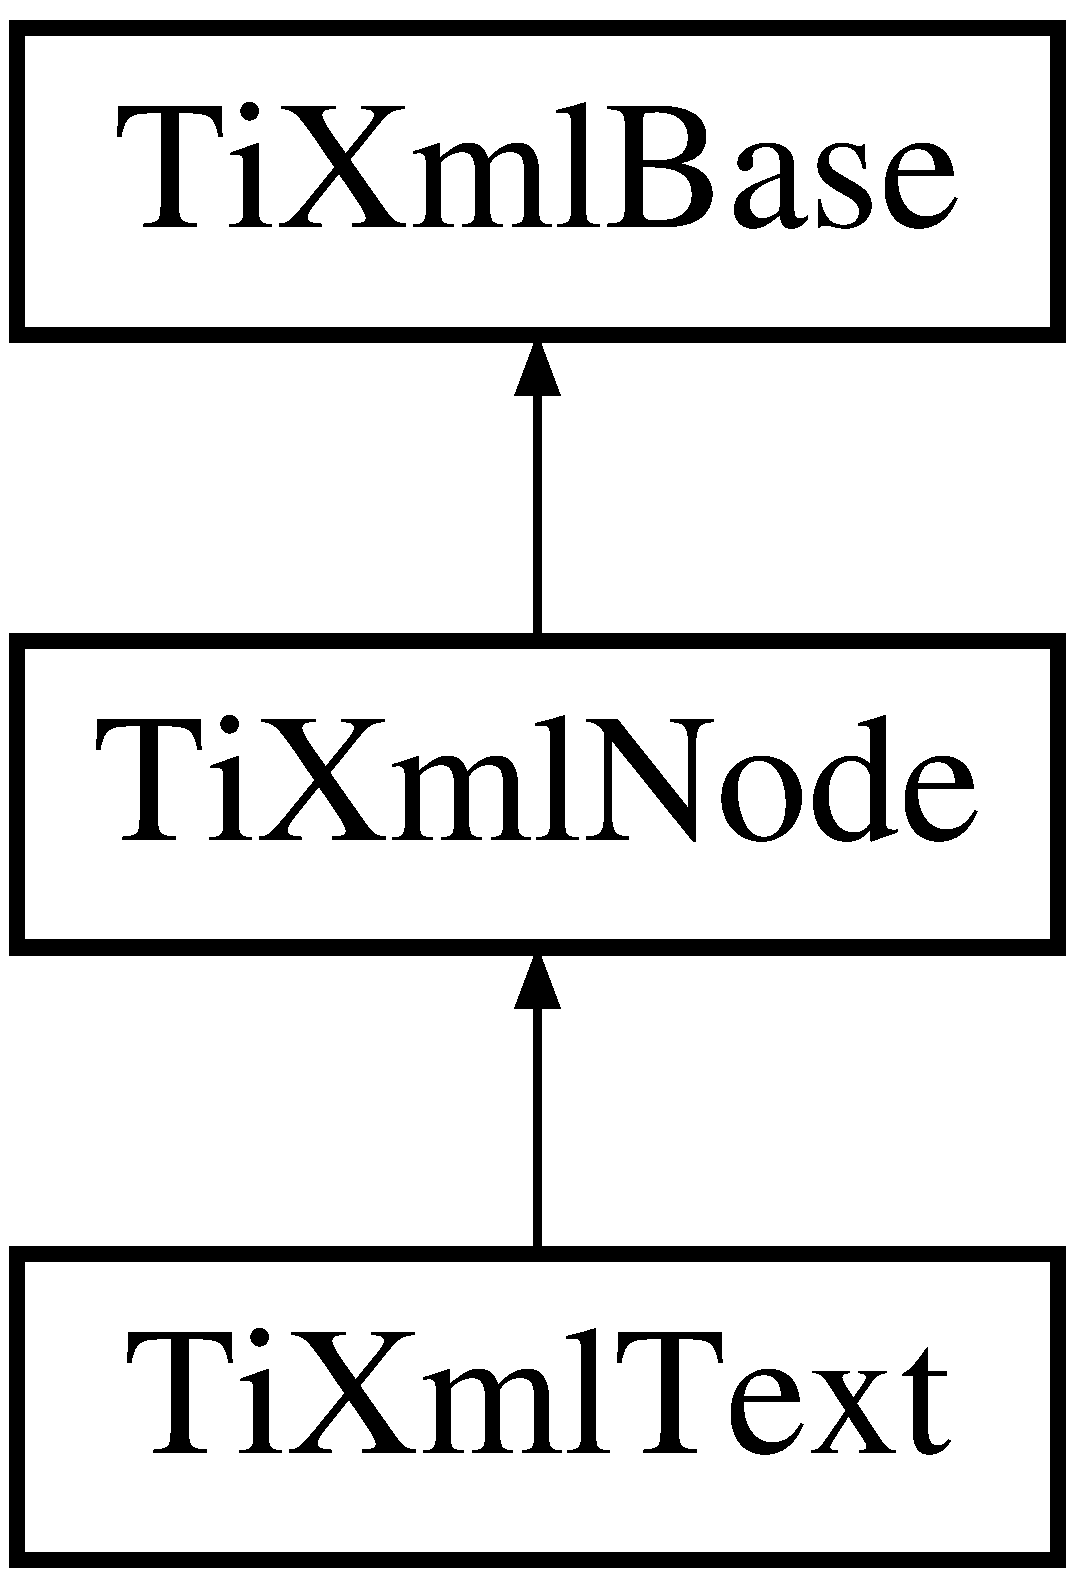
\includegraphics[height=3cm]{classTiXmlText}
\end{center}
\end{figure}


\subsection{Detailed Description}
XML text. A text node can have 2 ways to output the next. \char`\"{}normal\char`\"{} output and CDATA. It will default to the mode it was parsed from the XML file and you generally want to leave it alone, but you can change the output mode with \doxyref{SetCDATA()}{p.}{classTiXmlText_cb17ff7c5d09b2c839393445a3de5ea9} and query it with \doxyref{CDATA()}{p.}{classTiXmlText_d1a6a6b83fa2271022dd97c072a2b586}. \subsection*{Public Member Functions}
\begin{CompactItemize}
\item 
{\bf TiXmlText} (const char $\ast$initValue)
\item 
virtual {\bf $\sim$TiXmlText} ()
\item 
{\bf TiXmlText} (const {\bf TiXmlText} \&copy)
\item 
void {\bf operator=} (const {\bf TiXmlText} \&base)
\item 
virtual void {\bf Print} (FILE $\ast$cfile, int depth) const 
\item 
bool {\bf CDATA} () const 
\begin{CompactList}\small\item\em Queries whether this represents text using a CDATA section. \item\end{CompactList}\item 
void {\bf SetCDATA} (bool \_\-cdata)
\begin{CompactList}\small\item\em Turns on or off a CDATA representation of text. \item\end{CompactList}\item 
virtual const char $\ast$ {\bf Parse} (const char $\ast$p, {\bf TiXmlParsingData} $\ast$data, {\bf TiXmlEncoding} encoding)
\item 
virtual const {\bf TiXmlText} $\ast$ {\bf ToText} () const 
\begin{CompactList}\small\item\em Cast to a more defined type. Will return null not of the requested type. \item\end{CompactList}\item 
virtual {\bf TiXmlText} $\ast$ {\bf ToText} ()
\begin{CompactList}\small\item\em Cast to a more defined type. Will return null not of the requested type. \item\end{CompactList}\item 
virtual bool {\bf Accept} ({\bf TiXmlVisitor} $\ast$content) const 
\end{CompactItemize}
\subsection*{Protected Member Functions}
\begin{CompactItemize}
\item 
virtual {\bf TiXmlNode} $\ast$ {\bf Clone} () const 
\begin{CompactList}\small\item\em [internal use] Creates a new Element and returns it. \item\end{CompactList}\item 
void {\bf CopyTo} ({\bf TiXmlText} $\ast$target) const 
\item 
bool {\bf Blank} () const 
\end{CompactItemize}
\subsection*{Friends}
\begin{CompactItemize}
\item 
class {\bf TiXmlElement}
\end{CompactItemize}


\subsection{Constructor \& Destructor Documentation}
\index{TiXmlText@{TiXmlText}!TiXmlText@{TiXmlText}}
\index{TiXmlText@{TiXmlText}!TiXmlText@{TiXmlText}}
\subsubsection[TiXmlText]{\setlength{\rightskip}{0pt plus 5cm}TiXmlText::TiXmlText (const char $\ast$ {\em initValue})\hspace{0.3cm}{\tt  [inline]}}\label{classTiXmlText_f659e77c6b87d684827f35a8f4895960}


Constructor for text element. By default, it is treated as normal, encoded text. If you want it be output as a CDATA text element, set the parameter \_\-cdata to 'true' 

References TiXmlNode::SetValue().

Referenced by Clone().\index{TiXmlText@{TiXmlText}!$\sim$TiXmlText@{$\sim$TiXmlText}}
\index{$\sim$TiXmlText@{$\sim$TiXmlText}!TiXmlText@{TiXmlText}}
\subsubsection[$\sim$TiXmlText]{\setlength{\rightskip}{0pt plus 5cm}virtual TiXmlText::$\sim$TiXmlText ()\hspace{0.3cm}{\tt  [inline, virtual]}}\label{classTiXmlText_829a4bd2d8d2461c333eb4f3f5b1b3d2}


\index{TiXmlText@{TiXmlText}!TiXmlText@{TiXmlText}}
\index{TiXmlText@{TiXmlText}!TiXmlText@{TiXmlText}}
\subsubsection[TiXmlText]{\setlength{\rightskip}{0pt plus 5cm}TiXmlText::TiXmlText (const {\bf TiXmlText} \& {\em copy})\hspace{0.3cm}{\tt  [inline]}}\label{classTiXmlText_8d2cc1b4af2208cbb0171cf20f6815d1}




References CopyTo().

\subsection{Member Function Documentation}
\index{TiXmlText@{TiXmlText}!operator=@{operator=}}
\index{operator=@{operator=}!TiXmlText@{TiXmlText}}
\subsubsection[operator=]{\setlength{\rightskip}{0pt plus 5cm}void TiXmlText::operator= (const {\bf TiXmlText} \& {\em base})\hspace{0.3cm}{\tt  [inline]}}\label{classTiXmlText_f5f15d40d048cea7cab9d0eb4fd8a7d2}




References CopyTo().\index{TiXmlText@{TiXmlText}!Print@{Print}}
\index{Print@{Print}!TiXmlText@{TiXmlText}}
\subsubsection[Print]{\setlength{\rightskip}{0pt plus 5cm}void TiXmlText::Print (FILE $\ast$ {\em cfile}, \/  int {\em depth}) const\hspace{0.3cm}{\tt  [virtual]}}\label{classTiXmlText_e74d56c5b3ddec6cc3103dd51821af92}


All TinyXml classes can print themselves to a filestream or the string class (\doxyref{TiXmlString}{p.}{classTiXmlString} in non-STL mode, std::string in STL mode.) Either or both cfile and str can be null.

This is a formatted print, and will insert tabs and newlines.

(For an unformatted stream, use the $<$$<$ operator.) 

Implements {\bf TiXmlBase} \doxyref{}{p.}{classTiXmlBase_0de56b3f2ef14c65091a3b916437b512}.

References TiXmlBase::EncodeString(), TIXML\_\-STRING, and TiXmlNode::value.\index{TiXmlText@{TiXmlText}!CDATA@{CDATA}}
\index{CDATA@{CDATA}!TiXmlText@{TiXmlText}}
\subsubsection[CDATA]{\setlength{\rightskip}{0pt plus 5cm}bool TiXmlText::CDATA () const\hspace{0.3cm}{\tt  [inline]}}\label{classTiXmlText_d1a6a6b83fa2271022dd97c072a2b586}


Queries whether this represents text using a CDATA section. 



Referenced by TiXmlPrinter::Visit(), and TiXmlPrinter::VisitEnter().\index{TiXmlText@{TiXmlText}!SetCDATA@{SetCDATA}}
\index{SetCDATA@{SetCDATA}!TiXmlText@{TiXmlText}}
\subsubsection[SetCDATA]{\setlength{\rightskip}{0pt plus 5cm}void TiXmlText::SetCDATA (bool {\em \_\-cdata})\hspace{0.3cm}{\tt  [inline]}}\label{classTiXmlText_cb17ff7c5d09b2c839393445a3de5ea9}


Turns on or off a CDATA representation of text. 



Referenced by TiXmlNode::Identify().\index{TiXmlText@{TiXmlText}!Parse@{Parse}}
\index{Parse@{Parse}!TiXmlText@{TiXmlText}}
\subsubsection[Parse]{\setlength{\rightskip}{0pt plus 5cm}const char $\ast$ TiXmlText::Parse (const char $\ast$ {\em p}, \/  {\bf TiXmlParsingData} $\ast$ {\em data}, \/  {\bf TiXmlEncoding} {\em encoding})\hspace{0.3cm}{\tt  [virtual]}}\label{classTiXmlText_8d2dcfa41fc73d3e62dacc2fcf633819}




Implements {\bf TiXmlBase} \doxyref{}{p.}{classTiXmlBase_00e4edb0219d00a1379c856e5a1d2025}.

References TiXmlParsingData::Cursor(), TiXmlNode::GetDocument(), TiXmlBase::location, TiXmlBase::ReadText(), TiXmlDocument::SetError(), TiXmlParsingData::Stamp(), TiXmlBase::StringEqual(), TiXmlBase::TIXML\_\-ERROR\_\-PARSING\_\-CDATA, TIXML\_\-STRING, and TiXmlNode::value.

Referenced by TiXmlElement::ReadValue().\index{TiXmlText@{TiXmlText}!ToText@{ToText}}
\index{ToText@{ToText}!TiXmlText@{TiXmlText}}
\subsubsection[ToText]{\setlength{\rightskip}{0pt plus 5cm}virtual const {\bf TiXmlText}$\ast$ TiXmlText::ToText () const\hspace{0.3cm}{\tt  [inline, virtual]}}\label{classTiXmlText_895bf34ffad17f7439ab2a52b9651648}


Cast to a more defined type. Will return null not of the requested type. 



Reimplemented from {\bf TiXmlNode} \doxyref{}{p.}{classTiXmlNode_95a46a52c525992d6b4ee08beb14cd69}.\index{TiXmlText@{TiXmlText}!ToText@{ToText}}
\index{ToText@{ToText}!TiXmlText@{TiXmlText}}
\subsubsection[ToText]{\setlength{\rightskip}{0pt plus 5cm}virtual {\bf TiXmlText}$\ast$ TiXmlText::ToText ()\hspace{0.3cm}{\tt  [inline, virtual]}}\label{classTiXmlText_e7c3a8fd3e4dbf6c0c4363a943d72f5b}


Cast to a more defined type. Will return null not of the requested type. 



Reimplemented from {\bf TiXmlNode} \doxyref{}{p.}{classTiXmlNode_3ddfbcac78fbea041fad57e5c6d60a03}.\index{TiXmlText@{TiXmlText}!Accept@{Accept}}
\index{Accept@{Accept}!TiXmlText@{TiXmlText}}
\subsubsection[Accept]{\setlength{\rightskip}{0pt plus 5cm}bool TiXmlText::Accept ({\bf TiXmlVisitor} $\ast$ {\em content}) const\hspace{0.3cm}{\tt  [virtual]}}\label{classTiXmlText_43b9954ebf679557fac1a4453f337b7c}


Walk the XML tree visiting this node and all of its children. 

Implements {\bf TiXmlNode} \doxyref{}{p.}{classTiXmlNode_cc0f88b7462c6cb73809d410a4f5bb86}.

References TiXmlVisitor::Visit().\index{TiXmlText@{TiXmlText}!Clone@{Clone}}
\index{Clone@{Clone}!TiXmlText@{TiXmlText}}
\subsubsection[Clone]{\setlength{\rightskip}{0pt plus 5cm}{\bf TiXmlNode} $\ast$ TiXmlText::Clone () const\hspace{0.3cm}{\tt  [protected, virtual]}}\label{classTiXmlText_dde1869dfb029be50713fbfd8ce4d21f}


[internal use] Creates a new Element and returns it. 



Implements {\bf TiXmlNode} \doxyref{}{p.}{classTiXmlNode_4508cc3a2d7a98e96a54cc09c37a78a4}.

References CopyTo(), and TiXmlText().\index{TiXmlText@{TiXmlText}!CopyTo@{CopyTo}}
\index{CopyTo@{CopyTo}!TiXmlText@{TiXmlText}}
\subsubsection[CopyTo]{\setlength{\rightskip}{0pt plus 5cm}void TiXmlText::CopyTo ({\bf TiXmlText} $\ast$ {\em target}) const\hspace{0.3cm}{\tt  [protected]}}\label{classTiXmlText_dcec7d9b6fccfc5777452bb97e6031c1}




References cdata, and TiXmlNode::CopyTo().

Referenced by Clone(), operator=(), and TiXmlText().\index{TiXmlText@{TiXmlText}!Blank@{Blank}}
\index{Blank@{Blank}!TiXmlText@{TiXmlText}}
\subsubsection[Blank]{\setlength{\rightskip}{0pt plus 5cm}bool TiXmlText::Blank () const\hspace{0.3cm}{\tt  [protected]}}\label{classTiXmlText_1c120428e3b3cf24d79706e6d2b65aa6}




References TiXmlBase::IsWhiteSpace(), and TiXmlNode::value.

Referenced by TiXmlElement::ReadValue().

\subsection{Friends And Related Function Documentation}
\index{TiXmlText@{TiXmlText}!TiXmlElement@{TiXmlElement}}
\index{TiXmlElement@{TiXmlElement}!TiXmlText@{TiXmlText}}
\subsubsection[TiXmlElement]{\setlength{\rightskip}{0pt plus 5cm}friend class {\bf TiXmlElement}\hspace{0.3cm}{\tt  [friend]}}\label{classTiXmlText_b6592e32cb9132be517cc12a70564c4b}




Reimplemented from {\bf TiXmlNode} \doxyref{}{p.}{classTiXmlNode_b6592e32cb9132be517cc12a70564c4b}.

The documentation for this class was generated from the following files:\begin{CompactItemize}
\item 
{\bf tinyxml.h}\item 
{\bf tinyxml.cpp}\item 
{\bf tinyxmlparser.cpp}\end{CompactItemize}

\section{TiXmlUnknown Class Reference}
\label{classTiXmlUnknown}\index{TiXmlUnknown@{TiXmlUnknown}}
{\tt \#include $<$tinyxml.h$>$}

Inheritance diagram for TiXmlUnknown::\begin{figure}[H]
\begin{center}
\leavevmode
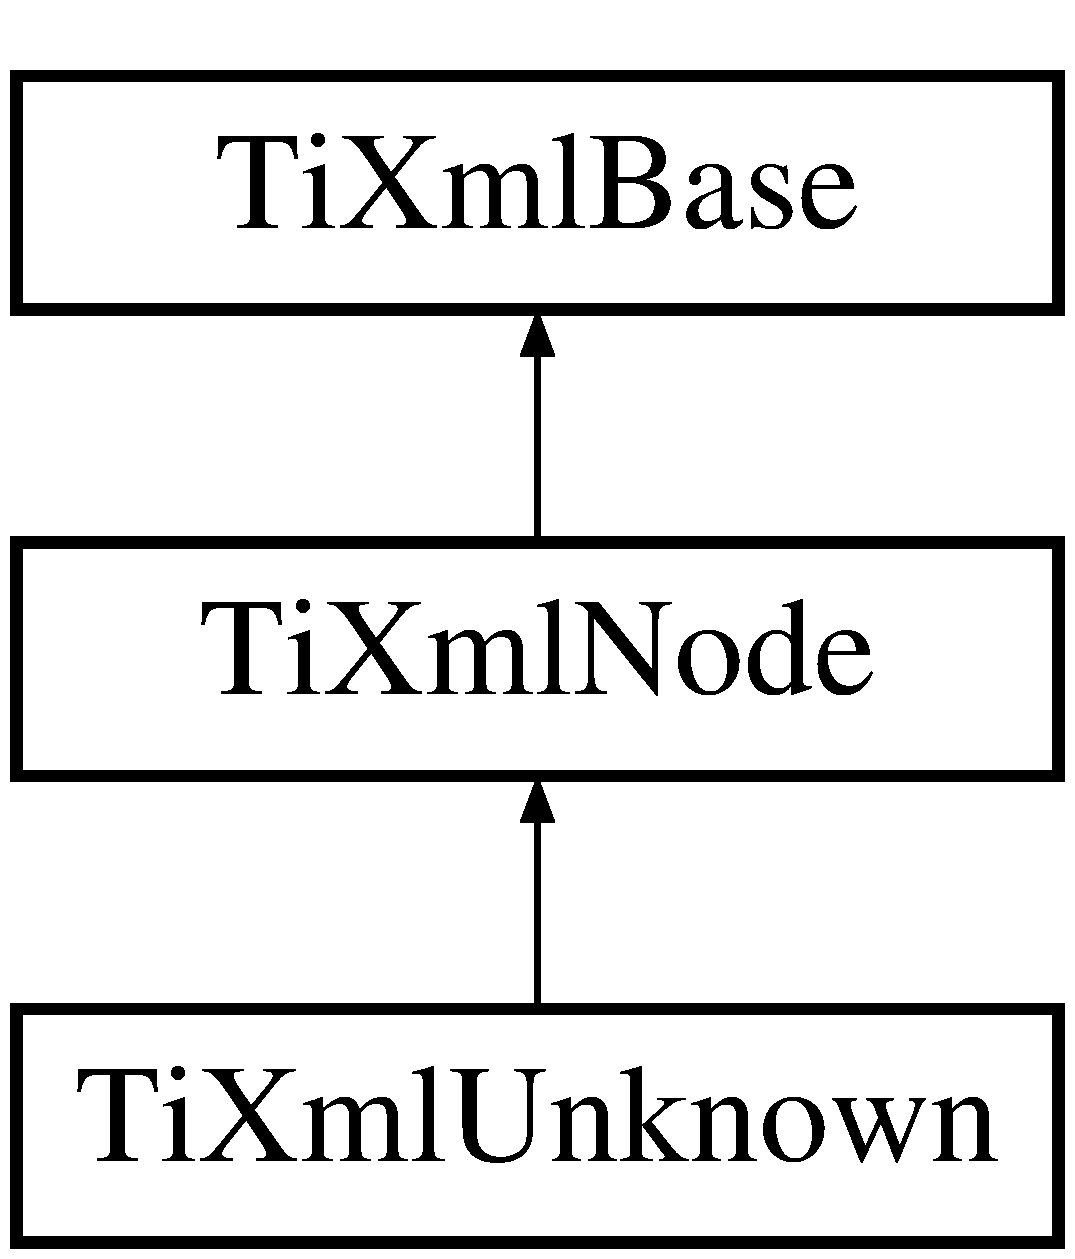
\includegraphics[height=3cm]{classTiXmlUnknown}
\end{center}
\end{figure}


\subsection{Detailed Description}
Any tag that tinyXml doesn't recognize is saved as an unknown. It is a tag of text, but should not be modified. It will be written back to the XML, unchanged, when the file is saved.

DTD tags get thrown into TiXmlUnknowns. \subsection*{Public Member Functions}
\begin{CompactItemize}
\item 
{\bf TiXmlUnknown} ()
\item 
virtual {\bf $\sim$TiXmlUnknown} ()
\item 
{\bf TiXmlUnknown} (const {\bf TiXmlUnknown} \&copy)
\item 
void {\bf operator=} (const {\bf TiXmlUnknown} \&copy)
\item 
virtual {\bf TiXmlNode} $\ast$ {\bf Clone} () const 
\begin{CompactList}\small\item\em Creates a copy of this Unknown and returns it. \item\end{CompactList}\item 
virtual void {\bf Print} (FILE $\ast$cfile, int depth) const 
\item 
virtual const char $\ast$ {\bf Parse} (const char $\ast$p, {\bf TiXmlParsingData} $\ast$data, {\bf TiXmlEncoding} encoding)
\item 
virtual const {\bf TiXmlUnknown} $\ast$ {\bf ToUnknown} () const 
\begin{CompactList}\small\item\em Cast to a more defined type. Will return null not of the requested type. \item\end{CompactList}\item 
virtual {\bf TiXmlUnknown} $\ast$ {\bf ToUnknown} ()
\begin{CompactList}\small\item\em Cast to a more defined type. Will return null not of the requested type. \item\end{CompactList}\item 
virtual bool {\bf Accept} ({\bf TiXmlVisitor} $\ast$content) const 
\end{CompactItemize}
\subsection*{Protected Member Functions}
\begin{CompactItemize}
\item 
void {\bf CopyTo} ({\bf TiXmlUnknown} $\ast$target) const 
\end{CompactItemize}


\subsection{Constructor \& Destructor Documentation}
\index{TiXmlUnknown@{TiXmlUnknown}!TiXmlUnknown@{TiXmlUnknown}}
\index{TiXmlUnknown@{TiXmlUnknown}!TiXmlUnknown@{TiXmlUnknown}}
\subsubsection[TiXmlUnknown]{\setlength{\rightskip}{0pt plus 5cm}TiXmlUnknown::TiXmlUnknown ()\hspace{0.3cm}{\tt  [inline]}}\label{classTiXmlUnknown_945f09b3c6538099c69fc563216750c3}




Referenced by Clone().\index{TiXmlUnknown@{TiXmlUnknown}!$\sim$TiXmlUnknown@{$\sim$TiXmlUnknown}}
\index{$\sim$TiXmlUnknown@{$\sim$TiXmlUnknown}!TiXmlUnknown@{TiXmlUnknown}}
\subsubsection[$\sim$TiXmlUnknown]{\setlength{\rightskip}{0pt plus 5cm}virtual TiXmlUnknown::$\sim$TiXmlUnknown ()\hspace{0.3cm}{\tt  [inline, virtual]}}\label{classTiXmlUnknown_c21966c3b551553d760b4a339c9acda0}


\index{TiXmlUnknown@{TiXmlUnknown}!TiXmlUnknown@{TiXmlUnknown}}
\index{TiXmlUnknown@{TiXmlUnknown}!TiXmlUnknown@{TiXmlUnknown}}
\subsubsection[TiXmlUnknown]{\setlength{\rightskip}{0pt plus 5cm}TiXmlUnknown::TiXmlUnknown (const {\bf TiXmlUnknown} \& {\em copy})\hspace{0.3cm}{\tt  [inline]}}\label{classTiXmlUnknown_be798ff4feea31474850c7f0de6bdf5e}




References CopyTo().

\subsection{Member Function Documentation}
\index{TiXmlUnknown@{TiXmlUnknown}!operator=@{operator=}}
\index{operator=@{operator=}!TiXmlUnknown@{TiXmlUnknown}}
\subsubsection[operator=]{\setlength{\rightskip}{0pt plus 5cm}void TiXmlUnknown::operator= (const {\bf TiXmlUnknown} \& {\em copy})\hspace{0.3cm}{\tt  [inline]}}\label{classTiXmlUnknown_5097fe228cd5ad4edcdddf02c334fd83}




References CopyTo().\index{TiXmlUnknown@{TiXmlUnknown}!Clone@{Clone}}
\index{Clone@{Clone}!TiXmlUnknown@{TiXmlUnknown}}
\subsubsection[Clone]{\setlength{\rightskip}{0pt plus 5cm}{\bf TiXmlNode} $\ast$ TiXmlUnknown::Clone () const\hspace{0.3cm}{\tt  [virtual]}}\label{classTiXmlUnknown_675c4b2684af35e4c7649b7fd5ae598d}


Creates a copy of this Unknown and returns it. 



Implements {\bf TiXmlNode} \doxyref{}{p.}{classTiXmlNode_4508cc3a2d7a98e96a54cc09c37a78a4}.

References CopyTo(), and TiXmlUnknown().\index{TiXmlUnknown@{TiXmlUnknown}!Print@{Print}}
\index{Print@{Print}!TiXmlUnknown@{TiXmlUnknown}}
\subsubsection[Print]{\setlength{\rightskip}{0pt plus 5cm}void TiXmlUnknown::Print (FILE $\ast$ {\em cfile}, \/  int {\em depth}) const\hspace{0.3cm}{\tt  [virtual]}}\label{classTiXmlUnknown_025f19c21ef01ea9be50febb8fe0ba06}


All TinyXml classes can print themselves to a filestream or the string class (\doxyref{TiXmlString}{p.}{classTiXmlString} in non-STL mode, std::string in STL mode.) Either or both cfile and str can be null.

This is a formatted print, and will insert tabs and newlines.

(For an unformatted stream, use the $<$$<$ operator.) 

Implements {\bf TiXmlBase} \doxyref{}{p.}{classTiXmlBase_0de56b3f2ef14c65091a3b916437b512}.

References TiXmlNode::value.\index{TiXmlUnknown@{TiXmlUnknown}!Parse@{Parse}}
\index{Parse@{Parse}!TiXmlUnknown@{TiXmlUnknown}}
\subsubsection[Parse]{\setlength{\rightskip}{0pt plus 5cm}const char $\ast$ TiXmlUnknown::Parse (const char $\ast$ {\em p}, \/  {\bf TiXmlParsingData} $\ast$ {\em data}, \/  {\bf TiXmlEncoding} {\em encoding})\hspace{0.3cm}{\tt  [virtual]}}\label{classTiXmlUnknown_a51c2694e4177b5f0b5429ee5a81b58d}




Implements {\bf TiXmlBase} \doxyref{}{p.}{classTiXmlBase_00e4edb0219d00a1379c856e5a1d2025}.

References TiXmlParsingData::Cursor(), TiXmlNode::GetDocument(), TiXmlBase::location, TiXmlDocument::SetError(), TiXmlBase::SkipWhiteSpace(), TiXmlParsingData::Stamp(), TiXmlBase::TIXML\_\-ERROR\_\-PARSING\_\-UNKNOWN, and TiXmlNode::value.\index{TiXmlUnknown@{TiXmlUnknown}!ToUnknown@{ToUnknown}}
\index{ToUnknown@{ToUnknown}!TiXmlUnknown@{TiXmlUnknown}}
\subsubsection[ToUnknown]{\setlength{\rightskip}{0pt plus 5cm}virtual const {\bf TiXmlUnknown}$\ast$ TiXmlUnknown::ToUnknown () const\hspace{0.3cm}{\tt  [inline, virtual]}}\label{classTiXmlUnknown_b0313e5fe77987d746ac1a97a254419d}


Cast to a more defined type. Will return null not of the requested type. 



Reimplemented from {\bf TiXmlNode} \doxyref{}{p.}{classTiXmlNode_fd7205cf31d7a376929f8a36930627a2}.\index{TiXmlUnknown@{TiXmlUnknown}!ToUnknown@{ToUnknown}}
\index{ToUnknown@{ToUnknown}!TiXmlUnknown@{TiXmlUnknown}}
\subsubsection[ToUnknown]{\setlength{\rightskip}{0pt plus 5cm}virtual {\bf TiXmlUnknown}$\ast$ TiXmlUnknown::ToUnknown ()\hspace{0.3cm}{\tt  [inline, virtual]}}\label{classTiXmlUnknown_67c9fd22940e8c47f706a72cdd2e332c}


Cast to a more defined type. Will return null not of the requested type. 



Reimplemented from {\bf TiXmlNode} \doxyref{}{p.}{classTiXmlNode_06de5af852668c7e4af0d09c205f0b0d}.\index{TiXmlUnknown@{TiXmlUnknown}!Accept@{Accept}}
\index{Accept@{Accept}!TiXmlUnknown@{TiXmlUnknown}}
\subsubsection[Accept]{\setlength{\rightskip}{0pt plus 5cm}bool TiXmlUnknown::Accept ({\bf TiXmlVisitor} $\ast$ {\em content}) const\hspace{0.3cm}{\tt  [virtual]}}\label{classTiXmlUnknown_4e54d7482e05a837cf83c925cc683380}


Walk the XML tree visiting this node and all of its children. 

Implements {\bf TiXmlNode} \doxyref{}{p.}{classTiXmlNode_cc0f88b7462c6cb73809d410a4f5bb86}.

References TiXmlVisitor::Visit().\index{TiXmlUnknown@{TiXmlUnknown}!CopyTo@{CopyTo}}
\index{CopyTo@{CopyTo}!TiXmlUnknown@{TiXmlUnknown}}
\subsubsection[CopyTo]{\setlength{\rightskip}{0pt plus 5cm}void TiXmlUnknown::CopyTo ({\bf TiXmlUnknown} $\ast$ {\em target}) const\hspace{0.3cm}{\tt  [protected]}}\label{classTiXmlUnknown_08ca7b225a2bcb604d3c72e199d33408}




References TiXmlNode::CopyTo().

Referenced by Clone(), operator=(), and TiXmlUnknown().

The documentation for this class was generated from the following files:\begin{CompactItemize}
\item 
{\bf tinyxml.h}\item 
{\bf tinyxml.cpp}\item 
{\bf tinyxmlparser.cpp}\end{CompactItemize}

\section{TiXmlVisitor Class Reference}
\label{classTiXmlVisitor}\index{TiXmlVisitor@{TiXmlVisitor}}
{\tt \#include $<$tinyxml.h$>$}

Inheritance diagram for TiXmlVisitor::\begin{figure}[H]
\begin{center}
\leavevmode
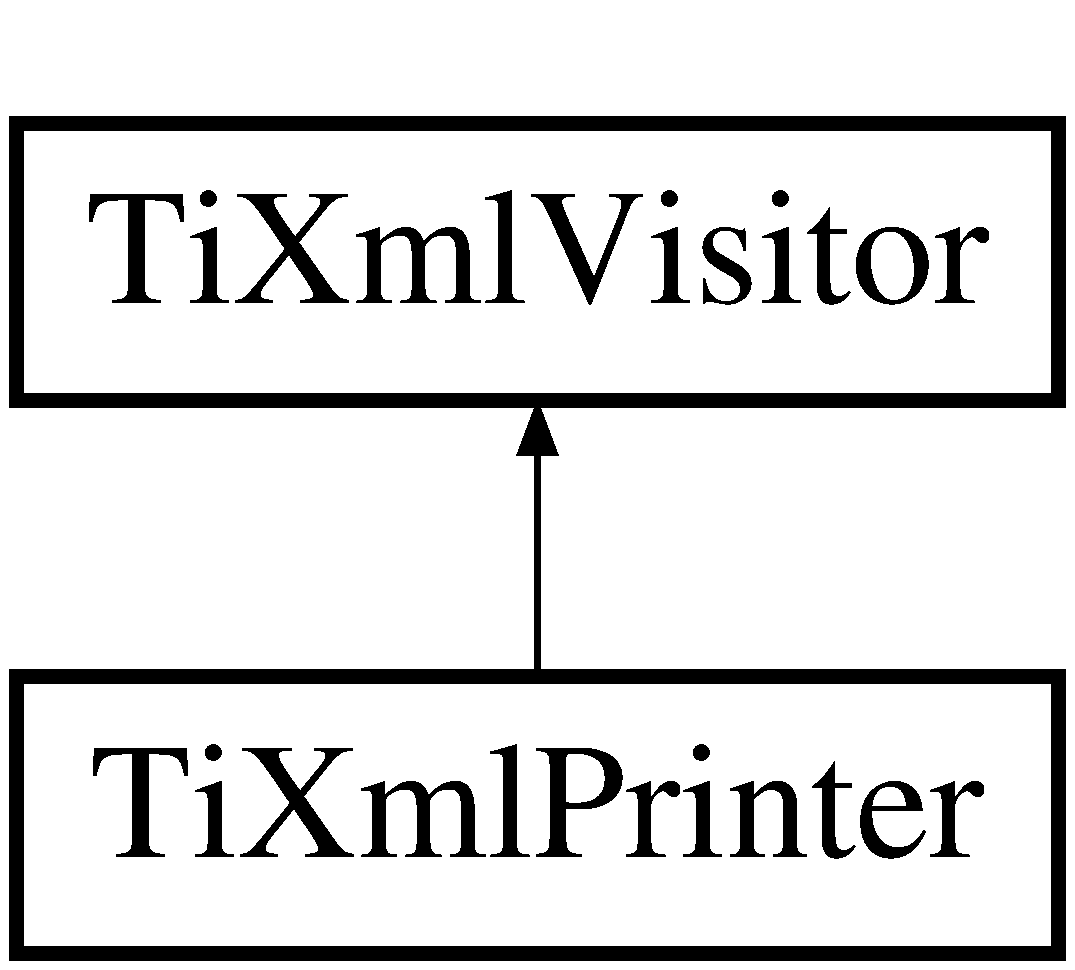
\includegraphics[height=2cm]{classTiXmlVisitor}
\end{center}
\end{figure}


\subsection{Detailed Description}
If you call the Accept() method, it requires being passed a \doxyref{TiXmlVisitor}{p.}{classTiXmlVisitor} class to handle callbacks. For nodes that contain other nodes (Document, Element) you will get called with a VisitEnter/VisitExit pair. Nodes that are always leaves are simple called with \doxyref{Visit()}{p.}{classTiXmlVisitor_fad71c71ce6473fb9b4b64cd92de4a19}.

If you return 'true' from a Visit method, recursive parsing will continue. If you return false, {\bf no children of this node or its sibilings} will be Visited.

All flavors of Visit methods have a default implementation that returns 'true' (continue visiting). You need to only override methods that are interesting to you.

Generally Accept() is called on the \doxyref{TiXmlDocument}{p.}{classTiXmlDocument}, although all nodes suppert Visiting.

You should never change the document from a callback.

\begin{Desc}
\item[See also:]\doxyref{TiXmlNode::Accept()}{p.}{classTiXmlNode_cc0f88b7462c6cb73809d410a4f5bb86} \end{Desc}
\subsection*{Public Member Functions}
\begin{CompactItemize}
\item 
virtual {\bf $\sim$TiXmlVisitor} ()
\item 
virtual bool {\bf VisitEnter} (const {\bf TiXmlDocument} \&)
\begin{CompactList}\small\item\em Visit a document. \item\end{CompactList}\item 
virtual bool {\bf VisitExit} (const {\bf TiXmlDocument} \&)
\begin{CompactList}\small\item\em Visit a document. \item\end{CompactList}\item 
virtual bool {\bf VisitEnter} (const {\bf TiXmlElement} \&, const {\bf TiXmlAttribute} $\ast$)
\begin{CompactList}\small\item\em Visit an element. \item\end{CompactList}\item 
virtual bool {\bf VisitExit} (const {\bf TiXmlElement} \&)
\begin{CompactList}\small\item\em Visit an element. \item\end{CompactList}\item 
virtual bool {\bf Visit} (const {\bf TiXmlDeclaration} \&)
\begin{CompactList}\small\item\em Visit a declaration. \item\end{CompactList}\item 
virtual bool {\bf Visit} (const {\bf TiXmlText} \&)
\begin{CompactList}\small\item\em Visit a text node. \item\end{CompactList}\item 
virtual bool {\bf Visit} (const {\bf TiXmlComment} \&)
\begin{CompactList}\small\item\em Visit a comment node. \item\end{CompactList}\item 
virtual bool {\bf Visit} (const {\bf TiXmlUnknown} \&)
\begin{CompactList}\small\item\em Visit an unknow node. \item\end{CompactList}\end{CompactItemize}


\subsection{Constructor \& Destructor Documentation}
\index{TiXmlVisitor@{TiXmlVisitor}!$\sim$TiXmlVisitor@{$\sim$TiXmlVisitor}}
\index{$\sim$TiXmlVisitor@{$\sim$TiXmlVisitor}!TiXmlVisitor@{TiXmlVisitor}}
\subsubsection[$\sim$TiXmlVisitor]{\setlength{\rightskip}{0pt plus 5cm}virtual TiXmlVisitor::$\sim$TiXmlVisitor ()\hspace{0.3cm}{\tt  [inline, virtual]}}\label{classTiXmlVisitor_276c739ec4701f27c3f86b8ead095e5a}




\subsection{Member Function Documentation}
\index{TiXmlVisitor@{TiXmlVisitor}!VisitEnter@{VisitEnter}}
\index{VisitEnter@{VisitEnter}!TiXmlVisitor@{TiXmlVisitor}}
\subsubsection[VisitEnter]{\setlength{\rightskip}{0pt plus 5cm}virtual bool TiXmlVisitor::VisitEnter (const {\bf TiXmlDocument} \&)\hspace{0.3cm}{\tt  [inline, virtual]}}\label{classTiXmlVisitor_07baecb52dd7d8716ae2a48ad0956ee0}


Visit a document. 



Reimplemented in {\bf TiXmlPrinter} \doxyref{}{p.}{classTiXmlPrinter_2ec73087db26ff4d2c4316c56f861db7}.

Referenced by TiXmlDocument::Accept(), and TiXmlElement::Accept().\index{TiXmlVisitor@{TiXmlVisitor}!VisitExit@{VisitExit}}
\index{VisitExit@{VisitExit}!TiXmlVisitor@{TiXmlVisitor}}
\subsubsection[VisitExit]{\setlength{\rightskip}{0pt plus 5cm}virtual bool TiXmlVisitor::VisitExit (const {\bf TiXmlDocument} \&)\hspace{0.3cm}{\tt  [inline, virtual]}}\label{classTiXmlVisitor_a0ade4f27087447e93974e975c3246ad}


Visit a document. 



Reimplemented in {\bf TiXmlPrinter} \doxyref{}{p.}{classTiXmlPrinter_0a636046fa589b6d7f3e5bd025b3f33e}.

Referenced by TiXmlDocument::Accept(), and TiXmlElement::Accept().\index{TiXmlVisitor@{TiXmlVisitor}!VisitEnter@{VisitEnter}}
\index{VisitEnter@{VisitEnter}!TiXmlVisitor@{TiXmlVisitor}}
\subsubsection[VisitEnter]{\setlength{\rightskip}{0pt plus 5cm}virtual bool TiXmlVisitor::VisitEnter (const {\bf TiXmlElement} \&, \/  const {\bf TiXmlAttribute} $\ast$)\hspace{0.3cm}{\tt  [inline, virtual]}}\label{classTiXmlVisitor_f6c6178ffa517bbdba95d70490875fff}


Visit an element. 



Reimplemented in {\bf TiXmlPrinter} \doxyref{}{p.}{classTiXmlPrinter_6dccaf5ee4979f13877690afe28721e8}.\index{TiXmlVisitor@{TiXmlVisitor}!VisitExit@{VisitExit}}
\index{VisitExit@{VisitExit}!TiXmlVisitor@{TiXmlVisitor}}
\subsubsection[VisitExit]{\setlength{\rightskip}{0pt plus 5cm}virtual bool TiXmlVisitor::VisitExit (const {\bf TiXmlElement} \&)\hspace{0.3cm}{\tt  [inline, virtual]}}\label{classTiXmlVisitor_ec2b1f8116226d52f3a1b95dafd3a32c}


Visit an element. 



Reimplemented in {\bf TiXmlPrinter} \doxyref{}{p.}{classTiXmlPrinter_e6a1df8271df4bf62d7873c38e34aa69}.\index{TiXmlVisitor@{TiXmlVisitor}!Visit@{Visit}}
\index{Visit@{Visit}!TiXmlVisitor@{TiXmlVisitor}}
\subsubsection[Visit]{\setlength{\rightskip}{0pt plus 5cm}virtual bool TiXmlVisitor::Visit (const {\bf TiXmlDeclaration} \&)\hspace{0.3cm}{\tt  [inline, virtual]}}\label{classTiXmlVisitor_fad71c71ce6473fb9b4b64cd92de4a19}


Visit a declaration. 



Reimplemented in {\bf TiXmlPrinter} \doxyref{}{p.}{classTiXmlPrinter_daf7eec4dc43ad071ff52b60361574f5}.

Referenced by TiXmlUnknown::Accept(), TiXmlDeclaration::Accept(), TiXmlText::Accept(), and TiXmlComment::Accept().\index{TiXmlVisitor@{TiXmlVisitor}!Visit@{Visit}}
\index{Visit@{Visit}!TiXmlVisitor@{TiXmlVisitor}}
\subsubsection[Visit]{\setlength{\rightskip}{0pt plus 5cm}virtual bool TiXmlVisitor::Visit (const {\bf TiXmlText} \&)\hspace{0.3cm}{\tt  [inline, virtual]}}\label{classTiXmlVisitor_399b8ebca5cd14664974a32d2ce029e5}


Visit a text node. 



Reimplemented in {\bf TiXmlPrinter} \doxyref{}{p.}{classTiXmlPrinter_0857c5d32c59b9a257f9a49cb9411df5}.\index{TiXmlVisitor@{TiXmlVisitor}!Visit@{Visit}}
\index{Visit@{Visit}!TiXmlVisitor@{TiXmlVisitor}}
\subsubsection[Visit]{\setlength{\rightskip}{0pt plus 5cm}virtual bool TiXmlVisitor::Visit (const {\bf TiXmlComment} \&)\hspace{0.3cm}{\tt  [inline, virtual]}}\label{classTiXmlVisitor_53a60e7a528627b31af3161972cc7fa2}


Visit a comment node. 



Reimplemented in {\bf TiXmlPrinter} \doxyref{}{p.}{classTiXmlPrinter_9870423f5603630e6142f6bdb66dfb57}.\index{TiXmlVisitor@{TiXmlVisitor}!Visit@{Visit}}
\index{Visit@{Visit}!TiXmlVisitor@{TiXmlVisitor}}
\subsubsection[Visit]{\setlength{\rightskip}{0pt plus 5cm}virtual bool TiXmlVisitor::Visit (const {\bf TiXmlUnknown} \&)\hspace{0.3cm}{\tt  [inline, virtual]}}\label{classTiXmlVisitor_7e284d607d275c51dac1adb58159ce28}


Visit an unknow node. 



Reimplemented in {\bf TiXmlPrinter} \doxyref{}{p.}{classTiXmlPrinter_08591a15c9a07afa83c24e08b03d6358}.

The documentation for this class was generated from the following file:\begin{CompactItemize}
\item 
{\bf tinyxml.h}\end{CompactItemize}

\chapter{File Documentation}
\section{agent.cpp File Reference}
\label{agent_8cpp}\index{agent.cpp@{agent.cpp}}


\subsection{Detailed Description}
Implementation of the agent class

\begin{Desc}
\item[Date:]Oct 14th, 2009 last edited: Oct 14th, 2009\end{Desc}
\begin{Desc}
\item[Author:]Michael Sneddon \end{Desc}


{\tt \#include \char`\"{}agent.hh\char`\"{}}\par

\section{agent.hh File Reference}
\label{agent_8hh}\index{agent.hh@{agent.hh}}


\subsection{Detailed Description}
this file contains the interface to the agent class

\begin{Desc}
\item[Date:]Oct 12th, 2009 last edited: Oct 15th, 2009 by Garrit and Michael\end{Desc}
\begin{Desc}
\item[Author:]Garrit Jentsch \end{Desc}


{\tt \#include $<$iostream$>$}\par
{\tt \#include $<$vector$>$}\par
{\tt \#include $<$queue$>$}\par
{\tt \#include \char`\"{}action/arnie.hh\char`\"{}}\par
{\tt \#include \char`\"{}data/data.hh\char`\"{}}\par
{\tt \#include \char`\"{}database/database.hh\char`\"{}}\par
{\tt \#include \char`\"{}message/message.hh\char`\"{}}\par
{\tt \#include \char`\"{}messageGenerator/messagegenerator.hh\char`\"{}}\par
{\tt \#include \char`\"{}../communicator/communicator.hh\char`\"{}}\par
{\tt \#include \char`\"{}../output/outputwriter.hh\char`\"{}}\par
{\tt \#include \char`\"{}../simulators/simulator.hh\char`\"{}}\par
\subsection*{Namespaces}
\begin{CompactItemize}
\item 
namespace {\bf Hive}
\end{CompactItemize}
\subsection*{Classes}
\begin{CompactItemize}
\item 
class {\bf Hive::Agent}
\begin{CompactList}\small\item\em central class of the hive \item\end{CompactList}\end{CompactItemize}

\section{agent\_\-factory.hh File Reference}
\label{agent__factory_8hh}\index{agent\_\-factory.hh@{agent\_\-factory.hh}}


{\tt \#include $<$string$>$}\par
{\tt \#include \char`\"{}../agent.hh\char`\"{}}\par
{\tt \#include \char`\"{}../../input/systemParser/inputsystemreader.hh\char`\"{}}\par
{\tt \#include \char`\"{}../action/arnie.hh\char`\"{}}\par
{\tt \#include \char`\"{}../../simulators/simulator.hh\char`\"{}}\par
{\tt \#include \char`\"{}../../input/system/system.hh\char`\"{}}\par
\subsection*{Namespaces}
\begin{CompactItemize}
\item 
namespace {\bf Hive}
\end{CompactItemize}
\subsection*{Classes}
\begin{CompactItemize}
\item 
class {\bf Hive::AgentFactory}
\begin{CompactList}\small\item\em agent factory \item\end{CompactList}\end{CompactItemize}

\section{arnie.hh File Reference}
\label{arnie_8hh}\index{arnie.hh@{arnie.hh}}


{\tt \#include \char`\"{}../agent.hh\char`\"{}}\par
{\tt \#include \char`\"{}../data/data.hh\char`\"{}}\par
\subsection*{Namespaces}
\begin{CompactItemize}
\item 
namespace {\bf Hive}
\end{CompactItemize}
\subsection*{Classes}
\begin{CompactItemize}
\item 
class {\bf Hive::Action}
\begin{CompactList}\small\item\em action class for working on an agent \item\end{CompactList}\end{CompactItemize}

\section{commandLineParser.cpp File Reference}
\label{commandLineParser_8cpp}\index{commandLineParser.cpp@{commandLineParser.cpp}}


{\tt \#include \char`\"{}commandLineParser.hh\char`\"{}}\par
{\tt \#include $<$iostream$>$}\par
\subsection*{Functions}
\begin{CompactItemize}
\item 
bool {\bf parseArguments} (int argc, const char $\ast$argv[$\,$], map$<$ string, string $>$ \&argMap)
\begin{CompactList}\small\item\em Parses command line arguments from the console into an argMap. \item\end{CompactList}\item 
int {\bf parseAsInt} (map$<$ string, string $>$ \&argMap, string argName, int defaultValue)
\begin{CompactList}\small\item\em Looks up the argument in the argMap and tries to parse the value as an integer. \item\end{CompactList}\item 
double {\bf parseAsDouble} (map$<$ string, string $>$ \&argMap, string argName, double defaultValue)
\begin{CompactList}\small\item\em Looks up the argument in the argMap and tries to parse the value as a double. \item\end{CompactList}\end{CompactItemize}


\subsection{Function Documentation}
\index{commandLineParser.cpp@{commandLineParser.cpp}!parseArguments@{parseArguments}}
\index{parseArguments@{parseArguments}!commandLineParser.cpp@{commandLineParser.cpp}}
\subsubsection[parseArguments]{\setlength{\rightskip}{0pt plus 5cm}bool parseArguments (int {\em argc}, \/  const char $\ast$ {\em argv}[$\,$], \/  std::map$<$ std::string, std::string $>$ \& {\em argMap})}\label{commandLineParser_8cpp_db6c1353f5ffe64f1c40d49ddf1f4b74}


Parses command line arguments from the console into an argMap. 

Given the vector of strings taken from the command line, this function parses out all strings that start with a dash and identifies them as parameters, and attatches the parameter value to whatever string follows. For example, -file help.txt would add an entry to the argMap as a parameter named \char`\"{}file\char`\"{} with value \char`\"{}help.txt\char`\"{}. You can take a look at parseAsInt and parseAsDouble functions that can interpret the value as integers or doubles

\begin{Desc}
\item[Parameters:]
\begin{description}
\item[{\em argc}]the number of arguments \item[{\em argv}]the array of character arrays (strings) \item[{\em argMap}]the map that will be set when this function is called \end{description}
\end{Desc}
\begin{Desc}
\item[Returns:]bool true if successful, false if something went wrong \end{Desc}
\begin{Desc}
\item[Author:]Michael Sneddon \end{Desc}
\index{commandLineParser.cpp@{commandLineParser.cpp}!parseAsDouble@{parseAsDouble}}
\index{parseAsDouble@{parseAsDouble}!commandLineParser.cpp@{commandLineParser.cpp}}
\subsubsection[parseAsDouble]{\setlength{\rightskip}{0pt plus 5cm}double parseAsDouble (map$<$ string, string $>$ \& {\em argMap}, \/  string {\em argName}, \/  double {\em defaultValue})}\label{commandLineParser_8cpp_412e89bbcc308c634d3911a49280bbbc}


Looks up the argument in the argMap and tries to parse the value as a double. 

\begin{Desc}
\item[Parameters:]
\begin{description}
\item[{\em argMap}]the argMap to lookup, generally created by the parseArguments function \item[{\em string}]the name of the parameter to look up \item[{\em defaultValue}]the default value to return if the value was empty \end{description}
\end{Desc}
\begin{Desc}
\item[Returns:]int the parsed double if successful, otherwise the defaultValue given \end{Desc}
\begin{Desc}
\item[Author:]Michael Sneddon \end{Desc}


References Util::convertToDouble().\index{commandLineParser.cpp@{commandLineParser.cpp}!parseAsInt@{parseAsInt}}
\index{parseAsInt@{parseAsInt}!commandLineParser.cpp@{commandLineParser.cpp}}
\subsubsection[parseAsInt]{\setlength{\rightskip}{0pt plus 5cm}int parseAsInt (map$<$ string, string $>$ \& {\em argMap}, \/  string {\em argName}, \/  int {\em defaultValue})}\label{commandLineParser_8cpp_7e2b760fe8b56a663c12352037277dd0}


Looks up the argument in the argMap and tries to parse the value as an integer. 

\begin{Desc}
\item[Parameters:]
\begin{description}
\item[{\em argMap}]the argMap to lookup, generally created by the parseArguments function \item[{\em string}]the name of the parameter to look up \item[{\em defaultValue}]the default value to return if the value was empty \end{description}
\end{Desc}
\begin{Desc}
\item[Returns:]int the parsed int if successful, otherwise the defaultValue given \end{Desc}
\begin{Desc}
\item[Author:]Michael Sneddon \end{Desc}


References Util::convertToInt().
\section{commandLineParser.hh File Reference}
\label{commandLineParser_8hh}\index{commandLineParser.hh@{commandLineParser.hh}}


\subsection{Detailed Description}
Functions to parse command line arguments into a general map that can be accessed later.

\begin{Desc}
\item[Date:]Oct 14th, 2009 last edited: Oct 14th, 2009\end{Desc}
\begin{Desc}
\item[Author:]Michael Sneddon \end{Desc}


{\tt \#include \char`\"{}../../util/util.hh\char`\"{}}\par
{\tt \#include $<$map$>$}\par
{\tt \#include $<$string$>$}\par
\subsection*{Namespaces}
\begin{CompactItemize}
\item 
namespace {\bf Hive}
\end{CompactItemize}
\subsection*{Functions}
\begin{CompactItemize}
\item 
bool {\bf Hive::parseArguments} (int argc, const char $\ast$argv[$\,$], std::map$<$ std::string, std::string $>$ \&argMap)
\begin{CompactList}\small\item\em Parses command line arguments from the console into an argMap. \item\end{CompactList}\item 
int {\bf Hive::parseAsInt} (map$<$ string, string $>$ \&argMap, string argName, int defaultValue)
\begin{CompactList}\small\item\em Looks up the argument in the argMap and tries to parse the value as an integer. \item\end{CompactList}\item 
double {\bf Hive::parseAsDouble} (map$<$ string, string $>$ \&argMap, string argName, double defaultValue)
\begin{CompactList}\small\item\em Looks up the argument in the argMap and tries to parse the value as a double. \item\end{CompactList}\end{CompactItemize}

\section{communicator.hh File Reference}
\label{communicator_8hh}\index{communicator.hh@{communicator.hh}}


\subsection{Detailed Description}
this file contains the interface to the abstract class communicator. Created on: Oct 12, 2009 Author: jentsch

\begin{Desc}
\item[Author:]Garrit Jentsch \end{Desc}
\begin{Desc}
\item[Date:]Oct 12, 2009 last edited: Oct 14, 2009 by Garrit and Michael \end{Desc}


{\tt \#include $<$iostream$>$}\par
{\tt \#include \char`\"{}../agent/message/message.hh\char`\"{}}\par
\subsection*{Namespaces}
\begin{CompactItemize}
\item 
namespace {\bf Hive}
\end{CompactItemize}
\subsection*{Classes}
\begin{CompactItemize}
\item 
class {\bf Hive::Communicator}
\end{CompactItemize}

\section{composer.hh File Reference}
\label{composer_8hh}\index{composer.hh@{composer.hh}}


\subsection{Detailed Description}
this file contains the interface for the composer class.

\begin{Desc}
\item[Author:]Garrit Jentsch\end{Desc}
\begin{Desc}
\item[Date:]13th of Oct, 2009 last edited: Oct 14th, 2009 by Garrit and Michael \end{Desc}


{\tt \#include $<$iostream$>$}\par
{\tt \#include \char`\"{}../agent/agent.hh\char`\"{}}\par
{\tt \#include \char`\"{}../agent/agentFactory/agent\_\-factory.hh\char`\"{}}\par
{\tt \#include \char`\"{}../input/system/system.hh\char`\"{}}\par
\subsection*{Namespaces}
\begin{CompactItemize}
\item 
namespace {\bf Hive}
\end{CompactItemize}
\subsection*{Classes}
\begin{CompactItemize}
\item 
class {\bf Hive::Composer}
\begin{CompactList}\small\item\em this class sets up the entire simulation. \item\end{CompactList}\end{CompactItemize}

\section{constants.hh File Reference}
\label{constants_8hh}\index{constants.hh@{constants.hh}}


\subsection{Detailed Description}
A library of standard constants that are commonly used

\begin{Desc}
\item[Date:]Oct 14th, 2009 last edited: Oct 14th, 2009\end{Desc}
\begin{Desc}
\item[Author:]Michael Sneddon \end{Desc}


\subsection*{Namespaces}
\begin{CompactItemize}
\item 
namespace {\bf Util}
\end{CompactItemize}
\subsection*{Variables}
\begin{CompactItemize}
\item 
const double {\bf Util::PI} = 3.141592653589793
\begin{CompactList}\small\item\em The value of Pi up to 16 significant digits. \item\end{CompactList}\item 
const double {\bf Util::NA} = 6.02214179e23
\begin{CompactList}\small\item\em The value of Avogadro's Number up to 9 significant digits. \item\end{CompactList}\end{CompactItemize}

\section{conversion.cpp File Reference}
\label{conversion_8cpp}\index{conversion.cpp@{conversion.cpp}}


\subsection{Detailed Description}
Implementation of the conversion methods.

\begin{Desc}
\item[Date:]Oct 14th, 2009 last edited: Oct 14th, 2009\end{Desc}
\begin{Desc}
\item[Author:]Michael Sneddon \end{Desc}


{\tt \#include \char`\"{}conversion.hh\char`\"{}}\par
\subsection*{Functions}
\begin{CompactItemize}
\item 
double {\bf Util::convertToDouble} (const std::string \&s)
\begin{CompactList}\small\item\em Parses and converts std::string objects to double values. \item\end{CompactList}\item 
int {\bf Util::convertToInt} (const std::string \&s)
\begin{CompactList}\small\item\em Parses and converts std::string objects to int values. \item\end{CompactList}\item 
string {\bf Util::toString} (double x)
\begin{CompactList}\small\item\em Converts double values to their string representations. \item\end{CompactList}\item 
string {\bf Util::toString} (int x)
\begin{CompactList}\small\item\em Converts integer values to their string representations. \item\end{CompactList}\end{CompactItemize}

\section{conversion.hh File Reference}
\label{conversion_8hh}\index{conversion.hh@{conversion.hh}}


\subsection{Detailed Description}
A library of standard converstions between primitive types and STL objects, such as converting between std::string and double.

\begin{Desc}
\item[Date:]Oct 14th, 2009 last edited: Oct 14th, 2009\end{Desc}
\begin{Desc}
\item[Author:]Michael Sneddon \end{Desc}


{\tt \#include $<$string$>$}\par
{\tt \#include $<$exception$>$}\par
{\tt \#include $<$iostream$>$}\par
{\tt \#include $<$sstream$>$}\par
{\tt \#include $<$stdexcept$>$}\par
{\tt \#include $<$stdlib.h$>$}\par
\subsection*{Namespaces}
\begin{CompactItemize}
\item 
namespace {\bf Util}
\end{CompactItemize}
\subsection*{Functions}
\begin{CompactItemize}
\item 
double {\bf Util::convertToDouble} (const std::string \&s)
\begin{CompactList}\small\item\em Parses and converts std::string objects to double values. \item\end{CompactList}\item 
int {\bf Util::convertToInt} (const std::string \&s)
\begin{CompactList}\small\item\em Parses and converts std::string objects to int values. \item\end{CompactList}\item 
string {\bf Util::toString} (double x)
\begin{CompactList}\small\item\em Converts double values to their string representations. \item\end{CompactList}\item 
string {\bf Util::toString} (int x)
\begin{CompactList}\small\item\em Converts integer values to their string representations. \item\end{CompactList}\end{CompactItemize}

\section{data.hh File Reference}
\label{data_8hh}\index{data.hh@{data.hh}}


\subsection{Detailed Description}
this file contains the interfaces to the classes Data, ...

\begin{Desc}
\item[Date:]Oct 7, 2009 Last edited: Oct 14, 2009 by Garrit and Michael\end{Desc}
\begin{Desc}
\item[Author:]Garrit Jentsch \end{Desc}


{\tt \#include $<$string$>$}\par
\subsection*{Namespaces}
\begin{CompactItemize}
\item 
namespace {\bf Hive}
\end{CompactItemize}
\subsection*{Classes}
\begin{CompactItemize}
\item 
class {\bf Hive::Data}
\begin{CompactList}\small\item\em individual element of the database \item\end{CompactList}\end{CompactItemize}

\section{database.cpp File Reference}
\label{database_8cpp}\index{database.cpp@{database.cpp}}


\subsection{Detailed Description}
This file contains the implementation for the Database class.

\begin{Desc}
\item[Author:]Michael Sneddon\end{Desc}
\begin{Desc}
\item[Date:]Started: Oct 14th, 2009 Last edited: Oct 14th, 2009 \end{Desc}


{\tt \#include \char`\"{}database.hh\char`\"{}}\par

\section{database.hh File Reference}
\label{database_8hh}\index{database.hh@{database.hh}}


\subsection{Detailed Description}
This file contains the specification for the Database class.

\begin{Desc}
\item[Author:]Garrit Jentsch\end{Desc}
\begin{Desc}
\item[Date:]Started: Oct 7th, 2009 Last edited: Oct 14th, 2009 by Garrit and Michael \end{Desc}


{\tt \#include $<$map$>$}\par
{\tt \#include $<$vector$>$}\par
{\tt \#include \char`\"{}../data/data.hh\char`\"{}}\par
{\tt \#include \char`\"{}../../input/dataParser/inputdatareader.hh\char`\"{}}\par
{\tt \#include \char`\"{}../../output/outputwriter.hh\char`\"{}}\par
\subsection*{Namespaces}
\begin{CompactItemize}
\item 
namespace {\bf Hive}
\end{CompactItemize}
\subsection*{Classes}
\begin{CompactItemize}
\item 
class {\bf Hive::Database}
\begin{CompactList}\small\item\em \doxyref{Database}{p.}{classHive_1_1Database} of an agent. \item\end{CompactList}\end{CompactItemize}

\section{dummyagentfactory.cpp File Reference}
\label{dummyagentfactory_8cpp}\index{dummyagentfactory.cpp@{dummyagentfactory.cpp}}


{\tt \#include \char`\"{}dummyagentfactory.hh\char`\"{}}\par
{\tt \#include \char`\"{}../../agent/data/primitive/primitiveData.hh\char`\"{}}\par
{\tt \#include \char`\"{}dummywaveaction.hh\char`\"{}}\par
{\tt \#include \char`\"{}../../communicator/serial/serialcommunicator.hh\char`\"{}}\par
{\tt \#include \char`\"{}../../simulators/dummy/dummySimulator.hh\char`\"{}}\par
{\tt \#include \char`\"{}../../simulators/simulator.hh\char`\"{}}\par
{\tt \#include \char`\"{}dummymessagegenerator.hh\char`\"{}}\par
{\tt \#include $<$string$>$}\par

\section{dummyagentfactory.hh File Reference}
\label{dummyagentfactory_8hh}\index{dummyagentfactory.hh@{dummyagentfactory.hh}}


\subsection{Detailed Description}
this file contains the interface to the dummyagentfactory class

\begin{Desc}
\item[Author:]Garrit Jentsch\end{Desc}
\begin{Desc}
\item[Date:]Oct 14th, 2009 last edited Oct 15th, 2009 by Garrit \end{Desc}


{\tt \#include \char`\"{}../../agent/agentFactory/agent\_\-factory.hh\char`\"{}}\par
\subsection*{Namespaces}
\begin{CompactItemize}
\item 
namespace {\bf Dummy}
\end{CompactItemize}
\subsection*{Classes}
\begin{CompactItemize}
\item 
class {\bf Dummy::DummyAgentFactory}
\begin{CompactList}\small\item\em simple implementation of an agentfactory \item\end{CompactList}\end{CompactItemize}

\section{dummyComposer.cpp File Reference}
\label{dummyComposer_8cpp}\index{dummyComposer.cpp@{dummyComposer.cpp}}


{\tt \#include \char`\"{}dummycomposer.hh\char`\"{}}\par

\section{dummycomposer.hh File Reference}
\label{dummycomposer_8hh}\index{dummycomposer.hh@{dummycomposer.hh}}


{\tt \#include \char`\"{}../../composer/composer.hh\char`\"{}}\par
{\tt \#include \char`\"{}dummyagentfactory.hh\char`\"{}}\par
{\tt \#include \char`\"{}dummywaveaction.hh\char`\"{}}\par
{\tt \#include \char`\"{}../../agent/data/primitive/primitiveData.hh\char`\"{}}\par
{\tt \#include \char`\"{}../../communicator/serial/serialcommunicator.hh\char`\"{}}\par
\subsection*{Namespaces}
\begin{CompactItemize}
\item 
namespace {\bf Dummy}
\end{CompactItemize}
\subsection*{Classes}
\begin{CompactItemize}
\item 
class {\bf Dummy::DummyComposer}
\end{CompactItemize}

\section{dummymessagegenerator.cpp File Reference}
\label{dummymessagegenerator_8cpp}\index{dummymessagegenerator.cpp@{dummymessagegenerator.cpp}}


{\tt \#include \char`\"{}dummymessagegenerator.hh\char`\"{}}\par

\section{dummymessagegenerator.hh File Reference}
\label{dummymessagegenerator_8hh}\index{dummymessagegenerator.hh@{dummymessagegenerator.hh}}


\subsection{Detailed Description}
this file contains the interface to the dummymessagegenerator

\begin{Desc}
\item[Author:]garrit jentsch\end{Desc}
\begin{Desc}
\item[Date:]Oct 15, 2009, last edited 10-15-2009 \end{Desc}


{\tt \#include \char`\"{}../../agent/messageGenerator/messagegenerator.hh\char`\"{}}\par
{\tt \#include \char`\"{}../../agent/data/primitive/primitiveData.hh\char`\"{}}\par
\subsection*{Namespaces}
\begin{CompactItemize}
\item 
namespace {\bf Dummy}
\end{CompactItemize}
\subsection*{Classes}
\begin{CompactItemize}
\item 
class {\bf Dummy::DummyMessageGenerator}
\begin{CompactList}\small\item\em this class implements the messagegenerator \item\end{CompactList}\end{CompactItemize}

\section{dummySimulator.cpp File Reference}
\label{dummySimulator_8cpp}\index{dummySimulator.cpp@{dummySimulator.cpp}}


{\tt \#include \char`\"{}dummySimulator.hh\char`\"{}}\par

\section{dummySimulator.hh File Reference}
\label{dummySimulator_8hh}\index{dummySimulator.hh@{dummySimulator.hh}}


{\tt \#include \char`\"{}../simulator.hh\char`\"{}}\par
{\tt \#include \char`\"{}../../agent/data/primitive/primitiveData.hh\char`\"{}}\par
{\tt \#include \char`\"{}../../util/util.hh\char`\"{}}\par
\subsection*{Namespaces}
\begin{CompactItemize}
\item 
namespace {\bf Hive}
\end{CompactItemize}
\subsection*{Classes}
\begin{CompactItemize}
\item 
class {\bf Hive::DummySimulator}
\end{CompactItemize}

\section{dummywaveaction.cpp File Reference}
\label{dummywaveaction_8cpp}\index{dummywaveaction.cpp@{dummywaveaction.cpp}}


{\tt \#include \char`\"{}dummywaveaction.hh\char`\"{}}\par
{\tt \#include \char`\"{}../../agent/data/primitive/primitiveData.hh\char`\"{}}\par
{\tt \#include $<$stdlib.h$>$}\par

\section{dummywaveaction.hh File Reference}
\label{dummywaveaction_8hh}\index{dummywaveaction.hh@{dummywaveaction.hh}}


\subsection{Detailed Description}
this file contains the interface of the dummywaveaction

\begin{Desc}
\item[Date:]Oct 14, 2009 last edited 10-15-2009\end{Desc}
\begin{Desc}
\item[Author:]garrit jentsch \end{Desc}


{\tt \#include \char`\"{}../../agent/action/arnie.hh\char`\"{}}\par
\subsection*{Namespaces}
\begin{CompactItemize}
\item 
namespace {\bf Dummy}
\end{CompactItemize}
\subsection*{Classes}
\begin{CompactItemize}
\item 
class {\bf Dummy::DummyWaveAction}
\begin{CompactList}\small\item\em this is a dummy implementation of the action class \item\end{CompactList}\end{CompactItemize}

\section{exception.hh File Reference}
\label{exception_8hh}\index{exception.hh@{exception.hh}}



\section{hive.cpp File Reference}
\label{hive_8cpp}\index{hive.cpp@{hive.cpp}}


\subsection{Detailed Description}
The main entry point for hive. 

This file contains the main function and some other things.

\begin{Desc}
\item[Author:]Michael Sneddon \end{Desc}
\begin{Desc}
\item[Date:]Started: Oct 7, 2009 Last edited: Oct 14, 2009 by Michael and Garrit\end{Desc}
\begin{Desc}
\item[{\bf Todo}]Fill in the details.\end{Desc}


{\tt \#include $<$iostream$>$}\par
{\tt \#include $<$string$>$}\par
{\tt \#include $<$time.h$>$}\par
{\tt \#include \char`\"{}agent/agent.hh\char`\"{}}\par
{\tt \#include \char`\"{}projects/dummyAgent/dummycomposer.hh\char`\"{}}\par
\subsection*{Functions}
\begin{CompactItemize}
\item 
int {\bf main} (int argc, char $\ast$argv[$\,$])
\end{CompactItemize}


\subsection{Function Documentation}
\index{hive.cpp@{hive.cpp}!main@{main}}
\index{main@{main}!hive.cpp@{hive.cpp}}
\subsubsection[main]{\setlength{\rightskip}{0pt plus 5cm}int main (int {\em argc}, \/  char $\ast$ {\em argv}[$\,$])}\label{hive_8cpp_0ddf1224851353fc92bfbff6f499fa97}


Main method for hive.

\begin{Desc}
\item[Parameters:]
\begin{description}
\item[{\em argc}]number of arguments (this is the length of argv) \item[{\em argv\mbox{[}$\,$\mbox{]}}]pointer to char arrays (strings) that were passed as arguments \end{description}
\end{Desc}
\begin{Desc}
\item[Returns:]zero if hive ran successfully, an error code if it did not \end{Desc}


References Hive::Composer::getTopLevelAgent(), Hive::Agent::propagate(), and Hive::Composer::setupSimulation().
\section{hive.hh File Reference}
\label{hive_8hh}\index{hive.hh@{hive.hh}}


\subsection{Detailed Description}
The main header file for hive. 

This file contains the main function headers and declarations.

\begin{Desc}
\item[Author:]Michael Sneddon \end{Desc}
\begin{Desc}
\item[Date:]Started: Oct 14, 2009 Last edited: Oct 14, 2009\end{Desc}
\begin{Desc}
\item[{\bf Todo}]Fill in the details.\end{Desc}


{\tt \#include $<$stdlib.h$>$}\par
\subsection*{Namespaces}
\begin{CompactItemize}
\item 
namespace {\bf Hive}
\end{CompactItemize}

\section{inputdatareader.hh File Reference}
\label{inputdatareader_8hh}\index{inputdatareader.hh@{inputdatareader.hh}}


\subsection{Detailed Description}
this file contains the interface for the class inputreader

\begin{Desc}
\item[Author:]Garrit Jentsch\end{Desc}
\begin{Desc}
\item[Date:]Oct 13, 2009 last edited: Oct 13, 2009 by Garrit \end{Desc}


{\tt \#include $<$fstream$>$}\par
{\tt \#include $<$iostream$>$}\par
{\tt \#include \char`\"{}../../agent/data/data.hh\char`\"{}}\par
\subsection*{Namespaces}
\begin{CompactItemize}
\item 
namespace {\bf Hive}
\end{CompactItemize}
\subsection*{Classes}
\begin{CompactItemize}
\item 
class {\bf Hive::InputDataReader}
\begin{CompactList}\small\item\em reads input from filestream \item\end{CompactList}\end{CompactItemize}

\section{inputsystemreader.hh File Reference}
\label{inputsystemreader_8hh}\index{inputsystemreader.hh@{inputsystemreader.hh}}


{\tt \#include $<$fstream$>$}\par
{\tt \#include $<$iostream$>$}\par
{\tt \#include \char`\"{}../system/system.hh\char`\"{}}\par
\subsection*{Namespaces}
\begin{CompactItemize}
\item 
namespace {\bf Hive}
\end{CompactItemize}
\subsection*{Classes}
\begin{CompactItemize}
\item 
class {\bf Hive::InputSystemReader}
\begin{CompactList}\small\item\em abstract class for reading a system \item\end{CompactList}\end{CompactItemize}

\section{message.cpp File Reference}
\label{message_8cpp}\index{message.cpp@{message.cpp}}


{\tt \#include \char`\"{}message.hh\char`\"{}}\par

\section{message.hh File Reference}
\label{message_8hh}\index{message.hh@{message.hh}}


{\tt \#include $<$vector$>$}\par
{\tt \#include \char`\"{}../data/data.hh\char`\"{}}\par
{\tt \#include \char`\"{}../agent.hh\char`\"{}}\par
\subsection*{Namespaces}
\begin{CompactItemize}
\item 
namespace {\bf Hive}
\end{CompactItemize}
\subsection*{Classes}
\begin{CompactItemize}
\item 
class {\bf Hive::Message}
\begin{CompactList}\small\item\em message for agent communication. \item\end{CompactList}\end{CompactItemize}

\section{messagegenerator.hh File Reference}
\label{messagegenerator_8hh}\index{messagegenerator.hh@{messagegenerator.hh}}


{\tt \#include \char`\"{}../agent.hh\char`\"{}}\par
{\tt \#include \char`\"{}../message/message.hh\char`\"{}}\par
\subsection*{Namespaces}
\begin{CompactItemize}
\item 
namespace {\bf Hive}
\end{CompactItemize}
\subsection*{Classes}
\begin{CompactItemize}
\item 
class {\bf Hive::MessageGenerator}
\end{CompactItemize}

\section{mtrand.cpp File Reference}
\label{mtrand_8cpp}\index{mtrand.cpp@{mtrand.cpp}}


{\tt \#include \char`\"{}mtrand.h\char`\"{}}\par

\section{mtrand.h File Reference}
\label{mtrand_8h}\index{mtrand.h@{mtrand.h}}


\subsection*{Classes}
\begin{CompactItemize}
\item 
class {\bf MTRand\_\-int32}
\item 
class {\bf MTRand}
\item 
class {\bf MTRand\_\-closed}
\item 
class {\bf MTRand\_\-open}
\item 
class {\bf MTRand53}
\end{CompactItemize}

\section{muParser.cpp File Reference}
\label{muParser_8cpp}\index{muParser.cpp@{muParser.cpp}}


\subsection{Detailed Description}
Implementation of the standard floating point parser. 



{\tt \#include \char`\"{}muParser.h\char`\"{}}\par
{\tt \#include $<$cmath$>$}\par
{\tt \#include $<$algorithm$>$}\par
{\tt \#include $<$numeric$>$}\par
\subsection*{Namespaces}
\begin{CompactItemize}
\item 
namespace {\bf mu}
\end{CompactItemize}
\subsection*{Defines}
\begin{CompactItemize}
\item 
\#define {\bf PARSER\_\-CONST\_\-PI}~3.141592653589793238462643
\begin{CompactList}\small\item\em Pi (what else?). \item\end{CompactList}\item 
\#define {\bf PARSER\_\-CONST\_\-E}~2.718281828459045235360287
\begin{CompactList}\small\item\em The eulerian number. \item\end{CompactList}\end{CompactItemize}


\subsection{Define Documentation}
\index{muParser.cpp@{muParser.cpp}!PARSER\_\-CONST\_\-E@{PARSER\_\-CONST\_\-E}}
\index{PARSER\_\-CONST\_\-E@{PARSER\_\-CONST\_\-E}!muParser.cpp@{muParser.cpp}}
\subsubsection[PARSER\_\-CONST\_\-E]{\setlength{\rightskip}{0pt plus 5cm}\#define PARSER\_\-CONST\_\-E~2.718281828459045235360287}\label{muParser_8cpp_4ab603294085c34e8c659fa4e84d7e8c}


The eulerian number. 



Referenced by mu::Parser::InitConst().\index{muParser.cpp@{muParser.cpp}!PARSER\_\-CONST\_\-PI@{PARSER\_\-CONST\_\-PI}}
\index{PARSER\_\-CONST\_\-PI@{PARSER\_\-CONST\_\-PI}!muParser.cpp@{muParser.cpp}}
\subsubsection[PARSER\_\-CONST\_\-PI]{\setlength{\rightskip}{0pt plus 5cm}\#define PARSER\_\-CONST\_\-PI~3.141592653589793238462643}\label{muParser_8cpp_63af9517c2e94ffd215fea964afb162c}


Pi (what else?). 



Referenced by mu::Parser::InitConst().
\section{muParser.h File Reference}
\label{muParser_8h}\index{muParser.h@{muParser.h}}


\subsection{Detailed Description}
Definition of the standard floating point parser. 



{\tt \#include $<$vector$>$}\par
{\tt \#include $<$locale$>$}\par
{\tt \#include \char`\"{}muParserBase.h\char`\"{}}\par
\subsection*{Namespaces}
\begin{CompactItemize}
\item 
namespace {\bf mu}
\end{CompactItemize}
\subsection*{Classes}
\begin{CompactItemize}
\item 
class {\bf mu::Parser}
\begin{CompactList}\small\item\em Mathematical expressions parser. \item\end{CompactList}\item 
class \textbf{mu::Parser::change\_\-dec\_\-sep$<$ TChar $>$}
\begin{CompactList}\small\item\em A facet class used to change decimal and thousands separator. \item\end{CompactList}\end{CompactItemize}

\section{muParserBase.cpp File Reference}
\label{muParserBase_8cpp}\index{muParserBase.cpp@{muParserBase.cpp}}


\subsection{Detailed Description}
This file contains the basic implementation of the muparser engine. 



{\tt \#include \char`\"{}muParser.h\char`\"{}}\par
{\tt \#include $<$cassert$>$}\par
{\tt \#include $<$cmath$>$}\par
{\tt \#include $<$memory$>$}\par
{\tt \#include $<$vector$>$}\par
{\tt \#include $<$deque$>$}\par
{\tt \#include $<$sstream$>$}\par
{\tt \#include $<$locale$>$}\par
\subsection*{Namespaces}
\begin{CompactItemize}
\item 
namespace {\bf mu}
\end{CompactItemize}

\section{muParserBase.h File Reference}
\label{muParserBase_8h}\index{muParserBase.h@{muParserBase.h}}


\subsection{Detailed Description}
This file contains the class definition of the muparser engine. 



{\tt \#include $<$cmath$>$}\par
{\tt \#include $<$string$>$}\par
{\tt \#include $<$iostream$>$}\par
{\tt \#include $<$map$>$}\par
{\tt \#include $<$memory$>$}\par
{\tt \#include \char`\"{}muParserDef.h\char`\"{}}\par
{\tt \#include \char`\"{}muParserStack.h\char`\"{}}\par
{\tt \#include \char`\"{}muParserTokenReader.h\char`\"{}}\par
{\tt \#include \char`\"{}muParserBytecode.h\char`\"{}}\par
{\tt \#include \char`\"{}muParserError.h\char`\"{}}\par
\subsection*{Namespaces}
\begin{CompactItemize}
\item 
namespace {\bf mu}
\end{CompactItemize}
\subsection*{Classes}
\begin{CompactItemize}
\item 
class {\bf mu::ParserBase}
\begin{CompactList}\small\item\em Mathematical expressions parser (base parser engine). \item\end{CompactList}\end{CompactItemize}
\subsection*{Defines}
\begin{CompactItemize}
\item 
\#define {\bf MUP\_\-DEFINE\_\-FUNC}(TYPE)
\end{CompactItemize}


\subsection{Define Documentation}
\index{muParserBase.h@{muParserBase.h}!MUP\_\-DEFINE\_\-FUNC@{MUP\_\-DEFINE\_\-FUNC}}
\index{MUP\_\-DEFINE\_\-FUNC@{MUP\_\-DEFINE\_\-FUNC}!muParserBase.h@{muParserBase.h}}
\subsubsection[MUP\_\-DEFINE\_\-FUNC]{\setlength{\rightskip}{0pt plus 5cm}\#define MUP\_\-DEFINE\_\-FUNC(TYPE)}\label{muParserBase_8h_f2dfa18864cf91426f80969960372761}


\textbf{Value:}

\begin{Code}\begin{verbatim}inline void DefineFun(const string_type &a_strName, TYPE a_pFun, bool a_bAllowOpt = true)  \
    {                                                                                   \
      AddCallback( a_strName, ParserCallback(a_pFun, a_bAllowOpt),                      \
                   m_FunDef, ValidNameChars() );                                        \
    }
\end{verbatim}
\end{Code}

\section{muParserBytecode.cpp File Reference}
\label{muParserBytecode_8cpp}\index{muParserBytecode.cpp@{muParserBytecode.cpp}}


\subsection{Detailed Description}
Implementation of the parser bytecode class. 



{\tt \#include \char`\"{}muParserBytecode.h\char`\"{}}\par
{\tt \#include $<$cassert$>$}\par
{\tt \#include $<$string$>$}\par
{\tt \#include $<$stack$>$}\par
{\tt \#include $<$vector$>$}\par
{\tt \#include $<$iostream$>$}\par
{\tt \#include \char`\"{}muParserDef.h\char`\"{}}\par
{\tt \#include \char`\"{}muParserError.h\char`\"{}}\par
{\tt \#include \char`\"{}muParserToken.h\char`\"{}}\par
\subsection*{Namespaces}
\begin{CompactItemize}
\item 
namespace {\bf mu}
\end{CompactItemize}

\section{muParserBytecode.h File Reference}
\label{muParserBytecode_8h}\index{muParserBytecode.h@{muParserBytecode.h}}


\subsection{Detailed Description}
Definition of the parser bytecode class. 



{\tt \#include $<$cassert$>$}\par
{\tt \#include $<$string$>$}\par
{\tt \#include $<$stack$>$}\par
{\tt \#include $<$vector$>$}\par
{\tt \#include \char`\"{}muParserDef.h\char`\"{}}\par
{\tt \#include \char`\"{}muParserError.h\char`\"{}}\par
{\tt \#include \char`\"{}muParserToken.h\char`\"{}}\par
\subsection*{Namespaces}
\begin{CompactItemize}
\item 
namespace {\bf mu}
\end{CompactItemize}
\subsection*{Classes}
\begin{CompactItemize}
\item 
class {\bf mu::ParserByteCode}
\begin{CompactList}\small\item\em Bytecode implementation of the Math \doxyref{Parser}{p.}{classmu_1_1Parser}. \item\end{CompactList}\end{CompactItemize}

\section{muParserCallback.cpp File Reference}
\label{muParserCallback_8cpp}\index{muParserCallback.cpp@{muParserCallback.cpp}}


\subsection{Detailed Description}
Implementation of the parser callback class. 



{\tt \#include \char`\"{}muParserCallback.h\char`\"{}}\par
\subsection*{Namespaces}
\begin{CompactItemize}
\item 
namespace {\bf mu}
\end{CompactItemize}

\section{muParserCallback.h File Reference}
\label{muParserCallback_8h}\index{muParserCallback.h@{muParserCallback.h}}


\subsection{Detailed Description}
Definition of the parser callback class. 



{\tt \#include \char`\"{}muParserDef.h\char`\"{}}\par
\subsection*{Namespaces}
\begin{CompactItemize}
\item 
namespace {\bf mu}
\end{CompactItemize}
\subsection*{Classes}
\begin{CompactItemize}
\item 
class {\bf mu::ParserCallback}
\begin{CompactList}\small\item\em Encapsulation of prototypes for a numerical parser function. \item\end{CompactList}\end{CompactItemize}
\subsection*{Typedefs}
\begin{CompactItemize}
\item 
typedef std::map$<$ string\_\-type, ParserCallback $>$ {\bf mu::funmap\_\-type}
\begin{CompactList}\small\item\em Container for Callback objects. \item\end{CompactList}\end{CompactItemize}

\section{muParserComplex.cpp File Reference}
\label{muParserComplex_8cpp}\index{muParserComplex.cpp@{muParserComplex.cpp}}


\subsection{Detailed Description}
This file contains the implementation of a parser using complex numbers. 



{\tt \#include \char`\"{}muParserComplex.h\char`\"{}}\par
{\tt \#include $<$cmath$>$}\par
{\tt \#include $<$complex$>$}\par
{\tt \#include $<$algorithm$>$}\par
{\tt \#include $<$numeric$>$}\par
\subsection*{Namespaces}
\begin{CompactItemize}
\item 
namespace {\bf mu}
\end{CompactItemize}

\section{muParserComplex.h File Reference}
\label{muParserComplex_8h}\index{muParserComplex.h@{muParserComplex.h}}


\subsection{Detailed Description}
This file contains a definition of a parser using complex numbers. 



{\tt \#include \char`\"{}muParserBase.h\char`\"{}}\par
{\tt \#include $<$vector$>$}\par
{\tt \#include $<$complex$>$}\par
\subsection*{Namespaces}
\begin{CompactItemize}
\item 
namespace {\bf mu}
\end{CompactItemize}
\subsection*{Classes}
\begin{CompactItemize}
\item 
class {\bf mu::ParserComplex}
\begin{CompactList}\small\item\em Mathematical expressions parser. \item\end{CompactList}\end{CompactItemize}

\section{muParserDef.h File Reference}
\label{muParserDef_8h}\index{muParserDef.h@{muParserDef.h}}


\subsection{Detailed Description}
This file contains standard definitions used by the parser. 



{\tt \#include $<$iostream$>$}\par
{\tt \#include $<$string$>$}\par
{\tt \#include $<$sstream$>$}\par
{\tt \#include $<$map$>$}\par
{\tt \#include \char`\"{}muParserFixes.h\char`\"{}}\par
\subsection*{Namespaces}
\begin{CompactItemize}
\item 
namespace {\bf mu}
\end{CompactItemize}
\subsection*{Classes}
\begin{CompactItemize}
\item 
struct {\bf mu::STATIC\_\-ASSERTION\_\-FAILURE$<$ true $>$}
\end{CompactItemize}
\subsection*{Defines}
\begin{CompactItemize}
\item 
\#define {\bf MUP\_\-BASETYPE}~double
\begin{CompactList}\small\item\em Define the base datatype for values. \item\end{CompactList}\item 
\#define {\bf MUP\_\-BYTECODE\_\-TYPE}~long
\begin{CompactList}\small\item\em Definition of the basic bytecode datatype. \item\end{CompactList}\item 
\#define {\bf MUP\_\-STRING\_\-TYPE}~std::string
\begin{CompactList}\small\item\em Definition of the basic parser string type. \item\end{CompactList}\item 
\#define {\bf MUP\_\-FAIL}(MSG)
\item 
\#define {\bf MUP\_\-ASSERT}(COND)
\end{CompactItemize}
\subsection*{Typedefs}
\begin{CompactItemize}
\item 
typedef MUP\_\-BASETYPE {\bf mu::value\_\-type}
\begin{CompactList}\small\item\em The numeric datatype used by the parser. \item\end{CompactList}\item 
typedef MUP\_\-STRING\_\-TYPE {\bf mu::string\_\-type}
\begin{CompactList}\small\item\em The stringtype used by the parser. \item\end{CompactList}\item 
typedef MUP\_\-BYTECODE\_\-TYPE {\bf mu::bytecode\_\-type}
\begin{CompactList}\small\item\em The bytecode type used by the parser. \item\end{CompactList}\item 
typedef string\_\-type::value\_\-type {\bf mu::char\_\-type}
\begin{CompactList}\small\item\em The character type used by the parser. \item\end{CompactList}\item 
typedef std::basic\_\-stringstream$<$ char\_\-type, std::char\_\-traits$<$ char\_\-type $>$, std::allocator$<$ char\_\-type $>$ $>$ {\bf mu::stringstream\_\-type}
\begin{CompactList}\small\item\em Typedef for easily using stringstream that respect the parser stringtype. \item\end{CompactList}\item 
typedef std::map$<$ string\_\-type, value\_\-type $\ast$ $>$ {\bf mu::varmap\_\-type}
\begin{CompactList}\small\item\em Type used for storing variables. \item\end{CompactList}\item 
typedef std::map$<$ string\_\-type, value\_\-type $>$ {\bf mu::valmap\_\-type}
\begin{CompactList}\small\item\em Type used for storing constants. \item\end{CompactList}\item 
typedef std::map$<$ string\_\-type, std::size\_\-t $>$ {\bf mu::strmap\_\-type}
\begin{CompactList}\small\item\em Type for assigning a string name to an index in the internal string table. \item\end{CompactList}\item 
typedef value\_\-type($\ast$ {\bf mu::fun\_\-type0} )()
\begin{CompactList}\small\item\em Callback type used for functions without arguments. \item\end{CompactList}\item 
typedef value\_\-type($\ast$ {\bf mu::fun\_\-type1} )(value\_\-type)
\begin{CompactList}\small\item\em Callback type used for functions with a single arguments. \item\end{CompactList}\item 
typedef value\_\-type($\ast$ {\bf mu::fun\_\-type2} )(value\_\-type, value\_\-type)
\begin{CompactList}\small\item\em Callback type used for functions with two arguments. \item\end{CompactList}\item 
typedef value\_\-type($\ast$ {\bf mu::fun\_\-type3} )(value\_\-type, value\_\-type, value\_\-type)
\begin{CompactList}\small\item\em Callback type used for functions with three arguments. \item\end{CompactList}\item 
typedef value\_\-type($\ast$ {\bf mu::fun\_\-type4} )(value\_\-type, value\_\-type, value\_\-type, value\_\-type)
\begin{CompactList}\small\item\em Callback type used for functions with four arguments. \item\end{CompactList}\item 
typedef value\_\-type($\ast$ {\bf mu::fun\_\-type5} )(value\_\-type, value\_\-type, value\_\-type, value\_\-type, value\_\-type)
\begin{CompactList}\small\item\em Callback type used for functions with five arguments. \item\end{CompactList}\item 
typedef value\_\-type($\ast$ {\bf mu::multfun\_\-type} )(const value\_\-type $\ast$, int)
\begin{CompactList}\small\item\em Callback type used for functions with a variable argument list. \item\end{CompactList}\item 
typedef value\_\-type($\ast$ {\bf mu::strfun\_\-type1} )(const char\_\-type $\ast$)
\begin{CompactList}\small\item\em Callback type used for functions taking a string as an argument. \item\end{CompactList}\item 
typedef value\_\-type($\ast$ {\bf mu::strfun\_\-type2} )(const char\_\-type $\ast$, value\_\-type)
\begin{CompactList}\small\item\em Callback type used for functions taking a string and a value as arguments. \item\end{CompactList}\item 
typedef value\_\-type($\ast$ {\bf mu::strfun\_\-type3} )(const char\_\-type $\ast$, value\_\-type, value\_\-type)
\begin{CompactList}\small\item\em Callback type used for functions taking a string and two values as arguments. \item\end{CompactList}\item 
typedef int($\ast$ {\bf mu::identfun\_\-type} )(const char\_\-type $\ast$sExpr, int $\ast$nPos, value\_\-type $\ast$fVal)
\begin{CompactList}\small\item\em Callback used for functions that identify values in a string. \item\end{CompactList}\item 
typedef value\_\-type $\ast$($\ast$ {\bf mu::facfun\_\-type} )(const char\_\-type $\ast$, void $\ast$)
\begin{CompactList}\small\item\em Callback used for variable creation factory functions. \item\end{CompactList}\item 
typedef char {\bf mu::MAP\_\-TYPE\_\-CANT\_\-BE\_\-UNSIGNED} [sizeof(STATIC\_\-ASSERTION\_\-FAILURE$<$ bytecode\_\-type(-1)$<$ 0 $>$)]
\begin{CompactList}\small\item\em This is a static typecheck. \item\end{CompactList}\end{CompactItemize}
\subsection*{Enumerations}
\begin{CompactItemize}
\item 
enum {\bf mu::ECmdCode} \{ \par
{\bf mu::cmLE} =  0, 
{\bf mu::cmGE} =  1, 
{\bf mu::cmNEQ} =  2, 
{\bf mu::cmEQ} =  3, 
\par
{\bf mu::cmLT} =  4, 
{\bf mu::cmGT} =  5, 
{\bf mu::cmADD} =  6, 
{\bf mu::cmSUB} =  7, 
\par
{\bf mu::cmMUL} =  8, 
{\bf mu::cmDIV} =  9, 
{\bf mu::cmPOW} =  10, 
{\bf mu::cmAND} =  11, 
\par
{\bf mu::cmOR} =  12, 
{\bf mu::cmXOR} =  13, 
{\bf mu::cmASSIGN} =  14, 
{\bf mu::cmBO} =  15, 
\par
{\bf mu::cmBC} =  16, 
{\bf mu::cmARG\_\-SEP}, 
{\bf mu::cmVAR}, 
{\bf mu::cmVAL}, 
\par
{\bf mu::cmFUNC}, 
{\bf mu::cmFUNC\_\-STR}, 
{\bf mu::cmSTRING}, 
{\bf mu::cmOPRT\_\-BIN}, 
\par
{\bf mu::cmOPRT\_\-POSTFIX}, 
{\bf mu::cmOPRT\_\-INFIX}, 
{\bf mu::cmEND}, 
{\bf mu::cmUNKNOWN}
 \}
\begin{CompactList}\small\item\em Bytecode values. \item\end{CompactList}\item 
enum {\bf mu::ETypeCode} \{ {\bf mu::tpSTR} =  0, 
{\bf mu::tpDBL} =  1, 
{\bf mu::tpVOID} =  2
 \}
\begin{CompactList}\small\item\em Types internally used by the parser. \item\end{CompactList}\item 
enum {\bf mu::EPrec} \{ \par
{\bf mu::prLOGIC} =  1, 
{\bf mu::prCMP} =  2, 
{\bf mu::prADD\_\-SUB} =  3, 
{\bf mu::prMUL\_\-DIV} =  4, 
\par
{\bf mu::prPOW} =  5, 
{\bf mu::prINFIX} =  4, 
{\bf mu::prPOSTFIX} =  4
 \}
\begin{CompactList}\small\item\em Parser operator precedence values. \item\end{CompactList}\end{CompactItemize}
\subsection*{Functions}
\begin{CompactItemize}
\item 
std::ostream \& {\bf mu::console} ()
\begin{CompactList}\small\item\em Encapsulate cout. \item\end{CompactList}\item 
std::istream \& {\bf mu::console\_\-in} ()
\begin{CompactList}\small\item\em Encapsulate cin. \item\end{CompactList}\end{CompactItemize}


\subsection{Define Documentation}
\index{muParserDef.h@{muParserDef.h}!MUP\_\-ASSERT@{MUP\_\-ASSERT}}
\index{MUP\_\-ASSERT@{MUP\_\-ASSERT}!muParserDef.h@{muParserDef.h}}
\subsubsection[MUP\_\-ASSERT]{\setlength{\rightskip}{0pt plus 5cm}\#define MUP\_\-ASSERT(COND)}\label{muParserDef_8h_12c08d62c4a278b4e2ca3aad8e7af5e5}


\index{muParserDef.h@{muParserDef.h}!MUP\_\-BASETYPE@{MUP\_\-BASETYPE}}
\index{MUP\_\-BASETYPE@{MUP\_\-BASETYPE}!muParserDef.h@{muParserDef.h}}
\subsubsection[MUP\_\-BASETYPE]{\setlength{\rightskip}{0pt plus 5cm}\#define MUP\_\-BASETYPE~double}\label{muParserDef_8h_5a22a812cf29b119506daad01152f93a}


Define the base datatype for values. 

This datatype must be a built in value type. You can not use custom classes. It has been tested with float, double and long double types, int should work as well. \index{muParserDef.h@{muParserDef.h}!MUP\_\-BYTECODE\_\-TYPE@{MUP\_\-BYTECODE\_\-TYPE}}
\index{MUP\_\-BYTECODE\_\-TYPE@{MUP\_\-BYTECODE\_\-TYPE}!muParserDef.h@{muParserDef.h}}
\subsubsection[MUP\_\-BYTECODE\_\-TYPE]{\setlength{\rightskip}{0pt plus 5cm}\#define MUP\_\-BYTECODE\_\-TYPE~long}\label{muParserDef_8h_0f47e11fe6c191d2a956420a3f7174a8}


Definition of the basic bytecode datatype. 

This defines the smalles entity used in the bytecode. \index{muParserDef.h@{muParserDef.h}!MUP\_\-FAIL@{MUP\_\-FAIL}}
\index{MUP\_\-FAIL@{MUP\_\-FAIL}!muParserDef.h@{muParserDef.h}}
\subsubsection[MUP\_\-FAIL]{\setlength{\rightskip}{0pt plus 5cm}\#define MUP\_\-FAIL(MSG)}\label{muParserDef_8h_b8ab5fe61e39cd4e7e6449ca4361a442}


\index{muParserDef.h@{muParserDef.h}!MUP\_\-STRING\_\-TYPE@{MUP\_\-STRING\_\-TYPE}}
\index{MUP\_\-STRING\_\-TYPE@{MUP\_\-STRING\_\-TYPE}!muParserDef.h@{muParserDef.h}}
\subsubsection[MUP\_\-STRING\_\-TYPE]{\setlength{\rightskip}{0pt plus 5cm}\#define MUP\_\-STRING\_\-TYPE~std::string}\label{muParserDef_8h_1fc7b0394571c5a372932693798ba658}


Definition of the basic parser string type. 


\section{muParserError.cpp File Reference}
\label{muParserError_8cpp}\index{muParserError.cpp@{muParserError.cpp}}


{\tt \#include \char`\"{}muParserError.h\char`\"{}}\par
\subsection*{Namespaces}
\begin{CompactItemize}
\item 
namespace {\bf mu}
\end{CompactItemize}

\section{muParserError.h File Reference}
\label{muParserError_8h}\index{muParserError.h@{muParserError.h}}


\subsection{Detailed Description}
This file defines the error class used by the parser. 



{\tt \#include $<$cassert$>$}\par
{\tt \#include $<$stdexcept$>$}\par
{\tt \#include $<$string$>$}\par
{\tt \#include $<$sstream$>$}\par
{\tt \#include $<$vector$>$}\par
{\tt \#include $<$memory$>$}\par
{\tt \#include \char`\"{}muParserDef.h\char`\"{}}\par
\subsection*{Namespaces}
\begin{CompactItemize}
\item 
namespace {\bf mu}
\end{CompactItemize}
\subsection*{Classes}
\begin{CompactItemize}
\item 
class {\bf mu::ParserErrorMsg}
\begin{CompactList}\small\item\em A class that handles the error messages. \item\end{CompactList}\item 
class {\bf mu::ParserError}
\begin{CompactList}\small\item\em Error class of the parser. \item\end{CompactList}\end{CompactItemize}
\subsection*{Enumerations}
\begin{CompactItemize}
\item 
enum {\bf mu::EErrorCodes} \{ \par
{\bf mu::ecUNEXPECTED\_\-OPERATOR} =  0, 
{\bf mu::ecUNASSIGNABLE\_\-TOKEN} =  1, 
{\bf mu::ecUNEXPECTED\_\-EOF} =  2, 
{\bf mu::ecUNEXPECTED\_\-ARG\_\-SEP} =  3, 
\par
{\bf mu::ecUNEXPECTED\_\-ARG} =  4, 
{\bf mu::ecUNEXPECTED\_\-VAL} =  5, 
{\bf mu::ecUNEXPECTED\_\-VAR} =  6, 
{\bf mu::ecUNEXPECTED\_\-PARENS} =  7, 
\par
{\bf mu::ecUNEXPECTED\_\-STR} =  8, 
{\bf mu::ecSTRING\_\-EXPECTED} =  9, 
{\bf mu::ecVAL\_\-EXPECTED} =  10, 
{\bf mu::ecMISSING\_\-PARENS} =  11, 
\par
{\bf mu::ecUNEXPECTED\_\-FUN} =  12, 
{\bf mu::ecUNTERMINATED\_\-STRING} =  13, 
{\bf mu::ecTOO\_\-MANY\_\-PARAMS} =  14, 
{\bf mu::ecTOO\_\-FEW\_\-PARAMS} =  15, 
\par
{\bf mu::ecOPRT\_\-TYPE\_\-CONFLICT} =  16, 
{\bf mu::ecSTR\_\-RESULT} =  17, 
{\bf mu::ecINVALID\_\-NAME} =  18, 
{\bf mu::ecBUILTIN\_\-OVERLOAD} =  19, 
\par
{\bf mu::ecINVALID\_\-FUN\_\-PTR} =  20, 
{\bf mu::ecINVALID\_\-VAR\_\-PTR} =  21, 
{\bf mu::ecEMPTY\_\-EXPRESSION} =  22, 
{\bf mu::ecNAME\_\-CONFLICT} =  23, 
\par
{\bf mu::ecOPT\_\-PRI} =  24, 
{\bf mu::ecDOMAIN\_\-ERROR} =  25, 
{\bf mu::ecDIV\_\-BY\_\-ZERO} =  26, 
{\bf mu::ecGENERIC} =  27, 
\par
{\bf mu::ecLOCALE} =  28, 
{\bf mu::ecINTERNAL\_\-ERROR} =  29, 
{\bf mu::ecCOUNT}, 
{\bf mu::ecUNDEFINED} =  -1
 \}
\begin{CompactList}\small\item\em Error codes. \item\end{CompactList}\end{CompactItemize}

\section{muParserFixes.h File Reference}
\label{muParserFixes_8h}\index{muParserFixes.h@{muParserFixes.h}}


\subsection{Detailed Description}
This file contains compatibility fixes for some platforms. 




\section{muParserInt.cpp File Reference}
\label{muParserInt_8cpp}\index{muParserInt.cpp@{muParserInt.cpp}}


\subsection{Detailed Description}
Implementation of a parser using integer value. 



{\tt \#include \char`\"{}muParserInt.h\char`\"{}}\par
{\tt \#include $<$cmath$>$}\par
{\tt \#include $<$algorithm$>$}\par
{\tt \#include $<$numeric$>$}\par
\subsection*{Namespaces}
\begin{CompactItemize}
\item 
namespace {\bf mu}
\end{CompactItemize}

\section{muParserInt.h File Reference}
\label{muParserInt_8h}\index{muParserInt.h@{muParserInt.h}}


\subsection{Detailed Description}
Definition of a parser using integer value. 



{\tt \#include \char`\"{}muParserBase.h\char`\"{}}\par
{\tt \#include $<$vector$>$}\par
\subsection*{Namespaces}
\begin{CompactItemize}
\item 
namespace {\bf mu}
\end{CompactItemize}
\subsection*{Classes}
\begin{CompactItemize}
\item 
class {\bf mu::ParserInt}
\begin{CompactList}\small\item\em Mathematical expressions parser. \item\end{CompactList}\end{CompactItemize}

\section{muParserStack.h File Reference}
\label{muParserStack_8h}\index{muParserStack.h@{muParserStack.h}}


\subsection{Detailed Description}
This file defines the stack used by muparser. 



{\tt \#include $<$cassert$>$}\par
{\tt \#include $<$string$>$}\par
{\tt \#include $<$stack$>$}\par
{\tt \#include $<$vector$>$}\par
{\tt \#include \char`\"{}muParserError.h\char`\"{}}\par
{\tt \#include \char`\"{}muParserToken.h\char`\"{}}\par
\subsection*{Namespaces}
\begin{CompactItemize}
\item 
namespace {\bf mu}
\end{CompactItemize}
\subsection*{Classes}
\begin{CompactItemize}
\item 
class {\bf mu::ParserStack$<$ TValueType $>$}
\begin{CompactList}\small\item\em \doxyref{Parser}{p.}{classmu_1_1Parser} stack implementation. \item\end{CompactList}\end{CompactItemize}

\section{muParserToken.h File Reference}
\label{muParserToken_8h}\index{muParserToken.h@{muParserToken.h}}


\subsection{Detailed Description}
This file contains the parser token definition. 



{\tt \#include $<$cassert$>$}\par
{\tt \#include $<$string$>$}\par
{\tt \#include $<$stack$>$}\par
{\tt \#include $<$vector$>$}\par
{\tt \#include $<$memory$>$}\par
{\tt \#include \char`\"{}muParserError.h\char`\"{}}\par
{\tt \#include \char`\"{}muParserCallback.h\char`\"{}}\par
\subsection*{Namespaces}
\begin{CompactItemize}
\item 
namespace {\bf mu}
\end{CompactItemize}
\subsection*{Classes}
\begin{CompactItemize}
\item 
class {\bf mu::ParserToken$<$ TBase, TString $>$}
\begin{CompactList}\small\item\em Encapsulation of the data for a single formula token. \item\end{CompactList}\end{CompactItemize}

\section{muParserTokenReader.cpp File Reference}
\label{muParserTokenReader_8cpp}\index{muParserTokenReader.cpp@{muParserTokenReader.cpp}}


\subsection{Detailed Description}
This file contains the parser token reader implementation. 



{\tt \#include $<$cassert$>$}\par
{\tt \#include $<$cstdio$>$}\par
{\tt \#include $<$cstring$>$}\par
{\tt \#include $<$map$>$}\par
{\tt \#include $<$stack$>$}\par
{\tt \#include $<$string$>$}\par
{\tt \#include \char`\"{}muParserTokenReader.h\char`\"{}}\par
{\tt \#include \char`\"{}muParserBase.h\char`\"{}}\par
\subsection*{Namespaces}
\begin{CompactItemize}
\item 
namespace {\bf mu}
\end{CompactItemize}

\section{muParserTokenReader.h File Reference}
\label{muParserTokenReader_8h}\index{muParserTokenReader.h@{muParserTokenReader.h}}


\subsection{Detailed Description}
This file contains the parser token reader definition. 



{\tt \#include $<$cassert$>$}\par
{\tt \#include $<$cstdio$>$}\par
{\tt \#include $<$cstring$>$}\par
{\tt \#include $<$map$>$}\par
{\tt \#include $<$memory$>$}\par
{\tt \#include $<$stack$>$}\par
{\tt \#include $<$string$>$}\par
{\tt \#include \char`\"{}muParserDef.h\char`\"{}}\par
{\tt \#include \char`\"{}muParserToken.h\char`\"{}}\par
\subsection*{Namespaces}
\begin{CompactItemize}
\item 
namespace {\bf mu}
\end{CompactItemize}
\subsection*{Classes}
\begin{CompactItemize}
\item 
class {\bf mu::ParserTokenReader}
\begin{CompactList}\small\item\em Token reader for the \doxyref{ParserBase}{p.}{classmu_1_1ParserBase} class. \item\end{CompactList}\end{CompactItemize}

\section{outputwriter.hh File Reference}
\label{outputwriter_8hh}\index{outputwriter.hh@{outputwriter.hh}}


\subsection{Detailed Description}
this file contains the interface for the outputwriter.

\begin{Desc}
\item[Author:]: Garrit Jentsch\end{Desc}
\begin{Desc}
\item[Date:]Oct 13, 2009 last edited Oct 13, 2009 by Garrit \end{Desc}


{\tt \#include \char`\"{}../agent/database/database.hh\char`\"{}}\par
{\tt \#include $<$iostream$>$}\par
{\tt \#include $<$fstream$>$}\par
\subsection*{Namespaces}
\begin{CompactItemize}
\item 
namespace {\bf Hive}
\end{CompactItemize}
\subsection*{Classes}
\begin{CompactItemize}
\item 
class {\bf Hive::OutputWriter}
\end{CompactItemize}

\section{primitiveData.cpp File Reference}
\label{primitiveData_8cpp}\index{primitiveData.cpp@{primitiveData.cpp}}


\subsection{Detailed Description}
this file contains the interfaces to the classes Data, ...

\begin{Desc}
\item[Date:]Oct 14, 2009 Last edited: Oct 14, 2009\end{Desc}
\begin{Desc}
\item[Author:]Michael Sneddon \end{Desc}


{\tt \#include \char`\"{}primitiveData.hh\char`\"{}}\par

\section{primitiveData.hh File Reference}
\label{primitiveData_8hh}\index{primitiveData.hh@{primitiveData.hh}}


\subsection{Detailed Description}
this file contains the interfaces to the primitive Data classes, such as Integer, Double, boolean, etc.

\begin{Desc}
\item[Date:]Oct 14, 2009 Last edited: Oct 14, 2009\end{Desc}
\begin{Desc}
\item[Author:]Michael Sneddon \end{Desc}


{\tt \#include \char`\"{}../data.hh\char`\"{}}\par
{\tt \#include $<$iostream$>$}\par
\subsection*{Namespaces}
\begin{CompactItemize}
\item 
namespace {\bf Hive}
\end{CompactItemize}
\subsection*{Classes}
\begin{CompactItemize}
\item 
class {\bf Hive::IntegerData}
\begin{CompactList}\small\item\em A data object to store integer values. \item\end{CompactList}\item 
class {\bf Hive::DoubleData}
\begin{CompactList}\small\item\em A data object to store double values. \item\end{CompactList}\item 
class {\bf Hive::BoolData}
\begin{CompactList}\small\item\em A data object to store integer values. \item\end{CompactList}\end{CompactItemize}

\section{rand.cpp File Reference}
\label{rand_8cpp}\index{rand.cpp@{rand.cpp}}


\subsection{Detailed Description}
Implementation of the random number functions, uses the Mersenne Twister pseudo-random number generator implementation ({\tt http://www.bedaux.net/mtrand/}) from the paper: M. Matsumoto and T. Nishimura, Mersenne Twister: A 623-Dimensionally Equidistributed Uniform Pseudo-Random Number Generator, ACM Transactions on Modeling and Computer Simulation, Vol. 8, No. 1, January 1998, pp. 3-30

\begin{Desc}
\item[Date:]Oct 14th, 2009 last edited: Oct 14th, 2009\end{Desc}
\begin{Desc}
\item[Author:]Michael Sneddon \end{Desc}


{\tt \#include \char`\"{}MTrand/mtrand.h\char`\"{}}\par
{\tt \#include \char`\"{}rand.hh\char`\"{}}\par
{\tt \#include $<$time.h$>$}\par
{\tt \#include $<$cstdlib$>$}\par
{\tt \#include $<$math.h$>$}\par
\subsection*{Functions}
\begin{CompactItemize}
\item 
double {\bf Util::RANDOM} (double max)
\begin{CompactList}\small\item\em Uniform random number on the interval (0,max]. \item\end{CompactList}\item 
double {\bf Util::RANDOM\_\-CLOSED} ()
\begin{CompactList}\small\item\em Uniform random number on the interval (0,1). \item\end{CompactList}\item 
double {\bf Util::RANDOM\_\-GAUSSIAN} ()
\begin{CompactList}\small\item\em Normally distributed random number with mean 0 and variance 1. \item\end{CompactList}\item 
int {\bf Util::RANDOM\_\-INT} (unsigned long min, unsigned long max)
\begin{CompactList}\small\item\em Uniform random number on the interval [min,max]. \item\end{CompactList}\item 
void {\bf Util::SEED\_\-RANDOM} (unsigned long seed)
\begin{CompactList}\small\item\em Seeds the random number generator used in all simulations. \item\end{CompactList}\end{CompactItemize}
\subsection*{Variables}
\begin{CompactItemize}
\item 
static int {\bf initflag} = 1
\item 
static bool {\bf haveNextGaussian} = false
\item 
static double {\bf nextGaussian} = 0
\item 
static {\bf MTRand\_\-int32} {\bf iRand}
\item 
static {\bf MTRand} {\bf dRand}
\item 
static {\bf MTRand\_\-closed} {\bf dRandClosed}
\item 
static {\bf MTRand\_\-open} {\bf dRandOpen}
\end{CompactItemize}


\subsection{Variable Documentation}
\index{rand.cpp@{rand.cpp}!dRand@{dRand}}
\index{dRand@{dRand}!rand.cpp@{rand.cpp}}
\subsubsection[dRand]{\setlength{\rightskip}{0pt plus 5cm}{\bf MTRand} {\bf dRand}\hspace{0.3cm}{\tt  [static]}}\label{rand_8cpp_48bbb8eb31cbfd556092830a98231d03}




Referenced by Util::RANDOM(), and Util::RANDOM\_\-INT().\index{rand.cpp@{rand.cpp}!dRandClosed@{dRandClosed}}
\index{dRandClosed@{dRandClosed}!rand.cpp@{rand.cpp}}
\subsubsection[dRandClosed]{\setlength{\rightskip}{0pt plus 5cm}{\bf MTRand\_\-closed} {\bf dRandClosed}\hspace{0.3cm}{\tt  [static]}}\label{rand_8cpp_f661d70fb60f0f8bb9eab40d6a0bda30}




Referenced by Util::RANDOM\_\-CLOSED().\index{rand.cpp@{rand.cpp}!dRandOpen@{dRandOpen}}
\index{dRandOpen@{dRandOpen}!rand.cpp@{rand.cpp}}
\subsubsection[dRandOpen]{\setlength{\rightskip}{0pt plus 5cm}{\bf MTRand\_\-open} {\bf dRandOpen}\hspace{0.3cm}{\tt  [static]}}\label{rand_8cpp_ca6e2c87601efbafd1a0dde621e0f38a}




Referenced by Util::RANDOM\_\-GAUSSIAN().\index{rand.cpp@{rand.cpp}!haveNextGaussian@{haveNextGaussian}}
\index{haveNextGaussian@{haveNextGaussian}!rand.cpp@{rand.cpp}}
\subsubsection[haveNextGaussian]{\setlength{\rightskip}{0pt plus 5cm}bool {\bf haveNextGaussian} = false\hspace{0.3cm}{\tt  [static]}}\label{rand_8cpp_a3af79b4ac416c72226060ccedba3948}




Referenced by Util::RANDOM\_\-GAUSSIAN().\index{rand.cpp@{rand.cpp}!initflag@{initflag}}
\index{initflag@{initflag}!rand.cpp@{rand.cpp}}
\subsubsection[initflag]{\setlength{\rightskip}{0pt plus 5cm}int {\bf initflag} = 1\hspace{0.3cm}{\tt  [static]}}\label{rand_8cpp_37b318383ca653e8042174ab53cfb827}




Referenced by Util::RANDOM(), Util::RANDOM\_\-CLOSED(), Util::RANDOM\_\-GAUSSIAN(), Util::RANDOM\_\-INT(), and Util::SEED\_\-RANDOM().\index{rand.cpp@{rand.cpp}!iRand@{iRand}}
\index{iRand@{iRand}!rand.cpp@{rand.cpp}}
\subsubsection[iRand]{\setlength{\rightskip}{0pt plus 5cm}{\bf MTRand\_\-int32} {\bf iRand}\hspace{0.3cm}{\tt  [static]}}\label{rand_8cpp_d4151f36df5c34dea9fed4dce109d195}


\index{rand.cpp@{rand.cpp}!nextGaussian@{nextGaussian}}
\index{nextGaussian@{nextGaussian}!rand.cpp@{rand.cpp}}
\subsubsection[nextGaussian]{\setlength{\rightskip}{0pt plus 5cm}double {\bf nextGaussian} = 0\hspace{0.3cm}{\tt  [static]}}\label{rand_8cpp_0a52667c2e0e040b5dc629bf5ec51c35}




Referenced by Util::RANDOM\_\-GAUSSIAN().
\section{rand.hh File Reference}
\label{rand_8hh}\index{rand.hh@{rand.hh}}


\subsection{Detailed Description}
A library to generate random numbers. The functions here use the MTrand library, a fast and small c++ Mersene Twister random number generator.

\begin{Desc}
\item[Date:]Oct 14th, 2009 last edited: Oct 14th, 2009\end{Desc}
\begin{Desc}
\item[Author:]Michael Sneddon \end{Desc}


\subsection*{Namespaces}
\begin{CompactItemize}
\item 
namespace {\bf Util}
\end{CompactItemize}
\subsection*{Functions}
\begin{CompactItemize}
\item 
void {\bf Util::SEED\_\-RANDOM} (unsigned long seed)
\begin{CompactList}\small\item\em Seeds the random number generator used in all simulations. \item\end{CompactList}\item 
double {\bf Util::RANDOM} (double max)
\begin{CompactList}\small\item\em Uniform random number on the interval (0,max]. \item\end{CompactList}\item 
double {\bf Util::RANDOM\_\-CLOSED} ()
\begin{CompactList}\small\item\em Uniform random number on the interval (0,1). \item\end{CompactList}\item 
int {\bf Util::RANDOM\_\-INT} (unsigned long min, unsigned long max)
\begin{CompactList}\small\item\em Uniform random number on the interval [min,max]. \item\end{CompactList}\item 
double {\bf Util::RANDOM\_\-GAUSSIAN} ()
\begin{CompactList}\small\item\em Normally distributed random number with mean 0 and variance 1. \item\end{CompactList}\end{CompactItemize}

\section{serialcommunicator.cpp File Reference}
\label{serialcommunicator_8cpp}\index{serialcommunicator.cpp@{serialcommunicator.cpp}}


\subsection{Detailed Description}
implemts \doxyref{serialcommunicator.hh}{p.}{serialcommunicator_8hh}

\begin{Desc}
\item[Date:]Oct 14, 2009 \end{Desc}
\begin{Desc}
\item[Author:]garrit jentsch \end{Desc}


{\tt \#include \char`\"{}serialcommunicator.hh\char`\"{}}\par

\section{serialcommunicator.hh File Reference}
\label{serialcommunicator_8hh}\index{serialcommunicator.hh@{serialcommunicator.hh}}


{\tt \#include \char`\"{}../communicator.hh\char`\"{}}\par
{\tt \#include $<$map$>$}\par
\subsection*{Namespaces}
\begin{CompactItemize}
\item 
namespace {\bf Hive}
\end{CompactItemize}
\subsection*{Classes}
\begin{CompactItemize}
\item 
class {\bf Hive::SerialCommunicator}
\begin{CompactList}\small\item\em serialcommunicator implements the communicator \item\end{CompactList}\end{CompactItemize}

\section{simulator.hh File Reference}
\label{simulator_8hh}\index{simulator.hh@{simulator.hh}}


{\tt \#include \char`\"{}../agent/agent.hh\char`\"{}}\par
\subsection*{Namespaces}
\begin{CompactItemize}
\item 
namespace {\bf Hive}
\end{CompactItemize}
\subsection*{Classes}
\begin{CompactItemize}
\item 
class {\bf Hive::Simulator}
\begin{CompactList}\small\item\em simulator class \item\end{CompactList}\end{CompactItemize}

\section{string.cpp File Reference}
\label{string_8cpp}\index{string.cpp@{string.cpp}}


\subsection{Detailed Description}
Implementation of the string functions.

\begin{Desc}
\item[Date:]Oct 14th, 2009 last edited: Oct 14th, 2009\end{Desc}
\begin{Desc}
\item[Author:]Michael Sneddon \end{Desc}


{\tt \#include \char`\"{}string.hh\char`\"{}}\par
\subsection*{Functions}
\begin{CompactItemize}
\item 
void {\bf Util::trim} (std::string \&str)
\begin{CompactList}\small\item\em Removes leading and trailing whitespace (including tabs) from the string. \item\end{CompactList}\end{CompactItemize}

\section{string.hh File Reference}
\label{string_8hh}\index{string.hh@{string.hh}}


\subsection{Detailed Description}
A collection of string functions that have been written for the hive.

\begin{Desc}
\item[Date:]Oct 14th, 2009 last edited: Oct 14th, 2009\end{Desc}
\begin{Desc}
\item[Author:]Michael Sneddon \end{Desc}


{\tt \#include $<$string$>$}\par
\subsection*{Namespaces}
\begin{CompactItemize}
\item 
namespace {\bf Util}
\end{CompactItemize}
\subsection*{Functions}
\begin{CompactItemize}
\item 
void {\bf Util::trim} (std::string \&str)
\begin{CompactList}\small\item\em Removes leading and trailing whitespace (including tabs) from the string. \item\end{CompactList}\end{CompactItemize}

\section{system.hh File Reference}
\label{system_8hh}\index{system.hh@{system.hh}}


\subsection{Detailed Description}
This file contains the interface of the system class.

\begin{Desc}
\item[Author:]Garrit Jentsch\end{Desc}
\begin{Desc}
\item[Date:]Oct 13, 2009 last edited: 10-14-2009 by Garrit and Michael \end{Desc}


\subsection*{Namespaces}
\begin{CompactItemize}
\item 
namespace {\bf Hive}
\end{CompactItemize}
\subsection*{Classes}
\begin{CompactItemize}
\item 
class {\bf Hive::System}
\begin{CompactList}\small\item\em system class \item\end{CompactList}\end{CompactItemize}

\section{tinystr.cpp File Reference}
\label{tinystr_8cpp}\index{tinystr.cpp@{tinystr.cpp}}


{\tt \#include \char`\"{}tinystr.h\char`\"{}}\par
\subsection*{Functions}
\begin{CompactItemize}
\item 
{\bf TiXmlString} {\bf operator+} (const {\bf TiXmlString} \&a, const {\bf TiXmlString} \&b)
\item 
{\bf TiXmlString} {\bf operator+} (const {\bf TiXmlString} \&a, const char $\ast$b)
\item 
{\bf TiXmlString} {\bf operator+} (const char $\ast$a, const {\bf TiXmlString} \&b)
\end{CompactItemize}


\subsection{Function Documentation}
\index{tinystr.cpp@{tinystr.cpp}!operator+@{operator+}}
\index{operator+@{operator+}!tinystr.cpp@{tinystr.cpp}}
\subsubsection[operator+]{\setlength{\rightskip}{0pt plus 5cm}{\bf TiXmlString} operator+ (const char $\ast$ {\em a}, \/  const {\bf TiXmlString} \& {\em b})}\label{tinystr_8cpp_c0f2988a051a761664d80de81462fc4d}




References TiXmlString::append(), TiXmlString::length(), and TiXmlString::reserve().\index{tinystr.cpp@{tinystr.cpp}!operator+@{operator+}}
\index{operator+@{operator+}!tinystr.cpp@{tinystr.cpp}}
\subsubsection[operator+]{\setlength{\rightskip}{0pt plus 5cm}{\bf TiXmlString} operator+ (const {\bf TiXmlString} \& {\em a}, \/  const char $\ast$ {\em b})}\label{tinystr_8cpp_b77ef9617d62643b24e52118db159b7b}




References TiXmlString::append(), TiXmlString::length(), and TiXmlString::reserve().\index{tinystr.cpp@{tinystr.cpp}!operator+@{operator+}}
\index{operator+@{operator+}!tinystr.cpp@{tinystr.cpp}}
\subsubsection[operator+]{\setlength{\rightskip}{0pt plus 5cm}{\bf TiXmlString} operator+ (const {\bf TiXmlString} \& {\em a}, \/  const {\bf TiXmlString} \& {\em b})}\label{tinystr_8cpp_6ee35bce93b3aaf8a2353471c0dd2d58}




References TiXmlString::length(), and TiXmlString::reserve().
\section{tinystr.h File Reference}
\label{tinystr_8h}\index{tinystr.h@{tinystr.h}}


{\tt \#include $<$assert.h$>$}\par
{\tt \#include $<$string.h$>$}\par
\subsection*{Classes}
\begin{CompactItemize}
\item 
class {\bf TiXmlString}
\item 
struct \textbf{TiXmlString::Rep}
\item 
class {\bf TiXmlOutStream}
\end{CompactItemize}
\subsection*{Defines}
\begin{CompactItemize}
\item 
\#define {\bf TIXML\_\-EXPLICIT}
\end{CompactItemize}
\subsection*{Functions}
\begin{CompactItemize}
\item 
bool {\bf operator==} (const {\bf TiXmlString} \&a, const {\bf TiXmlString} \&b)
\item 
bool {\bf operator$<$} (const {\bf TiXmlString} \&a, const {\bf TiXmlString} \&b)
\item 
bool {\bf operator!=} (const {\bf TiXmlString} \&a, const {\bf TiXmlString} \&b)
\item 
bool {\bf operator$>$} (const {\bf TiXmlString} \&a, const {\bf TiXmlString} \&b)
\item 
bool {\bf operator$<$=} (const {\bf TiXmlString} \&a, const {\bf TiXmlString} \&b)
\item 
bool {\bf operator$>$=} (const {\bf TiXmlString} \&a, const {\bf TiXmlString} \&b)
\item 
bool {\bf operator==} (const {\bf TiXmlString} \&a, const char $\ast$b)
\item 
bool {\bf operator==} (const char $\ast$a, const {\bf TiXmlString} \&b)
\item 
bool {\bf operator!=} (const {\bf TiXmlString} \&a, const char $\ast$b)
\item 
bool {\bf operator!=} (const char $\ast$a, const {\bf TiXmlString} \&b)
\item 
{\bf TiXmlString} {\bf operator+} (const {\bf TiXmlString} \&a, const {\bf TiXmlString} \&b)
\item 
{\bf TiXmlString} {\bf operator+} (const {\bf TiXmlString} \&a, const char $\ast$b)
\item 
{\bf TiXmlString} {\bf operator+} (const char $\ast$a, const {\bf TiXmlString} \&b)
\end{CompactItemize}


\subsection{Define Documentation}
\index{tinystr.h@{tinystr.h}!TIXML\_\-EXPLICIT@{TIXML\_\-EXPLICIT}}
\index{TIXML\_\-EXPLICIT@{TIXML\_\-EXPLICIT}!tinystr.h@{tinystr.h}}
\subsubsection[TIXML\_\-EXPLICIT]{\setlength{\rightskip}{0pt plus 5cm}\#define TIXML\_\-EXPLICIT}\label{tinystr_8h_e341476cd6b94ee32e3e93110a759581}




\subsection{Function Documentation}
\index{tinystr.h@{tinystr.h}!operator"!=@{operator"!=}}
\index{operator"!=@{operator"!=}!tinystr.h@{tinystr.h}}
\subsubsection[operator"!=]{\setlength{\rightskip}{0pt plus 5cm}bool operator!= (const char $\ast$ {\em a}, \/  const {\bf TiXmlString} \& {\em b})\hspace{0.3cm}{\tt  [inline]}}\label{tinystr_8h_a37ff9329e975d8aae82ede2051ad8b8}


\index{tinystr.h@{tinystr.h}!operator"!=@{operator"!=}}
\index{operator"!=@{operator"!=}!tinystr.h@{tinystr.h}}
\subsubsection[operator"!=]{\setlength{\rightskip}{0pt plus 5cm}bool operator!= (const {\bf TiXmlString} \& {\em a}, \/  const char $\ast$ {\em b})\hspace{0.3cm}{\tt  [inline]}}\label{tinystr_8h_9deca021bf0c79c97b4b3c4a4579e3a4}


\index{tinystr.h@{tinystr.h}!operator"!=@{operator"!=}}
\index{operator"!=@{operator"!=}!tinystr.h@{tinystr.h}}
\subsubsection[operator"!=]{\setlength{\rightskip}{0pt plus 5cm}bool operator!= (const {\bf TiXmlString} \& {\em a}, \/  const {\bf TiXmlString} \& {\em b})\hspace{0.3cm}{\tt  [inline]}}\label{tinystr_8h_d56c73c4b133b623f29fdf9e5240296d}


\index{tinystr.h@{tinystr.h}!operator+@{operator+}}
\index{operator+@{operator+}!tinystr.h@{tinystr.h}}
\subsubsection[operator+]{\setlength{\rightskip}{0pt plus 5cm}{\bf TiXmlString} operator+ (const char $\ast$ {\em a}, \/  const {\bf TiXmlString} \& {\em b})}\label{tinystr_8h_c0f2988a051a761664d80de81462fc4d}




References TiXmlString::append(), TiXmlString::length(), and TiXmlString::reserve().\index{tinystr.h@{tinystr.h}!operator+@{operator+}}
\index{operator+@{operator+}!tinystr.h@{tinystr.h}}
\subsubsection[operator+]{\setlength{\rightskip}{0pt plus 5cm}{\bf TiXmlString} operator+ (const {\bf TiXmlString} \& {\em a}, \/  const char $\ast$ {\em b})}\label{tinystr_8h_b77ef9617d62643b24e52118db159b7b}




References TiXmlString::append(), TiXmlString::length(), and TiXmlString::reserve().\index{tinystr.h@{tinystr.h}!operator+@{operator+}}
\index{operator+@{operator+}!tinystr.h@{tinystr.h}}
\subsubsection[operator+]{\setlength{\rightskip}{0pt plus 5cm}{\bf TiXmlString} operator+ (const {\bf TiXmlString} \& {\em a}, \/  const {\bf TiXmlString} \& {\em b})}\label{tinystr_8h_6ee35bce93b3aaf8a2353471c0dd2d58}




References TiXmlString::length(), and TiXmlString::reserve().\index{tinystr.h@{tinystr.h}!operator$<$@{operator$<$}}
\index{operator$<$@{operator$<$}!tinystr.h@{tinystr.h}}
\subsubsection[operator$<$]{\setlength{\rightskip}{0pt plus 5cm}bool operator$<$ (const {\bf TiXmlString} \& {\em a}, \/  const {\bf TiXmlString} \& {\em b})\hspace{0.3cm}{\tt  [inline]}}\label{tinystr_8h_28e13086a32670328b9f4fac22f09ccb}




References TiXmlString::c\_\-str().\index{tinystr.h@{tinystr.h}!operator$<$=@{operator$<$=}}
\index{operator$<$=@{operator$<$=}!tinystr.h@{tinystr.h}}
\subsubsection[operator$<$=]{\setlength{\rightskip}{0pt plus 5cm}bool operator$<$= (const {\bf TiXmlString} \& {\em a}, \/  const {\bf TiXmlString} \& {\em b})\hspace{0.3cm}{\tt  [inline]}}\label{tinystr_8h_b7fa4756616605a2697128067b80ffa5}


\index{tinystr.h@{tinystr.h}!operator==@{operator==}}
\index{operator==@{operator==}!tinystr.h@{tinystr.h}}
\subsubsection[operator==]{\setlength{\rightskip}{0pt plus 5cm}bool operator== (const char $\ast$ {\em a}, \/  const {\bf TiXmlString} \& {\em b})\hspace{0.3cm}{\tt  [inline]}}\label{tinystr_8h_a1ab32fa6995bc5bca0e8c0b305d71a7}


\index{tinystr.h@{tinystr.h}!operator==@{operator==}}
\index{operator==@{operator==}!tinystr.h@{tinystr.h}}
\subsubsection[operator==]{\setlength{\rightskip}{0pt plus 5cm}bool operator== (const {\bf TiXmlString} \& {\em a}, \/  const char $\ast$ {\em b})\hspace{0.3cm}{\tt  [inline]}}\label{tinystr_8h_ce60487cee20f188d1d8c0f4504549da}




References TiXmlString::c\_\-str().\index{tinystr.h@{tinystr.h}!operator==@{operator==}}
\index{operator==@{operator==}!tinystr.h@{tinystr.h}}
\subsubsection[operator==]{\setlength{\rightskip}{0pt plus 5cm}bool operator== (const {\bf TiXmlString} \& {\em a}, \/  const {\bf TiXmlString} \& {\em b})\hspace{0.3cm}{\tt  [inline]}}\label{tinystr_8h_b43569e63f57a29dbc7deebfee90f98e}




References TiXmlString::c\_\-str(), and TiXmlString::length().\index{tinystr.h@{tinystr.h}!operator$>$@{operator$>$}}
\index{operator$>$@{operator$>$}!tinystr.h@{tinystr.h}}
\subsubsection[operator$>$]{\setlength{\rightskip}{0pt plus 5cm}bool operator$>$ (const {\bf TiXmlString} \& {\em a}, \/  const {\bf TiXmlString} \& {\em b})\hspace{0.3cm}{\tt  [inline]}}\label{tinystr_8h_1390d728e894f489d3f02cedbaf53e35}


\index{tinystr.h@{tinystr.h}!operator$>$=@{operator$>$=}}
\index{operator$>$=@{operator$>$=}!tinystr.h@{tinystr.h}}
\subsubsection[operator$>$=]{\setlength{\rightskip}{0pt plus 5cm}bool operator$>$= (const {\bf TiXmlString} \& {\em a}, \/  const {\bf TiXmlString} \& {\em b})\hspace{0.3cm}{\tt  [inline]}}\label{tinystr_8h_d5a4ecbced1596c900ac7d7a51660357}



\section{tinyxml.cpp File Reference}
\label{tinyxml_8cpp}\index{tinyxml.cpp@{tinyxml.cpp}}


{\tt \#include $<$ctype.h$>$}\par
{\tt \#include \char`\"{}tinyxml.h\char`\"{}}\par
\subsection*{Functions}
\begin{CompactItemize}
\item 
FILE $\ast$ {\bf TiXmlFOpen} (const char $\ast$filename, const char $\ast$mode)
\end{CompactItemize}


\subsection{Function Documentation}
\index{tinyxml.cpp@{tinyxml.cpp}!TiXmlFOpen@{TiXmlFOpen}}
\index{TiXmlFOpen@{TiXmlFOpen}!tinyxml.cpp@{tinyxml.cpp}}
\subsubsection[TiXmlFOpen]{\setlength{\rightskip}{0pt plus 5cm}FILE$\ast$ TiXmlFOpen (const char $\ast$ {\em filename}, \/  const char $\ast$ {\em mode})}\label{tinyxml_8cpp_72fac93bfb73cb50c2bfb3f9c8520557}




Referenced by TiXmlDocument::LoadFile(), and TiXmlDocument::SaveFile().
\section{tinyxml.h File Reference}
\label{tinyxml_8h}\index{tinyxml.h@{tinyxml.h}}


{\tt \#include $<$ctype.h$>$}\par
{\tt \#include $<$stdio.h$>$}\par
{\tt \#include $<$stdlib.h$>$}\par
{\tt \#include $<$string.h$>$}\par
{\tt \#include $<$assert.h$>$}\par
{\tt \#include \char`\"{}tinystr.h\char`\"{}}\par
\subsection*{Classes}
\begin{CompactItemize}
\item 
struct {\bf TiXmlCursor}
\item 
class {\bf TiXmlVisitor}
\item 
class {\bf TiXmlBase}
\item 
struct \textbf{TiXmlBase::Entity}
\item 
class {\bf TiXmlNode}
\item 
class {\bf TiXmlAttribute}
\item 
class {\bf TiXmlAttributeSet}
\item 
class {\bf TiXmlElement}
\item 
class {\bf TiXmlComment}
\item 
class {\bf TiXmlText}
\item 
class {\bf TiXmlDeclaration}
\item 
class {\bf TiXmlUnknown}
\item 
class {\bf TiXmlDocument}
\item 
class {\bf TiXmlHandle}
\item 
class {\bf TiXmlPrinter}
\end{CompactItemize}
\subsection*{Defines}
\begin{CompactItemize}
\item 
\#define {\bf TIXML\_\-STRING}~{\bf TiXmlString}
\item 
\#define {\bf TIXML\_\-SAFE}
\item 
\#define {\bf TIXML\_\-SSCANF}~sscanf
\end{CompactItemize}
\subsection*{Enumerations}
\begin{CompactItemize}
\item 
enum \{ {\bf TIXML\_\-SUCCESS}, 
{\bf TIXML\_\-NO\_\-ATTRIBUTE}, 
{\bf TIXML\_\-WRONG\_\-TYPE}
 \}
\item 
enum {\bf TiXmlEncoding} \{ {\bf TIXML\_\-ENCODING\_\-UNKNOWN}, 
{\bf TIXML\_\-ENCODING\_\-UTF8}, 
{\bf TIXML\_\-ENCODING\_\-LEGACY}
 \}
\end{CompactItemize}
\subsection*{Variables}
\begin{CompactItemize}
\item 
const int {\bf TIXML\_\-MAJOR\_\-VERSION} = 2
\item 
const int {\bf TIXML\_\-MINOR\_\-VERSION} = 5
\item 
const int {\bf TIXML\_\-PATCH\_\-VERSION} = 3
\item 
const {\bf TiXmlEncoding} {\bf TIXML\_\-DEFAULT\_\-ENCODING} = TIXML\_\-ENCODING\_\-UNKNOWN
\end{CompactItemize}


\subsection{Define Documentation}
\index{tinyxml.h@{tinyxml.h}!TIXML\_\-SAFE@{TIXML\_\-SAFE}}
\index{TIXML\_\-SAFE@{TIXML\_\-SAFE}!tinyxml.h@{tinyxml.h}}
\subsubsection[TIXML\_\-SAFE]{\setlength{\rightskip}{0pt plus 5cm}\#define TIXML\_\-SAFE}\label{tinyxml_8h_5cdc3f402b6b8788f13a408d2be12e8d}


\index{tinyxml.h@{tinyxml.h}!TIXML\_\-SSCANF@{TIXML\_\-SSCANF}}
\index{TIXML\_\-SSCANF@{TIXML\_\-SSCANF}!tinyxml.h@{tinyxml.h}}
\subsubsection[TIXML\_\-SSCANF]{\setlength{\rightskip}{0pt plus 5cm}\#define TIXML\_\-SSCANF~sscanf}\label{tinyxml_8h_96f54d7c855ad92e705510904a040393}




Referenced by TiXmlAttribute::QueryDoubleValue(), and TiXmlAttribute::QueryIntValue().\index{tinyxml.h@{tinyxml.h}!TIXML\_\-STRING@{TIXML\_\-STRING}}
\index{TIXML\_\-STRING@{TIXML\_\-STRING}!tinyxml.h@{tinyxml.h}}
\subsubsection[TIXML\_\-STRING]{\setlength{\rightskip}{0pt plus 5cm}\#define TIXML\_\-STRING~{\bf TiXmlString}}\label{tinyxml_8h_92bada05fd84d9a0c9a5bbe53de26887}




Referenced by TiXmlAttributeSet::Add(), TiXmlBase::GetEntity(), TiXmlDocument::LoadFile(), TiXmlText::Parse(), TiXmlElement::Parse(), TiXmlText::Print(), TiXmlAttribute::Print(), TiXmlElement::RemoveAttribute(), TiXmlElement::SetAttribute(), and TiXmlPrinter::Visit().

\subsection{Enumeration Type Documentation}
\subsubsection["@0]{\setlength{\rightskip}{0pt plus 5cm}anonymous enum}\label{tinyxml_8h_06fc87d81c62e9abb8790b6e5713c55b}


\begin{Desc}
\item[Enumerator: ]\par
\begin{description}
\index{TIXML\_\-SUCCESS@{TIXML\_\-SUCCESS}!tinyxml.h@{tinyxml.h}}\index{tinyxml.h@{tinyxml.h}!TIXML\_\-SUCCESS@{TIXML\_\-SUCCESS}}\item[{\em 
TIXML\_\-SUCCESS\label{tinyxml_8h_06fc87d81c62e9abb8790b6e5713c55ba3e89edb94c177db48c4e29f92d737d9}
}]\index{TIXML\_\-NO\_\-ATTRIBUTE@{TIXML\_\-NO\_\-ATTRIBUTE}!tinyxml.h@{tinyxml.h}}\index{tinyxml.h@{tinyxml.h}!TIXML\_\-NO\_\-ATTRIBUTE@{TIXML\_\-NO\_\-ATTRIBUTE}}\item[{\em 
TIXML\_\-NO\_\-ATTRIBUTE\label{tinyxml_8h_06fc87d81c62e9abb8790b6e5713c55bb5d83b77941b021a657f1223e40dc28d}
}]\index{TIXML\_\-WRONG\_\-TYPE@{TIXML\_\-WRONG\_\-TYPE}!tinyxml.h@{tinyxml.h}}\index{tinyxml.h@{tinyxml.h}!TIXML\_\-WRONG\_\-TYPE@{TIXML\_\-WRONG\_\-TYPE}}\item[{\em 
TIXML\_\-WRONG\_\-TYPE\label{tinyxml_8h_06fc87d81c62e9abb8790b6e5713c55b4444723f0e0f7ba0bc120b172120d479}
}]\end{description}
\end{Desc}

\index{tinyxml.h@{tinyxml.h}!TiXmlEncoding@{TiXmlEncoding}}
\index{TiXmlEncoding@{TiXmlEncoding}!tinyxml.h@{tinyxml.h}}
\subsubsection[TiXmlEncoding]{\setlength{\rightskip}{0pt plus 5cm}enum {\bf TiXmlEncoding}}\label{tinyxml_8h_88d51847a13ee0f4b4d320d03d2c4d96}


\begin{Desc}
\item[Enumerator: ]\par
\begin{description}
\index{TIXML\_\-ENCODING\_\-UNKNOWN@{TIXML\_\-ENCODING\_\-UNKNOWN}!tinyxml.h@{tinyxml.h}}\index{tinyxml.h@{tinyxml.h}!TIXML\_\-ENCODING\_\-UNKNOWN@{TIXML\_\-ENCODING\_\-UNKNOWN}}\item[{\em 
TIXML\_\-ENCODING\_\-UNKNOWN\label{tinyxml_8h_88d51847a13ee0f4b4d320d03d2c4d964f7cb4a48feb16284f2c1620454b3909}
}]\index{TIXML\_\-ENCODING\_\-UTF8@{TIXML\_\-ENCODING\_\-UTF8}!tinyxml.h@{tinyxml.h}}\index{tinyxml.h@{tinyxml.h}!TIXML\_\-ENCODING\_\-UTF8@{TIXML\_\-ENCODING\_\-UTF8}}\item[{\em 
TIXML\_\-ENCODING\_\-UTF8\label{tinyxml_8h_88d51847a13ee0f4b4d320d03d2c4d96f95195ddd184a603ec46225e87059d0a}
}]\index{TIXML\_\-ENCODING\_\-LEGACY@{TIXML\_\-ENCODING\_\-LEGACY}!tinyxml.h@{tinyxml.h}}\index{tinyxml.h@{tinyxml.h}!TIXML\_\-ENCODING\_\-LEGACY@{TIXML\_\-ENCODING\_\-LEGACY}}\item[{\em 
TIXML\_\-ENCODING\_\-LEGACY\label{tinyxml_8h_88d51847a13ee0f4b4d320d03d2c4d966baf76361e2641bb52e08d8b4be412b1}
}]\end{description}
\end{Desc}



\subsection{Variable Documentation}
\index{tinyxml.h@{tinyxml.h}!TIXML\_\-DEFAULT\_\-ENCODING@{TIXML\_\-DEFAULT\_\-ENCODING}}
\index{TIXML\_\-DEFAULT\_\-ENCODING@{TIXML\_\-DEFAULT\_\-ENCODING}!tinyxml.h@{tinyxml.h}}
\subsubsection[TIXML\_\-DEFAULT\_\-ENCODING]{\setlength{\rightskip}{0pt plus 5cm}const {\bf TiXmlEncoding} {\bf TIXML\_\-DEFAULT\_\-ENCODING} = TIXML\_\-ENCODING\_\-UNKNOWN}\label{tinyxml_8h_d5b8b092878e9010d6400cb6c13d4879}


\index{tinyxml.h@{tinyxml.h}!TIXML\_\-MAJOR\_\-VERSION@{TIXML\_\-MAJOR\_\-VERSION}}
\index{TIXML\_\-MAJOR\_\-VERSION@{TIXML\_\-MAJOR\_\-VERSION}!tinyxml.h@{tinyxml.h}}
\subsubsection[TIXML\_\-MAJOR\_\-VERSION]{\setlength{\rightskip}{0pt plus 5cm}const int {\bf TIXML\_\-MAJOR\_\-VERSION} = 2}\label{tinyxml_8h_3b0c714c9be8a776d5d02c5d80e56f34}


\index{tinyxml.h@{tinyxml.h}!TIXML\_\-MINOR\_\-VERSION@{TIXML\_\-MINOR\_\-VERSION}}
\index{TIXML\_\-MINOR\_\-VERSION@{TIXML\_\-MINOR\_\-VERSION}!tinyxml.h@{tinyxml.h}}
\subsubsection[TIXML\_\-MINOR\_\-VERSION]{\setlength{\rightskip}{0pt plus 5cm}const int {\bf TIXML\_\-MINOR\_\-VERSION} = 5}\label{tinyxml_8h_4c9cab500d81e6741e23d5087b029764}


\index{tinyxml.h@{tinyxml.h}!TIXML\_\-PATCH\_\-VERSION@{TIXML\_\-PATCH\_\-VERSION}}
\index{TIXML\_\-PATCH\_\-VERSION@{TIXML\_\-PATCH\_\-VERSION}!tinyxml.h@{tinyxml.h}}
\subsubsection[TIXML\_\-PATCH\_\-VERSION]{\setlength{\rightskip}{0pt plus 5cm}const int {\bf TIXML\_\-PATCH\_\-VERSION} = 3}\label{tinyxml_8h_2413aed779b03d5768157b299ff79090}



\section{tinyxmlerror.cpp File Reference}
\label{tinyxmlerror_8cpp}\index{tinyxmlerror.cpp@{tinyxmlerror.cpp}}


{\tt \#include \char`\"{}tinyxml.h\char`\"{}}\par

\section{tinyxmlparser.cpp File Reference}
\label{tinyxmlparser_8cpp}\index{tinyxmlparser.cpp@{tinyxmlparser.cpp}}


{\tt \#include $<$ctype.h$>$}\par
{\tt \#include $<$stddef.h$>$}\par
{\tt \#include \char`\"{}tinyxml.h\char`\"{}}\par
\subsection*{Classes}
\begin{CompactItemize}
\item 
class {\bf TiXmlParsingData}
\end{CompactItemize}
\subsection*{Variables}
\begin{CompactItemize}
\item 
const unsigned char {\bf TIXML\_\-UTF\_\-LEAD\_\-0} = 0xefU
\item 
const unsigned char {\bf TIXML\_\-UTF\_\-LEAD\_\-1} = 0xbbU
\item 
const unsigned char {\bf TIXML\_\-UTF\_\-LEAD\_\-2} = 0xbfU
\end{CompactItemize}


\subsection{Variable Documentation}
\index{tinyxmlparser.cpp@{tinyxmlparser.cpp}!TIXML\_\-UTF\_\-LEAD\_\-0@{TIXML\_\-UTF\_\-LEAD\_\-0}}
\index{TIXML\_\-UTF\_\-LEAD\_\-0@{TIXML\_\-UTF\_\-LEAD\_\-0}!tinyxmlparser.cpp@{tinyxmlparser.cpp}}
\subsubsection[TIXML\_\-UTF\_\-LEAD\_\-0]{\setlength{\rightskip}{0pt plus 5cm}const unsigned char {\bf TIXML\_\-UTF\_\-LEAD\_\-0} = 0xefU}\label{tinyxmlparser_8cpp_37999e32163e2a3280bc0b8e1999774e}




Referenced by TiXmlDocument::Parse(), TiXmlDocument::SaveFile(), TiXmlBase::SkipWhiteSpace(), and TiXmlParsingData::Stamp().\index{tinyxmlparser.cpp@{tinyxmlparser.cpp}!TIXML\_\-UTF\_\-LEAD\_\-1@{TIXML\_\-UTF\_\-LEAD\_\-1}}
\index{TIXML\_\-UTF\_\-LEAD\_\-1@{TIXML\_\-UTF\_\-LEAD\_\-1}!tinyxmlparser.cpp@{tinyxmlparser.cpp}}
\subsubsection[TIXML\_\-UTF\_\-LEAD\_\-1]{\setlength{\rightskip}{0pt plus 5cm}const unsigned char {\bf TIXML\_\-UTF\_\-LEAD\_\-1} = 0xbbU}\label{tinyxmlparser_8cpp_3cda92a178036c812663a7b75c5e04d0}




Referenced by TiXmlDocument::Parse(), TiXmlDocument::SaveFile(), TiXmlBase::SkipWhiteSpace(), and TiXmlParsingData::Stamp().\index{tinyxmlparser.cpp@{tinyxmlparser.cpp}!TIXML\_\-UTF\_\-LEAD\_\-2@{TIXML\_\-UTF\_\-LEAD\_\-2}}
\index{TIXML\_\-UTF\_\-LEAD\_\-2@{TIXML\_\-UTF\_\-LEAD\_\-2}!tinyxmlparser.cpp@{tinyxmlparser.cpp}}
\subsubsection[TIXML\_\-UTF\_\-LEAD\_\-2]{\setlength{\rightskip}{0pt plus 5cm}const unsigned char {\bf TIXML\_\-UTF\_\-LEAD\_\-2} = 0xbfU}\label{tinyxmlparser_8cpp_8e36ce25f81f009c066037e937da3a6a}




Referenced by TiXmlDocument::Parse(), TiXmlDocument::SaveFile(), TiXmlBase::SkipWhiteSpace(), and TiXmlParsingData::Stamp().
\section{util.hh File Reference}
\label{util_8hh}\index{util.hh@{util.hh}}


\subsection{Detailed Description}
A header file that references all the other header files in the \doxyref{Util}{p.}{namespaceUtil} namespace. This allows you to include only this file and get all the functionality of the \doxyref{Util}{p.}{namespaceUtil} namespace. Conversly, you could include the specific util header files that you want to use.

\begin{Desc}
\item[Date:]Oct 14th, 2009 last edited: Oct 14th, 2009\end{Desc}
\begin{Desc}
\item[Author:]Michael Sneddon \end{Desc}


{\tt \#include \char`\"{}constants/constants.hh\char`\"{}}\par
{\tt \#include \char`\"{}conversion/conversion.hh\char`\"{}}\par
{\tt \#include \char`\"{}rand/rand.hh\char`\"{}}\par
{\tt \#include \char`\"{}string/string.hh\char`\"{}}\par
\subsection*{Namespaces}
\begin{CompactItemize}
\item 
namespace {\bf Util}
\end{CompactItemize}

\printindex
\end{document}
